% Source update: Born--Hopf Framework v3.053 -- integrated graph closures with v3.041 Newton rebase.
% Exceptional triad: exact finite mathematics integrated as conditional physical branch, 2026-11-19.
% Source repair v3.032: replace two dead radial Schur references with the exact existing conditional curvature-Schur theorem.
% Paper-series v2.383: VI-A source-scope mathematical integration of exact uniform-shell Yukawa reference normalization and SI scalaron WKB time; no physical source-owner promotion.
% Paper-series v2.382: reintegrated vetted mathematics from prior repair batches 5--8 into the latest 31-paper branch.
% Paper-series v2.381: complete algebraic exceptional torsion atlas and all-cocycle twist-stability; original claims retained.
% Paper-series v2.380: unified bibliography, exact exceptional double/length/gauge mathematics in I-B; previous theorem labels retained.
% Paper-series v2.379: full equivariant Dirac/Hodge/eta/torsion atlas in Paper I-B; paper-root references synchronized.
% Paper-series v2.378: 2026 exceptional literature consolidation and reference synchronization. The mathematical additions are located in Paper I-B.
% Paper-series v2.377: reference-only rebind to current Paper I-B v1.1; original mathematics retained except new Paper I-B comparison chapter.
% Framework v2.370: derived exceptional-root/Hurwitz comparison in I-A/I-C; other papers reference-only synchronized.
% Framework v2.368: preserve prior II-B convention/unital fixes and verified II-D corrections; current references synchronized.
% Framework v2.358: current 30-root source reference synchronization; selectively updated III-E, III-F, VI-B, VI-C.
% Framework v2.356: bibliography/source-registry synchronization; mathematical body unchanged.
% Framework v2.353: conditional Dirac boundary-Schur source certificates; native action still open.
% Framework v2.346: Paper III mathematical gap closures, exact Born meron/vacuum and typed scale firewall.
% Cumulative Petersen--Hopf Paper VI update v2.322: finite harmonic lift and conditional physical readouts.
% Framework v2.289: scalar vacuum versus complete TT action discriminant.
% Framework v2.275: exact positive dense-twin word cubature, finite repeatability and eighth-moment classification, nested sampling frames, joint action and POVM-jet exports; preserves v2.274.
% Framework v2.274: two-scalar positive convolution certificates, first-leaked exceptional coset detection, branch-symmetric twin mixing, and finite endpoint moments; all v2.273 branches preserved.
% Framework v2.273: restored missing Problem 3 theorems from v2.268; exact exceptional frames, twin geometry, convolution repeatability and projector/occurrence firewalls; merged on v2.272 without overwriting independent branches.
% Framework v2.272: merged v2.270 covariant native-readout mathematics with v2.271 Problem 4 finite-action Hopf hypercharge/holonomy corrections; no universal bulk-gauge uniqueness claim.
% Independent branches: v2.270 readout/guard exports and v2.270 K16 action-consumed charge closure; all prior scoped assumptions retained.
% Framework v2.267: exact Paper II-A converse/observable certificates, III-F action tests, V-B right orbit and V-C native gauge scope; prior v2.266 preserved.
% Framework v2.266: exact Paper II-C outcome-count/readout converse results and scoped downstream imports; 30-root references synchronized.
% Framework v2.265: II-C coordinate-stage constitution and exact first-symbol host inheritance; prior mathematical domains retained.
% Framework v2.264: II-B reverse and action-bridge integration; preserves prior mathematical domains; active 30-root references synchronized.
% Framework v2.263: Paper I-D adds bridge-controlled root-carry parity and source-relative old-cap cancellation; other root mathematical bodies retained; active 30-root references synchronized.
% Framework v2.262: merges Paper II-F three-gap closure from v2.260 into v2.261, preserving newer II-B/II-D repairs; 30-root references synchronized.
% Framework v2.261: merged Paper II-B GP2-level/geometric repairs; preserves v2.260 II-D repairs; active references synchronized.
% Framework v2.260: Paper II-D signed RS, finite-symbol typing, and conditional curvature/Jordan repairs; references synchronized.
% Framework v2.259: conditional native SU(2) atlas and explicit later discharge; v2.258 mathematical bodies retained elsewhere.
% Framework v2.258: preserves parallel II-A/dynamics update and adds complete readout/frequency closures.
% Framework v2.257: exact minimal complete position readout and arbitrary-preparation frequency law.
% Framework v2.256: exact native inertia and sharp bounded ordered-source closure; preserves concurrent v2.255 work.
% Framework v2.255: preserves parallel detector integration and adds exact finite readout closures.
% Framework v2.254: shared bibliography/reference sync; substantive Pasterski detector-Ward additions only IV-B/IV-C/VII-C.
% Framework v2.253: typed raw coordinate defect in I-A and synchronized VI-A import; active references synchronized.
% Framework v2.252: optional shell-frame source-return calculation in III-G; active references synchronized.
% Framework v2.251: forward common-action execution, joint source jets and scoped coupled control.
% Framework v2.251: exact full-heat variations, fermion source jets and explicit physical completion frontier.
% Framework v2.251: certified interacting source jets, pole stability and scoped completion proofs.
% Framework v2.251: interacting finite-source evaluation and coupled local vacuum classification.
% Framework v2.251: exact finite source execution and native causal common-parent bridge.
% Framework v2.251: constructive parent and scoped source-incidence audit; see release report.
% Framework v2.251: common-action two-jet, corrected source/response closure and synchronized references.
% Framework v2.244: scoped rooted source-order Schur diagnostics and synchronized paper references.
% Framework v2.242: signed rooted phase lift, complete transverse return and exact family cubic.
% Framework v2.241: proved rooted conormal geometry, conditional cap realization and scoped action tests.
% Framework v2.239: coherent 30-paper reference rebinding; selective new proofs on established owners.
% Framework v2.235: source registry synchronized; existing mathematical body retained except declared insertions.
\documentclass[12pt,a4paper]{article}

\usepackage{graphicx}
\usepackage{float}
\usepackage{tikz}
\usepackage{microtype}
\usepackage{parskip}
\usepackage{caption}
\usepackage{subcaption}
\usepackage{slashed}
\usepackage{pgfplots}
\usepackage{makecell}
\usepackage{listings}
\usepackage{xltabular}
\usepackage{mathrsfs}
\usepgfplotslibrary{groupplots,fillbetween}
\pgfplotsset{compat=1.18}
\usetikzlibrary{shapes.geometric, arrows, positioning, shadows, intersections, plotmarks, decorations.pathreplacing}

% Macros-v2_188: re-based current paper identities and A--G family; no change to geometry.
% Macros-v2_184: active Paper III-E v1.200/III-F v1.267 binding for framework v3.031; mathematical macros unchanged.
% Macros-v2_183: updated shared cross-reference bindings for Paper1B/III-E/III-F v3.030; mathematical macros unchanged.
% Macros-v2_182: active Paper II-F/V-A cross-references for framework v3.029; definitions unchanged.
% Paper-series v2.381: new I-B torsion/modular results, bibliography and current source roots.
% Paper-series v2.380: new exceptional bibliography and synchronized paper references.
% Paper-series v2.379 current 31-paper macro/aux registry.
% Paper-series v2.378: current 31-paper AUX/bibliography registry updated for Paper I-B v1.2 literature additions.
% Framework v2.371: current-source reference registry refreshed; old theorem labels retained.
% Framework v2.370: current 30-paper source/AUX root rebinding; native mathematical macros unchanged.
% Framework v2.368: synchronized merged 30-root registry; mathematical notation unchanged.
% Framework v2.358: active 30-paper source registry synchronized; existing mathematical macros unchanged.
% Framework v2.357: selective new source-owned certificates; active reference roots updated for five revised papers.
% Framework v2.356: active 30-root registry synchronized to the 30 papers in this release.
% Framework v2.275: exact positive dense-twin word cubature, finite repeatability and eighth-moment classification, nested sampling frames, joint action and POVM-jet exports; preserves v2.274.
% Framework v2.274: filename and root-source synchronization.
% Framework v2.273: restored missing Problem 3 theorems from v2.268; exact exceptional frames, twin geometry, convolution repeatability and projector/occurrence firewalls; merged on v2.272 without overwriting independent branches.
% Framework v2.272: merged v2.270 covariant native-readout mathematics with v2.271 Problem 4 finite-action Hopf hypercharge/holonomy corrections; no universal bulk-gauge uniqueness claim.
% Independent branches: v2.270 readout/guard exports and v2.270 K16 action-consumed charge closure; all prior scoped assumptions retained.
% Framework v2.269: synchronized 30 active AUX roots; mathematics and bibliography preserved from Macros-v2_161.
% Framework v2.266: Paper II-C converse-derived outcome resources; II-E, III-C, IV-A/B, V-A and VI-B downstream mathematical closures; 30-root registry synchronized.
% Framework v2.265: II-C coordinate-stage constitution and exact first-symbol host inheritance; prior mathematical domains retained.
% Framework v2.264: paper II-B reverse/audit and IV-A observable-minimal exchange; synchronized external references to 30 active roots.
% Framework v2.263: Paper I-C adds bridge-controlled root-carry parity and source-relative old-cap cancellation; other root mathematical bodies retained; active 30-root references synchronized.
% Framework v2.262: integrates Paper II-F radius, Casimir and readout results; active 30-root references synchronized.
% Framework v2.261: merged Paper II-B GP2-level/geometric repairs; preserves v2.260 II-D repairs; active references synchronized.
% Framework v2.260: Paper II-D signed RS, finite-symbol typing, and conditional curvature/Jordan repairs; references synchronized.
% Framework v2.259: conditional native SU(2) atlas and explicit later discharge; v2.258 mathematical bodies retained elsewhere.
% Framework v2.258: preserves parallel II-A/dynamics update and adds complete readout/frequency closures.
% Framework v2.257: exact minimal complete position readout and arbitrary-preparation frequency law.
% Framework v2.256: exact native inertia and sharp bounded ordered-source closure; preserves concurrent v2.255 work.
% Framework v2.255: preserves parallel detector integration and adds exact finite readout closures.
% Framework v2.254: Pasterski bibliography and synchronized 30-paper external-reference registry.
% Framework v2.253: typed raw coordinate defect in I-A and synchronized VI-A import; active references synchronized.
% Framework v2.252: synchronized source registry; optional III-G shell-frame calculation.
% Framework v2.251: forward common-action execution, joint source jets and scoped coupled control.
% Framework v2.251: exact full-heat variations, fermion source jets and explicit physical completion frontier.
% Framework v2.251: certified interacting source jets, pole stability and scoped completion proofs.
% Framework v2.251: synchronized active source registry; mathematical notation unchanged.
% Framework v2.251: synchronized active source registry; mathematical notation unchanged.
% Framework v2.251: synchronized active source registry; mathematical notation unchanged.
% Framework v2.251: synchronized source registry; no mathematical notation changes.
% Framework v2.244: synchronized 30-paper AUX registry and rooted phase-source action-order tests.
% Framework v2.242: signed rooted phase lift, complete transverse return and exact family cubic.
% Framework v2.241: proved rooted conormal geometry, conditional cap realization and scoped action tests.
% Framework v2.239: all 30 active source roots synchronized; no mathematical macro changes.
% Framework v2.238: Paper IV A/B/C split and 30-root reference registry.
% Framework v2.237: Paper VII-D technical split and 28-root reference registry.
% Framework v2.236: Paper VI-C technical-volume reference added; all current root bindings advanced.
% Framework v2.235: 26-root AUX and bibliography bindings synchronized; mathematical macros unchanged.
% BEGIN INLINE SOURCE: Paper00-TeXBuildCompatibility-v1_0.tex
% Rendering-only repairs for inherited long appendices and bitmap text fonts.
% Integer counters through 26 retain the original labels; later values use AA,
% AB, ... . This file changes no action coefficient, state or theorem premise.
\RequirePackage{alphalph}
\makeatletter
\let\BHPrimitiveAlph\@Alph
\newalphalph{\BHExtendedAlph}{\BHPrimitiveAlph}{26}
\let\@Alph\BHExtendedAlph
\AtBeginDocument{%
  \@ifpackageloaded{microtype}{\microtypesetup{expansion=false}}{}%
}
\makeatother

% END INLINE SOURCE: Paper00-TeXBuildCompatibility-v1_0.tex

% Framework v2.164: current reference/bibliography profile; mathematical definitions retained.
% Framework v2.162: finite metric, functional Hilbert and scoped Ward integration.
% Framework v2.161: inherits Macros-v2_57.tex exactly except the current external-reference binding.
% Macros v2.57 / framework v2.156: current reference registry only; mathematical definitions unchanged.
% Framework v2.143 / Macros v2.55: current external-reference bindings; mathematical notation unchanged.
% Framework v2.110 / Macros v2.54: current external-reference registry and bibliography; mathematical notation inherited.
% Framework v2.67 / Macros-v2_53: adds Born-action-cell and joint-EH readout symbols; absolute unit realization is metrological; MATCH_{J/scal}^{EH} remains the sole G24 normalization bridge.
% Framework v2.35 / Macros-v2_52: grouped paper numbering, active AUX registry, and Born-v6_20 bibliography binding synchronized; notation unchanged.
% Framework v2.26: active-source AUX and bibliography bindings synchronized; notation unchanged.
% Framework v2.09: reviewed early-reciprocity integration; scoped physical imports.
% Framework v2.08: Born--Euler mathematics and conditional complete-action potential criterion.
% Framework v2.07: active AUX registry includes Paper I-B v1.2; shared bibliography Born-v6_18.
% Macros-v2_46 / framework v2.04: mathematical atlas and downstream realization correction.
% Macros-v2_46 / framework v2.03: scoped structure integration and current dependency bindings.
% Macros-v2_46 / framework v2.01: shared source bindings; prior revision comments are historical.
% v2.42 / framework v1.99: Synchronized RG/AS owner and bibliography bindings.
% v2.41 / framework v1.99: active manuscript AUX bindings and geometric-closure bibliography synchronized.
% Release-v1.80 centralized source synchronization for scalar-circle/comparison-band integration.
% Release v1.79: Hurwitz hierarchy and kinetic-normalized action response integration; physical mass matching remains conditional.
% Release v1.78: approved M8 closure-batch integration; physical and analytic domains retained.
% Current v1.78 registry: all active TeX roots are synchronized below.
% Earlier release comments are historical scope records, not current status.
% Release-v1.77 synchronization: native same-owner Noether closure, generator--flow/history typing, analytic-certification firewalls, scalaron/K16, LF/QCD, quantum-Ward, and RAR boundary-owner transport are registered; shared mathematical notation is unchanged.
% Release-v1.76 synchronization: registry points to the v1.76 active paper roots.
% Release-v1.76 synchronization: registers the local A+Phi+g Noether/constraint closure and dynamics-frontier propagation; shared mathematical notation is unchanged.
% Release-v1.75 synchronization: registry points to the v1.75 active paper roots.
% Release-v1.75 synchronization: integrates the joint-Dirac Einstein bulk real form and the local odd-scalar heat-coefficient action on explicit analytic first-jet/interior domains; v1.74 Yang--Mills closure is retained. Fermionic reality, pure-metric curvature-squared/exact-nonlocal terms, noncanonical boundaries, physical vacuum selection, and actual solution-history tokens remain open.
% Release-v1.74 synchronization: registry points to the v1.74 active paper roots and retains the v1.73 theorem labels.
% Release-v1.74 synchronization: canonical Macros-v2_34.tex; generated local nonlinear Yang--Mills action, constrained connection-field phase space, source-free Gauss momentum map, and Legendre closure are integrated on their proved domains. The remaining non-gauge ACT_cl sectors and actual solution-history selection remain open.
% Release-v1.71 synchronization: closes the former JOINT_x/JOINT_5
% connection-occurrence gap by canonical structure-group extension of the
% nonflat Born connection, faithful associated representation, and the local
% cotangent--Clifford operator constructor.  Actual fluctuation members,
% actions, vacua, solutions, calibrations, and analytic QFT domains remain
% separately typed.  The active-AUX registry is advanced once.
% Release-v1.71 canonical macro and active-AUX registry.
% ======================================================================
% Macros-v2_39.tex -- canonical publication macro file
% Release v1.71 retains the v1.70 null-ray/QCD boundaries and additionally
% removes the duplicate structural connection actuality premise.  It does not
% claim global bundle topology, select a gauge/Higgs member, or promote the
% finite construction to an interacting continuum theory.
% Release v1.68 constructs the finite light-front total-fraction operators and
% parton number/momentum operator measures, proves their simplex and Hausdorff-limit
% theorems, and separates positive cut measures from scheme-renormalized
% light-ray distributions.  It also separates finite real Schur poles, stable
% norm-resolvent/Riesz pole-residue limits, and continued resonance
% pole/residue limits.  The Paper-VII-C scattering package is claim-indexed:
% local QFT and spectral claims import no S-matrix or infrared premise, while
% asymptotic amplitudes, LSZ, S-matrix poles, completeness, and cross sections
% import only their named massive or massless/long-range clauses.
% Release v1.67 factorizes BND48_H into a same-action Hessian/Schur
% descendant and still-open typed boundary-trace, critical-lift, and
% refinement-limit conditions.  It proves the finite-collar Dirichlet-to-
% Neumann law sqrt(y)tanh(L sqrt(y)), its nonuniform critical limit, and the
% finite-return ultra-infrared turnover.  The Paper-I-A Hardy constant mode is
% an exact geometric near-hit, not yet the physical metric boundary mode.
% The current local f(R) Hessian remains massive and therefore still refutes
% a RAR prediction on the minimal action branch.
% Release v1.66 derives the transverse depth-six normalizer bridge from the
% already generated C6 Reynolds image and Paper-I-A binary-dihedral normalizer.
% The bridge is the unique least 2D3-stable scalar-containing realization of
% the faithful quotient 2D3/C6=C2, has trace defect six and hence K=48, but is
% transverse to the nested active carrier.  Exact K=44 and K=52 contraction,
% semigroup, and energy-midpoint identities are registered as structural
% readouts rather than projector events.  The active E48 carrier gap remains
% unchanged.  A same-action boundary-symbol/Calderon intertwiner is isolated
% as the necessary and still unproved owner bridge to the static DtN sort;
% representation equivalence alone neither derives RAR nor creates a K=48
% action junction, pole, occupation, or cosmological transition.
% Release v1.65 derives the native E_48-centered carrier mass gap from the
% GP1--GP3-generated active spectrum, distinguishes its carrier-free interval
% from a particle located at E_48, and withdraws the unsupported promotion to
% a positive continuum Yang--Mills mass gap.  The latter remains a valid
% conditional transfer theorem on an enlarged continuum branch, but it is not
% an active framework prediction or an unfinished native-gap proof.
% Release v1.64 synchronizes Derivation Batches 14--22.  It registers the
% GP1--GP3 heat-profile orbit, same-Hessian electroweak response and pole
% ownership, K16/K48 action-response corrections, perturbation state and
% non-Gaussianity typing, finite-vacuum/gap/QCD limit repairs, factorized
% position-area ownership, the actual static metric response, and the ordered
% Wilson/string-tension limits.  Strict continuum convergence, positive
% physical gap, surviving higher cumulants, and positive tension remain open.
% Release v1.61 closes TIMEWIDTH16 as an independent direct-production datum.
% JUNC_{2|7} continues to own the finite intrinsic microscopic profile/width,
% while the actual same-action background/production history determines its
% physical-time pullback, support, and duration.  The current Paper-I-A--VII-C AUX
% registry is advanced once; shared mathematical notation is unchanged.
% Release v1.60 derives the final-octet primitive-remnant depletion, canonical
% Hopf-current representative, exact Hopf descent to dOmega/(4pi), and
% closed-FLRW a^{-3} neutral-current shape.  It retypes K=48 as the onset
% of the final one-unit geometric transfer and records cDM/RAR as distinct
% physical projections of that common neutral parent while preserving
% occurrence, Hilbert-owner, stress-matching, and static-kernel premises.
% Release v1.59 transports the v1.58 exceptional-shell/K16 closure through
% Papers III-F and VI-B--VII-C.  It replaces Paper VI-B's obsolete mixed-Hessian
% output typing by the third-variation pair vertex and Bogoliubov occupation
% support, derives the post-seed Higgs-pair feedback vertex and its exact
% alpha--delta kernel factors, propagates the unique K16/K48 action-junction
% split, identifies the QCD delta count with the upstream 2O shell atom only
% as a common-scalar numerical compatibility, and narrows THERM16 to dynamical
% approach/beta selection because the finite Gibbs/KMS target is already
% unique on a supplied simple observable algebra once its Hamiltonian and
% inverse temperature are supplied; direct-sum central weights remain typed.
% Release v1.58 registers the exceptional nearest-shell closure, the derived
% transverse K=16 action event, the unique interior action junction, the
% type-correct ordered pair vertex, the thin-layer squeeze law, and the
% radiation-like/matter-like kinematic split.  REG_0, transfer magnitude,
% physical layer width, and thermalization remain explicitly conditional.
% Release v1.57 registers the active-depth-six obstruction, the native
% K=48 carrier desert, the typed 7|9 owner reduction, and the dynamical
% reheating handoff across Papers III-B--VI-B.
% Release v1.56 registers the least-support n_2 inflation dressing of the
% persistent n_7 Laurent response, the analytic global-convexity and positive
% endpoint-measure proofs, the derived inflation core and K=16 coefficient
% freeze, and the no-particle dark-sector split into static RAR plus the
% conditional homogeneous effective-curvature response at reflected K=48.
% There is no n_6 action, scalaron-DM mass, or second Einstein--Hilbert term.
% Release v1.55 registers the protected-octet resolved/residual reflection
% q_sp+Z_W=8, its j<->8-j and K<->64-K scale covariance, and the derived
% rank-one-exit quadratic grade C_1^2/U=C_2 in Papers III-C, III-E, and VIII.
% The reflection is a typed trace/scale theorem, not a time reversal or a
% physical event-occurrence theorem; reheating transfer remains conditional.
% Release v1.54 registers the exact positive-part Laurent indices, the
% active-domain/terminal-endpoint action split, the no-second-EH firewall, and
% the q_DM=6/K_DM=48 scalaron readout typing across Papers III-D/E/F, VI,
% VIII, and IX.
% Release v1.53 registers the common nonnegative Laurent obstacle projection
% for n_1^+ and n_7^+, discharges the three former exit/freeze assumptions,
% and advances the Paper-III-D/E/F, VIII, and IX consumers.  Shared notation
% and bibliography ownership are unchanged.
% Release v1.51 registers the PQTI derivation batch and its updated
% Paper-III-A/C/D/E/F, VIII, and IX consumers.  Shared notation and
% bibliography ownership are unchanged.
% Release v1.50 advances the Paper-III-B AUX target to v1.40 after the
% rigorous audit repair; shared notation and bibliography ownership are unchanged.
% Release v1.49 advances the Paper-II-E/F AUX target to v3.14 after the
% minimal audit repair; shared notation and bibliography ownership are unchanged.
% Release v1.46 synchronizes Paper II-A's minimal frozen constructor-origin
% theorem and its five dependent AUX targets.  Shared notation is unchanged.
% Release v1.45 updates the Paper-II-B AUX target to v2.23 after the
% GP3-rigidity and appendix-placement repair; shared notation is unchanged.
% Release v1.44 advances the centralized Paper-I-A--VII-C AUX registry after the
% Paper-I-A v5.16 protected-completion scope repair.  Every current
% paper imports this one file; no paper-level opt-in or \externaldocument list
% is permitted.  The bibliography remains centralized here through Born-v6_13.
% Shared bibliography, theorem infrastructure, colors, notation alignment,
% and current Paper-I-A--VII-C external-reference registration.
% This file centralizes common imports, bibliography sorting, colors, theorem
% infrastructure, and the notation shared by the complete series.
% v2.9 (release v1.43) made the Paper-I-A--VII-C AUX registry automatic and
% centralized the bibliography and all external-reference ownership.
% v2.8 release-registry refresh (v1.33) registers the rooted generated-parent
% cascade and the POL/REG/free-law/11+4/Born-group closure revisions.  No
% shared mathematical notation or Paper-II-A fundamental principle is changed.
% v2.8 release-registry refresh (v1.32) registers the universal generated-
% continuation revisions in Papers II-A, III-A, III-C, IV, and VIII.  No
% shared mathematical notation or Paper-II-A fundamental principle is changed.
% v2.8 release-registry refresh (v1.30) registers the CRP4/projective-state
% source revisions and their direct registry-only consumers.  No shared
% mathematical notation or Paper-II-A axiom is changed.
% v2.7 release-registry refresh (v1.27) updates only the current external
% Paper-I-A--VII-C basenames after the placement/assumption synchronization; no
% shared mathematical notation or Paper-II-A axiom is changed.
% v2.7 synchronizes the geometric defect-repair revision: Paper-II-A v3.42,
% Paper-III-C v1.26, Paper-III-D v1.27, Paper-III-E v1.32, and Paper-III-F
% v1.34.  It registers the common trace-defect/spectral-filtration theorem,
% its owner-typed response pullback, and the reduced GRED and TERM interfaces.
% No shared mathematical notation is changed.
% v2.6 synchronizes Paper-III-E v1.31's cone-type repair, minimal-response
% classification, and explicit classical action-role boundary, together with
% Paper-III-F v1.32's downstream response-atlas synchronization.  No shared
% mathematical notation is changed.
% v2.5 synchronizes the Paper-III-D v1.26 faithful-trace-duality proof,
% exact ordered-owner joint locus, and typed alternative-presentation
% bookkeeping repair, together with its Paper-III-E and closure-frontier
% references.  No shared mathematical notation is changed.
% v2.4 synchronizes the Paper-III-C v1.25 orbit/process/owner repair, its
% downstream Papers III-B--F, V, VI, VIII, and IX revisions, and Born-v6_13.
% v2.3 synchronizes the Paper-II-A v3.41 witness/support/principal inheritance
% layer, the Paper-III-A v1.24 joint-realizability/readout firewall, all dependent
% host-rate revisions, and the current Paper-I-A--VII-B source registry.
% v2.2 synchronizes the generated active-realization, determinant-depth,
% dimension-weighted hierarchy, and typed cosmological-event interfaces.
% v2.1 synchronizes the exceptional-support interface revisions: Paper I-A
% v5.9, Paper II-A v3.30, Paper II-E/F v3.7, and Paper IV v4.16.
% v2.0 introduces the stage-safe G0 occurrence notation, synchronizes the
% active Paper-I-A--IV source registry (current rigorous Paper-III closure:
% III-A v1.17, III-B v1.22, III-C--E v1.17, III-F v1.14, IV v4.14), and makes
% external-reference self-skip depend on logical paper role rather than a
% versioned job name.
% ======================================================================

% ======================================================================
% macros.tex — Shared macros for the Born Geometry series
% ======================================================================

% ======================================================================
% 1. PACKAGES, BIBLIOGRAPHY, COLORS, AND UNIT DEFINITIONS
% ======================================================================
% Core packages shared across the complete Paper-I-A--VII-C series.  Loading them here makes
% the macro file a genuine series preamble while remaining compatible with existing
% paper preambles that load the same packages before \input.
\usepackage{amsmath}
\usepackage{amssymb}
\usepackage{amsthm}
\usepackage{mathrsfs}
\usepackage{array}
\usepackage{booktabs}
\usepackage{xcolor}
\makeatletter
\@ifpackageloaded{geometry}{}{\usepackage{geometry}\geometry{margin=1in}}
\makeatother
\usepackage{mdframed}

% Shared support packages required by the macros below and by most papers.
\usepackage{ragged2e}
\usepackage{longtable}
\usepackage{tabularx}
\usepackage{enumitem}
\usepackage[most]{tcolorbox}

% Series-wide numeric bibliography convention using the portable BibTeX path.
% All Papers I-A--VII-C use the ordinary \cite interface.
\usepackage[numbers,sort&compress]{natbib}
\providecommand{\printbibliography}{%
  \bibliographystyle{plainnat}%
  \bibliography{Born-v6_59}%
}

% Shared colors.  \providecolor avoids clobbering a paper-specific override.
\providecolor{postulatecolor}{RGB}{230,242,255}
\providecolor{compare}{RGB}{230,245,230}
\providecolor{definitioncolor}{RGB}{230,242,255}

\providecolor{openriskcolor}{RGB}{255,235,235}
\providecolor{bridgecolor}{RGB}{240,240,255}
\providecolor{gold}{RGB}{255,215,0}

% ======================================================================
% 2. CUSTOM ENVIRONMENTS
% ======================================================================
% Common table column types used in all papers.  Guarded so that a paper may
% define its own versions before loading this file.
\makeatletter
\@ifundefined{NC@find@L}{%
  \newcolumntype{L}[1]{>{\RaggedRight\arraybackslash}p{#1}}%
}{}
\@ifundefined{NC@find@C}{%
  \newcolumntype{C}[1]{>{\Centering\arraybackslash}p{#1}}%
}{}
\@ifundefined{NC@find@Y}{%
  \newcolumntype{Y}{>{\RaggedRight\arraybackslash}X}%
}{}
\makeatother

% ======================================================================
% 3. THEOREM STYLES AND ENVIRONMENTS
% ======================================================================
% Custom underlined theorem style (useful for remarks or notes)
\newtheoremstyle{underlined}
  {3pt}   % Space above
  {3pt}   % Space below
  {}      % Body font (empty means normal/roman text, typical for remarks)
  {}      % Indent amount
  {}      % Theorem head font (can be \itshape, \bfseries, etc.)
  {.}     % Punctuation after theorem head
  { }     % Space after theorem head
  {\underline{\thmname{#1}\thmnumber{ #2}}\thmnote{ (#3)}} % Theorem head formatting

% Standard plain theorem style environments.  Each environment is guarded so
% the shared macro file can be loaded after a paper-specific theorem setup.
\theoremstyle{plain}
\makeatletter
\@ifundefined{theorem}{\newtheorem{theorem}{Theorem}[section]}{}
\@ifundefined{lemma}{\newtheorem{lemma}{Lemma}[section]}{}
\@ifundefined{proposition}{\newtheorem{proposition}{Proposition}[section]}{}
\@ifundefined{corollary}{\newtheorem{corollary}{Corollary}[section]}{}
\makeatother

% Definition style environments (typically non-italicized body)
\theoremstyle{definition}
\makeatletter
\@ifundefined{definition}{\newtheorem{definition}{Definition}[section]}{}
\@ifundefined{postulate}{\newtheorem{postulate}{Postulate}[section]}{}
\@ifundefined{closure}{\newtheorem{closure}{Closure}[section]}{}
\makeatother

% Applying the custom underlined style
\theoremstyle{underlined}
\makeatletter
\@ifundefined{remark}{\newtheorem{remark}{Remark}[section]}{}
\@ifundefined{convention}{\newtheorem{convention}{Convention}[section]}{}
\@ifundefined{principle}{\newtheorem{principle}{Principle}[section]}{}
\makeatother

% Framed proof environment.
% Every \begin{proof} ... \end{proof} is automatically framed/shaded.
% This avoids mdframed/trivlist nesting, which can drop the top border after
% theorem-like environments.
\makeatletter
\renewenvironment{proof}[1][\proofname]{%
  \par\addvspace{6pt}%
  \noindent
  \begin{tcolorbox}[%
    enhanced,
    breakable,
    colback=black!4,
    colframe=black!35,
    boxrule=0.35pt,
    arc=1pt,
    left=6pt,
    right=6pt,
    top=4pt,
    bottom=4pt,
    boxsep=0pt,
    before skip=0pt,
    after skip=6pt,
    parbox=false
  ]%
  \pushQED{\qed}%
  \normalfont\itshape #1\@addpunct{.}\enspace
  \normalfont\ignorespaces
}{%
  \unskip\nobreak\hfill\popQED
  \end{tcolorbox}%
  \par\addvspace{2pt}%
}
\makeatother

\mdfdefinestyle{postulatebox}{
  backgroundcolor=yellow!10,
  linecolor=black,
  linewidth=0.4pt,
  skipabove=\baselineskip,
  skipbelow=\baselineskip,
  nobreak=true
}

% ======================================================================
% PROOF-READABILITY HELPERS
% ======================================================================

\newcommand{\ProofPlan}[1]{%
  \par\smallskip
  \noindent\textbf{Proof plan. }#1%
  \par\smallskip
}

\newlist{proofsteps}{enumerate}{2}
\setlist[proofsteps,1]{
  label=\textbf{(\alph*)},
  ref=\alph*,
  leftmargin=2.2em,
  itemsep=0.45\baselineskip,
  topsep=0.35\baselineskip
}
\setlist[proofsteps,2]{
  label=\textbf{(\roman*)},
  ref=\roman*,
  leftmargin=2.0em,
  itemsep=0.25\baselineskip,
  topsep=0.2\baselineskip
}


% ======================================================================
% 4. NUMBER SYSTEMS AND ALPHABETS
% ======================================================================
\providecommand{\RR}{\mathbb{R}} % Real numbers
\providecommand{\PP}{\mathbb{P}} % Projective space / Probability
\providecommand{\CC}{\mathbb{C}} % Complex numbers
\providecommand{\ZZ}{\mathbb{Z}} % Integers
\providecommand{\NN}{\mathbb{N}} % Natural numbers
\providecommand{\HH}{\mathbb{H}} % Quaternions / Hyperbolic space
\providecommand{\LFRayGeom}{\mathsf{LF\!\mbox{-}RAY\!\mbox{-}GEOM}}
\providecommand{\LFRep}{\mathsf{LF\!\mbox{-}REP}}
\providecommand{\LFState}{\mathsf{LF\!\mbox{-}STATE}}
\providecommand{\LFLim}{\mathsf{LF\!\mbox{-}LIM}}
\providecommand{\LFScat}{\mathsf{LF\!\mbox{-}SCAT}}
% Number systems / projective spaces
\providecommand{\CP}{\mathbb{CP}}
\providecommand{\RP}{\mathbb{RP}}

% ======================================================================
% 5. GROUPS AND LIE THEORY
% ======================================================================
\providecommand{\SO}{\ensuremath{\mathrm{SO}}}     % Special Orthogonal group
\providecommand{\SU}{\ensuremath{\mathrm{SU}}}     % Special Unitary group
\providecommand{\Spin}{\ensuremath{\mathrm{Spin}}} % Spin group
\providecommand{\CS}{\ensuremath{\mathrm{CS}}}     % Chern-Simons (capitalized)
\providecommand{\cs}{\ensuremath{\mathrm{cs}}}     % Chern-Simons (lowercase)

% ======================================================================
% 6. COMMON MANIFOLDS AND TOPOLOGY
% ======================================================================
\providecommand{\Sone}{S^1}                 % Standard circle

% ======================================================================
% 7. MATH OPERATORS (Declared via \DeclareMathOperator)
% ======================================================================
\DeclareMathOperator{\End}{End}   % Endomorphisms
\DeclareMathOperator{\Aut}{Aut}   % Automorphisms
\DeclareMathOperator{\spec}{spec} % Lowercase spectrum
\DeclareMathOperator{\tr}{tr}     % Lowercase trace (if you already have \Tr)
\DeclareMathOperator{\supp}{supp} % Support
\DeclareMathOperator{\TrA}{Tr_{A}} % Partial trace over subsystem A
\DeclareMathOperator{\TrB}{Tr_{B}} % Partial trace over subsystem B
% Lie/algebra operators
\DeclareMathOperator{\Ad}{Ad}
\DeclareMathOperator{\Sym}{Sym}
\DeclareMathOperator{\su}{su}
% ======================================================================
% 8. STANDARD OPERATOR-LIKE SYMBOLS (Safe definitions via \providecommand)
% ======================================================================
\providecommand{\vol}{\operatorname{vol}}   % Volume form
\providecommand{\Vol}{\operatorname{Vol}}   % Total volume
\providecommand{\Ric}{\operatorname{Ric}}   % Ricci tensor
\providecommand{\Rm}{\operatorname{Rm}}     % Riemann tensor
\providecommand{\Tr}{\operatorname{Tr}}     % Uppercase trace
\providecommand{\Spec}{\operatorname{Spec}} % Uppercase spectrum
\providecommand{\diag}{\operatorname{diag}} % Diagonal matrix
\providecommand{\rank}{\operatorname{rank}} % Rank
\providecommand{\scal}{\mathcal R} % Scalar curvature
\providecommand{\Cl}{\operatorname{Cl}}     % Clifford algebra
\providecommand{\diam}{\operatorname{diam}} % Diameter

% ======================================================================
% 9. FUNCTIONS, TRIGONOMETRY, AND CALCULUS
% ======================================================================

% Codifferential naming conventions
% (Avoid \ddag: commonly defined by physics.sty and symbol packages)
\providecommand{\codiff}{\mathrm{d}^{\dagger}} % Codifferential operator

% Quantum mechanics bra-ket notation (needed for basis tables)
\providecommand{\ket}[1]{\lvert #1 \rangle}
\providecommand{\bra}[1]{\langle #1 \rvert}
\providecommand{\braket}[2]{\langle #1 \mid #2 \rangle}

% ======================================================================
% 10. PHYSICAL SCALES AND CONSTANTS (Paper 1c / Born Geometry)
% ======================================================================
\providecommand{\Rp}{\ensuremath{R_{\mathrm P}}}     % matched common EH curvature scale (not defined from observed G)
\providecommand{\hBorn}{\ensuremath{h_{\mathrm B}}} % physical representative 2\pi\hbar of one primitive Born scalar action cell
\providecommand{\UEHjoint}{\ensuremath{U_{J}}} % joint-Dirac EH curvature-coordinate scale 8 kappa_J
\providecommand{\Gread}{\ensuremath{G_{\rm scal}}} % scalar-action coordinate c_op^3/(h_B U); physical matching explicit
\providecommand{\GreadJoint}{\ensuremath{G_{J,\mathrm{raw}}}} % raw ordinary-trace coordinate = G_scal/96
\providecommand{\Rds}{R_{\mathrm{dS}}}    % de Sitter Curvature
\providecommand{\Mpl}{M_{\mathrm{Pl}}}    % Planck mass
\providecommand{\lp}{\ell_{\mathrm{Pl}}}  % Planck length
\providecommand{\Pmax}{P_{\mathrm{max}}}  % Maximum momentum
\providecommand{\Mplbar}{\bar{M}_{\mathrm{Pl}}} % Reduced Planck mass
\providecommand{\eff}{\mathrm{eff}}       % Subscript for effective quantities
\providecommand{\Cosmo}{\ensuremath{\Lambda}}                % Cosmological constant (use \Cosmo in source)
\providecommand{\LCDM}{\ensuremath{\Cosmo\mathrm{CDM}}}  % \LambdaCDM (typesets with \Cosmo)
\providecommand{\Lcut}{\ensuremath{\Lambda_{\mathrm{cut}}}}  % Cutoff scale (brace when used as script)
\providecommand{\Rcs}{\ensuremath{R_{\mathrm{cs}}}}      % Configuration-space radius
\providecommand{\CosmoEff}{\ensuremath{\Cosmo_{\eff}}}   % Effective cosmological constant

% Disambiguation: \Rmom is the momentum-space (S^3) radius. 
% Reserve plain R for the 4D curvature scalar in f(R).
\providecommand{\Rmom}{\ensuremath{R_{\mathrm{mom}}}} 
\providecommand{\Punit}{P_{0}} % Momentum unit set by \Rmom (= \hbar/\Rmom)
\providecommand{\Rvec}{\ensuremath{R_{\mathrm{vec}}}} % invariant vector-space radius in the reduced round sector
% Specific numeric values and expressions
\providecommand{\Vlogcap}{L_{\mathrm{Hopf}}^{(1)}}
\providecommand{\Hopf}{\operatorname{Hopf}}
% Scalar phase (S^1) sector + universal cover notation (Paper I-A)
\providecommand{\tper}{T_\star}      % Time period/scale
\providecommand{\Eper}{E_\star}      % Energy period/scale
\providecommand{\ttilde}{\tilde t}   % Universal cover time
\providecommand{\Etilde}{\tilde E}   % Universal cover energy

% ======================================================================
% 10A. SERIES-WIDE LOGICAL / NOTATIONAL DISAMBIGUATIONS
% ======================================================================
% Use these symbols to avoid collisions among: (i) the Paper--III
% no-insertion/geometric-closure class, (ii) Paper--I-A trimer diagonals,
% (iii) Paper--V-A/V-C family-space diagonals, (iv) scalar-index running,
% and (v) protected shell-clock labels.
\providecommand{\Rprim}{\ensuremath{\mathsf R_{\mathrm{prim}}^{\Sigma}}} % primitive finite structural readouts
\providecommand{\Rloop}{\ensuremath{\mathsf R_{\circ}^{\Sigma}}} % closed-loop readout role
\providecommand{\Rbdry}{\ensuremath{\mathsf R_{\partial}^{\Sigma}}} % boundary-conditioned readout role
\providecommand{\Rgen}{\ensuremath{\mathsf R_{\mathrm{fin}}^{\Sigma}}} % finite generated closure of primitive roles
\providecommand{\PhysOcc}{\operatorname{PhysOcc}}
\providecommand{\Actual}{\operatorname{Actual}}
\providecommand{\GeomLic}{\operatorname{GeomLic}}
\providecommand{\InvDist}{\operatorname{InvDist}}
\providecommand{\Dcl}{\ensuremath{\mathsf{D}_1}}      % unmarked positive Dirac-even closed spectral-readout form class
\providecommand{\Dheat}{\ensuremath{\mathsf D_{\mathrm{heat}}}} % one-parameter heat-semigroup subclass
\providecommand{\DtriI}{\ensuremath{D^{\mathrm{tri}}_1}} % Paper--I-A cyclic-trimer diagonal
\providecommand{\DtriII}{\ensuremath{D^{\mathrm{tri}}_2}}
\providecommand{\DfamI}{\ensuremath{D^{\mathrm{fam}}_1}} % Family-space diagonal selector
\providecommand{\DfamII}{\ensuremath{D^{\mathrm{fam}}_2}}
\providecommand{\alpharun}{\ensuremath{\alpha_{\mathrm{run}}}} % scalar spectral-index running
\providecommand{\Ksh}{\ensuremath{K_{\mathrm{sh}}}} % protected shell-clock coordinate
\providecommand{\ddef}{\ensuremath{\delta_{\mathrm{def}}}} % universal defect scalar after Paper--III realization

% ======================================================================
% 10B. SERIES-WIDE LOGICAL STATUS TAGS
% ======================================================================
% Upright small-caps wrapper for audit/status labels.  It prevents LaTeX from
% trying to use unavailable small-caps italic font shapes inside theorem bodies
% such as TU/lmr/m/scit.
\providecommand{\AuditLabel}[1]{}
\renewcommand{\AuditLabel}[1]{{\normalfont\scshape #1}}

% These tags are bookkeeping labels for consistency audits. They do not
% create new mathematical hypotheses; they record how a datum is being used
% in the proof chain.
\providecommand{\StatusPrimitive}{}
\renewcommand{\StatusPrimitive}{\AuditLabel{Primitive}}
\providecommand{\StatusDerived}{}
\renewcommand{\StatusDerived}{\AuditLabel{Derived}}
\providecommand{\StatusImported}{}
\renewcommand{\StatusImported}{\AuditLabel{Imported}}
\providecommand{\StatusConditional}{}
\renewcommand{\StatusConditional}{\AuditLabel{Conditional}}
\providecommand{\StatusBridge}{}
\renewcommand{\StatusBridge}{\AuditLabel{Bridge-derived}}
\providecommand{\StatusComparison}{}
\renewcommand{\StatusComparison}{\AuditLabel{Comparison-only}}

% ======================================================================
% 10C. SERIES-WIDE CLAIM-WORDING AUDIT LABELS
% ======================================================================
% These are textual audit labels used to keep modal language consistent
% across the series.  They introduce no new mathematical assumptions.
\providecommand{\ClaimForced}{}
\renewcommand{\ClaimForced}{\AuditLabel{forced}}
\providecommand{\ClaimUnique}{}
\renewcommand{\ClaimUnique}{\AuditLabel{unique}}
\providecommand{\ClaimCanonical}{}
\renewcommand{\ClaimCanonical}{\AuditLabel{canonical}}
\providecommand{\ClaimMinimal}{}
\renewcommand{\ClaimMinimal}{\AuditLabel{minimal}}
\providecommand{\ClaimClosed}{}
\renewcommand{\ClaimClosed}{\AuditLabel{closed}}
\providecommand{\ClaimPrediction}{}
\renewcommand{\ClaimPrediction}{\AuditLabel{prediction}}

% ======================================================================
% 10D. SERIES-WIDE THEOREM-CHAIN AUDIT LABELS
% ======================================================================
% These labels mark the direction of load-bearing theorem chains. They are
% audit annotations only; they introduce no new mathematical assumptions.
\providecommand{\ChainInput}{}
\renewcommand{\ChainInput}{\AuditLabel{Chain input}}
\providecommand{\ChainOutput}{}
\renewcommand{\ChainOutput}{\AuditLabel{Chain output}}
\providecommand{\ChainGuard}{}
\renewcommand{\ChainGuard}{\AuditLabel{Chain guard}}
\providecommand{\ChainNoBackflow}{}
\renewcommand{\ChainNoBackflow}{\AuditLabel{No backflow}}

% ======================================================================
% 10E. SERIES-WIDE LOCAL THEOREM-AUDIT LABELS
% ======================================================================
% These labels mark a statement-level dependency audit around individual
% theorem/definition nodes. They are bookkeeping labels only.
\providecommand{\LocalAudit}{}
\renewcommand{\LocalAudit}{\AuditLabel{Local audit}}
\providecommand{\UsesOnly}{}
\renewcommand{\UsesOnly}{\AuditLabel{Uses only}}
\providecommand{\Exports}{}
\renewcommand{\Exports}{\AuditLabel{Exports}}
\providecommand{\DoesNotUse}{}
\renewcommand{\DoesNotUse}{\AuditLabel{Does not use}}

% ======================================================================
% 10F. SERIES-WIDE NUMERICAL-ROW AUDIT LABELS
% ======================================================================
% These labels classify individual rows in numerical, benchmark, status,
% and comparison tables.  They are audit annotations only and do not change
% any theorem, value, formula, or comparison number.
\providecommand{\RowAudit}{}
\renewcommand{\RowAudit}{\AuditLabel{Numerical-row audit}}
\providecommand{\RowTheorem}{}
\renewcommand{\RowTheorem}{\AuditLabel{Theorem-fixed row}}
\providecommand{\RowBridge}{}
\renewcommand{\RowBridge}{\AuditLabel{Bridge-fixed row}}
\providecommand{\RowRepresentative}{}
\renewcommand{\RowRepresentative}{\AuditLabel{Representative row}}
\providecommand{\RowComparison}{}
\renewcommand{\RowComparison}{\AuditLabel{Comparison row}}
\providecommand{\RowCalibrated}{}
\renewcommand{\RowCalibrated}{\AuditLabel{Calibrated row}}
\providecommand{\RowEstimate}{}
\renewcommand{\RowEstimate}{\AuditLabel{Estimate row}}
\providecommand{\RowOpen}{}
\renewcommand{\RowOpen}{\AuditLabel{Open row}}
\providecommand{\RowNoSelector}{}
\renewcommand{\RowNoSelector}{\AuditLabel{No selector}}

% ======================================================================
% 10G. TABLE HELPERS
% ======================================================================
% Table helpers used by Paper V-C.  The unused readout-label preset has been
% removed; only active table helpers remain.
\providecommand{\gpsection}[1]{%
  \addlinespace[0.55em]
  \multicolumn{3}{@{}l}{\textsc{#1}}\\[-0.25em]
  \midrule
}
\providecommand{\mathcell}[1]{%
  \(\begin{gathered}#1\end{gathered}\)%
}

\newcommand{\DerBy}[1]{%
  \begin{tabular}[t]{@{}l@{}}#1\end{tabular}%
}

\newcommand{\TableNotes}[1]{%
  \par\medskip
  \begin{minipage}{0.94\linewidth}
  \footnotesize\emph{Notes.} #1
  \end{minipage}\par
}
% ======================================================================
% 10H. PAPER VI-A / QCD NOTATION
% ======================================================================
% Shared symbols used by Paper VI-A and downstream QCD/Yang--Mills handoffs.
\providecommand{\Pqcd}{\mathfrak P_{\rm VIII}^{\rm QCD}}
\providecommand{\Iqcd}{\mathfrak I_{\rm QCD}^{(7)}}
\providecommand{\muQCD}{\mu_{\rm QCD}^{\rm int}}
\providecommand{\LambdaQCD}{\Lambda_{\rm QCD}}
\providecommand{\LambdaBH}{\Lambda_{\rm BH}^{\rm QCD}}
\providecommand{\HQCD}{\mathcal H_{\rm QCD}^{\rm BH}}
\providecommand{\HQCDfin}{H_{\rm QCD}^{\rm fin}}
\providecommand{\Hraw}{\mathcal H_{\rm raw}}
\providecommand{\HphysQCD}{\mathcal H_{\rm phys}^{\rm QCD}}
\providecommand{\Vcol}{V_C}
\providecommand{\Ps}{P_{\rm sing}}
\providecommand{\PiOct}{\Pi_8}
\providecommand{\MSbar}{\overline{\rm MS}}
\providecommand{\YM}{\mathrm{YM}}
\providecommand{\Ktri}{K_{\triangle}}
\providecommand{\KYM}{K_{\YM}^{\rm BH}}
\providecommand{\aBH}{a_{\rm BH}}
\providecommand{\epsBH}{\varepsilon_{\rm BH}}
\newcommand{\RowConstructive}{\textnormal{\textsc{Constructive}}}
\newcommand{\RowObligation}{\textnormal{\textsc{Bridge obligation}}}
\newcommand{\RowTarget}{\textnormal{\textsc{Target row}}}
\newcommand{\RowValidation}{\textnormal{\textsc{Validation row}}}
\providecommand{\slashed}[1]{\not{#1}}

% ======================================================================
% 10I. PAPER VI-B / CONTINUOUS-QFT NOTATION
% ======================================================================
% Shared symbols used by Paper VI-B and any downstream continuous-QFT or
% Yang--Mills handoff paper.  All definitions are guarded so individual
% papers may override them locally before loading this file if needed.
\providecommand{\A}{\mathfrak A}
\providecommand{\Hphys}{\mathcal H_{\rm phys}}
\providecommand{\QCD}{\mathrm{QCD}}
\providecommand{\BH}{\mathrm{BH}}
\providecommand{\loc}{\mathrm{loc}}

\providecommand{\RBH}{\mathcal R_{\rm BH}}
\providecommand{\DG}{\mathfrak D_G}
\providecommand{\PW}{\mathcal{P\!W}} % Peter--Weyl spectral-symbol subspace
\providecommand{\Toe}{\operatorname{Toe}} % Toeplitz compression/representative
\providecommand{\Hol}{\operatorname{Hol}} % Holonomy

% ======================================================================
% 11. LATE-LOADED PACKAGES (Must be at the end of the preamble)
% ======================================================================
% Load late packages only if a paper has not already loaded them, avoiding
% option clashes in paper-specific preambles.
\makeatletter
\@ifpackageloaded{hyperref}{}{\usepackage{hyperref}}
\makeatother
% --- Series-wide disambiguations (Pass 3) ---
\providecommand{\diracdelta}{\delta_{\rm D}} % Dirac delta distribution (delta reserved for hierarchy)
\providecommand{\Hg}{H_{\mathrm g}} % Hodge harmonic projector (keep H for Hubble)
\providecommand{\Gr}{G_{\mathrm r}} % Green operator (keep G for Newton)
\providecommand{\FD}{\mathrm{D}} % functional/variational derivative symbol (delta reserved)
\providecommand{\Id}{\mathbf{1}} % identity/Kronecker tensor (avoid \delta_{ij})


% BEGIN INLINE SOURCE: Paper00-ActiveExternalReferences-v2_130.tex
% Framework v2.191: current reference binding; existing definitions retained.
% Framework v2.190: current22-root registry with native clock-evolution proofs.
% Framework v2.189: exact current22-root external registry, including retained v2.188 hardening owners.
% Framework v2.187: current registry synchronization only; source release v2.186 preserved.
% Framework v2.186: authoritative current 22-paper registry.
% Framework v2.182: all current 22 logical paper AUX bindings.
% Framework v2.170: current I-B v1.43 external AUX binding.
% Framework v2.167: exact current 22-root registry after CP--BL2 integration.
% Framework v2.166: exact current 22-root compact-release AUX registry.
% Framework v2.165: authoritative current root bindings.
% Framework v2.164: exact current 22 manuscript AUX bindings.
% Framework v2.162: finite metric, functional Hilbert and scoped Ward integration.
% Framework v2.161: current 22 manuscript AUX bindings; source only.
% Framework v2.156 / registry v2.113: synchronized current 22 manuscript roots; source-only registry.
% Framework v2.143 / registry v2.111: active manuscript AUX basenames; no generated AUX or PDF included.
% ======================================================================
% Central external-reference imports, numbers only, no PDF jumping
% ======================================================================

% xr-hyper is loaded centrally so that papers may retain their existing
% \usepackage{xr-hyper} lines without redefining \externaldocument after this
% registry is installed.  If plain xr was loaded earlier, retain it.
\makeatletter
\@ifpackageloaded{xr-hyper}{}{%
  \@ifpackageloaded{xr}{}{\usepackage{xr-hyper}}%
}
\makeatother

% Make external-document registration idempotent.  The registry identifies a
% logical paper by its Paper<number><optional letter> prefix.  Prefix-qualified
% imports remain independent.  Current paper roots contain no local
% \externaldocument calls; this guard also makes accidental duplicates harmless.
\ExplSyntaxOn
\prop_new:N \g_bh_external_refs_prop
\cs_new_eq:NN \BHOriginalExternalDocument \externaldocument

\cs_new_protected:Npn \bh_external_document:nnnn #1#2#3#4
 {
  \tl_set:Nn \l_tmpa_tl {#3}
  \regex_replace_once:nnN
   { \A (?: xref/ )? (Paper[0-9]+[A-G]?) .* \Z }
   { \1 }
   \l_tmpa_tl
  \tl_set:Nx \l_tmpb_tl { #1 | \tl_use:N \l_tmpa_tl }
  \prop_if_in:NVTF \g_bh_external_refs_prop \l_tmpb_tl
   {
    \PackageInfo{BornHopf}
     {Skipping~duplicate~external~refs~for~#3}
   }
   {
    \prop_gput:NVn \g_bh_external_refs_prop \l_tmpb_tl {#3}
    \IfNoValueTF{#4}
     { \BHOriginalExternalDocument[#1][#2]{#3} }
     { \BHOriginalExternalDocument[#1][#2]{#3}[#4] }
   }
 }

\RenewDocumentCommand{\externaldocument}{O{} O{} m o}
 { \bh_external_document:nnnn {#1}{#2}{#3}{#4} }

\NewDocumentCommand{\BHExternalRefs}{m}
 {
  % Do not import the aux file of the logical paper currently being compiled,
  % even when the job and registry use different version suffixes.
  \tl_set:Nx \l_tmpa_tl { \c_sys_jobname_str }
  \regex_replace_once:nnN
   { \A (Paper[0-9]+[A-G]?) .* \Z }
   { \1 }
   \l_tmpa_tl
  \tl_set:Nn \l_tmpb_tl { #1 }
  \regex_replace_once:nnN
   { \A (Paper[0-9]+[A-G]?) .* \Z }
   { \1 }
   \l_tmpb_tl
  \str_if_eq:eeTF { \tl_use:N \l_tmpa_tl } { \tl_use:N \l_tmpb_tl }
   {
    \PackageInfo{BornHopf}
     {Skipping~external~refs~for~#1~because~this~is~the~current~document}
   }
   {
    \IfFileExists{xref/#1.aux}
     { \externaldocument[][nocite]{xref/#1}[#1.pdf] }
     {
      \IfFileExists{#1.aux}
       { \externaldocument[][nocite]{#1} }
       {
        \PackageInfo{BornHopf}
         {External~aux~file~#1.aux~not~found;~no~labels~imported}
       }
     }
   }
 }
\ExplSyntaxOff

% External references are automatic.  This file is the sole owner of both the
% bibliography and the current Paper-I-A--VII-D AUX registry (30 roots including I-C).  Missing auxiliaries
% are informational on the first pass and are populated by the source-only
% two-pass series build.  Basenames deliberately omit temporary download/copy
% suffixes such as ``(1)'' or ``-1''.
  % Paper I-A: intrinsic S3 and exceptional group introduction.
  \BHExternalRefs{Paper1A-Geometry-v5_179}

  % Paper I-B: complete exceptional geometry and finite spectral structures.
  \BHExternalRefs{Paper1B-ExceptionalGeometry-v1_20}
  % Paper I-C: reciprocal product M8 geometry.
  \BHExternalRefs{Paper1D-TechnicalMaterial-v1_68}
  % Paper I-D: terminal technical proofs and calculations.
  \BHExternalRefs{Paper1C-M8Geometry-v1_143}

\ifdefined\BHMathOnly
  % Papers I-A and I-B import only the mathematical atlas labels.
\else
  % Paper II: five physical-mathematical main papers plus one technical proof volume.
  \BHExternalRefs{Paper2A-GeometricConstitution-v3_226}
  \BHExternalRefs{Paper2B-MomentumCarrier-v2_146}
  \BHExternalRefs{Paper2C-ReciprocalLocalization-v2_172}
  \BHExternalRefs{Paper2D-SymmetrySpectra-v2_144}
  % The former II-F export labels remain in II-E; current II-F is the technical volume.
  \BHExternalRefs{Paper2E-KinematicExports-v3_139}
  % Paper II-F: complete technical proof and calculation owner for II-A--II-E.
  \BHExternalRefs{Paper2F-TechnicalMaterial-v1_70}

  % Paper III: Dynamics and Intrinsic Geometric Constitution (six components).
  \BHExternalRefs{Paper3A-GeneratedDynamics-v1_180}
  \BHExternalRefs{Paper3B-SpectralAction-v1_191}
  \BHExternalRefs{Paper3C-ProtectedHierarchy-v1_193}
  \BHExternalRefs{Paper3D-RunningResponse-v1_167}
  \BHExternalRefs{Paper3E-GravityAction-v1_203}
  \BHExternalRefs{Paper3F-CompleteDynamics-v1_275}
  % Paper III-G: complete preserved technical proof owner.
  \BHExternalRefs{Paper3G-TechnicalMaterial-v1_57}

  % Paper IV-A: generated finite quantum mechanics.
  \BHExternalRefs{Paper4A-FiniteQuantumMechanics-v4_216}
  % Paper IV-B: complete finite quantum processes and physical response.
  \BHExternalRefs{Paper4B-QuantumResponse-v1_54}
  % Paper IV-C: extended proofs and finite technical calculations.
  \BHExternalRefs{Paper4C-TechnicalMaterial-v1_50}

  % Paper V-A: The Standard Model.
  \BHExternalRefs{Paper5A-FiniteMatterGeometry-v3_217}

  % Paper V-B: Finite Spectrum and Flavor Closure.
  \BHExternalRefs{Paper5B-TerminalSpectrum-v5_202}

  % Paper V-C: Finite Interaction Boundaries of the Standard Model.
  \BHExternalRefs{Paper5C-InteractionResponse-v2_182}
  % Paper V-D: preserved technical proof and calculation owner.
  \BHExternalRefs{Paper5D-TechnicalMaterial-v1_57}

  % Paper VI-A: Gravity and Closed Cosmology.
  \BHExternalRefs{Paper6A-GravityCosmology-v2_267}

  % Paper VI-B: Geometric Dark Sector and Cosmological Readouts.
  \BHExternalRefs{Paper6B-CosmologyReadouts-v1_214}

  % Paper VI-C: complete technical proof and comparison owner.
  \BHExternalRefs{Paper6C-TechnicalMaterial-v1_53}

  % Paper VII-A: Finite QCD Kernel and Nonperturbative Closure.
\BHExternalRefs{Paper7A-QCDKernel-v1_180}

  % Paper VII-B: Hadronic, Thermal, and Nuclear QCD Readouts.
  \BHExternalRefs{Paper7B-QCDReadouts-v1_165}

  % Paper VII-C: Continuous Quantum Field Theory.
  \BHExternalRefs{Paper7C-ContinuousQFT-v2_208}

  % Paper VII-D: complete technical material for VII-A through VII-C.
  \BHExternalRefs{Paper7D-TechnicalMaterial-v1_60}

\fi

% END INLINE SOURCE: Paper00-ActiveExternalReferences-v2_130.tex


\BHExternalRefs{Paper3G-TechnicalMaterial-v1_54}
\hypersetup{hidelinks}


% v2.107 / framework v2.92 status synchronization: deep terminal RAR remains CLOSED on the native S+T response branch. Historical local-L/Schur/Calderon G26 passages below remain route-specific no-go/global-envelope material. G26-GLOBAL and concrete branch/history occurrence remain open; K48 finite carrier energy is closed and the physical K48 Hilbert owner is co-realized by the homogeneous H-modality metric-f(R) curvature response, while actual K48 history/abundance remains G0/propagation.

\title{\textbf{Born--Hopf Geometry VI-A: Gravity and Closed Cosmological Dynamics}\\[0.5em]\large Main derivation and theorem exports}
\author{Peter Kugelmann\thanks{\texttt{pkugelmann@proton.me}}}
\date{Version 2.268 --- 20 November 2026 \\ Framework v3.066}
\setcounter{tocdepth}{2}
\begin{document}
% Publication typesetting: allow controlled prose line breaking, without scaling math.
\emergencystretch=2em
\maketitle
\begin{abstract}
Paper~VI-A organizes closed-universe gravitational responses from the
constituted Born--Hopf geometry and complete source/metric variations.
The \emph{current gravitational working action} is the capped
$PR+B(R)R^2-\sigma^2/B(R)^2$ density, whose exact source/boundary
reduction is established on its stated constructor domain. Identification
with the native microscopic common action remains conditional.
Earlier $n_4\mid n_7$, $n_2\mid n_7$, smooth-MRESP and one-sided
Reeb branches are retained as mathematically distinct comparisons;
none of their physical histories or numerical readouts transfer to the cap
without a same-action map.
We distinguish the one retained scalaron, the K16 particle-production boundary,
the K48 neutral and static Schur responses, cyclic and tensor solutions, strong-field
continuations, and terminal cap energy tests. Every observable claim retains its
stated source, state, clock, action and metrological requirements. Full auxiliary
and superseded-comparison calculations are preserved in Paper~VI-C; observational
pushforwards are evaluated in Paper~VI-B.
\end{abstract}
\tableofcontents
\clearpage

\section{Geometric inputs, physical branch and source-provider contracts}
\label{p6a:sec:organized-a1}
The present working gravitational density is the complete capped
constructor of Theorem~\ref{p3e:thm:v223-exact-cap-reduction}; its
native operator/source/density identification remains an explicit
verification obligation. The previous grade-four $n_4\mid n_7$ response,
$n_2\mid n_7$ and smooth-comparator results remain correct under their
own declared hypotheses, but are not substituted into the cap action.
No numerical readout is transported across branches without an evaluated
same-owner action comparison.

% The technical proof companion retains auxiliary original labels.
% Previously located before the contents: retained mathematical provider statements.

\begin{remark}[Global scope of the distinct normalization tests]
\label{p8:rem:v2211-cell-pqti-scope}
Throughout this paper the intrinsic $\mathcal K_p=6/\Rmom^2$ and the
neutral $U$-owned hierarchy remain available without a momentum/EH match.
Every use of $U=(3/\pi)\mathcal K_p$, a momentum-radius normalization of
$E_0$, or a derived $R_{\rm mom}$ rewrite additionally consumes an evaluated
$(\mathrm{CELL}_{K\to U})$ comparison of
Eq.~\eqref{p3e:eq:v2211-momentum-eh-port}. Its scalar-heat criterion is
$\Lambda_g\Rmom=24\sqrt{3\pi}$; it does not follow from the Hurwitz
scalarizer alone. The symbol $\ell_P$ in a scalar-coordinate rewrite denotes
$\ell_{\rm scal}^2=\hbar G_{\rm scal}/c_{
m op}^3$ until actual physical
Einstein matching is supplied.

The two functional certificates collected as $\mathsf C_{\rm act,exc}$
remain distinct from this cell test, from physical Newton matching, and from
PQTI's actual normalized source/second-jet comparison in
Definition~\ref{p3e:def:primitive-quadratic-trace-inheritance}. A numerical
$A_\chi=16$ or $\widehat\gamma=16\sqrt\alpha$ additionally consumes the
successful actual PQTI comparison, including its relative normalization;
merely differentiating an assumed action or assigning its tensor type does
not evaluate that test. These are tests of retained actual maps and jets,
not new assumptions declaring their residuals zero.
\end{remark}

\paragraph{Framework-v2.152 momentum-radius normalization corollaries.}
If the Paper--III-A reciprocal-position radius is instantiated by the
primitive closed-FLRW radius, then the corrected G24 owner normalization gives
\[
 \boxed{\begin{gathered}
 R_x=a_P=\sqrt{\pi/3}\,R_{\rm mom},\quad \alpha_{xp}^{(P)}=\sqrt{\pi/3},\\
 T_t^{(P)}=\frac{2\pi\sqrt{\pi/3}\,R_{\rm mom}}{c_{\rm op}},\\
 E_{\rm per}^{(P)}=\sqrt{\frac3\pi}\,\frac{\hbar c_{\rm op}}{R_{\rm mom}}.
 \end{gathered}}
\]
No equality is asserted for a later dynamical \(a(t)\).

The existing hierarchy readouts may equivalently be written
\[
 \boxed{C_{56}=\frac{18}{\pi R_{\rm mom}^2}\alpha^{-7}},\qquad
 \boxed{a_0=\frac{\sqrt{18/\pi}}{4\pi}\frac{c^2}{R_{\rm mom}}\alpha^{-7/2}},
\]
while the Hessian-equivalent scalaron scale becomes
\[
 \boxed{M_Hc^2=\frac{\sqrt{6/\pi}}{4}\,\frac{\hbar c}{\alpha^{1/4}R_{\rm mom}}.}
\]
For the conditional direct \(K=16\) radiation-equivalent interface,
\[
 \boxed{k_BT_{16}^{E}(\xi)=
 \left(\frac{30\xi}{\pi^2g_*}\right)^{1/4}E_{16}.}
\]
These are normalization rewrites only: the existing occurrence, history,
thermalization, pole-mass, and interface firewalls remain unchanged.

\paragraph{Structural scale versus metrological realization.}
Throughout Paper~VI-A, \(U=\Lambda_{\rm EH}^2\) is the structural hierarchy scale inherited from Paper~III-E and, after the v2.88 momentum-curvature actualization,
\[
 \boxed{\mathcal K_p=\frac6{\Rmom^2},\qquad U=\frac3\pi\mathcal K_p=\frac{18}{\pi\Rmom^2},\qquad a_P=\sqrt{\frac6U}=\sqrt{\frac\pi3}\,\Rmom.}
\]
Paper~V-A separately closes the represented ordinary-trace transport
\[
 \boxed{U_J^{\rm raw}=96U.}
\]
The typed Newton/Planck normalization is therefore
\[
 \boxed{2\pi U=6\mathcal K_p=\ell_P^{-2},\qquad
 \Rmom=6\ell_P,\qquad
 4\pi^2U^2=36\mathcal K_p^2=\ell_P^{-4}.}
\]
The \(4\pi^2\) factor remains the action/Hopf-phase representation; the
\(36\) factor is the intrinsic momentum-curvature representation.  Neither
changes the hierarchy ratio \(\alpha\).
The latter is an action coefficient, not a second spatial curvature. The
scalar-action Newton coordinate associated with the primitive curvature is
\[
 \boxed{\Gread=\frac{c_{\rm op}^3}{\hBorn U}
 =\frac{c_{\rm op}^3\Rmom^2}{36\hbar}.}
\]
The raw represented joint coefficient instead has
$G_{J,\mathrm{raw}}=G_{\rm scal}/96$, with $G_{\rm scal}:=\Gread$.
Identifying the scalar coordinate with the physically consumed Einstein
coefficient requires the actual projection/reference measure
$\mathrm{MATCH}_{J/\mathrm{scal}}^{\rm EH}$ of
Proposition~\ref{p3f:prop:v2211-newton-owner-matching}; unit conversion then is
metrology. A raw trace is not normalized by inserting $1/96$.  The retained terminal action uses \(Z_7=1\); the general affine representative upstream has \(\Lambda_{\rm DE}=C_7/(2Z_7)\) and \(R_{\rm g,dS}=2C_7/Z_7\).

\paragraph{Release-v1.69 co-realization application.}
The scalaron response modalities are distinct typed descendants of one
scalaron/action root, not duplicate scalarons.  The same-action boundary
operator is a directed Schur/Calderón bridge, and every licensed dual response
operation shares its occurrence.  These facts do not create the physical
\(B_{48}\)-to-boundary owner, critical lift, unbounded refinement limit,
cosmological state/history, nonlinear solution, or actual transition event.

\paragraph{Version-2.51 law--flow--history transport.}
Paper~III-A now separates a generated law/generator, analytic certification of
a process flow, and actual G0 history.  Paper~VI-A applies that distinction to
the active metric-\(f(R)\) branch.  The action and diffeomorphism identity
generate the scalaron force law and propagate the Friedmann constraint; they do
not select the expanding/contracting root, initial data, a physical
identification of the structural resolution parameter with cosmic time, or the
terminal handoff event.

\paragraph{Version-2.52 terminal boundary-owner transport.}
Paper~III-C v1.58 and Paper~III-F v1.67 now separate three objects that were
previously only firewalled qualitatively: the structural transverse bridge
\(B_{48}\), an owner-preserving promotion
\(\beta_{48}:\operatorname{Ran}B_{48}\to J_\partial\), and the physical
same-action boundary Hessian \(K_\partial\).  Paper~VI-A therefore treats the
RAR-side response only through the factorization
\[
 K_{48}=\beta_{48}^{*}K_\partial\beta_{48},
\]
and, at the terminal rank change, through the reduce-before-quotient Schur
limit.  Neither the active-side scalaron restoring load nor Noether/Ward
descent creates \(\beta_{48}\), a boundary stress normalization, or the
all-order critical \(\sqrt y\) spectrum.

\begin{corollary}[Structural boundary/interface status after parent-collar descent]
\label{p8:cor:v273-structural-boundary-interface-status}
On the regular local collar branch, the local G25 boundary owner and the G28
local structural endpoint interface are generated descendants of the
upstream Born--Hopf constructor chain; they are not independent local physical
roots. Complete terminal matching and parent-lift completeness retain the
conditions of Section~\ref{p8:sec:v183-terminal-handoff-family}.  Their explicit construction is certified by
Theorem~\ref{p8:thm:v187-structural-endpoint-interface}.  A particular
boundary crossing or cosmological trajectory remains a G0 state/history
occurrence.  Historically the stronger G26-GLOBAL route additionally demanded
an exact scalar all-order source stiffness, same-owner return ownership and
unbounded collar/refinement occurrence.  Release~v2.123 retires those as core
requirements for the native fixed-environment prediction: the generated
same-action Schur operator itself is the complete finite response law.  They
remain relevant only to an optional elementary one-dimensional return-kernel
realization.
\end{corollary}
\begin{proof}
The local G25/G28 statement is the structural content of
Theorem~\ref{p8:thm:v187-structural-endpoint-interface} together with the
Paper-II-A typed structural-geometrization rule: a licensed descendant does
not require a second occurrence premise.  The full matching/lift conditions are stated separately in
Section~\ref{p8:sec:v183-terminal-handoff-family}. The historical G26 stronger-route obligations retain their own domains; the
operator-level fixed-environment law is controlled by Release~v2.123, while
member occurrence remains history-typed.
\end{proof}

% Source Paper VI-A, original line 329
% Retired part heading, integrated under a thematic section.
\label{p8:part:framework-prefix-status}

This part records the inherited prefix, the layer ledger, and the boundary between native gravitational results and downstream readouts.


% Source Paper VI-A, original line 335
\subsection{Retained grade-four response comparison and closed coherent reheating inputs}
\label{p8:sec:v2219-current-branch}
\noindent\textbf{Precedence of claims.}
The first nonzero constituted protected carrier is grade four;
that fact establishes the carrier, \emph{not} an equality between its
historical $n_4\mid n_7$ response density and the capped action.
The following carrier-four theorem and older $n_2\mid n_7$ theorems,
numerical slow-roll replays, D15/D16 executions, $\Theta_2$
turnover products and $J(2)=6$-based dark-response arguments are
retained \emph{comparison results on their original Cauchy/action
branches}, not predictions of the present capped working action.
The current cap has its own complete-source formula and unclosed native
incidence conditions below. The mathematics of the older branches is
unchanged by this precedence correction.
\begin{theorem}[Grade-four comparison coefficient and exact carrier-four $K16$ midpoint]
\label{p8:thm:v2219-active-dressing}
With $Q=8\sqrt\alpha$, $C_j=U\alpha^{-j}$ and the positive-chart
Laurent exponents $n_j^+$,
\[
 \boxed{D_4(R)=Q^{n_4^+(R)},\qquad
 \chi_{4\mid7}(R)=D_4(R)\chi_7(R),\quad R>C_7.}
\]
The rank-four Born involution fixes
$\sqrt{UC_4}=C_2=E_{32}^{\,2}=\mathcal A_{16}$.
At $C_2$, $D_4/Q=Q^{n_4^+(C_2)-1}$ (numerically
$0.825729956674\ldots$ only on the anchored $\mathrm{REG}_0$
scheme), and $[f_{RRR}]_{C_2}=0$; at $C_4$, $D_4=1$ and
\[
 \boxed{[f_{RRR}]_{C_4}=
 \chi_7(C_4)\frac{(U-C_4)\ln Q}{4C_4(U+C_4)\ln\alpha}>0.}
\]
Thus the earlier $K16$ coefficient freeze/third-jet kink is
\emph{replaced} by the carrier-aligned smooth Born midpoint, while the
formal coefficient freeze moves to structural $K_{\rm sh}=32$.
The complete positive response is still
$f_{4\mid7}^+=R-C_7+\int_{C_7}^R(R-s)\chi_{4\mid7}(s)ds$,
with the same $C_7$ terminal jets.  This chart is not the global
two-sided UV oscillator action.
\end{theorem}

% BEGIN FRAMEWORK v2.287: GRADE-FOUR FLRW/TRACE ONSET TEST
\begin{corollary}[Exact grade-four onset in same-action curvature coefficients]
\label{p8:cor:v287-grade-four-same-action-onset}
On the positive-chart carrier-four \emph{response candidate} of
Theorem~\ref{p8:thm:v2219-active-dressing}, assume
$U>0$, $\alpha>1$, $C_j=U\alpha^{-j}$,
$Q=8\sqrt\alpha>1$, $R\in(C_7,U]$, and
\[
 \chi_{4\mid7}(R)=D_4(R)\chi_7(R),\qquad
 D_4(R)=Q^{n_4^+(R)},\qquad \chi_7(R)>0.
\]
Here $n_4^+$ is the positive-part Laurent index imported from
Paper~III-D; in particular $n_4^+=0$ for $C_7<R\le C_4$
and $n_4^+>0$ for $C_4<R\le U$.
If the \emph{same complete physical metric action} actually owns the
normalized local density $Z[f_{4\mid7}^+(R)-2\Lambda_{\rm ren}]$,
then its \emph{unreduced} closed-FLRW acceleration witness, its
constant-background trace-principal coefficient (when such a background
is admitted), and its separately admitted Euclidean conformal principal
coefficient all have normalized value $\chi_{4\mid7}(R)$ by
Theorem~\ref{p3f:thm:v287-three-jet-frr-consistency}.
Consequently, in any one of these normalized tests, comparison with
the \emph{mathematical undressed} $\chi_7$ candidate gives
\begin{equation}\label{p8:eq:v287-d4-same-action-ratio}
 \boxed{\mathscr D_4(R):=\frac{\chi_{4\mid7}(R)}{\chi_7(R)}
 =Q^{n_4^+(R)}
 =\begin{cases}1,&C_7<R\le C_4,\\>1,&C_4<R\le U.\end{cases}}
\end{equation}
The onset at $C_4$ has the \emph{one-sided} derivative jump
\begin{equation}\label{p8:eq:v287-d4-onset-jump}
 \boxed{[\partial_R\chi_{4\mid7}]_{C_4}
 =\chi_7(C_4)\frac{\log Q}{4C_4\log\alpha}
   \tanh(2\log\alpha)>0.}
\end{equation}
The jump equals the earlier $[f_{RRR}]_{C_4}$, not a discontinuity
of $f_{RR}$. Hence the presence of the protected $P_4$ carrier does
\emph{not} imply that its multiplicative amplification is visible
at every curvature: $D_4-1$ is identically zero on $(C_7,C_4]$.
Neither this ratio nor the acceleration-jet witness proves the
required physical action-incidence/\textup{EXJET} comparison, a
normalization to measured SI curvature, a history reaching $R>C_4$,
or positivity after the full constraint/Schur reduction.
\end{corollary}
\begin{proof}
By the positive-part definition and
Theorem~\ref{p8:thm:v2219-active-dressing},
$n_4^+(R)$ vanishes
up to the rank-four threshold and is positive above it. The first
result follows algebraically from $\chi_{4\mid7}=D_4\chi_7$ and
Theorems~\ref{p3e:thm:v287-s3-acceleration-hessian} and
\ref{p3f:thm:v287-three-jet-frr-consistency}, on each declared
same-action chart.  For the jump, $D_4(C_4)=1$,
$\chi_7$ is differentiable through $C_4$, and Paper~III-E
Theorem~\ref{p3e:thm:v2219-carrier-four-jets} gives
\[
 [\partial_Rn_4^+]_{C_4}
 =\frac{\tanh(2\log\alpha)}{4C_4\log\alpha}.
\]
The product rule yields the displayed coefficient, while continuity
of $D_4$ gives $[\chi_{4\mid7}]_{C_4}=0$.
The occurrence and constrained-history qualifications are not
consequences of this algebraic comparison.
\end{proof}
% END FRAMEWORK v2.287: GRADE-FOUR FLRW/TRACE ONSET TEST

\begin{theorem}[Conditional Starobinsky UV scalaron in closed FLRW]
\label{p8:thm:v2219-closed-uv-oscillator}
If the parent action supplies a regular two-sided UV reduction with
$f_{\rm UV}(R_J)=R_J+(Q/U)R_J^2$, then
$m_s^2=U/(6Q)$ and its Einstein-frame scalaron potential is
\[
 V(\phi)=\frac34\bar M_{\rm Pl}^2m_s^2
 (1-e^{-\sqrt{2/3}\phi/\bar M_{\rm Pl}})^2.
\]
The full homogeneous background has \emph{closed} spatial sections:
\[
\boxed{H_E^2+a_E^{-2}=
\frac{\dot\phi^2/2+V+\rho_P}{3\bar M_{\rm Pl}^2},\qquad
\ddot\phi+3H_E\dot\phi+V_\phi=\mathcal J_P.}
\]
The Jordan trace obeys
$\ddot R_J+3H_J\dot R_J+m_s^2R_J
 =m_s^2(\rho_J-3p_J)/\bar M_{\rm Pl}^2$.
When $H_E/m_s\ll1$ and backreaction is controlled,
$\phi\simeq\Phi(t)a_E^{-3/2}\cos(m_st+\delta)$ is an
oscillating coherent mode; its signed $R_J$ may pass through zero.
The \emph{IR} Legendre degeneracy at $C_7$ cannot terminate that
\emph{UV} orbit.  The two-sided parent continuation and the actual
pole/residue remain explicit certificates: reproducing inflationary
slow-roll observables by itself does not prove them.
\end{theorem}
\begin{proposition}[Closed particle work and finite-source matching]
\label{p8:prop:v2219-particle-work}
For the full Schur particle kernel $K_P$, the actual source vertex is
$V_{\phi PP}=\partial_\phi K_P$; a separate boundary response has
$V_{\eta PP}=\partial_\eta K_P$.  The finite harmonics of a round
$S^3$ have scalar Laplace eigenvalues $\ell(\ell+2)/a_E^2$ and
spatial volume $2\pi^2a_E^3$.  The dynamical mode stress and particle
creation must be computed from these actual vertices and Bogoliubov
coefficients. In a two-sector reduction without an independently retained
boundary reservoir,
\[
 \dot\rho_\phi+3H_E(\rho_\phi+p_\phi)=-Q_{\phi\to P},\qquad
 \dot\rho_P+3H_E(\rho_P+p_P)=Q_{\phi\to P}.
\]
The structural current $Q_\partial=\mathcal I_{16}\dot\eta$ is not
another external energy source if the same work has been counted in
$Q_{\phi\to P}$.  The exact packet identities
$\mathcal I_{16}=UC_2=E_{16}^4$ and $C_2=E_{32}^2$ remain valid,
but they are not frequency-resonance or production proofs.
\end{proposition}
\begin{remark}[Structural versus physical clocks and infrared reduction]
$K_{\rm sh}=8q_{\rm sp}$, the physical positive-chart coordinate
$K_R=16\log_\alpha(U/R)$ and the oscillating signed $R_J(t)$ have
distinct types.  In particular, $R=C_2$ corresponds to $K_R=32$;
it need not be a unique physical event at structural $K_{\rm sh}=16$.
The UV reduction retains the coherent scalaron, whereas the later
low-frequency causal Schur reduction gives the terminal IR representative
$f_{\rm IR}(R_g)=R_g-C_7$.  They are reductions of the same parent,
not two independent gravitational actions to add.
\end{remark}
\begin{theorem}[Recomputed rank-four inflation comparison, $N=56$]
\label{p8:thm:v2219-n4-inflation-replay}
Re-evaluation of the exact two susceptibility moments and the
$N=56$ slow-roll integral with $D_4$ in place of $D_2$ gives
\[
\begin{aligned}
q_{\rm end}^{(4)}&=0.566388772731,&
q_*^{(4)}&=0.459530809623,\\
n_s^{(4)}&=0.965587116277,&
r^{(4)}&=0.00338038887247,\\
A_s^{(4),S^3}&=3.07210714079\times10^{-9},&
N_{\rm cyc}^{(4)}&=55.6412246203.
\end{aligned}
\]
At the native cyclic starting slice the same calculation gives
$n_s^{\rm cyc,(4)}=0.965370773598$,
$r^{\rm cyc,(4)}=0.00342199408490$, and
$A_s^{\rm cyc,(4),S^3}=3.03429305968\times10^{-9}$.
These are slow-roll outputs of the \emph{one-sided positive-response
comparison}, not a completed signed reheating history or the observed
scalar-amplitude calibration.  The old depth-two factor
$\Theta_2=0.68182996\ldots$ is removed from the active amplitude
pipeline; no unproved replacement factor $\Theta_4$ is inserted.
\end{theorem}
\begin{remark}[K48 independent of the ultraviolet dress rank]
The old route $j_{\rm cDM}=J(2)=6$ is not valid with $j_{\rm dress}=4$,
since $J(4)=4$. The geometric $K48$ dark response remains inherited from
the independently proved \emph{carrier-free final octet},
$P_{48}^{\rm act}=0$, the separator $K_{\rm sh}=56-8=48$,
and its H/Hopf response/current construction. It is not an $n_6$
action channel nor a grade-six particle. The old reflected-dress proof
is retired as an active explanation.
\end{remark}
\begin{remark}[Historical D15/D16 and decay benchmark correction]
The earlier source-free $n_2\mid n_7$ descending first pass reaches its
one-sided terminal boundary without completing an oscillation.  This is
\emph{not} evidence against the distinct coherent UV scalaron branch.
Those original D15/D16 numerical values must not be relabelled $n_4$
or extrapolated to a UV oscillation count.  The conditional width
$\Gamma_s\simeq12.3\,{\rm GeV}$ and
$m_s\simeq3.53\times10^{13}\,{\rm GeV}$ give
$\Gamma_s/(0.3m_s)\simeq1.16\times10^{-12}$,
not $10^{-4}$.  With $k=+1$ the reference decay-shell total density
is $3\bar M_{\rm Pl}^2(\Gamma_s^2+a_\Gamma^{-2})$, not identically
$3\bar M_{\rm Pl}^2\Gamma_s^2$. Width, thermalization and actual
$S^3$ history remain conditional on the production source.
\end{remark}


% Source Paper VI-A, original line 475
\subsection{Framework status of Paper VI-A}
\label{p8:sec:intro}

% Source Paper VI-A, original line 478
\subsubsection{Framework prefix}
\label{p8:subsec:framework-prefix}

The ambient input is
\begin{equation}
\label{p8:eq:framework-prefix}
\begin{aligned}
\mathfrak F_{\le5C}
={}&\mathfrak F_{\le5A}
+\text{Paper-V-B spectrum--flavor closure}\\
&+\begin{gathered}
\text{Paper-V-C finite interaction boundary}\\
\text{and conditional thermal/QFT interfaces}
\end{gathered},
\end{aligned}
\end{equation}
where \(\mathfrak F_{\le5A}\) contains the Paper-I-A geometry, Paper-II kinematics, Paper-III dynamics, Paper-IV finite quantum closure, and the Paper-V-A Standard--Model carrier.  Unless explicitly assigned to a later import, numerical transport, or validation map, theorem language in Paper~VI-A means derivability without data beyond this prefix and the declared cosmological propagation rules:
\begin{equation}
\label{p8:eq:theorem-scope-convention}
\mathfrak F_{\le5C}\vdash \text{Paper-VI-A native theorem}.
\end{equation}

% Source Paper VI-A, original line 498
\subsubsection{Layer ledger}
\label{p8:subsec:layer-ledger}

The logical roles of the papers used here are:
\begin{table}[H]
\centering
\caption[Paper-VI-A framework-prefix ledger]{Paper-VI-A framework-prefix ledger.}
\label{p8:tab:framework-prefix-ledger}
\TableNotes{The table separates inherited prefix data, the native gravitational-cosmological kernel, and downstream readout or validation layers.  It is the standing theorem-scope convention for the rest of the paper.}
\footnotesize
\renewcommand{\arraystretch}{1.15}
\begin{tabularx}{\textwidth}{@{}p{0.16\textwidth}X p{0.25\textwidth}@{}}
\toprule
\textbf{Layer} & \textbf{Role in Paper~VI-A} & \textbf{Status} \\
\midrule
Paper~I-A & Round \(S^3\), Hopf normalization, \(\operatorname{Sp}in(4)\) representation data, Hurwitz-link and finite-carrier reference facts. & Reference layer \\
Paper~II & Compact momentum carrier and kinematic shell grammar, including the generated and co-realized physical \(m_p=1\) momentum role. & Kinematic prefix \\
Paper~III & Scalar Born repair, reciprocal cell, \(\Dcl\), primitive defect, hierarchy data, intrinsic metric action, and dynamical clock structures. & Dynamical prefix \\
Paper~IV & Finite operator calculus, finite quantum bridge, sector support, thermal/threshold dictionary, and QFT interface language. & Quantum prefix \\
Paper~V-A & Visible Standard--Model carrier, charge/hypercharge, anomaly closure, family grammar, scalar/Majorana support, and one-loop bridge. & Standard--Model prefix \\
Paper~V-B & Finite spectrum, mass and flavor readouts, primitive comparison overlap, heavy-neutral carrier, protected shell labels, and finite \(2I/2O\) readout-rank handoff. & Spectrum--flavor/source prefix \\
Paper~V-C & Finite representation/color factors and the hot-SM degree count on their stated domains; absolute couplings, EWSB, QCD/strong-CP completion, thermal state/kinetics, and baryogenesis remain conditional or open interfaces. & Interaction boundary, not closure \\
Paper~VI-A & Closed FLRW representative, curvature hierarchy, scalar-tensor regimes, inflation, branch-separated conditional reheating evaluations, exact background equations, conditional causal-horizon gravity, scalaron static response, and galaxy-wide RAR kernel. & Native gravitational-realization layer with displayed interfaces \\
Paper~VI-B & Reheating-excitation ledger, cosmic effective-curvature and RAR interfaces, determinant rulers, growth and transfer kernels, causal-window observational pushforwards, BBN reduction, and validation-map ledger. & Downstream readout layer \\
Papers~VII-A--VII-B and later & Finite nonperturbative QCD, local continuum-QFT compatibility, detailed networks, simulations, catalogs, survey likelihoods, and observational comparisons. & Export and validation layers \\
\bottomrule
\end{tabularx}
\end{table}

\paragraph{Paper--VI-A status vocabulary.}
After Table~\ref{p8:tab:framework-prefix-ledger}, later sections use four claim classes without restating the theorem-scope convention: core branch theorem, reduced-kernel readout, finite-SM handoff, and validation pushforward.  These names are status tags inside \(\mathfrak F_{\le5C}\), not repeated local guardrails.

\begin{remark}[Compressed residual status through Paper VI-B]
\label{p8:rem:compressed-residual-status-through-ix}
The current coefficient/action applications retain two explicit upstream
certificates: the actual Duhamel action-contact certificate of
Theorem~\ref{p3b:thm:v2211-action-contact-certificate}, and the actual
excess-character certificate of
Theorem~\ref{p3d:thm:v2211-excess-character-certificate}. Write their conjunction
as $\mathsf C_{\rm act,exc}$. The first retains every operator, insertion,
cutoff and reference-measure contact in the consumed Einstein coefficient;
the second tests the selected excess, not merely its raw Euler denominator.
On $\mathsf C_{\rm act,exc}$ and the stated root normalization, the supplied
branch has
\[
 a_U=\operatorname{id}_{\mathcal L_{\det}^{-1}},\quad
 U=\Lambda_{\rm EH}^{2},\quad \kappa_U=1.
\]
Varying a supplied action fixes its first and second variations, but cannot
establish either missing coefficient identity by itself. Consequently all
uses below of this particular determinant-dual action, its Laurent germ,
cyclic solution and susceptibility inherit $\mathsf C_{\rm act,exc}$; the
remaining task is to evaluate those certificates on the actual common
operator/source parent. They are not discharged by calling the coefficient
a generated owner. PQTI additionally certifies the actual normalized
second-jet/owner comparison of
Definition~\ref{p3e:def:primitive-quadratic-trace-inheritance}; only on
that successful comparison does $A_\chi=16$.

On the generated \(2O\) interface,
\(\mathrm{REG}_0\) is likewise anchored.  The stage-role theorem below
selects \(2I\) globally and makes the former I1 condition
\((2I)_{\rm ab}=0\) a corollary.  The pivot input \(N_*=56\),
rank-averaging or response-to-clock inputs, and the actual cosmological
solution/history keep their own prediction or occurrence status; they are
not structural owner roots.

The conditional action calculus does not suppress Paper~VI-A's branch-specific physical
requirements.  The selected exceptional \(2T\) support (B5) is
branch-active for Proposition~\ref{p8:prop:d4-cosmology-origin}, while an
embedded representative remains occurrence data.  The static-response branch
retains (SC1), (TR1), (R1), (R2), (B1), and, outside the ideal support class,
the matter-phase projector.  The causal-horizon branch retains (H1) and (H2).
The first resolved reheating branch retains
\((\mathrm{CHIRAL}_{\rm 1st})\) and \((\mathrm{DEM}_{15})\).  The optional
remnant export retains the typed map
\(\pi_A:\mathbf1_R\to A\) of \((\mathrm{PAIR}_{xp})\).  These are
branch-specific physical ownership, occurrence, support, or interface
premises, not substitutes for the two coefficient certificates above.

The two reheating branches retain different physical realization relations:
\[
 M_{\rm H}\xrightarrow{\mathrm{MASS}_{\rm UV}}m_s
 \xrightarrow{\mathrm{DEC}}\Gamma_s
 \xrightarrow{\mathrm{THERM}}T_{\rm reh}^{\rm dec},
\]
whereas
\[
 \mathcal I_{16}\xrightarrow{\mathrm{REH}_{16}[\xi]}
 \rho_{\rm rad}\xrightarrow{\mathrm{THERM}}T_{16}^{E}(\xi_{16}^{\rm dyn}).
\]
Neither \(\mathrm{MASS}_{\rm UV}\) nor
\(\mathrm{REH}_{16}[\xi]\) evaluates those coefficient certificates, and the diagnostic
member \(\xi_{16}^{\rm dyn}=\delta_{\rm geom}\) is not selected by the geometric count.
\end{remark}

% Source Paper VI-A, original line 1212
\subsubsection{Boundary-complete inherited action and its cosmological scope}
\label{p8:sec:v2171-complete-cosmological-action}
Paper~III-F, Section~\ref{p3f:sec:v169-minimal-complete-action} and
Theorem~\ref{p3f:thm:v169-complete-gravity-action}, completes the variational
presentation of the same nonlinear coefficient in
Eq.~\eqref{p8:eq:fstd-normalized}. Work here in $\hbar=c=1$, with
$M^2=U/4$, $C=C_{56}$, $f=f_{2\mid7}^{\rm act}$ and $F=f_R$.
Neither the reciprocal secant readout nor an $R^2$ replacement is used.

\begin{corollary}[Complete action on the declared cosmological domain]
\label{p8:cor:v2171-inherited-variational-closure}
On an active interval with $F>0$ and $\chi=f_{RR}>0$, let $r(F)$ be the
inverse of $f_R$ and put $\mathcal V(F)=Fr(F)-f(r(F))$. For smooth canonical
non-null endpoints, without corners or null pieces, fix the induced metric
and $F$. The inherited
gravitational functional and its closed-$S^3$ restriction are
\begin{align}
 S_{g,J}&=\frac{M^2}{2}\int\sqrt{-g}\,[FR-\mathcal V(F)]\,d^4x
 +M^2\sum_{\partial}\epsilon\int\sqrt{|h|}\,FK\,d^3x,
 \label{p8:eq:v2171-boundary-complete-gravity}\\
 L_g&=\frac{M^2V_\gamma}{2}\left[
 -\frac{6Fa\dot a^2}{N}-\frac{6a^2\dot a\dot F}{N}
 +6NaF-Na^3\mathcal V(F)\right],\qquad V_\gamma=2\pi^2.
 \label{p8:eq:v2171-lapse-retained-action}
\end{align}
Here $\epsilon=n_\mu n^\mu$, the normal is outward and
$K=h^{\mu\nu}\nabla_\mu n_\nu$. The temporal boundary term cancels the
curvature integration endpoint. Varying $N$ before setting $N=1$, and
retaining the source's own lapse variation, gives
\begin{equation}
 \boxed{3F(H^2+a^{-2})=\frac{\mathcal V(F)}2
 -3H\mathcal D_tF+\frac{\rho_s}{M^2},\qquad
 \mathcal D_t=N^{-1}\frac{d}{dt},\quad H=\mathcal D_ta/a.}
 \label{p8:eq:v2171-lapse-constraint}
\end{equation}
For the gravitational action, and for a retained Jordan source with no
independent $F$ coupling, the $F$ equation is $R=\mathcal V_F=r(F)$.
Together with the complete source equations on that common action domain,
these reproduce the retained constrained scalaron system of
Theorem~\ref{p8:thm:v251-constrained-scalaron-generator}.
\end{corollary}
\begin{proof}
Import the stated III-F variational principle and integrate its FLRW
curvature derivative with the transported $FK$ endpoint. Differentiating
$L_g$ with respect to $N$ and using the source Hilbert energy gives
Eq.~\eqref{p8:eq:v2171-lapse-constraint}. The auxiliary equation and the
inverse-function theorem recover the exact metric-$f(R)$ action.
\end{proof}
An actual curvature-dependent source retains its full metric variation and
its own required boundary terms. Replacing its $R(g)$ by the bare inverse
$r(F)$ is not this equivalence theorem; the complete joint auxiliary
construction of Paper~III-F must instead be used when that replacement is
needed. Fixing only the induced metric does not impose the stated
higher-derivative endpoint data.

\paragraph{Explicit free source, with no new coupling.}
On the declared free branch, retain an actually generated constant Dirac
mass member $m$, its canonical clock pairing and its local Dirac action.
The source uses the constituted time-oriented spin and clock-hermitizer
bundle on this domain and the c-compatible Clifford convention of
Paper~III-F for signature $(-+++)$. No global spin conclusion for a different
generated spacetime is supplied by this specialization.
There is no omitted gauge/scalar force on this specialization. Under
$g_E=Fg_J$, $\phi=\sqrt{3/2}\,M\log F$ and
$\psi_E=F^{-3/4}\psi_J$, the same action gives exactly
\begin{equation}
 \boxed{V_E(\phi)=\frac{M^2\mathcal V(F)}{2F^2},\qquad
 m_E(\phi)=\frac{m}{\sqrt F}
 =m\exp\!\left(-\frac{\phi}{\sqrt6M}\right).}
 \label{p8:eq:v2171-free-dirac-scalaron-coupling}
\end{equation}
The full exponential is retained. Its massless classical limit has no
scalaron mass vertex. On an actually admitted fixed-rank finite CAR band,
retain the complete conjugate-sign and degeneracy multiplets, with the
consumed invariance of $P_m$ under $D_\gamma$ and $\beta_D$,
$\beta_D^2=I$ and $\{D_\gamma,\beta_D\}=0$. The concrete proper generator is
$\widehat H_0(a)=d\Gamma(P_m[a^{-1}D_\gamma+m\beta_D]P_m)
+\varepsilon_0(a)I$; the central allocation and its metric derivatives are
retained. Jordan--Einstein transport also retains
$N_E\varepsilon_{0,E}=N_J\varepsilon_{0,J}$; it does not select a new central
or normal-ordering allocation. In the canonical half-density source frame,
the actual finite state obeys
\[
 \mathcal D_t\sigma=-i[\widehat H_0,\sigma],\qquad
 \rho_s=\frac{\Tr(\sigma\widehat H_0)}{V_\gamma a^3},\qquad
 p_s=-\frac{\Tr(\sigma\partial_a\widehat H_0)}{3V_\gamma a^2}.
\]
Lapse and scale variations of the same source action give these stresses;
cyclicity then gives $\mathcal D_t\rho_s+3H(\rho_s+p_s)=0$.
Embedding this finite action as an exact FLRW source additionally consumes
a homogeneous energy expectation, vanishing momentum flux and isotropic
spatial stress. Where admitted, a spatial-isometry-invariant state on the
complete multiplets supplies a sufficient realization, preserved by the
free evolution. For a general supplied density matrix the displayed metric
derivatives give spatially integrated source responses; they do not by
themselves certify that local FLRW embedding.
This free source realization is a closed source example, not an
identification with the complete direct K16 packet or its thermal history.
Its state remains the actual Cauchy datum on that source domain; the native
QROOT theorem retains its own declared perturbation-state scope.

\paragraph{Direct packet and retained-parent bookkeeping.}
The direct successor-cell owner remains
$\mathrm{PB16}_{\rm owner}=\texttt{CLOSED}$ by
Theorem~\ref{p8:thm:v2136-k16-direct-particle-owner}. Its stationary Schur
descendant represents that same parent word after eliminating its stated
variables. It is not appended while the original response is still retained
in that parent, or evolved as a second scalaron. This bookkeeping does not
remove a distinct licensed source action. In the following packet formulas
dots denote Jordan-frame cosmic proper time ($N=1$). With
$\eta=(K-8)/(24-K)$ and $\mathcal I_{16}=UC_2$, its cumulative released
response is $\rho_\partial^{\rm cum}=\mathcal I_{16}\eta$ and
$Q_\partial=\mathcal I_{16}\dot\eta$. For a radiation-like output,
\begin{equation}
 \rho_r(t)=\frac{a_i^4\rho_{r,i}}{a(t)^4}
 +\frac{\mathcal I_{16}}{a(t)^4}
 \int_{t_i}^t a(s)^4\dot\eta(s)\,ds.
 \label{p8:eq:v2171-direct-packet-dilution}
\end{equation}
Thus the cumulative response is not the instantaneous radiation density;
zero initial packet gives $\rho_r(16)=\Xi_{8\to16}\mathcal I_{16}$.
Actual branching, occupations and thermalization retain their source and
history interfaces. At K16 the bulk scalaron keeps its Cauchy data because
$\chi>0$. On the inherited impulse-free junction the canonical momenta and
the actual source canonical data are transported together with $a,F$;
on the regular source chart this gives the corresponding velocity matching.
The stationary reduction supplies no reset or additional surface impulse.
At the separately licensed terminal quotient $F=1$ is fixed, the action is
$f_{\rm term}(R_g)=R_g-C$, consistently with
$\lim_{F\downarrow1}\mathcal V(F)=C$, and empty terminal gravity has
$R_g=2C$.
The active inverse $r(F)$ is not varied through $\chi=0$; an actual physical
handoff retains its canonical/causal matching data and is not proved merely
by displaying the terminal functional.
% END MINIMAL COMPLETE COSMOLOGICAL ACTION v2.171

\begin{corollary}[Native cyclic \(\mathrm{REN}_0\) retirement and terminal higher-order extinction]
\label{p8:cor:v2124-native-cyclic-ren0-retirement}
On the generated native cyclic terminal branch,
\[
 \boxed{f_{\rm term}(R_{\rm g})=R_{\rm g}-C_{56},\qquad
 \CosmoEff=C_{56}/2,\qquad f_{\rm term}''(R_{\rm g})=0.}
\]
The zero-order intercept \(-C_{56}\) is the same-action Clifford
scalar-remnant endpoint already derived by the Laurent--Legendre chain.
Accordingly \(\mathrm{REN}_0\) is not an independent native-cyclic
cosmological input and cannot be used to shift \(\CosmoEff\) without defining
a different action.  The generic \(\mathrm{REN}_0(\Lambda_{\rm ren})\) family
remains a typed interface only for generic/noncyclic or enlarged comparison/RG
branches that explicitly contain such a separate zero-order member.

The vanishing terminal second derivative removes the nonlinear curvature
Hessian only after the terminal handoff.  It does not eliminate the fresh
daughter curvature-square action or the pre-terminal nonlinear branch, which
remain essential earlier in the cyclic history.
\end{corollary}
\begin{proof}
Equation~\eqref{p8:eq:fstd-normalized} and the terminal inverse-Euler endpoint
give the affine representative with intercept \(-C_{56}\), while Paper~III-F,
Corollary~\ref{p3f:cor:v2118-native-cyclic-ren0-firewall}, proves that no
independent zero-order subtraction is composed on this native branch.
Differentiating the affine representative twice gives zero.  The daughter and
active nonlinear actions occur before this terminal specialization and are
therefore unaffected.
\end{proof}

\begin{equation}
\label{p8:eq:EH_ident}
\frac{\hbar c}{8}\,U\,\scal
\equiv
\frac{c^4}{16\pi\Gread}\,\scal,
\qquad
\Gread:=\frac{c^3}{\hBorn U},\quad \hBorn:=2\pi\hbar.
\end{equation}
Equation~\eqref{p8:eq:EH_ident} defines the scalar-action coordinate
$G_{\rm scal}=\Gread$. Its identification with the physically consumed
Einstein coefficient requires the actual common-parent projection and
reference measure $\mathrm{MATCH}_{J/\mathrm{scal}}^{\rm EH}$, as well as
$\mathsf C_{\rm act,exc}$; it is not implied by the equality of curvature
owner names. It does not use an observed Newton value to fix $U$.  Some cosmological action formulae are written in
the coordinate-time convention appropriate to
\(ds^2=-c^2dt^2+\cdots\), where the prefactor appears as
\(c^4/(16\pi\Gread)\).  Equivalently, with the invariant length-coordinate
measure \(x^0=ct\), the same equations are written with
\(c^3/(16\pi\Gread)\).  After that matching, comparison \(\Gread=G_N^{\rm obs}\) is metrological
validation.  In formulas below the symbol \(G\) may be retained as the
standard-coordinate placeholder; on the generated matched branch it is to be
read as \(\Gread\).

\begin{lemma}[Compact boundary exclusion is not a source channel]
\label{p8:lem:compact-boundary-source-separation}
Import from Paper~I-A the raw compact coordinate-closure defect
\[
  \Delta_x^{\mathrm{raw}}
  =(I_{\mathcal B_{\mathcal K}}-p_{\mathrm{ret}})\iota_x:
  \mathcal K\longrightarrow
  (V_1\otimes V_{1/2})\oplus(V_{1/2}\otimes V_1),
  \qquad \iota_x(k)=x\otimes k,
\]
where \(\mathcal B_{\mathcal K}=X\otimes\mathcal K\) and
\(p_{\mathrm{ret}}\) projects within that tensor product onto its returned
chiral summands, as in
Definition~\ref{p1:def:compact-coordinate-closure-defect}.
This comparison map is formed before retained projection and is distinct
from the retained coordinate action \(T_x\).
Also import the selected symmetric-degree boundary face
\(\mathcal L_r^\sigma\subset\operatorname{Sym}^r(X)\).  These objects record
failure of complete coordinate representability inside the fixed compact
carrier and the corresponding quotient reduction.  They do not carry a
metric action, stress tensor, energy flux, or particle-number threshold.
Moreover, Paper~III supplies no canonical map
\(\mathcal L_r^\sigma\to\mathcal H_x\); such a boundary-to-position map would
be an inserted mixed intertwiner.  Hence the later doubled quotient count
\(28\) is a finite shell-support readout and cannot be used as the onset of
gravity.
\end{lemma}

\begin{proof}
The representability statement is Paper~I-A,
Proposition~\ref{p1:prop:compact-coordinate-defect-status}.  Paper~III,
Corollary~\ref{p3:cor:no-boundary-to-position-transfer}, excludes a preferred
boundary-to-position transfer channel.  Therefore neither the rank removed by
the quotient nor the retained rank can be interpreted as matter or energy
transported into reciprocal position.  Source status must instead be read from
the generated reciprocal-position action.
\end{proof}

\begin{theorem}[Common-action reciprocal-position source normalization]
\label{p8:thm:reciprocal-position-source-normalization}
Import the Paper~I-A coordinate sector
\[
    X:=V_{1/2}\otimes V_{1/2},
    \qquad
    \dim X=4,
\]
and the Paper~III common position-sector action of
Theorem~\ref{p3:thm:common-position-spectral-origin}.  Its local invariant
projections are written
\[
  S_{x}^{\rm common}[g,\Phi]
  =S_{\rm grav}[g]
   +S_{\rm RP}^{\rm phys}[g,\Phi]
   +S_{\rm higher}[g,\Phi],
  \qquad
  S_{\rm RP}^{\rm phys}=\sum_a S_a[g,\Phi_a].
\]
Here \(\Phi\) collectively denotes the generated fundamental fields together
with any covariant radiation, bound-state, and effective field data descended
from them.  This is a decomposition of one generated action packet, not an
independently coupled matter action appended to gravity.  Define the Hilbert
tensor of its physical field projection by
\[
  T^{\rm RP}_{\mu\nu}
  :=
  -\frac{2}{\sqrt{-g}}
  \frac{\delta S_{\rm RP}^{\rm phys}}{\delta g^{\mu\nu}}
  \in\operatorname{Sym}^2(X^*).
\]
On the low-curvature \emph{scalar-normalized representative} with
Einstein--Hilbert coefficient $\hbar cU/8$, the leading
source equation is
\[
    G_{\mu\nu}
    =
    \frac{\dim X}{\hbar c\,U}
    T^{\rm RP}_{\mu\nu}
    =
    \frac{8\pi G}{c^4}
    T^{\rm RP}_{\mu\nu}.
\]
No independent gravitational charge, source projector, sector weight, or
shell-occupation threshold is introduced.
Its interpretation as the \emph{physical complete common-action}
Newton equation additionally consumes the normalized metric/source/gauge
and boundary-action match of
Proposition~\ref{p3f:prop:v2211-newton-owner-matching}; the
ordinary joint-heat coefficient is $12U$, not $U/8$.
\end{theorem}

\begin{proof}
Paper~III co-realizes the Born-derived reciprocal-position polarization and
proves that its metric and generated fields enter the same fluctuated Dirac
datum.  The Einstein--Hilbert and physical-field pieces are therefore local
invariant projections of one common spectral action.  The field projection
\(S_{\rm RP}^{\rm phys}\) contains the generated matter, gauge, radiation,
bound-state, and effective sectors of the branch, with no need to map an
excluded compact boundary vector into position space.  Its metric variation is
the symmetric ten-component Hilbert ledger because
\[
  \dim\operatorname{Sym}^2(X^*)=10.
\]

The scalar-normalized Paper--VI-A gravitational representative has
leading Einstein--Hilbert part
\[
    S_{\rm grav}
    =
    \int d^4x\sqrt{-g}\,
    \frac{\hbar c}{8}U\scal
    =
    \int d^4x\sqrt{-g}\,
    \frac{\hbar c}{2\dim X}U\scal.
\]
Its variation is
\[
    \delta S_{\rm grav}
    =
    \int d^4x\sqrt{-g}\,
    \frac{\hbar c}{2\dim X}U
    G_{\mu\nu}\delta g^{\mu\nu},
\]
up to the standard boundary term, whereas
\[
    \delta S_{\rm RP}^{\rm phys}
    =
    -\frac12
    \int d^4x\sqrt{-g}\,
    T^{\rm RP}_{\mu\nu}\delta g^{\mu\nu}.
\]
Stationarity of the common action, truncated here to its Einstein--Hilbert
and physical-field projections, yields
\[
    G_{\mu\nu}
    =
    \frac{\dim X}{\hbar c\,U}
    T^{\rm RP}_{\mu\nu}.
\]
Finally, \(\dim X=4\) and
\(U=c^3/(2\pi\hbar G)\) give
\[
    \frac{4}{\hbar c\,U}
    =
    \frac{8\pi G}{c^4}.
\]
This is the variation of the stated scalar-normalized representative.
Equality to the measured Newton response of the native additive joint
heat requires the still-independent complete-action matching condition.
\end{proof}

% BEGIN FRAMEWORK v3.036: SOURCE-NORMALIZATION DEPENDENCY CLARIFICATION
\begin{proposition}[Primitive Einstein coefficient and physical Newton-response criterion]
\label{p8:prop:v3036-newton-physical-matching-criterion}
Let $U=1/(2\pi\ell_{\rm scal}^2)$ be the native primitive curvature
and let $S_J$ denote the source-native ordinary-trace action.
The geometric insertion $Z_{\rm rp}=P_+/48$ of
Proposition~\ref{p1b:prop:v224-retained-primitive} gives
\[
 c_{\rm EH}^{\rm marked}=\hbar c\,U/8,
 \qquad c_{\rm EH}^{J,\rm raw}=12\hbar c\,U
 =96c_{\rm EH}^{\rm marked}.
\]
The coefficient $4/(\hbar cU)$ in
Theorem~\ref{p8:thm:reciprocal-position-source-normalization}
is the actual physical Hilbert-source coefficient only if the actual
source/metric, gauge, mixed and boundary response derived from the same
complete action has the primitive-owner canonically normalized
massless tensor/source residue.  Equality of the marked pure-metric
coefficient alone is insufficient.  In particular, neither an
invertible field reparametrization nor a local regular gapped tensor
Schur reduction supplies this identification under the assumptions of
Propositions~\ref{p3f:prop:v3036-newton-exchange-invariance} and
\ref{p3f:prop:v3036-gapped-schur-pole}.
\end{proposition}
\begin{proof}
The two coefficients are the fixed primitive trace and native raw
heat identities. Varying $c_{\rm EH}\int\!\sqrt{-g}R$ against a Hilbert
source gives $G_{\mu\nu}=T_{\mu\nu}/(2c_{\rm EH})$, proving the
conditional scalar coefficient. Physical identification requires
both its metric kernel and its canonical mixed source vertex from
one action. The cited source-native results exclude the stated
constant-rescaling and regular-gapped alternatives, not an as-yet
unconstructed physical owner matching.
\end{proof}
% END FRAMEWORK v3.036

% BEGIN RESTORED v3.041 CENTERED COSMOLOGICAL READOUT
\begin{corollary}[Centered Einstein, boundary and stationary horizon readouts]
\label{p8:cor:v3041-centered-einstein-readouts}
Use Definition~\ref{p3f:def:v3041-adopted-metric-assembly} on one
common metric with the same covariantly transported reference $v$,
independent of the material probes varied here. Write $\nu=U/8$ and
use $\hbar=c=k_B=1$. On the curvature-linear primitive-doublet
restriction put $x=H_c^\dagger H_c$ and take its reference value
$x_v$ to be constant. Then the coefficient of $R$ is
\[
 \mathscr F_{\rm ad}(x)=\nu-\frac{x-x_v}{6}.
\]
At $x=x_v$ the canonical tensor Einstein coupling on a stationary
reference satisfying the isolated Einstein-pole and calibrated
stress hypotheses is $G_T=(16\pi\nu)^{-1}=G_{\rm scal}$.
The corresponding curvature-linear closed-FLRW constraint for
homogeneous $x$ and a positive lapse is
\[
 3\mathscr F_{\rm ad}(H^2+a^{-2})
 =\frac{\rho_{\rm min}+V_{\rm ad}}{2}
     -3H\mathcal D_t\mathscr F_{\rm ad}.
\]
Here $\rho_{\rm min}$ excludes the potential and the curvature
coupling. $V_{\rm ad}$ is the entire zero-derivative energy density
of the same assembled restriction, including its reference value.
For a smooth non-null boundary at fixed induced metric and fixed
scalar, the corresponding boundary term is
$2\sum_{\partial}\epsilon\int_{\partial}\sqrt{|h|}\,
\mathscr F_{\rm ad}K$. At a regular stationary bifurcate Killing
horizon with smooth invariant fields, the entropy of this local
sector is $4\pi\int_{\mathcal B}\mathscr F_{\rm ad}\,dA$, reducing
to $A_{\mathcal B}/(4G_{\rm scal})$ when $x=x_v$ on the section.
\end{corollary}
\begin{proof}
The ordinary local coefficient is $\kappa_J-x/6$. The relative action
subtracts $\kappa_J-x_v/6$ evaluated with the same metric, and the
marked pure-metric term contributes $\nu$. Vary the resulting
$\sqrt{-g}\mathscr F_{\rm ad}R$ before specializing the spatial
metric and lapse. Its metric derivative gives
$\mathscr F_{\rm ad}G_{\mu\nu}
 +(g_{\mu\nu}\Box-\nabla_\mu\nabla_\nu)\mathscr F_{\rm ad}$.
The unit-normal contraction gives the displayed constraint against
half the minimally coupled Hilbert energy. Dirichlet cancellation of
the curvature derivative and stationary binormal contraction give the
boundary and entropy terms as in Eq.~\eqref{p8:eq:v2171-boundary-complete-gravity}
and Corollary~\ref{p8:cor:v2210-lit-local-wald-entropy}.
\end{proof}
A proposed physical history must satisfy the assembled metric and
scalar equations, the relevant stability and state conditions, and
the actual boundary and source data. Additional curvature, matter
or nonlocal sectors require their corresponding variations.
The primitive tensor calibration alone determines neither the
zero-order energy density nor the admissibility of an affine
terminal vacuum. The branch and curvature domain of the terminal
handoff are specified in Section~\ref{p8:sec:v346-terminal-vacuum-sync}.

% END RESTORED v3.041 CENTERED COSMOLOGICAL READOUT
\begin{corollary}[Source conservation and internal equivalence relation]
\label{p8:cor:reciprocal-position-source-conservation}
On the native same-owner reciprocal-position branch, Paper~II-A's
unmarked-automorphism theorem derives diffeomorphism invariance of
\(S_{\rm RP}^{\rm phys}[g,\Phi]\).  Hence
\[
    \nabla^\mu T^{\rm RP}_{\mu\nu}=0
\]
on the field equations.  Inertial response, local field propagation, and gravitational source response
are variational projections of the same generated reciprocal-position action.
A species-dependent gravitational charge, second metric, independent source
coupling, or collective shell threshold would require extra constitutive data
and is excluded in the minimal branch.
\end{corollary}

\begin{proof}
Paper~II-A supplies the native same-owner invariance antecedent; its first
variation gives the Noether identity, which reduces on the field equations to
the displayed covariant conservation law.  The equivalence relation follows because the same sector action
supplies both its dynamical equations and its metric variation.  Block
additivity gives
\(T^{\rm RP}_{\mu\nu}=\sum_aT^{(a)}_{\mu\nu}\), so grouping individually
generated sectors cannot switch gravity on at a later occupation count.
\end{proof}

\begin{corollary}[Reciprocal-position source dependency chain]
\label{p8:cor:sector-source-status-paper3-import}
Paper~VI-A introduces no independent sector table for gravitational charge.
The typed dependency chain is:
\begin{itemize}
\item Paper~I-A supplies compact coordinate nonclosure and the finite boundary quotients.
\item Paper~III supplies the Born-derived reciprocal-position realization, the no-mixed-transfer theorem, and the common-spectral-origin theorem: metric and generated fields enter one fluctuated position-sector Dirac datum, whose field projection has the universal Hilbert source constitution.
\item Papers~V-A--V-C supply the generated local sectors present on the Paper--VI-A cosmological branch within that common action grammar.
\item Paper~VI-A specializes the common action to the gravitational/cosmological branch and fixes the displayed Einstein normalization of \(T^{\rm RP}_{\mu\nu}\).
\item Papers~VII-A--VII-C inherit the same source criterion for their downstream sector actions without backflow into the Paper--VI-A derivation.
\end{itemize}
For each generated sector,
\[
  S_a[g,\Phi_a]
  \quad\Longrightarrow\quad
  T^{(a)}_{\mu\nu}
  :=
  -\frac{2}{\sqrt{-g}}
  \frac{\delta S_a}{\delta g^{\mu\nu}}.
\]
A sector contributes exactly when its generated reciprocal-position action has
nontrivial metric dependence.  The Paper~I-A boundary quotient may alter finite
support, spectra, binding, or many-body stresses entering such an action, but
it neither creates the action nor determines whether gravity is active.
\end{corollary}

\begin{proof}
Paper~I-A owns the compact representability statement.  Paper~III owns the
no-intertwiner, common-spectral-origin, universal Hilbert-source constitution,
and block-additive action results.  Papers~V-A--V-C supply the
sectors present on the cosmological branch, and Paper~VI-A applies the Hilbert
variation to their generated reciprocal-position action.  Papers~VII-A--VII-C may
apply the already-fixed criterion to their downstream sectors, but they do not
enter the derivation of the Paper--VI-A coupling.  No further source profile is
available in \(\Dcl\).
\end{proof}

\begin{remark}[Low-curvature Levi--Civita channel]
\label{p8:rem:low-curvature-levi-civita-channel}
The curvature tensor in
Theorem~\ref{p8:thm:reciprocal-position-source-normalization} is the
low-curvature metric curvature of the reciprocal-position realization.
Paper~III supplies the local reciprocal-position atlas and the no-insertion
K\"unneth/Born connection package; projecting the Born connection to the
position polarization gives the Levi--Civita connection of \(g\).  Independent
torsion, nonmetricity, or affine source channels are absent unless later
carrier data generate them.
\end{remark}

\begin{remark}[No downstream shell-count source premise]
\label{p8:rem:no-downstream-shell-count-use}
The source proof uses the Paper~III reciprocal-position action and the
Paper--VI-A Einstein--Hilbert normalization.  The Paper~I-A quotient ranks and
the Paper~VII-B doubled counts \(2,8,20,28,\ldots\) are not premises of source
existence or coupling.  In particular, \(28\) is the first boundary-corrected
finite shell-support count, not the first gravitationally active object.
\end{remark}

\paragraph{Paper--III smooth spectral-resolution handoff.}
Paper~III exports the unique common-rate positive contraction semigroup on the
protected complement and its determinant depth
\begin{align}
\label{p8:eq:p3-resolution-semigroup-import}
 V_\tau&=P_0+e^{-\tau}P_W,\\
 q_{\rm sp}(\tau)&=\Tr_W(1-e^{-\tau}I_W)
                  =7(1-e^{-\tau}),\\
 u(\tau)&=e^{-\tau}=1-\frac{q_{\rm sp}(\tau)}7.
\end{align}
Thus \(q_{\rm sp}\) increases smoothly from zero to seven and the unresolved
fraction \(u\) decreases smoothly from one to zero.  The semigroup alone
generates only neutral depth ratios.  The dimensionful curvature landmarks
follow from Theorem~\ref{p8:thm:flrw-determinant-owner-inheritance}:
\begin{equation}
\label{p8:eq:p3-seven-landmarks-import}
 \Ksh=8j,
 \qquad
 \mathcal A_{8j}=U\alpha^{-j},
 \qquad
 \mathcal R_{8j}=\sqrt U\,\alpha^{-j/2},
 \qquad j=1,\ldots,7.
\end{equation}
Here \(\mathrm{REG}_0\in\mathfrak A_{\rm REG}^{+}\), so the displayed
curvature and root-readout sequences are strictly decreasing.  Paper~III assigns no cosmological epoch names to these points.  Such a name is
a downstream identification and has theorem status only when the responsible
paper supplies the event predicate required by
Theorem~\ref{p8:thm:typed-hierarchy-event-identification} below.

\begin{theorem}[Positive-part Laurent clocks and restored local-jet Laurent--Legendre action]
\label{p8:thm:complementary-laurent-action}
Set
\[
 U:=\Lambda_{\rm EH}^{2},\qquad C_1:=U\alpha^{-1},\qquad C_2:=U\alpha^{-2},\qquad
 C_7:=U\alpha^{-7}=C_{56},\qquad Q:=8\sqrt\alpha .
\]
Import $n_j^{\rm L},n_j^+$ from Paper~III-D.  On
$\varrho/U=\alpha^{-K/8}$, the coefficient and scalaron endpoints remain
\begin{equation}
\label{p8:eq:laur17-clock-symmetry}
 K_2=16,\qquad K_7=56.
\end{equation}
The generated depth-two coefficient character is
\begin{equation}
\label{p8:eq:laur17-D1}
 \boxed{
 n_j^+(\varrho)=\max\{n_j^{\rm L}(\varrho),0\},\qquad
 D_2(\varrho)=Q^{n_2^+(\varrho)}.}
\end{equation}
Its multiplicative law is on the independent exponent/depth parameter; local
configuration variation does not differentiate that coefficient character.

The exact reciprocal rank-seven secant remains
\begin{equation}
\label{p8:eq:laur17-active-response}
 \boxed{\mathscr H_7^{\rm sec}(\varrho)
 =\frac{\varrho^2+UC_7}{U+C_7}
 =\varrho(\varrho/U)^{n_7^+(\varrho)}}
\end{equation}
on the active nonnegative branch.  It is a finite-scale secant readout, not the
physical local curvature Hessian.  Paper~III-D's fixed-depth configuration jet
is instead
\begin{equation}
\label{p8:eq:laur17-local-jet}
 \boxed{
 \chi_7^{\rm jet}(\varrho)
 =\frac{(1+n_7^+(\varrho))(\varrho^2-C_7^2)}
 {(U+C_7)\varrho^2},\qquad \chi_7^{\rm jet}(C_7)=0.}
\end{equation}
The same-action physical local susceptibility is
\begin{equation}
\label{p8:eq:laur17-chi}
 \boxed{
 \chi_{2\mid7}(\varrho)
 :=(f_{2\mid7}^{\rm act})_{\varrho\varrho}
 =D_2(\varrho)\chi_7^{\rm jet}(\varrho)>0\qquad(\varrho>C_7).}
\end{equation}
The unique terminal-normalized one-variable coefficient with this second jet is
\begin{equation}
\label{p8:eq:laur17-active-action}
 \boxed{
 \begin{aligned}
 F_{2\mid7}(\varrho)
 &=1+\int_{C_7}^{\varrho}\chi_{2\mid7}(s)\,ds,\\
 f_{2\mid7}^{\rm act}(\varrho)
 &=\varrho-C_7+\int_{C_7}^{\varrho}(\varrho-s)\chi_{2\mid7}(s)\,ds,\\
 P_{2\mid7}(\varrho):=\varrho F_{2\mid7}-f_{2\mid7}^{\rm act}
 &=C_7+\int_{C_7}^{\varrho}s\chi_{2\mid7}(s)\,ds.
 \end{aligned}}
\end{equation}
Hence $(\varrho\partial_\varrho-1)f=P_{2\mid7}$ and
$P_{2\mid7}'=\varrho\chi_{2\mid7}$ identically.  No independent
$\mathrm{ACT}_{2\mid7}$, susceptibility profile, or switching function is
introduced.

In dimensionless variables $x=\varrho/U$, $c_7=C_7/U$, write
$g_{2\mid7}(x):=U\chi_{2\mid7}(Ux)$.  Then
\begin{equation}
\label{p8:eq:laur27-global-convexity}
 \boxed{
 g_{2\mid7}(x)=D_2(x)
 \frac{(1+n_7^+(x))(x^2-c_7^2)}{(1+c_7)x^2}>0
 \qquad(x>c_7).}
\end{equation}
For $C_7<\varrho\le C_2$, $D_2=1$, so the Hessian runs with the rank-seven
local jet and satisfies
\[
 0<\chi_{2\mid7}(\varrho)\le\frac2{U+C_7},\qquad
 \chi_{2\mid7}(\varrho)\longrightarrow0^+
 \quad(\varrho\downarrow C_7).
\]
Thus the former constant lower quadratic Hessian is only a high-curvature
comparison, not the restored physical branch.

At K16, $D_2(C_2)=1$ from both sides.  Therefore $f$, $F$ and $f_{RR}$ are
continuous and the coefficient freeze first appears in the third jet:
\begin{equation}
\label{p8:eq:laur17-positive-obstacle-measure}
 \boxed{[f_{RR}]_{C_2}=0,\qquad
 [f_{RRR}]_{C_2}=D_2'(C_2^+)\chi_7^{\rm jet}(C_2)>0.}
\end{equation}
There is no delta-function action atom, no Hessian jump and no independent
microscopic smoothing width.  The source-free interface therefore has ordinary
$F$-flux continuity; because the same nonzero Hessian occurs on both sides,
this is also curvature-rate continuity on a transverse classical crossing.

At the scalaron endpoint,
\[
 f_{2\mid7}^{\rm act}(C_7)=0,\qquad
 F_{2\mid7}(C_7)=1,\qquad
 f_{RR}(C_7)=0.
\]
The terminal Einstein continuation is therefore
\begin{equation}
\label{p8:eq:laur17-terminal-action}
 \boxed{f_{2\mid7}^{\rm term}(R_{\rm g})=R_{\rm g}-C_7,}
\end{equation}
and on the retained terminal-normalized branch
\begin{equation}
\label{p8:eq:laur17-postfreeze-total}
 \boxed{f_{2\mid7}^{\rm term}(R_{\rm g})
 =R_{\rm g}-C_7=R_{\rm g}-2\CosmoEff,
 \qquad \CosmoEff=C_7/2.}
\end{equation}
The attained hierarchy scale $UC_7=U^2\alpha^{-7}$ remains a derived endpoint
readout, not a second freely varied Einstein--Hilbert term.
\end{theorem}

\begin{corollary}[Depth-two dressing selects the exact \(K=16\) density scale]
\label{p8:cor:rank-one-exit-k16-density}
The exact coefficient-freeze endpoint obeys
\begin{equation}
\label{p8:eq:rank-one-exit-k16-grade}
 \boxed{C_2=U\alpha^{-2},\qquad K(C_2)=16,
 \qquad n_2^+(C_2)=0,\qquad D_2(C_2)=1.}
\end{equation}
Consequently its structural same-owner action-density scale is
\begin{equation}
\label{p8:eq:rank-one-exit-k16-density}
 \boxed{
 \mathcal I_{16}^{\rm str}
 :=U C_2
 =U^2\alpha^{-2}.}
\end{equation}
In Planck/Newton coordinates this becomes
\[
 \mathcal I_{16}=U^2\alpha^{-2}.
\]
The exact reciprocal secant readout at coefficient freeze is
\begin{equation}
\label{p8:eq:rank-one-exit-full-response}
 \mathscr H_7^{\rm sec}(C_2)
 =\frac{C_4+C_7}{1+\alpha^{-7}}
 =C_4\frac{1+\alpha^{-3}}{1+\alpha^{-7}}.
\end{equation}
It is not the restored local Hessian or Euler response.  Thus
\(\mathcal I_{16}\) is not a manually inserted reheating monomial and is not
confused with either the secant diagnostic or the physical local response at
\(C_2\).
The identity \(C_1^2/U=C_2\) is an exact corroborating hierarchy equality,
but it does not select the dressing depth without a grade--depth bridge.
Equations~\eqref{p8:eq:rank-one-exit-k16-grade}--
\eqref{p8:eq:rank-one-exit-full-response} derive an available action-density
scale, not an occurring radiation state or a transfer coefficient.
\end{corollary}

\begin{proof}
This is the closed-FLRW owner inheritance of the least-support selector and
Corollary~\ref{p3e:cor:rank-one-exit-quadratic-grade}.  The positive-part
endpoint gives \(n_2^+(C_2)=0\), hence \(D_2(C_2)=1\).  Multiplication of \(C_2\) by its same-owner parent scale \(U\) gives
Eq.~\eqref{p8:eq:rank-one-exit-k16-density}.  The final displayed formula is the exact reciprocal secant identity inherited from Paper~III-D; the local response is instead Eq.~\eqref{p8:eq:laur17-local-jet}.  None of these algebraic
operations constructs the typed radiation-transfer interface of
Definition~\ref{p8:def:direct-k16-radiation-transfer-interface}.
\end{proof}

\begin{remark}[Persistent \(n_7^+\) owner and the RAR branch]
\label{p8:rem:n7-rar-owner}
The \(n_2^+\) descendant modifies only the inflationary coefficient and is
identically zero on every later shell.  The \(n_7^+\) descendant is the single
persistent scalar interpolation from the quadratic regime to its endpoint
\(C_7\).  It is not continued as an action channel below that endpoint.  The
static Reeb/RAR theorem later in this paper consumes the same endpoint owner
and therefore retains
\[
 a_0=\frac{c^2}{4\pi}\sqrt{C_7}.
\]
This common scale ownership does not remove that theorem's separately listed
static shell-to-charge and return-kernel premises.
\end{remark}

\begin{theorem}[Optional smooth-MRESP susceptibility comparison]
\label{p8:thm:linear-trace-susceptibility}
Set \(U:=\Lambda_{\rm EH}^{2}\),
\(C:=C_{56}=U\alpha^{-7}\), and for
\(C\le\varrho\le U\) define the generated active visibility
\begin{equation}
\label{p8:eq:active-log-visibility-current}
 u(\varrho):=\frac{\ln(\varrho/C)}{\ln(U/C)}\in[0,1].
\end{equation}
Let
\begin{align}
\label{p8:eq:active-entropy-weight-current}
 S_{\rm act}(u)
 &=\ln(1+7u)-\frac{7u}{1+7u}\ln u,\\
 n_{\rm act}(u)&=\frac{S_{\rm act}(u)}{\ln8},\\
 w_{\rm nl}(u)&=\frac18\,8^{n_{\rm act}(u)}=\frac{e^{S_{\rm act}(u)}}8,
\end{align}
with \(u\ln u:=0\) at \(u=0\).  The exact closed-FLRW pullback of the
current Paper--III-E source response is
\begin{equation}
\label{p8:eq:p3-smooth-resolution-handoff}
 \boxed{\quad
 \chi(\varrho):=\Delta_{\rm sp}''(\varrho)
 =w_{\rm nl}(u(\varrho))\,
   \frac{16\sqrt\alpha}{U}\,u(\varrho)>0
 \quad(C<\varrho\le U).\quad}
\end{equation}
Moreover \(w_{\rm nl}(0)=1/8\), \(w_{\rm nl}(1)=1\), so
\(\chi(C)=0\) and the ultraviolet Hessian coefficient is unchanged.
\end{theorem}

\begin{proof}
Paper~III-E derives the entropy-effective active fraction
\(w_{\rm nl}=e^{S_{\rm act}}/8\) from entropy sufficiency, tensor
multiplicativity, and octet normalization, and then proves
\(C_{\rm sp}''=w_{\rm nl}(\gamma_\sigma/U)u\).  On the successfully evaluated actual PQTI branch,
its normalized second-jet comparison gives \(\gamma_\sigma=16\sqrt\alpha\).  The structural and physical primitive-curvature formulas use the same owner \(\mathcal K_p=6/\Rmom^2,\ U=(3/\pi)\mathcal K_p\).  The owner restriction to the
homogeneous curvature scalar changes none of these factors.  Positivity follows
from \(w_{\rm nl}>0\) and \(u>0\) on the open interval.  At \(U\),
\(u=w_{\rm nl}=1\), so the ultraviolet Hessian coefficient is preserved; at
\(C\), \(u=0\), so the Hessian vanishes continuously.
\end{proof}

\begin{remark}[Comparison status of the entropy-Hessian graph]
\label{p8:rem:smooth-mresp-comparison-status}
Theorem~\ref{p8:thm:linear-trace-susceptibility} and its twice-integrated
response remain valid on the optional smooth
\((\mathrm{MRESP}_{\min})\) branch.  In release v1.52 they do not define the
active Paper--VI-A action, do not supply \(\chi_{2\mid7}\), and cannot be used to
replace the explicit Laurent junction assumptions.
\end{remark}

The owner-inherited hierarchy exports the positive terminal magnitude
\begin{equation}
\label{p8:eq:p3-smooth-resolution-endpoint}
 C_{56}=\mathcal R_{56}^{\,2}
 =U\alpha^{-7}.
\end{equation}
On the optional smooth-MRESP comparison branch, Paper~III fixes the signed
affine integration constant and Paper~VI-A writes its closed-FLRW restriction
as \(\Delta_{\rm sp}:=C_{\rm sp}|_{\rm FLRW}\).  With \(\varrho\) the
comparison-branch resolution curvature coordinate,
\begin{equation}
\label{p8:eq:signed-spectral-correction}
 \Delta_{\rm sp}(\varrho)
 =-C_{56}
  +\int_{C_{56}}^{\varrho}(\varrho-s)\chi(s)\,ds,
 \qquad C_{56}<\varrho\le U,
\end{equation}
so
\begin{equation}
 \Delta_{\rm sp}(C_{56})=-C_{56},
 \qquad
 \Delta_{\rm sp}'(C_{56})=0,
 \qquad
 \Delta_{\rm sp}''=\chi>0.
\end{equation}
The optional smooth-MRESP metric function is
\begin{equation}
 \mathfrak f_{\rm act}(\varrho)=\varrho+\Delta_{\rm sp}(\varrho).
\end{equation}
Its PQTI-normalized ultraviolet primitive coefficient is
\( +8\sqrt\alpha\,\varrho^2/U\); the signed endpoint constant and affine
normalization do not create a second Einstein--Hilbert term or change this
quadratic coefficient.

The retired local fixed-resolution diagnostic
\begin{equation}
\label{p8:eq:local-fixed-resolution-check}
 C_n(\varrho)=8^n\alpha^{n/2}U^{-n}\varrho^{1+n}
\end{equation}
is recorded only for comparison with pre-v1.51 notation.  It has no
action-owner status and supplies no coefficient to any later theorem.  The
global smooth resolution index is the unresolved fraction
\begin{equation}
\label{p8:eq:nsp-implicit}
 n_{\rm sp}(\tau):=u(\tau)=e^{-\tau},
\end{equation}
which obeys \(n_{\rm sp}(0)=1\) and \(n_{\rm sp}(\infty)=0\).  It is a
comparison-branch resolution readout, not the active Laurent dressing, not an
independently varied field, and not the logarithm of the signed correction.

In conventional Lorentzian \LCDM notation the already derived positive
endpoint magnitude is identified as
\begin{equation}
\label{p8:eq:LambdaEff-R56-readout}
 \boxed{
 C_{56}=2\CosmoEff,
 \qquad
 \CosmoEff=\frac{C_{56}}2
 =\frac{\mathcal R_{56}^{\,2}}2
 =\frac{U}{2}\alpha^{-7}
 =\frac{U}{2}\alpha^{-7},
 \qquad
 \Rds=4\CosmoEff=2C_{56}.}
\end{equation}
The factor two is the standard notation of the terminal constant term
\(R_{\rm g}-2\CosmoEff\).  The hierarchy derives \(C_{56}>0\), Paper~III-C
identifies the seventh depth with the terminal Clifford scalar remnant, and
the Laurent--Legendre Euler relation fixes its signed zero-order placement as
\(-C_{56}\).  No second terminal-vacuum identification is required.

\begin{remark}[Paper~III contact-residue interface imported here]
\label{p8:rem:p3-contact-residue-interface}
The Paper~III input used below is deliberately local/contact, not a hidden global symplectic assumption.  The compact object
\[
\mathcal C_{\rm Born}:=(S^3_x\times S^3_p)\times(S^1_t\times S^1_E)
\]
is the compact Born/contact/spectral carrier with scalar phases compactified as microscopic identifications.  Paper~III's Hamiltonian statements are local Darboux/Born statements, or equivalently statements on the scalar universal cover used for causal evolution.  The hierarchy invariant imported by Paper~VI-A is therefore
\[
L_{\mathrm{Hopf}}^{(1)}
=\int_{S^3}\eta_0\wedge d\eta_0
=(2\pi)^2=4\pi^2,
\]
the primitive Hopf contact determinant/Chern--Weil residue.  No theorem in the present paper assumes that \(\mathcal C_{\rm Born}\) carries a global symplectic form, and every occurrence of
\[
\alpha=\exp\!\left((2\pi)^2+\delta\right)
\]
denotes the source-scheme value
\(\alpha_{\rm hier}(0)=\exp(L_{\mathrm{Hopf}}^{(1)}+\delta_{\rm loc})\),
with \(\delta_{\rm loc}=1/(6\sqrt2)\) the source-scheme reduced
zeta-determinant shell completion from Paper~III.  It is not a \(\Dcl\)-local
selection: \(\Dcl\) controls the uninserted action class, while the local heat
coefficient and unexpanded determinant anomaly are independent checks of the
REG$_0$ value.  The neutral functional depth law is derived independently of
that REG choice; printed physical curvature ratios use \((\mathrm{REG}_0)\)
and Theorem~\ref{p8:thm:flrw-determinant-owner-inheritance}.
\end{remark}

\begin{remark}[Contact dimension and flat-cone scope]
\label{p8:rem:q4-flat-cone-cosmology-scope}
The Paper-I-A Heisenberg value \(Q=4\) is used only as contact/horizontal analytic
scaling inherited by the Paper-III local heat-germ calculation.  It is not the
reason the FLRW branch is Lorentzian or four-dimensional.  Likewise, the
Einstein-normalized Paper-I-A cone is flat, so no vacuum-energy term, scalaron
potential, curvature correction, or dark-sector source is imported from hidden
cone curvature.  Cosmological source terms in this paper come from the reduced
\(f(\scal)\) branch, finite-overlap transport, finite-carrier counts, and explicitly
marked interfaces.
\end{remark}


\paragraph{Paper IV finite-QFT closures used by this paper.}
The present paper deliberately keeps the analytic cosmology separate from the finite quantum/field calculus.  The following dictionary records which cosmological ingredients are imported as finite-QFT theorem exports from Paper~IV \cite{Kugelmann2026e}; they are no longer Paper-VI-A assumptions once the matching geometric block has been selected.

\begin{table}[H]
\centering
\small
\renewcommand{\arraystretch}{1.12}
\begin{tabularx}{\textwidth}{@{}>{\raggedright\arraybackslash}X>{\raggedright\arraybackslash}X>{\raggedright\arraybackslash}X@{}}
\toprule
\textbf{Cosmology/interface ingredient} & \textbf{Paper IV closure} & \textbf{What remains outside Paper IV} \\
\midrule
Inflationary scalar/tensor perturbation modes & Paper~IV's finite cosmological perturbation and scalaron mode bridge realizes each resolved mode as a finite time-dependent oscillator/Bogoliubov block. & Low-$\ell$ branch selection remains a Paper--VI-A kernel task; transfer through observational visibility windows and likelihood comparison are Paper--VI-B/validation tasks. \\
Scalaron excitation/mode language & Paper~IV supplies the finite one-particle dispersion theorem and finite scalaron mode bridge for the separate reheating/perturbation interface. & Production, thermalization, and BBN propagation of those optional excitations remain interface tasks; they are not a particle-DM or halo channel. \\
Reheating and particle production & Paper~IV supplies the finite reheating and particle-production interface from finite Dyson/Bogoliubov/open-system evolution. & Exact branching fractions, thermalization times, and numerical reheating histories require the sector couplings and plasma calculation adopted here or in later phenomenology. \\
Downstream finite-overlap and growth transfer maps & Paper~IV supplies their finite transfer-kernel status, while Paper~V-B supplies the primitive comparison overlap. & Paper~VI-B alone defines and evaluates $\eta_{24}$-based ruler/density propagation, $\mathcal T_g$, growth, and their validation pipelines; Paper~VI-A exports only the gravitational inputs they consume. \\
Downstream BBN/freeze-out response & Paper~IV supplies the finite thermal/open-system status of rate equations and bath reductions. & Paper~VI-B owns the reduced BBN response and lithium-window interface; D/H, $Y_p$, $^7$Li/H, and baryon-density inference remain full nuclear-network validation outputs. \\
\bottomrule
\end{tabularx}
\caption[Finite-QFT closure imports]{Finite-QFT closure imports.}
\label{p8:tab:p4-closures}
\TableNotes{Paper~VI-A derives the gravitational-cosmological kernel; Paper~IV supplies the quantum/field-theoretic status of the perturbation, scalaron, reheating, thermal, and transfer-kernel language, while Paper~VI-B owns the geometric dark-sector, finite-overlap ruler, growth, reheating-excitation, and BBN readouts. Numerical cosmology pipelines are not free phenomenological add-ons: with the relevant microphysical and survey-window maps geometrically supplied or fixed as validation maps, they are pushforwards of the closed analytic kernels.}
\end{table}


\begin{theorem}[Paper--VI-A gravitational closure boundary]
\label{p8:thm:first-gravitational-closure-boundary}
Within the Papers~I-A--V-C prefix, the native scope of Paper~VI-A consists of the closed FLRW representative, the curvature hierarchy and scalar-tensor regimes, the inflationary branch, the branch-separated conditional reheating evaluations, the exact background equations, the conditional causal-horizon gravitational branch, the scalaron static-response operator, and the terminal radial-acceleration kernel.  Reheating-excitation propagation, the effective-curvature/RAR observational interface, determinant rulers, structure growth, causal-window observational pushforwards, BBN reduction, and survey-level validation are not additional premises of this theorem; they are Paper~VI-B pushforwards of its export packet.
\end{theorem}

\begin{proof}
All objects listed in the first sentence are fixed before a thermal portal, growth window, reaction network, catalog model, or likelihood map is supplied.  Conversely, each object assigned to Paper~VI-B consumes at least one element of the gravitational packet derived here.  The dependency order therefore places the gravitational construction in Paper~VI-A and its phenomenological and validation readouts in Paper~VI-B.
\end{proof}

% Source Paper VI-A, original line 12221
\subsection{upstream-conditionality synchronization}
\label{p8:sec:post-v125-conditionality}

This revision separates three former upstream residuals from the physical
prediction frontier.

First, on the actual action-contact and excess-character certificates of
Remark~\ref{p8:rem:compressed-residual-status-through-ix}, the supplied branch fixes
\[
 \boxed{U=\Lambda_{\rm EH}^{2},\qquad \kappa_U:=U/\Lambda_{\rm EH}^{2}=1,}
\]
and the separate evaluated cell comparison permits the additional momentum-radius rewrite
\[
 \boxed{\mathcal K_p=6/\Rmom^2,\ U=(3/\pi)\mathcal K_p.}
\]
The independent represented raw transport remains
\[
 \boxed{U_J^{\rm raw}=96U,}
\]
but it is an ordinary-trace action coefficient rather than a second curvature owner.  The unrestricted homothety family \(U=\kappa_{\rm mut}U\), \(\kappa_{\rm mut}>0\), is retained only as an enlarged independent-response mutation atlas.  It is not a physical family and cannot be calibrated by a downstream observation.

Second, the actual normalized PQTI source/second-jet comparison, when
evaluated successfully in addition to those two functional certificates, gives the conditional
ultraviolet susceptibility
\(\widehat\gamma_\sigma=\gamma_\sigma/Z_C
=16\sqrt{\alpha_\sigma}\).  Accordingly the quadratic Hessian comparison
uses \(f''(U)=16\sqrt{\alpha_\sigma}/U\) on the generated branch.
The exact two-jet calculation now proves more: the current source matches the
standard quadratic only in its second derivative, so treating the resulting
\(M_{\rm H}\) as a pole/decay mass additionally requires
\((\mathrm{MASS}_{\rm UV})\).

Third, Paper~III-C's octahedral operator compiler selects
\(\mathrm{REG}_0\) on the generated normalizer/interface role.  This does
not identify the neutral $K=16$ rung with a binary-octahedral carrier.  Likewise the
$K=36$ scale remains a derived logarithmic midpoint but is not, by itself, a
generated physical interface event.  Any octahedral or interface role attached
to these coordinates requires its own generated role map and may not be used
backward to select the upstream hierarchy.



% BEGIN INLINE SOURCE: Paper6A-RootQuantumTransport-v1_2.tex
% Release v2.186: actual cyclic birth-root positivity and explicit frame radius.
% Source: Paper00-G30bRootVacuum-v1_10 plus v2.114 neutral-root closure; Sections 3--18 and the fresh-daughter no-insertion derivation.
% Source Paper VI-A, original line 19818
\subsection{common Hurwitz--\texorpdfstring{\(D_4\)}{D4} ownership of the terminal index and frame return}
\label{p8:sec:v297-d4-k56-terminal-pair}

The terminal hard-carrier index and the new neutral determinant candidate have
a common geometric parent but are different typed descendants of that parent.
The local Hurwitz cube link gives the Clifford rank and scalar-free rank
\[
 8,\qquad7,
\]
so the protected master index is
\[
 \boxed{D_\star=8\cdot7=56}
\]
and the hard-carrier chain terminates at \(E_{56}\).  Independently, the same
Hurwitz--\(D_4\) cell has a complete orbit of oriented vertex--diagonal local
frames of cardinality
\[
 \boxed{|\mathcal F_{D_4}|=24\cdot8=192=|W(D_4)|.}
\]
Paper~I-A v5.59 upgrades this second count to the closed determinant-line
return
\[
 \boxed{J_{D_4}^{\dagger}J_{D_4}=192.}
\]
Thus the framework exports the typed sibling pair
\[
 \boxed{D_4\longrightarrow\bigl(E_{56},\,192_{\det\text{-return}}\bigr).}
\]
No equality of the two descendants is asserted: \(56\) fixes the terminal
hierarchy location, while \(192\) is a dimensionless oriented-frame return.
Paper~V-A owns the additional physical question whether the actual terminal
neutral fermion source consumes that determinant return; Paper~V-B records the
conditional spectrum if it does.
% END D4-K56-TERMINAL-PAIR v2.97

% BEGIN D4-K56-NEUTRINO-SCOPE v2.98
% Source Paper VI-A, original line 19854
\subsection{scope of the \texorpdfstring{\(D_4\)}{D4} terminal-neutral sibling pair}
\label{p8:sec:v298-d4-k56-neutrino-scope}

Paper~I-A v5.60 now proves that the dimensionless frame return
\(192\) has a canonical positive central lift on the rooted rank-three trimer,
while Paper~V-B v5.68 proves that this shape datum cannot determine an
absolute neutrino scale or a lepton weak-current/neutral-propagation incidence.  Therefore the sibling pair
\[
 D_4\longrightarrow\bigl(E_{56},192_{\det\text{-return}}\bigr)
\]
has the following strict typing:
\[
 \boxed{E_{56}:\ \text{terminal energy location},\qquad
        192:\ \text{dimensionless family-response determinant}.}
\]
Their common ancestry does not by itself supply a dimensionful equality
\(\mu_{\nu,56}=cE_{56}\), nor does it select the neutral eigenprojectors.  Any
such relation must be generated by the actual same-action neutral source or
by a separately owned calibration/pole theorem.  This scope statement
prevents the mathematical \(D_4\) shape closure from being over-read as an
absolute-mass or lepton-current/oscillation-readout closure.
% END D4-K56-NEUTRINO-SCOPE v2.98


% BEGIN D4-K56-TRIALITY-CONSUMPTION-SCOPE v2.99
% Source Paper VI-A, original line 19879
\subsection{\texorpdfstring{\(D_4\)}{D4}/\(K=56\) triality-consumption scope}
\label{p8:sec:v299-d4-k56-triality-consumption-scope}

Papers~I-A v5.61, I-B v1.26 and V-A v3.75 sharpen the sibling pair
\[
 D_4\longrightarrow\bigl(E_{56},192_{\det\text{-return}}\bigr).
\]
The dimensionless determinant response is now identified as a closed
contraction of the same finite triality-incidence parent whose protected rooted
restriction supplies the Clifford mass-source channel.  Therefore, once a
nonzero neutral mass/source member is actual, use of the generated \(192\)
response is a same-action descendant rather than an independent terminal
occurrence assumption.

This does not change the strict dimensional firewall of v2.98:
\[
 \boxed{E_{56}:\text{ terminal energy location},\qquad
 192:\text{ dimensionless triality/frame response}.}
\]
No theorem here fixes \(\mu_{\nu,56}=cE_{56}\), and the central response still
contains no lepton weak-current/neutral-propagation incidence information.  Those remain downstream physical
normalization and noncentral-family obligations.
% END D4-K56-TRIALITY-CONSUMPTION-SCOPE v2.99


% BEGIN D4-K56-TERMINAL-ROWENERGY v2.100
% Source Paper VI-A, original line 20586
\subsection{synchronization to the role-space \texorpdfstring{$N56$}{N56} closure}
\label{p8:sec:v2130-n56-role-energy-sync}

Paper~V-B v5.87 now closes the terminal inverse/direct/closed-Gram packet in a
typed response-role space before any neutral family projectors are introduced.
Consequently the dimensionful sibling pair is consumed as
\[
 \boxed{
 \mathcal E_{56}^{\rm role}
 =E_{56}\left(
 x^{-1}\Pi_{\rm inv}+x\Pi_{\rm dir}+x^2\Pi_{\rm Gram}
 \right),\qquad x^3=192.}
\]
This supersedes the v2.100 statement that simultaneous use of the three roles
was still unproved.  The role-energy multiset and its scale-free shape are
closed on the rooted terminal-response branch.

The strict firewall remains: neither the $D_4$ determinant return nor the
$E_{56}$ shell anchor constructs the downstream family embedding
$J_\nu:\mathscr L_{56}\to G_L$, a relative charged/neutral frame, or the
terminal-row-energy to renormalized pole/rest-mass map.  Thus N56 role closure
does not constitute a lepton-current/oscillation theorem or a pole/RG calibration.
% END N56-ROLE-ENERGY-SYNC v2.130


% BEGIN LEPTON-FLAVOR-COSMO-SYNC v2.133
% Source Paper VI-A, original line 20612
\subsection{terminal neutrino roles and cosmological flavor scope}
\label{p8:sec:v2133-lepton-flavor-cosmo-sync}

The protected $K=56$ neutral construction supplies terminal role energies and
any generated populations/history attached to those roles.  Homogeneous
background energy density, pressure and coarse free-streaming claims consume
those terminal quantities directly and do not require a PMNS mass-eigenframe.
Only explicitly flavor-sensitive transport claims additionally consume the
lepton weak-current incidence and the neutral-role propagation phases exported
by Papers~V-B/V-C.  A conventional PMNS matrix is a downstream coordinate
representation of that current map, not an upstream cosmological premise.
% END LEPTON-FLAVOR-COSMO-SYNC v2.133




% BEGIN K8-K16-REHEATING-CLOSURE v2.134


% BEGIN PETERSEN-HOPF PAPER VI-A v2.322 (occurring 2I branch; not a physical action addition)
\subsection{Petersen--Hopf shell identification and gravitational source firewall}
\label{p6a:sec:v322-petersen-shell}
The marked fifteen-edge packet and its ten projective Hopf axes are derived
in Paper~I-A, Theorems~\ref{p1:thm:petersen-angular-quadrupole}
and~\ref{p1:thm:petersen-fifteen-resolution}; their dynamical even moments
are recorded in Paper~III-B, Theorem~\ref{p3b:thm:v319-petersen-moment-six}.
This packet is present only on an actually occurring embedded $2I$ branch.
Its occurrence cannot be inferred from a sky pattern or a choice of a
finite subgroup for a comparison projection.

\begin{proposition}[A constructive first right-$2I$ scalar harmonic]
\label{p6a:prop:v322-petersen-k12}
For the ten unit unoriented Hopf-axis representatives $u_a$ put
\[
 H_6(v)=\sum_{a=1}^{10}(u_a\cdot v)^6-\frac{10}{7}|v|^6.
\]
Then $H_6$ is a nonzero $A_5$-invariant homogeneous harmonic polynomial of
degree six.  With a fixed unit imaginary quaternion $\mathbf i$ and the
right-equivariant Hopf map $h(q)=\bar q\,\mathbf i\,q$, the polynomial
\[
 \boxed{\Phi_{12}(q):=H_6(\bar q\,\mathbf i\,q)}
\]
is nonzero, homogeneous and harmonic of degree twelve on $\mathbb R^4$.
On the unit round $S^3$ it obeys
\[
 -\Delta_{S^3}\Phi_{12}=12(12+2)\Phi_{12}=168\Phi_{12},
 \qquad \Phi_{12}(qg)=\Phi_{12}(q)\quad(g\in2I).
\]
It therefore constructs a member of the \emph{already established}
first nonconstant right-$2I$ scalar invariant shell $k_0(2I)=12$;
it does not insert a new scalar shell or independently choose a primordial
quantum state.
\end{proposition}
\begin{proof}
The order-four and order-six angular identities are verified by the exact
Paper-I-A axis coordinates.  The quaternionic Hopf map is quadratic,
harmonic in each coordinate, and horizontally conformal with
$Dh(Dh)^T=4|q|^2I_3$.  It consequently pulls a homogeneous harmonic
polynomial of degree six to a harmonic polynomial of degree twelve.
For $g\in2I$, $h(qg)=\bar g\,h(q)g$; $H_6$ is invariant under the
corresponding icosahedral rotation.  Nonvanishing follows by surjectivity
of the Hopf map and $H_6(u_a)=160/1701\ne0$.
The complete coordinate and character checks are supplied in Paper~VI-C.
\end{proof}

\begin{corollary}[Three constructive primitive angular-to-$S^3$ channels]
\label{p6a:cor:v322-primitive-tower}
The complete invariant-algebra certificate in Paper~VI-C additionally
constructs even $\ell=10$ and oriented odd $\ell=15$ icosahedral
harmonics; their Hopf lifts lie at $S^3$ degrees $k=20$ and $k=30$.
Together with the sextic $k=12$ mode these realize the classical
primitive degree pattern $12,20,30$ from the actual axis geometry.
This is a geometric generator statement, not a claim that each shell
is occupied or that the associated Laplacian eigenvalue is a mass.
\end{corollary}

\begin{corollary}[Reciprocal factorwise comparison; not an extra $M_8$ action]
\label{p6a:cor:v322-reciprocal-sextic}
If the two $SU(2)$ factors of $M_8$ carry correspondingly marked copies of
this finite packet, their degree-twelve functions $\Phi_{12,x}$ and
$\Phi_{12,p}$ exchange under the \emph{literal matched-factor swap}.
Thus $\Phi_{12,x}+\Phi_{12,p}$ is exchange-even and
$\Phi_{12,x}-\Phi_{12,p}$ exchange-odd.  An exchange-invariant \emph{linear}
source on this comparison pair must annihilate the odd channel.
Neither the matching, the physical occurrence, nor a nonzero action
coefficient is supplied by this algebraic decomposition.
\end{corollary}

\begin{remark}[Gravitational scope and first anisotropy order]
\label{p6a:rem:v322-action-firewall}
Uniform summation over the full twenty-point antipodal set
$\{\pm u_a\}$ has isotropic second and fourth moments.  The first
nonconstant angular scalar moment has degree six.  Consequently a
\emph{uniformly averaged axis-only} source has no new quadrupolar or
quartic directional coefficient.  A marked core or a nonuniform source
is a different problem.  No term is thereby added to the capped
$f(R)$ action, the scalaron trace equation, the closed-FLRW background,
$C_{56}$, the K16 production budget, the K48/RAR kernel, or any
TT covariance.  Physical use requires a same-action source jet, its
actual state, the spatial/reciprocal bridge, and an observer transfer.
\end{remark}
% END PETERSEN-HOPF PAPER VI-A v2.322


\section{Native curvature hierarchy, Laurent action and cap comparisons}
\label{p6a:sec:organized-a2}
This section distinguishes a generated action from metrological matching, and the active branch from alternative bounded and capped candidates. Supporting Hessian and comparison calculations are in Paper~VI-C.

% The technical proof companion retains auxiliary original labels.
% Source Paper VI-A, original line 2018
% Retired part heading, integrated under a thematic section.
\label{p8:part:core-branch-scalar-tensor}

This part constructs the closed cosmological branch over the inherited prefix.  It collects the curvature-hierarchy coordinate, the closed-FLRW reduction, the scalar-tensor representation, the high-curvature branch readouts, topological/helicity data, terminal curvature dictionary, and the inflationary/large-angle kernels before any background-distance or survey validation is applied.

% Source Paper VI-A, original line 2023
\subsection{Smooth protected-resolution coordinate and seven landmarks}
\label{p8:subsec:hierarchy-h}

Paper~III exports the cumulative structural spectral depth
\(q_{\rm sp}\), not fifty-six independent curvature plateaus.  On the
owner-inherited action branch of
Theorem~\ref{p8:thm:flrw-determinant-owner-inheritance}, introduce the
algebraic active-curvature coordinate
\begin{equation}
\label{p8:eq:q-resolution-coordinate}
 q(R):=\log_\alpha\!\frac{U}{R},
 \qquad
 R=U\alpha^{-q},
 \qquad
 \Ksh=8q.
\end{equation}
Along the structural owner trajectory,
\(R=\varrho_{\rm str}(\tau)\), one has exactly
\(q(\varrho_{\rm str})=q_{\rm sp}(\tau)\).  An occurring homogeneous
physical solution instead has \(R=\scal_{\rm FLRW}(t)\) on the active
branch and may be assigned the same algebraic coordinate \(q(R(t))\), but
Theorem~\ref{p8:thm:v251-structural-physical-time-firewall} shows that it is
not generically equal to the structural history \(q_{\rm sp}(\tau)\).
At terminal structural resolution \(\varrho_{\rm str}=C_{56}\) is an
absorbing internal endpoint; a physical terminal handoff requires its own
occurring crossing/matching data, and the post-handoff Einstein curvature is a
separately typed variable \(R_{\rm g}\).

\begin{theorem}[Six finite protected crossovers and one terminal endpoint]
\label{p8:thm:homogeneous-seven-resolution-landmarks}
The cumulative depth has unique finite crossings
\begin{equation}
\label{p8:eq:seven-resolution-landmark-ledger}
\begin{aligned}
 q_{\rm sp}(\tau_j)=j
 &\quad\Longleftrightarrow\quad
 \tau_j=-\log\!\left(1-\frac j7\right),\\
 &\quad\Longleftrightarrow\quad
 \Ksh=8j
 \quad\Longleftrightarrow\quad
 \varrho=\mathcal A_{8j}=U\alpha^{-j},
 \qquad j=1,\ldots,6.
\end{aligned}
\end{equation}
The seventh landmark is the terminal asymptotic endpoint
\begin{equation}
 q_{\rm sp}\longrightarrow7,
 \qquad
 \Ksh\longrightarrow56,
 \qquad
 \varrho_{\rm str}\longrightarrow C_{56}=\mathcal A_{56}
 \qquad(\tau\to\infty).
\end{equation}
The associated shell/readout scales are
\(\mathcal R_{8j}=\sqrt U\,\alpha^{-j/2}\).  The structural coordinate
\(q_{\rm sp}(\tau)\) is smooth: the first six landmarks are finite
crossovers and the seventh is maximum resolution.  The restored action is smooth on its open strata and is $C^2$ at $C_2$, with a finite third-jet coefficient kink as in Eq.~\eqref{p8:eq:unique-k16-action-junction}.  GP-exact interface closure
therefore retains the sharp generated junction without an additional profile
or width datum.
\end{theorem}

\begin{proof}
The common-rate formula is Paper~1B,
Proposition~\ref{p1b:prop:trace-coordinate}, applied to the protected
semigroup imported in Eq.~\eqref{p8:eq:p3-resolution-semigroup-import}.
Solving \(7(1-e^{-\tau_j})=j\) gives the displayed times for
\(j=1,\ldots,6\); \(q_{\rm sp}'=7e^{-\tau}>0\) gives uniqueness and
smoothness.  Seven is reached only as \(\tau\to\infty\).
The \(U\)-owned realization of the positive character follows from
Theorem~\ref{p8:thm:flrw-determinant-owner-inheritance}.
\end{proof}

\begin{corollary}[Closed-FLRW octet reflection and self-dual midpoint]
\label{p8:cor:closed-flrw-octet-reflection}
At the protected hierarchy crossings, the full extensive residual trace and
the inherited curvature scales satisfy
\begin{align}
\label{p8:eq:closed-flrw-octet-reflection}
 Z_W(\tau_j)&=8-j,\nonumber\\
 \mathcal A_{8j}\mathcal A_{8(8-j)}
 &=\mathcal A_{32}^{\,2},\\
 \mathcal R_{8j}\mathcal R_{8(8-j)}
 &=\mathcal R_{32}^{\,2},\nonumber
\end{align}
for \(j=1,\ldots,6\), with the corresponding terminal limiting identity at
\(j=7\).  Equivalently,
\begin{equation}
\label{p8:eq:closed-flrw-shell-reflection-ledger}
 \boxed{
 K\longmapsto64-K:\quad
 8\leftrightarrow56,\quad
 16\leftrightarrow48,\quad
 24\leftrightarrow40,\quad
 32\leftrightarrow32.}
\end{equation}
The midpoint \(K=32\) is therefore the unique fixed shell of the induced
scale involution.

At \(K=48\), the non-scalar residual is
\(N_W=Z_W-1=1\).  This is the unit unresolved trace already used by the
effective cosmic-response coordinate.  At that same smooth depth, however,
Paper~III-C gives
\begin{equation}
 \label{p8:eq:k48-active-carrier-absent}
 \boxed{P_{48}^{\rm act}
 =\mathbf1_{\{6\}}(\mathcal Q_{\rm act})=0.}
\end{equation}
Hence the unit trace is not a rank-one spectral jump, one-particle carrier,
or particle multiplicity.  By Paper~IV's absent-target theorem no quadratic
production internal to the native one-particle space can populate such a
target.  A later effective curvature-fluid occurrence remains separately
typed.  More generally,
Eq.~\eqref{p8:eq:closed-flrw-shell-reflection-ledger} pairs resolved depth
with residual full-octet visibility at the same crossing.  It does not equate
the distinct times \(\tau_j\) and \(\tau_{8-j}\), generate a time-reversal
symmetry, or transfer any cosmological event predicate from one shell to its
partner.
\end{corollary}

\begin{proof}
Paper~III-C
Theorem~\ref{p3c:thm:protected-octet-trace-reflection} gives
\(Z_W(\tau_j)=8-j\).  Owner inheritance gives
\(\mathcal A_{8j}=U\alpha^{-j}\) and
\(\mathcal R_{8j}=\sqrt U\,\alpha^{-j/2}\).  Since
\(j+(8-j)=8\), direct multiplication yields the two midpoint-square
identities.  The shell ledger follows from \(K=8j\), and
\(N_W=Z_W-1\) gives the \(K=48\) statement.  The scope limitations are those
of Theorem~\ref{p3c:thm:protected-octet-trace-reflection} and the typed-event
criterion of Definition~\ref{p8:def:typed-hierarchy-event-predicate}.
Equation~\eqref{p8:eq:k48-active-carrier-absent} is
Theorem~\ref{p3c:thm:active-depth-six-obstruction}; the production conclusion
is Corollary~\ref{p4:cor:absent-target-production}.
\end{proof}

\begin{theorem}[Scheme-uniform final-octet complement and covariant K=48 pullback]
\label{p8:thm:k48-final-octet-curvature-complement}
Fix any positive scheme member
$\mathrm{REG}_\sigma\in\mathfrak A_{\rm REG}^{+}$, write
$U_\sigma:=U$, and set
\begin{equation}
 \alpha_\sigma:=\alpha_{\rm hier}(\sigma)>1,
 \qquad
 C_\sigma:=U_\sigma\alpha_\sigma^{-7}.
\end{equation}
On the final octet
$C_\sigma\leq\varrho\leq C_\sigma\alpha_\sigma$, define
\begin{equation}
\label{p8:eq:k48-final-octet-complement}
 Q_W(\varrho)
 :=\frac{\log(\varrho/C_\sigma)}{\log\alpha_\sigma},
 \qquad
 Q_D(\varrho):=1-Q_W(\varrho).
\end{equation}
Then $Q_W=N_W=7-q_{\rm sp}$ on this octet.  In particular,
\begin{align}
 \Ksh=48,
 \quad \varrho=C_\sigma\alpha_\sigma
 &\quad\Longrightarrow\quad (Q_W,Q_D)=(1,0),\label{p8:eq:k48-complement-upper}\\
 \Ksh=56,
 \quad \varrho=C_\sigma
 &\quad\Longrightarrow\quad (Q_W,Q_D)=(0,1),\label{p8:eq:k48-complement-lower}
\end{align}
and the complement has the exact differential
\begin{equation}
\label{p8:eq:k48-complement-differential}
 dQ_D=-\frac{d\varrho}{\varrho\log\alpha_\sigma}.
\end{equation}
Let $\Omega_3$ be the fixed normalized generator of
$H^3(S^3;\mathbb R)$, with $d\Omega_3=0$ and
$\int_{S^3}\Omega_3=1$.  The neutral three-currents
\begin{equation}
\label{p8:eq:k48-neutral-three-currents}
 J_W:=Q_W\Omega_3,
 \qquad
 J_D:=Q_D\Omega_3
\end{equation}
satisfy $J_W+J_D=\Omega_3$ and
\begin{equation}
\label{p8:eq:k48-neutral-transfer-four-form}
 \Gamma_{48}:=dJ_D
 =-\frac{d\varrho}{\varrho\log\alpha_\sigma}\wedge\Omega_3
 =-dJ_W.
\end{equation}
Thus the structural final-octet pullback requires no independently chosen
map $\tau(t)$.  These objects are neutral geometric forms; they are not, by
this theorem alone, a Hilbert source, a number current, a deposition history,
or a dark-matter abundance.
\end{theorem}

\begin{proof}
The Paper--III semigroup gives
$N_W=7e^{-\tau}=7-q_{\rm sp}$.  The owner-inherited curvature character gives
$\varrho=U_\sigma\alpha_\sigma^{-q_{\rm sp}}$, hence
\begin{equation}
 \frac{\log(\varrho/C_\sigma)}{\log\alpha_\sigma}
 =7-q_{\rm sp}=N_W.
\end{equation}
The endpoint identities and
Eq.~\eqref{p8:eq:k48-complement-differential} follow directly.  Multiplying
the scalar complement by the closed normalized topological generator proves
the current identities.  No metric variation or material occurrence is used,
which proves the final scope statement.
\end{proof}

\begin{corollary}[Primitive-remnant depletion across the final octet]
\label{p8:cor:final-octet-primitive-remnant-depletion}
On the final octet, equivalently for \(\tau\geq\tau_{48}:=\log7\), set
\begin{equation}
 \label{p8:eq:final-octet-remnant-operators}
 D_W(\tau):=e^{-\tau}P_W,
 \qquad
 D_{48}:=D_W(\tau_{48})=\frac17P_W,
 \qquad
 D_D(\tau):=D_{48}-D_W(\tau).
\end{equation}
Then \(D_D(\tau)\geq0\),
\begin{equation}
 \label{p8:eq:k48-unit-trace-nonprojector}
 \boxed{\operatorname{Tr}_W D_{48}=1},
 \qquad
 \boxed{D_{48}^{\,2}=\frac17D_{48}\neq D_{48}},
\end{equation}
and
\begin{align}
 \label{p8:eq:final-octet-remnant-trace-identities}
 \boxed{\operatorname{Tr}_W D_D}
 &=1-7e^{-\tau}
 =q_{\rm sp}-6
 =Q_D
 =\frac{\Ksh-48}{8},\\
 \boxed{\operatorname{Tr}_W D_W}
 &=7e^{-\tau}
 =7-q_{\rm sp}
 =Q_W
 =\frac{56-\Ksh}{8}.
\end{align}
Consequently
\begin{equation}
 \label{p8:eq:final-octet-transfer-exact-differential}
 \boxed{
 dQ_D=dq_{\rm sp}=\frac18\,d\Ksh
 =-\frac{d\varrho}{\varrho\log\alpha_\sigma}.}
\end{equation}
Thus the ``one unit'' at \(K=48\) is an invariant unresolved trace unit,
not a rank-one state or particle.  The interval \(48\leq K\leq56\) is the
continuous depletion of that primitive residual into the neutral complement.
These identities are structural in \(\tau\) and curvature; no map \(\tau(t)\)
or physical chronology is used.
\end{corollary}

\begin{proof}
At \(q_{\rm sp}=6\), the semigroup identity
\(q_{\rm sp}=7(1-e^{-\tau})\) gives \(e^{-\tau_{48}}=1/7\).  Hence
\(D_{48}=P_W/7\), and since \(\operatorname{rank}P_W=7\), its trace is one
while its square is \(P_W/49=D_{48}/7\).  For \(\tau\geq\log7\),
\(1/7-e^{-\tau}\geq0\), so \(D_D\geq0\), and
\[
 \operatorname{Tr}_W D_D
 =7\left(\frac17-e^{-\tau}\right)
 =1-7e^{-\tau}=q_{\rm sp}-6.
\]
Theorem~\ref{p8:thm:k48-final-octet-curvature-complement} gives
\(Q_D=q_{\rm sp}-6\) and \(Q_W=7-q_{\rm sp}\), while
\(\Ksh=8q_{\rm sp}\) gives the shell forms.  Differentiation and the
curvature character
\(\varrho=U_\sigma\alpha_\sigma^{-q_{\rm sp}}\) give the final identity.
\end{proof}

\begin{theorem}[Canonical Hopf representative and exact final-octet descent]
\label{p8:thm:final-octet-canonical-hopf-descent}
On the homogeneous unit three-sphere of the closed-FLRW branch, the
no-insertion normalized representative of the final-octet generator is
\begin{equation}
 \label{p8:eq:canonical-hopf-three-form}
 \boxed{
 \Omega_H
 :=\frac{1}{4\pi^2}\eta_0\wedge d\eta_0
 =\frac{1}{2\pi^2}\operatorname{vol}_{g_E},
 \qquad
 \int_{S^3}\Omega_H=1.}
\end{equation}
It is the unique \(SU(2)\)-invariant normalized top form.  Taking
\(\Omega_3=\Omega_H\) in
Theorem~\ref{p8:thm:k48-final-octet-curvature-complement}, Hopf fiber
integration \(\pi_!:\Omega^3(S^3)\to\Omega^2(S^2)\) gives
\begin{equation}
 \label{p8:eq:canonical-hopf-pushforward}
 \boxed{
 \pi_!\Omega_H
 =\frac{\omega}{2\pi}
 =d\mu_H
 =\frac{d\Omega}{4\pi}.}
\end{equation}
Therefore the final-octet currents obey
\begin{equation}
 \label{p8:eq:final-octet-current-hopf-descent}
 \boxed{
 \pi_!J_D
 =Q_D\,d\mu_H
 =\frac{\Ksh-48}{8}\frac{d\Omega}{4\pi},
 \qquad
 \pi_!J_W
 =Q_W\,d\mu_H.}
\end{equation}
In particular,
\begin{equation}
 \label{p8:eq:terminal-dark-current-rar-measure}
 \boxed{
 \left.\pi_!J_D\right|_{K=56}=d\mu_H=\frac{d\Omega}{4\pi}},
 \qquad
 \int_{S^2}\pi_!J_D=Q_D.
\end{equation}
Thus the invariant measure used by the static RAR branch is the exact Hopf-base
descent of the completed neutral final-octet current, not an independent fitted
normalization.
\end{theorem}

\begin{proof}
Paper~I-A Proposition~\ref{p1:prop:contact-normalization} and
Theorem~\ref{p1:thm:hopf-normalization-package} give
\(\eta_0\wedge d\eta_0=2\operatorname{vol}_{g_E}\),
\(\oint_{S^1}\eta_0=2\pi\),
\(d\eta_0=\pi^*\omega\), and \(\int_{S^2}\omega=2\pi\).  Hence
\(\int_{S^3}\eta_0\wedge d\eta_0=(2\pi)(2\pi)=4\pi^2\), proving the
normalization in Eq.~\eqref{p8:eq:canonical-hopf-three-form}.  Transitivity of
the \(SU(2)\) action makes the invariant top-form space one-dimensional, so
unit total fixes this representative uniquely.  Fiber integration then gives
\[
 \pi_!\Omega_H
 =\frac1{4\pi^2}
 \left(\oint_{S^1}\eta_0\right)\omega
 =\frac{\omega}{2\pi}.
\]
With the positive Hopf-base orientation, the normalized area representative is
\(\omega/(2\pi)=d\Omega/(4\pi)\).  Multiplication by \(Q_D\) and \(Q_W\)
proves the current identities and their unit-total endpoint.
\end{proof}

\begin{theorem}[Closed-FLRW Hodge realization fixes the neutral \(a^{-3}\) shape]
\label{p8:thm:final-octet-flrw-hodge-dilution}
Let the closed-FLRW spatial metric be \(h=a(t)^2g_E\), with physical spatial
volume form \(\operatorname{vol}_h=a^3\operatorname{vol}_{g_E}\).  For the
canonical current of
Theorem~\ref{p8:thm:final-octet-canonical-hopf-descent},
\begin{equation}
 \label{p8:eq:final-octet-current-physical-volume-form}
 \boxed{
 J_D
 =\frac{Q_D}{2\pi^2a^3}\operatorname{vol}_h.}
\end{equation}
Choose spacetime orientation so that
\((\star_4\operatorname{vol}_h)^\sharp=u\), where \(u\) is the future
unit FLRW four-velocity.  Then the neutral Hodge-dual current is
\begin{equation}
 \label{p8:eq:final-octet-neutral-hodge-current}
 \boxed{
 \widehat{\mathcal J}_D^{\mu}
 :=(\star_4J_D)^{\sharp\mu}
 =\widehat\zeta_Du^\mu,
 \qquad
 \widehat\zeta_D
 =\frac{Q_D}{2\pi^2a^3}
 =\frac{\Ksh-48}{16\pi^2a^3}.}
\end{equation}
Likewise \(\widehat\zeta_W=Q_W/(2\pi^2a^3)\), and the internal transfer
balance is
\begin{align}
 \label{p8:eq:final-octet-neutral-current-balance}
 \partial_t(a^3\widehat\zeta_D)&=\frac{\dot Q_D}{2\pi^2},&
 \partial_t(a^3\widehat\zeta_W)&=-\frac{\dot Q_D}{2\pi^2},&
 \partial_t\!\left[a^3(\widehat\zeta_D+\widehat\zeta_W)\right]&=0.
\end{align}
After terminal completion \(K=56\),
\begin{equation}
 \label{p8:eq:terminal-neutral-current-dust-shape}
 \boxed{
 \widehat\zeta_D=\frac{1}{2\pi^2a^3},
 \qquad
 a^3\widehat\zeta_D=\frac{1}{2\pi^2},
 \qquad
 \nabla_\mu\widehat{\mathcal J}_D^\mu=0.}
\end{equation}
Thus the neutral current's comoving normalization and \(a^{-3}\) dilution are
geometrically fixed.  This theorem still does not identify the neutral current
with a dimensionful Hilbert stress tensor or prove its physical occurrence.
\end{theorem}

\begin{proof}
Equation~\eqref{p8:eq:canonical-hopf-three-form} gives
\(\Omega_H=\operatorname{vol}_{g_E}/(2\pi^2)=\operatorname{vol}_h/(2\pi^2a^3)\).  Since \(J_D=Q_D\Omega_H\), the first
display follows.  The Hodge-dual formula is then immediate from the stated
orientation.  Multiplying \(\widehat\zeta_D\) by \(a^3\) and differentiating
gives the first balance equation; \(Q_W=1-Q_D\) gives the second and their
sum.  At \(K=56\), \(Q_D=1\) is constant, yielding the terminal equations.
\end{proof}

\begin{corollary}[Chronology requires an actual transverse curvature crossing]
\label{p8:cor:k48-transverse-curvature-crossing}
Let a physical homogeneous solution have active curvature
$\bar\varrho(t)$ on the final octet.  If there is a time $t_{48}$ such that
\begin{equation}
\label{p8:eq:k48-transverse-crossing}
 \bar\varrho(t_{48})=C_\sigma\alpha_\sigma,
 \qquad
 \dot{\bar\varrho}(t_{48})\neq0,
\end{equation}
then this solution has a locally unique K=48 crossing.  For a perturbation of
the same scalar crossing surface, its first-order displacement is
\begin{equation}
\label{p8:eq:k48-crossing-displacement}
 \delta t_{48}
 =-\frac{\delta\varrho(t_{48})}{\dot{\bar\varrho}(t_{48})}.
\end{equation}
The algebraic complement does not prove that
$\dot{\bar\varrho}\leq0$, nor existence, global uniqueness, transversality,
or an irreversible $W\to D$ chronology.
\end{corollary}

\begin{proof}
Apply the implicit-function theorem to
$F(t)=\bar\varrho(t)-C_\sigma\alpha_\sigma$.  Linearizing $F=0$ gives the
displayed displacement.  If the derivative vanishes, the quotient is
undefined and the argument supplies no crossing theorem.
\end{proof}

\begin{corollary}[Crossing event as a unique-history descendant]
\label{p8:cor:k48-crossing-history-descendant}
If the complete cosmological law and its occurring initial data satisfy the
well-posedness hypothesis of Paper~III-A
Theorem~\ref{p3a:thm:unique-solution-history-descent}, and that unique history
satisfies the crossing/transversality hypotheses of
Corollary~\ref{p8:cor:k48-transverse-curvature-crossing}, then the local
$K=48$ crossing event is a generated descendant of the occurring history and
requires no second crossing-time selector.  The statement does not create the
history, prove crossing existence, or prove global uniqueness; those remain
exactly the retained physical/history obligations.
\end{corollary}

\begin{theorem}[Exact effective-dust law conditional on same-action geometric occurrence]
\label{p8:thm:k48-conditional-exact-dust}
Assume, in addition to
Theorem~\ref{p8:thm:final-octet-flrw-hodge-dilution}, that the same occurring
metric action realizes the neutral Hodge current as a physical effective
response current through one fixed owner coefficient \(\lambda_D\geq0\):
\begin{equation}
 \label{p8:eq:physical-current-owner-map}
 \mathcal J_D^\mu
 =\lambda_D\widehat{\mathcal J}_D^\mu
 =\zeta u^\mu,
 \qquad
 \boxed{\zeta
 =\lambda_D\frac{Q_D}{2\pi^2a^3}}.
\end{equation}
Here \(\zeta\) is a curvature-response amplitude, not a particle number
density.  Assume also that its local isotropic, derivative-free effective
energy density \(F(\zeta)\) is continuous, vanishes at \(\zeta=0\), and is
additive under disjoint union:
\begin{equation}
 F(\zeta_1+\zeta_2)=F(\zeta_1)+F(\zeta_2),
 \qquad \zeta_1,\zeta_2\geq0.
\end{equation}
Then \(F(\zeta)=\mu\zeta\) for some \(\mu\in\mathbb R\).
Nonnegativity of effective energy \(F(\zeta)\geq0\) for \(\zeta\geq0\), if imposed
on the physical branch, is the additional and necessary condition \(\mu\geq0\).
The derivative-free isotropic stress obeys
\begin{equation}
 \boxed{
 p_{\rm cDM}=\zeta F'(\zeta)-F(\zeta)=0,
 \qquad
 \pi^{\mu\nu}=0.}
\end{equation}
On a nondegenerate branch \(\mu\ne0\), one has \(c_s^2=dp/dF=0\).
When \(\mu=0\), \(F=p=0\) identically, and \(dp/dF\) is not defined
without a separate limiting prescription.
During the final-octet transfer its homogeneous balance source is fixed by
\begin{equation}
 \label{p8:eq:physical-current-transfer-source}
 \partial_t(a^3\zeta)=\frac{\lambda_D}{2\pi^2}\dot Q_D.
\end{equation}
After terminal completion,
\begin{equation}
 \label{p8:eq:physical-current-terminal-dust}
 \boxed{
 \zeta=\frac{\lambda_D}{2\pi^2a^3},
 \qquad
 F=\frac{\mu\lambda_D}{2\pi^2a^3}.}
\end{equation}
Hence the \(a^{-3}\) shape and neutral comoving factor \(1/(2\pi^2)\) are no
longer free integration data: they are fixed by the canonical final-octet
geometry.  What remains unproved by the neutral theorem is physical occurrence
and the dimensionful same-action conversion \(\mu\lambda_D\), equivalently its
Hilbert-stress/residual matching.  No particle, particle mass, or occupation
number is introduced.
\end{theorem}

\begin{proof}
Equation~\eqref{p8:eq:physical-current-owner-map} and
Theorem~\ref{p8:thm:final-octet-flrw-hodge-dilution} give the displayed
balance directly.  Continuity and additivity on \(\mathbb R_{\geq0}\) solve
the Cauchy equation as \(F(\zeta)=\mu\zeta\) with real, not necessarily
positive slope (the counterexample \(F(\zeta)=-\zeta\) obeys both premises).
Pointwise nonnegativity gives \(\mu\geq0\) by evaluation at
\(\zeta=1\). The stipulated isotropic current variation gives
\(p=\zeta F'(\zeta)-F(\zeta)=0\); the derivative-free isotropic ansatz
has no anisotropic stress. For \(\mu\ne0\), \(F\) is a valid local
fluid-energy coordinate and \(dp/dF=0\); at \(\mu=0\) it is not.  At \(K=56\),
\(Q_D=1\) and \(\dot Q_D=0\), so the terminal formulas follow.  The remaining
coefficient is dimensionful physical ownership data and is not generated by
the normalized neutral form.
\end{proof}

\begin{remark}[Topological and isocurvature scope]
\label{p8:rem:k48-isocurvature-scope}
Because $H^1(S^3)=H^2(S^3)=0$ and the class
$[J_W+J_D]=[\Omega_3]$ is fixed, the final-octet construction introduces no
new global cohomological one- or two-form charge.  Because $Q_W$ and $Q_D$ are
$O(7)$-invariant scalars, it also introduces no internal polarization of the
protected complement.  These facts do not exclude local compensated
entropy/isocurvature perturbations, relative-velocity modes, or modes carried
by additional material fields.  Their absence requires the physical
perturbation equations and branch content, as in the explicitly minimal
single-scalaron statement below.
\end{remark}

\begin{definition}[Typed hierarchy-event predicate]
\label{p8:def:typed-hierarchy-event-predicate}
For a proposed event name \(\mathcal E_j\) at the scalar landmark \(j\), an
owner paper must construct a covariant readout \(F_j\) on the already selected
branch such that
\begin{equation}
\label{p8:eq:typed-event-predicate}
 F_j(\tau_j)=0,
 \qquad
 F_j(\tau)\ne0\ \text{for }\tau\ne\tau_j
 \text{ in the stated branch interval},
 \qquad
 \partial_\tau F_j(\tau_j)\ne0,
\end{equation}
or an explicitly stated endpoint analogue when \(j=7\).  The data defining
\(F_j\) must be inherited or derived before the event is named; a fitted
threshold or the event name itself cannot be used to choose the rung.
\end{definition}

\begin{theorem}[Typed hierarchy-event identification]
\label{p8:thm:typed-hierarchy-event-identification}
Let \(\mathcal E_j\) satisfy
Definition~\ref{p8:def:typed-hierarchy-event-predicate}.  Then its placement on
the generated hierarchy is unique and equals
\begin{equation}
 \mathcal E_j\longmapsto
 \left(\tau_j,q_j,{\Ksh}_j,\mathcal A_j,\mathcal R_j\right)
 =\left(
 -\log\!\left(1-\frac j7\right),
 j,8j,U\alpha^{-j},
 \sqrt U\,\alpha^{-j/2}
 \right)
\end{equation}
for \(j=1,\ldots,6\), with the corresponding asymptotic endpoint at \(j=7\).
Conversely, the scalar equation \(q_{\rm sp}=j\) alone derives the clock and
scale tuple but does not derive the semantic label \(\mathcal E_j\).
\end{theorem}

\begin{proof}
The preceding theorem gives exactly one \(\tau_j\) for each finite scalar
depth.  The generated positive character fixes the neutral ratios and
Theorem~\ref{p8:thm:flrw-determinant-owner-inheritance} fixes their unique
owner-typed \(U\)-valued realization, with any Planck/Newton rendering carrying \(1\).
The uniqueness condition on \(F_j\) therefore makes the identification
single-valued.  Without \(F_j\), every semantic relabelling of the same seven
ordered scalar points leaves the semigroup and all scale ratios unchanged, so
no event name follows from the hierarchy alone.
\end{proof}

\begin{corollary}[Born-midpoint curvature realization of a typed hierarchy rung]
\label{p8:cor:typed-event-born-midpoint-curvature}
If \(\mathcal E_j\) satisfies
Definition~\ref{p8:def:typed-hierarchy-event-predicate}, then the same inherited
owner data generate the Born-midpoint curvature scale
\[
 \boxed{\mathcal C^{\rm B}_{8j}=\sqrt{U\mathcal A_j}
 =U\alpha^{-j/2},\qquad K_R(\mathcal C^{\rm B}_{8j})=8j.}
\]
Thus the structural label \(\Ksh=8j\) and curvature-shell label \(K_R=8j\)
coincide numerically at that typed event, while the two coordinates remain
distinct away from the event.  This corollary adds no clock identification.
\end{corollary}

\begin{corollary}[Derived \(K=16\) coefficient-freeze event predicate]
\label{p8:cor:derived-k16-coefficient-freeze-event}
On the active \(n_2^+/n_7^+\) action branch, take
\[
 F_2(\tau):=
 n_2^{\rm L}\!\left(q_{\rm sp}(\tau)\right).
\]
Paper~III-E proves
\begin{equation}
\label{p8:eq:derived-k16-event-predicate}
 \boxed{F_2(\tau)=0\Longleftrightarrow
 \tau=\tau_{16}=\ln\frac75,\qquad
 F_2'(\tau_{16})=-\frac52\tanh(\ln\alpha)\ne0.}
\end{equation}
Therefore the coefficient-freeze name satisfies
Definition~\ref{p8:def:typed-hierarchy-event-predicate} and is placed
uniquely at \(q=2\), \(K=16\).  This closes the geometric/action event
functional.  It does not identify the same crossing with radiation transfer,
which additionally requires the matter quadratic kernel and its history.
\end{corollary}

\begin{remark}[Status of the seven familiar labels]
\label{p8:rem:typed-seven-event-ledger}
The current series uses the ordered labels inflationary boundary,
reheating handoff, baryogenesis-source handoff, electroweak/\(E_{32}\) anchor,
light-sector/\(E_{40}\) interface, scalaron separator, and terminal dark-energy
freeze with the \(E_{56}\) neutral readout.  The clock positions and the
\(E_{32},E_{40},E_{56}\) dimension-weighted scales are derived upstream.  The
terminal freeze is established by
Theorem~\ref{p8:thm:absorbing-spectral-handoff}; the first-split
conditional reheating construction is established in
Theorem~\ref{p8:thm:first-split-reheating-visibility}.  The remaining names
apply only when their corresponding Paper~V-B/V-C owner predicates are
supplied; in particular, the baryogenesis and electroweak labels do not close
those interactions.  This ledger is a dependency statement, not an assertion
that chronology follows from the integer labels alone.
\end{remark}

\begin{theorem}[Historical rank-two reflection and no-particle firewall]
\label{p8:thm:cosmological-dm-depth-firewall}
On the \emph{historical rank-two comparison only}, the least-support label \(j=2\) has protected-octet reflection
\(J(2)=8-2=6\).  Hence the associated cosmic modified-gravity readout is
\begin{equation}
\label{p8:eq:cosmological-dm-depth}
 \boxed{
 j_{\rm cDM}=6,\qquad
 K_{\rm cDM}=8j_{\rm cDM}=48,\qquad
 C_6=U\alpha^{-6}=\alpha C_7.}
\end{equation}
The symbol \(j_{\rm cDM}\) denotes a reflected homogeneous response label.  A later static
fine-ladder subscript such as \(R_{48}\) denotes the \(j=48\) static rung;
the equality of the numerical labels is a coordinate correspondence, not an
identification of the two index sorts.

The K48 readout may label the conditional effective curvature-fluid current
of Theorem~\ref{p8:thm:k48-conditional-exact-dust}.  It is not a new
\(n_6(R)\) term, not a rank-six action channel, not an occupied scalaron mode,
not a mass formula, and not a Paper--V-B particle slot.  The framework contains
no particle dark matter: its two dark-matter responses are the static RAR and
the homogeneous cosmic effective-curvature response.  Occurrence and
normalization of the latter remain explicit same-action/background data.
\end{theorem}

\begin{proof}
The rank involution is \(J(j)=8-j\), so \(J(2)=6\).  The inherited shell map
then gives \(K=8j=48\) and \(C_6=U\alpha^{-6}=\alpha C_7\).  This derivation
uses only trace/scale reflection.  It neither changes the action-owner set
\(\{n_2,n_7\}\) nor supplies a particle carrier, mass, or occupation number.
\end{proof}

\begin{remark}[Meaning of the protected number fifty-six]
\label{p8:rem:71456}
The geometry supplies a seven-dimensional non-scalar complement and an
independent protected octet weight.  Consequently
\begin{equation}
 \Delta\Ksh=8\,\Delta q=8\cdot7=56.
\end{equation}
This is the total protected resolution depth.  It is not a claim that the
metric action contains fifty-six separately glued plateaus or that the eight
internal slots inside one rank unit possess a preferred temporal ordering.
\end{remark}

\begin{definition}[Position unfolding level]
\label{p8:def:cosmological-position-unfolding}
\leavevmode\par\noindent
After the Paper~III reciprocity-breaking branch is selected, the momentum
truncation \(m_p\) and reciprocal-position resolution \(m_x(t)\) are distinct.
The compact momentum carrier remains at the generated minimal sector
\(m_p=1\).  Let
\[
F_x(t)\subset\mathcal A_x^{\rm alg}
\]
be an occurring finite position-test frontier in the sense of Paper~II-C.
Its resolution is the derived statistic
\[
m_x(t):=m_x^{\rm res}(F_x(t))
=\min\{m:F_x(t)\subseteq\mathcal P_x(m)\}.
\]
Separately, for the closed spatial sector let the physical radius be
\[
R_x(t)=a(t),
\]
with its own dimensionful calibration.  No floor relation between \(R_x(t)\)
and \(m_x(t)\) is assumed.  The latter is a content-derived harmonic-resolution
label, not an ultraviolet momentum-sector degree of freedom or a radius ratio.
\end{definition}

\begin{proposition}[Conditional fixed-band spatial stabilization and sharp-frontier discharge]
\label{p8:prop:large-mx-smooth-limit}
Let \(F_x(t)=\mathcal P_x(m_x(t))\) be a complete-band position frontier and
let \(\Pi^{(m_x)}_{\le L}\) denote the orthogonal projector onto the
spherical-harmonic band \(\ell\le L\).  For every fixed \(L\), once
\(m_x\ge L\) the complete frontier contains the whole band and
\[
\Pi^{(m_x)}_{\le L}=\Pi^{(\infty)}_{\le L}\quad\text{on that band}.
\]
For a generic complete-band history, an unbounded exhaustive retained
frontier is sufficient to obtain
\(\Pi^{(m_x)}_{\le L}\to\Pi^{(\infty)}_{\le L}\) strongly on each fixed
harmonic band.

On the Paper~III-F sharp-frontier branch, however, that additional frontier
premise is not independent.  If the occurring scale history is nondecreasing
and
\[
 a(t)\longrightarrow\infty,
\]
then for every fixed \(L\ge2\) the exact threshold
\[
 a_L=\frac{\sqrt{L(L+2)}}{\Lambda_F}
\]
is eventually crossed, after which
\[
 \boxed{\mathcal P_x(L)\subseteq F_x(t)}
\]
persists by cumulative retention.  Therefore the sharp-frontier history is
automatically unbounded and exhaustive over all finite bands, and the
fixed-band smooth comparison limit follows from the occurring sharp frontier
plus nondecreasing unbounded expansion without a second exhaustive-history
assumption.

This is an effectively smooth \(S^3_x\) comparison statement.  It does not
derive the expansion history itself and is not an interacting continuum-QFT
convergence theorem.
\end{proposition}

\begin{proof}
By the complete-band hypothesis,
\(F_x(t)=\mathcal P_x(m_x(t))=\bigoplus_{k\le m_x(t)}E_k^x\).
Therefore, for fixed \(L\), all basis functions with \(\ell\le L\) are present
once \(m_x\ge L\), with the same inner products and Laplace eigenvalues as on
the smooth \(S^3_x\) carrier.  The band projectors are literally equal on that
finite-dimensional subspace, and an unbounded exhaustive history therefore
gives the stated fixed-band strong convergence.

On the sharp-frontier branch, Paper~III-F,
Corollary~\ref{p3f:cor:v259-derived-plateau-finite-band-activation}, proves
that \(a(t)\ge a_L\) activates the whole band \(\mathcal P_x(L)\) and that
cumulative retention preserves it.  If \(a(t)\to\infty\), every finite
threshold \(a_L\) is eventually crossed, so the generic exhaustive-frontier
premise is discharged.  A sparse generic frontier with the same integer
resolution would not support this inference, and no physical relative spacing
\(1/m_x\) is inferred.
\end{proof}


% BEGIN INLINE SOURCE: Paper6A-PremiseClosure-Remnant-v1_1.tex
% Paper VI-A premise-closure remnant v1.1 / framework v2.35: grouped series renumbering synchronization; mathematical content unchanged.
\begin{theorem}[Finite position-side scalar remnant and the typed export boundary]
\label{p8:thm:unique-position-remnant-line}
At every complete finite resolution \(m_x\ge0\), and also in the
smooth scalar comparison space,
\[
 \mathcal P_x(m_x)^{\Spin(4)}
 =H^0(S^3_x)\cong\mathbb C1 .
\]
Thus the unique position-side scalar remnant line
\(\mathbf1_R=\mathbb C1\) is present already at the primitive
frontier. The same ambient fixed-vector statement holds on a sparse
scalar frontier containing the unit. It does not require the
large-\(m_x\) or unbounded-history hypotheses of
Proposition~\ref{p8:prop:large-mx-smooth-limit}.
This is a scalar-function statement, not a count of all harmonic
forms on the product host.

For a specified target \(A\) with its declared symmetry action \(G\),
a reciprocal scalar export
has the type
\begin{equation}
\label{p8:eq:PAIRxp-remnant-map}
\tag{PAIR$_{xp}$}
 \pi_A:\mathbf1_R\longrightarrow A.
\end{equation}
Its covariant linear choices are exactly \(A^G\). If \(A\) is
already a nonzero unital complex star algebra with unit-preserving
action and the export is required to be unital, the unique map is
\(\pi_A(z1)=zI_A\). This unit-map specialization is derived and
needs no independent map choice.

The image \(\pi_A(\mathbf1_R)\) is then a line already inside \(A\);
it does not add an internal dimension. If a claim instead requires
an independent singlet, its support must be explicitly constituted
as an external direct sum
\[
 A^+=A\oplus\mathbf1_R^{\rm ext},
\]
with the new summand's embedding and physical role declared.
Reuse as an additional color, scalar, electromagnetic or radial
sector, and any stronger observable-to-operator assignment, retain
their own typed construction and occurrence conditions.
\end{theorem}
\begin{proof}
Transitivity forces invariant scalar functions to be constant,
and the constant is already in \(E_0^x\). This is
Theorem~\ref{p1b:thm:v233-finite-scalar-unit}; no limiting argument
is involved. For the map,
\(\pi_A(z1)=z\pi_A(1)\), and covariance means
\(\pi_A(1)\in A^G\). Unitality fixes \(\pi_A(1)=I_A\), as proved
in Proposition~\ref{p1b:prop:v233-unit-map}. Its image is a subspace
of the existing target. Adding an independent copy is a different
construction and cannot be inferred from that inclusion.
Proposition~\ref{p2c:prop:v233-unit-and-positive-maps} supplies an
explicit family demonstrating nonuniqueness for a stronger positive
quadratic extension with the same native first moments.
\end{proof}

\begin{corollary}[A sufficient history for complete-band spatial stabilization]
\label{p8:cor:v233-stage-history-specialization}
If the occurring position history repeatedly applies the admitted
rule of Theorem~\ref{p2c:thm:v233-stagewise-band-growth}, then
\(F_n=\mathcal P_x(n+1)\). Completeness and exhaustion in
Proposition~\ref{p8:prop:large-mx-smooth-limit} follow on that
history, and each finite-word recovery threshold is the explicit
stage inequality of Theorem~\ref{p2d:thm:v233-recovery-certificates}.
This does not derive repeated physical occurrence, a cosmological
time-to-stage map, or the radius calibration \(R_x(t)=a(t)\).
\end{corollary}
\begin{proof}
Substitute the proved stage formula into the complete-band
stabilization and recovery identities. Neither identity specifies
the map from physical time to stages or a dimensionful radius.
\end{proof}

% END INLINE SOURCE: Paper6A-PremiseClosure-Remnant-v1_1.tex


% Source Paper VI-A, original line 2850
\subsubsection{Smooth spectral resolution and finite-carrier crossovers}
\label{p8:subsec:smooth-spectral-crossovers}

The global metric action is the smooth function imported in
Eq.~\eqref{p8:eq:p3-smooth-resolution-handoff}.  The sharp Dirac shell count is
retained only as its zero-width diagnostic.  Thus the six finite interfaces and the terminal completion are smooth resolution landmarks of one fixed carrier rather than walls
between unrelated actions.

\begin{definition}[Unresolved, resolved, and crossover visibility]
\label{p8:def:nR-paper6-resolution-meaning}
Let \(P_G\) be a positive finite readout projector on the constituted carrier.  The unresolved and resolved visibilities are
\begin{align}
\label{p8:eq:finite-readout-visibility}
 u_G(\tau)&:=\frac1{\rho_H(G)}\Tr(P_GV_\tau),\\
 r_G(\tau)&:=\frac1{\rho_H(G)}\Tr(P_G(I-V_\tau)).
\end{align}
They are respectively monotone decreasing and increasing.  The quantity that localizes a transition is the positive logarithmic band operator
\begin{equation}
 B_\tau:=-\frac{dV_\tau}{d\ln\tau}
 =\tau e^{-\tau}P_W,
 \qquad
 x_G(\tau):=\frac1{\rho_H(G)}\Tr(P_GB_\tau).
\end{equation}
The crossover visibility \(x_G\) vanishes at both endpoints.  Under the
common-rate semigroup its scalar profile has its unique maximum at \(\tau=1\);
therefore a distinct event at a prescribed \(\tau_j\) requires the typed
sector predicate of Definition~\ref{p8:def:typed-hierarchy-event-predicate}
and cannot be inferred from \(x_G\) alone.
\end{definition}

\begin{lemma}[Visibility monotonicity and band localization]
\label{p8:lem:visibility-monotonicity-band}
For fixed positive \(P_G\),
\[
\frac{du_G}{d\tau}
=-\frac{e^{-\tau}}{\rho_H(G)}\Tr(P_GP_W)\le0,
\qquad
\frac{dr_G}{d\tau}\ge0,
\qquad
x_G(\tau)\ge0.
\]
Hence a later visibility peak must refer to \(x_G\), not to unresolved visibility \(u_G\).
\end{lemma}

\begin{proof}
Both \(e^{-\tau}P_W\) and \(B_\tau\) are positive.  For positive finite-dimensional operators \(A,B\), \(\Tr(AB)=\Tr(A^{1/2}BA^{1/2})\ge0\).  Differentiating the definitions gives the stated signs.  The factor \(\tau e^{-\tau}\) forces \(B_\tau\to0\) at \(\tau=0\) and \(\tau\to\infty\), and its derivative \(e^{-\tau}(1-\tau)\) gives the unique scalar-profile maximum at \(\tau=1\).
\end{proof}

\begin{theorem}[Typed readout ledger on six finite landmarks and the terminal completion]
\label{p8:thm:nR-resolution-backed-by-2I-2O}
The fixed \(S^3\simeq SU(2)\) carrier has six derived finite scalar
landmarks, followed by terminal completion.  Their coordinates are
\(\Ksh=8,16,24,32,40,48\), with \(\Ksh=56\) the endpoint.  When the owner
predicates in Definition~\ref{p8:def:typed-hierarchy-event-predicate} are
supplied, the corresponding downstream readout ledger is:
\begin{center}
\begin{tabularx}{0.96\textwidth}{@{}C{1.35cm}X X@{}}
\toprule
\(\Ksh\) & \textbf{dominant resolution/readout change} & \textbf{cosmological or finite-sector role} \\
\midrule
8 & unresolved global \(2I\) transfers crossover weight to the unique \(2O=N_{S^3}(2T)\) normalizer/interface channel & crossover from ultraviolet nonlinear-response dominance; inflationary boundary \\
16 & the quotient-odd octahedral interface is fully available & scalaron-to-hot-sector handoff and reheating interface \\
24 & a closed Hurwitz \(2T\) bridge becomes distinguishable & conditional \(B-L\)/baryogenesis owner-predicate interface \\
32 & the local \(2T\) core is fully visible at the protected-reflection midpoint & conditional electroweak owner-predicate interface \\
40 & the intrinsic cyclic-axis/visible charged packet is resolved & light charged and visible chiral branch \\
48 & a structural separator lies one octet before terminal depth & separator and scalaron-orientation handoff \\
56 & the rank-five global \(2I\) readout is complete & maximum zoom; neutral completion and terminal nonlinear freeze \\
\bottomrule
\end{tabularx}
\end{center}
The carrier itself does not change.  What changes is the finite readout through which the same Hurwitz core is resolved.  In particular \(2O\not\subset2I\) is not treated as a subgroup-breaking chain: \(2O\) is the normalizer readout and \(2I\) the global exceptional readout.  The table does not promote a role whose owner predicate has not been proved.
\end{theorem}

\begin{proof}
Paper~III supplies the common positive semigroup, the monotone total depth, the six finite crossings, and the terminal endpoint.  Paper~I-A supplies the mathematical exceptional fork and aggregation data
\[
N_{S^3}(2T)=2O,\qquad
\rho_H(2T)=1,\quad\rho_H(2O)=2,\quad\rho_H(2I)=5
\]
(Theorem~\ref{p1:thm:exceptional-normalizer-fork} and Corollary~\ref{p1:cor:exceptional-aggregation-order}).  Papers~V-B--V-C provide the finite-sector carrier and interaction predicates; Paper~VI-A provides the gravitational-cosmological predicates, while Paper~VI-B owns downstream observational readouts.  Theorem~\ref{p8:thm:typed-hierarchy-event-identification} then composes each proved predicate with the unique clock crossing.  No role follows merely from the common semigroup or from the table.
\end{proof}

\begin{remark}[Octahedral carrier readout near the \(E_{36}\) interface]
Let \(P_{2O,-}\) be the quotient-odd projector of \(2O/2T\simeq C_2\).  The later mixed packet is read by
\[
x_{36}(\tau)=\frac1{24}\Tr(P_{2O,-}B_\tau).
\]
Under the common-rate semigroup the band profile peaks at \(\tau=1\), whereas
the exact midpoint scale \(E_{36}\) has \(q_{\rm sp}=9/2\) and hence
\(\tau_{36}=-\log(5/14)\).  Thus the notation \(x_{36}\) identifies the
already constituted octahedral carrier role, not a derivation of the exact
midpoint from the peak of \(B_\tau\).  The \(E_{36}\) scale is instead the
derived geometric mean of \(E_{32}\) and \(E_{40}\); assigning the octahedral
role to it remains the explicit finite-sector role predicate.  No reversal of
the monotone global resolution or second appearance of unresolved \(2O\) is
implied.
\end{remark}

\begin{remark}[Dynamic meaning of the octahedral quotient readout]
\label{p8:rem:v188-octahedral-defect-residue}
The quotient $2O/2T\cong C_2$ used by $P_{2O,-}$ is simultaneously the
abelianization $2O/[2O,2O]$.  Hence the quotient-odd octahedral readout is the
unique real sign residue of the finite $M_8$ order-swap defect on the
exceptional normalizer branch.  This does not alter the hierarchy clock:
the assignment of that already generated readout to a named $E_K$ interface
still requires the stated finite-sector role predicate, and actual passage
through the interface remains an occurrence/history statement.
\end{remark}

\begin{theorem}[Optional smooth-MRESP convexity and algebraic terminal freeze]
\label{p8:thm:global-convexity-terminal-freeze}
On the optional smooth-MRESP branch
\[
 f_{\rm act}(\varrho)=\varrho+\Delta_{\rm sp}(\varrho),\qquad
 f_{\varrho\varrho}=\chi(\varrho)
 =w_{\rm nl}(u)\frac{16\sqrt\alpha}{U}u>0
 \quad(C_{56}<\varrho\le U).
\]
Hence the exact current response is globally convex.  At terminal resolution,
\[
 f_{\varrho\varrho}\to0^+,\qquad f_{\varrho}(C_{56})=1,
\]
and the algebraic trace-linearization parameter
\begin{equation}
\label{p8:eq:algebraic-scalaron-mass-current}
 m_{\rm alg}^2(\varrho)
 :=\frac{f_{\varrho}-\varrho f_{\varrho\varrho}}
 {3f_{\varrho\varrho}}
\end{equation}
obeys \(m_{\rm alg}^2\to+\infty\).  It is a physical scalaron mass only on
an actual constant-trace background satisfying the metric-\(f(R)\) background
trace equation and the stated stability inequalities; away from that domain it
is an algebraic response diagnostic, not a propagating-particle mass.
\end{theorem}

\begin{proof}
Theorem~\ref{p8:thm:linear-trace-susceptibility} gives \(\chi>0\) on the
open interval and \(\chi\to0^+\) at \(C_{56}\).  The endpoint-normalized
integral action gives \(f_{\varrho}(C_{56})=1\), so the numerator in
\eqref{p8:eq:algebraic-scalaron-mass-current} tends to one while the denominator
tends to zero from above.  The distinction between the algebraic coefficient
and a physical pole mass is the standard domain gate of the linearized trace
equation.
\end{proof}

\begin{remark}[Active Laurent indices and comparison exponent]
On the active branch, \(n_2^+\) and \(n_7^+\) are the two projected Laurent
indices and no nonlinear reparametrization \(S(n)\) occurs.  The old
\(n_{\rm sp}\) remains only the optional smooth-MRESP resolution coordinate.
Convexity of the active dressing interval is the analytic theorem
\eqref{p8:eq:laur27-global-convexity}; it is not borrowed from the optional
smooth theorem above.  The least-support depth-two coefficient freezes at
\(C_2\), whereas the rank-seven response alone persists to \(C_7\).  This
typed separation, together with the proved integral inequality, removes the
former negative-\(f_{RR}\) transition.
\end{remark}

\begin{theorem}[No compact vacuum from the positive smooth Born heat tower through \(a_4\)]
\label{p8:thm:positive-heat-tower-a4-nogo}
Let \(f\ge0\) be a nonzero standard positive spectral cutoff profile whose moments
\[
F_j=\int_0^\infty f(u)u^{j/2-1}\,du
\]
are finite and positive for \(j=4,6,8\).
For the Born-odd volume modulus \(x=e^{-2\Sigma}\), the positive smooth internal \(a_0+a_2+a_4\) heat-tower potential has the form
\[
V(x)=Ax^2-Bx^3+Dx^4,
\]
where
\[
A=3M_{\rm Pl}^2\Lambda^2\frac{F_8}{F_6},\qquad
B=\frac{3M_{\rm Pl}^2}{r_-^2},\qquad
D=\frac{3M_{\rm Pl}^2}{2}\frac{F_4}{F_6}\frac{1}{\Lambda^2r_-^4}.
\]
Then \(V\) has no finite positive critical point.
\end{theorem}

\begin{proof}
The finite positive critical points are roots of
\[
2A-3Bx+4Dx^2=0,
\]
so they require \(9B^2-32AD>0\).  But
\[
\frac{AD}{B^2}=\frac12\frac{F_4F_8}{F_6^2}.
\]
Set \(d\mu(u)=f(u)u\,du\). Then
\[
F_4=\int d\mu,\qquad F_6=\int u\,d\mu,\qquad F_8=\int u^2\,d\mu.
\]
By Cauchy--Schwarz, \(F_6^2\le F_4F_8\). Hence
\[
9B^2-32AD
=
B^2\left(9-16\frac{F_4F_8}{F_6^2}\right)
\le -7B^2<0.
\]
Thus there is no finite positive critical point in this separate
compact-modulus heat-tower candidate.  This no-go does not apply either to
the optional smooth-MRESP response or to the active quadratic-dressed Laurent
action.  The former has the conditional convexity theorem
\ref{p8:thm:global-convexity-terminal-freeze}; the latter has
Eq.~\eqref{p8:eq:laur17-chi}, the proved global convexity domain, and an
endpoint role quotient with no scalaron
Hessian rather than a smooth terminal mass limit.
\end{proof}

Unlike standard $f(\scal)$ models, which treat parameters as tunable inputs to fit data, this theory fixes its geometric sector without phenomenological tuning. The present paper does not claim a complete propagated cosmology pipeline; rather, it derives the exact geometric sector together with a low-dimensional observable interface for late-time cosmology. \textbf{Without the GP-closed geometric sector together with the derived Paper~III scalar completion, the same $f(\scal)$ form works as a phenomenological model with only two free parameters, $\alpha$ and $\scal_B$, providing a bridge between pure geometry and observational cosmology.}



\begin{remark}[Three distinct dimensional hierarchy exports]
\label{p8:rem:v2211-hierarchy-units}
At shell $K=8j$, retain
\[
 \mathcal R_{8j}=\sqrt U\,\alpha^{-j/2}\ [\mathrm m^{-1}],\quad
 C_{8j}=\mathcal R_{8j}^{\,2}=U\alpha^{-j}\ [\mathrm m^{-2}],\quad
 C^B_{8j}:=\sqrt{UC_{8j}}=U\alpha^{-j/2}\ [\mathrm m^{-2}].
\]
The action-density rung in the figure is
\[
 \mathcal I_{8j}=UC_{8j}=(C^B_{8j})^2
 =U^2\alpha^{-j}\ [\mathrm m^{-4}],
\]
The distinct Born-midpoint curvatures are
\(C^B_8\simeq1.54\times10^{60}\,\mathrm m^{-2}\) and
\(C^B_{16}\simeq3.87\times10^{51}\,\mathrm m^{-2}\)
with the displayed reference \(U,\alpha\); these \emph{must not} be labeled
root wavenumbers. Numerical root values elsewhere in this paper use
\(\mathcal R_8\simeq6.22\times10^{25}\,\mathrm m^{-1}\) and
\(\mathcal R_{16}\simeq1.57\times10^{17}\,\mathrm m^{-1}\).
not $\mathcal R_{8j}^{\,2}$ with action-density units. These are the
already derived root, raw-curvature and Born-midpoint exports of the
same neutral character; no new scale is introduced. Physical action
identifications still consume their actual normalized ancestry ports.
\end{remark}

\begin{figure}[h]
\centering
\resizebox{\textwidth}{!}{%
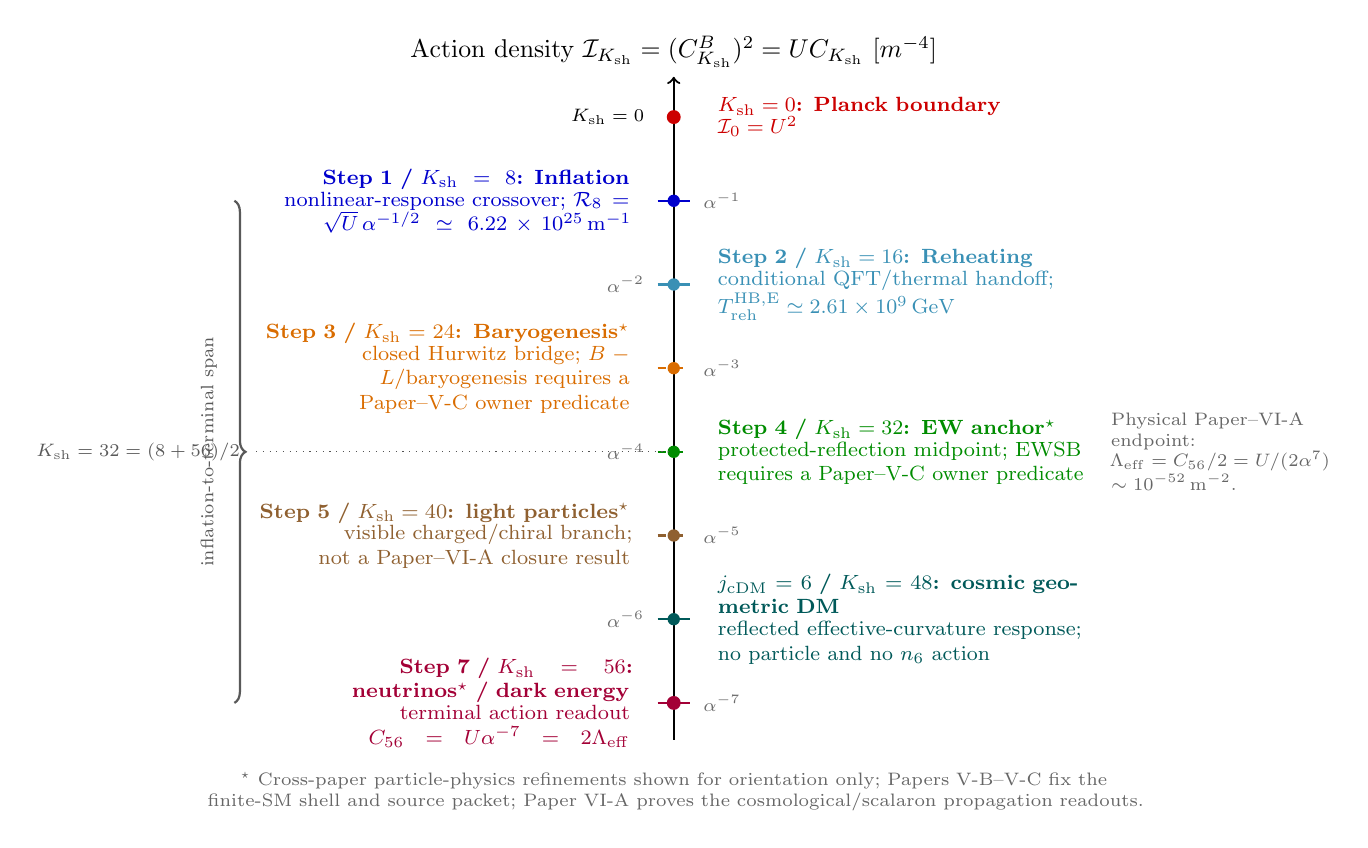
\begin{tikzpicture}[scale=0.93, transform shape,
    rung/.style={thick},
    coveredR/.style={font=\footnotesize, anchor=west, align=left, text width=5.05cm},
    coveredL/.style={font=\footnotesize, anchor=east, align=right, text width=5.05cm},
    importR/.style={font=\footnotesize, anchor=west, align=left, text width=5.05cm},
    importL/.style={font=\footnotesize, anchor=east, align=right, text width=5.05cm},
    ktagL/.style={font=\scriptsize, anchor=east},
    powtagL/.style={font=\scriptsize, anchor=east, gray!85!black},
    powtagR/.style={font=\scriptsize, anchor=west, gray!85!black}
]
    \draw[thick, ->] (0,1.0) -- (0,10.05);
    \node[anchor=south] at (0,10.05) {Action density $\mathcal I_{\Ksh}=(C^B_{\Ksh})^2=UC_{\Ksh}$ [$m^{-4}$]};

    \def\xText{0.48}
    \def\xTag{0.28}
    \def\yPlanck{9.50}
    \def\yStepOne{8.357}
    \def\yStepTwo{7.214}
    \def\yStepThree{6.071}
    \def\yStepFour{4.929}
    \def\yStepFive{3.786}
    \def\yStepSix{2.643}
    \def\yStepSeven{1.500}

    \fill[red!80!black] (0,\yPlanck) circle (2.7pt);
    \node[anchor=west, red!80!black, font=\footnotesize, align=left, text width=5.05cm] at (\xText,\yPlanck)
        {\textbf{$\Ksh=0$: Planck boundary}\\[-1pt]
        $\mathcal I_{0}=U^2$};
    \node[ktagL] at (-\xTag,\yPlanck) {$\Ksh=0$};

    \draw[rung, blue!80!black] (-0.22, \yStepOne) -- (0.22, \yStepOne);
    \fill[blue!80!black] (0,\yStepOne) circle (2.4pt);
    \node[coveredL, blue!80!black] at (-\xText,\yStepOne)
        {\textbf{Step 1 / $\Ksh=8$: Inflation}\\[-1pt]
        nonlinear-response crossover; $\mathcal R_8=\sqrt U\,\alpha^{-1/2}\simeq6.22\times10^{25}\,{\rm m}^{-1}$};
    \node[powtagR] at (\xTag,\yStepOne) {$\alpha^{-1}$};

    \draw[rung, cyan!70!black] (-0.22, \yStepTwo) -- (0.22, \yStepTwo);
    \fill[cyan!70!black] (0,\yStepTwo) circle (2.4pt);
    \node[coveredR, cyan!70!black] at (\xText,\yStepTwo)
        {\textbf{Step 2 / $\Ksh=16$: Reheating}\\[-1pt]
        conditional QFT/thermal handoff; $T_{\rm reh}^{\rm HB,E}\simeq2.61\times10^9\,{\rm GeV}$};
    \node[powtagL] at (-\xTag,\yStepTwo) {$\alpha^{-2}$};

    \draw[rung, orange!85!black, dashed] (-0.22, \yStepThree) -- (0.22, \yStepThree);
    \fill[orange!85!black] (0,\yStepThree) circle (2.4pt);
    \node[importL, orange!85!black] at (-\xText,\yStepThree)
        {\textbf{Step 3 / $\Ksh=24$: Baryogenesis$^{\star}$}\\[-1pt]
        closed Hurwitz bridge; $B\!-\!L$/baryogenesis requires a Paper--V-C owner predicate};
    \node[powtagR] at (\xTag,\yStepThree) {$\alpha^{-3}$};

    \draw[rung, green!55!black, dashed] (-0.22, \yStepFour) -- (0.22, \yStepFour);
    \fill[green!55!black] (0,\yStepFour) circle (2.4pt);
    \node[importR, green!55!black] at (\xText,\yStepFour)
        {\textbf{Step 4 / $\Ksh=32$: EW anchor$^{\star}$}\\[-1pt]
        protected-reflection midpoint; EWSB requires a Paper--V-C owner predicate};
    \node[powtagL] at (-\xTag,\yStepFour) {$\alpha^{-4}$};

    \draw[rung, brown!75!black, dashed] (-0.22, \yStepFive) -- (0.22, \yStepFive);
    \fill[brown!75!black] (0,\yStepFive) circle (2.4pt);
    \node[importL, brown!75!black] at (-\xText,\yStepFive)
        {\textbf{Step 5 / $\Ksh=40$: light particles$^{\star}$}\\[-1pt]
        visible charged/chiral branch; not a Paper--VI-A closure result};
    \node[powtagR] at (\xTag,\yStepFive) {$\alpha^{-5}$};

    \draw[rung, teal!70!black] (-0.22, \yStepSix) -- (0.22, \yStepSix);
    \fill[teal!70!black] (0,\yStepSix) circle (2.4pt);
    \node[coveredR, teal!70!black] at (\xText,\yStepSix)
        {\textbf{$j_{\rm cDM}=6$ / $\Ksh=48$: cosmic geometric DM}\\[-1pt]
        reflected effective-curvature response; no particle and no $n_6$ action};
    \node[powtagL] at (-\xTag,\yStepSix) {$\alpha^{-6}$};

    \draw[rung, purple!85!black] (-0.22, \yStepSeven) -- (0.22, \yStepSeven);
    \fill[purple!85!black] (0,\yStepSeven) circle (2.7pt);
    \node[coveredL, purple!85!black] at (-\xText,\yStepSeven)
        {\textbf{Step 7 / $\Ksh=56$: neutrinos$^{\star}$ / dark energy}\\[-1pt]
        terminal action readout $C_{56}=U\alpha^{-7}=2\CosmoEff$};
    \node[powtagR] at (\xTag,\yStepSeven) {$\alpha^{-7}$};

    \draw[decorate, decoration={brace, amplitude=4pt}, thick, gray!70!black]
        (-6.00,\yStepOne) -- (-6.00,\yStepSeven);
    \node[font=\scriptsize, align=center, rotate=90, gray!70!black] at (-6.35,{(\yStepOne+\yStepSeven)/2})
        {inflation-to-terminal span};
    \draw[gray!65!black, dotted] (-5.70,\yStepFour) -- (-0.05,\yStepFour);
    \node[font=\scriptsize, anchor=east, align=right, gray!70!black] at (-5.80,\yStepFour)
        {$\Ksh=32=(8+56)/2$};

    \node[anchor=west, align=left, font=\scriptsize, text width=3.0cm, gray!80!black]
        at (5.85,{(\yStepOne+\yStepSeven)/2})
        {Physical Paper--VI-A endpoint:\\
        $\CosmoEff=C_{56}/2=U/(2\alpha^7)$\\
        $\sim10^{-52}\,{\rm m}^{-2}$.};

    \node[anchor=north, align=center, font=\scriptsize, text width=12.8cm, gray!80!black]
        at (0,0.68)
        {$^{\star}$ Cross-paper particle-physics refinements shown for orientation only; Papers~V-B--V-C fix the finite-SM shell and source packet; Paper~VI-A proves the cosmological/scalaron propagation readouts.};
\end{tikzpicture}%
}
\caption{\textbf{Complete protected smooth-resolution hierarchy with typed role overlay.}  In native curvature-squared units ($m^{-4}$), adjacent octet rungs differ by one factor of $\alpha^{-1}$ in $\mathcal I_{\Ksh}=(C^B_{\Ksh})^2=UC_{\Ksh}$.  Paper~III derives all seven scalar landmarks, their unique common-rate hitting times, their ordering, and their neutral ratios.  The dimensionful curvature realization shown here is the closed-FLRW restriction proved in Theorem~\ref{p8:thm:flrw-determinant-owner-inheritance}; the particle-energy realization $E_{32},E_{40},E_{56}$ additionally uses the independent energy-ancestry port declared in Paper~V-B.  The displayed cosmological and finite-sector names are a separate role overlay governed by Theorem~\ref{p8:thm:typed-hierarchy-event-identification}: Paper~VI-A owns the proved gravitational predicates, while Papers~V-B--V-C own their particle and interaction predicates.  No shell-dependent source-phase multiplier is used in the scalar clock or its scale ratios.}
\label{p8:fig:hierarchy_corrected}
\end{figure}

\begin{proposition}[Global \(2I\) perturbation endpoint and local particle core]
\label{p8:prop:global-2I-local-particle-core}
The protected shell hierarchy displayed in Fig.~\ref{p8:fig:hierarchy_corrected}
has two distinct uses.  The inflationary low-momentum perturbation branch is a global
\(S^3\) branch and therefore may use the upper finite exceptional
endpoint
\[
    E_8:2I.
\]
The local visible-particle core used in Paper~V-B is instead the Hurwitz carrier
\[
    E_{32}:2T,
\]
together with its terminal interface and axial descendants \(E_{36}\) and
\(E_{40}\).  The upper and lower formal extrapolations \(E_0\) and \(E_{64}\)
are not admissible finite carriers: the former would lie above the global
binary-icosahedral closure, and the latter would lie below the exhausted neutral
reclosure branch.
\end{proposition}

\begin{proof}
Paper~I-A proves the mathematical exceptional data: \(2T\) is the Hurwitz
subgroup and \(2O=N_{S^3}(2T)\) is its ambient normalizer.  Paper~I-A assigns
no cosmological or particle role.  Theorem~\ref{p8:thm:2I-selection}
derives the present role assignment: \(2T\) is local, \(2O\) is the
normalizer/interface, and the global low-\(k\) mobile completion is \(2I\).
Its exact role is the sparse projector/comb, not a scalar-amplitude
normalization.  The
visible-particle mass readouts are local terminal readouts of the \(2T\) core
and its generated interface/axis supports.  No additional endpoint is generated
without inserting a larger exceptional finite subgroup above \(2I\) or an
independent residual carrier below the neutral reclosure.
\end{proof}


\begin{corollary}[Paper-I-A exceptional ranks with Paper-V-B readout chronology]
\label{p8:cor:paper-vi-platonic-readout-rank-handoff}
Paper~VI-A combines the Paper-I-A mathematical exceptional ranks with the Paper-V-B finite exceptional chronology over the same Hurwitz core; it does not use a nested subgroup-breaking chain.  With
\begin{equation}
\label{p8:eq:paper-vi-hurwitz-core-import}
    H=2T,
    \qquad |H|=24,
\end{equation}
the relevant Platonic readout ranks are
\begin{equation}
\label{p8:eq:paper-vi-readout-ranks-imported}
    \rho_H(2T)=1,
    \qquad
    \rho_H(2O)=2,
    \qquad
    \rho_H(2I)=5.
\end{equation}
The octahedral entry is the normalizer/interface readout
\begin{equation}
\label{p8:eq:paper-vi-normalizer-imported}
    N_{S^3}(2T)=2O,
\end{equation}
whereas the icosahedral entry is the global/terminal exceptional readout.  Hence
the common-unit rank gap determined by the Paper-I-A mathematics and used by the Paper-V-B chronology is
\begin{equation}
\label{p8:eq:paper-vi-readout-gap-imported}
    \Delta_{I/O}=|H|\bigl(\rho_H(2I)-\rho_H(2O)\bigr)=24(5-2)=72,
    \qquad
    \delta=\Delta_{I/O}^{-1/2}.
\end{equation}
This imported equality records a common-unit readout-rank difference.  It is not
the cardinality of a complement \(2I\setminus2O\), and it does not permit Paper~VI-A
to insert an additional finite support cell.
\end{corollary}
\begin{proof}
Paper~I-A proves the normalizer fork and the aggregation ranks \(1,2,5\).  Paper~V-B assigns those mathematical carriers to its local, interface, and terminal finite readouts before cosmological propagation begins.  Paper~VI-A therefore imports the Paper-V-B chronology while computing the common-unit gap \(24(5-2)=72\) from the Paper-I-A ranks.  Since the comparison is made in the common Hurwitz unit \(|H|\),
no nesting of \(2O\) inside \(2I\) is required or used.\qedhere
\end{proof}


\begin{theorem}[Imported protected structural resolution clock]
\label{p8:thm:protected-curvature-squared-shell-clock}
The neutral structural resolution clock is imported from the generated
owner trajectory of Theorem~\ref{p8:thm:flrw-determinant-owner-inheritance}:
\begin{equation}
\label{p8:eq:protected-action-shell-clock}
 \Ksh=8q_{\rm sp},
 \qquad
 \mathcal A_{\Ksh}=U\alpha^{-\Ksh/8},
 \qquad
 \mathcal R_{\Ksh}=\sqrt{\mathcal A_{\Ksh}}
 =\sqrt U\,\alpha^{-\Ksh/16}.
\end{equation}
At the integer crossings,
\begin{equation}
\label{p8:eq:protected-cosmological-K-ladder}
 \Ksh=8,16,24,32,40,48,56.
\end{equation}
Adjacent main landmarks satisfy
\begin{equation}
\label{p8:eq:action-shell-one-step}
 \mathcal A_{\Ksh+8}=\alpha^{-1}\mathcal A_{\Ksh},
 \qquad
 \mathcal R_{\Ksh+8}=\alpha^{-1/2}\mathcal R_{\Ksh}.
\end{equation}
The terminal root and action scales are
\begin{equation}
\label{p8:eq:terminal-action-shell-readout}
 \mathcal R_{56}=\sqrt U\,\alpha^{-7/2},
 \qquad
 C_{56}=\mathcal A_{56}=\mathcal R_{56}^{\,2}
 =U\alpha^{-7}=2\CosmoEff.
\end{equation}
Thus the hierarchy is natively \(U\)-owned, with the primitive geometric actualization \(\mathcal K_p=6/\Rmom^2,\ U=(3/\pi)\mathcal K_p\).
Paper~VI-A, together with the finite-sector prefix, may attach a physical
readout name only through the typed predicate of
Theorem~\ref{p8:thm:typed-hierarchy-event-identification}; it does not alter
the derived scales or the smooth Paper--III action.  The symbol \(q_{\rm sp}\)
here is structural; no equality with cosmic time or with a generic physical
scalaron trajectory is implied.
\end{theorem}

\begin{proof}
The equations are the Paper--III generated positive-character export after
the closed-FLRW owner inheritance proved above.  Positive functional calculus
gives \(\mathcal R_{\Ksh}=\sqrt{\mathcal A_{\Ksh}}\).  The Paper--V-B and
Paper--V-C carrier ledgers provide downstream finite-sector predicates and
projectors.  Their composition changes the readout at a landmark but
introduces no new hierarchy factor, crossover scale, or action coefficient.
No additional Planck/Newton owner ratio is required.
\end{proof}

\begin{remark}[Structural clock without a shell-source phase selector]
The exact seven-rung scalar hierarchy, its reflected midpoint and its
finite-sector role predicates have no Reeb standing-wave phase assignment.
In particular, the primitive Hopf/Reeb phase geometry does not supply a
shell-by-shell physical source-phase multiplier or a CP-asymmetry datum.
All slow-roll, scalar-amplitude, and conditional reheating readouts remain
unchanged; their assumptions and owner predicates are those stated above.
\end{remark}


\begin{corollary}[Protected non-carrier rungs in the cosmological clock]
\label{p8:cor:protected-noncarrier-rungs-K24-K48}
The rungs \(\Ksh=24\) and \(\Ksh=48\) are geometrically distinguished but are not independent homogeneous vacuum endpoints or new particle endpoints.  The rung
\begin{equation}
\Ksh=24=3\cdot 8
\end{equation}
is the closed Hurwitz/24-cell bridge count, while
\begin{equation}
\Ksh=48=6\cdot8=56-8
\end{equation}
is the one-octet-before-terminal scalaron-orientation rung.  Thus \(\Ksh=24\) may support a conditional \(B-L\) bridge only when the
corresponding Paper~V-C owner predicate is independently satisfied.
The \(\Ksh=48\) label denotes a structural separator, not an independent
homogeneous vacuum source; the minimal homogeneous cosmological branch
supplies no additional constant-term readout at either rung.
\end{corollary}

\begin{proof}
The closed finite carrier count imported from Paper~I-A is the Hurwitz/24-cell count \(L_\star=24\).  On the seven-step action-density clock this is a closed count rather than a new endpoint; it is therefore available as a bridge/complement count.  A physical \(B-L\) handoff requires its independent source/action predicate, and the count is not a second vacuum constant.  Similarly, \(\Ksh=48=56-8\) is singled out by removal of one protected octet from the terminal index.  It is consequently the natural orientation/separator rung immediately before the terminal static readout.  Since the minimal \(\Dcl\) branch permits only the homogeneous terminal constant-term readout \eqref{p8:eq:terminal-action-shell-readout}, adding independent vacuum constants at \(\Ksh=24\) or \(\Ksh=48\) would be an inserted profile outside the uninserted branch.\qedhere
\end{proof}


\begingroup
\scriptsize
\setlength{\tabcolsep}{4pt}
\renewcommand{\arraystretch}{1.08}

\begin{xltabular}{\linewidth}{@{}
  >{\raggedright\arraybackslash}p{3.8cm}
  >{\raggedright\arraybackslash}X
  >{\raggedright\arraybackslash}p{3.3cm}
@{}}
\caption[Geometric cosmology outputs]{Geometric cosmology outputs.}
\label{p8:tab:geometric-outputs}\\

\toprule
\textbf{Quantity}
& \textbf{Exact expression}
& \textbf{Value / readout} \\
\midrule
\endfirsthead

\toprule
\textbf{Quantity}
& \textbf{Exact expression}
& \textbf{Value / readout} \\
\midrule
\endhead

\midrule
\multicolumn{3}{r}{\emph{Continued on next page}}\\
\bottomrule
\endfoot

\bottomrule
\endlastfoot


\gpsection{Geometric normalisations}

Einstein--Hilbert prefactor
& \(\Omega_3/(2\sqrt{\pi})^4\)
& \(1/8\) \\

Stabilisation correction \(\delta\)
& \(|\Phi(E_6)|^{-1/2}=1/(6\sqrt2)\)
& \(0.11785113\) \\

Optional uniform-rank arithmetic \(H_8\)
& \(\sum_{k=1}^8 k^{-1}=761/280\), only for \(\mu_k=1/8\)
& \(2.71785714\) (non-native) \\

Planck-scale curvature \(U\)
& \(c^3/(2\pi\hbar G)\)
& \(6.09\times10^{68}\,{\rm m}^{-2}\) \\

Hierarchical step \(\alpha\)
& \(\exp\!\bigl((2\pi)^2+\delta\bigr)\)
&
\mathcell{
1.571958279122504\\
{}\times10^{17}
} \\


\gpsection{Protected shell hierarchy}

Protected action-density clock
&
\mathcell{
\Ksh\in8\ZZ,\\
\mathcal I_{\Ksh+8}=\alpha^{-1}\mathcal I_{\Ksh},\\
\mathcal R_{\Ksh}=\sqrt U\,\alpha^{-\Ksh/16}
}
&
\mathcell{
\Ksh\in\{8,16,24,32,\\
40,48,56\}
} \\

Inflationary root-wavenumber shell
&
\mathcell{
{\Ksh}_{\rm inf}=8,\\
\mathcal R_8=\sqrt U\,\alpha^{-1/2}
}
& \(\simeq6.22\times10^{25}\,{\rm m}^{-1}\) \\

Reheating root-wavenumber shell
&
\mathcell{
{\Ksh}_{\rm reh}=16,\\
\mathcal R_{16}=\sqrt U\,\alpha^{-1}
}
&
\mathcell{
\simeq1.57\times10^{17}\\
{\rm m}^{-1}
} \\


\gpsection{Active Laurent inflation and optional MRESP comparison}

Full-index Laurent coefficient
&
\(Q=8\sqrt\alpha\)
&
\(8\sqrt\alpha\) on the generated section \\[2pt]

Optional MRESP Hessian-equivalent scale \(M_{\rm H}\)
&
\mathcell{
M_{\rm H}^2=\dfrac{\hbar^2U}{48\alpha^{1/2}c^2}=\dfrac{\hbar^2U}{48\alpha^{1/2}c^2}
}
&
\mathcell{3.53\times10^{13}\\ {\rm GeV};\ \text{not a pole mass}} \\

Pivot e-fold count \(N_*\)
& Explicit calibration for either inflation branch
& \(56\) \\

Active Laurent scalar index \(n_s\) on the generated branch
& Eq.~\eqref{p8:eq:laur27-starobinsky-observables}; exact Laurent correction below displayed precision
& \(0.965587116277\) \\

Active Laurent tensor ratio \(r\) on the generated branch
& Eq.~\eqref{p8:eq:laur27-starobinsky-observables}
& \(0.00338038887247\) \\

Active Laurent scalar amplitude \(A_s^{(S^3)}\) on the generated branch
& Eq.~\eqref{p8:eq:laur27-starobinsky-observables}
& \(3.072107140762\times10^{-9}\) \\

Optional MRESP visibility \(u_*\) on the generated branch
& \(u(R_*)=\log(R_*/C_{56})/\log(U/C_{56})\)
& \(0.9343324910\) \\

Optional MRESP scalar index \(n_s\) on the generated branch
& \(1-6\epsilon_*+2\eta_*\)
& \(0.9629607784\) \\

Optional MRESP tensor ratio \(r\) on the generated branch
& \(16\epsilon_*\)
& \(0.00288427536\) \\

Optional MRESP tensor tilt \(n_t\) on the generated branch
& \(-2\epsilon_*\)
& \(-3.60534420\times10^{-4}\) \\

Optional MRESP running \(\alpharun\) on the generated branch
& \(16\epsilon_*\eta_*-24\epsilon_*^2-2\xi_*^2\)
& \(-5.97692\times10^{-4}\) \\

Optional MRESP scalar amplitude \(A_s^{(S^3)}\) on the generated branch
& \(V_*/(24\pi^2\Mplbar^4\epsilon_*)\) on the smooth comparison action
& \(3.86944262\times10^{-9}\) \\


\gpsection{Late-time cosmology}

Dark-energy scale \(\CosmoEff\)
&
\mathcell{
C_{56}:=\mathcal R_{56}^{\,2}=U\alpha^{-7},\\
C_{56}=2\CosmoEff
}
&
\mathcell{
1.2835\times10^{-52}1\\
{\rm m}^{-2}
} \\

Spatial curvature \(\Omega_k\)
&
\mathcell{
N_{P\to{\rm acc}}=\dfrac13\log\!\left(\dfrac{\rho_{m,P}}{2\rho_\Lambda}\right),\\
\text{depends on the dust integration constant}
}
& no carrier-only numerical prediction \\


\gpsection{Hopf and galactic-scale outputs}

Hopf ruler coefficient \(\kappa_{\rm Hopf}\)
& \(761/(13440\sqrt2)\)
& \(0.0400378\) \\

RAR terminal local acceleration \(a_{56}\)
& \(c^2\sqrt{C_{56}}/(4\pi)\)
&
\mathcell{1.146\times10^{-10}1\\ {\rm m\,s^{-2}}} \\

Log-periodic period \(\Delta\ln k\)
& \(((2\pi)^2+\delta)/7\)
& \(5.65660982\) \\

Intrinsic Hopf amplitude \(A_{\rm Hopf}\)
& \(2\delta/\pi=1/(3\sqrt2\pi)\)
& \(7.50\%\) \\

\end{xltabular}

\endgroup

\clearpage
\begingroup
\scriptsize
\setlength{\tabcolsep}{4pt}
\renewcommand{\arraystretch}{1.08}

\begin{xltabular}{\linewidth}{@{}
  >{\raggedright\arraybackslash}p{2.8cm}
  >{\raggedright\arraybackslash}X
  >{\raggedright\arraybackslash}p{5.8cm}
@{}}
\caption[Determinant outputs and validation pushforwards]{Determinant outputs and validation pushforwards.}
\label{p8:tab:determinant-validation-outputs}\\

\toprule
\textbf{Quantity}
& \textbf{Exact expression}
& \textbf{Value / readout} \\
\midrule
\endfirsthead

\toprule
\textbf{Quantity}
& \textbf{Exact expression}
& \textbf{Value / readout} \\
\midrule
\endhead

\midrule
\multicolumn{3}{r}{\emph{Continued on next page}}\\
\bottomrule
\endfoot

\bottomrule
\endlastfoot


\gpsection{Amplitude and reionization interface}

Native \(2I\) pivot transfer
&
\mathcell{
\widehat T_{2I}(k_*)=1,\\
\text{no smooth }2I\text{ envelope multiplier is generated}
}
& no additional native pivot normalization \\

CMB amplitude combination
& \(A_s^{\rm CMB}=A_s^{(S^3)}\,\mathcal N_{\rm pert}(k_*)e^{-2\tau_{\rm reio}}\)
& \(\mathcal N_{\rm pert}\) is a typed perturbation/readout interface \\


\gpsection{Dark-sector and halo interfaces}

Dark-sector/RAR terminal scale
&
\mathcell{
C_{56}:=U\alpha^{-7},\\
a_{56}=\dfrac{c^2}{4\pi}\sqrt{C_{56}}
}
&
\mathcell{a_{56}=1.146\times10^{-10}1\\ {\rm m\,s^{-2}}} \\

Cosmic-DM response coordinate
&
\mathcell{
j_{\rm cDM}=6\ \text{(final-octet separator)},\quad K_{\rm cDM}=48,\\
C_6=U\alpha^{-6}=\alpha C_7
}
&
\mathcell{
\text{effective curvature-fluid label;}\\
\text{not }n_6,\text{ not a mass, and not a particle}
} \\


\gpsection{Paper--VI-B downstream cosmological readouts}

Rulers, \(H_0\), growth, horizon, and BBN
& \(\text{fixed Paper--VI-A gravitational packet}\longrightarrow\text{Paper--VI-B propagation}\)
& delegated downstream readouts \\
\noalign{\penalty -10000}
\gpsection{Branch-separated conditional reheating readouts}

Reheating temperature \(k_B T_{\rm reh}\)
&
\mathcell{
T_{16}^{E}(\xi)
=\left(\dfrac{30\xi}{\pi^2g_*}\right)^{1/4}
\mathcal I_{16}^{1/4},\\
T_{\rm reh}^{(0,E)}
=
\left(\dfrac{90}{\pi^2g_*}\right)^{1/4}
\sqrt{\Gamma_s\bar M_{\rm Pl}}\\
=
C_{\rm reh}\sqrt{U}\alpha^{-3/8},\\
g_*=427/4
}
&
\mathcell{
5.0457\times10^9\xi^{1/4}\,{\rm GeV}\ \text{under }(\mathrm{REH}_{16}[\xi]);\\
2.9588\times10^9\,{\rm GeV}\ \text{under }(\mathrm{MASS}_{\rm UV});\\
2.605\times10^9\,{\rm GeV}\ \text{(decay visible)},\\
2.6019\times10^9\,{\rm GeV}\ \text{(direct }\xi=\delta_{\rm geom}\text{ visible)},\\
\text{both also require }(\mathrm{DEM}_{15})+(\mathrm H_{\rm kin})
} \\

\end{xltabular}

\endgroup


\paragraph{Row-status note for Table~\ref{p8:tab:fine_tuning}.}
In this comparison table, entries in the Hopf--Born column marked ``Derived'' are \RowTheorem{} or \RowBridge{} only for the finite geometric hierarchy stated in the row.  Rows involving reheating temperature, inner rotation-curve fits, core sizes, propagated observables, Hubble-tension comparisons, or parameter counts are \RowComparison{} or \RowOpen{} at the observational-interface level and do not select the Hopf carrier or shell clock.  The final row counts adjustable geometric constants inside the reduced kernel, not nuisance parameters, survey windows, propagation choices, catalog selections, covariance matrices, or likelihood parameters used in external validation.


\begin{table}[H]
\centering
\small
\renewcommand{\arraystretch}{1.5}
\setlength{\tabcolsep}{4pt}


\par\noindent
\begingroup
\centering
\small
\setlength{\tabcolsep}{3pt}
\renewcommand{\arraystretch}{1.18}

\begin{tabularx}{\textwidth}{|
>{\RaggedRight\arraybackslash}p{0.22\textwidth}|
Y|Y|Y|}
\hline
\textbf{Parameter / Feature}
&
\makecell[l]{\textbf{\LCDM}\\\textbf{(Standard)}}
&
\makecell[l]{\textbf{Phenom.}\\\textbf{Starobinsky}\\\textbf{($\scal+\scal^2$)}}
&
\makecell[l]{\textbf{Hopf-Born}\\\textbf{(GP-closed)}} \\
\hline
\hline

\textbf{Inflationary Potential}
& Input (assumed $V(\phi)$)
& Input ($\scal^2$ term assumed)
& \textbf{Derived conditional smooth branch} (not a global quadratic ansatz) \\
\hline

\textbf{Inflaton Mass ($M$)}
& Tuned to $A_s$ ($\sim 10^{13}$ GeV)
& Tuned to $A_s$ (free parameter)
& \textbf{Hessian-equivalent scale only}
  ($M_{\rm H}\propto\alpha^{-1/4}$; pole-mass identification open) \\
\hline

\textbf{Duration ($N$ e-folds)}
& Tuned (requires $N \sim 50\text{--}60$)
& Tuned (depends on reheating)
& \textbf{Explicit dimensionless pivot calibration}
  ($N_*=D_\star=56$; dynamical duration open) \\
\hline

\textbf{Reheating ($T_{\text{reh}}$)}
& Unknown / free
& Model-dependent
& \textbf{Derived $K=16$ scale; conditional physical readout}
  ($\sim 3 \times 10^9$ GeV on either displayed source branch) \\
\hline

\textbf{Dark Energy ($\Cosmo$)}
& Tuned ($\sim 10^{-120}$)
& Added by hand ($\Cosmo$)
& \textbf{Derived} ($\alpha^{-7}$ hierarchy) \\
\hline

\textbf{Dark Matter}
& Input (WIMP/Axion)
& Input (added by hand)
& \textbf{Derived response} (scalaron/\allowbreak RAR shell) \\
\hline

\textbf{Galaxy Halos (Cores)}
& strong tension without baryonic feedback modeling
& N/A
& deep law derived (inner fits interface) \\
\hline

\textbf{Hubble/ruler readout}
& Downstream likelihood problem
& Downstream likelihood problem
& \textbf{Paper--VI-B propagation} \\
\hline
\hline

\textbf{Adjustable geometric constants in the reduced kernel}
& \textbf{6} (baseline + feedback at model level)
& \textbf{1 + \LCDM\allowbreak{} params}
& \textbf{0} (validation pushforwards remain external maps) \\
\hline

\end{tabularx}

\par
\endgroup

\caption[Fine-tuning comparison]{Fine-tuning comparison with reduced-kernel status labels.}
\label{p8:tab:fine_tuning}

\end{table}

\TableNotes{Comparison of the standard cosmological model (\LCDM), the phenomenological Starobinsky inflation model, and the derived Hopf--Born framework. Standard approaches introduce independent mass scales ($M$), vacuum-energy parameters ($\Cosmo$), or baryonic-feedback prescriptions; the Hopf--Born framework assigns the corresponding hierarchy and terminal scalaron/RAR response to fixed spectral/contact kernels of the $S^3$ Hopf carrier, subject to the validation boundaries stated below. Inner rotation-curve fits, core sizes, and propagated observables remain interface-level outputs.}


% Source Paper VI-A, original line 19078
\subsection{Separated-scale regular Born--Legendre gravity and the lapse potential}
\label{p8:app:bare-born-legendre}
This appendix uses the regular bare reconstruction of Paper~III-F,
Theorem~\ref{p3f:thm:bare-born-potential-criterion}.  It does not replace
the active dressed Laurent branch or select a junction profile.  Its purpose
is to keep the UV curvature susceptibility and IR terminal jet separate and
to compute the exact same-action potential on the regular terminal member.

\begin{proposition}[Lapse extraction of the same-action potential]
\label{p8:prop:bare-legendre-lapse-potential}
For a supplied nondegenerate local metric action written as
\(\overline{\mathcal F}(R)\leftrightarrow XR-V(X)\), take
\(ds^2=-N^2dt^2+a^2d\Sigma_k^2\), with proper-time orientation fixed.
After integration by parts with the corresponding boundary term handled,
and suppressing the common action factor and homogeneous spatial volume,
the reduced Lagrangian is
\[
 L=-\frac{6aX\dot a^2}{N}
   -\frac{6a^2\dot a\dot X}{N}+6kNaX-Na^3V(X).
\]
In vacuum, lapse variation followed by \(N=1\) gives
\begin{equation}
 \label{p8:eq:bare-legendre-lapse-potential}
 \boxed{3X(H^2+k/a^2)=\frac{V}{2}-3H\dot X,\qquad
 V(X(R))=R\overline{\mathcal F}'-\overline{\mathcal F}.}
\end{equation}
Thus the potential enters the Lagrangian with a minus sign and the lapse
constraint with the displayed positive sign. It is the potential component,
not the entire gravitational Hamiltonian or a relative scalar first
variation.
\end{proposition}
\begin{proof}
Use
\[
 R=6\left(\frac{\ddot a}{aN^2}
 +\frac{\dot a^2}{a^2N^2}
 -\frac{\dot a\dot N}{aN^3}+\frac{k}{a^2}\right).
\]
The term containing \(\ddot a\) is integrated once; its \(\dot N\)
contribution cancels the displayed \(\dot N\) term. This gives \(L\).
Its lapse derivative is
\[
 \frac{\partial L}{\partial N}
 =\frac{6aX\dot a^2}{N^2}
  +\frac{6a^2\dot a\dot X}{N^2}+6kaX-a^3V.
\]
Set it to zero, choose proper time, and divide by \(2a^3\).
The potential identity is the auxiliary-field equation from Paper~III-F.
This is the same zero-derivative term already present in
Corollary~\ref{p8:cor:closed-flrw-friedmann-derived}, with all zero-order
terms included in \(\overline{\mathcal F}\).
\end{proof}

\begin{proposition}[Complete homogeneous canonical constraint]
\label{p8:prop:complete-flrw-canonical-constraint}
For the preceding reduced Lagrangian, with \(a>0\) and \(N\ne0\),
the canonical momenta and constraint are
\[
 \Pi_a=-\frac{12aX\dot a+6a^2\dot X}{N},\qquad
 \Pi_X=-\frac{6a^2\dot a}{N},\qquad \Pi_N=0,
\]
\[
 H_{\rm can}=N\mathcal C,\qquad
 \boxed{\mathcal C=\frac{X\Pi_X^2}{6a^3}
 -\frac{\Pi_a\Pi_X}{6a^2}-6kaX+a^3V(X).}
\]
The total Hamiltonian adds the multiplier of the primary constraint
\(\Pi_N=0\); its preservation yields \(\mathcal C=0\).
The symbols \(\Pi_a,\Pi_X\) are canonical momenta, distinct from the
fluid-pressure notation \(p_X\) elsewhere in this paper.
\end{proposition}
\begin{proof}
Differentiate \(L\) in \(\dot a,\dot X\). The velocity Hessian has
determinant \(-36a^4/N^2\), so these two velocities are invertible:
\[
 \dot a=-N\Pi_X/(6a^2),\qquad
 \dot X=N(2X\Pi_X/a-\Pi_a)/(6a^2).
\]
Substitution in \(\Pi_a\dot a+\Pi_X\dot X-L\) gives \(H_{\rm can}\).
The Ricci reduction used the total derivative
\(d(6a^2X\dot a/N)/dt\); its boundary convention is held fixed.
Lapse variation agrees with
\eqref{p8:eq:bare-legendre-lapse-potential}.
\end{proof}
For the regular separated branch put
\[
 \overline f_{\rm reg}(R)
 =(R-C)+\frac{(R-C)^2}{U+C},
 \qquad
 \overline{\mathcal F}_{\rm reg}=U\overline f_{\rm reg}.
\]
Its conjugate coefficient and dimensionful same-action potential are
\[
 X=\overline{\mathcal F}_{\rm reg}'
 =U\left[1+\frac{2(R-C)}{U+C}\right],
 \qquad
 \boxed{V(X)=R X-\overline{\mathcal F}_{\rm reg}
 =\frac{U}{U+C}(R^2+UC).}
\]
Writing \(\chi=X/U\), this is equivalently
\begin{equation}
\label{p8:eq:regular-separated-jordan-potential}
 \boxed{
 V_J(\chi):=\frac{V(X)}U
 =C\chi+\frac{U+C}{4}(\chi-1)^2,\qquad
 R=C+\frac{U+C}{2}(\chi-1).}
\end{equation}
Thus \(\chi=1\) is exactly the terminal point \(R=C\), and
\(V_J(1)=V_J'(1)=C\).

\begin{corollary}[Regular separated Born--Legendre consequences]
\label{p8:cor:conditional-bare-born-legendre}
On the regular terminal member,
\[
 \boxed{
 R\overline f_{\rm reg,R}-\overline f_{\rm reg}
 =\frac{R^2+UC}{U+C}=R g_{\rm eff}(R).}
\]
Moreover
\[
 \overline f_{\rm reg,R}
 =1+\frac{2(R-C)}{U+C},
 \qquad
 \overline f_{\rm reg,RR}=\frac{2}{U+C}>0.
\]
The constant-curvature vacuum equation has the root
\[
 \boxed{
 R_{\rm dS}=\frac{2UC}{U-C},
 \qquad
 \chi_{\rm dS}=\frac{U+C}{U-C},
 \qquad
 m_s^2=\frac{U-C}{6}}
\]
in curvature units \(c=1\).  This vacuum lies in the supplied reciprocal
interval \([C,U]\) when \(U\ge3C\).  These statements concern the regular
bare branch and do not replace the active dressed Laurent history.
\end{corollary}
\begin{proof}
The potential identity is Paper~III-F,
Theorem~\ref{p3f:thm:bare-born-potential-criterion}.  For the vacuum,
\[
 R\overline f_R-2\overline f
 =\frac{CR+2CU-RU}{U+C},
\]
which vanishes at \(2UC/(U-C)\).  Finally
\[
 \frac{\overline f_R-R\overline f_{RR}}
      {3\overline f_{RR}}
 =\frac{U-C}{6}.
\]
The interval condition is
\(2UC/(U-C)\le U\iff U\ge3C\).
\end{proof}

\begin{corollary}[Historical copied-response endpoint as an affine displacement]
\label{p8:cor:sharp-regular-terminal-affine-displacement}
For comparison with pre-v2.63 releases, the lower undressed copied-response
TERM--REN representative was
\[
 f_{\rm sharp}(R)
 =R+\frac{R^2+UC}{U+C}-2C.
\]
It obeys the exact relation
\begin{equation}
\label{p8:eq:sharp-regular-affine-difference}
 \boxed{
 f_{\rm sharp}(R)-\overline f_{\rm reg}(R)
 =\frac{2C}{U+C}(R-C).}
\end{equation}
Hence
\[
 f_{\rm sharp}''=\overline f_{\rm reg}'',
 \qquad
 f_{\rm sharp}'(C^+)-\overline f_{\rm reg}'(C)
 =\frac{2C}{U+C},
\]
while their Legendre potentials differ by the constant
\[
 R f_{\rm sharp}'-f_{\rm sharp}
 =R g_{\rm eff}(R)+\frac{2C^2}{U+C}.
\]
Therefore the historical terminal slope atom and the historical
Born--Legendre mismatch were the same affine junction datum.  The retained
v2.63 action is instead the inverse-Euler Legendre primitive and already
selects the regular \(C^1\) member.  This corollary is diagnostic provenance only; the derived exact junction
selects neither a second action member nor an independent microscopic profile.
\end{corollary}
\begin{proof}
Expand both quadratics and subtract.  Applying
\(R\partial_R-1\) to the affine difference gives
\(2C^2/(U+C)\).
\end{proof}

\paragraph{Canonical-constraint consequence.}
In Proposition~\ref{p8:prop:complete-flrw-canonical-constraint} the potential
term is therefore, on the regular separated branch,
\[
 \boxed{
 V(X)=CX+\frac{U+C}{4U}(X-U)^2.}
\]
The lapse/Hamiltonian constraint retains both scales explicitly.  The
curvature Hessian fixes the quadratic coefficient, while the terminal jet
fixes the affine completion.  No action-level anti-contact Born law is
required.

\begin{remark}[Terminal quotient and active sharp branch remain distinct]
\label{p8:rem:bare-legendre-terminal-not-active-freeze}
For the regular member \(\chi=1\) implies \(R=C\) directly from
\eqref{p8:eq:regular-separated-jordan-potential}; this is precisely why the
regular terminal jet closes the bare Born--Legendre relation.  The active
positive-part Laurent realization remains the sharp branch with its endpoint
measure until a physical junction theorem selects \(C^1\) matching.  Thus
this appendix removes the former scale-mixed Born--Legendre obstruction but
does not silently change the realized inflationary branch, its dressing, or
its cosmological history.
\end{remark}

\begingroup
\small
\RaggedRight
\hyphenpenalty=300
\exhyphenpenalty=300
\emergencystretch=6em
% BEGIN FRAMEWORK v2.223: capped candidate branch and cosmological scope
% Source Paper VI-A, original line 19303
\subsection{The capped working action and its cosmological comparison domain}
\label{p8:sec:v223-cap-candidate}
Theorem~\ref{p3e:thm:v223-exact-cap-reduction} gives the exact candidate
\[
 f_c(R)=PR+R^2B(R)-\sigma^2/B(R)^2,\qquad
 B(R)=B_U+\frac{2(B_I-B_U)}{1+\sqrt{1+(R/R_s)^2}},
\]
from specified boundary and sourced ports.  Its smooth non-null boundary
uses the total $f_c'$ including the source derivative; its metric and
trace equations are Corollary~\ref{p3f:cor:v223-cap-metric}.  The phase
curvature comparison and finite Clifford endpoint are stated in
Proposition~\ref{p3d:prop:v223-curvature-clock}.  The endpoint $C_7$ is
positive and its small dressing error is quantified; it is not silently
replaced by $R=0$ or an off-domain freeze.

\begin{remark}[Current working action retains its native-identification obligations]
\label{p8:rem:v223-cap-status}
The cap is the \emph{working action for subsequent gravitational
calculations}, not an unconditionally proven identification with the
native microscopic action. Its remaining native operator, source and
density maps are listed in Remark~\ref{p3e:rem:v223-native-selection}.
The prior $n_4\mid n_7$ cosmological response remains a result only
under its own assumptions and is not a second term in the cap action.
Proposition~\ref{p3e:prop:v288-cap-laurent-nonidentification} proves that
the two one-variable densities are unequal in a shared curvature chart.
Cosmological histories, perturbations, particle production,
dark-sector responses and observational comparisons must therefore be
recomputed from the cap's complete action and actual boundary/state
data; their earlier numerical values do not transfer by relabelling.
\end{remark}

% BEGIN FRAMEWORK v2.288: CAPPED VACUUM COSMOLOGICAL TARGET
\begin{corollary}[Capped working-action vacuum location and positive scalaron sign]
\label{p8:cor:v288-cap-vacuum-target}
On the source-free constant-curvature domain of the current capped
\emph{working action}, with the complete action and boundary conditions
of Theorem~\ref{p3e:thm:v223-exact-cap-reduction}, retain the hierarchy
anchors of Proposition~\ref{p3d:prop:v223-curvature-clock}. Define
\(C_7^{(P)}:=P\alpha^{-7}=R_s^2/P\).
Then Theorem~\ref{p3f:thm:v288-cap-vacuum-root-stability} gives exactly
one positive vacuum root and the sharp owner-typed bracket
\[
 \boxed{C_7^{(P)}<R_*<2C_7^{(P)},\qquad m_s^2(R_*)>0.}
\]
The relative distance below $2C_7^{(P)}$ is bounded by
$4(1-B_U/B_I) B_I/(P/R_s)^4$. Only on an independently established
$P=U$ curvature-owner comparison does this become
$C_7<R_*<2C_7$ for the separate $U$-owned $C_7$.
In particular the vacuum field equation admits the explicit
closed-$S^3$ de~Sitter solution family
\[
 \boxed{N(t)=1,\qquad
 a(t)=\sqrt{\frac{12}{R_*}}
 \cosh\!\left(\sqrt{\frac{R_*}{12}}(t-t_0)\right),
 \quad t_0\in\mathbb R.}
\]
This is an available classical solution of the \emph{conditional}
metric action, not a selected occurring history or a result transferred
from the historical Laurent dressing.
\end{corollary}
\begin{proof}
The source-free constant-curvature trace of
Corollary~\ref{p3f:cor:v223-cap-metric} is
$R f_c'-2f_c=0$. The hypotheses and the bounds are verified by
Theorem~\ref{p3f:thm:v288-cap-vacuum-root-stability}.
The owner comparison follows from the phase curvature chart of
Proposition~\ref{p3d:prop:v223-curvature-clock}.
The sign of the scalaron parameter uses the same theorem's strict
positivity of $f_c''$ and $f_c'-Rf_c''$ at its unique root.
Set $H_*^2=R_*/12$. For $a=H_*^{-1}\cosh(H_*(t-t_0))$ one has
$\ddot a/a=H_*^2$ and $(\dot a^2+1)/a^2=H_*^2$.
The closed-$S^3$ FLRW curvature chart of
Theorem~\ref{p3e:thm:v287-s3-acceleration-hessian} gives
$R=12H_*^2=R_*$, and direct FLRW Ricci evaluation gives
$R_{\mu\nu}=3H_*^2g_{\mu\nu}=R_*g_{\mu\nu}/4$.
On constant $R$, all derivatives of $f_c'(R)$ vanish. Therefore the
metric equation of Corollary~\ref{p3f:cor:v223-cap-metric} reduces to
$f_c'(R_*) R_*g_{\mu\nu}/4-f_c(R_*)g_{\mu\nu}/2=0$,
which is exactly its already proved vacuum trace equation.
\end{proof}
% END FRAMEWORK v2.288: CAPPED VACUUM COSMOLOGICAL TARGET

Finite-collar scalar action and canonical boundary errors are bounded in
Theorem~\ref{p3f:thm:v223-collar-error}.  They do not bound cosmological
solution errors without the appropriate evolution and initial-data
estimates.  The positive-fibre extension is an analytic operator
construction; it neither changes the native eight-dimensional geometry
nor identifies its response fibres with physical spacetime.  No new
inflation, QCD, particle spectrum or dark-sector prediction follows
from the candidate constructor alone.
% END FRAMEWORK v2.223: capped candidate branch and cosmological scope


% BEGIN FRAMEWORK v2.228: CHARGED ORIGIN AND CHARACTER TESTS
% Source Paper VI-A, original line 19343
\subsection{Charged source certificates in cosmological applications}
\label{p6a:sec:v228-charged-source-scope}
Where a cosmological calculation consumes the noncentral charged mass
source, it inherits Definition~\ref{p5:def:v228-hierarchy-origin} and
Proposition~\ref{p5:prop:v228-charged-origin-scope}.
This condition is attached to that source arrow; it does not alter the
independently derived gravitational owner, the rooted primitive source,
or pure geometric carrier counts. A finite mass-only identity proved by
Corollary~\ref{p5b:cor:v228-source-character-test} or
\ref{p5b:cor:v228-source-fibre-readout} must still be transported through
the actual plasma/state, interaction, history and comparison maps consumed
by the claimed observable.

% END FRAMEWORK v2.228: CHARGED ORIGIN AND CHARACTER TESTS

% \printbibliography relocated to the end of the active volume
\endgroup



\section{Scalaron, metric variation, trace response and conserved source work}
\label{p6a:sec:organized-a3}
The single retained scalaron, complete metric variation, Ward constraints and coupled source work must be evaluated within one realized action and state. Auxiliary finite-jet and curvature estimates appear in Paper~VI-C.

% The technical proof companion retains auxiliary original labels.
% Source Paper VI-A, original line 3985
\subsection{Scalar-Tensor Form and Regime Analysis}

The Einstein-frame map used in this section is the SI-consistent one defined in
Sec.~\ref{p8:sec:std_cosmo_reductions}; we therefore work only with the
dimensionless conformal factor \(F(\scal)\) and the derived observables.


% Source Paper VI-A, original line 7152
\subsubsection{Exact nonlinear scalaron law, constrained flow, and energy}
\label{p8:subsec:v251-nonlinear-scalaron-law-flow}

\begin{theorem}[Exact nonlinear scalaron force potential and work identity]
\label{p8:thm:v251-exact-nonlinear-scalaron-potential}
Let \(I\subset(C_7,U]\) be any open active Laurent interval on which
\(f\in C^2(I)\),
\[
 F(R):=f_R(R)>0,
 \qquad
 f_{RR}(R)>0.
\]
Then \(F\) is strictly increasing and has a local inverse \(R=R(F)\).  Define
\begin{equation}
\label{p8:eq:v251-scalaron-force-potential}
 \boxed{
 \frac{d\mathcal W}{dF}(F)
 :=\frac{c^2}{3}\left[2f(R(F))-F\,R(F)\right]}
\end{equation}
and, for the total perfect-fluid trace source,
\begin{equation}
\label{p8:eq:v251-scalaron-trace-source}
 \mathcal S_T(t)
 :=\frac{8\pi G}{3}
 \left(\rho-\frac{3p}{c^2}\right).
\end{equation}
The exact homogeneous metric-\(f(R)\) trace equation is therefore
\begin{equation}
\label{p8:eq:v251-exact-nonlinear-scalaron-equation}
 \boxed{
 \ddot F+3H\dot F+\mathcal W'(F)=\mathcal S_T.}
\end{equation}
With
\begin{equation}
\label{p8:eq:v251-scalaron-energy-functional}
 \mathcal E_F:=\frac12\dot F^{\,2}+\mathcal W(F),
\end{equation}
one has the exact work identity
\begin{equation}
\label{p8:eq:v251-scalaron-energy-work}
 \boxed{
 \dot{\mathcal E}_F
 =-3H\dot F^{\,2}+\mathcal S_T\dot F.}
\end{equation}
Moreover the curvature of the force potential is exactly
\begin{equation}
\label{p8:eq:v251-potential-curvature-mass}
 \boxed{
 \mathcal W''(F)
 =\frac{c^2}{3}\left(\frac{F}{f_{RR}}-R\right)
 =c^2\,\frac{F-Rf_{RR}}{3f_{RR}}
 =c^2m_{\rm alg}^{2}.}
\end{equation}
Thus \(f_{RR}>0\) is the local invertibility condition for the scalaron
coordinate, while \(m_{\rm alg}^2>0\) is local convexity of its exact force
potential.  A propagating pole mass still requires the constant-background
and stability domain already stated in this paper.
\end{theorem}

\begin{proof}
The closed-FLRW trace equation of
Eq.~\eqref{p8:eq:fR_trace_std} is
\[
 \ddot F+3H\dot F+\frac{c^2}{3}(2f-FR)=\mathcal S_T.
\]
Strict positivity of \(f_{RR}=dF/dR\) gives the inverse \(R(F)\) and hence
Eq.~\eqref{p8:eq:v251-exact-nonlinear-scalaron-equation}.  Multiplication by
\(\dot F\) gives Eq.~\eqref{p8:eq:v251-scalaron-energy-work}.
The curvature identity is the \(C^2\) chain-rule part of Paper~1B,
Theorem~\ref{p1b:thm:trace-calculus}, with \(G=f_{RR}\) and \(W=\mathcal W\).
\end{proof}

\begin{corollary}[One force numerator controls Jordan evolution and Einstein-frame slope]
\label{p8:cor:v251-common-force-numerator}
Put
\[
 B(R):=2f(R)-Rf_R(R).
\]
Then
\[
 \boxed{\mathcal W'(F)=\frac{c^2}{3}B(R(F)).}
\]
On the dimensionless active Laurent variables of
Eq.~\eqref{p8:eq:laur17-AB},
\[
 B(R)=U\,B_{2\mid7}(x),
 \qquad x=R/U.
\]
Hence the same generated function controls the Jordan-frame scalaron force,
the constant-curvature condition \(B=0\), and the numerator entering the
Einstein-frame slow-roll slope.  These are different readouts of one action,
not independently chosen potentials.
\end{corollary}

\begin{theorem}[Closed-FLRW constrained scalaron generator and flow boundary]
\label{p8:thm:v251-constrained-scalaron-generator}
On the realized closed branch \(k=+1\), set
\[
 P:=\dot F,
 \qquad
 \mathcal A_F:=8\pi G\rho+\frac{c^2}{2}(FR-f).
\]
The Friedmann constraint is quadratic in \(H\) and gives
\begin{align}
\label{p8:eq:v251-friedmann-discriminant}
 \Delta_H
 &:=P^2+\frac{4F}{3}\mathcal A_F
       -\frac{4F^2c^2}{a^2},\\
\label{p8:eq:v251-friedmann-roots}
 \boxed{
 H_\pm
 =\frac{-P\pm\sqrt{\Delta_H}}{2F}.}
\end{align}
Together with Eq.~\eqref{p8:eq:v251-exact-nonlinear-scalaron-equation}, an
example closed total-fluid law object is
\begin{equation}
\label{p8:eq:v251-first-order-scalaron-flow}
 \boxed{
 \dot a=aH_\pm,
 \qquad
 \dot F=P,
 \qquad
 \dot P=-3H_\pm P-\mathcal W'(F)+\mathcal S_T,
 \qquad
 \dot\rho=-3H_\pm\left(\rho+\frac{p}{c^2}\right),}
\end{equation}
with the last equation replaced by the corresponding generated same-action
exchange system when several sectors are resolved.

The first Friedmann equation is a constraint rather than an independent third
evolution law.  Because the metric action is a native diffeomorphism-covariant
same-owner action, the Paper-II-A/III-A Noether closure gives the Bianchi/
Noether identity which propagates that constraint once the scalaron and total
source equations hold.  On any domain with \(F>0\), \(\Delta_H>0\), smooth
\(R(F)\), and a smooth matter closure, ordinary finite-dimensional ODE theory
analytically certifies a local flow.  It does not choose between the admissible
\(+\) and \(-\) roots, select an initial member, or actualize a history.
\end{theorem}

\begin{proof}
The first exact background equation gives
\[
 3FH^2+3PH+\frac{3Fc^2}{a^2}-\mathcal A_F=0,
\]
whose quadratic formula is
Eqs.~\eqref{p8:eq:v251-friedmann-discriminant}--
\eqref{p8:eq:v251-friedmann-roots}.  The remaining first-order equations are
definitions, the exact trace equation, and total stress conservation.  The
constraint-propagation statement is the diffeomorphism Noether identity for
the same action.  Local flow existence/uniqueness is an analytic certification
of the smooth vector field, in the sense of Paper~III-A's law--flow--history
separation, and therefore supplies no G0 root token.
\end{proof}

\begin{theorem}[Unique lower stationary curvature and running positive scalaron mass]
\label{p8:thm:laur27-lower-desitter-root}
On the restored undressed lower branch $C:=C_7<R\le C_2$, import
\[
 \chi(R):=f_{RR}(R)=
 \frac{(1+n_7^+(R))(R^2-C^2)}{(U+C)R^2},
 \qquad
 F(R)=1+\int_C^R\chi(s)\,ds,
\]
\[
 f(R)=R-C+\int_C^R(R-s)\chi(s)\,ds.
\]
Then
\begin{equation}
\label{p8:eq:laur27-lower-scalaron-mass}
 \boxed{m_s^2(R)=\frac{F(R)-R\chi(R)}{3\chi(R)}>0
 \qquad(C<R\le C_2).}
\end{equation}
Moreover $B(R):=2f-RF$ is strictly increasing, with $B(C)=-C<0$ and
$B(C_2)>0$, so it has one and only one stationary-curvature root
\begin{equation}
\label{p8:eq:laur27-lower-desitter-root}
 \boxed{R_{\rm dS}\in(C,C_2).}
\end{equation}
The exact old quadratic value $2UC/(U-C)$ is therefore a superseded
comparison value, not the restored root formula.
\end{theorem}

\begin{proof}
Paper~III-D gives $0<\chi(R)\le2/(U+C)$ on the open lower branch.  Hence
$F\ge1$ and
\[
 F-R\chi\ge1-\frac{2C_2}{U+C}>0.
\]
Since $B'=F-R\chi$, $B$ is strictly increasing.  At $R=C_2$ the integral
representation and the same bound give
\[
 B(C_2)\ge C_2-2C-\frac{4C_2^2}{U+C}>0,
\]
using $C/U=\alpha^{-7}$ and $C_2/U=\alpha^{-2}$.  The intermediate-value
and monotonicity statements prove existence and uniqueness of the root and
the displayed mass positivity.
\end{proof}

\begin{theorem}[Exact lower stationary source interval and susceptibility]
\label{p8:thm:v2139-lower-stationary-source-response}
Retain the undressed lower branch and normalization of
Theorem~\ref{p8:thm:laur27-lower-desitter-root}, and put
\[
 s:=\frac{3\mathcal S_T}{c^2},\qquad
 b_0:=1-\frac{2C_2}{U+C}>0,\qquad
 \mathcal J_s:=(-C,B(C_2)].
\]
This gives the following exact-domain specialization of the stationary inverse
in Theorem~\ref{p8:thm:v202-trace-inverse}.  For every supplied constant
source $s\in\mathcal J_s$, the homogeneous stationary trace equation has
exactly one lower-branch solution:
\begin{equation}
\label{p8:eq:v2139-lower-stationary-inverse}
 \boxed{B(\bar R(s))=s,\qquad C<\bar R(s)\le C_2.}
\end{equation}
The inverse is $C^1$ in the interior, with a one-sided derivative at $B(C_2)$,
and is as smooth as $B$ on each smooth subinterval.  Writing
$\bar F(s):=F(\bar R(s))$, its susceptibilities are
\begin{equation}
\label{p8:eq:v2139-lower-source-susceptibility}
 \boxed{
 \frac{d\bar R}{ds}=\frac1{F-\bar R\chi},\qquad
 \frac{d\bar F}{ds}=\frac{\chi}{F-\bar R\chi}
                  =\frac1{3m_s^2},}
\end{equation}
where the quantities on the right are evaluated at $\bar R(s)$.  For any
$s_1,s_2\in\mathcal J_s$,
\begin{align}
\label{p8:eq:v2139-lower-source-lipschitz}
 |\bar R(s_1)-\bar R(s_2)|&\le b_0^{-1}|s_1-s_2|,\\
 |\bar F(s_1)-\bar F(s_2)|&\le
 \frac{2}{(U+C)b_0}|s_1-s_2|.\nonumber
\end{align}
Thus this scalar stationary trace-response family has no additional
member selector or fold bifurcation on the stated domain.
\end{theorem}
\begin{proof}
The preceding theorem gives the exact endpoint value $B(C)=-C$ and
\[
 B'=F-R\chi\ge b_0>0.
\]
Continuity and strict monotonicity map $(C,C_2]$ bijectively onto
$\mathcal J_s$.  The inverse function theorem, applied one-sided at the upper
endpoint, gives the first derivative in
Eq.~\eqref{p8:eq:v2139-lower-source-susceptibility}.  The chain rule
$F_R=\chi$ and $3m_s^2=(F-R\chi)/\chi$ give the second.  The derivative
bounds $B'\ge b_0$ and $\chi\le2/(U+C)$ give
Eq.~\eqref{p8:eq:v2139-lower-source-lipschitz} by integration.  Uniqueness is
therefore a consequence of the generated action on this domain; it does not
require a later GP3 choice among several stationary members.
\end{proof}

\begin{corollary}[Regular terminal stationary source limit]
\label{p8:cor:v2139-terminal-source-susceptibility}
On the same lower branch the inverse extends continuously and one-sidedly to
$s=-C$ with
\[
 \bar R(-C)=C,\qquad \bar F(-C)=1,\qquad
 \lim_{s\downarrow-C}\frac{d\bar R}{ds}=1,\qquad
 \lim_{s\downarrow-C}\frac{d\bar F}{ds}=0.
\]
Thus the diverging terminal stiffness of the scalaron is compatible with a finite
stationary curvature response and vanishing scalaron source susceptibility.
For nonnegative source $s\ge0$ one instead has
$\bar R(s)\ge R_{\rm dS}>C$; ordinary nonnegative trace dilution does not by
itself reach the formal stationary endpoint $s=-C$.
\end{corollary}
\begin{proof}
At $R\downarrow C$, the generated endpoint data give $F\to1$,
$\chi\to0$ and $B'\to1$.  Substitute these limits into
Eq.~\eqref{p8:eq:v2139-lower-source-susceptibility}.  Finally, strict
monotonicity and $B(R_{\rm dS})=0$ imply the nonnegative-source bound.
\end{proof}

\begin{remark}[Stationary source domain and dynamical scope]
\label{p8:rem:v2139-stationary-source-domain}
Here $s$ is the trace source of the homogeneous stationary equation, not
structural time, a matter abundance, or an arbitrary cosmological trajectory.
Replacing $s$ by $s(t)$ in the algebraic inverse does not remove the
$\ddot F+3H\dot F$ terms of the full trace law.  Its use on a slowly varying
history is a quasistatic approximation requiring its own error estimate; a
general physical history consumes the inherited same-action Green/Schur
response and boundary data.  The theorem neither proves invertibility of
every coupled matter/metric Hessian nor closes global nonlinear continuation.
\end{remark}

\begin{theorem}[Variable-susceptibility scalaron law and terminal susceptibility decoupling]
\label{p8:thm:exact-lower-branch-scalaron-oscillator}
On the restored lower branch the exact scalaron equation is the force-potential
law of Theorem~\ref{p8:thm:v251-exact-nonlinear-scalaron-potential},
\begin{equation}
\label{p8:eq:exact-lower-scalaron-oscillator}
 \boxed{\ddot F+3H\dot F+\frac{c^2}{3}\bigl(2f-RF\bigr)
 =\mathcal S_T,}
\end{equation}
with $F_R=\chi(R)$ as above.  It is not a constant-frequency harmonic
oscillator.  Near the terminal point $R=C+\delta$,
\begin{align}
\label{p8:eq:restored-terminal-susceptibility-asymptotic}
 \chi(R)&=\frac{2\delta}{C(U+C)}+O(\delta^2),\\
 F(R)&=1+\frac{\delta^2}{C(U+C)}+O(\delta^3),\\
 m_s^2(R)&=\frac{C(U+C)}{6\delta}[1+O(\delta)].
\end{align}
Therefore
\begin{equation}
\label{p8:eq:restored-terminal-mass-divergence}
 \boxed{\chi\to0^+,\qquad F\to1,\qquad m_s^2\to+\infty
 \quad(R\downarrow C).}
\end{equation}
This is the native terminal susceptibility-decoupling theorem for the retained scalaron.  No phenomenological
friction or decay coefficient is inserted to produce this susceptibility decoupling or to define the terminal Einstein limit.
\end{theorem}

\begin{proof}
The first equation is the exact trace equation in the regular coordinate $F$.
Paper~III-D's terminal local-jet expansion gives the first line.  Integrating
once gives the displayed $F$ expansion.  Substitution into
$m_s^2=(F-R\chi)/(3\chi)$ yields the final asymptotic.
\end{proof}

\begin{corollary}[Adiabatic local-oscillation statement]
\label{p8:cor:lower-scalaron-matter-like-average}
On any history interval on which the running force potential admits a local
minimum, the solution remains inside that local well, and
\[
 \epsilon_H:=|H|/(c m_s)\ll1,\qquad
 \epsilon_m:=|\dot m_s|/(c m_s^2)\ll1,
\]
the scalaron admits the local WKB representation
\[
 \phi_c(t)=\Phi(t)\cos\Theta(t)+O(\epsilon_H+\epsilon_m),
 \qquad \dot\Theta=\omega_s(t)=c\,m_s(t).
\]
Here dots denote physical-time derivatives, \(m_s\) has inverse-length
units, and \(c m_s\) is the angular frequency in inverse seconds.
These estimates also require the ordinary WKB smoothness and a nonvanishing
local restoring curvature throughout the selected well.
Any matter-like averaged equation of state is conditional on this local
adiabatic residence domain.  There is no framework theorem replacing the
running $m_s$ by a constant throughout K16--K56.
\end{corollary}

\begin{corollary}[Trace-source work remains same-action]
\label{p8:cor:v251-positive-trace-downward-work}
The exact $F$-coordinate energy identity remains
\[
 \boxed{\dot{\mathcal E}_F=-3H\dot F^{\,2}+\mathcal S_T\dot F.}
\]
Thus $3H\dot F$ is geometric Hubble damping.  Any additional positive decay
or friction coefficient is not primitive action data and can appear only as
a derived effective quantum/open-system coefficient on its stated limit
domain.
\end{corollary}

\begin{theorem}[Structural resolution parameter is not generic physical scalaron time]
\label{p8:thm:v251-structural-physical-time-firewall}
The generated structural relations
\[
 q_{\rm sp}(\tau)=7(1-e^{-\tau}),
 \qquad
 \varrho_{\rm str}(\tau)=U\alpha^{-q_{\rm sp}(\tau)}
\]
are monotone in the structural semigroup parameter \(\tau\).  The physical
scalaron history \(R(t)\), by contrast, is a member of the constrained flow of
Theorem~\ref{p8:thm:v251-constrained-scalaron-generator}; on the exact lower
branch it may oscillate about \(R_0\).  Therefore no framework theorem gives a
global identification
\begin{equation}
\label{p8:eq:v251-no-global-tau-time-id}
 \boxed{
 \tau=t,
 \qquad\text{or}\qquad
 q_{\rm sp}(\tau)=\log_\alpha\!\frac{U}{R(t)}}
\end{equation}
for every physical scalaron history.

A local pullback is licensed only on an occurring monotone/transverse history
segment.  In particular, if \(R(t_j)=C_j\) and \(\dot R(t_j)\ne0\), the
implicit-function theorem gives a locally unique physical crossing and permits
the already used pullback of a finite structural junction profile into
physical time.  Structural convergence
\(d\varrho_{\rm str}/d\tau\to0\) at \(\tau\to\infty\) does not imply
\(\dot R\to0\) for an arbitrary cosmic-time solution.
\end{theorem}

\begin{proof}
The structural monotonicity follows directly from
\(q_{\rm sp}'=7e^{-\tau}>0\).  The exact variable-susceptibility force law admits locally nonmonotone or oscillatory solutions on suitable history domains, so a universal monotone identification would contradict an allowed solution of the generated physical law.  The local-crossing statement
is the implicit-function theorem applied to \(R(t)-C_j\).  This proves both
the global no-identification statement and the local typed pullback rule.
\end{proof}

\begin{remark}[Cold behavior is not a dark-matter normalization]
The corollary derives the averaged equation of state only under the displayed
oscillatory/adiabatic hypotheses.  It neither supplies the initial oscillation
amplitude nor identifies the retained \(6/15\) source support, the reflected
\(K=48\) curvature readout, or any particle abundance with observed dark
matter.
\end{remark}

\begin{theorem}[Terminal endpoint spectral handoff]
\label{p8:thm:absorbing-spectral-handoff}
The terminal structural semigroup limit is
\[
V_\infty=P_0,
\qquad
P_0V_\sigma=P_0,
\]
so maximum structural resolution is absorbing.  Along the structural owner
coordinate,
\[
 \varrho_{\rm str}(\tau)\longrightarrow C_{56},
 \qquad
 \frac{d\varrho_{\rm str}}{d\tau}\longrightarrow0,
 \qquad
 n_7^+\longrightarrow0,
 \qquad
 \operatorname{ev}_{C_{56}}\mathcal H_7^{\rm act}=C_{56}.
\]
Before a physical terminal handoff, an occurring active homogeneous solution
has \(R(t)=\scal_{\rm FLRW}(t)\) and obeys the scalaron law of
Theorem~\ref{p8:thm:v251-constrained-scalaron-generator}.  The structural
limit alone neither proves that this physical history reaches \(C_{56}\) nor
imposes \(\dot R=0\).  If a typed occurring terminal handoff evaluates the
active coordinate at \(C_{56}\), the scalaron coordinate is then not continued
below \(C_{56}\).  The
terminal endpoint contribution is constant with respect to the separately
typed terminal Einstein geometric curvature \(R_{\rm g}\), so the scalaron Hessian
degenerates to zero.  The active-branch algebraic mass formula therefore no longer
defines a finite independent scalaron response on the terminal Einstein quotient;
a formal \(f_{RR}\to0\) substitution diverges but is not a smooth active-side
pole-mass limit.  The derived native-cyclic terminal scalar-remnant effective action representative is
\begin{equation}
\label{p8:eq:dark-energy-readout-low-curvature}
 f_{\rm term}(R_{\rm g})
 =R_{\rm g}-C_{56}
 =R_{\rm g}-2\CosmoEff,
\end{equation}
and the single Einstein curvature remains dynamical, approaching
\(R_{\rm g}\to2C_{56}\) on the de-Sitter solution.  The endpoint density is
\(U C_{56}=U^2\alpha^{-7}\), but it is not
\(U R_{\rm g}\); hence no second Einstein--Hilbert lane is present.
\end{theorem}

\begin{proof}
The heat semigroup contracts every positive-eigenvalue direction to zero and
leaves only the scalar projector.  Semigroup composition therefore makes
\(P_0\) an absorbing \emph{structural} endpoint and gives the displayed
\(\tau\)-derivative limit.  The law--flow--history firewall of
Theorem~\ref{p8:thm:v251-structural-physical-time-firewall} prevents that
statement from being retyped as automatic cosmic-time arrival.  Conditional on an occurring typed terminal handoff, the active Laurent
identity fixes the evaluated response magnitude \(C_{56}\), while the
Legendre/Euler endpoint fixes the affine scalar-remnant continuation
\(f=R_{\rm g}-C_{56}\).  No independent microscopic profile/width or
terminal-vacuum subtraction is supplied.  The terminal vacuum trace equation
then gives \(R_{\rm g,dS}=2C_{56}\).  Thus the terminal field equation
determines the post-handoff curvature once the actual handoff occurs; the
occurrence of that handoff is not implied by the structural semigroup limit.
\end{proof}

The branch architecture therefore contains an absorbing structural endpoint
and a rank-changing terminal role quotient.  An actual cosmological history
realizes that handoff only when its typed occurrence/matching conditions are
satisfied; free active scalaron evolution does not by itself guarantee arrival
at \(C_{56}\).  The open Laurent strata end at the derived terminal response value and
matching one-jet.  Their actual realization remains a G0/history question subject to the
derived junction condition, and the post-handoff theory is ordinary Einstein
gravity with the retained terminal affine term.  The mathematical positive part is exactly zero wherever the raw secant
would be negative, but the nonlinear action is not evaluated there.  The
terminal infinite formal mass expresses degeneration of the scalaron Hessian to
the Einstein quotient; it is not a smooth active-side mass divergence.

\begin{corollary}[Deferred Paper~III infrared realization is covered on the cosmological branch]
\label{p8:cor:p3_ir_realized}
On any occurring terminal homogeneous branch for which the typed handoff has
been realized, the late-time stable de Sitter regime realizes the semiclassical
reciprocal-position charts used in Paper~III. Equivalently, the local reciprocal-position derivative expansion derived there applies to the late-time cosmological branch. This closes the deferred Paper~III cosmological realization of the infrared reciprocal-position sector.
\end{corollary}

\begin{proof}
Paper~III already derives the local reciprocal-position atlas and its standard local cotangent/Born
package. The present section shows that, after the terminal handoff is realized, the
terminal Einstein branch has the stable de Sitter value
\[
\Rds = 4 \CosmoEff \approx 5.134 \times 10^{-52}\, \rm m^{-2},
\]
with \(n_7^+\ge0\) as a mathematical index and does not continue the active
scalaron coordinate into \(\scal<C_{56}\).  Positivity of \(f''\) and of the
local trace mass is required only on the open active viability domain; in the
terminal endpoint quotient the scalaron Hessian is zero and its formal
algebraic mass is infinite, so no finite independent scalaron response is
continued as a negative-index or finite-mass mode.
Therefore the late-time branch lies on the low-curvature stable infrared side singled out in
Paper~III. Any sufficiently small reciprocal-position chart on a late-time homogeneous slice is
thus a chart of the type used there, so the local derivative expansion derived in Paper~III is
realized on the cosmological branch.
\end{proof}


% Source Paper VI-A, original line 7647
% Retired part heading, integrated under a thematic section.
\label{p8:part:background-scalaron-response}

This part propagates the solved branch through background evolution and gravitational scalaron response.  It keeps the exact background equations, the smooth local trace operator, the screened-GR boundary criterion, the scalaron-lapse kernels, the galaxy-wide radial-acceleration relation, and the gravitational export boundary in one block.  The conditional causal-horizon gravity kernel is included here; effective-curvature/RAR propagation and all ruler, growth, reheating-excitation, causal-window observational, BBN, catalog, and likelihood maps belong to Paper~VI-B.

% Source Paper VI-A, original line 7652
\subsection{Exact trace-force vertices and the full hierarchy mass bound}
\label{p8:sec:v199-source-vertices}
Retain the complete active Laurent action of
Theorem~\ref{p8:thm:complementary-laurent-action}, including its coefficient
dressing and terminal representative.  On a smooth active stratum write
\(F=f_R\), \(G=f_{RR}>0\), \(H_3=f_{RRR}\), \(H_4=f_{RRRR}\).
The trace variable is \(F\), and its force potential obeys
\(W'(F)=c_{\rm light}^2(2f-FR)/3\).  This \(W\) is not the complete
action or the canonically normalized Einstein-frame potential.

\begin{theorem}[Trace-force cubic and quartic vertices]
\label{p8:thm:v199-trace-force-vertices}
On the stated smooth stratum,
\begin{align}
 W''&=\frac{c_{\rm light}^2}{3}\left(\frac FG-R\right),\nonumber\\
 W'''&=-\frac{c_{\rm light}^2 F H_3}{3G^3},\nonumber\\
 W''''&=-\frac{c_{\rm light}^2}{3G^5}
       (G^2H_3+FGH_4-3FH_3^2).
 \label{p8:eq:v199-trace-vertices}
\end{align}
For a regular constant-source equilibrium \(W'(\bar F)=s\),
\begin{equation}
 \bar F_s=\frac1{W''},\quad
 \frac{dW''(\bar F)}{ds}=\frac{W'''}{W''},\quad
 \frac{d^2W''(\bar F)}{ds^2}
 =\frac{W''''W''-(W''')^2}{(W'')^3}.
 \label{p8:eq:v199-trace-source-jets}
\end{equation}
\end{theorem}
\begin{proof}
Equation~\eqref{p8:eq:v199-trace-vertices} is Paper~1B,
Theorem~\ref{p1b:thm:trace-calculus}, with \(c=c_{\rm light}\).
Implicit differentiation of the local equilibrium equation
\(W'(\bar F)=s\) gives Eq.~\eqref{p8:eq:v199-trace-source-jets}.
\end{proof}

On the restored lower active interval $C_7<R<C_2$, the exact susceptibility
is $\chi_7^{\rm jet}(R)$ and the force potential is generically nonlinear;
higher trace-force vertices need not vanish.  The exact identities of the
preceding theorem remain valid and now encode the running scalaron stiffness.

\begin{theorem}[Uniform restoring-mass positivity for the restored action]
\label{p8:thm:v199-uniform-scalar-mass}
Let $\chi=f_{RR}=D_2\chi_7^{\rm jet}$ and $N:=F-R\chi$ on
$C_7<R\le U$.  Then $\chi$ is nondecreasing and
\[
 N(R)=1-\int_{C_7}^R s\,d\chi(s).
\]
Using the exact closed Laurent functions on the monotone partition
$q=2,1,0.9,\ldots,0$ gives
\begin{equation}
\label{p8:eq:v199-uniform-eta}
 \boxed{0.9999992743<N\le1\qquad(C_7<R\le U).}
\end{equation}
Consequently
\[
 \boxed{m_{\rm alg}^2=(F-Rf_{RR})/(3f_{RR})>0}
\]
on every open active stratum.  For $U<R\le5U/2$ the additional loss in $N$
is below $1.6\times10^{-23}$.
\end{theorem}

\begin{proof}
Paper~III-D proves that both the local rank-seven susceptibility and the
positive depth-two coefficient character are nondecreasing, hence so is
$\chi$.  Integration by parts gives the displayed Stieltjes identity.  For a
monotone function, the right-endpoint Stieltjes sum on the stated partition is
an upper bound.  Substitution of the exact closed secant formulas gives
$\int s\,d\chi<7.2563420\times10^{-7}$; the release verification script
reproduces every summand with 80-digit arithmetic.  The above-$U$ Laurent tail
bound follows from the exact secant derivative estimate.  No cosmological fit
or sampled history enters these inequalities.
\end{proof}

\begin{corollary}[One regular vacuum root in the hierarchy window]
\label{p8:cor:v199-hierarchy-vacuum}
The zero-trace constant-curvature equation $2f-Rf_R=0$ has exactly one root
in $(C_7,C_2)$.  Its old quadratic closed form is superseded by the restored
monotone implicit root.
\end{corollary}
\begin{proof}
The trace numerator $\mathcal T=2f-RF$ obeys $\mathcal T'=N>0$.
At $C_7$, $\mathcal T=-C_7<0$; the lower-branch estimate in
Theorem~\ref{p8:thm:laur27-lower-desitter-root} gives
$\mathcal T(C_2)>0$.  Strict monotonicity gives existence and uniqueness, and
precludes further roots up to U.
\end{proof}

These results classify the restored local stiffness without assuming a fixed
quadratic lower action.  K16 is a $C^2$ coefficient-freeze interface and K56
is the smooth susceptibility-exhaustion endpoint.

% BEGIN V202 FULL LAURENT TRACE INVERSE
% Source Paper VI-A, original line 7745
\subsubsection{Constructive trace inversion on each smooth active stratum}
\label{p8:sec:v202-trace-inverse}
For the restored action define $\mathcal T(R):=2f-RF$.  Then
\[
 \boxed{\mathcal T'(R)=N(R)=F-Rf_{RR}.}
\]
\begin{theorem}[Unique restored trace response and controlled inverse]
\label{p8:thm:v202-trace-inverse}
On every active interval contained in $C_7<R\le U$,
\[
 0.9999992743<\mathcal T'(R)\le1.
\]
Thus $\mathcal T$ is strictly monotone and bi-Lipschitz, every supplied trace
source in its image has a unique equilibrium curvature, and
\[
 1\le\frac{dR}{d\sigma}<1.000000726
\]
for $\sigma=3s/c_{\rm light}^2$.  The inverse is no longer the old elementary
quadratic expression on the lower branch; it is uniquely defined by the
restored same-action trace map.
\end{theorem}
% END V202 FULL LAURENT TRACE INVERSE

% Source Paper VI-A, original line 7768
\subsubsection{RG handoff of the full gravity response}
\label{p8:sec:v199-rgas-gravity-handoff}
The supplied UV geometry remains the framework's starting point.
Theorem~\ref{p12:thm:v199-rgas-fixedpoint-inheritance} proves that its
fixed-point property is inherited by an admissible quantum construction
intertwining the geometric scale law with normalized RG.

The density used in that handoff is the scale-dependent Legendre family
\[
 \chi_{2\mid7,k}(R)
 :=D_2(R/U_k)\chi_{7,k}^{\rm jet}(R),\qquad
 f^{{\rm L}}_{2\mid7,k}(R)
 :=R-C_{7,k}+\int_{C_{7,k}}^R(R-s)\chi_{2\mid7,k}(s)\,ds,
\]
\[
 \boxed{F_k(R)=Z_{N,k}\left[f^{{\rm L}}_{2\mid7,k}(R)
 -2\Lambda_{{\rm ren},k}\right].}
\]
Theorem~\ref{p12:thm:v199-rgas-laurent-balance} derives the corresponding
dimensionless fixed-function balance.  Here \(\Lambda_{{\rm ren},k}\) is the
independent zero-order coordinate of the enlarged RG atlas.  On the retained
terminal-normalized physical representative it is not added a second time;
that would be a different zero-order quotient.  The dressing derivative is
already contained in the derivative of the Legendre primitive; no
copied-response action term is inserted.
The conformal Hessian and vacuum scalaron factor are
Theorem~\ref{p3f:thm:v199-rgas-conformal-hessian} and
Corollary~\ref{p3f:cor:v199-rgas-scalaron-factor}; the latter uses
\(Rf_R-2f+4\Lambda_{\rm ren}=0\).
The preceding \(\Lambda_{\rm ren}=0\) vacuum classification therefore
retains its original domain when the full density enters RG.

The hierarchy restoring-mass theorem is a local algebraic result.
The quantum trace additionally assembles the full constrained
metric--matter fluctuation system and measure.
Proposition~\ref{p12:prop:v199-rgas-newton} gives the necessary identity
\(\eta_{N,*}=-2\) at nonzero fixed \(g_N\) in four dimensions; this value
is not extracted from the scalaron principal symbol.
The quantum intertwiner, essential critical spectrum and physical
UV-to-IR trajectory retain the scope of
Remark~\ref{p12:rem:v199-rgas-as-scope}.


% Source Paper VI-A, original line 8066
\subsection{Local trace viability on the active Laurent branch and screened GR limit}
\label{p8:sec:smooth-local-viability-screening}

The local weak-field response is governed by the same quadratic-dressed Laurent
metric function that controls the homogeneous branch, evaluated on an open
active interval.  It must be kept distinct from the homogeneous effective
cosmic-DM response, from the static galaxy-wide boundary
response derived below, and from the postfreeze Einstein branch reached when the
scalaron Hessian degenerates to the terminal affine Einstein quotient.

\begin{proposition}[Active Laurent coupling, convexity, and physical scalaron-mass domain]
\label{p8:prop:smooth-active-positive-coupling-convexity}
On either open active branch set
\begin{equation}
\label{p8:eq:smooth-F-chi}
 F_{2\mid7}(\varrho):=\frac{d f_{2\mid7}^{\rm act}}{d\varrho},
 \qquad
 F_{2\mid7,\varrho}=\chi_{2\mid7}(\varrho).
\end{equation}
Define the algebraic trace-response coefficient
\begin{equation}
\label{p8:eq:smooth-local-trace-mass}
 m_{{\rm alg},2\mid7}^2(\varrho)
 =\frac{F_{2\mid7}(\varrho)-\varrho\chi_{2\mid7}(\varrho)}
 {3\chi_{2\mid7}(\varrho)}
\end{equation}
and the positivity set
\begin{equation}
\label{p8:eq:smooth-viability-domain}
\mathscr V_{2\mid7}
=\{\varrho:C_{56}<\varrho\le U,\
F_{2\mid7}>0,\ \chi_{2\mid7}>0,\
F_{2\mid7}-\varrho\chi_{2\mid7}>0\}.
\end{equation}
On the restored undressed lower interval \(C_{56}<\varrho<C_2\),
\begin{equation}
\label{p8:eq:laur17-lower-local-viability}
 \boxed{\begin{gathered}
 F_{2\mid7}(\varrho)=1+\int_{C_{56}}^{\varrho}\chi_7^{\rm jet}(s)\,ds>0,\\
 \chi_{2\mid7}(\varrho)=\chi_7^{\rm jet}(\varrho)>0,\\
 N(\varrho):=F_{2\mid7}-\varrho\chi_{2\mid7}>0.
 \end{gathered}}
\end{equation}
Indeed \(F_{2\mid7}\ge1\) and
\(\chi_7^{\rm jet}\le2/(U+C_{56})\), so
\[
 N(\varrho)\ge1-\frac{2C_2}{U+C_{56}}>0
 \qquad(C_{56}<\varrho\le C_2).
\]
Theorem~\ref{p8:thm:v199-uniform-scalar-mass} strengthens this to the whole
smooth dressed hierarchy stratum up to \(U\).  Hence every smooth active point
of \(C_{56}<\varrho\le U\) lies in \(\mathscr V_{2\mid7}\), but the
algebraic scalaron mass is now a running quantity rather than a constant.

On an actual constant-curvature/constant-trace background satisfying the full
background trace equation, \(m_{{\rm alg},2\mid7}\) is the physical scalaron mass;
at a generic off-shell curvature it is only an algebraic diagnostic.  With
\(\delta=\varrho-C_{56}\downarrow0\), Paper~III-D gives
\[
 \chi_{2\mid7}=\frac{2\delta}{C_{56}(U+C_{56})}+O(\delta^2),\qquad
 F_{2\mid7}=1+O(\delta^2),
\]
so
\[
 \boxed{m_{{\rm alg},2\mid7}^2
 \sim\frac{C_{56}(U+C_{56})}{6\delta}\longrightarrow+\infty.}
\]
Thus the scalaron response decouples continuously as the susceptibility tends to zero at the
terminal endpoint; no finite-Hessian degree of freedom is suddenly deleted.
An actual handoff/history remains conditional G0 occurrence content rather
than a microscopic JUNC datum.
\end{proposition}

\begin{proof}
Differentiate the restored integral action of
Theorem~\ref{p8:thm:laur27-lower-desitter-root}.  On the lower branch
\(D_2=1\), so \(F_R=\chi_7^{\rm jet}\) and the displayed lower-domain
bounds follow from Paper~III-D's sharp local-jet estimate.  Linearizing the
metric-\(f(R)\) trace equation about a constant background gives
Eq.~\eqref{p8:eq:smooth-local-trace-mass}, but identification with a
propagating pole requires that the background solve the trace equation and be
stable.  The terminal asymptotics follow from the fixed-depth local-jet
expansion and one integration; they agree with the endpoint-role rule of
Theorem~\ref{p8:thm:absorbing-spectral-handoff}.
\end{proof}

\begin{remark}[Optional smooth-MRESP local comparison]
On the optional branch of
Theorem~\ref{p8:thm:linear-trace-susceptibility}, one may instead write
\(\mathfrak f_{\rm act}
=\varrho-C_{56}+\int_{C_{56}}^\varrho(\varrho-s)\chi(s)\,ds\).
That comparison has \(\chi\to0^+\) and an algebraic terminal mass divergence.
Neither statement is imported into the active \(n_2^+/n_7^+\) action.
\end{remark}

\begin{theorem}[Sufficient thin-shell and PPN recovery criterion]
\label{p8:thm:smooth-solar-system-screening-ppn}
Let a nonrelativistic body $B$ of mass $M_B$, radius $r_B$, and surface
potential
\[
 \Phi_B:=\frac{GM_B}{c^2r_B}
\]
be embedded in an environment whose local scalar background
\(\varrho_{\rm env}\in\mathscr V_{2\mid7}\) is a stable minimum of the effective trace
potential, with an interior minimum \(\varrho_{\rm in}\in\mathscr V_{2\mid7}\).
Assume the quasi-static weak-field, approximately spherical thin-shell
expansion is valid, and on these solved stable backgrounds define
\[
F(\varrho):=F_{2\mid7}(\varrho),
\qquad
m_R(\varrho):=m_{{\rm alg},2\mid7}(\varrho).
\]
The boundary excursion
\(\vartheta_B:=|F(\varrho_{\rm env})-F(\varrho_{\rm in})|/(2\Phi_B)\)
can estimate a shell thickness, but it is \emph{not} by itself the
integrated exterior scalar charge. To state the latter from the same
linearized scalar equation, let \(m=m_R(\varrho_{\rm env})\geq0\) and
suppose the sourced exterior problem has an action-owned radial source
\(\mathcal J_{\rm act}\) with a positive, nonzero unscreened comparison
\(\mathcal J_{\rm uns}\), both supported in \(0\leq s\leq r_B\), and
\(0\leq\mathcal J_{\rm act}(s)\leq\mathcal J_{\rm uns}(s)\).
Define the exact Yukawa-weighted source fraction and its exterior response
\begin{equation}
\label{p8:eq:smooth-screening-epsilon}
 \boxed{
 q_B^{\rm act}(m):=
 \frac{\displaystyle\int_0^{r_B}s^2\mathcal J_{\rm act}(s)
          \frac{\sinh(ms)}{ms}\,ds}
      {\displaystyle\int_0^{r_B}s^2\mathcal J_{\rm uns}(s)
          \frac{\sinh(ms)}{ms}\,ds},\qquad
 \varepsilon_B(r):=q_B^{\rm act}(m)e^{-m(r-r_B)},\quad r\geq r_B.}
\end{equation}
The weight \(\sinh(ms)/(ms)\) is \(1\) at \(m=0\). The formula is
conditional on the action-owned source and unscreened reference being
identified; it does not equate \(q_B^{\rm act}\) with
\(\min\{1,\vartheta_B\}\) or infer a physical source profile solely
from the two boundary values of \(F\).
To first order in the exterior scalar charge, the Jordan-frame potentials obey
\begin{align}
\label{p8:eq:smooth-ppn-potentials}
 \Psi(r)&=-\frac{GM_B}{F(\varrho_{\rm env})c^2r}
 \left(1+\frac{\varepsilon_B(r)}3\right)
 -\frac{\varrho_{\rm env}r^2}{24},\\
 \Phi(r)&=-\frac{GM_B}{F(\varrho_{\rm env})c^2r}
 \left(1-\frac{\varepsilon_B(r)}3\right)
 +\frac{\varrho_{\rm env}r^2}{24}.
\end{align}
For the local \(1/r\) components, after separating the ambient
\(\varrho_{\rm env}r^2\) terms, the ratio of the spatial and temporal
metric potentials is
\begin{equation}
\label{p8:eq:smooth-ppn-gamma}
 \gamma_{\rm PPN}^{(1/r)}(r)
 =\frac{1-\varepsilon_B(r)/3}{1+\varepsilon_B(r)/3},
 \qquad
 |\gamma_{\rm PPN}^{(1/r)}-1|
 =\frac{2\varepsilon_B(r)}{3+\varepsilon_B(r)}
 \le\frac{2\varepsilon_B(r)}{3-\varepsilon_B(r)}.
\end{equation}
Thus the active Laurent branch has a sufficient conditional GR-recovery
limit when $F(\varrho_{\rm env})\simeq1$, the action-sourced
$\varepsilon_B\ll1$, and $|\varrho_{\rm env}|r^2\ll1$ on the comparison
region. The \(1/r\) definition of \(\gamma\) does not identify the
ratio of the full two potentials in the presence of a finite background
curvature term.  The theorem supplies the analytic screening
criterion; ephemeris and laboratory bounds remain downstream covariance tests
of the fixed functions $F$ and $m_R$.
\end{theorem}

\begin{proof}
On the stated solved stable backgrounds inside \(\mathscr V_{2\mid7}\),
\(F>0\), \(F_{,\varrho}>0\), and
\(m_R^2=m_{{\rm alg},2\mid7}^2>0\), so the local
scalar--tensor representation exists with universal metric-$f(R)$ coupling
$\beta=1/\sqrt6$.  Linearization about the exterior minimum gives
$(\nabla^2-m^2)\delta\phi=0$ outside the source, and the same
linearized radial equation is assumed inside with action-owned right-hand
side \(-\mathcal J_{\rm act}\). For a regular radial solution and a
spherical source, the Yukawa Green function gives the exact exterior
coefficient
\[
 \delta\phi_{\rm out}(r)=\frac{e^{-mr}}r
 \int_0^{r_B}s^2\mathcal J_{\rm act}(s)
                 \frac{\sinh(ms)}{ms}\,ds,
 \qquad r\geq r_B,
\]
up to the common scalar-coupling sign and normalization fixed by the
action. Taking the ratio with the unscreened comparison yields precisely
\(q_B^{\rm act}\); positivity of the radial source implies
\(0\leq q_B^{\rm act}\leq1\). In the controlled \(m r_B\to0\)
constant-density shell model with \(\mathcal J_{\rm act}=
\mathcal J_{\rm uns}\mathbf1_{[r_B-\Delta r,r_B]}\), the result is
\[
 q_B^{\rm act}(0)=1-\left(1-\frac{\Delta r}{r_B}\right)^3
  =3\frac{\Delta r}{r_B}
   -3\left(\frac{\Delta r}{r_B}\right)^2
   +\left(\frac{\Delta r}{r_B}\right)^3.
\]
Thus a thin-shell thickness \(\Delta r/r_B\) cannot simply be
substituted for the normalized exterior scalar charge. With the
metric-$f(R)$ universal coupling \(2\beta^2=1/3\), and \emph{provided}
the action-sourced exterior scalar is matched to the linearized metric
potentials in this reference normalization, Eqs.~
\eqref{p8:eq:smooth-ppn-potentials}--\eqref{p8:eq:smooth-ppn-gamma}
follow. The boundary-excursion proxy \(\vartheta_B\) is not a proven
source-integral identity.
All quantities are evaluations of the fixed Paper--III action specialized by Paper~VI-A and
ordinary source/environment boundary data; no screening coefficient is added.
\end{proof}


\begin{proposition}[Uniform-shell Yukawa fraction and point-reference firewall]
\label{p8:prop:v2262-uniform-shell-yukawa-reference}
In the uniform-density reference model of
Theorem~\ref{p8:thm:smooth-solar-system-screening-ppn}, assume the same
constant nonnegative scalar source density on the active shell
\(r_B-\Delta r\le s\le r_B\) as on the whole unscreened ball,
with \(0\le d:=\Delta r/r_B\le1\) and \(x:=mr_B\ge0\).
For \(x>0\), define \(K_x(y):=xy\cosh(xy)-\sinh(xy)\). Then
\[
 \boxed{q_B^{\rm uniform}(x,d)
 =1-\frac{K_x(1-d)}{K_x(1)},\qquad 0\le q_B^{\rm uniform}\le1.}
\]
The continuous massless value is
\(q_B^{\rm uniform}(0,d)=1-(1-d)^3\).
If the scalar exterior solution is instead compared with a \emph{point}
source carrying the same total unscreened integrated source strength,
its finite-radius reference coefficient is
\[
 \boxed{A(x)=\frac{3e^{-x}K_x(1)}{x^3},\quad A(0):=1,\qquad
 \varepsilon_B^{\rm point}(r)=
 A(x)q_B^{\rm uniform}(x,d)e^{-m(r-r_B)}.}
\]
The normalized fraction \(q_B^{\rm act}\) in
Eq.~\eqref{p8:eq:smooth-screening-epsilon} is a ratio to the
\emph{extended unscreened reference}, so it is not by itself the absolute
point-normalized scalar force coefficient at finite \(mr_B\).
Neither formula identifies the action-owned physical source profile or
establishes the same-action scalar-to-metric response coefficient.
\end{proposition}
\begin{proof}
For constant source density, the Yukawa radial primitive is
\[
 \int_0^{yr_B}s^2\frac{\sinh(ms)}{ms}\,ds
 =\frac{K_x(y)}{m^3}\quad (m>0).
\]
Taking the outer shell integral divided by the whole-ball integral
proves the fraction. Since the weight and density are nonnegative,
its range is \([0,1]\). The small-\(x\) expansion
\(K_x(y)=x^3y^3/3+O(x^5)\) gives the massless limit.
Dividing the complete unscreened Yukawa coefficient by the same
source's massless point-source coefficient \(r_B^3/3\), and
rebasing \(e^{-mr}\) at the surface, gives \(A(x)\).
The action-owned source and metric normalization are separate premises
of the parent theorem, not consequences of this radial integration.
\end{proof}

\begin{remark}[Distinct scalaron and dark-sector projections]
\label{p8:rem:three-scalaron-readouts}
The local scalaron mass $m_R(\varrho)$, the homogeneous effective cosmic-DM
response, and the galaxy-wide static RAR response are not interchangeable.
The first controls a local Yukawa trace perturbation on a solved stable
background; the second is a conditional curvature-fluid decomposition; the
third is a boundary Dirichlet-to-Neumann readout.  No particle mass is
substituted for either dark-matter response.  The complete typed scalaron
classification is stated in
Theorem~\ref{p8:thm:scalaron-response-modality-completeness}: Paper~VI-A has four
native gravitational response modalities $H,L,S,T$, while finite spectral
perturbation modes $M$ remain a separately typed Paper--IV realization for
inflation/reheating calculations, not a dark-matter species.
Appendix~\ref{p8:app:scalaron-response-completeness}
proves the corresponding schema exhaustion.
\end{remark}

% Source Paper VI-A, original line 13036
\subsection{Complete resolved scalar Einstein bulk response}
\label{p8:sec:v2147-full-scalar-einstein-bulk}

Retain the admitted constant-$F_\star>0$ Einstein tangent, the actual smooth
closed-FLRW background, and only the already resolved scalar harmonics $n>2$.
Write $d\eta=c\,dt/a$, $\mathcal H=a'/a$, and
\[
 \kappa_E=\frac{8\pi G}{F_\star c^4},\qquad
 \alpha=\frac{\kappa_Ea^2}{2},\qquad
 \lambda_n=n(n+2),\quad d_n=\lambda_n-3.
\]
The source is the complete same-action Hilbert tensor of
Theorem~\ref{p8:thm:reciprocal-position-source-normalization} on this tangent.
It is not an independently weighted stress insertion.  The metric equation is
$G_{\mu\nu}+\Lambda_\star g_{\mu\nu}=\kappa_E T_{\mu\nu}$
with fixed $\Lambda_\star$; the supplied background obeys
$\bar e'= -3\mathcal H(\bar e+\bar p)$ and
$\mathcal H'=\mathcal H^2+1-\alpha(\bar e+\bar p)$.  Scalar source
projectability and the consumed covariant Ward identities are required on the
actual owner.  The local bosonic certificate of Paper~III-F is not thereby
promoted to an arbitrary finite quantum compiler.

\begin{lemma}[Round-$S^3$ scalar stress projections]
\label{p8:lem:v2147-s3-full-scalar-stress-grams}
For a real unit-normalized harmonic $Q$, define
\[
 S_{ij}=D_iD_jQ+\frac{\lambda_n}{3}\gamma_{ij}Q.
\]
Then
\[
 D^jS_{ij}=-\frac{2d_n}{3}D_iQ,
 \qquad \|DQ\|^2=\lambda_n,
 \qquad \|S\|^2=\frac{2\lambda_nd_n}{3}.
\]
Thus the energy, momentum, isotropic-pressure and scalar-shear coefficients in
\[
 \delta T^0{}_0=-rQ,\quad \delta T^0{}_i=qD_iQ,\quad
 \delta T^i{}_j=pQ\delta^i{}_j+\pi S^i{}_j
\]
are uniquely normalized by these inherited Gram factors.
\end{lemma}
\begin{proof}
On the unit round sphere $\operatorname{Ric}=2\gamma$.
Commuting the Hessian derivatives gives the divergence.  Integration by parts
gives $\|D^2Q\|^2=\lambda_n^2-2\lambda_n$; removing its trace subtracts
$\lambda_n^2/3$.  Both Gram denominators are positive on the retained support.
\end{proof}

The full scalar parent metric includes lapse, scalar shift, curvature and shear
directions $(A,B,\psi,E)$, with
\[
 ds^2=a^2\left[-(1+2A)d\eta^2+2D_iB\,d\eta\,dx^i
 +\bigl((1-2\psi)\gamma_{ij}+2D_iD_jE\bigr)dx^idx^j\right].
\]
Retain their action/source jets before imposing
$B=E=0$.  With $\sigma_g=B-E'$, the physical potentials are
\[
 \Phi=A+\mathcal H\sigma_g+\sigma_g',\qquad
 \Psi=\psi-\mathcal H\sigma_g.
\]
The source representatives are $r_N=r+\bar e'\sigma_g$,
$q_N=q-(\bar e+\bar p)\sigma_g$ and $p_N=p+\bar p'\sigma_g$;
$\pi$ is invariant.  Below $r,q,p$ denote these representatives.
In particular $r-3\mathcal Hq$ is invariant because
$\bar e'=-3\mathcal H(\bar e+\bar p)$.

\begin{theorem}[Full resolved scalar Einstein bulk reconstruction]
\label{p8:thm:v2147-full-scalar-einstein-bulk}
Put $\chi=\Psi'+\mathcal H\Phi$.  The complete scalar Einstein system is
\begin{align}
 d_n\Psi+3\mathcal H\chi&=-\alpha r,&
 \chi&=-\alpha q,& \Psi-\Phi&=2\alpha\pi,\\
 \Psi''+\mathcal H(\Phi'+2\Psi')
 +(2\mathcal H'+\mathcal H^2-1)\Phi
 +\frac{d_n}{3}(\Psi-\Phi)&=\alpha p.
\end{align}
Consequently
\[
 \boxed{\Psi=-\frac{\alpha}{d_n}(r-3\mathcal Hq),
 \qquad \Phi=\Psi-2\alpha\pi.}
\]
For a conserved source, let
\begin{align*}
 \mathcal E&=r'+3\mathcal H(r+p)
              -3(\bar e+\bar p)\Psi'-\lambda_nq=0,\\
 \mathcal M&=q'+4\mathcal Hq+(\bar e+\bar p)\Phi+p
              -\frac{2d_n}{3}\pi=0.
\end{align*}
If $d_n+3\alpha(\bar e+\bar p)\ne0$, the boxed reconstruction and these Ward
equations imply every displayed scalar Einstein equation.  In particular
nonnegative background enthalpy is sufficient.  No inverse of $\mathcal H$
is consumed.
\end{theorem}
\begin{proof}
Intrinsic-curvature variation is $-4d_n\Psi Q/a^2$ and the mixed
extrinsic-curvature variation is $-\chi Q\delta^i{}_j/a$.  The Hamiltonian,
mixed $0i$ and trace-free $ij$ projections give the first line.  The spatial
trace gives the second.  The preceding lemma gives the curvature term in the
source momentum Ward equation.

For $R_M=\Psi'+\mathcal H\Phi+\alpha q$, differentiate the boxed
reconstruction using $\alpha'=2\mathcal H\alpha$ and
$\mathcal H'=\mathcal H^2+1-\alpha(\bar e+\bar p)$.  The exact identities are
\[
 [d_n+3\alpha(\bar e+\bar p)]R_M
 =-\alpha(\mathcal E-3\mathcal H\mathcal M),
 \qquad R_p=R_M'+2\mathcal HR_M-\alpha\mathcal M,
\]
where $R_p$ is the spatial-trace residual.  The stated regularity and Ward
equations give $R_M=R_p=0$; the Hamiltonian residual is $3\mathcal HR_M$.
The positive $d_n$ and shear Gram prove uniqueness.
\end{proof}

For $\pi=0$, $w=-2\Phi=-2\Psi$ recovers
\[
 [d_n+3\mathcal H(\partial_\eta+\mathcal H)]w
 =\kappa_Ea^2r,
\]
which is the already proved cold cosmic-time constraint for $r=c^2\delta\rho$.
Pressure remains a same-owner output through the Ward equations.

\begin{theorem}[Dependent finite causal scalar source--metric composition]
\label{p8:thm:v2147-finite-full-metric-source-schur}
Use Paper~IV, Theorem~\ref{p4:thm:v4104-finite-interacting-source-response}.
Suppose the existing owner additionally supplies an energy-complete finite
source Hamiltonian $H_\eta[A,B,\psi,E]$, its coherent kinetic frame, complete
twice differentiable instantaneous metric dependence, occurring state and
source history, projectable scalar response, and the total stress Ward
identities consumed above.  This means a finite CAR carrier or an actually
finite bosonic occupation domain, not an unrestricted bosonic Fock space.
Generate all four metric jets before restriction.  At the background, with
$f_a=a^4/c$ and $\nu_n=2\lambda_nd_n/3$, their Hilbert output is
\[
 \widehat r=\frac{D_A}{f_a},\quad
 \widehat q=-\frac{D_B}{f_a\lambda_n},\quad
 \widehat p=\frac{D_\psi}{3f_a},\quad
 \widehat\pi=\frac{(\lambda_n/3)D_\psi-D_E}{f_a\nu_n}.
\]
For $x=(\Phi,\Psi)$, let $s=(r,q,\pi)$ and retain the exact finite tangent
system
\[
 \sigma'=L_0\sigma+Cx+f_Q,\qquad
 s=Mx+B\sigma+s_{\rm ext},
\]
where $L_0X=-i[\bar H_\eta,X]/\hbar$, $Cx=-i[D_bx^b,\bar\rho]/\hbar$,
and $(BX)_\alpha=\operatorname{Tr}(O_\alpha X)$.
Here $M_{\alpha b}=\operatorname{Tr}(\bar\rho\,\partial_bO_\alpha)$ includes
the differentiated Hilbert conversion, action measure, kinetic transport and
all nonlinear pullback jets.  It is not just an unnormalized source Hessian.
Pressure is retained as a further output of the same owner.

Let $P$ be the modewise reconstruction
\[
 P_n=\begin{pmatrix}
 -\alpha/d_n&3\alpha\mathcal H/d_n&-2\alpha\\
 -\alpha/d_n&3\alpha\mathcal H/d_n&0
 \end{pmatrix}.
\]
On any supplied compact interval where $W=I-PM$ is continuously invertible,
the unique time-retarded response is
\[
 \sigma'=(L_0+CW^{-1}PB)\sigma+CW^{-1}Ps_{\rm ext}+f_Q,
 \qquad x=W^{-1}P(B\sigma+s_{\rm ext}).
\]
Equivalently, writing $\mathscr L=\partial_\eta-L_0$,
\[
 \boxed{[W-PB\mathscr L_R^{-1}C]x
 =P(s_{\rm ext}+B\sigma_{\rm ind}),\quad
 \sigma_{\rm ind}=U\sigma_iU^\dagger+\mathscr L_R^{-1}f_Q.}
\]
All multiplications keep their time-dependent order and inherited pairing.
\end{theorem}
\begin{proof}
Substitution in $x=Ps$ gives $Wx=P(B\sigma+s_{\rm ext})$.
Elimination yields a finite continuous linear initial-value ODE.
Alternatively the native source inverse is the ordered integral
$\mathscr L_R^{-1}f=\int_{\eta_i}^{\eta}U(\eta,s)f(s)U(\eta,s)^\dagger ds$.
The bounded kernel of $W^{-1}PB\mathscr L_R^{-1}C$ has $m$-fold integral
norm at most $(k|I|)^m/m!$, proving convergence of its Volterra inverse.
The retained Ward identities and the preceding theorem supply every scalar
metric equation.  No stationary commutator inverse or sectorial square root
is required for this bulk time-retarded domain.
\end{proof}

The resolved scalar Einstein bulk step is thereby closed on its stated native
branch.  The full finite composition remains dependent on its actual
metric/Hilbert/Ward owner and regularity; a one-port finite Hamiltonian alone
does not supply them.  A singular $W$, exceptional harmonic, nonprojectable
metric sector, derivative-dependent source or active higher-curvature block
must be retained and analysed on the complete parent.

This bulk result does not constitute a moving boundary trace, worldtube,
$J_\partial$ or $\beta_{48}$.  Therefore
\texttt{RAR\_MOVING\_PHYSICAL\_PORT} remains open after discharging its resolved
scalar Einstein bulk subproblem.  The existing causal boundary impedance
remains conditional on its physical boundary and domain.

\paragraph{Origin and remaining certificate.}
The complete metric-dependent energy family in the preceding theorem is an
output of the parent action/quantization word before gauge restriction.
After that word is certified, its Hilbert stress and contact/memory blocks
co-realize with it by
Corollary~\ref{p3a:cor:complete-parent-descendant-reuse}.
A one-port restriction is insufficient unless the required full source jets
are proved to factor through it.  The actual quantum Ward/frame/projectability
antecedents remain part of that certificate; the Ward factor and invertibility
of \(W\) remain subsequent regular-domain checks.
Exceptional harmonics and critical directions are treated from the retained
full stationary/constraint relation of
Theorem~\ref{p2a:thm:v3110-finite-critical-stationary-relation}, not by
introducing a new kernel field after a regular inverse fails.

\paragraph{Functional extension and certified free specialization.}
Corollary~\ref{p8:cor:v2149-functional-source-metric} retains the complete
functional Hilbert insertion and derivative contacts in the unreduced
source--metric system. Theorem~\ref{p8:thm:v2149-guarded-free-metric-ward}
supplies the full source, scalar Ward and contact antecedents on its guarded
homogeneous free Dirac branch. Its contact determinant is not universal.
Actual general Ward transport, scalar projectability and derivative/critical
constraints remain consumed domain certificates, not additional response laws.

% END INLINE SOURCE: Paper6A-FullScalarMetricResponse-Main-v1_2.tex



% BEGIN INLINE SOURCE: Paper6A-MetricWardComposition-Main-v1_0.tex
% Framework v2.162: functional handoff and guarded free positive specialization.
% Source Paper VI-A, original line 13263
\subsection{Functional quantum metric response and the guarded Dirac branch}
\label{p8:sec:v2149-functional-metric-composition}
Paper~III-F, Theorem~\ref{p3f:thm:v1148-finite-metric-constructor}, now
constructs the full finite metric energy and its interaction jets on the
licensed action/quantization domain. Paper~IV,
Theorems~\ref{p4:thm:v4106-functional-hilbert-response}
and~\ref{p4:thm:v4106-canonical-stress-ward}, supply its Hilbert insertion,
contact/memory response and explicit canonical Ward certificate.
This is the same source owner consumed by the preceding scalar Einstein
theorems, not a new gravity or RAR normalization.

\begin{corollary}[Complete functional scalar source--metric composition]
\label{p8:cor:v2149-functional-source-metric}
Retain the constant-$F_\star>0$ Einstein tangent, actual closed-FLRW
background, resolved $n>2$ scalar domain and $P_n$ of
Theorem~\ref{p8:thm:v2147-full-scalar-einstein-bulk}. For the full
functional source let $F_a=\operatorname{Tr}(\rho\mathcal O_a)$ and
$f_a=a^4/c$, $\nu_n=2\lambda_nd_n/3$. On the Newtonian representatives,
the differentiated Hilbert/Riesz conversion is
\begin{align*}
 r&=\delta F_A/f_a+\bar e(\Phi+3\Psi),&
 q&=-\delta F_B/(f_a\lambda_n),\\
 p&=\delta F_\psi/(3f_a)-\bar p\Phi+\bar p\Psi,&
 \pi&=((\lambda_n/3)\delta F_\psi-\delta F_E)/(f_a\nu_n).
\end{align*}
These formulas retain the geometric conversion contacts as well as the
complete functional action contacts. Write $x=(\Phi,\Psi)$ and
$s=(r,q,\pi)$. At the background the exact finite response takes the form
\[
 \tau'=L_0\tau+C_nx+f_Q,\qquad
 s=\mathcal B_n\tau+\sum_{r=0}^{r_\star}M_n^{(r)}x^{(r)}+s_{\rm ind},
\]
with actual finite derivative order $r_\star$, $L_0X=-i[\bar H_\eta,X]/\hbar$,
and $C_nx=-i[\mathcal O_bx^b,\bar\rho]/\hbar$.
The $M_n^{(r)}$ are the functional local contacts of Paper~IV plus the
differentiated Hilbert conversion; they are not assigned coefficients.
The unreduced metric equation is
\[
 (I-P_nM_n^{(0)})x-\sum_{r\ge1}P_nM_n^{(r)}x^{(r)}
                   =P_n(\mathcal B_n\tau+s_{\rm ind}).
\]
Pressure is a further output of the same tangent. If the actual canonical
Ward defect and its first source variation vanish, no force is omitted,
and scalar projectability holds, the retained source Ward equations give
the full Einstein reconstruction on its regular Ward-factor domain.
If all derivative contacts vanish and $I-P_nM_n^{(0)}$ is invertible,
the existing finite ODE/Volterra Schur theorem applies.
With derivative contacts, the complete finite differential/algebraic system
is retained; no universal well-posedness or constraint-index claim is made.
\end{corollary}
\begin{proof}
The background force conversion is the preceding four-port Hilbert
projection. The energy factor is $J_h/\ell$ and has first variation
$-\Phi-3\Psi$; the pressure factor
$J_h\ell(1-2\Psi Q)^{-1}$ has first variation $\Phi-\Psi$.
The background momentum vanishes and the isotropic pressure variation
cancels in the shear combination. These give the four displayed formulas.
Substitute Paper~IV's functional force response and collect local
derivative contacts. Inserting $s$ into $x=P_ns$ gives the unreduced
equation. The actual Ward certificate, rather than finite unitarity alone,
supplies the source conservation identities consumed by the preceding
Einstein theorem. Its derivative-free reduction is unchanged.
\end{proof}
An actual interacting moving carrier can have the velocity contact
$-i\hbar\mathcal F_{ab}$. Curvature/improvement terms can supply further
derivative contacts. The determinant calculated below is specific to its
free instantaneous branch and is not substituted for their full
$M_n^{(r)}$. A moving worldtube, boundary trace or bounded strong-field
matching still requires its own consumed domain.

\begin{theorem}[Guarded free Dirac stress Ward and scalar contact closure]
\label{p8:thm:v2149-guarded-free-metric-ward}
Use the constant homogeneous generated Dirac mass member and full
four-port half-density realization of
Section~\ref{p3f:sec:v1148-free-metric-dirac}. There is no omitted
gauge/scalar force, spatial mass gradient or interacting background.
The actual coefficient carrier contains the component band
$\mathcal P_x(m)$ and the initial one-body covariance is supported in
$\mathcal P_x(K)$ with
\[
 m\ge K+2n.
\]
This is a guard condition on the admitted reciprocal-position carrier,
not a new cutoff or a change of $m_p=1$.
The actual full state and background are homogeneous and isometry invariant;
the fixed-state contacts are unpolarized, with vanishing spin/axial
bilinears. Retain the complete central local constant density $V_0$.
No arbitrary nonlocal quantum central functional is identified with $V_0$.

Let $C$ be the covariance defined by
$\langle d\Gamma(X)\rangle=\operatorname{tr}(CX)$, and put
\[
 \begin{gathered}
 e_f=\frac{\operatorname{tr}(C(T+R))}{f_aV_\gamma},\quad
 p_f=\frac{\operatorname{tr}(CT)}{3f_aV_\gamma},\\
 \bar e=e_f+V_0,\quad \bar p=p_f-V_0,\quad w=\bar e+\bar p=e_f+p_f.
 \end{gathered}
\]
Through the action-jet order consumed by first metric response, the complete
finite stress is scalar projectable and obeys
\begin{align*}
 \bar e'&=-3\mathcal Hw,\\
 r'+3\mathcal H(r+p)-3w\Psi'-\lambda_nq&=0,\\
 q'+4\mathcal Hq+w\Phi+p-\frac{2d_n}{3}\pi&=0.
\end{align*}
The actual instantaneous contact block and pressure contact are
\[
 s=Mx+\mathcal B_n\sigma+s_{\rm ind},\qquad
 M=\begin{pmatrix}0&3w\\0&0\\0&0\end{pmatrix},\qquad
 p=\operatorname{Tr}(\widehat p\,\sigma)+4p_f\Psi+p_{\rm ind}.
\]
Here $\sigma=\delta\rho$ in the fixed canonical frame; all four-port
operators and their central derivatives are retained.
With $\alpha=\kappa_Ea^2/2$ and $k=3\alpha w/d_n$, this gives
\[
 W=I-P_nM=\begin{pmatrix}1&k\\0&1+k\end{pmatrix},\qquad
 \det W=\frac{d_n+3\alpha w}{d_n}.
\]
Thus the contact and Einstein Ward regularity tests coincide on this branch;
$w\ge0$ is sufficient on $n>2$. The actual state and history are not
selected by this theorem.
\end{theorem}
\begin{proof}
The full half-density action retains all four metric directions before
Newtonian restriction. In its fixed coefficient frame, the homogeneous
kinetic contraction is isotropic and its fixed-state second-jet expectation
is the derivative of
\[
 f_a\int\!\left[
 \ell\{e_f-3p_f+p_f\operatorname{tr}(I+u)^{-1/2}\}
                  +V_0\ell J_h\right]d\sigma_\gamma.
\]
Spin/axial connection and shift-current expectations vanish under the
stated contact conditions; their operators have not been deleted.
Expansion of $(I+u)^{-1/2}$, $\ell$ and $J_h$, using
$\int Q^2=1$, $\int|DQ|^2=\lambda_n$ and
$\int|D^2Q|^2=\lambda_n^2-2\lambda_n$, gives on the two Newtonian columns
\[
 \delta F_A/f_a=-\bar e\Phi+3\bar p\Psi+
                  \operatorname{Tr}(\widehat r\,\sigma),\qquad
 \delta F_\psi/(3f_a)=\bar p\Phi+(3p_f+V_0)\Psi+
                  \operatorname{Tr}(\widehat p\,\sigma).
\]
Their shear combination vanishes for both columns and the momentum cross
contacts vanish. The preceding differentiated conversion gives $3w\Psi$
in $r$, $4p_f\Psi$ in $p$, and zero local $q,\pi$ contacts.
The central $V_0$ cancels because its enthalpy is zero, not because its
energy was discarded. The complete four-port contact matrices are
recorded in Appendix~\ref{p8:app:v2149-free-contact-matrices}.

In the round spin trivialization, invariant derivatives and the homogeneous
free generator preserve each component band. Degree-$n$ first source
coefficients and degree-$2n$ second source words give
\[
 h_0:\mathcal P_x(K)\to\mathcal P_x(K),\quad
 \delta h:\mathcal P_x(K)\to\mathcal P_x(K+n),\quad
 \delta^2h:\mathcal P_x(K)\to\mathcal P_x(K+2n).
\]
The spin lift and harmonic diffeomorphism field variation have the same
degree bound. The guard makes every consumed intermediate projection
the identity, including the generated mixed Ward directions.
The exact CAR identity
$[d\Gamma(X),d\Gamma(Y)]=d\Gamma([X,Y])$ gives
$i\hbar C'=[h_0,C]$ and
$i\hbar\delta C'=[h_0,\delta C]+[\delta h,C]$ for arbitrary correlated
many-body states. The guard remains empty under the background, and the
metric tangent occupies only the supported cross blocks.
All first-response stress and second-jet contact pairings therefore
coincide with the parent free action pairings. Its diffeomorphism
identity with compact temporal support gives the two displayed source
Ward equations; the covariant constant density contributes separately.
The explicit physical-energy derivative and physical-volume derivative
give $\bar e'=-3\mathcal Hw$.
Full state/background isometry invariance makes the response equivariant,
giving scalar projectability. Finally multiplication of the derived $M$
by $P_n$ yields $W$ and its determinant.
\end{proof}

On a compact interval with $d_n+3\alpha w\ne0$, this theorem discharges
the free full-source/Ward/contact antecedents of the existing finite
causal scalar composition. There is no inverse of $\mathcal H$.
The closure is through first response order about the stated free
background. Finite-amplitude inhomogeneous evolution, general interactions,
unbounded occupations or a different actual cutoff require their own
transport certificates. Appendix~\ref{p4:app:v4106-cutoff-ward-defect}
shows why an empty free guard alone is insufficient for interactions.
General canonical zero-defect transfer remains available on any actual
interacting family satisfying Paper~IV's explicit operator certificate.

The native fixed-environment static RAR operator of
Theorem~\ref{p8:thm:v2123-fixed-environment-static-response} remains closed.
This extension supplies additional quantum metric response domains;
it neither reopens that law nor supplies a missing moving boundary or
the source profile of a particular galaxy.

% END INLINE SOURCE: Paper6A-MetricWardComposition-Main-v1_0.tex



% BEGIN INLINE SOURCE: Paper6A-CausalTensorSource-Main-v1_0.tex
% Framework v2.163: causal composition of existing gravitational/source owners.
% Source Paper VI-A, original line 21780
\subsection{complete curvature-response consistency with the retained scalaron}
\label{p8:sec:v2166-generalized-curvature-response}

\begin{theorem}[One exceptional curvature owner, one scalaron root, multiple response projections]
\label{p8:thm:v2166-geometry-response-owner}
On the hypotheses of
Theorem~\ref{p8:thm:v2181-e6-curvature-response-map},
\(Y_{6,u}=\sqrt{12}J_{6,u}\mathcal K\) is an injective readout of
the complete Riemann curvature operator, not an additional independent
field.  The algebraic four-dimensional Riemann space has 20 components,
\(1\oplus9\oplus10\) under scalar/traceless-Ricci/Weyl decomposition.
The rank-six source space of \(J_{6,u}\) is the bivector space on which
that operator acts; neither the 72 exceptional rows nor these 20 algebraic
components count propagating particles.

On an action-complete physical domain, the response to a physical source is
obtained by composing Paper~III-F's same-action retarded metric/source Schur
inverse with \(D_gY_{6,u}\), as in the same-action exceptional curvature
susceptibility theorem.  The unique scalaron of
Theorem~\ref{p8:thm:momentum-carrier-rigidity-scalar-trace} is its existing
scalar gravity-lane mode; the orthogonal curvature measurements do not
require new Born-momentum homotheties, independent action coefficients, or
independent constitutive source ports.
\end{theorem}
\begin{proof}
The rooted tight frame gives \(J_{6,u}^\dagger J_{6,u}=I_6\), hence its
left inverse recovers \(\mathcal K\).  Algebraic Riemann symmetries and the
first Bianchi identity leave 20 components in dimension four, decomposing as
claimed.  The action-response statement is Paper~III-F's causal
source-conditioned Schur identity followed by the chain rule.  The
momentum-carrier uniqueness theorem is scoped to its pinned space-form
carrier and does not constrain dependent position-metric curvature readouts.
\end{proof}

\begin{proposition}[Positive frame norm must not be replaced by a signed curvature invariant]
\label{p8:prop:v2166-signed-positive-firewall}
The identity
\[
 6R_{\mu\nu\rho\sigma}R^{\mu\nu\rho\sigma}
 =R^2+12S_{\mu\nu}S^{\mu\nu}
 +6C_{\mu\nu\rho\sigma}C^{\mu\nu\rho\sigma}
\]
is an identity for \emph{signed Lorentzian contractions}, with
\(S_{\mu\nu}=R_{\mu\nu}-Rg_{\mu\nu}/4\).  It is not a general
expression for the positive causal-frame readout
\(\mathfrak I_{\rm curv}=6\|\mathrm{Rm}\|_{+,n}^2\).
They coincide on the licensed FLRW and static zero-flux Einstein/Kottler
branches already evaluated here.  In particular a Ricci-flat plane wave can
have \(R=R_{\mu\nu}R^{\mu\nu}
=C_{\mu\nu\rho\sigma}C^{\mu\nu\rho\sigma}=0\)
while its curvature operator is nonzero.  The positive readout then retains
nonzero curvature in a specified causal frame.  Any use on a generic
Lorentzian background must keep the generated frame/readout domain.
\end{proposition}

\begin{theorem}[FLRW enthalpy complement does not constitute a second scalaron]
\label{p8:thm:v2166-flrw-constraint-rank}
On closed FLRW put
\(A_H=\ddot a/a\), \(B_H=H^2+a^{-2}\) in proper time, and
\(q_R=6(A_H+B_H)\), \(q_E=6(B_H-A_H)\).  Then
\[
 \boxed{\mathfrak I_{\rm curv}=q_R^2+q_E^2,\qquad
 q_R+q_E=12B_H.}
\]
At fixed \(a,\dot a,N\) and lapse first jet, variations of the acceleration
obey
\[
 \boxed{\delta_{\ddot a}q_E=-\delta_{\ddot a}q_R.}
\]
Thus two curvature coordinates are measurable but are not two independent
homogeneous metric accelerations.  The scalaron is not doubled by the
exceptional two-plane.  On an Einstein-form background,
\(q_E=3\kappa(\rho_{\rm eff}+p_{\rm eff})\), while a scalar hierarchy
crossing fixes only \(q_R\).  A \(C_6\) scalar crossing with
\(q_E\ne0\) therefore obeys
\(\mathfrak I_{\rm curv}>C_6^2\); it cannot simultaneously saturate a
hypothetical \emph{total-curvature} ceiling \(\mathfrak I_{\rm curv}\le C_6^2\).
\end{theorem}
\begin{proof}
Substitute the exact FLRW exceptional coordinates of
Theorem~\ref{p8:thm:v2185-flrw-e6-curvature-response}.  Since
\(B_H\) is independent of \(\ddot a\) in the lapse-unfixed FLRW
configuration, its acceleration variation vanishes.  The scalar crossing
and strict inequality follow from the positive sum of squares.
\end{proof}

% BEGIN GEOMETRY-ONLY RICCI INVARIANTS v2.170 (framework v2.197)
\begin{proposition}[All-orders traceless-Ricci identities on exact closed FLRW]
\label{p8:prop:v2170-flrw-traceless-ricci-all-orders}
On the exact closed-FLRW metric of
Theorem~\ref{p8:thm:v2166-flrw-constraint-rank}, without imposing a
matter field equation, put
$S^\mu{}_{\nu}=R^\mu{}_{\nu}-\tfrac14R\delta^\mu{}_{\nu}$.
For $q_E=6(B_H-A_H)$ the following endomorphism identities hold:
\[
 \boxed{S=\frac{q_E}{12}\operatorname{diag}(-3,1,1,1),\qquad
 S^2+\frac{q_E}{6}S-\frac{q_E^2}{48}I=0.}
\]
For every integer $n\ge1$,
\[
 \boxed{\operatorname{tr}(S^n)=\frac{(-3)^n+3}{12^n}q_E^n.}
\]
In particular,
\[
 \boxed{\operatorname{tr}(S^2)=\frac{q_E^2}{12},\quad
 \operatorname{tr}(S^3)=-\frac{q_E^3}{72},\quad
 3\bigl(\operatorname{tr}S^3\bigr)^2
 =\bigl(\operatorname{tr}S^2\bigr)^3.}
\]
The signed enthalpy coordinate is recovered as the real cube root
$q_E=\sqrt[3]{-72\operatorname{tr}(S^3)}$. For any function $g$ defined
on the two-point endomorphism spectrum,
\[
 \boxed{\operatorname{tr}g(S)=g(-q_E/4)+3g(q_E/12).}
\]
These are pointwise finite-dimensional curvature identities, not an
identity for the full spin-Dirac heat trace. Since exact FLRW is
conformally flat and its Riemann tensor is algebraically determined by
$A_H,B_H$, all local \emph{algebraic} Riemann scalar contractions reduce
to expressions in $R,q_E$. The statement does not constrain derivative,
nonlocal or finite-wavelength response, and one may not replace an
unrestricted covariant action by its FLRW restriction \emph{before}
metric variation.
\end{proposition}
\begin{proof}
The mixed-index Ricci eigenvalues on this metric are $3A_H$ in the
time direction and $A_H+2B_H$ in each spatial direction. Subtracting
$R/4=3(A_H+B_H)/2$ gives $-q_E/4$ once and $q_E/12$ three times. The
minimal polynomial, power traces, and functional-calculus identity
follow directly. Conformal flatness gives the final algebraic Riemann
statement. No field equation or state assumption enters.
\end{proof}

\begin{remark}[Parity-odd pure-metric background scalars]
\label{p8:rem:v2170-flrw-curvature-parity}
Exact isotropic FLRW is conformally flat and admits local spatial
orientation-reversing isometries. Consequently every pure-metric local
curvature pseudoscalar odd under such a reflection vanishes on this
background; in particular the gravitational Pontryagin density obeys
${}^\star\!R_{\mu\nu\rho\sigma}R^{\mu\nu\rho\sigma}=0$.
This does not exclude oriented or chiral source effects, physical
perturbations, or a parity-odd response in a less symmetric geometry.
\end{remark}
% END GEOMETRY-ONLY RICCI INVARIANTS v2.170


\begin{proposition}[The six-derivative radiation/tidal term is a conditional heat diagnostic]
\label{p8:prop:v2166-six-derivative-scope}
The pure-metric torsion-free Dirac heat calculation, after the specified
conformally flat restriction, contains the candidate density
\[
\mathcal L_6^{\rm FLRW}=\zeta_6\left[-\frac{R\Box R}{10}
 +\frac{31R^3}{2160}-\frac{19Rq_E^2}{720}
 +\frac{13q_E^3}{1080}\right].
\]
Its algebraic \(q_E^3\) term persists at constant \(R\) when
\(q_E\ne0\).  It is therefore a non-scalar curvature-sensitive
\emph{local heat descendant}.  The coefficient \(\zeta_6\) stands for
the uniquely inherited and not-yet-completely-transferred physical
coefficient; it is not a tunable physical parameter.  The special
\(R=0\) radiation and Schwarzschild examples are useful Einstein/test
geometries, but they are not automatically occurring solutions of the active
\(f_{2\mid7}\) branch, whose domain starts at \(R=C_7>0\).

On an exact constant-scalar \(f_{2\mid7}\) radiation reference branch
with \(B(R_*)=2f(R_*)-R_*F(R_*)=0\), \(R_*>C_7\), and
conserved traceless matter, the inherited scalar equations reduce to an
Einstein-form radiation solution with
\[
 \boxed{R=R_*,\qquad
 q_E=\frac{4\kappa\rho_{\rm rad}}{F_*},\qquad
 \rho_{\rm rad}\propto a^{-4}.}
\]
This lies within the active scalar range, unlike the \(R=0\) idealization;
its six-derivative heat diagnostic has an algebraic term proportional to
\(\rho_{\rm rad}^3\propto a^{-12}\).  It is a reference solution of the
\emph{unextended} scalar action, not a solution of the corrected action.
Moreover, even on the space-form restriction \(q_E=0\), an uncompensated
addition to \((M_*^2/2)f_{2\mid7}(R)\) shifts its terminal local
susceptibility by \(31\zeta_6 C_7/(180M_*^2)\), so it cannot retain
all three exact terminal scalar jets without a compensating common-action
identity.

The conformally flat density is only a restricted functional test.
Full covariant field equations require variation of the unprojected heat
coefficient before evaluating on \(C_{\mu\nu\rho\sigma}=0\), since terms
linear in the Weyl tensor can contribute to the first metric variation even
though their values vanish on that background.  Consequently neither a
standalone FLRW lapse variation of this truncated density nor its cubic
scaling alone certifies the complete Born--Hopf curvature force.

The displayed heat term may not be appended independently to the
terminal-normalized scalar action: a same-action overlap/matching theorem must
first identify the scalar response already present in the joint trace and
include all mixed/retarded contributions.  In particular the exact
\(f_{RR}(C_7)=0\), K16 matching and scalaron mass cannot all be claimed
unchanged for such an additive extension without verifying its scalar
Hessian.  The higher-order metric problem also requires its actual
higher-jet canonical matching, constraint quotient and physical pole check.
\end{proposition}

\begin{proposition}[Exact same-action scalaron matching with non-scalar forcing]
\label{p8:prop:v2166-scalaron-schur-port}
On a fixed physical history where \(f_{RR}>0\) and the inherited
\(\phi=\delta F\) supplies a nonsingular physical scalar chart, block
elimination of the constrained non-scalar/source variables \(w\) gives
\[
 \boxed{\left[H_{\phi\phi}-H_{\phi w}(H_{ww}^{-1})_RH_{w\phi}\right]\phi
 =j_\phi-H_{\phi w}(H_{ww}^{-1})_Rj_w.}
\]
The existing \(f_{2\mid7}\) scalaron mass, propagation and causal
boundary conditions remain exact for the full completed action only
if the left-hand retarded Schur operator agrees with the inherited
scalaron operator on the same physical domain.  This condition allows
a nonzero right-hand curvature forcing from a tracefree radiation
source through \(j_w\), without adding another momentum scalaron
or altering the scalar kinetic operator.  Neither that force nor an
observed \(a^{-3}\) abundance has yet been calculated from the complete
action.  At \(C_7\), where \(f_{RR}=0\), the scalaron chart degenerates
and must be replaced by the existing terminal collar/constraint
matching rather than an inverse susceptibility.
\end{proposition}

\begin{corollary}[Preservation of the established K48 and terminal scope]
\label{p8:cor:v2166-k48-terminal-preservation}
The generalized response does not change the statements already proved on
their current domains:
\[
 f_{RR}(C_2)\text{ is continuous},\qquad
 f_{RR}(C_6)>0,\qquad
 f_{RR}(C_7)=0.
\]
The K48 homogeneous dark response remains the \(H\)-owned same-action
history readout, distinct from the inhomogeneous RAR/Schur projection.  The
no-go for a \emph{native exact K48 material-dust first integral} in
Theorem~\ref{p8:thm:v2145-k48-dust-constructor-nogo} remains in force.
A possible WKB-averaged \(a^{-3}\) scalaron excitation does not itself
construct that first integral or fix a dark-matter abundance.  Likewise the
terminal scalaron Legendre decoupling does not prove that all Weyl/tidal
position-metric responses vanish, and GP1 boundedness does not prove
\(\mathfrak I_{\rm curv}\le U^2\) or a \(C_6\) response ceiling.
\end{corollary}

\begin{remark}[Scope of the achieved consistency and remaining exact task]
\label{p8:rem:v2166-generalized-response-frontier}
The existing scalaron and Clifford geometry admit a nonduplicating
\emph{definition} of the generalized curvature susceptibility and rigorous
FLRW/strong-field projections.  A further claim of physical radiation
production, numerical dark density, modified black-hole interior, or unique
response ceiling is not yet closed.  The exact remaining operation is to
compare the generated Born--Legendre scalar coefficient with the scalar
projection of the full mixed Dirac action Hessian, remove overlap once,
then propagate the resulting constrained causal kernel from the actual
K16/root source-history packet.  Neither new couplings nor a new particle
or carrier are licensed to replace that calculation.
\end{remark}
% END GENERALIZED-CURVATURE-CONSISTENCY v2.166



% BEGIN FLRW-GENERALIZED-RESPONSE-INTEGRABILITY v2.167
% Source Paper VI-A, original line 22041
\subsection{generalized scalaron trace--enthalpy integrability}
\label{p8:sec:v2167-curvature-integrability}
\begin{theorem}[Exact complete FLRW curvature reconstruction from the scalaron and residual]
\label{p8:thm:v2167-trace-enthalpy-complete-curvature}
Let \(f=f_{2\mid7}^{\rm act}\), \(F=f_R>0\), and consider a regular
closed FLRW solution of the full field equations.  On a common physical
Einstein--Hilbert normalization, define the \emph{residual tensor}
\(\mathcal E_{\mu\nu}\) by
\[
 F R_{\mu\nu}-\tfrac12f g_{\mu\nu}
 -\nabla_\mu\nabla_\nu F+g_{\mu\nu}\Box F
 +\mathcal E_{\mu\nu}=\kappa T_{\mu\nu},
 \qquad \kappa=8\pi G/c^4.
\]
This is an identity defining the mismatch relative to the inherited
\(f(R)\) equations, not a license to postulate another action.  Define
\(\Theta=\mathcal E^0{}_0+3\mathcal E^i{}_i\) and
\(\Xi=\mathcal E^0{}_0-\mathcal E^i{}_i\) (no spatial sum), and retain
\(q_R=R\), \(q_E=6(B_H-A_H)\) from the rooted exceptional FLRW readout.
Then the complete scalar and traceless-Ricci equations are exactly
\[
 \boxed{FR-2f+3\Box F+\Theta=\kappa T,}
\]
\[
 \boxed{Fq_E=3\left[\kappa(\rho+p)+\ddot F-H\dot F+\Xi\right].}
\]
Consequently, with the paper's positive rooted frame norm,
\[
 \boxed{\mathfrak I_{\rm curv}=R^2+\frac9{F^2}
 \left[\kappa(\rho+p)+\ddot F-H\dot F+\Xi\right]^2.}
\]
These equations do not assert \(\mathcal E_{\mu\nu}\ne0\); in the
pure \(f(R)\) action \(\mathcal E=0\) and the second equation already
contains the nonzero enthalpy source of radiation.
\end{theorem}
\begin{proof}
Trace the defining metric equation for the first identity.  Subtract its
mixed time component from one mixed spatial component to remove its metric
trace terms.  On FLRW,
\(R^i{}_i-R^0{}_0=q_E/3\) and
\(-\nabla^i\nabla_iF+\nabla^0\nabla_0F=H\dot F-\ddot F\).
This gives the second equation.  Substitute into the previously proved
\(\mathfrak I_{\rm curv}=R^2+q_E^2\) to get the last identity.
\end{proof}

\begin{corollary}[Noether integrability and exact effective-fluid criteria]
\label{p8:cor:v2167-residual-noether-integrability}
Assume the retained source fields are on shell and their Hilbert stress is
separately conserved.  The \(f(R)\) Euler tensor is identically divergence
free, hence the residual satisfies
\(\nabla^\mu\mathcal E_{\mu\nu}=0\).  In the FLRW chart,
\[
 \boxed{\dot\Theta+3\dot\Xi+12H\Xi=0,}
\]
with the exact inherited-data propagation
\[
 \boxed{\Xi(t)=\frac{a_i^4\Xi_i}{a(t)^4}
 -\frac1{3a(t)^4}\int_{t_i}^t a(t')^4\dot\Theta(t')\,dt'.}
\]
If the residual is \emph{interpretable} as a conserved effective metric
stress \(T^{\rm geom}_{\mu\nu}=-\mathcal E_{\mu\nu}/\kappa\), then
\[
 \Theta=\kappa(\rho_{\rm geom}-3p_{\rm geom}),\qquad
 \Xi=\kappa(\rho_{\rm geom}+p_{\rm geom}).
\]
The exact radiation-like condition is \(\Theta=0\), giving
\(\Xi\propto a^{-4}\); the exact dust-like condition is
\(\Theta=\Xi\), giving \(\Xi\propto a^{-3}\); and the
vacuum-like condition is \(\Xi=0\), giving constant \(\Theta\).
These are necessary-and-sufficient kinematic criteria on the indicated
branches, \emph{not} derived physical realizations of those equations of
state by the common Born--Hopf action.
\end{corollary}
\begin{proof}
Taking the divergence of the defining residual equation and using the
metric Bianchi/Noether identity and separate source conservation gives
\(\nabla^\mu\mathcal E_{\mu\nu}=0\).  Its FLRW mixed time component
is \(\dot{\mathcal E}^0{}_0+3H(\mathcal E^0{}_0-\mathcal E^i{}_i)=0\).
Since \(\mathcal E^0{}_0=(\Theta+3\Xi)/4\), this is the stated
identity; integration with factor \(a^4\) gives the retarded-data
quadrature.  The fluid criteria follow algebraically from the definition
of \(T^{\rm geom}\) and the same conservation equation.
\end{proof}

\begin{proposition}[Ordinary Dirac local six-derivative radiation test is not dust]
\label{p8:prop:v2167-a6-no-dust-test}
Use only as an \emph{ordinary torsion-free Dirac heat diagnostic} the
conditional local density of
Proposition~\ref{p8:prop:v2166-six-derivative-scope}, with coefficient
\(\zeta_6\).  On the closed Einstein radiation reference metric
\(a(t)^2=2Lt-t^2\), \(N=1\), \(0<a\le L\), and \(R=0\),
its lapse Euler derivative, divided by \(a^3\), is
\[
 \varepsilon_6(a)=\frac{2\zeta_6 L^4}{5a^{12}}
 (685L^2-768a^2).
\]
The associated homogeneous pressure defined by covariance/conservation
of this metric action, with the same overall stress convention, is
\[
 \boxed{p_6=-\varepsilon_6-\frac a3\varepsilon_6'(a)
 =\frac{2\zeta_6L^4}{5a^{12}}(2055L^2-1792a^2).}
\]
For \(\zeta_6\ne0\), the equation \(p_6=0\) requires
\(a^2/L^2=2055/1792>1\) and hence has no solution on the
entire radiation reference history.  This is a no-dust result for that
\emph{fixed test geometry and local Dirac coefficient}, not a no-go for
its corrected solutions, the full nonlocal joint action or a separately
propagated scalaron excitation.  In particular it cannot establish
\(\rho_{\rm DM}\), a K48 dust first integral or an exact \(C_6\) cap.
\end{proposition}
\begin{proof}
For an unfixed FLRW lapse put
\[
 A_H=\frac{\ddot a}{aN^2}-\frac{\dot a\dot N}{aN^3},
 \qquad B_H=\frac{\dot a^2}{a^2N^2}+\frac1{a^2}.
\]
At \(R=0\), the
\(R\Box R\) term and its first variation vanish.  The remaining
cubic is
\[
 P(A_H,B_H)=\tfrac25 A_H(-13A_H^2+57A_HB_H+18B_H^2).
\]
For \(L=Na^3P\), the lapse Euler derivative at \(N=1\) is
\[
 \frac1{a^3}\frac{\delta S_6}{\delta N}
 =\zeta_6\bigl[P+(2H^2-A_H)P_{A_H}-2H^2P_{B_H}
 +H\dot P_{A_H}\bigr].
\]
On the radiation solution, \(A_H=-B_H=-L^2/a^4\),
\(H^2=L^2/a^4-a^{-2}\); inserting them gives the stated
\(\varepsilon_6\).  The FLRW Noether identity fixes the pressure by
its scale-factor derivative, which produces the stated polynomial.
The pressure-free root lies beyond \(a=L\).
\end{proof}
\begin{remark}[Status of generalized curvature--matter closure]
The exact readout (scalar trace plus traceless-Ricci enthalpy) is available
before inventing an extra scalar mode.  The single residual
\(\mathcal E_{\mu\nu}\) is constrained by a Bianchi/Noether identity,
not a freely chosen pair of dark fluids.  Whether the selected common
Born--Hopf action generates any nonzero residual, its precise retarded
memory, and whether its trace and enthalpy approach the dust-like
condition \(\Theta=\Xi\) remain open physical questions.
\end{remark}
% END FLRW-GENERALIZED-RESPONSE-INTEGRABILITY v2.167


% BEGIN TERMINAL-OPTICAL-GEOMETRY v2.168 / framework v2.194
% Source Paper VI-A, original line 22188
\subsubsection{Terminal optical geometry versus a genuine photon medium}
\label{p8:sec:v2168-terminal-optical-geometry}
\begin{proposition}[Exact static-patch optical delay of the terminal floor]
\label{p8:prop:v2168-terminal-static-optical-delay}
On the ideal empty terminal Einstein solution
$f_{\rm term}(R_{\rm g})=R_{\rm g}-C_{56}$, let
$R_h=\sqrt{6/C_{56}}$.  Inside a de-Sitter static patch,
\[
 ds^2=-f(r)c_{\rm op}^2dt^2+\frac{dr^2}{f(r)}+r^2d\Omega^2,
 \qquad f(r)=1-\frac{r^2}{R_h^2}.
\]
A radial null ray obeys
\[
 \boxed{\left|\frac{dr}{dt}\right|=c_{\rm op}f(r),
 \qquad n_{\rm coord}(r)=\frac1{f(r)},\qquad
 t_{0\to r}=\frac{R_h}{c_{\rm op}}
 \operatorname{artanh}\frac r{R_h}.}
\]
The coordinate index is not a local electromagnetic dielectric:
for a static local observer,
\[
 \boxed{\frac{d\ell_{\rm proper}}{d\tau_{\rm proper}}
 =\frac{dr/\sqrt f}{\sqrt f\,dt}=c_{\rm op}.}
\]
\end{proposition}
\begin{proof}
The terminal action gives $\Lambda_{\rm eff}=C_{56}/2$ and hence
the displayed static de-Sitter metric.  Set $ds^2=d\Omega^2=0$ and
integrate $dt=dr/(c_{\rm op}f)$ from $0$ to $r$.  Proper length and
clock time are those of the local static orthonormal frame.
\end{proof}
\begin{proposition}[The exceptional curvature coordinate vanishes on pure closed de Sitter]
\label{p8:prop:v2168-de-sitter-qe-zero}
On the exact closed terminal vacuum, write
$H_\Lambda=c_{\rm op}\sqrt{C_{56}/6}$ and
$a(t)=(c_{\rm op}/H_\Lambda)\cosh(H_\Lambda t)$.
Then the FLRW exceptional curvature readout obeys
\[
 q_E=\frac6{c_{\rm op}^2}
 \left(\frac{c_{\rm op}^2}{a^2}-\dot H\right)
 =0
\]
at every global time.  Consequently an optical anisotropy
$K_E-K_B$ generated \emph{solely} by local parity-even operators
linear in this $q_E$ vanishes on the exact floor-only space form.
\end{proposition}
\begin{proof}
The global de-Sitter Hubble rate is
$H(t)=H_\Lambda\tanh(H_\Lambda t)$, so
\[
 \dot H=H_\Lambda^2\operatorname{sech}^2(H_\Lambda t)
 =c_{\rm op}^2/a^2.
\]
Insert this equality into the definition of $q_E$.
\end{proof}
\begin{remark}[Observable tests and no parent-cone conclusion]
For a physically derived transverse gauge action written as
$\frac12[K_E|A_T'|^2-K_B|\nabla A_T|^2]$, a \emph{genuine}
low-energy index relative to a separately fixed parent cone would be
$n_\gamma^2=K_E/K_B$.  A scalar floor or a common Maxwell coefficient
does not fix this ratio.  The exact joint heat Hessian must determine
the difference, its sign, its Lorentzian branch and whether an
independent physically measurable parent cone exists.  The currently
inherited Maxwell principal operator has $K_E=K_B$.
\end{remark}
\begin{remark}[Structural curvature versus physical Ricci curvature]
The scalaron structural endpoint $\varrho_{\rm str}=C_{56}$ is not the
claim $R_{\rm g}=C_{56}$ for the terminal Einstein spacetime: on its
empty de-Sitter solution $R_{\rm g}=2C_{56}$.  Therefore a Taylor
expansion of the active response in $\varrho-C_{56}$ cannot, without
an explicit variable-identification and physical junction map, be used
to impose $\dot R_{\rm g}=0$ at a cosmic handoff.  Such a handoff
condition remains open, not an action-generated theorem.
\end{remark}
% END TERMINAL-OPTICAL-GEOMETRY v2.168



% BEGIN GEOMETRY-FIRST CONSEQUENCES v2.201
\setlength{\emergencystretch}{2em}
% Source Paper VI-A, original line 22266
\subsection{Geometry-first consequences and physical scope (framework v2.201)}
\label{p8:sec:v2201-geometry-first-consequences}
\paragraph{Geometry ancestry.}
Round curvature owner and Clifford hierarchy $\to$ restored running action and generated cyclic root $\to$ exact constrained history $\to$ tensor, scalaron, stress and environmental readouts.
\paragraph{Status.}
These are consequences on the domains stated below.
A mathematical certificate or an executed restriction retains every
physical source, state, clock and readout hypothesis of its inputs.
The numerical history below is the source-free specialization
of the full running action with passive Gaussian tensor response. It uses
the generated root once and preserves the inherited lapse constraint.
An occupied interacting history or $M_8$-specific nonlocal response is a
different restriction of the existing framework and must be evaluated
through its actual trace, work and environmental kernel. The exclusion
results here apply to the named bare specialization; they neither
evaluate nor rule out an unidentified K48 residual.

For the gravitational calculations in this section use $\hbar=c=1$ and
$U=1$ only for dimensionless numerical evaluation. Define
\begin{gather*}
 L_\alpha=4\pi^2+\frac{1}{6\sqrt2},\quad Q=8e^{L_\alpha/2},\quad
 C_j=Ue^{-jL_\alpha},\\
 q_R=-\frac{\log(R/U)}{L_\alpha},\quad
 \chi=f_{RR},\quad F=f_R,\quad P=RF-f,\quad M^2=U/4.
\end{gather*}
The physical curvature coordinate is $K_R=16q_R$. The customary
structural K16 coefficient freeze occurs at $q_R=2$, $R=C_2$ and
$K_R=32$. The structural successor-cell clock remains a separate owner.
Its $\eta_{8\to16}$ is not obtained by identifying that clock with
$8q_R(t)$. The running factors $D_2$ and $n_7^+$ below are exactly those
of the inherited Hessian, with no fixed-$R^2$ replacement.
See \ref{p8:def:curvature-shell-coordinate}, \ref{p3f:eq:v169-inherited-hessian}.

% Source Paper VI-A, original line 22299
\subsubsection{D11: Executed cyclic background and three complete tensor shells}
\label{p8:sec:v2201-derived-d11}
\noindent\textit{Status: executed scoped calculation.}

The computation uses the exact inherited coefficient
\[
 \chi=D_2\frac{(1+n_7^+)(R^2-C_7^2)}{(U+C_7)R^2},\quad
 F=1+\int_{C_7}^R\chi,\quad P=C_7+\int_{C_7}^R x\chi(x)\,dx.
\]
It starts at the generated root
$R_0=4\pi^2U/Q$, $H_0=\dot F_0=\rho_0=p_0=0$,
$a_{J0}^{-2}=P_0/(6F_0)$; it inserts no initial velocity, radiation fluid
or replacement radius. The source-free equations are integrated in proper
time first and then in monotone curvature, which resolves the very short
late crossings.
\par\noindent\textit{Inherited inputs:} \ref{p3f:thm:v169-complete-gravity-action}, \ref{p8:thm:complete-cap-root-cauchy-reclosure}, \ref{p8:thm:v2111-cyclic-k16-finite-arrival}.

\begin{center}\small
\begin{tabular}{@{}lrrr@{}}\toprule
Readout & Birth root & $q_R=1/2$ & $R=C_2$\\\midrule
$F$ & $79.9568352$ & $16.99999996$ & $1+8.09\,10^{-35}$\\
$N_J=\log(a_J/a_{J0})$ & $0$ & $46.3526558$ & $58.6597209$\\
$N_E=\log(a_E/a_{E0})$ & $0$ & $45.5785190$ & $56.4689774$\\
$H_J/\sqrt U$ & $0$ & $1.46470\,10^{-5}$ & $1.91412\,10^{-6}$\\
$\dot F/\sqrt U$ & $0$ & $-1.93990\,10^{-5}$ & $-1.91412\,10^{-6}$\\
\bottomrule\end{tabular}
\end{center}
These are full-ODE e-folds to the specified events, rather than the
potential slow-roll integral to its different end predicate.

For $L=2,3,4$, the complete TT shell has dimension $2(L-1)(L+3)$.
The root vacuum covariance is propagated with the inherited tensor action,
as linear response on this background. Perturbation-source backreaction is
not solved in this restriction. The calculation uses
root-normalized canonical $Q,P$. Its classical mode begins at
$(Q,P)=(1,-i)/\sqrt2$ and obeys
\[
 \dot Q=\frac{a_{J0}^2F_0\sqrt{\lambda_L}}{a_J^3F}P,\qquad
 \dot P=-\frac{a_JF\sqrt{\lambda_L}}{a_{J0}^2F_0}Q,
 \quad\lambda_L=L(L+2).
\]
\begin{center}\small\begin{tabular}{@{}rrrrr@{}}\toprule $L$ & Shell dimension & $\Gamma_{qq}/\Gamma_{qq,0}$ & $n_{\rm root}$ & $n_{\rm inst}$\\\midrule
2 & 10 & 0.11100665 & $8.25801\times10^{48}$ & $3.10184\times10^{47}$\\
3 & 24 & 0.06659471 & $9.28896\times10^{48}$ & $1.86085\times10^{47}$\\
4 & 42 & 0.03995223 & $8.91638\times10^{48}$ & $1.11638\times10^{47}$\\
\bottomrule\end{tabular}\end{center}
The reported large canonical occupation is a squeezing readout in the
specified basis. It is not an ordinary-radiation abundance or a K16 reheating
yield. The tensor field variance is finite; the lowest-shell real-harmonic
strain variance at $C_2$ is approximately $4.02\times10^{-12}$.
Both TT chiralities retain equal covariance on this parity-even restriction.
\par\noindent\textit{Inherited inputs:} \ref{p8:thm:v2114-fresh-root-neutral-qroot}, \ref{p8:sec:native-tensor-shell-covariance}.


\smallskip
\textbf{Verification.} Independent 60,000/120,000-interval action quadratures
and different ODE tolerances agree in endpoint background readouts to
$7\times10^{-8}$ relative or better. The largest sampled relative lapse
constraint residual is $2.3\times10^{-9}$. Tensor-position covariance
replays agree to the errors recorded in the attached JSON. These are numerical
replay checks, not interval-certified decimal enclosures.

% Source Paper VI-A, original line 22361
\subsubsection{D12: Native tensor excitation begins at order $t^6$}
\label{p8:sec:v2201-derived-d12}
\noindent\textit{Status: proved result on stated domain.}

For every admitted TT shell at the simultaneous root, let $n_{\rm root,L}$
be the occupation of the fixed birth oscillator. Then
\[
 \boxed{n_{\rm root,L}(t_J)
 =\frac{L(L+2)}9\left(\frac{t_J}{a_{J0}}\right)^6+O(t_J^8).}
\]
The root-normalized position variance satisfies
\[
 \frac{\Gamma_{QQ}(t_J)}{\Gamma_{QQ}(0)}
 =1-\frac{L(L+2)}3\left(\frac{t_J}{a_{J0}}\right)^4+O(t_J^6).
\]
\begin{proof}
The canonical generator has constant oscillator part at birth
and zero first time derivative. Put
$S_0=2\dot H_0+\ddot F_0/F_0$ and $\omega_{J0}=\sqrt{\lambda_L}/a_{J0}$.
The anomalous amplitude is
$\beta=-i\omega_{J0}S_0t_J^3/6+O(t_J^4)$ up to a phase convention.
The mode covariance equation gives
$\Gamma_{QQ}/\Gamma_{QQ,0}=1-\omega_{J0}^2S_0t_J^4/6+O(t_J^6)$.
The root lapse and trace equations now supply
$S_0=(f_0-B_0)/(3F_0)=P_0/(3F_0)=2/a_{J0}^2$.
Substitution proves both formulas. Time-reversal symmetry of these turning
data makes the number expansion even.
\end{proof}
This is a geometry--constraint--quantum theorem with no width or production
efficiency. Complete bosonic caps at least two preserve the leading vacuum
to two-quanta transition. The full native root replay and an independent
local asymptotic check reproduce its coefficient.
\par\noindent\textit{Inherited inputs:} \ref{p8:thm:complete-cap-root-cauchy-reclosure}, \ref{p8:thm:v2114-fresh-root-neutral-qroot}, \ref{p8:sec:native-tensor-shell-covariance}.

% Source Paper VI-A, original line 22395
\subsubsection{D13: Finite occupation support limits the Gaussian transport claim}
\label{p8:sec:v2201-derived-d13}
\noindent\textit{Status: proved result on stated domain.}

For a one-mode squeezed-vacuum target with mean birth occupation $n$, the
probability retained by a birth occupation cap $N$ is
\[
 F_N=\frac1{\sqrt{1+n}}
 \sum_{k=0}^{\lfloor N/2\rfloor}
 \frac{\binom{2k}k}{4^k}\left(\frac n{1+n}\right)^k
 \le\min\left\{1,\frac{1+2\sqrt{\lfloor N/2\rfloor/\pi}}{\sqrt{1+n}}\right\}.
\]
\begin{proof}
Expand the squeezed vacuum in its even occupation states.
Use $\binom{2k}k/4^k\le1/\sqrt{\pi k}$ for $k\ge1$ and
$\sum_{k=1}^m k^{-1/2}\le2\sqrt m$. Any normalized density supported in
the capped space has overlap with the pure Gaussian target no greater than
this projected probability.
\end{proof}
For the executed lowest tensor shell $n_{\rm root}\simeq8.26\times10^{48}$.
A small fixed cap therefore cannot represent the late Gaussian target.
The root moment theorem remains valid; later finite admission or a controlled
approximation needs its own certificate. This is precisely the distinction
already maintained in the source, now quantified for its executed trajectory.
\par\noindent\textit{Inherited inputs:} \ref{p8:cor:native-cyclic-shell-covariance}, \ref{p8:sec:native-tensor-shell-covariance}.

% Source Paper VI-A, original line 22421
\subsubsection{D15: Historical rank-two mass adiabaticity (not UV oscillations)}
\label{p8:sec:v2201-derived-d15}
\noindent\textit{Status: executed scoped calculation.}
The displayed numerical history ratios in this subsection use the
\(c=1\) time coordinate; their SI physical-second counterparts
insert \(1/c\) in each \(H/m_s\) or \(|\dot m_s|/m_s^2\) ratio.

For $m_s^2=(F-R\chi)/(3\chi)$, exact differentiation gives
\[
 \frac{d m_s^2}{dR}=-\frac{F\chi_R}{3\chi^2},\qquad
 \epsilon_m=\frac{\sqrt3F|\chi_R\dot R|}
 {2\sqrt\chi(F-R\chi)^{3/2}}.
\]
On the executed incoming side of $R=C_2$,
\[
 \frac{H}{m_s}\simeq4.69\times10^{-6},\qquad
 \epsilon_m\simeq8.00\times10^{27}.
\]
Immediately after the coefficient freeze its $n_2$ contribution disappears;
this does not erase the later $n_7$ contribution. On the same source-free
lower first descent $\epsilon_m=1$ again at
$q_R\simeq2.48698048$, and at $R=C_6$,
\[
 \boxed{\epsilon_m\simeq9.75\times10^{94}.}
\]
\begin{proof}
Evaluate the displayed exact derivative on the solved path,
retaining exponentially small derivatives of the secants before division
by the very small $R\chi$. Direct finite differences of rounded
$m_s^2$ incorrectly erase those derivatives. The code uses the analytic
log-cosh derivative and checks it with a 105-digit independent Decimal
calculation.
\end{proof}
The WKB occupation/decay specialization therefore cannot supply the incoming
K16 production or K48 cold readout on this path. The chronological finite
kernel remains the available calculation route.
\par\noindent\textit{Inherited inputs:} \ref{p8:cor:v2119-running-mass-diagnostic}, \ref{p8:thm:v2178-k16-finite-production-owner}.

% Source Paper VI-A, original line 22456
\subsubsection{D16: Historical rank-two first pass (not coherent UV reheating)}
\label{p8:sec:v2201-derived-d16}
\noindent\textit{Status: executed scoped calculation.}

Let $v=-\dot F/\sqrt U$ and $h=H/\sqrt U$. At $C_2$ the execution gives
$v_0\simeq1.91412\times10^{-6}$ and
$D=F(C_2)-1\simeq8.09\times10^{-35}$. Since $B=2f-RF\ge-C_7$
on the entire lower interval,
\[
 v'\ge-3h_*v-C_7/(3U),\qquad
 h_*\ge h_0,\quad h_*\ge\sqrt{C_2/(12U)}.
\]
The usual half-stop comparison now gives
\[
 \frac{6h_*D}{v_0}+\frac{4(C_7/3U)D}{v_0^2}
 \simeq4.86\times10^{-34}<1.
\]
\begin{proof}
Before a first half-stop, divide the velocity inequality by
$F'=-v$ and integrate over the finite $F$ distance $D$. Its maximal possible
loss is smaller than $v_0/2$. The Riccati equation for $h$ bounds it above;
the corresponding lower derivative bound excludes $h=0$ during the tiny
traversal. Compact interior active charts supply continuation until the
one-sided endpoint.
\end{proof}
Thus the one-sided active endpoint is reached with $v_C>v_0/2$, within
$2D/v_0\simeq8.46\times10^{-29}$ in $\sqrt U\,t$. The resolved elapsed-time
calculation gives $4.22842\times10^{-29}$ and a total lower scalaron phase
\[
 \boxed{\int_{t_{16}}^{t_C}m_s\,dt
 =\int_{C_7}^{C_2}\frac{\sqrt{\chi(F-R\chi)/3}}{-\dot F}\,dR
 \simeq1.72625\times10^{-29}.}
\]
The divergence of $m_s$ at the endpoint is integrable in this phase.
The positive mass never creates even one oscillation on the first pass.

The terminal asymptotic $F-1\sim(R-C_7)^2/[C_7(U+C_7)]$ yields
\[
 R-C_7\sim\sqrt{C_7(U+C_7)\,v_C\sqrt U\,(t_C-t)},\qquad
 \dot R\longrightarrow-\infty.
\]
A regular terminal Einstein join would need $\dot F_C=0$; it fails on this
source-free specialization. In its Einstein frame the scalar stress is
kinetic dominated, $w_\phi\simeq1$. Its distinct Jordan Einstein-form
\emph{total curvature bookkeeping} has
\[
 \rho_{\rm eff}=3M^2(H^2+a^{-2}),\quad
 p_{\rm eff}=M^2(H^2+a^{-2}-R/3),\quad w_{\rm eff}\simeq1/3.
\]
Neither is a cold dust readout. These bookkeeping quantities are not the
extra action-mismatch residual $\Theta,\Xi$ of the complete-parent theorem.
At $R=C_6$ the full exceptional-curvature norm satisfies
$\mathfrak I_{\rm curv}/R^2\simeq4.40\times10^{185}$: the tiny trace
landmark does not mean the entire FLRW curvature has that scale.
\par\noindent\textit{Inherited inputs:} \ref{p8:thm:laur27-lower-desitter-root}, \ref{p8:cor:v2189-c06-sharp-chart}, \ref{p8:thm:v2185-flrw-e6-curvature-response}, \ref{p3f:thm:v169-flrw-lapse-and-phase-action}.

% Source Paper VI-A, original line 22512
\subsubsection{D17: Canonical lower-well trapping capacity is extremely small}
\label{p8:sec:v2201-derived-d17}
\noindent\textit{Status: proved result on stated domain.}

Let $c=C_7/U$, $y=R/C_7$ and
\[
 g_*(y)=\left(1+\frac{\log y}{7L_\alpha-\log y}\right)(1-y^{-2}),
 \quad J_0(y)=\int_1^y g_*,\quad J_1(y)=\int_1^y zg_*(z)\,dz.
\]
Uniformly for bounded $1\le y\le3$, the full running action gives
\[
 F=1+cJ_0+O(c^2),\quad P/U=c+c^2J_1+O(c^3),\quad
 \frac{V_E}{M^2U}=\frac c2+\frac{c^2}{2}(J_1-2J_0)+O(c^3).
\]
Its lower stationary root is
\[
 R_*/C_7=2+2c\{J_1(2)-J_0(2)\}+O(c^2),\qquad
 m_*^2/U=\frac1{3g_*(2)}+O(c)\simeq0.443333.
\]
The endpoint barrier above that minimum is
\begin{gather*}
 \boxed{\Delta V=V_E(C_7)-V_E(R_*)
 =\frac{M^2C_7^2}{2U}\,\mathcal A+O(M^2C_7^3/U^2),}\\
 \mathcal A=\int_1^2(2-y)g_*(y)\,dy\simeq0.1933989203.
\end{gather*}
\begin{proof}
Substitute $R=C_7y$ into the exact lower Hessian. Its secant
has the stated leading form; the remaining correction is uniformly $O(c)$.
Integrating supplies $F,P$; expand $P/F^2$ and solve $B=RF-2P=0$.
The shift of the stationary point changes the leading barrier only at
higher order. The elementary bounds
$\log2-1/2\le\mathcal A\le(1+\log2/(7L_\alpha-\log2))(\log2-1/2)$
certify its scale without a numerical quadrature premise.
\end{proof}

For a source-free expanding canonical scalar whose orbit is confined below
the left escape barrier, its entire oscillation energy above the minimum is
less than $\Delta V$. Relative to $V_E(C_7)=M^2C_7/2$,
\[
 \boxed{\rho_{\rm trapped}/V_E(C_7)<
 (C_7/U)\mathcal A[1+O(C_7/U)]\simeq8.15\times10^{-122}.}
\]
This bounds any proposed trapped, averaged cold component of this particular
well. It does not bound a different nonlocal K48 residual that has not been
identified with the canonical well. The executed first-pass kinetic energy
is approximately $1.60\times10^{230}$ times the barrier, and does not satisfy
the trapping premise. The direct endpoint scale $\mathcal I_{16}$ is only
$5.89\times10^{-23}$ of that canonical kinetic density. This last number is
an energy-ledger comparison; the direct packet is explicitly separate from
all bulk-induced pumping in the source.
\par\noindent\textit{Inherited inputs:} \ref{p8:thm:laur27-lower-desitter-root}, \ref{p8:cor:v2119-local-well-residence}, \ref{p8:rem:v2134-retained-scalar}, \ref{p8:cor:v2136-pb16-closed}.

% Source Paper VI-A, original line 22564
\subsubsection{D18: Minimal local force and lensing bounds}
\label{p8:sec:v2201-derived-d18}
\noindent\textit{Status: proved result on stated domain.}

Let $\Psi,\Phi$ denote the baryon-sourced perturbations of the stationary
background, with its space-form force kept separately. On the weak-field,
subhorizon, stable local-$f(R)$ branch, with the same metric/source owner,
linearization gives
\[
 \Psi=-\frac{GM_b}{F_*r}(1+e^{-m_*r}/3),\qquad
 \Phi=-\frac{GM_b}{F_*r}(1-e^{-m_*r}/3).
\]
Consequently the acceleration enhancement relative to $GM_b/(F_*r^2)$
and the Weyl potential obey
\[
 1+(1+m_*r)e^{-m_*r}/3\le4/3,\qquad
 (\Psi+\Phi)/2=-GM_b/(F_*r).
\]
\begin{proof}
The trace equation gives the Yukawa scalar response; its
metric constraints enter the two potentials with opposite signs. Differentiate
$\Psi$ and use $(1+x)e^{-x}\le1$ for $x\ge0$. The scalar terms cancel in
their sum.
\end{proof}
At the lower stationary root $F_*=1+O(C_7/U)$ and
$m_*\simeq0.665833\sqrt U$. The new range is of order $U^{-1/2}$, not
a galaxy-scale cold response. A claimed K48 environmental effect must use
its own complete Schur/source kernel. This local result cannot be appended
as another independently normalized dark fluid.
\par\noindent\textit{Inherited inputs:} \ref{p8:thm:laur27-lower-desitter-root}, \ref{p9:thm:v164-k48-rar-readout-correction}.

% Source Paper VI-A, original line 22595
\subsubsection{D19: The minimal action-jet certificate behind PB16 stress equality}
\label{p8:sec:v2201-derived-d19}
\noindent\textit{Status: proved result on stated domain.}

Let $\Delta S=S_\partial^{\rm dyn}-S_{\rm part}^{\rm phys}$ on the same
field and metric chart. If the complete quadratic Hessians agree on an open
field domain, then
\[
 \Delta S(q;g,\eta)=c(g,\eta)+\ell(g,\eta)q.
\]
If the two first field jets agree as well, $\ell=0$. The PB16 stress/work
identity then holds exactly when $D_gc=D_\eta c=0$.
\begin{proof}
Twice integrate the zero field Hessian along line segments in
the domain. The remaining field dependence is affine. A zero first jet
eliminates the linear term; complete metric and cell variations give the
last statement. For an exactly quadratic owner-supported action, the
owner-preserving pullback can establish the equality directly, retaining
every derivative of its projector and field chart.
\end{proof}
The published K16 support/owner closure is retained. This result identifies
the additional information required to interpret it as the stronger
off-shell equality in the PB16 definition. Support alone does not determine
$c(g,\eta)$ or the moving mixed jets. A generated complete quadratic
action identity with its zero-order normalization would finish this step
without a fitted realization factor or a demand for an unrestricted
continuum action. \par\noindent\textit{Inherited inputs:} \ref{p8:def:v2135-pb16-owner}, \ref{p8:thm:v2136-k16-direct-particle-owner}, \ref{p3f:cor:v1136-fixed-datum-support}, \ref{p2a:cor:v3108-fixed-owner-successor-cell}.

% Source Paper VI-A, original line 22623
\subsubsection{A5: regular endpoint jets obstruct a WKB extrapolation}
\label{p8:sec:v2201-derived-a5}
\noindent\textit{Status: proved corollary on stated domain.}

Set $C=C_7$, $\delta=R-C$ and $A_0=C(U+C)$ on the one-sided lower chart.
On a homogeneous source domain write \(\tau=\rho-3p\) in units \(c=1\).
The inherited trace equation is
\[
\ddot F+3H\dot F+\frac{2f-RF}{3}=\frac{\kappa\tau}{3},
\qquad \kappa=M^{-2}.
\]
Suppose a one-sided approach to \(R=C\) has bounded \(H,\tau,\ddot R\)
and finite \(\dot R\). Then \(\dot F\to0\),
\(\ddot F\to2\dot R_C^2/A_0\), and
\[
\boxed{\dot R_C^2=\frac{A_0}{6}\,[C+\kappa\tau_C].}
\]
This is a necessary regular-jet compatibility condition. If its right-hand
side is negative, this regular approach is impossible. If it is positive,
the limiting curvature speed is nonzero.

For the trace-force mass
\(m_s^2=(F-R\chi)/(3\chi)\),
\[
m_s\sim\sqrt{\frac{A_0}{6}}\,\delta^{-1/2},\qquad
\frac{|\dot m_s|}{m_s^2}\sim
\frac{|\dot\delta|}{2\sqrt{A_0/6}\sqrt\delta}.
\]
On a regular trace-free approach this becomes
\[
\boxed{\frac{|\dot m_s|}{m_s^2}\sim
\frac{\sqrt C}{2\sqrt\delta}\longrightarrow\infty.}
\]
\textbf{Proof.} Use \(\dot F=\chi\dot R\) and
\(\ddot F=\chi\ddot R+\chi_R\dot R^2\), together with the \hyperref[p3f:sec:v2201-derived-a4]{A4} jet, in
the trace equation. Differentiate the leading mass asymptotic. The bounded
acceleration hypothesis is essential; no theorem about singular approaches
or global endpoint reach is claimed.
\par\noindent\textit{Inherited inputs:} \ref{p8:thm:v2178-scalaron-native-precedence}, \ref{p8:cor:v2178-scalaron-coherent-envelope}.

Thus the paper's WKB amplitude theorem cannot be extended to this endpoint
just because \(H/m_s\) is small. Its second adiabatic condition fails.
Use exact finite mode transport and the trace/constraint equations for any
history that enters this region, or prove a different regularity/domain
certificate.

% Source Paper VI-A, original line 22669
\subsubsection{A6: shrinking oscillator amplitude does not fix its energy}
\label{p8:sec:v2201-derived-a6}
\noindent\textit{Status: proved corollary on stated domain.}

On a regular slowly varying \emph{canonical} Einstein-frame harmonic well,
with actual local frequency \(\omega\), the leading adiabatic envelope is
\(q=A\,a^{-3/2}\omega^{-1/2}\cos\int\omega dt\). Its oscillatory energy
density obeys
\[
\boxed{\rho_{\rm osc}\simeq\frac{A^2}{2}\frac{\omega}{a^3},\qquad
\frac{a^3\rho_{\rm osc}}{\omega}\simeq\text{constant}.}
\]
At this fixed frequency-parameter convention,
\[
\dot\rho_{\rm osc}+3H\rho_{\rm osc}
 \simeq(\dot\omega/\omega)\rho_{\rm osc}.
\]
\textbf{Proof.} Average \(\tfrac12(\dot q^2+\omega^2q^2)\) over a cycle,
discarding only the explicitly adiabatic envelope derivatives. Kinetic and
potential terms each contribute half the leading energy.

The frequency-work term is exchanged with the background/source that
generates \(\omega\); its allocation in physical stress requires the full
variation. It is not an inserted decay rate. If the frequency depends on the
metric or retained fields, their pressure/work derivatives must be kept.
The force-coordinate energy \(\mathcal E_F\) in Paper 6A is not automatically
this canonical energy. Derive the canonical well and frame conversion before
using this identity. It applies within a regular adiabatic well, not across
the \hyperref[p8:sec:v2201-derived-a5]{A5} endpoint. \par\noindent\textit{Inherited inputs:} \ref{p8:thm:v2178-intrinsic-scalaron-decoupling}, \ref{p8:cor:v2178-scalaron-coherent-envelope}, \ref{p3f:thm:v169-finite-source-work}.

The practical consequence is specific: an amplitude proportional to
\(m_s^{-1/2}\) is insufficient evidence that the same mode's energy has
been deposited in particles or become negligible. The coupled work equation
must decide that question.

% Source Paper VI-A, original line 22704
\subsubsection{A7: an approximate-dust theorem from residual integrability}
\label{p8:sec:v2201-derived-a7}
\noindent\textit{Status: proved corollary on stated domain.}

The framework already gives
\(\dot\Theta+3\dot\Xi+12H\Xi=0\). Where the residual is interpretable
as the stated conserved effective stress, define
\[
\mathcal D=\Theta-\Xi,\quad
\rho_g=\frac{\Theta+3\Xi}{4\kappa},\quad
p_g=-\frac{\mathcal D}{4\kappa}.
\]
Then exactly
\[
\boxed{\frac{d}{dt}(a^3\rho_g)
 =\frac{3}{4\kappa}a^3H\mathcal D.}
\]
If an expanding interval has \(\rho_g>0\) and
\(|\mathcal D|\le\epsilon\kappa\rho_g\), then for
\(\Delta N=\log(a_2/a_1)\),
\[
\boxed{e^{-3\epsilon\Delta N/4}
\le\frac{a_2^3\rho_g(t_2)}{a_1^3\rho_g(t_1)}
\le e^{3\epsilon\Delta N/4}.}
\]
\textbf{Proof.} Solve the two fluid definitions for density and pressure
and insert them in conservation. Divide the comoving identity by
\(a^3\rho_g\), bound the logarithmic derivative, and integrate in \(N\).
\par\noindent\textit{Inherited inputs:} \ref{p8:cor:v2167-residual-noether-integrability}.

This is an observable-oriented route to an approximately cold response
without first proving an exact material-dust first integral. The theorem
does not prove that a nonzero residual occurs, has positive density, or
satisfies the bound. Those are now well-defined targets for the actual
action/history calculation. The scalaron contribution also needs its own
consistent stress definition before this criterion is applied to it.

% Source Paper VI-A, original line 22741
\subsubsection{What the scalaron restrictions establish}
\label{p8:sec:v2201-scalaron-readout-status}
The source-free first passage of \ref{p8:sec:v2201-derived-d16} has no
oscillatory cold phase and cannot perform a regular terminal Einstein join.
The regular-jet corollary \ref{p8:sec:v2201-derived-a5} assumes finite
curvature speed and acceleration; the executed singular approach has
$\dot R\to-\infty$ and lies outside that hypothesis. There is no conflict
between these two results.
The trapped canonical-well bound of \ref{p8:sec:v2201-derived-d17}
requires confinement below the escape barrier; the incoming first-pass
trajectory does not satisfy it. The bare local force/lensing result
\ref{p8:sec:v2201-derived-d18} likewise does not substitute for a full
environmental source response. A claimed cold component must exhibit its
positive physical stress and trace/enthalpy history, with
\ref{p8:sec:v2201-derived-a7} supplying a quantitative approximate-dust
test when its conserved-residual interpretation holds.
The computed tensor occupation is a basis-dependent squeezing readout,
with finite-cap limits in \ref{p8:sec:v2201-derived-d13}. Scalar amplitude,
spectral tilt, tensor-to-scalar ratio, transfer to the sky, source
backreaction and late thermal/abundance predictions retain their actual
calculation requirements. The present execution establishes no general
observational closure.

% END GEOMETRY-FIRST CONSEQUENCES v2.201

% BEGIN NORMALIZED FORCED SCALAR RESPONSE v2.202
% Source Paper VI-A, original line 22767
\subsection{normalized scalar response and derivative corollaries}
\label{p8:sec:v2202-normalized-forced-scalar-response}
The pinned compact momentum carrier and its unique comparison-response
root remain those of
Theorem~\ref{p8:thm:momentum-carrier-rigidity-scalar-trace}.  The following
corollaries make the normalization and lower-window consequences of the
already inherited action explicit.  They introduce no carrier, field,
hierarchy coefficient or new physical history.  Work in $\hbar=c=1$,
except where $c$ is restored in the terminal acceleration relation, and put
\[
 C=C_{56}=U\alpha^{-7},\qquad C_2=U\alpha^{-2},\qquad
 M^2=U/4,\qquad F=f_R,\qquad \chi=f_{RR}.
\]

\begin{corollary}[Hierarchy comparison and canonical scalar normalization]
\label{p8:cor:v2202-hierarchy-canonical-scalar-map}
The hierarchy comparison coordinate and the canonical scalar coordinate are
\[
 u_h=\frac12\log\frac{R_{\rm read}}C,\qquad
 \eta=\frac12\log F,\qquad
 \phi=\sqrt6M\eta=\sqrt{3/2}M\log F.
\]
They are readouts of the same scalar response lane, with different
normalizations.  A static selected curvature or a fixed hierarchy landmark
$R_{\rm read}$ is not thereby identified with the active dynamical
curvature $R$.  On an explicitly admitted branch where $R_{\rm read}=R$,
the inherited Laurent--Legendre action fixes the exact map
\begin{equation}
\label{p8:eq:v2202-exact-scalar-coordinate-map}
 \boxed{\begin{aligned}
 \eta(u_h)&=\frac12\log\!\left[1+
   \int_C^{Ce^{2u_h}}\chi(s)\,ds\right],\\
 \frac{d\phi}{du_h}&=\sqrt6M\frac{R\chi(R)}{F(R)}.
 \end{aligned}}
\end{equation}
For the one-sided lower endpoint $R=C+\delta$, $\delta\downarrow0$,
\begin{equation}
\label{p8:eq:v2202-quadratic-scalar-coordinate-contact}
 \boxed{\phi=
 \frac{2\sqrt6MC}{U+C}\,u_h^2+O(u_h^3),\qquad
 \frac{d\phi}{du_h}\longrightarrow0.}
\end{equation}
Thus the common scalar provenance does not imply the exact identity
$F=e^{2u_h}=R/C$ for this active action.  The canonical line element
$(d\phi/du_h)^2du_h^2$ has a vanishing coordinate Jacobian at this
endpoint; the canonical kinetic term retains its positive sign.
\end{corollary}
\begin{proof}
The terminal-normalized coefficient is
$F(R)=1+\int_C^R\chi(s)\,ds$ by
Eq.~\eqref{p8:eq:laur17-active-action}.  Substituting
$R=Ce^{2u_h}$ and differentiating proves the exact map.
Paper~III-D, Eq.~\ref{p3d:eq:v173-n7-terminal-jet}, gives
$\chi(C+\delta)=2\delta/[C(U+C)]+O(\delta^2)$; the lower interval has
$D_2=1$.  Integration gives
$F=1+\delta^2/[C(U+C)]+O(\delta^3)$.
Since $\delta=2Cu_h+O(u_h^2)$, the stated quadratic contact follows.
In particular $F_R(C)=0$, whereas the derivative of $R/C$ is $1/C$.
The loss of an invertible coordinate chart at the endpoint is distinct
from a negative canonical kinetic coefficient or a second scalar root.
\end{proof}

\begin{corollary}[Strict Laurent susceptibility on the active strata]
\label{p8:cor:v2202-strict-trace-stiffness}
On every smooth active stratum of the exact inherited action,
$C<R\le U$, one has $\chi'(R)>0$.  Inserting this strict sign into the
already derived mass identity
\eqref{p8:eq:v2119-ms2-derivative} shows that the algebraic trace-force
stiffness $m_{\rm alg}^2=(F-R\chi)/(3\chi)$ rises as active curvature
decreases.  At the depth-two coefficient freeze the stiffness remains
continuous, with the proper one-sided derivatives.  Its interpretation
as a physical pole mass still requires an actual compatible stable
constant-trace background; a coupled pole additionally uses the complete
retarded constrained Hessian.
\end{corollary}
\begin{proof}
For $y=\log(R/U)$ and $a_j=j\log\alpha>0$, put
\[
 \ell_j(y)=\log\cosh(y+a_j/2)-\log\cosh(a_j/2),\qquad
 n_j^{\rm L}=\ell_j(y)/y.
\]
The Laurent identity of Paper~III-D gives this formula, and
$\ell_j''(y)>0$, $\ell_j(0)=0$.  Strict convexity yields
$y\ell_j'(y)-\ell_j(y)>0$ for $y\ne0$; the removable derivative at zero
is $\ell_j''(0)/2>0$.  Hence $n_j^{\rm L}$ increases strictly with $R$.
On the active interval $n_7^+=n_7^{\rm L}$, $D_2=Q^{n_2^+}$ is
positive and nondecreasing, and $1-C^2/R^2$ increases strictly.
The fixed susceptibility
\[
 \chi=\frac{D_2(1+n_7^+)}{U+C}
       \left(1-\frac{C^2}{R^2}\right)
\]
therefore has $\chi'>0$ on its smooth strata.  The existing derivative
identity then gives the strict stiffness trend.  The continuity statement
follows from the inherited
continuous $F$ and $\chi$ at $C_2$, where $\chi>0$.
\end{proof}

\begin{corollary}[Conservative lower-window coefficient and local-range bounds]
\label{p8:cor:v2202-lower-window-coefficient-range}
On the unextended lower active gravity window $C<R\le C_2$,
\begin{equation}
\label{p8:eq:v2202-lower-window-coefficient-range}
 \boxed{\begin{aligned}
 0<F(R)-1&\le\frac{2(R-C)}{U+C}
          \le\frac{2(C_2-C)}{U+C}<2\alpha^{-2},\\
 m_{\rm alg}^2(R)&\ge\frac{U+C-2C_2}{6}>0.
 \end{aligned}}
\end{equation}
Where an actual compatible stable stationary member licenses the bare
local pole $m_*=m_{\rm alg}(R_*)$, its range is bounded by
\[
 m_*^{-1}\le\sqrt{\frac6{U+C-2C_2}}.
\]
This is of order $U^{-1/2}$ on the generated hierarchy.  It sharpens the
coefficient/range scope behind the existing local force and lensing bound
of Section~\ref{p8:sec:v2201-derived-d18}; it does not evaluate or replace
the distinct complete environmental $K_{48}$ Schur response.
\end{corollary}
\begin{proof}
On this window $D_2=1$ and
$0<\chi\le2/(U+C)$ by the inherited local-jet theorem.
Integrating $F'=\chi$ with $F(C)=1$ proves the first line.
Since $F\ge1$, $R\le C_2$ and $\chi\le2/(U+C)$,
\[
 \frac{F-R\chi}{3\chi}
 =\frac{F}{3\chi}-\frac R3
 \ge\frac{U+C}{6}-\frac{C_2}{3}.
\]
The generated $\alpha=\exp(4\pi^2+1/(6\sqrt2))>\sqrt2$ has
$2\alpha^{-2}<1$, so the right-hand
side is positive.  Taking the inverse square root on a licensed pole
member proves the range statement.  No claim about a moving-background
coupled pole is made from this bare inequality.
\end{proof}

\begin{remark}[Terminal floor and static acceleration share one scale]
\label{p8:cor:v2202-terminal-floor-acceleration-relation}
On the unextended source-free affine terminal late-time branch and the separately typed
static zero-mode readout, the already fixed $C$ gives
\begin{equation}
\label{p8:eq:v2202-terminal-floor-acceleration-relation}
 \boxed{a_0=\frac{\sqrt6}{4\pi}\,cH_\infty.}
\end{equation}
This is a relation between two evaluations of the same terminal owner,
not a carrier-only prediction of the present $H_0$.  When a present
terminal-FLRW slice is defined with
$\Omega_\Lambda=H_\infty^2/H_0^2$, it equivalently reads
$a_0/(cH_0)=\sqrt{6\Omega_\Lambda}/(4\pi)$.
Eliminate $C$ between the inherited static normalization
$a_0=c^2\sqrt C/(4\pi)$ and the terminal relation
$H_\infty^2=c^2C/6$, taking the expanding positive root.
Neither coefficient uses the hierarchy-to-canonical coordinate Jacobian.
\end{remark}
% END NORMALIZED FORCED SCALAR RESPONSE v2.202



% BEGIN EULER--VACUUM--SCALARON COSMOLOGY v2.203
% Source Paper VI-A, original line 22926
\subsection{Regular scalar transport, boundary stress and the cold-amplitude test}
\label{p8:sec:v2203-euler-vacuum-scalar-transport}

This section combines the inherited regular scalar interface with the
completed action and source work of Paper~III-F. It introduces no action
coefficient, additional scalar, initial occupation or observation epoch.
Use $\hbar=c=1$, $M^2>0$ (natively $M^2=U/4$), $\kappa=M^{-2}$, $C=C_7$,
$V=V_\gamma a^3$, $V_\gamma=2\pi^2$, and $K=\mathsf k/a^2$, with $\mathsf k=1$
on the closed member. Dots belong to proper time in the indicated frame.
The regular active branch, separately licensed affine terminal stratum,
and retained native material-scalar support are distinct domains.
Their transition, overlap and occurrence are not supplied by a chart.

% Source Paper VI-A, original line 22939
\subsubsection{A regular two-chart scalar atlas}
Retain precisely the bare source-free, one-canonical-scalar Einstein
FLRW interface of Theorem~\ref{p8:thm:v2109-regular-root-scalar}:
no additional material perturbation, residual force or memory is included.
Its actual background obeys
\[
 \begin{aligned}
 3M^2(H^2+a^{-2})&=u^2/2+V, &\dot H&=a^{-2}-u^2/(2M^2),\\
 w&=-3Hu-V_\phi, &u&=\dot\phi,\quad w=\dot u.
 \end{aligned}
\]
For $k>2$, let $\lambda_k=k(k+2)$, $s_k=\lambda_k-3$, and retain
\[
 D_k=2M^2s_k/a^2-u^2,\quad \mu_k=2M^2s_ka/D_k,\quad
 q=\delta\phi_{N,k},\quad p_N=\mu_k\dot q.
\]
The metric constraints are
$\dot\Psi+H\Psi=uq/(2M^2)$ and $D_k\Psi=wq-u\dot q$.

\begin{theorem}[Canonical continuation through the $D_k=0$ chart locus]
\label{p8:thm:v2203-continued-scalar-atlas}
On that bare regular finite-radius active interface, whenever $u\ne0$ put
\[
 \pi=-2M^2s_ka\Psi/u.
\]
On $uD_k\ne0$ this is $\pi=p_N-K_kq$, with $K_k=\mu_kw/u$.
The same action continues as
\begin{align}
\label{p8:eq:v2203-continued-scalar-hamiltonian}
 {\cal H}_k&=\frac{D_k}{4M^2s_ka}\pi^2+\frac wu q\pi+\frac{s_ka}{2}q^2,\\
 \dot q&=\frac wu q+\frac{D_k}{2M^2s_ka}\pi,\qquad
 \dot\pi=-s_kaq-\frac wu\pi.\nonumber
\end{align}
For quantum reuse the $q\pi$ term is symmetrically ordered:
$(q\pi+\pi q)/2$ on the inherited common quadratic domain.
These coefficients remain finite at $D_k=0$ if $u\ne0$.
At $u=0$, $D_k=2M^2s_k/a^2>0$, so the original chart applies.
Together these charts cover the stated regular finite-radius interface;
they do not continue through the distinct terminal $\chi=f_{RR}=0$ quotient.
\end{theorem}
\begin{proof}
The Hamiltonian constraint gives the first equation. Differentiating
$\pi=-c\Psi$, $c=2M^2s_ka/u$, with $\dot c/c=H-w/u$, and using
the momentum constraint gives the second. The exact action-matching
identity on the overlap is
\begin{equation}
\label{p8:eq:v2203-canonical-shift-identity}
 \boxed{K_k^2/\mu_k+\mu_k\omega_k^2+\dot K_k=s_ka.}
\end{equation}
Substitution of the displayed bare background equations and the inherited
$\omega_k$ proves it. Since
$p_Ndq=\pi dq+d(K_kq^2/2)-\dot K_kq^2dt/2$, the shift adds
$\dot K_kq^2/2$ to the transformed generator and gives exactly
\eqref{p8:eq:v2203-continued-scalar-hamiltonian}.
The residual $\mathcal C_k=D_k\Psi-wq+u\dot q$ obeys
$\dot{\mathcal C}_k=-3H\mathcal C_k$. The continued matrix has zero trace,
so the same constraint and symplectic form propagate.
\end{proof}

\begin{corollary}[Chart connection is not physical source work]
\label{p8:cor:v2203-chart-work-firewall}
For a time-dependent symplectic chart $z'=Tz$, a physical insertion
$z^TBz/2+c$ transports as $B'=T^{-T}BT^{-1}$, and
$\Gamma'=T\Gamma T^T$ leaves its expectation invariant.
An evolution generator instead transports as
\[
 G'=T^{-T}GT^{-1}-J_{\rm sp}\dot T T^{-1},
 \qquad J_{\rm sp}=\begin{pmatrix}0&1\\-1&0\end{pmatrix}.
\]
The connection term is not extra physical energy. The sign of the
$\pi^2$ coefficient after a $D_k=0$ crossing alone therefore proves
neither a ghost, another mode nor cold stress.
\end{corollary}
\begin{proof}
Transform $\dot z=J_{\rm sp}Gz$ and use symplecticity.
This specializes Paper~IV,
Proposition~\ref{p4:prop:v2203-time-dependent-chart-work} and
Theorem~\ref{p4:thm:v2203-gaussian-physical-work}.
\end{proof}

% Source Paper VI-A, original line 23019
\subsubsection{Root positivity and its covered excitation owner}
\begin{corollary}[Exact minimum criterion for the physical scalar root]
\label{p8:cor:v2203-root-minimum-criterion}
Use the same bare root interface and $d_0,\eta_0$ of
Corollary~\ref{p8:cor:v2186-cyclic-root-positive-oscillators}.
All declared integer $k\ge3$ root frequencies are positive if and only if
\begin{equation}
\label{p8:eq:v2203-root-minimum-criterion}
 \boxed{15+3\eta_0-d_0^2/2>0}
 \quad\Longleftrightarrow\quad\eta_0>-5+d_0^2/6.
\end{equation}
For a smaller nonempty admitted harmonic set use its actual minimum.
\end{corollary}
\begin{proof}
The inherited $\kappa_k^2=\lambda_k+3\eta_0-6d_0^2/(\lambda_k-3)$
has derivative $1+6d_0^2/(\lambda_k-3)^2>0$.
Its minimum on $k\ge3$ is $\lambda_3=15$.
This sharpens the existing positive generated-root certificate; it
does not prove positivity of every later time-dependent generator.
\end{proof}

\begin{proposition}[Persistent positive Euler energy is not empty root excitation]
\label{p8:prop:v2203-euler-root-excitation-obstruction}
On the owner covered by
Theorem~\ref{p8:thm:v2114-fresh-root-neutral-qroot},
vacuum-subtracted excitation energy vanishes at birth.
A constant positive $E_E=\varepsilon_7Q_E$, $Q_E=2$, cannot be that
same excitation energy throughout a history containing the root.
Later positive covered excitation requires actual formation/work.
If $E_D(t_i)=0$, the exact requirement is
\[
 E_D(t_*)=\int_{t_i}^{t_*}V(Q_D-3Hp_D)\,dt,\qquad
 E_D(t_*)=\frac{V_*C}{2\pi\kappa}\quad(\nu_H(t_*)=2).
\]
\end{proposition}
\begin{proof}
The neutral ground has zero covered excitation at birth.
The continuity equation gives $\dot E_D=V(Q_D-3Hp_D)$.
\end{proof}
The inherited absolute vacuum/central allocation is not reset to zero.
QROOT selects its state once at birth, not repeatedly at a changing
instantaneous Hamiltonian. The claim concerns only its covered owner,
not a separately constituted source or later completed-parent term.

% Source Paper VI-A, original line 23063
\subsubsection{Anchored local work and its finite late-response budget}
On the local branch retain $F=f_R$, $\chi=f_{RR}>0$,
$P=Fr(F)-f(r(F))$, and terminal data $F(C)=1$, $f(C)=0$.
Paper~III-F, Proposition~\ref{p3f:prop:v2203-anchored-work}, gives
\begin{equation}
\label{p8:eq:v2203-anchored-local-work}
 \mathcal J=P-CF=\int_C^r(s-C)\chi(s)\,ds,\qquad
 \mathcal J_F=r-C,\qquad \mathcal J\ge0.
\end{equation}
This is an action-work function, not the Euler class or mass-map
homogeneity identity. The active auxiliary equation gives $R_g=r(F)$
on the declared source domain without an independently inserted $F$
coupling; curvature-dependent source variations retain their complete
owner and contacts. A hierarchy coordinate is not automatically the
physical Ricci scalar. At $\chi(C)=0$ the regular inversion is replaced
by the separately licensed terminal quotient.

Against a fixed Einstein coefficient and the original complete source,
the source-normalized local geometric remainder is
\begin{align}
\label{p8:eq:v2203-local-source-normalized-remainder}
 \rho_\Delta&=\frac{M^2}{F}
       \left(\frac{\mathcal J}2-3H\dot F\right)
       -\frac{F-1}{F}\rho_s,\\
 p_\Delta&=\frac{M^2}{F}
       \left(\ddot F+2H\dot F-\frac{\mathcal J}2\right)
       -\frac{F-1}{F}p_s.\nonumber
\end{align}
These terms decompose one metric equation; they do not introduce
another prepared fluid. Lapse variation precedes gauge fixing; the
spatial variation retains the same canonical endpoint.
Exact coldness of this remainder requires the actual trajectory
$\ddot F+2H\dot F=\mathcal J/2+\kappa(F-1)p_s$.

\begin{theorem}[Final local interval duration for a positive amplitude]
\label{p8:thm:v2203-local-duration}
Assume an expanding regular interval of the unextended local action
with physical Ricci scalar $C\le R_g=r(F)\le C_6$, complete original
$\rho_s\ge0$, and $0<H^2\le BC$ for fixed $B>0$. Put
\[
 d_*=\frac{2(C_6-C)}{U+C},\quad
 j_*=\frac{(C_6-C)^2}{(U+C)C},\quad
 \nu_\Delta=\frac{4\pi\kappa\rho_\Delta}{C}.
\]
If $\nu_\Delta\ge\nu_0>2\pi j_*$ throughout the interval, then
\begin{equation}
\label{p8:eq:v2203-local-duration}
 \boxed{\Delta\log a\le
 \frac{12\pi B d_*}{\nu_0-2\pi j_*}.}
\end{equation}
\end{theorem}
\begin{proof}
The lower-window susceptibility bound gives
$0\le F-1\le d_*$ and $0\le\mathcal J/C\le j_*$.
Put $r_0=\nu_0/(2\pi)$ and $\rho_\Lambda=M^2C/2$.
Multiplication of the density lower bound by $2\kappa F$ gives
$-6H\dot F\ge C(r_0-j_*)$, using $F\ge1$ and $\rho_s\ge0$.
Thus for $N_e=\log a$,
$-dF/dN_e\ge(r_0-j_*)/(6B)$.
The available decrease of $F$ is at most $d_*$.
\end{proof}
At the inherited hierarchy,
$d_*\simeq1.32551\,10^{-103}$ and $j_*\simeq1.04183\,10^{-86}$.
The illustrative $\nu_0=2$, $B=1$ bound is
$2.49853263536\,10^{-102}$ e-folds.
No pressure, WKB or monotonic-curvature assumption is used.
Positive excess itself forces decreasing $F$. This limits a lasting
additional bare local geometric remainder, not already counted material
energy or a derived mixed/nonlocal action changing the equations.

\begin{corollary}[Integrated budget for an exactly cold local trajectory]
\label{p8:cor:v2203-integrated-local-cold-budget}
Under the same physical-curvature, Hubble and source-sign hypotheses,
assume the complete original source is separately conserved and
$p_\Delta=0$. Let $r_i=\rho_\Delta(N_i)/\rho_\Lambda>j_*$ and
$X=\Delta\log a$ satisfy $r_i e^{-3X}>j_*$. Then
\begin{equation}
\label{p8:eq:v2203-integrated-local-cold-budget}
 \boxed{r_i(1-e^{-3X})\le18Bd_*+3j_*X.}
\end{equation}
\end{corollary}
\begin{proof}
The fixed-coefficient remainder is conserved when the original source
is, so $r(N_e)=r_i e^{-3(N_e-N_i)}$.
The preceding proof gives
$-dF/dN_e\ge(r(N_e)-j_*)/(6B)$ while this difference is positive.
Integrate and use $F_i-F_f\le d_*$.
\end{proof}
This tests an actual decaying cold trajectory, rather than assuming
constant positive density. Its use at an observed epoch requires the
actual Ricci window and action/source hypotheses.

% Source Paper VI-A, original line 23155
\subsubsection{Terminal boundary readouts after the source census}
On the separately licensed affine gravity stratum, $F=1$, $\dot F=0$,
$P=C$, let $\mathcal B=6M^2H$ denote the bare gravitational endpoint
scale. It equals the full canonical trace only when other sources have
no additional metric endpoint momentum. The matched native coefficient
instead uses $\mathcal B_J=3M^2(2\Omega H_J+\dot\Omega_J)$ as in
Paper~III-F, Theorem~\ref{p3f:thm:v2203-active-boundary-square}.
These endpoint readouts are not bulk-fluid pressures.

The terminal vacuum is $\rho_\Lambda=M^2C/2$.
An admitted expanding asymptotic vacuum with $a\to\infty$ and vanishing
nonvacuum density has $\mathcal B_\infty^2=6M^4C$.
At finite radius on a closed pure-vacuum slice,
$\mathcal B^2=\mathcal B_\infty^2-36M^4K$;
the asymptotic scale is not a pointwise lower bound.
Its vacuum Ricci scalar is $R_g=2C$, not the hierarchy endpoint $C$.

\begin{corollary}[Source-subtracted terminal amplitude and pressure test]
\label{p8:cor:v2203-terminal-boundary-amplitude}
Let $\rho_s,p_s$ denote the counted comparison source, and
$\rho_{\rm ex},p_{\rm ex}$ a genuinely admitted additional contribution.
The terminal metric equations give
\begin{align}
\label{p8:eq:v2203-terminal-subtracted-stress}
 \rho_{\rm ex}
 &=\frac{\mathcal B^2-\mathcal B_\infty^2}{12M^2}
     +3M^2K-\rho_s,\\
 p_{\rm ex}
 &=-\frac{\dot{\mathcal B}}3-\frac{\mathcal B^2}{12M^2}
     -M^2K+\rho_\Lambda-p_s.\nonumber
\end{align}
For $\nu_H=4\pi\kappa\rho_{\rm ex}/C$,
\begin{align}
\label{p8:eq:v2203-terminal-nu-test}
 \boxed{\nu_H=\frac{2\pi}{\mathcal B_\infty^2}
 [\mathcal B^2-\mathcal B_\infty^2+36M^4K-12M^2\rho_s],}\\
 \boxed{p_{\rm ex}=0\ \Longleftrightarrow\
 \dot{\mathcal B}=3\rho_\Lambda-\frac{\mathcal B^2}{4M^2}
                  -3M^2K-3p_s.}\nonumber
\end{align}
\end{corollary}
\begin{proof}
Substitute $\mathcal B=6M^2H$ into the terminal lapse and spatial
equations of Paper~III-F,
Theorem~\ref{p3f:thm:v2203-terminal-boundary-budget},
and use $\mathcal B_\infty^2=6M^4C$.
\end{proof}
Density and pressure are independent work ports.
At negligible curvature with no other mean, $\nu_H=2$ requires
$\mathcal B_*^2/\mathcal B_\infty^2=1+1/\pi$.
This is a target test, not production or selection of an endpoint history.
On the completed minimal domain,
Paper~III-F, Corollary~\ref{p3f:cor:v2203-no-second-minimal-mean},
gives $\Gamma_{\rm ex}=0$ after the retained source is counted.
An already retained dark species occupies its share of $\rho_s$ once,
rather than also occupying $\rho_{\rm ex}$.

\begin{corollary}[Conserved cold charge and terminal Ricci test]
\label{p8:cor:v2203-terminal-cold-charge-trace}
If the comparison source is separately conserved, define
\[
 \mathscr D=a^3
 \left[H^2+K-\frac C6-\frac{\kappa\rho_s}{3}\right].
\]
Then
\[
 E_{\rm ex}=3M^2V_\gamma\mathscr D,\qquad
 \dot{\mathscr D}=-\kappa Ha^3p_{\rm ex}.
\]
On an expanding interval exact cold stress is equivalent to constant
$\mathscr D$. The target $\nu_H(t_*)=2$ fixes
$\mathscr D_*=Ca_*^3/(6\pi)$. Its integration constant and independently
identified observation slice remain actual history outputs.
The terminal trace additionally gives
\begin{equation}
\label{p8:eq:v2203-terminal-Ricci-test}
 R_g=2C-\kappa T_s-\kappa T_{\rm ex}.
\end{equation}
For a cold additional target,
$R_g/C=2+1/(2\pi)-\kappa T_s/C$.
\end{corollary}
\begin{proof}
Differentiate $\mathscr D$, use the terminal spatial equation and
original source continuity. Take the trace of the same metric equation.
\end{proof}
For a sole isolated classical native scalar without exchange, the full
improved trace $T_h=2\Lambda_g^2\rho_h^2\ge0$ instead implies $R_g\le2C$.
This agrees with the same-owner obstruction $u_h>0\Rightarrow p_h\ge u_h/3$
of Paper~III-F,
Theorem~\ref{p3f:thm:v2203-isolated-native-scalar-cold-obstruction}.
Quantum anomalies, central/REN0 allocation, actual exchange and differently
owned mixed stresses retain their own trace terms; this classical sign
test is not a universal full-parent exclusion.

% Source Paper VI-A, original line 23249
\subsubsection{Cold source survival and the still-open observed amplitude}
Paper~III-F, Theorem~\ref{p3f:thm:v2203-local-source-cold-tail},
consumes the complete fixed-rank finite CAR generator
\[
 \widehat H_0=d\Gamma(m\beta+a^{-1}D_\gamma)+\varepsilon_0(a)I,
 \qquad m>0,
\]
with its actual complete band, state and central allocation.
The stronger energy theorem in Paper~III-F,
Theorem~\ref{p3f:thm:v2216-cold-tail-bv}, requires only
$a\to\infty$, $\operatorname{Var}_{[t_i,\infty)}(1/a)<\infty$,
$\varepsilon_0\to\varepsilon_\infty$ and
$a\varepsilon_0'(a)\to0$ to give $V\rho_s\to\mathcal E_\infty$,
$Vp_s\to0$.  In particular monotone unbounded expansion suffices;
$\int^\infty a^{-1}dt<\infty$ is not needed for these energy and
pressure conclusions.  It remains a sufficient stronger hypothesis for
the whole interaction-picture state convergence in the earlier theorem.
Positive cold survival additionally requires the physically
allocated $\mathcal E_\infty>0$, and a local FLRW interpretation consumes
the homogeneous/isotropic/no-flux certificate. A changing mass map or
support, or a centre proportional to volume, lies outside this theorem
without a derived extension.

Writing $\widehat D=d\Gamma(D_\gamma)$ on this fixed complete band,
the actual finite-epoch errors are
\[
 b_E=\|\widehat D\|\operatorname{Var}_{[t,\infty)}(1/a)
               +|\varepsilon_0(a)-\varepsilon_\infty|,
 \qquad
 b_p=\frac{\|\widehat D\|/a+|a\varepsilon_0'(a)|}{3}.
\]
They give $|V\rho_s-\mathcal E_\infty|\le b_E$ and
$|Vp_s|\le b_p$.  For $\mathcal E_\infty>b_E$,
$|p_s/\rho_s|\le b_p/(\mathcal E_\infty-b_E)$; an actual
$V\rho_s>b_E$ certifies positive limiting energy.  Under monotone
expansion the variation in $b_E$ is exactly $1/a$.
These are estimates of a retained state and centre, rather than a choice
of either to produce a desired density.

This already counted source energy is compatible with the local geometric
duration bound. A gapped transition response does not prevent populated
rest energy from surviving; a zero-frequency response pole is not
universally required for a cold mean.
The finite-mode Gaussian extension in Paper~IV,
Theorem~\ref{p4:thm:v2203-gaussian-cold-tail}, separately requires its positive
limiting physical source matrix and integrable transport. It is not
inherited merely from the scalaron's finite mode count or its continued
propagation generator.

\begin{remark}[A finite observation slice is not the asymptotic limit]
\label{p8:rem:v2203-finite-epoch-cold-target}
If an actual retained source is assigned to the dark census, its exact
finite-slice target is
\[
 E_s(t_*)=V_*\rho_s(t_*)=\frac{M^2CV_\gamma a_*^3}{2\pi},
 \qquad p_s(t_*)=0,
\]
or independently specified observational tolerances.
Replacing $E_s(t_*)$ by $\mathcal E_\infty$ needs a controlled actual
tail error; $p_s/\rho_s\to0$ gives no exact finite-epoch zero pressure.
Positive branch population alone does not prove positive absolute energy:
on an even pair the late energy is
$m(2n_\infty-1)+\varepsilon_\infty$.
The centre is inherited, not selected to manufacture abundance.

For finite positive $\mathcal E_\infty$,
$\nu_s\sim4\pi\kappa\mathcal E_\infty/(CV_\gamma a^3)\to0$.
An exactly separately conserved cold component obeys $\dot\nu+3H\nu=0$.
A constant positive cold/vacuum ratio would require actual exchange
$Q=3H\rho_c$ and compensating work. Neither the fixed vacuum floor
nor Euler characteristic supplies that exchange.
\end{remark}

\begin{remark}[Retained native-scalar low modes are a separate restriction]
\label{p8:rem:v2203-native-low-mode-scope}
On an actually matched gauge-trivial native scalar direction at $\Phi=0$,
with $J(0)=0$, zero native background velocity and no residual scalar
force, contacts or memory, the displayed equation is
$(\Box_J-R_J/6+2\Lambda_g^2)h=0$.
For $v=a_Jh$,
$v_\ell''+[(\ell+1)^2-2\Lambda_g^2a_J^2]v_\ell=0$.
At the generated turning root the Einstein-proper-time $\ell=0$ coefficient is
$a_{E0}^{-2}-2\Lambda_g^2/F_0<0$ on the supplied comparison.
It is distinct from the positive gravity-scalar root of
Corollary~\ref{p8:cor:v2203-root-minimum-criterion}, whose interface excludes
an additional material perturbation sector.
The native Euler curvature summand of
Paper~III-F, Theorem~\ref{p3f:thm:v2203-euler-incidence}, is already included
in this complete native equation.

Positive normalization or kinetic whitening cannot erase a retained
negative quadratic direction. If a genuinely reduced frozen positive-kinetic
potential matrix has a block $C$ and an admitted vector $(0,h)$ with
$h^TCh<0$, arbitrary off-diagonal mixing leaves that vector negative.
At this $\Phi=0$ restriction the gravity--native-scalar mixed block itself
vanishes. Actual constraints excluding the vector, changed diagonal or
contact terms, source memory, higher derivatives or a different background
need their own complete physical reduction.
This is a local action diagnostic, not a full-parent instability,
ultraviolet growth rate or observational exclusion.
\end{remark}

The new results are a regular bare scalar atlas, chart-independent physical
work, explicit root and late-local budgets, and source-subtracted terminal
density/pressure tests. The remaining cosmological calculation is an actual
source/state/history first variation: identify a retained produced cold
source in the dark census, or derive a nonzero overlap-matched completed-parent
remainder after subtracting every counted constituent.
Euler topology protects $Q_E=2$; these equations independently test
$\nu_H(t_*)=2$. Neither that value nor an observed cold abundance is forced.
% END EULER--VACUUM--SCALARON COSMOLOGY v2.203


% BEGIN COMPACT POISSON REFERENCE AND PROPAGATION v2.204


\section{Closed-FLRW cyclic evolution and inflationary dynamics}
\label{p6a:sec:organized-a4}
Root and initial-data theorems are distinguished from an occurring cosmological history. Historical scalar/tensor pivot calculations and optional comparison backgrounds are documented in Paper~VI-C.

% The technical proof companion retains auxiliary original labels.
% Source Paper VI-A, original line 3759
\subsection{Closed-FLRW reduction and conventions}
\label{p8:sec:std_cosmo_reductions}

To keep the logical ledger transparent, we collect here the metric and
observational conventions used to reduce the fixed-kernel Born--Hopf
\(f(\scal)\) action \eqref{p8:eq:Lagrangian}.  Compactness and spinorial
closure fix the spatial model to the closed branch
\(\Sigma_t\cong S^3(a(t))\).  Paper~VI-A takes the homogeneous and isotropic
macroscopic reduction of that branch as its primitive cosmological sector,
rather than fitting it as an observational choice.  Perturbative treatments,
observational definitions, and numerical likelihood pipelines remain
methodological reductions or validation pushforwards.  Model-specific input
enters through the active Laurent function \(f_{2\mid7}\), its branch derivative
\(F_{2\mid7}\), its Hessian \(\chi_{2\mid7}\), the explicit junction tags, and the
seven derived visibility landmarks; see
\S\ref{p8:sec:background-evolution} and
\S\ref{p8:sec:laur17-inflation}.  The former smooth-MRESP function belongs
only to the labelled comparison subsection.

\paragraph{Conventions.}
The metric signature is $(-,+,+,+)$, and \emph{SI units are used throughout}.
Cosmic time $t$ is measured in seconds, the Hubble parameter
$H=\dot a/a$ in $\mathrm{s}^{-1}$, and the Ricci scalar $\scal$ in
$\mathrm{m}^{-2}$. Matter variables are written in terms of mass density
$\rho$ (in $\mathrm{kg\,m^{-3}}$) and pressure $p$ (in $\mathrm{Pa}$), so that
the mixed stress tensor is
\[
T^\mu{}_\nu=\mathrm{diag}(-\rho c^2,p,p,p),
\qquad
T=-\rho c^2+3p.
\]
Whenever masses are quoted in eV or GeV, this means the standard
rest-energy equivalent $mc^2$.


\paragraph{Jordan-frame field equations for $f_{\rm std}(\scal)$.}
For comparison with the standard metric \(f(\scal)\) notation, write
\begin{equation}
S = \frac{c^4}{16\pi G}\int d^4x\,\sqrt{-g}\, f_{\rm std}(\scal)
\;+\; S_{\mathrm{m}}[g_{\mu\nu},\Psi]
\end{equation}
Inside the Born--Hopf branch, \(S_{\mathrm{m}}[g,\Psi]\) denotes the generated reciprocal-position physical action \(S_{\rm RP}^{\rm phys}[g,\Psi]\); the symbol \(S_{\mathrm{m}}\) is retained here only to match the standard metric \(f(\scal)\) convention.  No independent gravitational charge, source projector, or additional equivalence-principle postulate is introduced.
Varying with respect to $g_{\mu\nu}$ yields the standard metric $f(\scal)$ equations
\begin{equation}
F(\scal)\,\scal_{\mu\nu}-\frac{1}{2}f_{\rm std}(\scal)\,g_{\mu\nu}
+\bigl(g_{\mu\nu}\Box-\nabla_\mu\nabla_\nu\bigr)F(\scal)
= \frac{8\pi G}{c^4}\,T_{\mu\nu},
\qquad
F(\scal)\equiv \frac{d f_{\rm std}}{d\scal},
\label{p8:eq:fR_field_eq_std}
\end{equation}
together with the trace equation
\begin{equation}
3\Box F(\scal) + F(\scal)\scal - 2 f_{\rm std}(\scal)
= \frac{8\pi G}{c^4}\,T.
\label{p8:eq:fR_trace_std}
\end{equation}
Equivalently, with \(\kappa=8\pi G/c^4\), the same equation is the exact
Einstein-form decomposition
\begin{equation}
\label{p8:eq:exact-curvature-effective-tensor}
 G_{\mu\nu}=\frac{\kappa}{F}T_{\mu\nu}
 +\frac1F\left[
 \frac12(f-F\scal)g_{\mu\nu}
 +\nabla_\mu\nabla_\nu F-g_{\mu\nu}\Box F
 \right].
\end{equation}
Thus the second term defines an exact effective geometric stress tensor; it
does not introduce a matter particle.  In \(c=1\) notation its FLRW density
and pressure readouts are
\begin{align}
\label{p8:eq:exact-curvature-fluid-readout}
 \rho_{\rm curv}
 &=\frac{(F\scal-f)/2-3H\dot F}{\kappa F},\\
 p_{\rm curv}
 &=\frac{\ddot F+2H\dot F+(f-F\scal)/2}{\kappa F}.
\end{align}
Restoring SI units in these two lines means interpreting \(\rho_{\rm curv}\)
as energy density and replacing time derivatives by their \(x^0=ct\)
forms.  The decomposition is algebraic and exact.  The native cDM role is the
homogeneous $H$-modality readout of this same tensor on the final-octet
coordinate branch.  A further decomposition into a separately conserved exact
material-dust component is a stronger optional statement and is not required
for the framework's nonparticle cDM response; see
Theorem~\ref{p8:thm:k48-conditional-exact-dust} for that stronger branch.
By Theorem~\ref{p8:thm:reciprocal-position-source-normalization}, the tensor on the right-hand side is \(T^{\rm RP}_{\mu\nu}\), the Hilbert tensor of the total generated reciprocal-position action.  The superscript is suppressed in the standard cosmological reductions below, where no independent inserted source channel is introduced.
The explicit FLRW reduction used throughout the paper is given in
\S\ref{p8:sec:background-evolution}.


\begin{corollary}[Same-action homogeneous curvature-response exchange]
\label{p8:cor:v2139-h-response-exchange}
Use the Einstein-form decomposition
Eq.~\eqref{p8:eq:exact-curvature-effective-tensor}, write its geometric
second term as $\mathcal T^{(H)}_{\mu\nu}$, and suppose the total ordinary
Hilbert stress is conserved, $\nabla_\mu T^{\mu\nu}=0$.  On every regular
on-shell domain of this decomposition,
\begin{equation}
\label{p8:eq:v2139-h-response-exchange}
 \boxed{\nabla_\mu\mathcal T^{(H)\mu\nu}
   =\frac{\kappa}{F^2}T^{\mu\nu}\partial_\mu F.}
\end{equation}
For the physical density and pressure of
Eq.~\eqref{p8:eq:exact-curvature-fluid-readout}, in $c=1$ units this is
\[
 \boxed{\dot\rho_{\rm curv}
 +3H(\rho_{\rm curv}+p_{\rm curv})
 =\frac{\rho_m\dot F}{F^2}.}
\]
Here $\rho_m$ denotes the energy density of the total conserved ordinary
source in this decomposition.  No additional exchange normalization is
introduced.  If only a nonconserved source subsystem is retained, its explicit
$\nabla_\mu T^{\mu\nu}$ term must also be retained.
\end{corollary}
\begin{proof}
Take the covariant divergence of
$G^{\mu\nu}=\kappa T^{\mu\nu}/F+\mathcal T^{(H)\mu\nu}$ and use the
same-action Bianchi identity.  Since
$\nabla_\mu(T^{\mu\nu}/F)=-T^{\mu\nu}\partial_\mu F/F^2$ under the
stated conservation hypothesis, the first formula follows.  Its homogeneous
time component, divided by $\kappa$, gives the physical fluid formula.
\end{proof}

\begin{corollary}[Homogeneous Schur response of the retained scalaron]
\label{p8:cor:v2139-post16-schur-h-response}
On the physical branch of
Theorem~\ref{p8:thm:v2134-post16-stationary-schur}, the scalaron remains part of
the exact background history.  Where a stationary or causal Schur description
is licensed, the source dependence of its reduced response is computed from the
same action.  Wherever the
actual homogeneous boundary/interior split and its gauge-reduced inverse are
licensed, Paper~III-F's source-conditioned Schur theorem gives
\[
 \boxed{K_{\rm red}[y]
 =H_{\partial\partial}[y]
 -H_{\partial I}[y]H_{II}[y]^{-1}H_{I\partial}[y].}
\]
Thus the retained interior can be represented by a source-dependent, possibly
nonlocal, Schur response without introducing a second independently normalized
physical scalaron.  Its homogeneous Hilbert response inherits
Corollary~\ref{p8:cor:v2139-h-response-exchange} whenever that parent
Einstein-form decomposition and its conserved-source hypothesis apply on the
reduced solution.  The exact lower stationary zero-frequency susceptibility
is Theorem~\ref{p8:thm:v2139-lower-stationary-source-response}; it is not a
substitute for the time-dependent Green/boundary problem.

For the strict vacuum stationary tangent, by contrast,
\[
 \boxed{\rho_{\rm curv}=\frac{R_\star}{4\kappa},\qquad
 p_{\rm curv}=-\rho_{\rm curv}\quad(c=1).}
\]
The actual source-driven K48 density, growth and observational-slice readouts
remain open; no material-dust component or abundance follows from that vacuum
tangent alone.
\end{corollary}
\begin{proof}
Stationary interior substitution gives the displayed Hessian by
Theorem~\ref{p3f:thm:v167-source-conditioned-boundary-schur}; its source
variation is the same-action third variation.  Paper~II-A physical-descendant exclusivity retains this response and forbids an
independently normalized duplicate of the same retained interior mode.  On the vacuum tangent
$F=F_\star$ and $f=F_\star R_\star/2$; substitution in
Eq.~\eqref{p8:eq:exact-curvature-fluid-readout} gives the final formulas.
\end{proof}

\paragraph{Derived closed-FLRW representative.}
By Theorem~\ref{p8:thm:gp2-closed-flrw-background}, the unperturbed macroscopic scalar-clock background is the GP1--GP2 intrinsic no-insertion representative of the imported compact branch.  Its spatial metric has maximal constant positive curvature.  Compactness and the simply connected spinorial branch fix
\[
\Sigma_t\cong S^3(a(t)),
\]
so the realized cosmological metric is the derived closed FLRW representative
\begin{equation}
ds^2 = -c^2 dt^2 + a^2(t)\,d\Omega_3^2,
\qquad
H \equiv \frac{\dot a}{a}.
\label{p8:eq:flrw_metric_std}
\end{equation}
Here \(a(t)\) is the physical spatial curvature radius, not a dimensionless scale factor.  Equivalently, in the standard curvature-coordinate chart this is the $k=+1$ case of
\[
ds^2 = -c^2 dt^2 + a^2(t)\left(\frac{dr^2}{1-k r^2}+r^2 d\Omega_2^2\right).
\]
For comparison with standard FLRW formulae we retain the symbol $k$ until the derived closed branch is substituted.  The Ricci scalar is
\begin{equation}
\scal = \frac{6}{c^2}\left(2H^2+\dot H+\frac{k c^2}{a^2}\right),
\qquad k=+1\ \text{on the realized Born--Hopf branch}.
\label{p8:eq:ricci_flrw_std}
\end{equation}
Matter is modeled as a perfect fluid with
$T^\mu{}_\nu=\mathrm{diag}(-\rho c^2,p,p,p)$ and
equation-of-state parameter
\[
w\equiv \frac{p}{\rho c^2}
\]
when needed.


\paragraph{Einstein-frame (scalar--tensor) representation.}
When convenient, especially in the inflationary regime, we use the
dimensionless Einstein-frame scalar
\begin{equation}
\varphi \equiv \sqrt{\frac{3}{2}}\,\ln F(\scal),
\qquad
F(\scal):=\frac{df_{\rm std}}{d\scal},
\label{p8:eq:scalaron_map_std}
\end{equation}
where \(f_{\rm std}(\scal)\) denotes the canonically normalized metric function entering
\[
S=\frac{c^4}{16\pi G}\int d^4x\,\sqrt{-g}\,f_{\rm std}(\scal)+S_{\rm RP}^{\rm phys}
\]
in the Born--Hopf branch, written as \(S_m\) only in standard comparison formulae.  This is the coordinate-time convention, or equivalently the same invariant action with coefficient \(c^3/(16\pi G)\) when \(x^0=ct\) is used.
All quoted inflationary observables are then computed from the standard
dimensionless slow-roll combinations built from \(\varphi\). The exact
Born--Hopf ultraviolet two-jet boundary is given in
Sec.~\ref{p8:sec:starobinsky}.


\paragraph{Linear perturbations and late-time observables.}
For late-time structure growth and CMB-scale readouts, we follow standard
linear perturbation theory about the FLRW background (with quasi-static or
sub-horizon approximations invoked explicitly when used).  The finite oscillator/Bogoliubov status of the resolved perturbation modes is supplied by Paper~IV; this paper uses that closure as an interface input and performs only the analytic cosmological reduction.  The resulting expressions are
$H(z)$, distance measures, and growth observables (e.g.\ $f\sigma_8$) using
the conventional definitions; model dependence enters through the modified
background evolution and the effective scalar degree of freedom encoded by
$F(\scal)$ and $f''(\scal)$ (see \S\ref{p8:sec:tensions} and
Paper~VI-B).


% Source Paper VI-A, original line 7811
\subsection{Background Evolution}
\label{p8:sec:background-evolution}

% Source Paper VI-A, original line 7814
\subsubsection{Exact background equations and terminal handoff}
\label{p8:sec:background-equations-determinant-transport}
The background evolution is governed by the exact covariant equations of metric $f(\scal)$ gravity. The equations below are exact at the reduced classical level; numerical histories and likelihood-level observables remain propagation/interface outputs unless explicitly stated otherwise:

\begin{align}
3F\left(H^2+\frac{k c^2}{a^2}\right)
&=
8\pi G\,(\rho_m+\rho_r)
+\frac{c^2}{2}\bigl(F\scal-f\bigr)
-3H\dot F,
\\
-2F\left(\dot H-\frac{k c^2}{a^2}\right)
&=
8\pi G\left(\rho_m+\rho_r+\frac{p_m+p_r}{c^2}\right)
+\ddot F-H\dot F,
\\
\ddot F+3H\dot F+\frac{c^2}{3}\bigl(2f-F\scal\bigr)
&=
\frac{8\pi G}{3}
\left(
\rho_m+\rho_r-\frac{3(p_m+p_r)}{c^2}
\right).
\end{align}
where throughout the active domain \(\varrho=\scal_{\rm FLRW}\) and
\[
 f=f_{2\mid7}^{\rm act},
 \qquad
 F=\frac{df_{2\mid7}^{\rm act}}{d\varrho},
 \qquad
 f_{\varrho\varrho}=\chi_{2\mid7}.
\]
They are exact on each open active Laurent branch.  On
$C_{56}<\varrho<C_2$, $\chi_{2\mid7}=\chi_7^{\rm jet}(\varrho)>0$ and tends
to zero at the terminal point; on the inflationary dressing branch it is
$D_2\chi_7^{\rm jet}>0$.  The restored mathematical action is $C^2$ through
$C_2$ and matches the terminal Einstein branch $f=R_{\rm g}-C_{56}$,
$F=1$, with $f_{RR}\to0$ at $C_{56}$.  An actual crossing remains
G0/history data; K16 source-free matching is ordinary continuity of $\dot F$
and, since $\chi$ is continuous and nonzero there, of $\dot R$.  No
finite-width profile is an action-completion or delta-smoothing obligation.  On every
smooth active interval, Theorem~\ref{p8:thm:v251-constrained-scalaron-generator}
repackages the trace equation plus the Friedmann constraint as a constrained
first-order law object.  Diffeomorphism Noether/Bianchi propagation makes the
Friedmann equation a propagated constraint, while local flow existence remains
analytic certification and a particular history remains occurrence content.
The seven
landmarks enter through the finite visibility functions of
Theorem~\ref{p8:thm:nR-resolution-backed-by-2I-2O}.  Particle production, when
present, is handled only by the finite-QFT interface.  The dimensionless hierarchy shape is fixed by the geometric sector
\((\alpha,\delta)\); the absolute response scale is fixed upstream in the owner \(U\).  Its primitive Planck/Newton curvature is already closed at
\(\mathcal K_p=6/\Rmom^2,\ U=(3/\pi)\mathcal K_p\).  Comparison with a measured Newton value is metrology/validation.
No later cosmological readout is allowed
to hide or retune that prediction.

\paragraph{Paper--VI-B transport handoff.}
The equations above, the active Laurent branch, its junction tags, and the
fixed terminal constant are the Paper--VI-A background export.  Determinant
ruler maps, \(H_0\) branches, growth amplitudes, causal-window observational
pushforwards, BBN reduction, and likelihood propagation are evaluated in
Paper~VI-B.  They are not repeated here and do not enter the derivation of the
gravitational branch.

% Source Paper VI-A, original line 7876
\subsubsection{The Geometric Origin of Spatial Curvature}
\label{p8:sec:spatial_curvature}

Because the framework fixes the macroscopic position-space slices to \(\Sigma_t\cong S^3(a(t))\), the FLRW curvature sign is not a phenomenological choice.  The closed branch has
\begin{equation}
\label{p8:eq:omega-k-bridge}
K=+1,
\qquad
\Omega_k=-\frac{Kc^2}{a^2H^2}<0.
\end{equation}
The magnitude is not a local fuzzy-position defect of the late large-\(m_x\) sphere.  It is obtained by propagating the primitive closed spatial curvature from the momentum-rooted Born seed with \(m_p=1\) and reciprocal-position frontier \(m_x^{\rm res}=1\) to the geometrically distinguished reacceleration slice.

\begin{theorem}[REG0 finite-denominator compatibility]
\label{p8:thm:imported-one-sided-trace-72}
On the explicitly frozen \((\mathrm{REG}_0)\) generated branch,
\[
\delta^{-2}=72=|\Phi(E_6)|.
\]
This is an exact finite-denominator compatibility identity of the imported
carrier.  It is not, by itself, a cosmological e-fold depth, a physical radius,
or a matter/vacuum normalization.
\end{theorem}

\begin{proof}
The arithmetic identity follows from \(\delta=1/(6\sqrt2)\).  Current
Paper~III-C records the \(E_6\) equality as a compatibility/origin check after
the determinant construction; no typed map from that finite denominator to an
FLRW homothety integral is generated there.
\end{proof}

\begin{lemma}[Exact dust--vacuum reacceleration scale]
\label{p8:lem:signed-active-trace-pairing}
On a late frozen FLRW branch with conserved dust and constant vacuum density,
write
\[
 \rho_m(a)=\rho_{m,P}\left(\frac{a_P}{a}\right)^3,
 \qquad \rho_\Lambda>0.
\]
Then the active Raychaudhuri source
\(\rho_{\rm act}=\rho_m-2\rho_\Lambda\) is strictly decreasing with \(a\)
and has at most one zero.  If \(\rho_{m,P}>2\rho_\Lambda\), the unique
reacceleration scale is
\begin{equation}
\label{p8:eq:exact-aacc-dust-vacuum}
 \frac{a_{\rm acc}}{a_P}
 =\left(\frac{\rho_{m,P}}{2\rho_\Lambda}\right)^{1/3},
 \qquad
 N_{P\to{\rm acc}}
 =\frac13\ln\frac{\rho_{m,P}}{2\rho_\Lambda}.
\end{equation}
\end{lemma}

\begin{proof}
Dust conservation gives \(\rho_m\propto a^{-3}\).  The acceleration equation
has \(q=0\) exactly when \(\rho_m=2\rho_\Lambda\).  Solving that equality
gives \eqref{p8:eq:exact-aacc-dust-vacuum}; strict monotonicity of
\(\rho_m(a)-2\rho_\Lambda\) gives uniqueness.
\end{proof}

\begin{corollary}[Non-derivability of a fixed reacceleration depth from \(\delta\)]
\label{p8:cor:active-depth-competitor-exclusion}
Keeping \(\delta\), \(\alpha\), \(C_{56}\), and the closed FLRW equations
fixed while varying the conserved dust normalization \(\rho_{m,P}\) changes
\(N_{P\to{\rm acc}}\) continuously through
Eq.~\eqref{p8:eq:exact-aacc-dust-vacuum}.  Therefore no fixed value such as
\(\delta^{-2}\), \(2\delta^{-2}=144\), or any other carrier-only constant can
be derived as the FLRW reacceleration depth without an additional theorem
fixing the matter integration constant.
\end{corollary}

\begin{proof}
For any admissible \(N>0\), choose
\(\rho_{m,P}=2\rho_\Lambda e^{3N}\).  All finite carrier data remain
unchanged, while Lemma~\ref{p8:lem:signed-active-trace-pairing} gives
\(N_{P\to{\rm acc}}=N\).  This one-parameter counterfamily proves
non-derivability, not merely absence of a proof.
\end{proof}

\begin{theorem}[Closed-FLRW reacceleration depth with its unavoidable integration constant]
\label{p8:thm:q0-active-trace-depth}
Let
\[
{}^{(3)}R_{\rm prim}=U,\qquad a_P=\sqrt{\frac6U}=\sqrt{\frac\pi3}\,\Rmom,
\]
and let the late frozen branch contain conserved dust and vacuum/scalaron dark
energy with constant \(\rho_\Lambda\).  Then
\begin{equation}
\label{p8:eq:q0-active-trace-condition}
q=0\quad\Longleftrightarrow\quad\rho_m=2\rho_\Lambda,
\end{equation}
and, whenever the branch reaches that slice,
\begin{equation}
\label{p8:eq:curvature-depth-condition}
\boxed{\quad
N_{P\to{\rm acc}}
=\ln\frac{a^{\rm phys}_{\rm acc}}{a_P}
=\frac13\ln\frac{\rho_{m,P}}{2\rho_\Lambda}.\quad}
\end{equation}
Equivalently,
\begin{equation}
\label{p8:eq:acc-physical-radius-from-depth}
 a^{\rm phys}_{\rm acc}
 =\sqrt{\frac6U}
 \left(\frac{\rho_{m,P}}{2\rho_\Lambda}\right)^{1/3}.
\end{equation}
At that slice the Friedmann constraint still gives
\begin{equation}
\label{p8:eq:Hacc-from-depth}
H_{\rm acc}^2
=\Lambda c^2-\frac{c^2}{(a^{\rm phys}_{\rm acc})^2},
\end{equation}
and
\begin{equation}
\label{p8:eq:omega-k-acc}
\Omega_k(q=0)
=-\frac{c^2}{(a^{\rm phys}_{\rm acc})^2H_{\rm acc}^2}.
\end{equation}
The closed sign \(K=+1\) is geometry-derived; the magnitude depends on the
ordinary dust integration constant and is not a finite-carrier integer.
\end{theorem}

\begin{proof}
The closed spatial geometry fixes \({}^{(3)}R=6/a^2\) and therefore the
reference radius \(a_P\).  Conservation fixes
\(\rho_m=\rho_{m,P}(a_P/a)^3\).  The FLRW acceleration equation gives
\(\rho_{\rm act}=\rho_m-2\rho_\Lambda\), hence the unique zero and the first
two displayed equations by direct solution.  Substitution of
\(\rho_m=2\rho_\Lambda\) into the closed Friedmann constraint gives
\eqref{p8:eq:Hacc-from-depth}; the curvature fraction is its standard FLRW
readout.  Corollary~\ref{p8:cor:active-depth-competitor-exclusion} proves that
no carrier-only fixed depth can replace the dust normalization under the
stated premises.
\end{proof}

\begin{remark}[Curvature magnitude handoff]
The closed sign \(K=+1\) and the symbolic FLRW evolution law \eqref{p8:eq:omega-k-bridge} are native Paper--VI-A outputs.  A present numerical value of \(\Omega_{k,0}\) requires a late-time \(H_0\) readout and therefore belongs to the Paper--VI-B ruler/validation layer.
\end{remark}

% Source Paper VI-A, original line 10416
\subsection{Conditional causal-horizon gravitational branch}
\label{p8:app:horizon-supported-relaxation}

This conditional Paper--VI-A branch derives the gravitational consequences of requiring the late scalar phase response to be causal rather than supported on the full global closed spatial radius.  It is a nontrivial realization of the Paper--III scalar-response constitution and therefore belongs to Paper~VI-A.  None of its results is used to select the nonconditional background, static RAR, compact-object, or complete-cap branches, and no Paper--VI-B readout is used as an input.

The relevant background results are the terminal-floor selector
Eq.~\eqref{p8:eq:Rsel-floor}, the terminal de~Sitter normalization, and the
scalar-only modified-gravity lane
Corollary~\ref{p8:cor:scalar-only-modified-gravity-lane}.  The primitive scalar coefficient used below is fixed on the gravitational side by the Paper--III defect and the protected octet trace,
\[
\beta_A:=\frac{\sqrt\pi}{8}\,\delta=\frac{\sqrt\pi}{48\sqrt2}.
\]
It is not imported from a Paper--VI-B density, ruler, growth, or likelihood
readout.  Complete-cap terminal freeze and any conditional
\((\mathrm{RESET}_0)\) post-cap carrier reclosure are owned exclusively by
Paper~VI-A; they are neither restated nor used in the present readout
construction.

\begin{definition}[Quasilocal causal scalar phase support]
\label{p8:def:horizon-supported-scalar-phase-response}
On the connected late FLRW branch, require the scalar phase support boundary to be a homogeneous quasilocal marginal sphere of the metric, with no inserted length scale, redshift profile, or survey cutoff:
\begin{equation}
\label{p8:eq:H1-quasilocal-support}
\tag{H1}
h^{ab}\partial_a\mathcal R\,\partial_b\mathcal R=0,
\end{equation}
where $\mathcal R=a(t)r$ is areal radius and $h_{ab}$ is the metric on the $(t,r)$ orbit space.  Condition (H1) is the explicit surviving support-selector premise.  Causality and FLRW covariance alone do not prove that the relevant support must be this marginal sphere rather than a global, particle-horizon, or event-horizon construction.
\end{definition}

\begin{proposition}[FLRW apparent-horizon radius from the quasilocal support premise]
\label{p8:prop:causal-flrw-support-selector}
Under (H1), the homogeneous scalar support radius is exactly
\begin{equation}
\label{p8:eq:hs-apparent-horizon-radius}
R_A(t)=\frac{c}{\sqrt{H(t)^2+k c^2/a(t)^2}}.
\end{equation}
For $k=+1$ this is the closed-branch apparent horizon; when $kc^2/a^2\ll H^2$, $R_A\simeq c/H$.
\end{proposition}

\begin{proof}
Write the FLRW metric as
\[
ds^2=-c^2dt^2+\frac{a(t)^2}{1-kr^2}dr^2+\mathcal R^2d\Omega^2,
\qquad \mathcal R=a(t)r.
\]
The inverse orbit-space metric is $h^{tt}=-c^{-2}$ and $h^{rr}=(1-kr^2)/a^2$.  Since $\partial_t\mathcal R=H\mathcal R$ and $\partial_r\mathcal R=a$,
\[
h^{ab}\partial_a\mathcal R\partial_b\mathcal R
=1-kr^2-\frac{H^2\mathcal R^2}{c^2}
=1-\left(\frac{H^2}{c^2}+\frac{k}{a^2}\right)\mathcal R^2.
\]
Condition (H1) therefore gives the displayed radius uniquely on the positive-radius branch.  The result is thus a theorem from the explicit marginal-sphere premise, not from causality alone.
\end{proof}



\begin{proposition}[Horizon scalar trace kernel under the minimal bilinear interface premise]
\label{p8:prop:horizon-transport-scalar-trace-kernel}
On the (H1) branch define
\begin{equation}
\label{p8:eq:hs-RA-infty-pre}
R_{A,\infty}:=\sqrt{\frac{6}{C_{56}}},
\qquad
\Theta_A:=\frac{R_A^2}{R_{A,\infty}^2}.
\end{equation}
The local scalar coefficient is $\beta_A=\sqrt\pi/(48\sqrt2)$.  To close the support transport with no free profile, impose the explicit minimal-interface premise
\begin{equation}
\label{p8:eq:H2-minimal-interface}
\tag{H2}
I(\Theta)=\Theta(1-\Theta),
\end{equation}
i.e. the interface weight is the product-measure pairing of active and missing support fractions, with no extra coefficient or higher polynomial.  Then
\begin{equation}
\label{p8:eq:hs-GA-transport-prop}
G_A(\Theta_A)=1+\beta_A(1-\Theta_A)+3\beta_A\Theta_A(1-\Theta_A)
\end{equation}
\begin{equation}
\label{p8:eq:hs-GA-transport-prop-simplified}
=1+\beta_A(1+2\Theta_A-3\Theta_A^2).
\end{equation}
\end{proposition}

\begin{proof}
The terminal floor contributes $1$.  The rank-one missing-support scalar contributes $\beta_A(1-\Theta_A)$.  Under (H2), one spatial interface direction contributes $\beta_A\Theta_A(1-\Theta_A)$; the FLRW spatial trace has three equivalent directions, yielding the factor $3$.  Summing gives the stated polynomial.  Endpoint vanishing alone would determine only that an interface term contains the factor $\Theta_A(1-\Theta_A)$, not its normalization or exclusion of higher factors; (H2) is therefore retained explicitly instead of being disguised as a uniqueness theorem.
\end{proof}

% Source Paper VI-A, original line 10502
\subsubsection{Horizon-supported dynamic dark energy}
\label{p8:app:horizon-dynamic-de}

The terminal floor is
\begin{equation}
\label{p8:eq:hs-lambda-infty}
\Lambda_\infty=\frac{C_{56}}2,
\qquad
\rho_\infty=\frac{C_{56}}{2\kappa_{\rm grav}}
=\frac{M^2C_{56}}2,\qquad \kappa_{\rm grav}:=M^{-2}.
\end{equation}
The gravitational coupling here is the native \(\kappa_{\rm grav}=M^{-2}\),
not its square; elsewhere a symbol \(\kappa^2\) can denote the same
conventional coupling, but the two notations must not be mixed in this
identity. Use the terminal apparent-horizon radius \(R_{A,\infty}\), support fraction \(\Theta_A\), and response kernel \(G_A(\Theta_A)\) defined in Proposition~\ref{p8:prop:horizon-transport-scalar-trace-kernel}.  For later limits set
\begin{equation}
\label{p8:eq:hs-eta-delta}
s_A:=\frac{R_A}{R_{A,\infty}},
\qquad
\eta_A:=1-s_A,
\qquad
\delta_A:=1-\Theta_A.
\end{equation}
The effective dark-energy readout is
\begin{equation}
\label{p8:eq:hs-rhoDE-fixed}
    \boxed{
    \rho_{\rm DE}(t)
    =
    \rho_\infty
    \left[
    1+\beta_A\left(
    1+2\frac{R_A(t)^2}{R_{A,\infty}^2}
    -3\frac{R_A(t)^4}{R_{A,\infty}^4}
    \right)
    \right].
    }
\end{equation}
This is not a phenomenological \(w(z)\) ansatz.  The time dependence is fixed
by \(R_A(t)\), and \(R_A(t)\) is determined by the FLRW background.

Let
\begin{equation}
\label{p8:eq:hs-Y-def}
    Y(a):=
    \frac{H(a)^2+k c^2/a^2}{H_\infty^2}
    =
    \frac{1}{\Theta_A(a)}.
\end{equation}
Ignoring radiation on the late vacuum branch, the horizon-supported Friedmann
equation becomes
\begin{equation}
\label{p8:eq:hs-Y-implicit}
    Y
    =
    \mu_m a^{-3}
    +
    1+\beta_A\left(1+\frac2Y-\frac3{Y^2}\right),
    \qquad
    \mu_m:=\frac{\rho_{m,0}}{\rho_\infty}.
\end{equation}
Equivalently,
\begin{equation}
\label{p8:eq:hs-Y-cubic}
    Y^3
    -
    \left(\mu_m a^{-3}+1+\beta_A\right)Y^2
    -
    2\beta_A Y
    +
    3\beta_A
    =
    0.
\end{equation}
Thus
\begin{equation}
\label{p8:eq:hs-feedback-loop}
    H
    \longleftrightarrow
    R_A
    \longleftrightarrow
    \Theta_A
    \longleftrightarrow
    \rho_{\rm DE}
\end{equation}
is a closed late-branch horizon-relaxation system.

\begin{lemma}[Physical horizon branch]
\label{p8:lem:physical-horizon-branch}
Let \(M(a):=\mu_m a^{-3}\ge0\).  The physical late-branch solution of
\begin{equation}
\label{p8:eq:hs-physical-branch-equation}
    Y=M(a)+G_A(Y^{-1})
\end{equation}
is unique for \(Y\ge1\).  Hence
\begin{equation}
\label{p8:eq:hs-theta-bounds}
    0<\Theta_A=\frac1Y\le1.
\end{equation}
Moreover
\begin{equation}
\label{p8:eq:hs-denominator-positive}
    Y^2+G_\Theta>0,
    \qquad
    G_\Theta:=\frac{dG_A}{d\Theta_A}
    =
    2\beta_A\left(1-\frac3Y\right),
\end{equation}
on this branch.
\end{lemma}

\begin{proof}
Define
\[
    F(Y):=Y-M(a)-G_A(Y^{-1}).
\]
Then \(F(1)=1-M(a)-G_A(1)=-M(a)\le0\), while
\(F(Y)\to+\infty\) as \(Y\to\infty\).  Also
\[
    F'(Y)
    =
    1+\frac{G_\Theta}{Y^2}
    =
    1+\frac{2\beta_A(Y-3)}{Y^3}.
\]
For \(Y\ge1\), the last expression is bounded below by
\(1-4\beta_A>0\), since
\(\beta_A=\sqrt\pi/(48\sqrt2)\).  Therefore \(F\) has exactly one root in
\(Y\ge1\).  The bound \(Y\ge1\) gives \(0<\Theta_A\le1\), and
\(Y^2+G_\Theta=Y^2F'(Y)>0\).
\end{proof}

The effective equation of state follows from conservation,
\begin{equation}
\label{p8:eq:hs-w-conservation}
    w_{\rm DE}+1
    =
    -\frac13\frac{d\ln\rho_{\rm DE}}{d\ln a}.
\end{equation}
Using
\begin{equation}
\label{p8:eq:hs-Gtheta}
    G_\Theta
    =
    2\beta_A(1-3\Theta_A)
    =
    2\beta_A\left(1-\frac3Y\right),
\end{equation}
one obtains
\begin{equation}
\label{p8:eq:hs-wDE-result}
    \boxed{
    w_{\rm DE}+1
    =
    -
    \frac{
    \mu_m a^{-3}G_\Theta
    }{
    G_A\left(Y^2+G_\Theta\right)
    }.
    }
\end{equation}
Consequently,
\begin{equation}
    Y>3 \quad\Longrightarrow\quad w_{\rm DE}<-1,
\end{equation}
\begin{equation}
    Y=3 \quad\Longrightarrow\quad w_{\rm DE}=-1,
\end{equation}
and
\begin{equation}
    1<Y<3 \quad\Longrightarrow\quad w_{\rm DE}>-1.
\end{equation}
The apparent phantom crossing is therefore not caused by a phantom field.  It
is the maximum of the causal support window on the \(M(a)>0\) branch.
At the separately allowed vacuum endpoint \(M=0\), the unique root
is \(Y=1\), so \(w_{\rm DE}=-1\) there despite
\(\Theta_A=1\ne1/3\). The equivalence below is restricted to positive
matter. Equivalently,
\begin{equation}
\label{p8:eq:hs-crossing-geometric}
    w_{\rm DE}=-1\quad(M(a)>0)
    \quad\Longleftrightarrow\quad
    \Theta_A=\frac13
    \quad\Longleftrightarrow\quad
    R_A=\frac{R_{A,\infty}}{\sqrt3}.
\end{equation}

For the exact closed branch define the dimensionless curvature support term
\begin{equation}
\label{p8:eq:hs-curvature-C}
    C(a):=\frac{k c^2}{a^2H_\infty^2},
    \qquad
    \frac{H(a)^2}{H_\infty^2}=Y-C.
\end{equation}
The total deceleration parameter is then
\begin{equation}
\label{p8:eq:hs-q-curvature-result}
    q
    =
    -1+
    \frac{
    3\mu_m a^{-3}Y^2/(Y^2+G_\Theta)-2C
    }{
    2(Y-C)
    }.
\end{equation}
In the nearly curvature-flat late epoch, \(C\ll Y\), this reduces to
\begin{equation}
\label{p8:eq:hs-q-result}
    q
    =
    -1+
    \frac{
    3\mu_m a^{-3}Y
    }{
    2\left(Y^2+G_\Theta\right)
    }.
\end{equation}
At the phantom crossing \(Y=3\), the exact expression gives
\begin{equation}
\label{p8:eq:hs-q-crossing-curvature}
    q_{\rm cross}
    =
    -\frac{2\beta_A}{3-C}.
\end{equation}
Thus, on the nearly curvature-flat finite-overlap branch,
\begin{equation}
\label{p8:eq:hs-q-crossing}
    q_{\rm cross}
    \simeq
    -\frac{2\beta_A}{3}.
\end{equation}
The phantom crossing and the onset of acceleration are adjacent thresholds of
the same causal support variable \(Y=R_{A,\infty}^2/R_A^2\).  In the limit
\(\beta_A\to0\) they coincide at the matter--vacuum balance threshold.  For
the fixed primitive value \(\beta_A=\sqrt\pi/(48\sqrt2)\), the crossing occurs
just after acceleration has begun.

% Source Paper VI-A, original line 10733
\subsubsection{Boundedness and attractor status}
\label{p8:app:horizon-boundedness}

The physical-branch bound \(0<\Theta_A\le1\) implies that the
horizon-supported dark-energy readout is bounded.  Since
\begin{equation}
    G_A'(\Theta_A)=2\beta_A(1-3\Theta_A),
\end{equation}
the maximum occurs at \(\Theta_A=1/3\).  Therefore
\begin{equation}
\label{p8:eq:hs-GA-bounds}
    1\le G_A(\Theta_A)\le 1+\frac43\beta_A.
\end{equation}
Equivalently,
\begin{equation}
\label{p8:eq:hs-rhoDE-bounds}
    \rho_\infty
    \le
    \rho_{\rm DE}(t)
    \le
    \rho_\infty\left(1+\frac43\beta_A\right).
\end{equation}
The apparent phantom phase is therefore a bounded support-window readout, not
a runaway phantom degree of freedom.

The future endpoint is the original terminal de~Sitter floor:
\begin{equation}
\label{p8:eq:hs-attractor}
    \Theta_A\to1,\qquad
    G_A\to1,\qquad
    \rho_{\rm DE}\to\rho_\infty,
    \qquad
    \Lambda\to\Lambda_\infty=\frac{C_{56}}2.
\end{equation}
Toward the matter-dominated side of the late branch, \(\Theta_A\to0\) and
\[
    \rho_{\rm DE}\to \rho_\infty(1+\beta_A),
\]
while \(\rho_m\propto a^{-3}\).  Hence the dark-energy fraction vanishes
toward the past of the late branch:
\begin{equation}
\label{p8:eq:hs-early-late-safety}
    \frac{\rho_{\rm DE}}{\rho_m}\longrightarrow0 .
\end{equation}
Thus the causal-horizon correction is a bounded late relaxation into the same
terminal floor, not an early-dark-energy sector and not a new asymptotic
vacuum.





% Source Paper VI-A, original line 10785
\subsubsection{Paper--VI-B reduced-readout handoff}
\label{p8:sec:tensions}
The gravitational packet exported here contains the smooth background equations, the closed-curvature sign, the terminal constant, the conditionally evaluated reheating data with their interface tags, the conditional causal-horizon gravity kernel, and the scalaron response operators.  Paper~VI-B owns determinant rulers, \(H_0\), growth and \(\sigma_8\), causal-window observational pushforwards, BBN reduction, and catalog- or likelihood-facing validation maps.  No numerical Paper--VI-B readout is used below to select the Paper--VI-A static scalaron kernel.

% Source Paper VI-A, original line 12266
\subsection{Regular root perturbations and the completed quantum-source budget}
\label{p8:sec:v2109-root-quantum-transport}
The classical cyclic root is already generated.  This section constructs regular scalar/tensor quadratic representatives and, on the native fresh-daughter no-insertion branch, derives the neutral root state rather than postulating a vacuum.  Parent VACCAP remains separate.

\begin{theorem}[Regular scalar reduction through the simultaneous turning root]
\label{p8:thm:v2109-regular-root-scalar}
Work in Einstein proper time with \(c=1\), \(F>0\), \(f_{RR}>0\), one
canonical scalar and no additional material perturbation sector.  Write
\(a=a_E\), \(H=H_E\), \(M=\bar M_{\rm Pl}\), \(u=\dot\phi_E\),
\(w=\dot u\), \(V_1=V_{,\phi}\), \(V_2=V_{,\phi\phi}\).
For a real normalized closed-space scalar harmonic \(k>2\), put
\(\lambda_k=k(k+2)\), \(s_k=\lambda_k-3\), and
\[
 D_k=2M^2s_k/a^2-u^2,\qquad A=4Hu+2V_1.
\]
On an interval with \(D_k>0\), the Newtonian-gauge perturbation
\(q_k=\delta\phi_{N,k}\) has the regular reduced representative
\[
 \ddot q_k+\frac{\dot\mu_k}{\mu_k}\dot q_k+\omega_k^2q_k=0,
 \qquad \mu_k=\frac{2M^2s_ka}{D_k}
 =\frac{a^3}{1-a^2u^2/(2M^2s_k)},
\]
\[
 \omega_k^2=\frac{\lambda_k}{a^2}+V_2-\frac{2u^2}{M^2}
                   +\frac{Aw}{D_k},\qquad
 S_{N,k}^{(2)}=\frac12\int\mu_k(\dot q_k^2-\omega_k^2q_k^2)\,dt.
\]
Its momentum is \(p_k=\mu_k\dot q_k\).  This chart is regular at
\(H=u=0\) and never divides by either turning quantity.
\end{theorem}
\begin{proof}
The retained closed Einstein background equations are
\[
 3M^2(H^2+a^{-2})=u^2/2+V,\quad
 \dot H=a^{-2}-u^2/(2M^2),\quad w=-3Hu-V_1.
\]
The Newtonian constraints and scalar equation on this branch read
\[
 \dot\Psi+H\Psi=uq/(2M^2),\qquad
 D_k\Psi=wq-u\dot q,
\]
\[
 \ddot q+3H\dot q+(\lambda_k/a^2+V_2)q
       =4u\dot\Psi-2V_1\Psi.
\]
Eliminating \(\Psi,\dot\Psi\) gives the stated restoring term and
friction \(3H-Au/D_k\).  Direct differentiation gives
\(\dot D_k=-2HD_k+Au\), hence
\(\dot\mu_k/\mu_k=3H-Au/D_k\).  The displayed action has exactly that
Euler equation and regular symplectic form \(dq_k\wedge dp_k\).
The argument asserts no continuation through a later zero of \(D_k\).
\end{proof}

\begin{corollary}[Positive oscillators at the generated cyclic birth root]
\label{p8:cor:v2109-positive-root-oscillators}
\label{p8:cor:v2186-cyclic-root-positive-oscillators}
Use the same fresh closed-FLRW daughter of
Theorem~\ref{p8:thm:complete-cap-root-cauchy-reclosure}, its restored local
Laurent--Legendre action, and the declared free finite quadratic
scalar/tensor perturbation interface. Put
\[
 \begin{gathered}
 x_0=R_0/U=4\pi^2/Q,\quad Q=8\sqrt\alpha,\\
 F_0=f_R(R_0),\quad \chi_0=f_{RR}(R_0),\\
 P_0=R_0F_0-f_0,\quad B_0=2f_0-R_0F_0,
 \end{gathered}
\]
\[
 d_0:=B_0/P_0,\qquad
 \eta_0:=\frac{M^2V_{\phi\phi,0}}{V_0}
 =\frac{2F_0(F_0-R_0\chi_0)}{3\chi_0P_0}-\frac{4B_0}{3P_0},
 \qquad M=\bar M_{\rm Pl}.
\]
The main birth-radius constraint uses the Jordan radius
$a_{J,0}^{-2}=P_0/(6F_0)$. The oscillator time, frequency and radius are
Einstein quantities:
\[
 a_{E,0}=\sqrt{F_0}\,a_{J,0},\qquad
 a_{E,0}^{-2}=\frac{P_0}{6F_0^2},\qquad
 V_0=\frac{M^2P_0}{2F_0^2}=\frac{3M^2}{a_{E,0}^2}.
\]
For $k>2$, $\lambda_k=k(k+2)$, the regular scalar representative has
\begin{equation}
\label{p8:eq:v2186-cyclic-root-scalar-frequency}
 \boxed{\kappa_{S,k}^2:=a_{E,0}^2\omega_{S,k0}^2
 =\lambda_k+3\eta_0-\frac{6d_0^2}{\lambda_k-3}
 >14.8916355>0.}
\end{equation}
For each tensor polarization and $L\ge2$,
$\kappa_{T,L}^2=L(L+2)\ge8$. Both root kinetic weights are
$\mu_0=a_{E,0}^3$. On this free quadratic interface the ground covariance and
excitation gap therefore remain
\[
 \Gamma_0=\frac\hbar2\operatorname{diag}
 ((\mu_0\omega_0)^{-1},\mu_0\omega_0),\qquad
 \Delta=\min_{\rm admitted\ modes}\hbar\omega_0>0.
\]
Complete occupation caps $N\ge1$ preserve the root moments by Paper~IV's
finite root-restriction theorem. The conclusion supplies the positive root
interface already consumed by QROOT, with no additional birth-state premise.
\end{corollary}
\begin{proof}
For $V=M^2(RF-f)/(2F^2)$ and
$\phi=\sqrt{3/2}\,M\log F$, the same-action chain rule gives
\[
 V_\phi=\frac M{\sqrt6}\frac{2f-RF}{F^2},\qquad
 V_{\phi\phi}=\frac13\left(\frac1\chi-\frac RF
 -\frac{2(2f-RF)}{F^2}\right).
\]
At the simultaneous turning root, $H_E=u=0$ and $w=-V_{\phi,0}$.
The regular scalar reduction gives
\[
 \omega_{S,k0}^2=\lambda_k/a_{E,0}^2+V_{\phi\phi,0}
 -2V_{\phi,0}^2/D_{k0},\qquad
 D_{k0}=2M^2(\lambda_k-3)/a_{E,0}^2.
\]
Using $a_{E,0}^2V_0=3M^2$ yields the displayed general root formula.

For its sign, set $L_\alpha=\log\alpha=4\pi^2+1/(6\sqrt2)$,
$c_7=\alpha^{-7}$, $q=-\log x/L_\alpha$, and let $g(x)$ be the actual
local Hessian $Uf_{RR}$ from
Eq.~\eqref{p8:eq:laur17-inflation-fhat}. The exact secants obey
\[
 n_j(q)=\frac{\log\cosh(jL_\alpha/2)
 -\log\cosh((j/2-q)L_\alpha)}{qL_\alpha},\qquad
 0\le n_j^+(q)\le1.
\]
Thus $0\le g(x)\le2Q$ on $[c_7,x_0]$. On
$[x_0/100,x_0]$, the exact constants give $0.4<q<0.6$.
The identity
$\log\cosh z=|z|-\log2+\log(1+e^{-2|z|})$
and $\log(1+y)\le y$ give
\[
 n_2\ge1-\frac{e^{-0.8L_\alpha}}{0.4L_\alpha}
 >1-2\cdot10^{-15},\qquad
 n_7\ge1-\frac{e^{-5.8L_\alpha}}{0.4L_\alpha}.
\]
Since $\log Q<22$, the coefficient character exceeds $0.9999Q$,
$1+n_7>1.9999$, and the remaining factor
$(1-(c_7/x)^2)/(1+c_7)>0.9999$. Hence $g(x)>1.999Q$
on this interval. The exact action integrals give, with
$A_0=P_0/U=c_7+\int_{c_7}^{x_0}xg(x)\,dx$,
\[
 1+1.97901Qx_0\le F_0\le1+2Qx_0,\qquad
 \frac{1.999}{2}Q(1-10^{-4})x_0^2\le A_0\le c_7+Qx_0^2.
\]
Using $Qx_0=4\pi^2$ and $c_7/x_0<10^{-110}$ gives
\[
 F_0-x_0g(x_0)\ge1-0.02099(4\pi^2)>0.17,
 \qquad 2.0043<\frac{x_0F_0}{A_0}<2.027.
\]
These are elementary inequalities; for example
$3.14159<\pi<3.14160$ and $1.41421<\sqrt2<1.41422$ suffice for the
stated loose bounds. Consequently $0<d_0<0.027$ and
$\eta_0\ge-4d_0/3$. Since $\lambda_k\ge15$,
\[
 \kappa_{S,k}^2>
 15-4(0.027)-\frac{6(0.027)^2}{12}=14.8916355.
\]
The tensor root action is already regular with the stated positive spectrum.
The positive oscillator calculation yields its covariance and gap.
\end{proof}
The positive proof uses the generated birth configuration and the actual
Jordan-to-Einstein radius map. The earlier $R_*/U>1$ shortcut is a retired
comparison and is not a root-state premise; Appendix~\ref{p8:app:v2186-root-oscillator-diagnostics}
records its scope and the numerical replay.

The displayed representatives arise from the same reduced quadratic action
that supplies the canonical perturbation flow.  At the exact root their
vacuum-subtracted canonical excitation operator is therefore
\[
 \boxed{H_{{\rm exc},0}
 =\sum_A\hbar\frac{\kappa_A}{a_{E,0}}N_A,}
\]
with the sum taken over the admitted finite scalar/tensor block.  This binds
the positive root energy to the perturbation excitation role; a later
time-dependent canonical change transports this observable and its ground
projector rather than re-selecting a new instantaneous vacuum.

\begin{theorem}[Fresh-root neutral state and QROOT closure]
\label{p8:thm:v2114-fresh-root-neutral-qroot}
On the occurring native complete-cap cyclic lineage, retain the same-action
fresh-root reclosure, the generated scalar/tensor quadratic mode carriers and
the claim-complete perturbation source split of Paper~III-F.  The reclosure is
a new branch origin: no parent wavefunction, parent-anchored quantum
correlation or state token is inherited, and no independent daughter
state/preparation word, source impulse, phase or boundary functional is
generated.  Then Paper~IV's neutral branch-origin Fock theorem gives
\[
 \boxed{\rho_0=P_{\Omega}=|\Omega\rangle\langle\Omega|,
 \qquad N_A\Omega=0\quad\forall A.}
\]
Consequently
\[
 \boxed{\operatorname{Tr}(\rho_0H_{{\rm exc},0})=0.}
\]
Because the root oscillators have a strict positive gap, continuity gives an
open positive-family neighbourhood for every fixed admitted finite block.
The excitation source is the Hilbert/source variation of that same
claim-complete perturbation action after the state-independent vacuum
baseline has been assigned to \(\mathrm{REN}_0\).  Paper~IV's positive-family
ground-source theorem therefore yields, for every source component covered by
this perturbation interface,
\[
 \boxed{\langle T_{\mu\nu}^{\rm exc}\rangle_0=0.}
\]
Thus
\[
 \boxed{\mathrm{QROOT}_{\rm cyc,pert}
 =\texttt{CLOSED\_ANALYTIC}.}
\]
The theorem does not assert parent VACCAP, does not set the absolute
renormalized vacuum baseline, and does not impose a new vacuum at later mode
frontiers.  Subsequent squeezing or particle production is generated by the
same-action evolution from this single birth state.
\end{theorem}

\begin{proof}
Complete-cap structural reclosure removes every nontrivial inherited
parent-relative record/correlation and begins a new protected-support branch.
The same fresh-root chronology contains no separately generated daughter
quantum state or preparation process; inserting one would add an owner datum
forbidden on this GP2 no-insertion specialization.  The already licensed Fock
constructor remains available on the generated positive mode carrier, so
Theorem~\ref{p4:thm:v2114-neutral-fock-unit} leaves its degree-zero unit as the
state-role output.  The number-operator identity then annihilates the displayed
positive excitation Hamiltonian.  Strict positivity of the finite root
frequencies persists on a sufficiently small open neighbourhood.  Applying
Theorem~\ref{p4:thm:v2114-positive-family-ground-source} to the same action's
excitation family gives vanishing ground compression of every covered Hilbert
source variation, proving the final source identity.
\end{proof}

\begin{theorem}[Ground-support selection on a completed fixed-root source branch]
\label{p8:thm:v2109-fixed-root-budget}
Suppose a quantum-complete source construction uses the same exact frozen
root geometry as the generated classical root, supplies a positive energy
\(E\), retains its complete state-independent baseline and all other
source variations, and has a nonempty compatible state family.  If its
root lapse equation is
\[
 0=\frac{\varkappa}{\mathcal V_0}\operatorname{Tr}(\rho E)
          +\mathcal R_0(\theta,\rho),\qquad
 \varkappa/\mathcal V_0>0,
\]
and the independently derived residual is zero or nonnegative throughout
that family, then every compatible density is supported in \(\ker E\).
For a simple ground, every compatible density equals its ground projector.
\end{theorem}
\begin{proof}
Both terms are nonnegative, so the excitation expectation vanishes.
Positive-support reduction gives
\(\operatorname{supp}\rho\subseteq\ker E\); a one-dimensional kernel
has only one normalized density.  Nonemptiness prevents mistaking an
inconsistent set of source constraints for state selection.
\end{proof}
The complete source construction must still establish the frozen-root
incidence, the residual condition, and joint feasibility, including radius
(pressure) and scalaron-response equations.  A negative residual can
compensate positive excitation.  An unaccounted determinant normalization,
REN$_0$ term, other sector or geometry fluctuation cannot be erased by
calling the classical representative source-free.  On the completed branch no additional minimization postulate is needed.  The native daughter QROOT statement is closed above; parent VACCAP remains a separate open claim.

\begin{theorem}[K48 reach with a subcritical adverse trace]
\label{p8:thm:v2109-subcritical-trace-reach}
On \([C_6,C_2]\) retain the smooth active branch with \(f_{RR}>0\),
\(B(R)=2f-RF\ge b_*>0\), and the exact equation
\[
 \ddot F+3H\dot F+\frac{c^2}{3}B(R)=\mathcal S_T.
\]
Suppose the history continues while \(R\) stays in this compact interval,
\(0\le H\le H_{\max}<\infty\), its K16 velocity is negative, and until
the first K48 crossing
\[
 \mathcal S_T(t)\le(1-\eta)\frac{c^2}{3}B(R(t)),\qquad 0<\eta\le1.
\]
Then the history reaches K48 in finite time and transversely.
\end{theorem}
\begin{proof}
The equation gives \(d(a^3\dot F)/dt<0\), so \(v=-\dot F>0\).
It obeys \(\dot v+3H_{\max}v\ge\eta c^2b_*/3\).
For \(H_{\max}>0\), the comparison solution tends to the positive
constant \(\eta c^2b_*/(9H_{\max})\); for \(H_{\max}=0\) it grows
linearly.  A positive eventual lower bound on \(v\) forces traversal of
the finite \(F\)-interval in finite time.  Positivity of \(f_{RR}\)
converts the negative \(\dot F\) at crossing into a nonzero \(\dot R\).
\end{proof}
The source-free/effectively traceless reach result is retained as a
specialization.  The actual coupled trace bound is still a calculation.
Underdamping alone does not establish the dimensionless adiabaticity
condition \(|\dot m_s|/(c\,m_s^2)\ll1\) for physical seconds (or the
same expression with \(c=1\) for length-time), nor confinement
to the local oscillatory well.  The controlled mixed-scalaron
return of Paper~III-F removes only its \(O(\chi)\) contribution, not
all non-scalaron memory in G28.

% END INLINE SOURCE: Paper6A-RootQuantumTransport-v1_2.tex



% BEGIN INLINE SOURCE: Paper6A-CyclicShellCovariance-Main-v1_0.tex
% Framework v2.161: positive descendant of the native cyclic root and its admitted quadratic transport.
% Source Paper VI-A, original line 14094
\subsection{FLRW exceptional-curvature response and C06 readout coordinates}
\label{p8:sec:v2185-flrw-e6-curvature-response}

\begin{theorem}[Exact FLRW restriction of the rooted exceptional curvature map]
\label{p8:thm:v2185-flrw-e6-curvature-response}
Work in $c=1$ units on an FLRW metric and put
\[
 A_H:=\dot H+H^2=\ddot a/a,\qquad
 B_H:=H^2+k/a^2.
\]
In the orthonormal bivector splitting into the three time--space and three
spatial bivectors, let $P_A,P_B$ denote the corresponding rank-three
orthogonal projectors.  The Levi--Civita curvature operator is
\[
 \boxed{\mathcal K_{\rm FLRW}=-A_H P_A+B_H P_B.}
\]
Let $J_{6,u}$ and $Y_{6,u}$ be the polar-isometric and raw exceptional
responses of Theorem~\ref{p8:thm:v2181-e6-curvature-response-map}.  Define
\[
 e_A:=J_{6,u}(P_A/\sqrt3),\qquad
 e_B:=J_{6,u}(P_B/\sqrt3).
\]
Then $e_A,e_B$ are orthonormal and
\[
 \boxed{Y_{6,u}^{\rm FLRW}=y_Ae_A+y_Be_B,\qquad
 y_A=-6A_H,\qquad y_B=6B_H.}
\]
Moreover
\[
 \boxed{\mathcal K_{\rm FLRW}=\frac1{\sqrt{12}}J_{6,u}^\dagger Y_{6,u}^{\rm FLRW}},
\]
so the exceptional coordinate retains the complete local FLRW Riemann
operator.  The scalar and complete-curvature readouts are
\[
 \boxed{R=y_B-y_A=6(A_H+B_H)},
\]
\[
 \boxed{\mathfrak I_{\rm curv}=2(y_A^2+y_B^2)
 =72(A_H^2+B_H^2)
 =R^2+36\!\left(\dot H-\frac{k}{a^2}\right)^2.}
\]
Consequently $\mathfrak I_{\rm curv}\ge R^2$, with equality precisely on the
instantaneous space-form locus $A_H=B_H$.
\end{theorem}

\begin{corollary}[Scalar hierarchy lines and complete-curvature circles]
\label{p8:cor:v2185-flrw-e6-lines-circles}
At fixed scalar curvature $R=C$, the allowed FLRW exceptional responses lie
on the affine line
\[
 \boxed{y_B-y_A=C.}
\]
At fixed complete curvature they lie on the circle
\[
 \boxed{y_A^2+y_B^2=\mathfrak I_{\rm curv}/2.}
\]
The minimum complete curvature on the scalar line is $C^2$, attained uniquely
at $y_A=-C/2$, $y_B=C/2$, equivalently $A_H=B_H$.  Therefore an actual
crossing $R=C_j$ fixes only the trace projection and must not be identified
with a complete-curvature value unless the space-form condition is separately
proved.
\end{corollary}

\begin{corollary}[Einstein-form stress coordinates]
\label{p8:cor:v2185-flrw-e6-stress-coordinates}
On the exact Einstein-form decomposition already used in this paper, write
\[
 \rho_{\rm eff}:=\rho_m/F+\rho_H,\qquad
 p_{\rm eff}:=p_m/F+p_H.
\]
Then
\[
 \boxed{y_A=\kappa(\rho_{\rm eff}+3p_{\rm eff}),\qquad
 y_B=2\kappa\rho_{\rm eff},}
\]
so
\[
 \boxed{R=\kappa(\rho_{\rm eff}-3p_{\rm eff}),\qquad
 y_A+y_B=3\kappa(\rho_{\rm eff}+p_{\rm eff}).}
\]
Thus the scalar hierarchy reads the trace direction whereas the orthogonal
FLRW exceptional coordinate reads total enthalpy.  For a single perfect-fluid
component $p=w\rho$ with positive density,
\[
 \boxed{\frac{y_A}{y_B}=\frac{1+3w}{2}.}
\]
In particular the vacuum, acceleration-boundary, dust and radiation rays are
$-1,0,1/2,1$, respectively.
\end{corollary}

\begin{corollary}[Exceptional form of the lower-branch turnaround/bounce sheets]
\label{p8:cor:v2185-flrw-e6-turning-sheets}
On the closed branch at any $H=0$ event,
\[
 y_B=6/a^2,\qquad y_A=6/a^2-R=-6\dot H.
\]
For the exact lower action, the already derived turning discriminant therefore
obeys
\[
 \boxed{y_A^2=\Delta_R}
\]
on the turning constraint.  The sheet $y_A>0$ is the turnaround/recollapse
sheet, $y_A<0$ is the bounce sheet, and $y_A=0$ is the marginal fold.  At the
fold,
\[
 \boxed{\mathfrak I_{\rm curv}=72/a^4.}
\]
This is a local geometric re-expression of the existing lower-branch turning
sheet; it does not select an occurring history or close the global C06
continuation.
\end{corollary}

\begin{proposition}[Homogeneous functional source ports in the exceptional plane]
\label{p8:prop:v2185-c06-e6-functional-ports}
Retain lapse $N$, radius coordinate $\xi=\log a$ and volume
$\mathcal V=2\pi^2a^3$ before restriction to proper time.  For the already
licensed complete source insertions $\mathcal O_N,\mathcal O_\xi$ of Paper~IV,
\[
 \widehat\rho=\mathcal O_N/\mathcal V,\qquad
 \widehat p=-\mathcal O_\xi/(3N\mathcal V).
\]
Their ordinary-source exceptional coordinates are therefore
\[
 \boxed{\widehat y_A^{\,m}=\frac{\kappa}{F\mathcal V}
 \left(\mathcal O_N-N^{-1}\mathcal O_\xi\right),\qquad
 \widehat y_B^{\,m}=\frac{2\kappa}{F\mathcal V}\mathcal O_N.}
\]
Hence the trace and enthalpy directions are the two fixed linear combinations
\[
 \boxed{\widehat y_B^{\,m}-\widehat y_A^{\,m}
 =\frac{\kappa}{F\mathcal V}
 (\mathcal O_N+N^{-1}\mathcal O_\xi),}
\]
\[
 \boxed{\widehat y_B^{\,m}+\widehat y_A^{\,m}
 =\frac{\kappa}{F\mathcal V}
 (3\mathcal O_N-N^{-1}\mathcal O_\xi).}
\]
No additional source owner is introduced: C06 trace certification and the
exceptional history readout consume the same two functional ports.
\end{proposition}

\begin{corollary}[Scale-weight trace cancellation]
\label{p8:cor:v2185-c06-scale-weight-trace}
For an instantaneous homogeneous term $\widehat H_k=N\widehat A\,a^k$ on a
fixed carrier, its source readout has
\[
 p_k=-\frac{k}{3}\rho_k,
\]
and therefore
\[
 \boxed{\rho_k-3p_k=(1+k)\rho_k,\qquad
 3(\rho_k+p_k)=(3-k)\rho_k.}
\]
In particular every exact $k=-1$ conformal/radiation-weight block vanishes
identically from the scalar trace port.  Derivative, moving-frame, projector,
central and remainder contacts remain governed by the complete functional
insertion and are not removed by this corollary.
\end{corollary}

\begin{corollary}[K16 later-rung midpoint trace-depth bound]
\label{p8:cor:v2185-k16-midpoint-trace-depth}
Assume the hypotheses of Theorem~\ref{p8:thm:k16-produced-modes-radiation-like}
and let an isotropic noninteracting K16-produced sector have rest-energy rung
$K_m\ge32$.  If its K16 density is bounded by
$\rho_{16}^{(m)}\le\Xi\,\mathcal I_{16}$, then its diagonal trace obeys
\[
 \boxed{0\le\Theta_{16}:=\rho_{16}^{(m)}-3p_{16}^{(m)}
 \le\Xi\,\mathcal I_{K_\Theta},\qquad
 K_\Theta:=\frac{16+K_m}{2}.}
\]
Thus a $K_m=32$ rest-energy owner has a K24-depth K16 trace ceiling.  This is
a source-depth statement only: it does not identify K24 with a thermal epoch,
a baryogenesis event, or elapsed cosmic time.
\end{corollary}

% END INLINE SOURCE: Paper6A-FLRWE6CurvatureResponse-Main-v1_0.tex



% BEGIN INLINE SOURCE: Paper6A-C06CosmicHistoryClosure-Main-v1_4.tex
% Release v2.186: first-trace target and direct-packet/occupation scope.
% Framework v2.178: framework-native scalaron/finite-production precedence.
% Source Paper VI-A, original line 20290
\subsection{native cyclic G28 closure by generated parent image}
\label{p8:sec:v2122-g28-native-cyclic-closure}
The generic terminal-handoff discussion of
Section~\ref{p8:sec:v183-terminal-handoff-family} deliberately distinguishes
an abstract compatible locus from a physically generated parent image.  The
native cyclic branch is now in the second case.  The following theorem is the
controlling G28 statement on that branch; the stronger classification of every
abstract compatible pair is not promoted to a physical closure condition.

\begin{theorem}[Native cyclic G28 handoff closure as a generated parent image]
\label{p8:thm:v2122-native-cyclic-g28-closure}
On the native finite-readout cyclic lineage, assume the regular stationary
Schur domain already used by
Theorem~\ref{p8:thm:v187-structural-endpoint-interface}.  Let
$D_{\rm cap}$ denote the occurring complete parent-relative cap of
Theorem~\ref{p8:thm:v2112-terminal-causal-cap-occurrence}.  Compose the
already licensed same-action terminal word consisting of
\begin{enumerate}[label=(\roman*),leftmargin=2em]
\item the M8-descended boundary/collar owner and its complete generated
      comparison packet,
\item stationary Schur reduction before terminal quotient, with all retained
      Schur memory,
\item complete-cap structural reclosure and intrinsic zero-cotangent
      reclosure,
\item the cap-to-daughter curvature-square handoff and the unique outgoing
      daughter root-Cauchy map.
\end{enumerate}
Write $R_P^{\rm cyc}$ for the resulting generated parent relation before its
licensed descendant projections, and let $\pi$ collect those projections to
the terminal/preterminal and daughter/postterminal roles.  Then the physical
native G28 relation is
\begin{equation}
\label{p8:eq:v2122-g28-parent-image}
 \boxed{
 R_{28}^{\rm cyc}:=\pi(R_P^{\rm cyc})
 }
\end{equation}
and is nonempty.  Its complete comparison packet is co-realized with the same
occurring cap owner; no second boundary-crossing G0 token, independent binding
premise, or post-cap handoff selector is licensed.

For the terminally stiff scalaron block,
Corollary~\ref{p8:cor:v2115-g28-scalaron-schur-closed} gives
\[
 B_F^*C_F^{-1}B_F\longrightarrow0,
\]
so that block leaves no finite terminal Schur memory.  Any finite memory of
other retained regular blocks remains an entry of the generated packet and is
transported by the eliminate-before-quotient rule; G28 does not require such
retained memory to vanish.

Consequently, on this native cyclic branch,
\begin{equation}
\label{p8:eq:v2122-g28-status}
 \boxed{
 \mathrm{G28}_{\rm native,cyc}
 =\texttt{CLOSED\_ANALYTIC\_ON\_GENERATED\_PARENT\_IMAGE}.}
\end{equation}
\end{theorem}

\begin{proof}
Theorem~\ref{p8:thm:v2112-terminal-causal-cap-occurrence} supplies an occurring
root $D_{\rm cap}$.  The local endpoint packet and same-action Schur response
are generated descendants on the stated regular domain by
Theorem~\ref{p8:thm:v187-structural-endpoint-interface}.  Theorems
\ref{p8:thm:complete-cap-structural-reclosure} and
\ref{p8:thm:complete-cap-zero-cotangent}, together with
Corollary~\ref{p8:cor:v2111-cap-daughter-r2-handoff} and
Theorem~\ref{p8:thm:complete-cap-root-cauchy-reclosure}, are already licensed
outputs of the same claim-complete action lineage.  Paper~II-A,
Theorem~\ref{p2a:thm:rooted-generated-image-corealization}, therefore retains
the required descendants of the occurring cap without a duplicate occurrence
token.  Because the frozen terminal word consumes the generated ports and
incidences together, Theorem~\ref{p2a:thm:v183-generated-joint-owner-saturation}
co-realizes the complete joint owner rather than independently selected packet
entries.

The generated parent relation $R_P^{\rm cyc}$ contains the realized cap word,
so it is nonempty.  Typed Parent Correspondence and Action Descent,
Theorem~\ref{p2a:thm:v187-pcad}, then retains exactly its physical descendant
image $R_{28}^{\rm cyc}=\pi(R_P^{\rm cyc})$.  The common-parent lift lemma is
needed only for the stronger claim that this image exhausts every tuple in an
independently described abstract fibre product.  Likewise, quotient saturation
is required only for a representative-independent pullback characterization
$R_P=\pi^{-1}\pi(R_P)$; neither stronger assertion is used to define the
physical generated-image handoff here.

Finally, the scalaron-memory limit is the cited v2.115 corollary.  For any
other retained block, Paper~II-A/III-F requires elimination before quotient and
retains the resulting finite Schur term.  Retention is therefore packet
content, not a nonclosure condition.  This proves the stated generated-image
closure.
\end{proof}

\begin{corollary}[Abstract full-locus G28 strengthening is not a core physical residual]
\label{p8:cor:v2122-g28-full-locus-firewall}
Let
\[
 \mathfrak M_{\rm abs}
 =A_T\cap R_T\cap
 \{(m_-,m_+):r_-(m_-)=\tau r_+(m_+)\}
\]
be the abstract compatible locus of
Section~\ref{p8:sec:v183-terminal-handoff-family}.  The stronger equality
\[
 R_{28}^{\rm cyc}=\mathfrak M_{\rm abs}
\]
requires common-parent lifts for every abstract compatible pair, and a
representative-independent inverse-image formulation additionally requires
quotient saturation.  These are optional strengthening/classification claims.
They are not premises of the native cyclic physical handoff and therefore do
not remain on its core closure frontier.  Generic noncyclic terminal families
retain their separately typed matching and history conditions.
\end{corollary}
% END G28-NATIVE-CYCLIC-CLOSURE v2.122

% BEGIN FIXED-ENVIRONMENT-STATIC-RESPONSE-CLOSURE v2.123 (upstream selector owner updated v2.129)


\section{K16 boundary, finite production and coupled reheating history}
\label{p6a:sec:organized-a5}
The grade-four carrier and unique K16 boundary owner supply the action-to-pair-vertex route. Finite occupations and a thermal bath require the complete generated kernel, state and backreaction, not an inserted decay temperature.

% The technical proof companion retains auxiliary original labels.
% Source Paper VI-A, original line 13975
\subsection{Existing native owner and the domain of this derivation}
The existing physical owners are retained from the verified v2.170 source basis.
The primitive structural carrier remains compact momentum at $m_p=1$.
V-A's generated matter carrier is
\[
 \mathcal H_{\rm 1p}^{\rm matt}
 =(S_L\otimes F_L)\oplus(S_R\otimes F_R).
\]
V-A, \texttt{p5:cor:v3102-visible-internal-response}, realizes its physical
response as an internal same-action boundary descendant on an independently
licensed boundary split. VI-A,
\texttt{p8:thm:v2136-k16-direct-particle-owner}, already closes the direct
K8--K16 particle owner. Its normalization is
\[
 \mathcal I_{16}=E_{16}^4=UC_2,\qquad
 \rho_{\rm part}^{\rm direct}(16)=\Xi_{8\to16}\mathcal I_{16}.
\]
VI-A's physical post-K16 branch retains the homogeneous scalaron with its
inherited K16 Cauchy data.  III-F's stationary substitution theorem is a
same-mode Schur reduction on its certified domain and III-A's complete-parent
reuse applies to that same owner; no independently normalized duplicate
scalaron is introduced.

The stationary calculation of III-F, Theorem~\ref{p3f:v2171:thm:retention},
is on the existing regular local
source/action patch, after its actual regular gauge reduction. Its eliminated
variables $u$ are even interior coordinates; the particle fermion fields are
retained. An additional elimination of odd particle modes, a family-dependent
field trace, or a later source quotient is a different operation and is not
licensed by the calculation below. A global mode chart is not selected here.
If a quantum/effective action is consumed, it must already be licensed; the
calculation neither constructs such an action nor replaces quantum integration
by stationary substitution.
It is used only where the physical constructor licenses the corresponding
stationary reduction.  In particular the reduction does not overwrite the
incoming rolling bulk history or its inherited K16 Cauchy data.

% Source Paper VI-A, original line 14012
\subsection{The existing cell fixes response transport, not a new pulse}
Write $\eta=\eta_{\rm reh}(K)$. VI-A's native cell supplies
\begin{equation}
 \eta=\frac{K-8}{24-K},\quad
 K_\partial(K)=\eta K_{0,16},\quad
 \dot\eta=\frac{(1+\eta)^2}{16}\dot K,
 \qquad 8\le K\le16.
 \label{p8:v2171:eq:cell}
\end{equation}
The fixed-datum charge-two transport of III-F,
\texttt{p3f:\allowbreak cor:\allowbreak v1139-\allowbreak bl2-\allowbreak fixed-\allowbreak owner-\allowbreak transport}, is reused on this direct
fixed-datum domain. In a fixed endpoint field frame, a fixed linear charge
projection therefore gives
\begin{equation}
 \Pi_{\pm2}K_\partial(K)=\eta\Pi_{\pm2}K_{0,16}.
 \label{p8:v2171:eq:chargeblock}
\end{equation}
This is transport of an already occurring endpoint block, not an inference
that every K16 pair-production channel is BL2. The exact scalar profile
cannot determine the endpoint current--pair incidence or the charge
expectation. If another history is claimed, its actual fixed-datum/domain
identification is consumed rather than inferred from the shared number 16.

The direct exchange current and its unredshifted integrated normalization are
\begin{equation}
 Q_\partial=\mathcal I_{16}\dot\eta,\qquad
 \int_{t_8}^{t_{16}}Q_\partial\,dt=\mathcal I_{16}.
 \label{p8:v2171:eq:energycurrent}
\end{equation}
$Q_\partial$ is an energy-density exchange rate. It is not the signed
$B-L$ charge and is not a baryon yield.

\begin{proposition}[Conditioning preserves the response already present]
\label{p8:v2171:prop:conditioning}
Let $K_e$ be the source-owned inflation-end coordinate, and put
\[
 \eta_e=\frac{K_e-8}{24-K_e},\qquad
 x=\eta_{e\to16}(K)=\frac{K-K_e}{32-K-K_e}.
\]
Then exactly
\begin{equation}
 x=\frac{\eta-\eta_e}{1-\eta\eta_e},\qquad
 \eta=\frac{\eta_e+x}{1+\eta_ex}.
 \label{p8:v2171:eq:conditioning}
\end{equation}
Consequently the existing direct boundary form, expressed in $x$, is
\begin{equation}
 K_\partial(x)=\frac{\eta_e+x}{1+\eta_ex}K_{0,16},
 \label{p8:v2171:eq:retainedcell}
\end{equation}
and its released additional unredshifted energy fraction is
\begin{equation}
 \eta-\eta_e=\frac{x(1-\eta_e^2)}{1+\eta_ex},\qquad
 \frac{\eta-\eta_e}{1-\eta_e}
 =\frac{x(1+\eta_e)}{1+\eta_ex}.
 \label{p8:v2171:eq:remainingenergy}
\end{equation}
The direct exchange rate is
\begin{equation}
 Q_\partial=\mathcal I_{16}
 \frac{1-\eta_e^2}{(1+\eta_ex)^2}\dot x.
 \label{p8:v2171:eq:conditionedflux}
\end{equation}
\end{proposition}
\begin{proof}
The first equation is VI-A's already generated Cayley composition. Solving
it for $\eta$, subtracting $\eta_e$, and differentiating gives the other
identities. No independent physical interpolation has been supplied.
\end{proof}
In particular $x(K_e)=0$ does not set $K_\partial(K_e)$ to zero:
$K_\partial(K_e)=\eta_eK_{0,16}$. Using $xK_{0,16}$ in place of the
existing direct form would change the source history. The quantity in
\eqref{p8:v2171:eq:remainingenergy} is an unredshifted fraction; its physical
endpoint energy additionally consumes the existing expansion/dilution
history. Conditioning does not prepare a new state at $K_e$ or K16.

% END INLINE SOURCE: Paper6A-ConditionedParticleResponse-Main-v1_0.tex



% BEGIN INLINE SOURCE: Paper6A-FLRWE6CurvatureResponse-Main-v1_0.tex
% Release v2.185: FLRW restriction of the already closed v2.181 E6 curvature response.
% Source Paper VI-A, original line 14277
\subsection{intrinsic scalaron decoupling and finite K16 production owner}
\label{p8:sec:v2178-c06-native-production-owner}

\begin{theorem}[Framework-native scalaron precedence]
\label{p8:thm:v2178-scalaron-native-precedence}
On the physical C06 lineage the scalar mode is the metric scalar of the actual
running lower action.  Its response is governed by
\[
 F=f_R,\qquad \chi=f_{RR},\qquad B=2f-RF,\qquad
 m_s^2=\frac{F-R\chi}{3\chi},
\]
with the generated running $n_7^+(R)$ and local jet.  A constant-coefficient
$R+\beta R^2$ scalaron may be used only on a separately proved local comparison
domain.  It is not the controlling lower-history model.
\end{theorem}

\begin{theorem}[Intrinsic susceptibility decoupling is not a decay width]
\label{p8:thm:v2178-intrinsic-scalaron-decoupling}
On the restored lower branch, Theorem~\ref{p8:thm:exact-lower-branch-scalaron-oscillator}
gives
\[
 \chi\to0^+,\qquad F\to1,\qquad m_s^2\to+\infty
 \quad(R\downarrow C_7).
\]
The exact force-coordinate energy obeys
\[
 \boxed{\dot{\mathcal E}_F=-3H\dot F^{\,2}+\mathcal S_T\dot F.}
\]
Hence the theory distinguishes:
\begin{enumerate}
\item geometric Hubble damping $-3H\dot F^2$;
\item intrinsic susceptibility decoupling/self-stiffening, encoded by
$\chi\to0$, $F\to1$ and $m_s\to\infty$ as the nonlinear curvature response
linearizes;
\item same-action energy export into constituted ordinary sectors, computed
from the finite quantum/history evolution.
\end{enumerate}
The running exponent/local jet does not create an additional primitive
$-\Gamma\dot F^2$ friction term.  Conversely, no phenomenological decay width
is required to define the terminal susceptibility decoupling of the retained
scalaron.
\end{theorem}

\begin{corollary}[Adiabatic coherent-envelope suppression]
\label{p8:cor:v2178-scalaron-coherent-envelope}
Let $F=\bar F+\delta F$ on an interval where the generated forced solution
$\bar F$ is regular, the homogeneous remainder remains inside the same local
well, and
\[
 \epsilon_H:=|H|/(c\,m_s)\ll1,\qquad
 \epsilon_m:=|\dot m_s|/(c\,m_s^2)\ll1.
\]
To leading adiabatic order the homogeneous remainder satisfies
\[
 \ddot{\delta F}+3H\dot{\delta F}+c^2m_s^2\delta F=0.
\]
Writing $u=a^{3/2}\delta F$, the WKB solution is
\[
 \boxed{\delta F_{\rm hom}(t)=
 \frac{C}{a^{3/2}(t)\sqrt{c\,m_s(t)}}
 \cos\!\left(\int^t c\,m_s(t')dt'+\theta\right)
 +O(\epsilon_H+\epsilon_m).}
\]
Thus expansion supplies the $a^{-3/2}$ suppression and the running action
supplies an additional stiffness factor $m_s^{-1/2}$.  This is an amplitude
statement on the declared adiabatic-residence domain; it is not a global
constant-mass or matter-like scalaron theorem.
\end{corollary}

\begin{theorem}[Finite ordered-kernel realization of K16 occupations]
\label{p8:thm:v2178-k16-finite-production-owner}
Retain the already constituted same-action objects
\[
 K_{\rm ord}(t)=\delta^2S_{\rm tot},\qquad
 V_{16}=\nabla K_{\rm ord},
\]
and Paper~IV's finite moving-mode/Nambu evolution.  The occupation-resolved production
amount on the declared quadratic history is the positive operator $\Gamma_{16}^{\rm ord}$ and the energy fraction
\[
 \boxed{\xi_{16}^{\rm dyn}=
 \frac{1}{V_*\mathcal I_{16}}
 \operatorname{Tr}\!\left[
 (h_{16}^{\rm ord})^{1/2}\Gamma_{16}^{\rm ord}
 (h_{16}^{\rm ord})^{1/2}\right].}
\]
For a one-mode instantaneous diagonal block $\Omega^2=\kappa$, Paper~IV gives
\[
 \dot a=-i\Omega a+\frac{\dot\Omega}{2\Omega}a^\dagger,
 \qquad
 \frac{\dot\Omega}{2\Omega}=\frac{\dot\kappa}{4\kappa}.
\]
Along a local scalaron source coordinate $\eta=\phi_c e_0$, the scalaron-driven
part of the ordered-kernel derivative is
\[
 \boxed{(\partial_tK_{\rm ord})_{\phi}
 =\dot\phi_c\,V_{16}(e_0),}
\]
with all independent moving-frame/background terms retained separately.
Therefore $V_{16}\neq0$ closes source existence, whereas actual occupation,
$\Gamma_{16}^{\rm ord}$, $\xi_{16}^{\rm dyn}$ and its resolved exchange history require
the finite kernel history and its Nambu/Bogoliubov evolution.
\end{theorem}

\begin{corollary}[Scalaron-driven K16 modulation switches off at the regular terminal limit]
\label{p8:cor:v2178-scalaron-modulation-shutoff}
The canonical scalaron coordinate obeys
\[
 \dot\phi_c=\sqrt{\frac32}\,\bar M_{\rm Pl}\frac{\dot F}{F}
 =\sqrt{\frac32}\,\bar M_{\rm Pl}\frac{\chi(R)\dot R}{F}.
\]
Hence on a regular terminal history with bounded $\dot R$,
$\chi\to0$ and $F\to1$ imply
\[
 \boxed{\dot\phi_c\to0,\qquad
 (\partial_tK_{\rm ord})_{\phi}\to0.}
\]
This shuts off the scalaron-driven part of the Hessian modulation without
asserting that other generated matter/background time dependence vanishes.
\end{corollary}

\begin{corollary}[Corrected C06/A22.1 finite frontier]
\label{p8:cor:v2178-c06-finite-frontier}
The v2.177 exact $\beta_i/g_i$ source transport remains a valid local
continuum/WKB descendant of the same K16 process.  It is not the first open
finite owner.  For the occupation-resolved and complete later-history claim, the execution is:
\begin{enumerate}
\item evaluate the actual same-action $K_{\rm ord}(t)$ through the K16
production interval, retaining the complete moving-frame/background history;
\item integrate Paper~IV's finite Nambu/Bogoliubov system to obtain
$\Gamma_{16}^{\rm ord}$ and $\xi_{16}^{\rm dyn}$;
\item use the same-action Noether exchange to backreact the produced ordinary
stress on the retained scalaron/FLRW history;
\item certify the same background through the later curvature values consumed
by K24/K32/K40/K48 and toward the C7/K56 late-time endpoint.
\end{enumerate}
Thus
\[
 \boxed{\mathrm{K16\_PRODUCTION\_AMOUNT}
 =\texttt{OPEN\_FINITE\_BOGOLIUBOV\_HISTORY\_EXECUTION}},
\]
\[
 \boxed{\mathrm{A22.1}
 =\texttt{OPEN\_FINITE\_ORDERED\_KERNEL\_BOGOLIUBOV\_HISTORY}},
\]
while intrinsic scalaron susceptibility decoupling is already exact.  A
sector-specific observable at an intermediate rung requires its own owner;
lack of such an observable does not mean the background skipped that curvature
value.
\end{corollary}

% Release v2.185 propagation: complete trace/contact certificate split from full history.
% Source Paper VI-A, original line 14428
\subsubsection{Release v2.185: exceptional-history output contract and first-K48 trace certificate}
\label{p8:sec:v2185-c06-e6-output-contract}

\begin{corollary}[C06 exceptional-curvature output contract]
\label{p8:cor:v2185-c06-e6-output-contract}
Every execution of the active A20/A22 same-action history shall export, as
dependent readouts of the generated metric,
\[
 \boxed{Y_{6,u}(t),\quad y_A(t),\quad y_B(t),\quad
 \mathfrak I_{\rm curv}(t)}
\]
using Theorem~\ref{p8:thm:v2185-flrw-e6-curvature-response}.  These are
readouts of the same generated history and add no new dynamical equation or
state selector.
\end{corollary}

\begin{corollary}[First-K48 reach versus complete production history]
\label{p8:cor:v2185-c06-first-k48-split}
The source-free incoming replay and stopping comparison establish the following
claim-scoped conditional statement: if the actual complete homogeneous trace
source on the inherited regular pre-K48 stopping domain satisfies the stated
finite stopping inequality (in particular the conservative sufficient example
$|\mathcal S_T/U|\le10^{18}$), then the inherited negative scalaron velocity
and positive Hubble rate cannot half-stop before the first K48 crossing, which
is reached finitely and transversely.  The currently open application step is
therefore the actual complete trace/contact certificate, not a new source
owner.

This does not evaluate $\Gamma_{16}^{\rm ord}$ or $\xi_{16}^{\rm dyn}$ and
does not replace the finite ordered-kernel/\allowbreak Bogoliubov execution for abundance
partition, kinetic/thermal history, later history, or precision readouts.

Accordingly the application frontier splits into
\[
 \boxed{\mathrm{A22.1a}_{\rm first\ K48}
 =\texttt{OPEN\_FINITE\_COMPLETE\_TRACE\_CONTACT\_CERTIFICATE}},
\]
\[
 \boxed{\mathrm{A22.1b}_{\rm full\ history}
 =\texttt{OPEN\_FINITE\_ORDERED\_KERNEL\_BOGOLIUBOV\_HISTORY}}.
\]
\end{corollary}


% Source Paper VI-A, original line 14471
\subsubsection{Release v2.186: direct energy, first trace certification and resolved history}
\label{p8:sec:v2186-c06-claim-scoped-execution}

\begin{corollary}[Fixed direct-packet energy and resolved occupations]
\label{p8:cor:v2186-c06-direct-energy-occupation-split}
On the owner-identified direct $K8\to K16$ successor-cell branch,
Corollary~\ref{p8:cor:v2136-pb16-closed} supplies
\[
 \boxed{Q_{\rm part}^{\rm direct}=\mathcal I_{16}\dot\eta_{\rm reh},
 \qquad \rho_{\rm part}^{\rm direct}(16)
 =\Xi_{8\to16}\mathcal I_{16}.}
\]
No new efficiency or occupation calculation is a prerequisite of this
already fixed total direct normalization. The ordered-kernel/Nambu system
supplies the resolved state, mode occupations, sector partition and any
separately retained bulk-pumping production. The trace/contact response and
later thermal or kinetic readouts consume those outputs to the extent their
claim requires them. A production-energy readout that is identified with
this same direct packet must satisfy its inherited normalization; an
additional bulk-pumping packet must retain its own same-action source and
energy ledger. Their common particle target does not equate the two
claim-scoped energy quantities.
\end{corollary}
\begin{proof}
The direct successor-cell owner and its scalar response coefficient are
already fixed by Theorem~\ref{p8:thm:v2136-k16-direct-particle-owner}.
Its normalization is the cited corollary. The finite Nambu/Bogoliubov
construction instead evaluates occupations on an actual ordered-kernel
history. Keeping the normalized direct output and the resolved state or
additional pumping outputs in their inherited target roles proves the split.
\end{proof}

\begin{proposition}[State-uniform sufficient first-K48 trace certificate]
\label{p8:prop:v2186-c06-finite-trace-norm-route}
Work in $c=1$ units on the inherited regular pre-K48 stopping domain of
Corollary~\ref{p8:cor:v2185-c06-first-k48-split}. Suppose a compact retained
chart $\mathscr C$ contains the actual coupled trajectory until its first
K48 hit or the stopping event tested there. Retain its continuous complete
finite ordinary-source Hermitian functional insertions
$\mathcal O_N,\mathcal O_\xi$, all consumed
connection, projector, derivative, central and remainder contacts, continuous
lapse $N>0$, continuous proper volume $\mathcal V>0$, and the inherited gravitational
pairing $\kappa=8\pi G$. Define
\[
 \widehat\Theta(q):=\frac{\mathcal O_N(q)+N(q)^{-1}\mathcal O_\xi(q)}
 {\mathcal V(q)},\qquad
 M_\Theta:=\sup_{q\in\mathscr C}\|\widehat\Theta(q)\|.
\]
For every positive trace-one state on the retained finite carrier,
\[
 \boxed{\left|\frac{\mathcal S_T}{U}\right|
 \le\frac{\kappa}{3U}M_\Theta.}
\]
Consequently, if the right-hand side satisfies the stopping comparison's
finite sufficient inequality (in particular its conservative
$\kappa M_\Theta/(3U)\le10^{18}$ example), the first K48 hit follows without
first evaluating that state's complete production occupations.
Exact conformal $k=-1$ blocks may be removed from the trace operator by
Corollary~\ref{p8:cor:v2185-c06-scale-weight-trace}; every remaining
functional contact stays in $\widehat\Theta$.
\end{proposition}
\begin{proof}
Proposition~\ref{p8:prop:v2185-c06-e6-functional-ports} gives the complete
homogeneous source identity
$\rho-3p=\langle\widehat\Theta\rangle$. The exact trace equation gives
$\mathcal S_T=(\kappa/3)(\rho-3p)$ in these units. The finite spectral
bound $|\operatorname{Tr}(\sigma A)|\le\|A\|$ for a positive trace-one
state gives the displayed inequality. Applying the already established
stopping comparison proves reach. The scale-weight cancellation is an exact
operator identity on its stated blocks, so removing only those blocks
preserves the full remaining insertion.
\end{proof}
This is a sufficient route, not a completed numerical certificate. The actual
chart containment, complete contacts and numerical supremum remain to be
certified. Family boundedness alone supplies no particular numerical
$10^{18}$ ceiling. Complete later occupation, abundance and kinetic readouts
retain their own execution requirements.

\begin{corollary}[Incoming sourced-history comparison has no new seed]
\label{p8:cor:v2186-c06-incoming-source-comparison}
The native cyclic birth datum and its occurring state remain generated by
Theorems~\ref{p8:thm:complete-cap-root-cauchy-reclosure} and
\ref{p8:thm:v2114-fresh-root-neutral-qroot}. If ordinary stress is retained
as physically produced during $K8\to K16$, its incoming evolution consumes
the same-action coupled lapse, scalaron and source equations before the K16
hit. A source-free incoming replay supplies the physical sourced K16 Cauchy
packet only on its exact specialization or after a certified same-action
comparison transports that packet. Trace-free ordinary stress still enters
the Friedmann constraint and Hubble damping.
\end{corollary}
\begin{proof}
The constrained generator of
Theorem~\ref{p8:thm:v251-constrained-scalaron-generator} contains the full
ordinary density in the lapse constraint, even when the ordinary scalar
trace vanishes. Its same-action exchange equations propagate the source.
The inherited birth packet is unchanged as an input to this coupled flow;
there is no independently chosen replacement seed or history token.
\end{proof}
This scope requirement is not a finding that the physical incoming branch is
inconsistent. Its exact specialization or sourced comparison remains an
application certificate of the already generated coupled law.

% END INLINE SOURCE: Paper6A-C06CosmicHistoryClosure-Main-v1_4.tex


% BEGIN INLINE SOURCE: Paper6A-TraceNormCertificates-Main-v1_0.tex
% Framework v2.188; explicit finite-matrix/CAR upper certificates for the
% v2.186 complete trace/contact route, without pretending numerical closure.
% Source Paper VI-A, original line 14579
\subsubsection{Computable row and coefficient certificates for first K48}
\label{p8:subsec:v2188-trace-coefficient-certificate}
\begin{proposition}[Finite row-sum and normalized-word bounds]
\label{p8:prop:v2188-trace-coefficient-certificate}
Use exactly the retained chart and complete Hermitian insertions
$\mathcal O_N,\mathcal O_\xi$ of
Proposition~\ref{p8:prop:v2186-c06-finite-trace-norm-route}.
On a certified compact chart $\mathscr C$ suppose
$N\ge N_0>0$, $\mathcal V\ge V_0>0$. Choose a finite orthonormal local-frame cover of $\mathscr C$ (a single
global frame is allowed). For every $q$, take the maximum across all
selected local frames defined at $q$ and put
\[
 b_A(q)=\max_i\sum_j |A_{ij}(q)|,\qquad
 B_N=\sup_{q\in\mathscr C}b_{\mathcal O_N}(q),\quad
 B_\xi=\sup_{q\in\mathscr C}b_{\mathcal O_\xi}(q).
\]
Then every positive trace-one state on the complete physical source
carrier obeys
\[
 \boxed{\left|\frac{\mathcal S_T}{U}\right|
 \le\frac{\kappa}{3UV_0}
       \left(B_N+\frac{B_\xi}{N_0}\right).}
\]
Alternatively, on a \emph{fully specified} finite word expansion
$\mathcal O_a=\sum_\alpha c_{a,\alpha}W_{a,\alpha}$ with
$\|W_{a,\alpha}\|\le b_{a,\alpha}$, define the independent
operator-norm bounds
\[
 K_a:=\sup_{q\in\mathscr C}
      \sum_\alpha |c_{a,\alpha}(q)| b_{a,\alpha}(q),
 \qquad a\in\{N,\xi\}.
\]
The same displayed upper estimate for $|\mathcal S_T/U|$ then holds
with \(K_N,K_\xi\) in place of \(B_N,B_\xi\), because
\(\|\mathcal O_a\|\le K_a\). \emph{No assertion is made that
\(B_a\le K_a\)}: the max row-sum norm can exceed the spectral norm.
These are two separate sufficient certification routes. For normalized finite CAR monomials, each creation
and annihilation operator is a contraction, hence any monomial has
$b_{a,\alpha}\le1$. Central identities, metric/source derivatives,
projector boundaries and all contacts/remainders remain explicit words
in the expansion and are not discarded.
If the resulting upper bound is no larger than the already proved
first-hit stopping threshold on the inherited trajectory domain (for
example the conservative sufficient $10^{18}$ criterion used there),
then its first-K48 conclusion follows without first resolving
individual finite production occupations.
\end{proposition}
\begin{proof}
For a Hermitian finite matrix $A$, an eigenvector $x$ with maximal
component $|x_i|$ satisfies
$|\lambda||x_i|\le\sum_j|A_{ij}||x_j|
 \le b_A|x_i|$, so $\|A\|=\max|\lambda|\le b_A$.
Triangle inequality, $N^{-1}\le N_0^{-1}$ and
$\mathcal V^{-1}\le V_0^{-1}$ yield the displayed bound on
$\|\widehat\Theta\|$; apply the positive-state expectation bound and
$\mathcal S_T=(\kappa/3)\langle\widehat\Theta\rangle$ of the
existing proposition. Submultiplicativity proves the word estimate.
In a normalized CAR representation $a_i^\dagger a_i$ and
$a_i a_i^\dagger$ are orthogonal projections, so
$\|a_i\|=\|a_i^\dagger\|\le1$ and finite products are contractions.
The already proven stopping comparison supplies the last implication.
As an explicit guard against conflating the routes, the normalized
$2\times2$ Hadamard matrix has \(\|A\|_2=1\) but maximum absolute
row sum \(\sqrt2\). The coefficient-norm route bounds the actual
expectation through \(\|A\|_2\), while the row route bounds it
through the separate \(b_A\); neither requires one bound to dominate
the other.
\end{proof}
\paragraph{Certification boundary.}
This is a more explicit \emph{execution contract}, not an evaluated bound for
the actual K16/K48 history. The actual full operator entries/word
coefficients, quantitative chart $\mathscr C$, $N_0,V_0$ and the actual
source trajectory are still to be certified. If a retained bosonic
operator is not a normalized finite CAR monomial, its \emph{actual}
operator norm (including any occupancy cutoff dependence) is required;
no CAR bound is extended to an unbounded bosonic carrier. A bound on a
subset of contacts cannot be substituted for the complete source.

% END INLINE SOURCE: Paper6A-TraceNormCertificates-Main-v1_0.tex


% v2.189: native signed first-hit and optimized-axis proof descendants.

% BEGIN INLINE SOURCE: Paper6A-C06SignedTrace-Main-v1_0.tex
% Framework v2.189: integrated source-derived conversation proof.
% Source Paper VI-A, original line 14653
\subsubsection{Signed trace and finite first-hit comparison}
\label{p8:sec:v2189-c06-signed-trace}

Use natural units $\hbar=c_{\rm light}=1$ throughout this companion.
The complete ports are those of
Proposition~\ref{p8:prop:v2185-c06-e6-functional-ports} and
Theorem~\ref{p4:thm:v4106-functional-hilbert-response}.
The complete ordinary insertion remains
\[
 \widehat\Theta=\mathcal V^{-1}
 (\mathcal O_N+N^{-1}\mathcal O_\xi),\qquad
 \mathcal S_T=\frac\kappa3\operatorname{Tr}(\sigma\widehat\Theta).
\]
Every actually consumed field, dual-field, projector, ordering, derivative,
connection and central contact belongs to this word. The following result
needs only its upper quadratic-form bound, rather than an absolute norm.

\begin{proposition}[One-sided first-K48 comparison]
\label{p8:prop:v2189-c06-one-sided-first-hit}
Use $\tau=\sqrt U\,t$, $h=H/\sqrt U$, $s=\mathcal S_T/U$ and
$v=-dF/d\tau$. Put $F_2=F(C_2)$, $F_6=F(C_6)$,
$D=F_2-F_6>0$, and $v_0=v(\tau_{16})>0$.
On the actual pre-hit regular continuation domain suppose
\[
 \frac{dv}{d\tau}=-3hv+\frac{B(R)}{3U}-s,
 \qquad B(R)\ge0,\quad h\le h_*\ge0,\quad s\le s_*\ge0.
\]
Regular continuation here means that the complete coupled solution can
continue while $F\in[F_6,F_2]$ and $v\ge v_0/2$ up to the hit or
the proposed half-stop; it is not inferred from source finiteness alone.
If
\[
 \boxed{\frac{6h_*D}{v_0}+\frac{4s_*D}{v_0^2}<1,}
\]
then the half-stop cannot precede the first $F_6$ hit. That hit is finite,
transverse, and occurs within $2D/v_0$ in $\tau$.
For a positive trace-one state, it suffices to prove on this same domain
\[
 \widehat\Theta\le\frac{3U}{\kappa}s_* I.
\]
No lower bound on $\widehat\Theta$ is required by this comparison.
\end{proposition}
\begin{proof}
Before a hypothetical first half-stop, $v\ge v_0/2$ and $F$ decreases.
Dividing the equations gives
\[
 \frac{dv}{dF}=3h+\frac{s-B/(3U)}v
 \le 3h_*+\frac{2s_*}{v_0}=:L.
\]
Integration in the decreasing $F$ direction yields
$v(F)\ge v_0-L(F_2-F)$. At a half-stop this would imply
$v_0/2\le LD$, contrary to the strict displayed inequality.
Consequently $-dF/d\tau\ge v_0/2$ until the hit, which gives the finite
time and transversality. The source bound follows by taking the expectation
of its upper form inequality in the actual positive state. A negative
trace source increases $dv/d\tau$ and does not oppose this crossing.
\end{proof}

\begin{corollary}[Sharper comparison and geometric Hubble bootstrap]
\label{p8:cor:v2189-c06-sharp-chart}
With the same source hypotheses, define
\[
 L_\delta=\int_\delta^{v_0}
 \frac{w\,dw}{3h_*w+s_*},\qquad 0\le\delta<v_0.
\]
When $h_*=s_*=0$, take $L_\delta=+\infty$.
The strict inequality $D<L_{v_0/2}$ suffices for the preceding half-stop
conclusion; $D<L_0$ suffices for a finite transverse hit with some positive
velocity margin $\delta$, provided the corresponding complete regular
continuation domain covers $v\ge\delta$. For $h_*>0,s_*>0$,
\[
 L_\delta=\frac{v_0-\delta}{3h_*}
 -\frac{s_*}{9h_*^2}
 \log\frac{3h_*v_0+s_*}{3h_*\delta+s_*}.
\]
The limits are $L_\delta=(v_0^2-\delta^2)/(2s_*)$ for $h_*=0,s_*>0$
and $L_\delta=(v_0-\delta)/(3h_*)$ for $s_*=0,h_*>0$.

Let $A=a\sqrt U$, $r=R/U$, $h_0=h(\tau_{16})>0$, $A_0=A(\tau_{16})>0$.
If $0\le r\le r_2=C_2/U$ until the hit, the FLRW identity gives
\[
 h'=r/6-2h^2-A^{-2},\qquad
 h_*:=\max\{h_0,\sqrt{r_2/12}\}.
\]
While $h\ge0$, one has $A\ge A_0$ and $h\le h_*$. Therefore, if the
half-stop inequality and
\[
 h_0>\frac{2D}{v_0}(2h_*^2+A_0^{-2})
\]
both hold, $h$ stays positive through the hit. This encloses these
geometric variables; it does not by itself enclose the complete matter,
occupation, positive-kinetic or central-source chart.
\end{corollary}
\begin{proof}
The time comparison is $v'\ge-3h_*v-s_*$ until the relevant stop.
The constant equality solution loses exactly $L_\delta$ of $F$ before
reaching $\delta$. Its slower velocity gives a lower travel comparison.
Alternatively, separate $dv/dF\le3h_*+s_*/v$. For the no-stop version,
strict $D<L_0$ permits a $\delta>0$ with $D<L_\delta$, giving time
at most $D/\delta$. At the upper Hubble barrier $h=h_*$ the Riccati
right-hand side is nonpositive. Before a first zero of $h$, its lower
derivative is $h'\ge-2h_*^2-A_0^{-2}$. The displayed strict lower
bound excludes that zero before the hit-time bound. Remaining regularity
hypotheses are retained explicitly.
\end{proof}

% Source Paper VI-A, original line 14759
\subsubsection{Native conformal scalar and fermion trace blocks}
\label{p8:sec:v2189-c06-native-blocks}

\begin{proposition}[Local matter breaking sign with the native boundary handoff]
\label{p8:prop:v2189-c06-classical-scalar-sign}
Use the current local ordinary action of
Definition~\ref{p3f:def:v176-local-bosonic-noether-domain} with
$c=1/(16\pi^2)$ and $L=\Lambda_g^2$,
\[
 S_\Phi=-c\int\sqrt{-g}\operatorname{Tr}_F
 \big((D\Phi)^2+R\Phi^2/6+\Phi^4-2L\Phi^2\big).
\]
Retain its actual canonical boundary handoff, gauge package and matter
Euler equations. After separating the explicit frozen fermion/pair mass
marks, the complete local dynamical conformal-matter package has
\[
 \boxed{\Theta_{\rm conformal\ package+scalar\ breaking}
       =-4cL\operatorname{Tr}_F\Phi^2\le0,}
\]
with every other actually consumed source term kept separately. With no
dynamical scalar-matter source $J$, this is also the scalar-alone trace.
With the source convention $E_\Phi-J=0$, the scalar-alone trace instead
contains $-\operatorname{Tr}(\Phi J)$; the coupled conformal Yukawa/Dirac
trace contributes its opposite. This matter-only identity does not
vary or assume an Einstein--Hilbert gravitational action; it remains a
matter identity when the independent gravity owner is nonlinear $f(R)$.
\end{proposition}
\begin{proof}
Corollary~\ref{p3f:cor:native-spherical-canonical-matching} supplies the
native matter momentum
\[
 p_\Phi=2c\sqrt{\det h_{ij}}(D_\perp\Phi+K\Phi/3).
\]
Only this matter-side momentum and its retained endpoint pullback are used
here. The source's separate metric-momentum identity belongs to its local
Einstein restriction; nonlinear $f(R)$ retains its own higher-derivative
gravity variables and boundary data.
On FLRW, $q=a\Phi$ and $p_q=p_\Phi/a=2c\sqrt\gamma\,q'$ in
conformal time. Thus, up to the retained boundary/metric canonical handoff,
\[
 H_\Phi=\frac Na H_{\rm conf}-2cLN aY_q,
 \qquad Y_q=\int\sqrt\gamma\operatorname{Tr}_F q^2.
\]
The whole nonlinear conformal scalar and Yang--Mills parent has scale
weight $-1$; its trace cancels as a whole. The explicit mass-breaking
term contributes $-4cL aY_q/\mathcal V$.
Independently vary only the matter action under
$\delta g=2\sigma g$, $\delta\Phi=-\sigma\Phi$ and the corresponding
massless-fermion weight. The conformal package changes by its retained
divergence and matter Euler contractions. The breaking action term changes
by $4cL\operatorname{Tr}_F\Phi^2$. Off shell the scalar identity is
$T_\Phi^\mu{}_{\mu}-\operatorname{Tr}(E_\Phi\Phi)=4cL\operatorname{Tr}_F\Phi^2$.
When $E_\Phi=J$, as in
Proposition~\ref{p3f:prop:native-source-curvature-trace}, the scalar trace
has the stated additional $J$ term,
which cancels against the coupled dynamical conformal-matter contribution.
On the complete local matter equations the package therefore has
$T^\mu{}_{\mu}=4cL\operatorname{Tr}_F\Phi^2$ after the separated
breaking marks, hence the displayed $\Theta=-T^\mu{}_{\mu}$.
No total-gravity trace equation was used.
\end{proof}

For a quantum word the same scale proof applies directly if its actual
field/dual-field, constraint, occupation projector and ordering are
conformally transported with a homogeneous grade-zero restriction word,
its $Y_q$ is a positive represented square, and all actual central/source
contacts are retained. An actual complete insertion proving the same
cancellation also suffices without that factorization. Mere coordinate
transport can leave the transformed projector moving and does not prove
this condition. A fixed compressed
$q$ word preserves the scale grading and the sign; this fact does not
prove that the inherited physical word is that fixed word. If an actual
integrated proper-energy central baseline $e_0(a)I$ is subtracted from the
proper Hamiltonian, its contribution to the trace is
$-[e_0+a\partial_a e_0]/\mathcal V$. It cannot be discarded on the
ground that it has no effect on commutator evolution. The complete finite
quantum C06 sign is consequently not promoted here.

\begin{proposition}[Exact CAR upper trace and sharp affine pair bound]
\label{p8:prop:v2189-c06-CAR-upper}
On any actually licensed finite one-particle CAR carrier with Hermitian
mass insertion $M$ and the full exterior algebra,
\[
 \lambda_{\max}(d\Gamma M)=\operatorname{Tr}M_+,
 \qquad \lambda_{\min}(d\Gamma M)=-\operatorname{Tr}M_-.
\]
For a fixed complete comoving round band with
$H=N\,d\Gamma(a^{-1}D_0+M)$, the massless kinetic trace cancels, and
the integrated fixed mass trace is $d\Gamma M$, plus the actual central
trace and every other consumed contact. Thus its one-sided mass bound is
$\operatorname{Tr}M_+$, without introducing a fermion occupation cap.

For a free physical Dirac pair with $E=\sqrt{p^2+m^2}>0$, let
$A=m^2/E$, $B=mp/E$, $n=n_b+n_d$, and
\[
 T_{\rm exc}=An+B(b^\dagger d^\dagger+db),\qquad
 H_{\rm exc}=En.
\]
Then $\lambda(T_{\rm exc})=\{A-|m|,A,A,A+|m|\}$ and
$T_{\rm exc}\le2|m|I$. More sharply, for every $C\ge0$,
\[
 \boxed{T_{\rm exc}\le C H_{\rm exc}+b_C I,\qquad
 b_C=A-CE+\sqrt{(A-CE)^2+B^2}.}
\]
This is the least nonnegative affine constant on this exact pair space.
For $C=1$ and $p\ge0$,
\[
 b_1=p-p^2/E=\frac{m^2p}{E(E+p)}\le\frac{m^2}{2p}\quad(p>0),
 \qquad b_1=0\quad(p=0).
\]
An actual external mode sum and central trace jet are still required for
a numerical complete C06 source ceiling.
\end{proposition}
\begin{proof}
For the fixed complete comoving fermion band, the physical Gram and field
embedding have $G_p=a^3G_{p,0}$ and $J=a^{-3/2}J_0$. Hence
$J^\dagger G_pJ$ is constant and
$J^\dagger G_p\partial_\xi J-(\partial_\xi J)^\dagger G_pJ=0$;
the antisymmetric scale connection vanishes on this stated block. The
complete fixed-carrier mass trace is then
$d\Gamma(a^{-1}D_0+M)+\partial_\xi d\Gamma(a^{-1}D_0+M)=d\Gamma M$.
Diagonalize $M$ on its actual one-particle carrier. Occupation eigenvalues
of its exterior lift are all subset sums of the one-particle eigenvalues;
their extremes are the sum of positive and sum of negative eigenvalues.
For the pair, the even block of $T_{\rm exc}-CH_{\rm exc}$ is
$\left(\begin{smallmatrix}0&B\\B&2(A-CE)\end{smallmatrix}\right)$
and its odd eigenvalues are $A-CE$. The even upper eigenvalue is exactly
$b_C\ge0$. For $C=0$, $A^2+B^2=m^2$. For $C=1$,
$A-E=-p^2/E$ and the square root is $p$, giving the stated formula.
These calculations retain pair coherence and hold for every positive
state; no diagonal-gas specialization was made.
\end{proof}

\begin{corollary}[Sharp occupation-independent coherent-pair contact ceiling]
\label{p8:cor:v2256-k48-pair-contact-ceiling}
On the exact Dirac-pair domain of
Proposition~\ref{p8:prop:v2189-c06-CAR-upper}, for any rest mass
$m>0$, momentum magnitude $p\ge0$ and $E=\sqrt{p^2+m^2}$, the
least affine contact $b_1$ obeys the \emph{sharp, momentum-uniform} bound
\[
 \boxed{0\le b_1(p,m)\le\beta_*m,\qquad
 \beta_*:=\frac{\sqrt5-1}{2\sqrt{2+\sqrt5}}
 =0.3002831060\ldots.}
\]
Equality on the right holds at
\[
 \frac p m=\sinh\!\left(\frac12\log(2+\sqrt5)\right)
 =0.7861513778\ldots.
\]
Consequently, for any finite family of independently represented,
graded-even coherent Dirac-pair blocks on its admitted CAR carrier,
\[
 \boxed{\Theta_{\rm pair}=\sum_j T_{{\rm exc},j}
 \ \preceq\ H_{\rm pair}+\beta_*\sum_jm_j I,\qquad
 H_{\rm pair}:=\sum_j H_{{\rm exc},j}\succeq0.}
\]
The inequality holds for \emph{every} positive trace-one density
operator, including coherent and correlated pair states, without
computing any occupations. Massless blocks have the zero continuous
contact limit and may be included with $m_j=0$.

If the \emph{actual complete} action-owned homogeneous trace
insertion admits the stated exact decomposition on a retained chart,
\[
 \mathcal V\widehat\Theta
 =\Theta_{\rm pair}+\Theta_{\rm rem},
\]
with all scalar, projector, metric-derivative, connection, central,
interaction and remainder contacts included in the Hermitian
$\Theta_{\rm rem}$, its one-sided source obeys
\[
 \boxed{\frac{\mathcal S_T(q)}{U}
 \le\frac{\kappa}{3U\mathcal V(q)}
 \left(\operatorname{Tr}(\sigma(q)H_{\rm pair}(q))
 +\beta_*\sum_jm_j(q)
 +\lambda_{\max}(\Theta_{\rm rem}(q))\right).}
\]
If a finite supremum of this right side satisfies the one-sided stopping
criterion of Proposition~\ref{p8:prop:v2189-c06-one-sided-first-hit}
then applies on the same certified regular continuation domain.
This is a reduced \emph{conditional} first-hit execution certificate,
not a decomposition or numerical cap proved for the full occurring
K16/K48 source.
\end{corollary}
\begin{proof}
For $m>0$ write $p=m\sinh t$, $E=m\cosh t$, $t\ge0$.
The exact affine bound from the preceding proposition becomes
\[
 \frac{b_1}{m}=\frac{\sinh t}{\cosh t\,e^t}
 =\frac{y^2-1}{y(y^2+1)},\qquad y=e^t\ge1.
\]
Its derivative is
\[
 \frac{d}{dy}\frac{y^2-1}{y(y^2+1)}
 =-\frac{y^4-4y^2-1}{y^2(y^2+1)^2}.
\]
The unique critical point on $y\ge1$ is
$y=\sqrt{2+\sqrt5}$. The function vanishes at $y=1$ and at
infinity, so this point is its global maximum, with value
$\beta_*$. The sharp one-pair quadratic-form inequality of the
preceding proposition therefore yields
$T_{{\rm exc},j}\preceq H_{{\rm exc},j}+\beta_*m_jI$.
Adding inequalities on the admitted finite product carrier proves
the paired estimate without an independence assumption on the
\emph{state}; independence is required only for the operator-block
decomposition. Adding the unmodified Hermitian remainder, dividing
by the positive volume and taking positive-state expectations proves
the final source bound. There is no claim that the full physical
trace insertion has already been factored into these pair blocks.
\end{proof}

\begin{remark}[Size of the generated direct packet at K16, not a later-history bound]
\label{p8:rem:v2256-k48-direct-packet-diagnostic}
The exact direct boundary-packet normalization
$\rho_{\partial,16}=\Xi_{8\to16}\mathcal I_{16}$,
$\mathcal I_{16}=U^2\alpha^{-2}$ and the natural-unit identity
$\kappa U=4$ give
\[
 \boxed{\frac{\kappa\rho_{\partial,16}}{3U}
 =\frac43\Xi_{8\to16}\alpha^{-2}
 \le\frac43\alpha^{-2}
 \simeq5.396\times10^{-35}.}
\]
Under a separately established ordinary fluid realization with
$0\le p\le\rho/3$ this also bounds its \emph{instantaneous}
positive trace contribution at K16. The numerical comparison with
the conservative $10^{18}$ source ceiling is a scale diagnostic;
it neither bounds the complete contact/source operator nor transports
the K16 packet energy along the coupled sourced history. The
potentially sign-positive later exchange, coherent pair contact and
full $\Theta_{\rm rem}$ remain the first-K48 execution frontier.
\end{remark}

\paragraph{Physical application scope.}
These are closed mathematical proof steps on their stated native domains.
They do not instantiate the actual external band/contact/central budget,
certify the inherited interacting quantum scalar transport, or transport
the source-free incoming packet to the physically sourced $K16$ packet.
The complete physical $\mathrm{A22.1a}_{\rm first\ K48}$ remains open
until these quantities satisfy the signed comparison on a proved regular
continuation domain. No new field, coupling, vacuum choice, state selector,
occupation cap or symmetry-breaking mechanism is introduced.

% END INLINE SOURCE: Paper6A-C06SignedTrace-Main-v1_0.tex


% BEGIN INLINE SOURCE: Paper6A-OptimizedAxisJointLaw-Main-v1_0.tex
% Framework v2.189: integrated source-derived conversation proof.
% Source Paper VI-A, original line 14907
\subsubsection{Optimized axes and their native Gaussian joint readout}
\label{p8:sec:v2189-sky-optimized-axis-joint}

Retain the occurring fresh-root state of
Theorem~\ref{p8:thm:v2114-fresh-root-neutral-qroot}, the regular
single-scalar quadratic representative with no additional material
perturbation sector, and a finite union of complete admitted real shells
$k>2$ on its actual regular transport interval. On the licensed regular
oscillator realization the neutral root has its Gaussian coordinate law;
exact unconditioned quadratic transport preserves that class. The native
complete-shell covariance is
\[
 \Gamma_k(t)=\bigl[S_k\gamma_{k0}S_k^T\bigr]\otimes I_{E_k^x},
 \qquad C_k^{qq}(t)=c_k(t)I_{E_k^x},\quad c_k(t)>0,
\]
by Corollary~\ref{p8:cor:native-cyclic-shell-covariance}.
Freeze a spatial observer and an actual jointly commuting real linear
harmonic readout. This introduces no second primordial state or later
vacuum. Complete occupation caps preserving root quadratic moments alone
do not prove an exact Gaussian law for compressed coordinates or later
exact symplectic quantum transport.

\begin{theorem}[Almost-sure unique optimized planar axis]
\label{p8:thm:v2189-sky-axis-unique}
Use the real harmonic carrier $V_\ell^{\mathbb R}$ and planar projectors
$P_{\ell,n}^{\rm pl}$ of Definition~\ref{p8:def:finite-planar-axis-readout}.
For every $\ell\ge2$, an absolutely continuous coefficient law on
$V_\ell^{\mathbb R}$ has, almost surely, a unique maximizing axis as a
line in $\mathbb{RP}^2$. In particular this holds for a centered Gaussian
with covariance $C_\ell I_{2\ell+1}$, $C_\ell>0$.
The resulting almost-sure readout $n_\ell(a)$ is measurable and
$\mathrm{SO}(3)$-equivariant.
\end{theorem}
\begin{proof}
The unnormalized optimized power
\[
 M_\ell(a):=\max_n a^TP_{\ell,n}^{\rm pl}a
\]
is a finite convex, locally Lipschitz function, hence is differentiable
outside a Lebesgue-null set. At a differentiability point, every active
quadratic has the same supporting gradient:
\[
 P_{\ell,n}^{\rm pl}a=\tfrac12\nabla M_\ell(a)=:b.
\]
For $a\ne0$, $b\ne0$: the rotated extremal-pair subspaces span the
irreducible real harmonic carrier.

A nonzero pure planar real harmonic has a unique axis. Its homogeneous
harmonic extension has the form
$b(x)=\operatorname{Re}\{c[(u+iv)\cdot x]^\ell\}$ for an orthonormal
frame $(u,v,n)$, and $D_nb=0$. Two distinct planar axes would give two
independent constant null directions. Then $b$ depends on one remaining
linear coordinate, so homogeneity makes it $c_0(w\cdot x)^\ell$.
Its Laplacian is
$c_0\ell(\ell-1)|w|^2(w\cdot x)^{\ell-2}$, which is nonzero for
$c_0\ne0$ and $\ell\ge2$. Thus all active projectors give the same
axis line. Absolute continuity avoids the exceptional set and $a=0$.
Continuity of the objective on compact $\mathbb{RP}^2$ gives a measurable
unique-maximizer map on this domain. Covariance of the projectors gives
$n_\ell(D_\ell(g)a)=g n_\ell(a)$.
\end{proof}

\begin{corollary}[Haar axis independent of invariant shape and power]
\label{p8:cor:v2189-sky-haar-shape}
Suppose the actual coefficient law is $\mathrm{SO}(3)$-invariant and
its maximizing axis is unique almost surely. For any measurable
individual-multipole invariant $X_\ell$, the line $n_\ell$ is Haar on
$\mathbb{RP}^2$ and independent of $X_\ell$. This applies to power,
optimized planarity and any tuple of rotation-invariant shape readouts;
it requires no full $O(2\ell+1)$ angular hypothesis.
\end{corollary}
\begin{proof}
For bounded $f,h$, law invariance and axis equivariance give
\[
 \mathbb E[f(n_\ell)h(X_\ell)]
 =\mathbb E\!\left[h(X_\ell)
       \int_{\mathrm{SO}(3)}f(g n_\ell)\,dg\right]
 =\left(\int_{\mathbb{RP}^2}f\,d\nu\right)\mathbb E[h(X_\ell)].
\]
The last equality is the transitive normalized Haar action on axis lines.
\end{proof}

\begin{proposition}[Nonempty same-shell observer branch]
\label{p8:prop:v2189-sky-k3-observer}
A complete admitted $k=3$ scalar shell on the stated exact Gaussian
domain already has a fixed geometric observer readout with nonzero
$\ell=2$ and $\ell=3$ blocks. This is a geometric shell observation;
it is not identified with an observed temperature sky.
\end{proposition}
\begin{proof}
Proposition~\ref{p1:prop:symmetry-scalar-multiplicity} identifies $E_3$
with restrictions of harmonic homogeneous degree-three polynomials on
$\mathbb R^4$. In observer-centered coordinates $x=(x_0,y)$, both
$x_0H_2(y)$ and $H_3(y)$ are harmonic homogeneous degree three when
$H_j$ is harmonic homogeneous degree $j$ on $\mathbb R^3$.
Restriction to $x_0=\cos\chi$, $y=\sin\chi\,n$ gives
\[
 \cos\chi\sin^2\chi\,H_2(n),\qquad
 \sin^3\chi\,H_3(n).
\]
These are the inequivalent observer-stabilizer $\ell=2,3$ irreducibles
inside the same $k=3$ carrier. Both factors are nonzero at $\chi=\pi/4$.
The restriction is linear and $\mathrm{SO}(3)$-equivariant. Its covariance
therefore has the scalar positive blocks below. No equality
$k_{\rm MS}=\ell$ or physical radiation kernel was assumed.
\end{proof}

\begin{theorem}[Gaussian Schur descent and optimized relative-axis law]
\label{p8:thm:v2189-sky-gaussian-alignment}
On the stated eligible commuting Gaussian branch, let a fixed actual
linear observer response $L$ be $\mathrm{SO}(3)$-equivariant about the
observer. Retain its actual physical field incidence and response domain
when it is used as a radiation/visibility readout. Its centered joint
harmonic covariance $C=L\Gamma L^T$ satisfies
\[
 C_{\ell\ell}=C_\ell I_{2\ell+1},\qquad
 C_{\ell\ell'}=0\quad(\ell\ne\ell').
\]
Whenever $C_2,C_3>0$, the optimized quadrupole and octopole axes obey
\[
 \boxed{|n_2\cdot n_3|\sim\operatorname{Uniform}[0,1],\qquad
 \mathbb P(\theta_{23}\le\theta)=1-\cos\theta,
 \quad0\le\theta\le\pi/2.}
\]
The same law holds after any positive-probability selection based solely
on the pair of their individual rotation-invariant shape/power readouts.
\end{theorem}
\begin{proof}
The complete-shell Gaussian law is invariant under the observer's
$\mathrm{SO}(3)$ stabilizer. Equivariance makes every $C_{\ell\ell'}$
an intertwiner. Real harmonic irreducibility and inequivalence give the
displayed blocks by Schur. Joint Gaussianity converts zero cross-covariance
to independence. Moreover each nondegenerate scalar Gaussian block has
density proportional to $\exp[-\|a_\ell\|^2/(2C_\ell)]$, which derives
its full $O(2\ell+1)$ invariance; spatial isotropy alone was not promoted
to that stronger law.

The preceding results give two independent Haar lines, independent of
the pair of individual invariant readouts. Independent uniform directions
on $S^2$ have dot product uniform on $[-1,1]$; forgetting the axis signs
gives the displayed law. Conditioning on those invariant readouts leaves
the product Haar law unchanged. A selection using relative angle or a
common observer direction is a different conditional sample.
\end{proof}

\begin{proposition}[Fixed-window covariance test and Gaussian angular pushforward]
\label{p8:prop:v2189-sky-window-pushforward}
For a declared fixed real response/window word $B$, retain its complete
commuting Gaussian covariance $\Sigma=B\Gamma B^T$, including any
licensed noise and cross terms. The exact sufficient test for the preceding
joint law is
\[
 \Sigma_{22}=C_2I_5,\qquad\Sigma_{33}=C_3I_7,\qquad
 \Sigma_{23}=0,\qquad C_2,C_3>0.
\]
For any centered Gaussian coefficient vector in $\mathbb R^d$ with
$\Sigma>0$, its direction $u=a/\|a\|$ has density relative to uniform
sphere measure
\[
 \boxed{h_\Sigma(u)=(\det\Sigma)^{-1/2}
             (u^T\Sigma^{-1}u)^{-d/2}.}
\]
Hence every jointly scale-invariant optimized-axis/planarity/alignment
event is obtained by integrating its indicator against this density.
For the retained $(a_2,a_3)$ pair, $d=12$. A positive-rank singular
covariance uses its range, pseudoinverse and pseudodeterminant with
that rank; its nonzero axis/readout domain remains required.
\end{proposition}
\begin{proof}
The block test makes the centered Gaussian factors independent and scalar.
For the general density, substitute $a=ru$ in the Gaussian measure and
integrate $r^{d-1}\exp[-r^2u^T\Sigma^{-1}u/2]$ over $r>0$.
The Gaussian and sphere-area constants cancel as displayed. The event's
scale invariance removes the radial variable. Restricting a singular
Gaussian to its support gives the same calculation in its actual rank.
\end{proof}

\paragraph{Physical sky scope.}
The positive results consume the already selected native root and its
licensed exact Gaussian quadratic realization, a commuting real readout,
actual regular transport and nonzero response blocks. A nonconstant window
can break the scalar blocks or produce cross-multipole covariance; the
actual covariance test then decides. Nonzero means, data-selected windows,
interacting or finite-cap statistics retain their actual full Born law.
The physical projected-sector incidence and reached radiation,
recombination, visibility, line-of-sight and observer/window response of
Proposition~\ref{p9:prop:v191-kms-to-sky-interface} remain their own
consumed application interfaces. The geometric same-$k=3$ realization
does not certify the observed sky or supply an anomaly probability for it.

% END INLINE SOURCE: Paper6A-OptimizedAxisJointLaw-Main-v1_0.tex


% Source Paper VI-A, original line 20629
\subsection{K8--K16 Born-boundary reheating closure}
\label{p8:sec:v2134-k8-k16-reheating-closure}

\paragraph{Controlling scope and supersession.}
This section controls the physical particle-boundary reheating branch.  The
source-free K16 continuation is the traceless specialization of the same retained
post-K16 scalaron history, not a separate comparison parent.  Particle production
and bulk scalaron continuation are co-consumed outputs of the same action; a
stationary or dynamic Schur reduction must not be counted as an additional
physical scalaron.  Earlier sudden-quench/Hessian-jump interpretations remain
superseded by the restored $C^2$ K16 junction.

\begin{theorem}[First post-inflation Born-boundary response cell]
\label{p8:thm:v2134-reheating-cell}
The first complete post-inflation response cell is
\[
 \boxed{K8\longrightarrow K16}.
\]
Its source/boundary pair is $(U,C_2)$ and the generated positive Born-balanced
midpoint is
\[
 \boxed{C_1=\sqrt{UC_2}=U\alpha^{-1}}.
\]
The endpoint action-density owner is therefore
\[
 \boxed{\mathcal I_{16}=C_1^2=UC_2=E_{16}^4}.
\]
K8 is the response opening; K16 is the response completion/freeze/handoff, not
an instantaneous onset of reheating.
\end{theorem}

\begin{corollary}[Exact reheating response law]
\label{p8:cor:v2134-reheating-response-law}
With the generated normalized K8--K16 residual
\[
 \rho_{\rm reh}(K)=\frac{16-K}{8},
\]
the same-action Schur/Cayley response is
\[
 \boxed{\eta_{\rm reh}(K)=\frac{K-8}{24-K}},
 \qquad 8\le K\le16.
\]
The direct finite boundary packet is
\[
 \boxed{\rho_\partial(K)=\eta_{\rm reh}(K)\mathcal I_{16}}.
\]
Its structural exchange current is
\[
 \boxed{
 Q_\partial
 =\mathcal I_{16}\dot\eta_{\rm reh}
 =\frac{\mathcal I_{16}}{16}(1+\eta_{\rm reh})^2\dot K,}
\]
and therefore
\[
 \boxed{\int_{t_8}^{t_{16}}Q_\partial\,dt=\mathcal I_{16}}.
\]
No independent multiplicative direct-boundary reheating efficiency is licensed.
\end{corollary}

\begin{definition}[In-cell dilution functional]
\label{p8:def:v2134-reheating-dilution}
For an ultrarelativistic direct packet define
\[
 \boxed{\Xi_{8\to16}
 :=\int_0^1e^{-4[N_{16}-N(\eta)]}\,d\eta.}
\]
Then
\[
 \rho_r(16)=\Xi_{8\to16}E_{16}^4.
\]
The generated first-descent history gives the rigorous bound
\[
 0.999999864\lesssim\Xi_{8\to16}\le1,
\]
and the current kinetic first-descent approximation gives
\[
 \boxed{\Xi_{8\to16}\simeq0.99999999824}.
\]
\end{definition}

\begin{theorem}[Physical post-K16 retained-scalaron branch and Schur reductions]
\label{p8:thm:v2134-post16-stationary-schur}
Assume the K16 ordinary particle output is consumed as the physical
same-action boundary descendant.  The complete bulk action nevertheless retains
$f_{RR}>0$ on $C_7<R\le C_2$, so the homogeneous scalaron coordinate $F=f_R$
remains dynamical after K16 and inherits the K16 Cauchy data.  In particular,
Theorem~\ref{p8:thm:v2111-cyclic-k16-finite-arrival} gives
\[
 R(t_{16})=C_2,\qquad \dot F_{16}<0,\qquad
 [\dot F]_{16}=[\dot R]_{16}=0,
\]
and no K16 surface impulse is generated.  Therefore an instantaneous reset to
a constant stationary root is not the exact Cauchy continuation.

The physical post-K16 homogeneous history is instead the same-action coupled
system of Theorem~\ref{p8:thm:v251-constrained-scalaron-generator}, with the
produced-sector trace and any generated exchange retained.  The stationary
inverse of Theorem~\ref{p8:thm:v2139-lower-stationary-source-response} and the
causal dynamic Schur construction are effective reductions of this retained
heavy mode; they are not replacement histories and are not added as duplicate
scalar degrees of freedom.

The unique zero-source stationary root remains useful as the vacuum/zero-frequency
attractor.  With $C:=C_7$ one has the exact identity
\[
 B(R)=R-2C+\int_C^R(R-2s)\chi(s)\,ds,
\]
so $B(2C)<0$.  The K48 reach estimate gives $B(C_6)>0$, while $B'>0$;
hence
\[
 \boxed{2C_7<R_\star<C_6.}
\]
Moreover
\[
 \boxed{\left|B(R)-(R-2C_7)\right|
 \le \frac{2R(R-C_7)}{U+C_7}},
\]
so $R_\star$ is parametrically tied to the terminal Einstein/de-Sitter
curvature $2C_7=4\Lambda_{\rm eff}$, not to a K16 reset.  Its stationary
Einstein tangent
\[
 \boxed{f_{\rm stat}(R_g)=F_\star\left(R_g-\frac{R_\star}{2}\right)}
\]
therefore remains a zero-frequency response/late-attractor object with
$\Lambda_\star=R_\star/4$ and $G_\star=G/F_\star$.
\end{theorem}


\begin{corollary}[Exact slow-manifold plus coherent-mode decomposition]
\label{p8:cor:v2175-post16-slow-fast-decomposition}
Let the actual post-K16 trace source satisfy
$s(t)=3\mathcal S_T(t)/c^2\in\mathcal J_s$ on a regular interval and define
\(\bar F(t):=F(\bar R[s(t)])\) by
\(B(\bar R[s(t)])=s(t)\).  Writing
\[
 F(t)=\bar F(t)+\delta F(t),
\]
the exact trace law is equivalent to
\[
 \boxed{
 \ddot{\delta F}+3H\dot{\delta F}
 +\bigl[\mathcal W'(\bar F+\delta F)-\mathcal W'(\bar F)\bigr]
 =-\ddot{\bar F}-3H\dot{\bar F}.}
\]
The forced slow component obeys
\[
 \boxed{\frac{d\bar F}{ds}=\frac{1}{3m_s^2}},
\]
while the inherited K16 Cauchy velocity supplies the homogeneous coherent
component \(\delta F\).  Thus a large scalaron mass suppresses the quasistatic
susceptibility but does not erase the inherited dynamical mode.  A WKB/coherent
average requires the already stated underdamping and running-mass adiabaticity
certificates.
\end{corollary}

\begin{corollary}[K48 as a trace-conditioned crossing]
\label{p8:cor:v2175-k48-trace-conditioned-crossing}
On the stationary slow manifold the K48 curvature condition \(R=C_6\) is
exactly equivalent to
\[
 \boxed{s_{48}=B(C_6).}
\]
Using the lower-branch integral representation,
\[
 \boxed{B(C_6)=C_6-2C_7+\Delta_{48},\qquad
 |\Delta_{48}|\le\frac{2C_6(C_6-C_7)}{U+C_7}.}
\]
This is a generated trace threshold, not an independently inserted reheating or
dark-matter parameter.  The exact dynamical history may cross K48 earlier by
coherent overshoot or later as the matter trace dilutes through this threshold;
which case occurs is fixed by the inherited K16 Cauchy energy and the actual
same-action trace/source history.
\end{corollary}

\begin{corollary}[C06 execution frontier after scalaron-retention correction]
\label{p8:cor:v2175-c06-execution-frontier}
The post-K16 law, local constrained flow, source-free/traceless finite K48
reach, and the subcritical-trace sufficient reach theorem are already generated.
The first unresolved C06 input is therefore the actual produced-sector trace
and exchange history \(\mathcal S_T(t)\) on the retained scalaron branch,
together with the inherited K16 scalaron Cauchy energy.  The next finite test is
to determine whether that history (i) crosses \(C_6\) by coherent overshoot or
(ii) is captured above it and later reaches the unique trace-conditioned
crossing \(s=B(C_6)\).  BBN, K48 and later sky readouts must be ordered by this
same solved history; no fixed K16\(\to\)K48\(\to\)BBN ordering is assumed.
\end{corollary}

\begin{corollary}[Stationary-tangent Hubble diagnostic]
\label{p8:cor:v2134-post16-hubble-bound}
If the retained post-K16 history is additionally replaced by its strict
zero-frequency stationary tangent and the K16 direct packet is radiation-like
to the previously proved trace bound, then
\[
 3F_\star\left(H^2+a^{-2}\right)
 =\kappa^2\rho_r+\frac14F_\star R_\star,
\]
and therefore
\[
 \boxed{H^2\le\frac{\kappa^2\rho_r}{3F_\star}+\frac{R_\star}{12}}.
\]
With $\kappa^2=4/U$ this stationary-tangent diagnostic gives
\[
 \boxed{H_{16^+}^{\rm stat}\lesssim35.7732\ {\rm GeV}}.
\]
It is not an exact replacement for the inherited K16 dynamical Cauchy data;
the exact post-K16 Hubble value is obtained from the full constrained system.
\end{corollary}

\begin{corollary}[Visible thermalization and numerical reheating temperature]
\label{p8:cor:v2134-visible-thermalization}
Let $\Gamma_{\rm vis}=c_{\rm kin}T$ be a visible-sector kinetic relaxation
rate on the declared high-temperature scattering domain.  The K16 packet has
\[
 T_{16}^{E}\simeq5.045705\times10^9\ {\rm GeV},
\]
with the in-cell dilution above.  On the stationary-tangent diagnostic above, the corresponding Hubble bound
requires only
\[
 \boxed{c_{\rm kin}\gtrsim7.09\times10^{-9}}.
\]
The generated connected visible gauge interaction network exceeds this on any
ordinary perturbative high-temperature branch.  Thus visible local kinetic thermalization is strongly indicated on that
stationary-tangent diagnostic and yields
\[
 \boxed{T_{\rm reh}^{\rm stat}\simeq5.0457\times10^9\ {\rm GeV}}
\]
when the diagnostic applies.  The exact retained-scalaron history consumes the
actual constrained Hubble/trace evolution before promoting this number to an
unconditional post-K16 value.  This statement is local/kinetic;
it does not require global all-time KMS convergence and does not imply that a
gauge-singlet heavy-neutral sector is thermalized.
\end{corollary}

\begin{remark}[Retained scalaron and particle production are one coupled history]
\label{p8:rem:v2134-retained-scalar}
The incoming rolling scalaron continues through K16 as the same bulk degree of
freedom whose boundary response also produces the K16 packet.  Retaining that
bulk evolution does not add a second energy reservoir: the coherent and
ordinary sectors are coupled by the same-action exchange law, while a Schur
reduction is only an effective description of the same scalaron.  The
source-free lower-branch race therefore remains the physical specialization
when the generated post-K16 trace is zero/effectively traceless; with nonzero
trace it is replaced by the corresponding coupled source history.
\end{remark}

% Source Paper VI-A, original line 20875
\subsubsection{Next early-universe frontier: the K16--K24 charge-response cell}
\label{p8:subsec:v2134-k16-k24-frontier}
The same protected width-eight successor-cell calculus gives the structural
candidate
\[
 \boxed{\eta_{16\to24}(K)=\frac{K-16}{32-K}},
 \qquad16\le K\le24.
\]
K24 independently owns the generated $B-L$ operator and the Majorana channel
has $|\Delta(B-L)|=2$.  Therefore the K16--K24 cell is the natural next
candidate for a charge-owner/boundary-response completion.  This section does
not identify the cell fraction with the baryon asymmetry:
\[
 \boxed{\eta_{16\to24}\ne Y_{B-L}}.
\]
A physical K16--K24 boundary occurrence, the heavy-neutral K16 density matrix,
CP-odd member/sign, washout and subsequent sphaleron export remain separate
baryogenesis obligations.
% END K8-K16-REHEATING-CLOSURE v2.134


% BEGIN K16-PARTICLE-BOUNDARY-OWNER-TYPING v2.135
% Source Paper VI-A, original line 20897
\subsection{K16 particle-boundary owner typing}
\label{p8:sec:v2135-k16-particle-boundary-owner}

\paragraph{Supersession scope.}
This release preserves the v2.134 K8--K16 cell geometry, exact response law,
endpoint action-density owner $\mathcal I_{16}=E_{16}^4$, in-cell dilution
functional $\Xi_{8\to16}$, stationary Schur response geometry and visible
interaction-rate calculation.  The stationary Schur object is a reduction of
the retained scalaron, not a replacement post-K16 background.  This release
supersedes only statements which promoted the complete
direct structural boundary packet to ordinary-particle/radiation ownership
before that common-owner map had been proved.

\begin{definition}[Typed direct K16 structural packet]
\label{p8:def:v2135-typed-k16-boundary-packet}
The unconditional redshifted direct boundary-response packet is
\[
 \boxed{
 \rho_{\partial,16}
 :=\Xi_{8\to16}\mathcal I_{16}
 =\Xi_{8\to16}E_{16}^4.}
\]
Its energy-equivalent temperature is
\[
 \boxed{
 T_{16}^{E}
 :=\left(\frac{30\rho_{\partial,16}}{\pi^2g_\ast}\right)^{1/4}.}
\]
The symbols $\rho_r$, $\rho_{\rm ord}$ and $T_{\rm reh}$ denote physical
ordinary-radiation/thermal quantities only after the owner condition below is
satisfied.
\end{definition}

\begin{definition}[K16 particle-boundary owner condition]
\label{p8:def:v2135-pb16-owner}
Let $S_{\partial,16}^{\rm dyn}$ be the nonstationary/dynamical part of the
same-action K16 boundary descendant and let $S_{\rm ord,16}^{\rm phys}$ be the
ordinary-particle action on its independently constituted carrier.  Define
\[
 \boxed{\mathrm{PB16}_{\rm owner}}
\]
to be the statement that, up to a complementary term $S_\perp$ with
\[
 D_\eta S_\perp=0,
 \qquad
 D_gS_\perp=0,
\]
one has
\[
 S_{\partial,16}^{\rm dyn}=S_{\rm ord,16}^{\rm phys}+S_\perp.
\]
Equivalently on the homogeneous physical branch,
\[
 \boxed{
 T_{\partial,16}^{\mu\nu}=T_{\rm ord}^{\mu\nu}}
 \quad\Longrightarrow\quad
 \boxed{Q_\partial=Q_{16}}.
\]
The equality of stresses/currents is an owner theorem; it is not generated by
Schur reduction alone.
\end{definition}

\begin{proposition}[K16 state-level saturation criterion]
\label{p8:prop:v2135-k16-saturation-criterion}
Let $\eta=\eta_{\rm reh}$ and let $H_{\rm ord}(\eta)$ be the ordinary-sector
Hamiltonian generated by the same-action internal response on the inherited
physical state $\omega_\eta$.  Then, wherever $\dot\eta\ne0$,
\[
 Q_{16}=Q_\partial
 \quad\Longleftrightarrow\quad
 \boxed{
 \frac1V\left\langle\partial_\eta H_{\rm ord}\right\rangle_{\omega_\eta}
 =\mathcal I_{16}.}
\]
At quadratic order this becomes the corresponding covariance/vertex trace
sum rule, with all generated interaction, fermionic and kinetic-metric terms
included when present.  Root-state inheritance fixes $\omega_\eta$ but does
not by itself prove the displayed saturation identity.
\end{proposition}

\begin{corollary}[Ordinary-radiation normalization conditional on PB16]
\label{p8:cor:v2135-ordinary-normalization-pb16}
Assume $\mathrm{PB16}_{\rm owner}$ and the previously declared
ultrarelativistic direct-packet regime.  Then
\[
 \boxed{
 \rho_{\rm ord}(16)
 =\rho_{\partial,16}
 =\Xi_{8\to16}E_{16}^4,}
\]
so the exact energy-equivalent value
\[
 \boxed{T_{16}^{E}\simeq5.0457\times10^9\ {\rm GeV}}
\]
is inherited by the ordinary particle packet.  Promotion of this number to a
thermodynamic $T_{\rm reh}$ additionally requires the actual retained-history
kinetic condition $\Gamma_{\rm vis}\gg H_{16^+}$.  The former v2.134
$H_{16^+}^{\rm stat}\lesssim35.7732\,{\rm GeV}$ value is a stationary-tangent
benchmark for that comparison, not the exact dynamical post-K16 Hubble rate.
Without PB16 the same numerical conversion remains only $T_{16}^{E}$, the
energy-equivalent temperature of the structural packet.
\end{corollary}

\begin{remark}[Current K16 status]
\label{p8:rem:v2135-k16-status}
The authoritative status is
\[
 \boxed{\mathrm{REH8\_TO\_16\_CELL}=\texttt{CLOSED}},
\]
\[
 \boxed{\mathrm{PB16}_{\rm owner}=\texttt{OPEN\_OWNER/MAP}},
\]
\[
 \boxed{\mathrm{REH16}_{\rm ord}
 =\texttt{CLOSED\_DEPENDENT[PB16]}},
\]
and
\[
 \boxed{\mathrm{KIN16}_{\rm visible}
 =\texttt{DERIVED\_DEPENDENT[PB16,ACTUAL\_POST16\_H/RATE\_DOMAIN]}}.
\]
The v2.134 owner exclusivity statement remains valid once PB16 is established:
no duplicate downstream scalaron copy or second particle owner may be added.  It
does not replace the retained bulk scalaron Cauchy history and may not be used in
reverse to prove PB16.
\end{remark}
% END K16-PARTICLE-BOUNDARY-OWNER-TYPING v2.135

% BEGIN K16-PARTICLE-BOUNDARY-OWNER-CLOSURE v2.136
% Source Paper VI-A, original line 21026
\subsection{K16 particle-boundary owner closure}
\label{p8:sec:v2136-pb16-owner-closure}

\begin{theorem}[K16 direct particle-boundary owner]
\label{p8:thm:v2136-k16-direct-particle-owner}
Consider the generated $K8\to K16$ successor cell on the retained post-K16
physical history.  Let $q_{8\to16}$ denote the fixed normalized dynamical
boundary datum of the successor-cell response, after taking the stationary
Schur reduction of the homogeneous scalaron block for the boundary-response
kernel and after the declared gauge/constraint quotient.  This Schur operation
reduces the same scalaron for that response calculation; it does not overwrite
or reset its bulk K16 Cauchy data.  Then the direct released datum has the
already constituted particle boundary as its physical owner.

More precisely, at the $K16$ endpoint the coherent source split is
\[
 \mathcal H_1=\mathcal E_9\oplus\mathcal L_6,
 \qquad V_{16}|_{\mathcal L_6}=0,
\]
and the transferable response is, by definition of the same-action K16
quadratic-kernel variation,
\[
 \operatorname{Ran}V_{16}
 \subseteq\mathcal V_{\rm pair}(\mathcal H_{\rm ord}).
\]
The retained $\mathcal L_6$ source block therefore supplies no direct K16 pair
response.  The already retained homogeneous scalaron is not duplicated as a
coequal downstream degree; its particle coupling and subsequent evolution belong
to the same complete action/history.  The minimal action-tangent/source-role theorem
generates no additional nongauge K16 configuration sort.  A nonzero ordinary
gauge-pair block exists on the admitted common-heat branch, so the particle
target is nonempty.

Consequently the endpoint normalized direct-response datum has support in the
constituted particle boundary block,
\[
 \boxed{K_{0,16}=P_{\rm part}K_{0,16}P_{\rm part}},
\]
and fixed-owner successor-cell inheritance gives
\[
 \boxed{
 K_{\partial,8\to16}(K)
 =\eta_{\rm reh}(K)K_{0,16},
 \qquad 8\le K\le16.}
\]
Thus the complete direct $K8\to K16$ packet is a particle-boundary response;
no separate particle-owner selector is required.
\end{theorem}

\begin{proof}
The successor-cell theorem changes only the scalar response coefficient of one
fixed normalized boundary datum.  At the endpoint, the K16 representation
reduction annihilates $\mathcal L_6$ and places every transferable quadratic
variation in the pair-vertex space of the already constituted ordered-mode
carrier.  The stationary Schur boundary reduction isolates the direct boundary response
of the same retained scalaron, and the K16 source/action-tangent classification
forbids manufacturing an additional nongauge configuration role from the
compact source datum.  The exact bulk scalaron nevertheless keeps its inherited
K16 Cauchy data.  Hence the direct released endpoint datum has no generated target
sort outside the constituted particle boundary.  The zero-temperature gauge
vertex proves that this target is not the zero block.  Apply
Corollary~\ref{p3f:cor:v1136-fixed-datum-support} and
Corollary~\ref{p2a:cor:v3108-fixed-owner-successor-cell} to propagate the
endpoint owner through the complete fixed-datum cell.  This does not identify
all background-induced particle production with the direct packet; it closes
only the physical direct successor-cell descendant.
\end{proof}

\begin{corollary}[PB16 owner closure and conditional physical stress normalization]
\label{p8:cor:v2136-pb16-closed}
For the direct successor-cell packet,
\[
 \boxed{\mathrm{PB16}_{\rm owner}=\texttt{CLOSED}}.
\]
The generated-owner normalization of the direct boundary datum is
inherited without an additional realization efficiency. To identify its
work and density with complete physical particle stress, the same-action
pullback must also retain the zero-order normalization, first field jets
and metric/cell mixed jets of
\ref{p8:sec:v2201-derived-d19}. On that complete stress-identification
domain,
\[
 \boxed{
 Q_{\rm part}^{\rm direct}=Q_\partial
 =\mathcal I_{16}\dot\eta_{\rm reh}}
\]
and
\[
 \boxed{
 \rho_{\rm part}^{\rm direct}(16)
 =\rho_{\partial,16}
 =\Xi_{8\to16}E_{16}^4.}
\]
The state-dependent saturation criterion of
Proposition~\ref{p8:prop:v2135-k16-saturation-criterion} remains the correct
criterion for a distinct bulk-pumping/comparison branch; it is not an
additional normalization condition on the owner-identified direct boundary
packet.
\end{corollary}


\begin{remark}[Support and complete stress use]
\label{p8:rem:v2201-pb16-action-jets}
The K16 owner/support theorem remains closed. Equality of quadratic field
kernels alone leaves a metric/cell-dependent constant or affine term.
The stronger off-shell stress/work statement consumes the complete action
test of \ref{p8:sec:v2201-derived-d19}. This qualifies physical uses of
the boundary energy-equivalent density and temperature throughout the
direct packet discussion; a thermal interpretation additionally consumes
the actual equilibration and retained-history conditions. No unrestricted
microscopic action or fitted realization factor is required.
\end{remark}


\begin{remark}[Particle-sector closure versus visible-only exhaustion]
\label{p8:rem:v2136-visible-heavy-neutral-scope}
The preceding theorem closes ownership of the full direct particle-boundary
packet.  It does not require every admitted particle subblock to thermalize
with the visible Standard Model.  On the direct visible branch, where no
separately populated nonvisible/heavy-neutral packet is retained,
\[
 \rho_{\rm vis}(16)=\Xi_{8\to16}E_{16}^4
\]
and the exact particle-boundary energy-equivalent readout is
\[
 \boxed{T_{16}^{E}\simeq5.0457\times10^9\ {\rm GeV}}.
\]
If the actual retained-history rate condition
$\Gamma_{\rm vis}\gg H_{16^+}$ is certified, this same number is promoted to
$T_{\rm reh}$ on that thermalized visible branch.
If an independently admitted heavy-neutral direct subchannel is populated,
the total particle-boundary normalization remains fixed as above while its
visible/heavy-neutral partition is a downstream state/history output.  This
qualification does not reopen $\mathrm{PB16}_{\rm owner}$.
\end{remark}

\begin{remark}[Supersession of the v2.135 owner frontier]
\label{p8:rem:v2136-supersede-v2135-owner-frontier}
Remark~\ref{p8:rem:v2135-k16-status} is superseded on the direct
successor-cell branch by
\[
 \boxed{\mathrm{REH8\_TO\_16\_CELL}=\texttt{CLOSED}},\qquad
 \boxed{\mathrm{PB16}_{\rm owner}=\texttt{CLOSED}},
\]
\[
 \boxed{\mathrm{REH16}_{\rm particle\ normalization}=\texttt{CLOSED}}.
\]
Visible kinetic equilibration retains the finite local rate criterion, but its
post-K16 completion is dependent on evaluating that criterion against the actual
retained-history $H_{16^+}$.  Exact visible-only energy exhaustion remains
branch-scoped as stated above.
\end{remark}
% END K16-PARTICLE-BOUNDARY-OWNER-CLOSURE v2.136

% BEGIN INFLATION-END-BOUNDARY-BARYOGENESIS v2.137
% Source Paper VI-A, original line 21181
\subsection{inflation-end conditioned charge-response target}
\label{p8:sec:v2137-inflation-end-boundary-baryogenesis}

\begin{definition}[Inflation-end conditioned remainder of the K8--K16 cell]
\label{p8:def:v2137-inflation-end-conditioned-response}
Let
\[
 K_e:=K_{R,\rm end}^{\rm jet}=9.062220381280
\]
from Eq.~\eqref{p8:eq:v2121-inflation-curvature-shell-values}.  The existing
K8--K16 Cayley response
\[
 \eta_{\rm reh}(K)=\frac{K-8}{24-K}
\]
has residual coordinate
\[
 \rho_{8\to16}(K)=\frac{16-K}{8}.
\]
Conditioning the same completed cell on the physical inflation-end event gives
\[
 \rho_{e\to16}(K)
 =\frac{\rho_{8\to16}(K)}{\rho_{8\to16}(K_e)}
 =\frac{16-K}{16-K_e},
\]
and therefore
\[
 \boxed{
 \eta_{e\to16}(K)
 =\frac{1-\rho_{e\to16}}{1+\rho_{e\to16}}
 =\frac{K-K_e}{32-K-K_e}.}
\]
Thus $\eta_{e\to16}(K_e)=0$ and $\eta_{e\to16}(16)=1$.  This is a
conditional remainder coordinate of the already closed K8--K16 response, not
a new hierarchy rung and not a baryon-asymmetry fraction.
\end{definition}

\begin{corollary}[Exact conditioned flow]
\label{p8:cor:v2137-conditioned-response-flow}
The conditioned response obeys
\[
 \boxed{
 \frac{d\eta_{e\to16}}{dK}
 =\frac{(1+\eta_{e\to16})^2}{2(16-K_e)}}
\]
and is equivalently the Cayley composition
\[
 \boxed{
 \eta_{e\to16}
 =\frac{\eta_{\rm reh}-\eta_{\rm reh}(K_e)}
 {1-\eta_{\rm reh}\eta_{\rm reh}(K_e)}.}
\]
No new interpolation or efficiency parameter is introduced.
\end{corollary}

\begin{definition}[Neutral charge-two boundary owner target]
\label{p8:def:v2137-bl2-boundary-owner}
On the already constituted neutral one-particle carrier define
\[
 \boxed{\mathrm{BL2}_{\partial}}
\]
to be occurrence of a nonzero neutral internal boundary pairing with
\[
 \Pi_{\Delta(B-L)=\pm2}K_\nu\ne0.
\]
Paper~V-A provides the full-rank structural coefficient
$M_{BL2}^{\rm geom}$, but Paper~III-F proves that on the currently occurring
Dirac-only action branch
\[
 \boxed{\Pi_{\Delta(B-L)=\pm2}K_\nu=0,}
 \qquad
 \boxed{\Pi_{\Delta(B-L)=\pm2}D_\eta^nK_\nu=0.}
\]
Hence boundary response/history evolution cannot create the missing charge-two
sector by itself.
\end{definition}

\begin{proposition}[Native inflation-exit baryogenesis status]
\label{p8:prop:v2137-native-boundary-baryogenesis-status}
The geometry fixes the inflation-end-to-K16 response profile and the
structural charge-two neutral coefficient, but the physical action occurrence
of that coefficient is not derived.  Therefore
\[
 \boxed{
 \texttt{BARY\_E\_TO\_16\_PROFILE}=\texttt{CLOSED\_STRUCTURAL},}
\]
\[
 \boxed{
 \texttt{BL2\_BOUNDARY\_ACTION\_OCCURRENCE}=\texttt{OPEN\_ACTION\_OWNER}.}
\]
On the current Dirac-only branch an initially $B-L$-symmetric state remains
$B-L$ symmetric through K16.  A nonzero $Y_{B-L}$ requires the missing
charge-two owner (or a separately occurring later charge-violating branch).
\end{proposition}

\begin{remark}[K24 bridge scope without a source-phase postulate]
\label{p8:rem:v2137-k24-bridge-scope}
The generated \(K24\) structural \(B-L\)/24-cell bridge and the conditional
\(K16\)--\(K24\) heavy-neutral appendix do not require a shell phase
assignment.  They remain conditional downstream branches, not a unique or
prerequisite chronological production epoch for native baryogenesis.
Neither the charge-two action occurrence nor a physical CP-odd relative
current invariant is supplied by this bridge label alone.
\end{remark}
% END INFLATION-END-BOUNDARY-BARYOGENESIS v2.137


% BEGIN K32-NATIVE-LENGTH v2.138
% Source Paper VI-A, original line 21288
\subsection{protected midpoint hierarchy length}
\label{p8:sec:v2138-k32-native-length}

\begin{corollary}[Native $K=32$ hierarchy curvature length]
\label{p8:cor:v2138-k32-native-length}
On the anchored hierarchy branch, let
\[
 C_4:=U\alpha^{-4}
\]
be the fourth protected curvature rung, i.e. the $K=32$ member of the
$C_j=U\alpha^{-j}$ character.  Define its associated curvature length by
\begin{equation}
\label{p8:eq:v2138-L32}
 \boxed{
 L_{32}:=C_4^{-1/2}=\frac{\alpha^2}{\sqrt U}.}
\end{equation}
Then
\begin{equation}
\label{p8:eq:v2138-unit-curvature-rung}
 \boxed{C_4L_{32}^2=1,\qquad UL_{32}^2=\alpha^4.}
\end{equation}
This is an exact hierarchy readout and introduces no new dimensional modulus.
Because $K=32$ is already the fixed shell of the protected
$K\leftrightarrow64-K$ reflection, $L_{32}$ is a distinguished midpoint
curvature length rather than an additional event selector.
\end{corollary}

\begin{remark}[Metre comparison is validation/metrology]
\label{p8:rem:v2138-k32-metre-firewall}
Under the current SI/Newton realization of the sole dimensional curvature
modulus, the existing numerical hierarchy ledger places $C_4$ near
$1\,\mathrm{m}^{-2}$ and hence $L_{32}$ near $1\,\mathrm m$.  The exact theorem
is Eq.~\eqref{p8:eq:v2138-unit-curvature-rung}; equality with the human SI
metre is not used to select $U$, $\alpha$, or the hierarchy branch and is not
promoted to a scale-free prediction of the SI definition.
\end{remark}
% END K32-NATIVE-LENGTH v2.138

% BEGIN BARYOGENESIS-FRONTIER-CORRECTION v2.140
% Source Paper VI-A, original line 21327
\subsection{corrected native baryogenesis frontier}
\label{p8:sec:v2140-baryogenesis-frontier-correction}

The earlier inflation-end boundary section correctly separates the generated
$B-L$-violating coefficient from final baryon yield.  The finite-action audit
retains that distinction and retires any independent BL2 self-phase target.

\begin{proposition}[Baryogenesis roles after the incidence correction]
\label{p8:prop:v2140-corrected-baryogenesis-roles}
On the active branch retain
\[
 \boxed{\text{BL2 pair}\ \longrightarrow\ |\Delta(B-L)|=2}
\]
and the exact finite charge-response law.  The fixed-owner radial BL2 response
adds no independent self-phase.  Native leptonic CP is instead read from the
relative charged/neutral weak-current invariant
\[
 \chi_\ell^{\rm cur}
 =\frac1{6i}\operatorname{Tr}[Q_e,C_{e\nu}Q_\nu C_{e\nu}^\dagger]^3.
\]
On the declared singlet/augmentation-plane branch its value is controlled by
\[
 \zeta_e=\frac1{\sqrt3}\operatorname{Tr}(P_eC_{2,G}),
 \qquad
 J_\ell^{\rm native}=-\frac{\zeta_e}{6\sqrt3}.
\]
Accordingly
\[
 \boxed{\texttt{BL2\_PHASE\_LOCK}=\texttt{RETIRED},}
\]
\[
 \boxed{\texttt{CHARGED\_LEPTON\_ORIENTATION\_MOMENT}
 =\texttt{OPEN\_SOURCE\_EVALUATION}.}
\]
\end{proposition}

\begin{remark}[K16--K24 response is not the asymmetry]
\label{p8:rem:v2140-k24-not-yield}
\leavevmode\par
All existing K16--K24 charge/source-owner statements retain their stated
structural domains. No cell completion coordinate, boundary stiffness,
source phase label or $B-L$ charge operator is identified with $Y_{B-L}$.

A final asymmetry still requires the physical relative CP incidence,
the inherited nonequilibrium state/history and the washout/entropy readout.
\end{remark}
% END BARYOGENESIS-FRONTIER-CORRECTION v2.140

% BEGIN K48-HOMOGENEOUS-BACKGROUND-RESPONSE v2.141


\section{K48 neutral current and the common-action dark response}
\label{p6a:sec:organized-a6}
The neutral final-octet current, homogeneous Hilbert response and source-dependent static Schur response are distinct projections of the retained geometry. An independent particle-dark-matter dust action is not generated.

% The technical proof companion retains auxiliary original labels.
% Source Paper VI-A, original line 8014
\subsection{Geometric Dark-Sector and Scalaron Response}

The scalaron in the Hopf model is the metric scalar mode of the derived \(f(\scal)\) action and is organized by the Hopf/Reeb normalization imported from Papers~I-A--III.  The precise scalaron--Higgs portal is not fixed by a heuristic insertion into the Standard-Model trace anomaly.  Paper~VI-B derives it from the Reeb-normalized scalaron coordinate, the identical-pair second variation, and the running trace-anomaly coefficient.  The present section requires only the gravitational scalaron branch and its static response.

% Source Paper VI-A, original line 8018
\subsubsection{RAR, cosmic effective fluid, and Paper--VI-B handoff}
\label{p8:sec:dm-status}
The scalaron in the present paper is the metric scalar degree of freedom of
the derived \(f(\scal)\) action on each open active Laurent branch.
Paper~VI-A fixes its piecewise trace-response structure, its absorbing
terminal freeze, and a separate projected static response coordinate
\[
R_j=U\alpha^{-j/8},
\]
whose terminal depth is $j=56$, together with the static acceleration response derived below.  These are gravitational readouts and do not require a relic-particle interpretation.

There are exactly two dark-matter response roles in the present framework.
The static role is the galaxy-wide RAR kernel.  The homogeneous role is the
conditional effective curvature fluid at the reflected label
\(j_{\rm cDM}=6,\ K_{\rm cDM}=48\) of
Theorem~\ref{p8:thm:cosmological-dm-depth-firewall}.  Paper~VI-B propagates
these geometric responses to growth, cluster, and halo observables.  Neither
role is particle dark matter, and no scalaron rest mass, degeneracy, relic
yield, or occupation number belongs to the dark-matter chain.  Scalaron
excitations may still occur in the separate inflation/reheating analysis;
that does not turn them into a dark-matter species.

\begin{theorem}[Gravitational scalaron core and static ownership boundary]
\label{p8:thm:scalaron-core-closed}
The Laurent--Legendre Paper--III action fixes the metric scalaron identity,
the exact active-branch Hessian, the homogeneous FLRW restriction, and the
terminal curvature floor \(C_{56}\).  The coefficient freeze is a finite third-jet kink with continuous action, first derivative and local Hessian.  Its structural junction is derived and carries no free
microscopic profile/width; an actual crossing remains G0/history subject to the
same-action junction condition.  Positive-part endpoint evaluation and the
role quotient give the terminal action/role evaluation. A complete handoff additionally requires
the matching, joint-lift and analytic domain of
Section~\ref{p8:sec:v183-terminal-handoff-family}, and an actual crossing
requires its G0/history data.
These statements do not require a particle
interpretation.

The projected static coordinate $R_j=U\alpha^{-j/8}$ is likewise a geometric hierarchy ledger.  The galaxy-wide law
\[
g_{\rm obs}=\nu_{\rm Reeb}(g_b/a_*)g_b
\]
is a separate conditional static theorem: it requires precisely the explicit ownership premises (SC1), (TR1), (R1), and (R2), together with the source/environment domain of Theorem~\ref{p8:thm:green-kernel-active-contact-selector}.  Its deep algebraic limit is then $g_{\rm obs}^2\simeq a_*g_b$.  Cosmic effective-fluid normalization and catalog propagation are downstream Paper--VI-B readouts.
\end{theorem}

\begin{proof}
The first group follows directly from the synchronized Paper--III metric action and its trace equation.  The static hierarchy coordinate follows from the owner-typed curvature ladder.  The static acceleration law is proved later only after the cross-type shell/trace owners and the two response-class premises are made explicit; referring to those premises here prevents the summary theorem from upgrading a conditional static construction into an unconditional consequence of the carrier geometry.
\end{proof}


% Source Paper VI-A, original line 10352
\subsubsection{Finite-shell decomposition constraint}
\label{p8:sec:finite-shell-decomposition-constraint}
The exact galaxy-wide response may be decomposed on the selected Hurwitz shell support, but such a decomposition is constrained by the finite shell algebra and does not define a second acceleration law.

\begin{proposition}[Finite shell algebra constraint on decompositions of the exact RAR response]
\label{p8:prop:shell-algebra-nonterminal-rar}
Suppose that the exact response curvature in Eq.~\eqref{p8:eq:selected-curvature-response} is projected to an isotropic sector-local shell decomposition on the selected Hurwitz $24$-cell.  Then its shell-averaged part lies in the $24$-cell Bose--Mesner algebra
\begin{equation}
\label{p8:eq:rar-shell-algebra}
    \mathcal A_{24}=\operatorname{span}\{I,A_+,A_0,A_-,A_\pi\}.
\end{equation}
For the nearest-neighbour shell walk
\begin{equation}
\label{p8:eq:rar-shell-walk}
    T:=\frac18A_+,
\end{equation}
Paper~I-A gives the spectral values
\begin{equation}
\label{p8:eq:rar-shell-walk-spectrum}
    1,\quad \frac12,\quad 0,\quad -\frac14,\quad -\frac12,
\end{equation}
with sector dimensions
\begin{equation}
\label{p8:eq:rar-shell-walk-multiplicities}
    1,\quad4,\quad9,\quad8,\quad2.
\end{equation}
Consequently a shell-averaged component of the exact response generated by
$n\geq1$ nearest-neighbour steps has \emph{all} the nonzero channel factors
\begin{equation}
\label{p8:eq:rar-allowed-shell-factors}
    1^n,\qquad 2^{-n},\qquad (-4^{-1})^n,
    \qquad (-2^{-1})^n.
\end{equation}
The three nonconstant factors alone describe the mean-zero sector
orthogonal to the invariant $1$-eigenvector; they are not an exhaustive
list on the full shell algebra.
and, writing $E_2$ for the primitive idempotent of the $9$-dimensional sector, that sector is a null channel after one step:
\begin{equation}
\label{p8:eq:rar-nine-sector-null}
    T^nE_2=0\qquad(n\ge1).
\end{equation}
\end{proposition}

\begin{proof}
The statement is conditional on the projection of the local halo/interface problem to an isotropic shell response on the selected Hurwitz support.  Under that projection, Paper~I-A's $24$-cell Bose--Mesner proposition supplies the complete shell algebra and the displayed spectrum of $T=A_+/8$.  Raising $T$ to the $n$th power preserves the constant eigenvector
with factor \(1^n\) and gives the other factors in
Eq.~\eqref{p8:eq:rar-allowed-shell-factors}, while the zero eigenvalue
on the $9$-dimensional sector gives Eq.~\eqref{p8:eq:rar-nine-sector-null}.  The proposition therefore restricts finite-shell decompositions of the exact response; it does not replace the galaxy-wide law in Eq.~\eqref{p8:eq:hierarchy-selected-reeb-response-law} or perform a rotation-curve catalog fit.
\end{proof}


% Source Paper VI-A, original line 10396
\subsubsection{Relation to MOND and dark-sector approaches}
\label{p8:sec:rar-literature-positioning}
The algebraic deep relation $g_{\rm obs}^2=a_*g_b$ and the baryonic Tully--Fisher scaling have the same form as the established MOND/RAR deep limit.  AQUAL and QUMOND obtain that limit through different constitutive structures \cite{BekensteinMilgrom1984AQUAL,Milgrom2010QUMOND}.  Here the corresponding limit follows from the stated static quotient once its ownership premises are imposed.

The corrected Dirichlet-to-Neumann normalization is
\[
a_{56}=\frac{c^2}{4\pi}\sqrt{C_{56}}
\simeq1.146\times10^{-10}\,\mathrm{m\,s^{-2}},
\]
so the previously quoted observed-range agreement uses the unique primitive-curvature metrological realization.  This agreement is not obtained by fitting the
factor \(4\pi\): Proposition~\ref{p8:prop:static-acceleration-readout} derives
that factor from the unique invariant unit-total solid-angle density of the
trace-owned Hopf-base response.  The response/EH magnitude is already fixed in \(\mathcal K_p=6/\Rmom^2,\ U=(3/\pi)\mathcal K_p\) and is propagated without observational retuning.

The closed Reeb envelope
\[
\nu_{\rm Reeb}(y)=\frac{1}{1-e^{-\sqrt y}}
\]
is unique only inside the explicitly defined source-additive, one-sided-return response class of Definition~\ref{p8:def:admissible-scalar-reeb-response-kernel}.  Contact geometry fixes the Reeb direction and primitive period, but does not by itself prove premises (R1) or (R2).  This distinction preserves the exact deductions while removing the earlier uniqueness overclaim.  Realistic baryonic propagation, lensing, phase separation in finite-thickness systems, and catalog likelihoods remain downstream tests rather than inputs used to retune the corrected scale.

% Source Paper VI-A, original line 12042
\subsection{Causal-frontier and Born-balance closure update}
\label{p8:sec:g10-g6-update}

Write the spherical metric as
\[
 g=h_{ab}dx^adx^b+\mathcal R^2d\Omega^2,
 \qquad
 \chi=h^{ab}\nabla_a\mathcal R\nabla_b\mathcal R.
\]
For future radial null normals, the product of the two null expansions has the
same zero set as $\chi$.  Therefore, once the optional physical support role is
specified to be the \emph{quasilocal trapped/untrapped causal frontier}, its
boundary is forced by
\[
 \boxed{\chi=0.}
\]
In FLRW this gives the positive radius
\[
 \boxed{R_A=\frac{c}{\sqrt{H^2+kc^2/a^2}}}
\]
without an independent horizon equation.  Only the physical adoption of this
quasilocal support role remains conditional.

For the normalized active fraction $\Theta$, let
$\mathcal A_2=\CC\oplus\CC$ with state
$\omega_\Theta(a,b)=\Theta a+(1-\Theta)b$ and active idempotent $e=(1,0)$.
Then
\[
 \boxed{\omega_\Theta((e-\Theta1)^2)=\Theta(1-\Theta).}
\]
The centered support space is one-dimensional, so this is the unique positive
exchange-symmetric quadratic form up to the scalar response coefficient
already owned separately.  Thus the horizon-interface profile becomes
fully derived once the inherited Paper-III scalar Hessian is proved to
restrict to this centered binary support covariance.

\begin{proposition}[Canonical multiplicative imbalance group]
\label{p8:prop:canonical-born-imbalance-group}
For \(C>0\), the positive product leaf
\[
 \mathcal L_C=\{(X,Y)\in\RR_{>0}^2:XY=C\}
\]
has the canonical operation
\[
 (X,Y)\star_C(X',Y')
 :=
 \left(\frac{XX'}{\sqrt C},\frac{YY'}{\sqrt C}\right).
\]
It is an Abelian Lie group with identity
\((\sqrt C,\sqrt C)\).  Born exchange
\(\mathsf B(X,Y)=(Y,X)\) is group inversion, and
\[
 v:\mathcal L_C\longrightarrow(\RR,+),
 \qquad
 v(X,Y)=\frac12\log(X/Y),
\]
is a group isomorphism.
\end{proposition}

\begin{proof}
Closure follows because the product of the two displayed components is \(C\).
Associativity and commutativity are inherited from positive multiplication,
the displayed identity is immediate, and
\((X,Y)^{-1}=(Y,X)\) on \(XY=C\).  Finally
\[
 v\bigl((X,Y)\star_C(X',Y')\bigr)
 =v(X,Y)+v(X',Y'),
\]
and the inverse map is
\(v\mapsto(\sqrt C e^v,\sqrt C e^{-v})\).
\end{proof}

\begin{theorem}[Born-balance continuation rigidity on a fixed product leaf]
\label{p8:thm:born-balance-universal-continuation}
Fix \(C>0\) and the positive Born-product leaf
\[
 \mathcal L_C=\{(X,Y)\in\RR_{>0}^2:XY=C\}.
\]
Its sum and defect coordinates are
\[
 u=\tfrac12(\log X+\log Y)=\tfrac12\log C,
 \qquad
 v=\tfrac12(\log X-\log Y),
\]
and Born exchange sends \(v\mapsto-v\).  Suppose this sector generates and
actualizes a forward semigroup \((F_t)_{t\ge0}\) of contraction endomorphisms
of the generated group
\((\mathcal L_C,\star_C)\), norm-continuous in the \(v\)-coordinate, with
\(F_0=I\), exact composition \(F_{s+t}=F_sF_t\).  Write
\[
 \widehat F_t:=v\circ F_t\circ v^{-1}.
\]
Assume one oriented strict-decay witness
\[
 |\widehat F_{t_*}v_*|<|v_*|
 \qquad\text{for some }t_*>0,\ v_*\ne0.
\]
Then there is a unique \(\kappa>0\), relative to the supplied clock
calibration, such that
\[
 \boxed{\widehat F_t v=e^{-\kappa t}v.}
\]
Consequently, for \(v_0=v(0)\),
\[
 \boxed{
 X(t)=\sqrt C\,e^{e^{-\kappa t}v_0},
 \qquad
 Y(t)=\sqrt C\,e^{-e^{-\kappa t}v_0}}
\]
and
\[
 (X(t),Y(t))\longrightarrow(\sqrt C,\sqrt C).
\]
\end{theorem}

\begin{proof}
Proposition~\ref{p8:prop:canonical-born-imbalance-group} conjugates every
group endomorphism \(F_t\) to an additive continuous endomorphism
\(\widehat F_t\) of \(\RR\).  Hence
\(\widehat F_t v=b(t)v\).  The contraction property gives \(|b(t)|\le1\), norm
continuity gives continuity of \(b\), and exact composition gives
\(b(s+t)=b(s)b(t)\) with \(b(0)=1\).  Continuity prevents a sign change or a
zero at finite time, hence \(b(t)=e^{at}\) for a real \(a\le0\).  The strict
decay witness excludes \(a=0\), so \(a=-\kappa<0\).  Substituting
\(\log X=u+v\), \(\log Y=u-v\), and \(u=\frac12\log C\) proves the formulas
and their limit.
\end{proof}

\begin{corollary}[Sector-specific instance of universal continuation]
\label{p8:cor:born-balance-universal-instance}
Theorem~\ref{p8:thm:born-balance-universal-continuation} is the
one-dimensional real-defect instance of
Theorem~\ref{p3a:thm:finite-generator-one-ray-rigidity}.  Its parent is the
generated comparison signature of the Born-product leaf: the fixed product,
canonical imbalance-group operation, exchange inversion, directed succession,
group-endomorphism contraction process type, and oriented strict-decay
witness.  Additivity in \(v\) is therefore a derived coordinate expression of
the frozen group arrow type rather than an independently chosen response
profile.  The parent need only be derivable from the same
universal continuation architecture as other dynamical sectors; it is not
required to share their literal carrier, defect, or process token.
\end{corollary}

\begin{proposition}[No unmarked linear visibility-to-balance bridge]
\label{p8:prop:no-visibility-balance-linear-bridge}
Let \(W\) be Paper~III-C's seven-dimensional unmarked visibility module with
its full \(O(W)\) action, and let the Born log-ratio defect line carry the
trivial \(O(W)\) action.  Then
\[
 \boxed{\operatorname{Hom}_{O(W)}(W,\RR)=0.}
\]
Therefore the Born-balance process cannot be obtained as an unmarked linear
projection of the visibility defect.  Any nonzero bridge would require
additional generated owner data that reduce the symmetry or select a
covector.
\end{proposition}

\begin{proof}
An equivariant linear map \(\lambda:W\to\RR\) is an \(O(W)\)-fixed covector.
Taking the reflection that reverses any chosen nonzero vector while fixing its
orthogonal complement gives \(\lambda(w)=-\lambda(w)\), hence
\(\lambda(w)=0\).  Since \(w\) was arbitrary, \(\lambda=0\).
\end{proof}

\begin{remark}[Exact scope of the Born-balance law]
\label{p8:rem:born-balance-continuation-scope}
Exchange symmetry and finite realization alone do not imply the exponential:
nonlinear exchange-equivariant contractions, for example
\(\dot v=-v^3\), remain possible if preservation of the generated
\(\star_C\)-composition is removed.  This semiflow is odd and contractive but
is not a group endomorphism.  The theorem therefore derives the law only after
the exact group-endomorphism process type and an oriented nonstationarity
witness are generated.  The geometric mean is
then a theorem-level common attractor, whereas the process ancestry, its
physical clock calibration, and an actual relaxation history remain open
unless separately discharged.
\end{remark}


% Source Paper VI-A, original line 20034
\subsection{K48 joint-response closure and environment-conditioned terminal law}
\label{p8:sec:v2119-k48-joint-response}
This release does not add a second dark source or identify the homogeneous
$K=48$ curvature coordinate with the static environmental selector.  It
combines the already generated final-octet contraction, the native static
$S+T$ readout, the active environmental selector, and Paper--III-F's
source-conditioned same-action Schur descent.  The result is a terminal
source/environment-conditioned response family.  At this release the full
fixed-environment Newton/Einstein-to-deep response was left as a separate
evaluation of the same-action boundary operator; Release~v2.123 below closes
that operator-level law.

\begin{corollary}[Environment-conditioned terminal $S+T$ response]
\label{p8:cor:v2119-environment-conditioned-terminal-rar}
Let an admitted static source/environment configuration have the generated
selected curvature
\[
 R_{\rm sel}(x)=\max\{C_{56},R_{\rm env}(x)\},
 \qquad
 \Lambda_{\rm env}(x):=\sqrt{\frac{R_{\rm sel}(x)}{C_{56}}}.
\]
On the native terminal relaxed $S+T$ branch, the generated final-octet
contraction gives
\[
 R_{\rm resp}=\sqrt{R_{\rm sel}R_b}.
\]
With the native static readout
\[
 a(R)=\frac{c^2}{4\pi}\sqrt R,
 \qquad
 g_b=a(R_b),
 \qquad
 a_0=a(C_{56}),
\]
one therefore has
\begin{equation}
 \label{p8:eq:v2119-environment-conditioned-terminal-rar}
 \boxed{
 g_{\rm obs}^{\,2}
 =a_{\rm sel}g_b
 =a_0\Lambda_{\rm env}g_b,
 \qquad
 a_{\rm sel}:=\frac{c^2}{4\pi}\sqrt{R_{\rm sel}}.}
\end{equation}
The cold thin-disk terminal theorem is the member $R_{\rm env}=0$,
$\Lambda_{\rm env}=1$, hence $g_{\rm obs}^2=a_0g_b$.

Equation~\eqref{p8:eq:v2119-environment-conditioned-terminal-rar} is a
terminal/deep response statement.  By itself it does not select an elementary
Newton/Einstein-to-deep interpolation at fixed nonzero environment; the
complete operator continuation is supplied by Release~v2.123.
\end{corollary}

\begin{proof}
The native final-octet contraction already gives
$R_{\rm resp}=\sqrt{R_{\rm sel}R_b}$ for the generated selected floor.  Hence
\[
 g_{\rm obs}^2
 =\left(\frac{c^2}{4\pi}\right)^2R_{\rm resp}
 =\left(\frac{c^2}{4\pi}\sqrt{R_{\rm sel}}\right)
  \left(\frac{c^2}{4\pi}\sqrt{R_b}\right)
 =a_{\rm sel}g_b.
\]
The definition of $\Lambda_{\rm env}$ gives
$a_{\rm sel}=a_0\Lambda_{\rm env}$.  No independent response coefficient is
introduced.
\end{proof}

\begin{corollary}[No universal one-variable baryons-only RAR on the full environmental class]
\label{p8:cor:v2119-no-global-one-variable-rar}
Suppose the admitted source class contains two terminal static configurations
with the same baryonic acceleration $g_b>0$ but distinct generated selected
environments,
\[
 \Lambda_{\rm env}^{(1)}\ne\Lambda_{\rm env}^{(2)}.
\]
Then Corollary~\ref{p8:cor:v2119-environment-conditioned-terminal-rar}
gives
\[
 (g_{\rm obs}^{(1)})^2
 =a_0\Lambda_{\rm env}^{(1)}g_b
 \ne
 a_0\Lambda_{\rm env}^{(2)}g_b
 =(g_{\rm obs}^{(2)})^2.
\]
Consequently no single-valued function $F$ with
$g_{\rm obs}=F(g_b)$ represents the complete admitted environmental class.
The one-variable RAR remains valid on restricted domains, in particular the
cold thin-disk terminal class where $\Lambda_{\rm env}=1$.  The general law is
source/environment conditioned, not an endpoint-fitted interpolation.
\end{corollary}

\begin{corollary}[Same-action $H/S$ source-conditioned response; no additive cDM force]
\label{p8:cor:v2119-hs-same-action-schur}
Let $y$ be an actual background/source packet on a branch where the homogeneous
$H$ response and the static boundary problem are jointly realized by the same
gravitational action, and let
\[
 H_y=D_q^2S_\star|_{\bar q(y)}
 =\begin{pmatrix}A_y&B_y\\D_y&C_y\end{pmatrix}
\]
be the corresponding Hessian on an actual boundary/interior split, with
$C_y^{-1}$ defined on the declared constraint quotient.  Then Paper--III-F
and the already generated $K=48$ boundary promotion imply
\begin{equation}
 \label{p8:eq:v2119-hs-schur}
 \boxed{
 K_{48,y}
 =\beta_{48,y}^{*}
 \left(A_y-B_yC_y^{-1}D_y\right)
 \beta_{48,y}.}
\end{equation}
Thus the co-realized homogeneous $H$ background can affect the static $S$
response only through the same source-conditioned solution and same-action
Hessian on this joint branch.  No independent $H\to S$ coupling, second dark
action, or additive ``cDM force'' is generated.

In particular, the screened-Einstein environmental theorem whose source is
explicitly $\Pi_{\rm env}T^{\rm bar}$ must not be modified by appending the
same homogeneous curvature-fluid response as a second matter tensor.  If a
system lies outside that theorem's domain, its static source projection must
be rederived from the complete same-action stress on the appropriate branch.
\end{corollary}

\begin{corollary}[Homogeneous $C_6$ is not the static selected floor]
\label{p8:cor:v2119-c6-not-static-floor}
The reflected homogeneous cDM coordinate and the static environmental selector
have different target sorts:
\[
 C_6=\alpha C_{56}
 \quad(H\text{ modality}),
 \qquad
 R_{\rm sel}=\max\{C_{56},R_{\rm env}\}
 \quad(S\text{ modality}).
\]
Common ancestry and the repeated numerical label $48$ do not identify them.
Indeed the diagnostic substitution $R_{\rm sel}=C_6$ would imply
\[
 \Lambda_{\rm env}=\sqrt\alpha,
 \qquad
 \frac{g_{\rm obs}}{\sqrt{a_0g_b}}=\alpha^{1/4},
\]
which is the static response of that inserted floor rather than the generated
environmental selector.  Hence $C_6^{(H)}$ cannot be used as the static cluster
floor without an additional typed physical theorem; none is supplied by the
K48 label itself.
\end{corollary}

\begin{corollary}[Exact running-mass adiabaticity diagnostic]
\label{p8:cor:v2119-running-mass-diagnostic}
For the running scalaron on the retained lower post-K16 branch, write
\[
 \chi=f_{RR}>0,
 \qquad F=f_R,
 \qquad M(R):=m_s^2(R)=\frac{F-R\chi}{3\chi}.
\]
Where $\chi_R$ exists, $F_R=\chi$ gives the exact identity
\begin{equation}
 \label{p8:eq:v2119-ms2-derivative}
 \boxed{
 \frac{dM}{dR}=-\frac{F\chi_R}{3\chi^2}.}
\end{equation}
Consequently, for dots denoting derivatives in SI physical seconds,
the dimensionless adiabaticity ratio is
\begin{equation}
 \label{p8:eq:v2119-running-mass-epsilon}
 \boxed{
 \epsilon_m:=\frac{|\dot m_s|}{c\,m_s^2}
 =\frac{\sqrt3\,F|\chi_R|\,|\dot R|}
 {2c\sqrt\chi\,(F-R\chi)^{3/2}}.}
\end{equation}
On the final-octet coordinate
$R=C_6\alpha^{-Q_D}$ this becomes
\[
 \boxed{
 \epsilon_m
 =\frac{\sqrt3(\log\alpha)F|\chi_R|R|\dot Q_D|}
 {2c\sqrt\chi\,(F-R\chi)^{3/2}}.}
\]
Thus the stronger K48 adiabaticity condition is a direct inequality on that
running-mode history; no independent ``cold-DM'' parameter is missing.  It is
a regime certificate for the same physical post-K16 scalaron history and does
not constitute or require a duplicate scalar degree of freedom.
\end{corollary}

\begin{proof}
Differentiate
$M=F/(3\chi)-R/3$ and use $F_R=\chi$.  The first and last derivatives cancel,
leaving Eq.~\eqref{p8:eq:v2119-ms2-derivative}.  Since
$m_s=\sqrt M$, one has
$|\dot m_s|/(c\,m_s^2)=|\dot M|/(2c\,M^{3/2})$, which gives
Eq.~\eqref{p8:eq:v2119-running-mass-epsilon}.  Differentiating
$R=C_6\alpha^{-Q_D}$ gives
$|\dot R|=(\log\alpha)R|\dot Q_D|$.
\end{proof}

\begin{corollary}[Sufficient local-well residence certificate]
\label{p8:cor:v2119-local-well-residence}
Let an expanding retained post-K16 scalaron branch with $H\ge0$ enter a local minimum $F_*$ of the exact force
potential $\mathcal W(F)$, and let $F_L<F_*<F_R$ delimit a desired local well.
Set
\[
 \Delta W
 :=\min\{\mathcal W(F_L),\mathcal W(F_R)\}-\mathcal W(F_*).
\]
If on an interval
\begin{equation}
 \label{p8:eq:v2119-well-residence}
 \boxed{
 \mathcal E_F(t_0)-\mathcal W(F_*)
 +\int_{t_0}^{t}[\mathcal S_T\dot F]_+\,dt
 <\Delta W,}
\end{equation}
then the scalaron cannot leave that well on the interval.  Combined with the
existing adverse-trace reach theorem and the running-mass condition
$\epsilon_m\ll1$, this supplies an explicit three-certificate form of the
K48 cold/regime check on that running-mode branch:
\[
 \boxed{
 \mathrm{PROP}^{\rm parent}_{48}
 \supset
 \{\text{trace reach},\ \epsilon_m\ll1,\ \text{local-well residence}\}.}
\]
The inclusion is a sufficient regime package, not a claim that these
conditions are necessary.
\end{corollary}

\begin{proof}
The exact work identity is
$\dot{\mathcal E}_F=-3H\dot F^2+\mathcal S_T\dot F$.  For $H\ge0$ the Hubble
term is nonpositive, so
\[
 \mathcal E_F(t)-\mathcal E_F(t_0)
 \le\int_{t_0}^{t}[\mathcal S_T\dot F]_+dt.
\]
Under Eq.~\eqref{p8:eq:v2119-well-residence} the total energy remains below
both boundary potential values.  Crossing either $F_L$ or $F_R$ would require
energy at least that boundary value, a contradiction.
\end{proof}


\begin{remark}[Residence and first-passage scope]
\label{p8:rem:v2201-residence-first-pass}
This sufficient force-coordinate residence certificate does not establish
that the generated source-free first passage is trapped or adiabatic.
Its exact phase and terminal arrival are evaluated in
\ref{p8:sec:v2201-derived-d15}, \ref{p8:sec:v2201-derived-d16}; the separate
canonical physical-energy capacity is bounded in
\ref{p8:sec:v2201-derived-d17}. The work/trace history and physical
stress must be derived before a cold-component interpretation.
\end{remark}

% END K48-JOINT-RESPONSE v2.119



% BEGIN G28-NATIVE-CYCLIC-CLOSURE v2.122
% Source Paper VI-A, original line 21375
\subsection{K48 homogeneous boundary response and no-double-counting split}
\label{p8:sec:v2141-k48-background-response}

\begin{theorem}[K48 H-owned terminal relation consumption]
\label{p8:thm:v2141-k48-h-terminal-consumption}
On the physical post-K16 homogeneous FLRW descendant, the completed K40--K48
direct boundary datum is owned by the already constituted $H$ modality and
fixed-owner inheritance propagates this owner through the complete cell.  The
terminal $T_5\leftrightarrow S_7$ Clifford data enter this same boundary action
through the complete $C_3$-invariant quadratic relation before scalar curvature
or Hilbert readout.  Thus
\[
 \boxed{\texttt{K48\_H\_TERMINAL\_RELATION\_CONSUMPTION}=\texttt{CLOSED}.}
\]
This theorem fixes owner and action incidence.  It does not determine the
numerical metric-variation coefficient of the complete reduced boundary action.
\end{theorem}

\begin{definition}[K48 H-response normalization jet]
\label{p8:def:v2141-k48-response-jet}
For the complete reduced $H$-boundary action define
\[
 \boxed{
 \gamma_{48}
 =\frac{-2u^\mu u^\nu\,
 \delta S_{\partial,40\to48}^{H,\rm red}/
 (\sqrt{-g}\,\delta g^{\mu\nu})}{I_{48}}\bigg|_{K48}.}
\]
The authoritative remaining normalization status is
\[
 \boxed{\texttt{K48\_H\_RESPONSE\_JET}=\texttt{OPEN\_COMPLETE\_H\_VARIATION}.}
\]
No fitted abundance coefficient is introduced: $\gamma_{48}$ is a derived
same-action response observable whose value is not yet calculated.
\end{definition}

\begin{corollary}[Same-owner post-K48 matter-like continuation]
\label{p8:cor:v2141-k48-dust-continuation}
The endpoint four-density and energy form are
\[
 s_{48}=I_{48}\,d\mu_4,
 \qquad
 \mathfrak e_{48}=I_{48}\operatorname{vol}_{h_{48}}.
\]
If this completed H-owned boundary energy is retained after K48 as a
source-free advected descendant, the unique minimal local derivative-free
isotropic current continuation has
\[
 \boxed{\rho_{48}^{H}(a)
 =\gamma_{48}I_{48}\left(\frac{a_{48}}a\right)^3,
 \qquad p_{48}^{H}=0.}
\]
The matter-like scaling and same-owner continuation are therefore separated
from the still-open value of $\gamma_{48}$.
\end{corollary}

\begin{proposition}[Homogeneous/inhomogeneous response split]
\label{p8:prop:v2141-homogeneous-inhomogeneous-response-split}
The framework distinguishes two projections of the neutral geometric response:
\[
 \boxed{\begin{gathered}
 k=0:\quad S_{\partial,H}^{\rm red}\longrightarrow H(a),\\[2pt]
 k>0:\quad K_{\partial}^{\rm RAR/Schur}\longrightarrow
 (\Phi,\Psi)\ \text{and static gravitational response}.
 \end{gathered}}
\]
The first is the homogeneous K48 background-response problem.  The second is
the generalized RAR/Green/Schur response and its still-to-be-derived FLRW
perturbative extension.  These are not two independent dark substances.
\end{proposition}

\begin{remark}[No-double-counting firewall]
\label{p8:rem:v2141-k48-no-double-counting}
Whenever a gravitational effect is claimed to be reproduced by the generalized
RAR/Schur metric response, the same effect may not simultaneously be inserted
as an independent particle-CDM perturbation source.  Conversely the homogeneous
K48 boundary term is fixed by the $k=0$ Hilbert variation and must not be
inferred from a static acceleration law.  A standard-$\Lambda$CDM inference of
$\omega_c/\omega_b$ is therefore a comparison target, not an allowed input for
$\gamma_{48}$.
\end{remark}

\begin{remark}[K48 normalization shortcut firewall]
\label{p8:rem:v2141-k48-false-shortcuts}
None of the identities
\[
 D^2f_{48}=-\tfrac14I_T,
 \qquad G_{48}^{\rm edge}=\tfrac14I_T,
 \qquad \frac{\operatorname{Tr}U_{48}^2}{\operatorname{Tr}U_{48}}=\tfrac34,
 \qquad D_{48}=\tfrac17P_W
\]
by itself determines $\gamma_{48}$.  The raw quarter pulls back to a
source--H--H action jet, not automatically a finite $H$-kernel decrement; the
absolute $1/7$ residual is not the normalized successor-cell return coordinate.
Thus $\gamma_{48}=4/3=\sqrt{16/9}$ remains a diagnostic candidate until the
complete $H$-boundary variation yields it.
\end{remark}
% END K48-HOMOGENEOUS-BACKGROUND-RESPONSE v2.141

% BEGIN K48-UNIT-NORMALIZATION-CLOSURE v2.142
% Source Paper VI-A, original line 21475
\subsection{K48 unit normalization on the unbroken homogeneous branch}
\label{p8:sec:v2142-k48-unit-normalization}

\begin{theorem}[K48 zero-order and quadratic-response exhaustion]
\label{p8:thm:v2142-k48-zero-order-schur-exhaustion}
Restrict to the same physical post-K16 homogeneous unbroken $C_3$ branch as
Section~\ref{p8:sec:v2141-k48-background-response}.  In the declared current
same-action inventory, the K48-specific source-independent endpoint datum is
\[
 \mathfrak e_{48}=I_{48}\operatorname{vol}_{h_{48}},
\]
with the already H-owned K40--K48 packet and complete invariant terminal
relation consumed before Hilbert readout.  There is no second K48-specific
zero-order boundary constituent in this inventory.  The separately typed
terminal gravitational intercept $-C_{56}$ belongs to the K56 vacuum endpoint
and is not a K48 dust-normalization term.

At quadratic order, Paper~III-F,
Theorem~\ref{p3f:thm:v1142-k48-h-t5-schur-zero}, gives
\[
 \boxed{B_{H,T_5}=0,
 \qquad B_{H,T_5}C_T^{-1}B_{T_5,H}=0}
\]
on every regular stationary quotient, with the same conclusion on the
compatible singular quotient.  The structural edge quarter and the exact
K48 source--$H$--$H$ jet are higher/source variations and do not add a finite
homogeneous quadratic decrement.  Thus no source-independent same-action term
remains that can renormalize the unit K48 endpoint handoff on this branch.
\end{theorem}

\begin{corollary}[Unit K48 H-response normalization]
\label{p8:cor:v2142-k48-gamma-unit}
Under Theorem~\ref{p8:thm:v2142-k48-zero-order-schur-exhaustion}, the complete
homogeneous K48 handoff stress at the endpoint is the Hilbert variation of the
already normalized boundary energy/current descendant.  Therefore
\[
 \boxed{\rho_{48}^{H}(K48)=I_{48},
 \qquad \gamma_{48}=1.}
\]
The former status
$\texttt{K48\_H\_RESPONSE\_JET}=\texttt{OPEN\_COMPLETE\_H\_VARIATION}$ is
superseded on the current branch by
\[
 \boxed{\texttt{K48\_H\_SCHUR\_SELF\_ENERGY}
 =\texttt{CLOSED\_ZERO[UNBROKEN\_C3]},}
\]
\[
 \boxed{\begin{gathered}
 \texttt{K48\_HANDOFF\_DUST\_NORMALIZATION}
 =\texttt{CLOSED\_UNIT},\\
 \texttt{K48\_H\_RESPONSE\_JET}
 =\texttt{CLOSED[}\gamma_{48}=1\texttt{]}.
 \end{gathered}}
\]
No observational abundance, fit coefficient or second owner enters this
normalization.
\end{corollary}

\begin{corollary}[Unit-normalized same-owner post-K48 dust branch]
\label{p8:cor:v2142-k48-unit-dust-continuation}
If the completed boundary energy is retained after K48 as the same source-free
advected descendant assumed in
Corollary~\ref{p8:cor:v2141-k48-dust-continuation}, then
\[
 \boxed{
 \rho_{48}^{H}(a)=I_{48}\left(\frac{a_{48}}a\right)^3,
 \qquad p_{48}^{H}=0.}
\]
The normalization is closed; the freeze/advection predicate and the actual
cosmological history remain separately typed downstream conditions.
\end{corollary}

\begin{remark}[Retired K48 normalization routes and surviving frontiers]
\label{p8:rem:v2142-k48-normalization-retirements}
On the current unbroken homogeneous branch, $\gamma_{48}=4/3$ is no longer a
live diagnostic normalization: the required homogeneous Schur self-energy is
zero.  The rooted $q=5$ covariance $3P_T=6\Sigma_{48}$ remains valid structural
source data, but it does not renormalize the baseline K48 handoff without a
separately licensed action insertion.  The generalized RAR/Green/Schur FLRW
perturbation extension, the freeze/advection history, and the observational
background readout remain open and may not be replaced by this normalization
closure.
\end{remark}
% END K48-UNIT-NORMALIZATION-CLOSURE v2.142

% BEGIN K48-RAR-DYNAMIC-RETYPE v2.145
% Source Paper VI-A, original line 21560
\subsection{K48 native-background retyping and dynamic FLRW response}
\label{p8:sec:v2145-k48-rar-dynamic-retype}

\begin{theorem}[No native K48-to-dust first-integral constructor in the current grammar]
\label{p8:thm:v2145-k48-dust-constructor-nogo}
Keep the unit-normalized endpoint theorem
\[
 \rho_{48}^{H}(K48)=I_{48},\qquad \gamma_{48}=1
\]
and the geometric Hopf-current $a^{-3}$ shape.  Exact physical dust would in
addition require a generated source-coordinate insertion
\[
 \iota_{48}^{m}:\mathfrak e_{48}^{H}\longrightarrow
 \mathcal M_{48},\qquad \mathcal M_{48}:=a^3\rho_{48}^{H}.
\]
The current frozen constructor chain contains no such target/insertion:
Paper~I supplies the topological/current sort; Paper~II-A forbids manufacture of
an undeclared target coordinate; Paper~III-F Ward/Schur descent preserves but
does not create a new charge/current; Papers~IV--V contain no FLRW dust
first-integral target; and the material-current/Routh realization in this paper
is explicitly an optional stronger branch.  Therefore
\[
 \boxed{
 \texttt{K48\_TO\_DUST\_FIRST\_INTEGRAL}
 =\texttt{CLOSED\_NO\!\!-\!GO[CURRENT\ GRAMMAR]}.}
\]
This is a no-go for deriving native exact material CDM dust from the existing
constructor set.  It does not invalidate the already proved dependent
source-free advected-dust theorem if a future extension independently
constitutes the missing source coordinate.
\end{theorem}

\begin{corollary}[Endpoint normalization versus optional exact dust]
\label{p8:cor:v2145-k48-endpoint-versus-dust}
The active endpoint status is more precisely
\[
 \boxed{
 \texttt{K48\_H\_ENDPOINT\_NORMALIZATION}
 =\texttt{CLOSED\_UNIT[}\gamma_{48}=1\texttt{]}.}
\]
The historical label \texttt{K48\_HANDOFF\_DUST\_NORMALIZATION} is retained only
as an alias for this endpoint statement.  The post-handoff formula
\[
 \rho_{48}^{H}(a)=I_{48}\left(\frac{a_{48}}a\right)^3,
 \qquad p_{48}^{H}=0
\]
remains a closed dependent theorem on an optional/extended retained-source
branch; it is not the native cDM history prediction of the present grammar.
The native cosmological dark response is the homogeneous $H$-modality readout
of the generated reduced same-action history.
\end{corollary}

\begin{theorem}[Constraint-reduced homogeneous boundary propagator]
\label{p8:thm:v2145-k48-n0-propagator}
On any regular expanding segment where the physical retained-scalar post-K16
history is consistently reduced to its stationary Einstein tangent, write the
Hamiltonian constraint at fixed constituted source
constants $C_A$ as
\[
 H^2=\mathcal F(a;C_A),\qquad
 \dot a=V(a;C_A):=a\sqrt{\mathcal F(a;C_A)}.
\]
The linearized homogeneous equation is
\[
 (\partial_t-V_{,a})\,\delta a=j_0(t)+V_{,A}\delta C_A.
\]
Its exact retarded Green kernel is
\[
 \boxed{
 G_0^R(t,s)=\Theta(t-s)\frac{\dot a(t)}{\dot a(s)}.}
\]
For boundary-only K48 variation at fixed source constants the native bulk source
column is absent, so $j_{48,0}=0$ and $D_{48}C_A=0$.  Hence
\[
 D_{48}a=\delta t_0\dot a,\qquad D_{48}H=\delta t_0\dot H.
\]
This is only the time-origin tangent.  On a relational slice of fixed scale
factor,
\[
 \boxed{(D_{48}H)_a=0,\qquad
 \mathcal R_{H,0}^{\rm phys}=0.}
\]
Thus K48 endpoint boundary data alone do not generate an additional persistent
homogeneous FLRW mode.  A non-gauge $a^{-3}$ contribution must enter through a
constituted source/integration constant.
\end{theorem}

\begin{theorem}[Resolved closed-$S^3$ cold scalar constraint propagator]
\label{p8:thm:v2145-closed-s3-cold-propagator}
On the constant-$F_\star$ stationary Einstein tangent, take a resolved scalar
harmonic $Q_{nA}$ with
\[
 -\Delta_cQ_{nA}=\lambda_nQ_{nA},\qquad
 d_n:=\lambda_n-3=(n-1)(n+3)>0,
\]
and the pressureless no-slip zero-shift scalar port $w_n=-2\Phi_n=-2\Psi_n$.
The Hamiltonian constraint is
\[
 \boxed{
 \left[\frac{d_n}{a^2}+\frac{3H}{c^2}(\partial_t+H)\right]w_n
 =R_n^{\rm loc},}
\]
with $R_n^{\rm loc}=8\pi G\,\delta\rho_n/(F_\star c^2)$ for a
nonrelativistic density source.  Defining
\[
 \Gamma_n=H+\frac{c^2d_n}{3Ha^2},
\]
the unique retarded kernel is
\[
 \boxed{
 \mathcal G_{n,\rm con}^{R}(t,s)
 =\Theta(t-s)\frac{c^2}{3H(s)}
 \exp\!\left[-\int_s^t\Gamma_n(u)\,du\right].}
\]
For frozen coefficients its symbol is
\[
 \boxed{
 \widehat{\mathcal G}_{n,\rm con}^{R}(\omega)
 =\left[\frac{d_n}{a^2}+\frac{3H^2}{c^2}
 -i\frac{3H\omega}{c^2}\right]^{-1}.}
\]
The local memory is horizon suppressed.  This is the cosmological
constraint/history propagator, not yet the full moving RAR boundary impedance.
\end{theorem}

\begin{corollary}[Collisionless environmental dynamic source block]
\label{p8:cor:v2145-collisionless-dynamic-source}
On an admitted collisionless kinetic source branch, compose the preceding
metric lane with Paper~III-F,
Corollary~\ref{p3f:cor:v1144-collisionless-source-schur}.  The causal scalar
source-conditioned equation is
\[
 \boxed{
 \left(\mathcal P_{\star,\rm grav}^{\rm dyn}
 +\mathcal V_{\rm kin}^{R}\right)w
 =J_{\rm env}^{R},}
\]
where
\[
 \mathcal P_{\star,\rm grav}^{\rm dyn}
 =-\frac3{c^2}(\partial_t^2+3H\partial_t)
 -\frac1{a^2}\Delta_c
 +\frac{R_\star}{2}
 -\frac{12}{c^2}(H^2+\dot H)
\]
and
\[
 \boxed{
 \mathcal V_{\rm kin}^{R}
 =M_{\chi_{\rm kin}/F_\star}
 -\mathcal B\bar{\mathscr L}_R^{-1}\mathcal C.}
\]
For fixed canonical occupations the matter block is $\chi_{\rm kin}/F_\star$;
for a freely responding stationary collisionless family its zero-frequency
limit is $\chi_{\rm rel}/F_\star$.  Pressure, dispersion and scalar
anisotropic-stress memory are moments of the same retarded phase-space response.
No phenomenological dynamic source coefficient is introduced.
\end{corollary}

\begin{corollary}[Conditional causal boundary impedance]
\label{p8:cor:v2145-causal-sectorial-dtn}
If the physical FLRW boundary is generated as the same product-collar descendant
used by the static boundary theorem and the retarded reduced operator is
sectorial on the actual causal history domain, then
\[
 \boxed{
 \mathcal K_{\partial}^{R}
 =\left(\mathcal P_{\star,\rm grav}^{\rm dyn}
 +\mathcal V_{\rm kin}^{R}\right)_{\rm sec}^{1/2}.}
\]
For frozen commuting modes this is the retarded branch
$\mathcal K_{\partial,n}^{R}=\sqrt{\Pi_{n,\rm kin}^{R}}$ with
$\operatorname{Re}\sqrt\Pi>0$.  This formula is conditional on the moving
physical collar/port and causal domain; it does not prove their occurrence.
\end{corollary}

\begin{remark}[Revised K48/RAR frontier]
\label{p8:rem:v2145-k48-rar-frontier}
The old broad frontiers are superseded as follows:
\begin{quote}
\small
\begin{itemize}
\setlength{\itemsep}{2pt}
\item[] \( \texttt{K48\_TO\_DUST\_FIRST\_INTEGRAL} \)\\
\( =\texttt{CLOSED\_NO\!\!-\!GO[CURRENT\ GRAMMAR]} \)
\item[] \( \texttt{K48\_BOUNDARY\_ONLY\_N0\_PROPAGATOR} \)\\
\( =\texttt{CLOSED\_ZERO[PHYSICAL\ QUOTIENT]} \)
\item[] \( \texttt{K48\_NATIVE\_H\_READOUT} \)\\
\( =\texttt{OPEN[GENERATED\ HISTORY/PRESENT\ SLICE]} \)
\item[] \( \texttt{RAR\_COLD\_S3\_PROPAGATOR} \)\\
\( =\texttt{CLOSED\_EXACT} \)
\item[] \( \texttt{RAR\_DYNAMIC\_KINETIC\_SOURCE\_SCHUR} \)\\
\( =\texttt{CLOSED\_FORM[COLLISIONLESS\ BRANCH]} \)
\item[] \( \texttt{RAR\_CAUSAL\_SECTORIAL\_DTN} \)\\
\( =\texttt{DERIVED\_CONDITIONAL[PORT/DOMAIN]} \)
\item[] \( \texttt{RAR\_MOVING\_PHYSICAL\_PORT} \)\\
\( =\texttt{OPEN} \)
\item[] \( \texttt{RAR\_FINITE\_INTERACTING\_SOURCE} \)\\
\( =\texttt{CLOSED\_EXACT[CONSTITUTED\ FINITE\ PORT]} \)
\item[] \( \texttt{RAR\_FULL\_SCALAR\_EINSTEIN\_BULK} \)\\
\( =\texttt{CLOSED\_EXACT[CONSTANT\ F;n>2;CONSERVED;REGULAR]} \)
\item[] \( \texttt{RAR\_FINITE\_SCALAR\_METRIC\_SCHUR} \)\\
\( =\texttt{CLOSED\_DEPENDENT[FULL\ METRIC/WARD\ OWNER;REGULAR]} \)
\item[] \( \texttt{RAR\_QUANTUM\_FULL\_STRESS\_WARD} \)\\
\( =\texttt{OPEN\_WHERE\_CONSUMED} \)
\item[] \( \texttt{RAR\_GENERAL\_SOURCE\_DYNAMICS} \)\\
\( =\texttt{OPEN[OTHER\ SOURCE\ DOMAINS]} \)
\end{itemize}
\end{quote}
The K48 endpoint packet supplies no additive $k>0$ forcing term at fixed
constituted source data.  K48 can affect resolved response only through the
actual common generated background/source history.
\end{remark}
% END K48-RAR-DYNAMIC-RETYPE v2.145


% framework v2.178: intrinsic scalaron decoupling and finite-production precedence.




% BEGIN GENERALIZED-CURVATURE-CONSISTENCY v2.166


\section{Finite perturbations, tensor covariance and causal propagation}
\label{p6a:sec:organized-a7}
Finite tensor and CMB covariance results remain distinct from observational sky spectra; the necessary transfer, clock and detector maps are evaluated in Paper~VI-B, with comparison calculations in VI-C.

% The technical proof companion retains auxiliary original labels.
% Source Paper VI-A, original line 4414
\subsection{Topological Helicity and a parity-odd tensor sector}
\label{p8:subsec:topological-helicity-deferral}
The Hopf--Born carrier supplies an orientation-sensitive Chern--Simons/Pontryagin descendant.  That ancestry fixes the available parity-odd density and its sign convention, but it does not by itself generate a Lorentzian tensor-transfer amplitude.  The minimal metric-only branch below therefore separates density uniqueness from dynamical chirality.

\begin{remark}[Round-Dirac eta source boundary for tensor helicity]
\label{p8:rem:eta-zero-helicity-source-boundary}
The parity-odd tensor coefficient below is tied to the Hopf contact Chern--Simons descendant and to the Lorentzian Hopf--Reeb spectral-flow normalization.  It is not sourced by the untwisted round Dirac eta invariant: Paper~I-A proves \(\eta_{D_{S^3}}(0)=0\) for the bare round Dirac operator, so the round geometry itself carries no fermionic spectral-asymmetry coefficient.  The nonzero helicity amplitude therefore comes from the Pontryagin descendant with the protected Hopf/Reeb transgression coefficient, not from a hidden eta term.
\end{remark}

\begin{remark}[Beltrami helicity is the orientation datum]
\label{p8:rem:beltrami-helicity-contact-only}
The Beltrami eigenform status of the Hopf contact form in Paper~I-A supports the orientation and helicity bookkeeping used here.  It fixes the sign convention for the Hopf orientation but does not introduce an additional amplitude.  Reversing the Hopf orientation reverses the sign of the Chern--Simons descendant and hence sends \(\Xi\mapsto-\Xi\).
\end{remark}

\begin{remark}[Protected reciprocal transverse response is not the parity-odd Hopf source]
\label{p8:rem:v261-protected-response-helicity-firewall}
The protected reciprocal transverse response derived upstream obeys shellwise
helicity balance,
\[
 \|\alpha_{L,+}\|=\|\alpha_{L,-}\|,
 \qquad
 \boxed{\int_{S^3}\alpha\wedge d\alpha=0.}
\]
Hence even after the sharp frontier reaches \(\tau_2\) and nonzero protected
transverse response becomes mathematically possible, that response cannot by
itself be the one-handed Hopf contact/Beltrami source used to orient a
parity-odd tensor branch.  The nonzero tensor-helicity problem therefore still
requires the explicitly generated dynamical pseudoscalar/tensor branch stated
below; protected Hodge--Dirac response does not discharge it.
\end{remark}


\begin{proposition}[Complementary protected sign projectors have the same connection]
\label{p8:prop:v2213-projector-sign-midpoint}
For the protected Clifford family of Paper~II-C,
Theorem~\ref{p2c:thm:protected-projector-midpoint}, write
\[
 \Gamma(n)=\begin{pmatrix}0&U(n)\\U(n)^\dagger&0\end{pmatrix},
 \qquad P_\pm(n)=\tfrac12(I\pm\Gamma(n)),\qquad U(n)\in SU(2).
\]
Its complementary rank-two eigenspaces have global orthonormal frames
and canonical connections
\begin{equation}
\label{p8:eq:v2213-projector-sign-midpoint}
 V_\pm=\frac1{\sqrt2}\begin{pmatrix}\pm U\\I\end{pmatrix},
 \qquad A_\pm=V_\pm^\dagger dV_\pm=\frac12U^\dagger dU,
 \qquad F_\pm=-\frac14(U^\dagger dU)\wedge(U^\dagger dU).
\end{equation}
They therefore carry equivalent midpoint connections. Choosing one coordinate
sign projector rather than its complement does not by itself force a
helicity imbalance.
\end{proposition}
\begin{proof}
Direct multiplication gives $\Gamma V_\pm=\pm V_\pm$ and
$V_\pm^\dagger V_\pm=I$. The two signs cancel in
$V_\pm^\dagger dV_\pm$. The Maurer--Cartan identity
$d(U^\dagger dU)=-(U^\dagger dU)\wedge(U^\dagger dU)$ gives the displayed
curvature, identical for both signs.
\end{proof}
This is a statement about the canonical connection over Clifford coefficient
directions, with the same orientation and pullback. Its use as physical
adiabatic transport requires an actual Hamiltonian with these gapped
eigenspaces and the admitted history. Tensor helicities, their occupations
and Lorentzian transfer are not identified by the sign label alone; no
nonzero $EB/TB$ or $\Xi$ follows from this connection equivalence.

\begin{definition}[Canonical Hopf--Chern--Simons tensor transfer]
\label{p8:def:deferred-hopf-cs-transfer}
For positive tensor powers $P_L(k)$ and $P_R(k)$ define the tensor helicity transfer by
\begin{equation}
\label{p8:eq:Xi-helicity-transfer}
\Xi(k):=\frac12\log\frac{P_L(k)}{P_R(k)}.
\end{equation}
The canonical Hopf orientation is the orientation for which the Hopf contact Chern--Simons descendant amplifies the left circular tensor channel.
\end{definition}

\begin{theorem}[Parity-odd density and the state-conditioned zero-transfer branch]
\label{p8:thm:parity-odd-coefficient}
\label{p8:thm:hopf-reeb-spectral-flow-xi-delta}
Within the stated local four-dimensional curvature-quadratic pseudoscalar
class with gravitational Chern--Simons ancestor, the bulk density is
${}^\star RR$ up to normalization and a boundary term. For constant
$\vartheta_0$ and fixed admissible boundary data,
\begin{equation}
\label{p8:eq:minimal-odd-topological-action}
 \Delta S_{\rm odd}=\vartheta_0\int{}^\star RR
\end{equation}
has no local bulk metric variation. The two circular tensor equations
therefore coincide on the parity-even minimal bulk branch. If their
actual initial covariances and source histories are also equal, then
\begin{equation}
\label{p8:eq:cs-transfer-delta}
 \boxed{P_L(k)=P_R(k),\qquad\Xi(k)=0,\qquad\Pi(k)=0.}
\end{equation}
The missing state antecedent is supplied internally on the fresh-daughter
free cyclic branch by
Corollary~\ref{p8:cor:v2109-positive-root-oscillators},
Theorem~\ref{p8:thm:v2114-fresh-root-neutral-qroot} and
Paper~IV's finite free-vacuum covariance theorem
\ref{p4:thm:v245-finite-free-vacuum-covariance}, on their admitted
positive-mode, finite-cap and propagation domain.

More quantitatively, for a finite quadratic shell with common propagator
$S$ and readout $\ell$, the difference in powers due to initial covariances
obeys
\[
 |P_L-P_R|\le\|\ell S\|^2\|\Gamma_{L,0}-\Gamma_{R,0}\|.
\]
Actual unequal sources add their propagated covariance difference.
For a generated nonconstant $\vartheta(x)$ the definitions
$P_{L,R}=\bar P_T e^{\pm\Xi}$ and $\Pi=\tanh\Xi$ remain valid, but
the dynamics and state must supply $\Xi$; Hopf orientation alone does not.
\end{theorem}
\begin{proof}
The constant Pontryagin term is a boundary/characteristic contribution,
so it supplies no chiral bulk force on the stated domain. A common
linear quadratic evolution propagates covariance by
$\Gamma_{\pm}=S\Gamma_{\pm,0}S^*$, with any actual source covariance
added using the same causal kernel. Hence equal initial data and source
give equal powers. The operator norm inequality for
$\ell S(\Gamma_{L,0}-\Gamma_{R,0})S^*\ell^*$ gives the quantitative
bound. The cited root results give identical positive tensor oscillator
data, the same Fock vacuum and equal finite two-point moments; the
parity-even native transport retains them. A different preparation can
have $\Gamma_{L,0}\ne\Gamma_{R,0}$ even with identical mode equations,
so the state antecedent cannot be omitted. Boundary-induced chiral data
likewise have to be carried rather than inferred from a vanishing bulk
variation.
\end{proof}

This section therefore closes the parity-odd density statement and the minimal zero-transfer result.  A nonzero $EB/TB$ or tensor-helicity prediction requires an actual chiral state, source or generated dynamical parity-odd branch and its tensor evolution; it is not inherited from $\delta$ or a constant topological bulk coefficient.

% Source Paper VI-A, original line 12564
\subsection{Native cyclic shell covariance and the projected trace readout}
\label{p8:sec:native-cyclic-shell-covariance}

\begin{corollary}[Native cyclic complete-shell covariance]
\label{p8:cor:native-cyclic-shell-covariance}
Work on the occurring complete-cap cyclic lineage of
Theorem~\ref{p8:thm:v2114-fresh-root-neutral-qroot}.  Retain the regular
single-scalar quadratic representative of
Theorem~\ref{p8:thm:v2109-regular-root-scalar}, with no additional material
perturbation sector, and the positive root oscillators of
Corollary~\ref{p8:cor:v2109-positive-root-oscillators}.  Fix a complete
admitted real scalar harmonic shell \(E_k^x\), \(k>2\), and a compact interval
on which its generated homogeneous background, mode connection and exact
quadratic covariance transport are defined.  Use a fixed normalized harmonic
trivialization, carrying its connection when changing to an equivalent
orthogonal harmonic frame.  Then
the birth covariance is
\begin{equation}
\label{p8:eq:native-cyclic-shell-root-covariance}
 \Gamma_k(t_0)=\gamma_{k0}\otimes I_{E_k^x},\qquad
 \gamma_{k0}=\frac{\hbar}{2}
 \begin{pmatrix}
  (\mu_0\omega_{k0})^{-1}&0\\
  0&\mu_0\omega_{k0}
 \end{pmatrix},\qquad \mu_0=a_0^3.
\end{equation}
If \(S_k(t,t_0)\) is the real two-dimensional symplectic propagator of that
shell, its full transport in the fixed frame is \(S_k\otimes I_{E_k^x}\) and
\begin{equation}
\label{p8:eq:native-cyclic-shell-evolved-covariance}
 \boxed{\Gamma_k(t)=
 [S_k(t,t_0)\gamma_{k0}S_k(t,t_0)^T]\otimes I_{E_k^x}.}
\end{equation}
In particular \(C_k^{qq,x}(t)=c_k(t)I_{E_k^x}\), with
\[
 c_k(t)=\frac{\hbar}{2}\left[
 \frac{S_{k,11}(t,t_0)^2}{\mu_0\omega_{k0}}
 +\mu_0\omega_{k0}S_{k,12}(t,t_0)^2\right]>0.
\]
The canonical reciprocal harmonic intertwiner transports this position
covariance to \(C_k^p(t)=c_k(t)I_{E_k^p}\).  Hence the already constituted
projector of Theorem~\ref{p8:thm:g30a-2i-mukhanov-bridge} has readout
\begin{equation}
\label{p8:eq:native-cyclic-2i-trace-fraction}
 \boxed{\frac{\operatorname{Tr}(\Pi_{2I}^pC_k^p(t)\Pi_{2I}^p)}
 {\operatorname{Tr}C_k^p(t)}
 =\frac{\operatorname{rank}(\Pi_{2I}^p|_{E_k^p})}{(k+1)^2}
 =\frac{\mu_k^{2I}}{k+1}.}
\end{equation}
Here \(\mu_k^{2I}\) is the multiplicity in
Proposition~\ref{p8:prop:g30b-conditional-isotropic-2i-power}.
No independent primordial-state occurrence is required for these descendants
on this native domain.
\end{corollary}
\begin{proof}
The native neutral root state is the ground of the positive shell
oscillators.  Their masses and frequencies depend on \(k\), not on the
basis vector in its degeneracy carrier.  The ground covariance calculation
therefore gives \eqref{p8:eq:native-cyclic-shell-root-covariance}, with zero
cross-covariance between the orthogonal root oscillators.
The homogeneous quadratic kernel is likewise scalar on each degeneracy
carrier, as in Corollary~\ref{p8:cor:g30a-2i-dynamical-invariance}.
Its fundamental matrix factors as \(S_k\otimes I\).
The admitted covariance congruence of
Corollary~\ref{p8:cor:v245-deterministic-covariance-transport} gives
\eqref{p8:eq:native-cyclic-shell-evolved-covariance}.
Since \(S_k\) is invertible and \(\mu_0\omega_{k0}>0\), its first row is
nonzero, proving \(c_k(t)>0\).  In an equivalent orthogonal moving frame the
transport also carries its angular isometry \(O_k\); the covariance formula
is unchanged because \(O_k I O_k^T=I\).
The reciprocal harmonic map is unitary degree by degree, so it preserves
scalar covariance.  For a scalar positive covariance, orthogonal projection
gives the rank fraction; the right-\(2I\) invariant dimension is
\((k+1)\mu_k^{2I}\), while \(\dim E_k^p=(k+1)^2\).
All operations consume the retained root, exact transport and harmonic
projector packet.  Paper~II-A,
Theorems~\ref{p2a:thm:rooted-generated-image-corealization}
and~\ref{p2a:thm:v3101-generated-coconsumption}, therefore supply the
descendants without a second G0 token.
\end{proof}

The transport statement uses the stated exact quadratic representative and
its regular domain.  Complete occupation caps preserve the displayed
\emph{root} moments; arbitrary fixed occupation truncations are not thereby
asserted to implement exact CCR or symplectic quantum dynamics at later
times.  Partial angular admission, interacting or inhomogeneous evolution,
extra material sectors and critical continuation require their own
certificates.  The trace fraction is a projected readout of the full
covariance, not removal of its complementary physical modes.  Physical
consumption of a \(2I\) sector, its pivot and recombination/visibility/sky
transport remain separate interfaces; \(k_{\rm MS}\) is not identified with
observed \(\ell\).


% BEGIN FRAMEWORK v2.273: ISOTROPIC TRACE VERSUS EXCEPTIONAL PROJECTION
\begin{remark}[Unmarked exceptional shell fractions are not selected finite projectors]
\label{p8:rem:v273-shell-twirl-projector-firewall}
The exact isotropic shell fraction in
\eqref{p8:eq:native-cyclic-2i-trace-fraction} is the same scalar
$\mu_k^{2I}/(k+1)$ that results from the full conjugation twirl of a
mathematical $2I$ Reynolds projector
(Corollary~\ref{p2f:cor:v273-icosahedral-projector-twirl}).
In degree twelve the twirl is $(1/13)I_{E_{12}}$, while an individual
exceptional projector has rank thirteen. Hence the scalar trace
fraction needs no preferred orientation, but neither it nor the
unmarked two-completion mean produces a directional rank-thirteen
projection or its sparse transfer comb. Assertions about physical
$2I$-sector projection, sky visibility or mode transfer continue to
consume the independently licensed exceptional refinement and
actual transfer interface; no additional symmetry-breaking occurrence
is inferred from isotropy alone.
\end{remark}
% END FRAMEWORK v2.273

% END INLINE SOURCE: Paper6A-CyclicShellCovariance-Main-v1_0.tex



% BEGIN INLINE SOURCE: Paper6A-NativeTensorCovariance-Main-v1_0.tex
% Framework v2.163: native free tensor covariance and explicit frame ledger.
% Source Paper VI-A, original line 12663
\subsection{Native complete-shell tensor covariance}
\label{p8:sec:native-tensor-shell-covariance}
\begin{corollary}[Native cyclic tensor covariance]
\label{p8:cor:native-cyclic-tensor-covariance}
Retain the occurring complete-cap fresh neutral root of
Theorem~\ref{p8:thm:v2114-fresh-root-neutral-qroot}, its same-action
scalar/tensor quadratic representative and admitted exact quadratic
transport, with no additional material perturbation sector. Use Einstein
proper time $t_E$, $a=a_E$, $M=\bar M_{\rm Pl}$, and a fixed normalized
real TT harmonic frame. A complete admitted shell $L\ge2$ has carrier
\[
 T_L=\left(\tfrac{L+2}{2},\tfrac{L-2}{2}\right)
       \oplus\left(\tfrac{L-2}{2},\tfrac{L+2}{2}\right),\qquad
 \dim T_L=2(L-1)(L+3),\quad \lambda_L=L(L+2).
\]
For $q_T=Mh/2$, $p_T=a_E^3dq_T/dt_E$, set
$\mu_0=a_{E0}^3$, $\omega_{L0}=\sqrt{\lambda_L}/a_{E0}$, and
\[
 \gamma_{L0}=\frac{\hbar}{2}
       \begin{pmatrix}(\mu_0\omega_{L0})^{-1}&0\\
                  0&\mu_0\omega_{L0}\end{pmatrix}.
\]
Let $S_L(t_E,t_{E0})$ solve the canonical shell equation with generator
\[
 A_L^E=\begin{pmatrix}0&a_E^{-3}\\-a_E\lambda_L&0\end{pmatrix}.
\]
Then on every compact regular admitted quadratic interval,
\[
 \boxed{\Gamma_{T,L}(t_E)=
       [S_L\gamma_{L0}S_L^T]\otimes I_{T_L}.}
\]
The position-coordinate covariance is strictly positive and scalar on the
whole shell. The two TT chiralities have equal covariance, and all
scalar--tensor cross covariances vanish.
\end{corollary}
\begin{proof}
The tensor quadratic action is
$\frac{M^2}{8}\int a_E^3[(dh/dt_E)^2-\lambda_Lh^2/a_E^2]dt_E$.
Substitution of $q_T$ gives identical positive root oscillators in every
degeneracy direction and both chiralities, with the stated mass and
frequency. The neutral product root gives their ground covariance and
zero cross moments with the orthogonal scalar oscillators. The homogeneous
block-diagonal action propagates as $S_L\otimes I$ and preserves the zero
scalar--tensor cross block. The existing admitted symplectic covariance
congruence gives the displayed formula. Its $qq$ coefficient is
\[
 \frac{\hbar}{2}\left[
   \frac{S_{L,11}^2}{\mu_0\omega_{L0}}
       +\mu_0\omega_{L0}S_{L,12}^2\right]>0,
\]
since a symplectic propagator has a nonzero first row. Equal chiral
coefficients follow from the identical action and root oscillators;
$\operatorname{Spin}(4)$ invariance alone would permit different scalar
coefficients on its two inequivalent chiral summands.
\end{proof}
As for Corollary~\ref{p8:cor:native-cyclic-shell-covariance}, complete
occupation caps preserve these root moments. Arbitrary fixed caps are not
asserted to realize exact CCR or arbitrary later squeezing. Occupied or
interacting sources consume their own fluctuations and state moments;
the deterministic occupied-source response below is not a replacement
quantum root covariance. Appendix~\ref{p8:app:tensor-2i-rank} supplies
the mathematical tensor projection fractions, without a sky identification.

% Source Paper VI-A, original line 12726
\subsubsection{Tensor clock and conformal-frame ledger}
\label{p8:sec:tensor-frame-ledger}
The native root module uses Einstein proper time. The active
$F=f_R>0$ tensor block uses Jordan proper time $t_J$ and $a_J$.
On a homogeneous conformal branch,
\[
 a_E=\sqrt F\,a_J,\qquad dt_E=\sqrt F\,dt_J,\qquad h_E=h_J,
\]
and the canonical tensor momentum agrees in the two frames:
\[
 P_h^E=\frac{M^2a_E^3}{4}\frac{dh}{dt_E}
       =\frac{M^2a_J^3F}{4}\frac{dh}{dt_J}=P_h^J.
\]
With the same $q_T=Mh/2$ and $p_T=2P_h/M$, the Jordan generator is
\[
 A_L^J=\begin{pmatrix}0&(a_J^3F)^{-1}\\
                              -a_JF\lambda_L&0\end{pmatrix}
        =\sqrt F\,A_L^E.
\]
Hence this clock change transports the same canonical covariance, with
the appropriate root covariance already evaluated in Einstein variables.
For the minimally coupled real Dirac member in its matched half-density
frame, $m_E=m_J/\sqrt F$. Hubble variables here are defined by
\(H_E=d(\ln a_E)/dt_E\) and \(H_J=d(\ln a_J)/dt_J\); the exact
conformal Hubble one-form identity is
\[
 \boxed{H_E\,dt_E=H_J\,dt_J+\tfrac12\,d\ln F.}
\]
The formula \(H_Edt_E=H_Jdt_J\) holds \emph{only} if
\(dF=0\) on the chosen interval. A Dirac Hamiltonian evolution
one-form, if denoted by \(\mathsf H_Ddt\), is a distinct operator and
may carry half-density conjugation terms; no equality of that operator
with the Hubble variable is asserted. The mass-owner work is retained:
a constant Jordan mass can be a varying Einstein coefficient.
These relations follow from the conformal scale and clock and do not
add a source or independently reset its state.

% END INLINE SOURCE: Paper6A-NativeTensorCovariance-Main-v1_0.tex


% Source Paper VI-A, original line 13462
\subsection{Same-history finite tensor source response}
\label{p8:sec:same-history-tensor-source}
\begin{corollary}[Regular causal tensor and Dirac source system]
\label{p8:cor:causal-tt-dirac-system}
Retain a generated homogeneous Jordan-frame background with $a,F>0$,
$F=f_R$, and the actual fixed-rank free Dirac source of
Corollary~\ref{p4:cor:finite-tt-source-response}. On the unpolarized contact
domain of Theorem~\ref{p3f:thm:tt-dirac-vertex-contact}, define
$\mathcal M^2=M^2F$, $M=\bar M_{\rm Pl}$,
and $P_h=a^3\mathcal M^2\dot h/4$. The on-background gravitational TT
block, with $\lambda_L=L(L+2)$, is
\[
 S_T^{(2)}=\frac{M^2}{8}\int a^3F
                      (\dot h^2-\lambda_Lh^2/a^2)\,dt.
\]
Its Hilbert-converted matter response composes with IV's retained source
tangent to give
\begin{align*}
 \partial_t(a^3\mathcal M^2\dot h)
      +(a\mathcal M^2\lambda_L+a^3p_D)h
      +4\delta F_{\rm ind}&=0,\\
 \dot h=\frac{4P_h}{a^3\mathcal M^2},\qquad
 \dot P_h&=-\left(\frac{a\mathcal M^2\lambda_L}{4}
                     +\frac{a^3p_D}{4}\right)h-\delta F_{\rm ind}.
\end{align*}
Together with the actual source and density-tangent equations these are
a unique causal finite initial-value system on every compact regular
interval with continuous bounded source columns. An owned initial tangent
adds its transported force. Additional consumed sectors retain their full
TT operators; general functional contacts use their unreduced equations.
\end{corollary}
\begin{proof}
The complete on-background TT equation has source $2a^3\delta\Pi$.
Insert III-F's complete Hilbert conversion, which already includes the
inverse-metric background-pressure term. This gives the first equation,
and the definition of $P_h$ gives the second. Applying IV's finite tangent
system yields a finite linear ODE with continuous coefficients and
nonvanishing tensor kinetic coefficient. Its fundamental matrix gives
existence and uniqueness. No algebraic scalar contact inverse is needed
on this instantaneous free-source domain. Eliminating the tangent gives
the same retarded tensor operator.
\end{proof}
The pressure and source history are computed from the same retained action
and covariance. For a real mass coefficient the general free-source work
identity is
\[
 \dot e_D+3H(e_D+p_D)
      =\frac{\dot m}{V}\operatorname{tr}(C\beta_D),\qquad
 e_D=\operatorname{tr}(CH_D)/V,
\]
because $\dot T=-HT$, $\dot V=3HV$, and the commutator has zero trace
against $H_D$. An inherited central energy and its owner contribute their
own terms. The completed coupled background includes the opposite work
in the mass owner. Constant mass gives exact homogeneous conservation.

\begin{corollary}[Regular tensor source inheritance]
\label{p8:cor:regular-tt-source-inheritance}
Across an admitted handoff with continuous positive $a,F$, fixed retained
source rank, and bounded piecewise-continuous coefficients, the finite
tensor/source equations carry $h,P_h$, the source state and its tangent
continuously when no interface impulse is owned. A regular scalaron
handoff that extinguishes its own memory does not erase an independently
persisting occupied TT source. The Dirac TT vertex and its retarded kernel
contain no $f_{RR}$ factor.
\end{corollary}
\begin{proof}
Integrate each first-order equation across a shrinking handoff interval.
Bounded coefficients and absence of an impulse give continuous canonical
data. The Dirac vertex depends on its own action, $a$, and transported
state, rather than $f_{RR}$; its tangent therefore persists on this
matching domain. Extinction of a different response block does not reset
these data.
\end{proof}
This consumes the occurring source and actual matching, rather than adding
one at K48 or asserting a rank-changing junction theorem. It retains the
existing closed cyclic-background and native static-RAR results. The
stationary occupied-shell appendix proves positive response frequencies
on its stated domain; the evolving application appendix supplies an exact
nine-coordinate realization and a four-coordinate massless specialization.
Neither result is a uniform infinite-history bound.

% END INLINE SOURCE: Paper6A-CausalTensorSource-Main-v1_0.tex



% BEGIN INLINE SOURCE: Paper6A-BoundedSphericalContinuation-Main-v1_1.tex
% Framework v2.184. Adds the numerically certified native finite-source regulation member, its transverse open basin, explicit spherical constraint-buffer matching, and the nonzero-k product-band horizon representation firewall while retaining actual-collapse localization and full A08/A18 as open.
% Framework v2.166. Positive boundedness, compression and local continuation.


\section{Spherical gravity, galactic response and bounded continuation}
\label{p6a:sec:organized-a8}
Physical local metric response, boundary Schur response, shape-weighted RAR and strong-field continuation have different hypotheses. The one-sided Reeb interpolation is an optional comparator, not automatically the fixed-environment law.

% The technical proof companion retains auxiliary original labels.
% Source Paper VI-A, original line 8244
\subsection{Static determinant normalization and ambient floor}
\label{p8:sec:rar_derivation}
\label{p8:sec:selfcon}
The frozen action scale supplies the minimum ambient curvature for the static boundary problem.

\begin{lemma}[Infrared action dominance and the ambient floor]
\label{p8:lem:ir-action-dominance-ambient-floor}
The Paper--III terminal action scale
\begin{equation}
\label{p8:eq:ir-floor-R56}
C_{56}=U\alpha^{-7}=2\CosmoEff
\end{equation}
is the late-time vacuum-action floor.  In the Einstein--Hilbert readout the infrared action has the form
\begin{equation}
\label{p8:eq:ir-action-dominance-form}
f_{\rm IR}(\scal)=\scal-C_{56}+\cdots,
\end{equation}
so for \(|\scal|\lesssim C_{56}\) the terminal constant term dominates the action density in the same regime sense in which the nonlinear response dominates the high-curvature smooth branch.  On the late-time de-Sitter freeze branch this same scale supplies the ambient static curvature floor for local weak-field boundary-value problems.  More generally the static floor is
\begin{equation}
\label{p8:eq:ambient-selected-floor}
R_{\rm sel}(x)=\max\{C_{56},R_{\rm env}(x)\},
\end{equation}
where \(R_{\rm env}\) is the GP2-admissible active-stress/environmental selector.  Thus the endpoint does not act as an independent force source; it supplies the ambient floor read by the static scalaron-lapse response theorem.
\end{lemma}

\begin{proof}
Equation~\eqref{p8:eq:ir-floor-R56} is the imported terminal hierarchy endpoint and Eq.~\eqref{p8:eq:ir-action-dominance-form} is the standard \(\scal-2\Lambda\) normalization with \(C_{56}=2\CosmoEff\).  If the local curvature scale is below the terminal action scale, the constant term is the leading infrared contribution.  A static weak-field system embedded in the late de-Sitter freeze therefore has \(C_{56}\) as its minimal ambient curvature floor.  If a volume-filling active environment contributes a larger selector curvature, GP2 no-insertion permits it only through the already derived scalar selector \(R_{\rm env}\), giving the maximum rule \eqref{p8:eq:ambient-selected-floor} rather than a fitted acceleration scale.
\end{proof}
\begin{definition}[Static response curvature and selected ambient floor]
\label{p8:def:terminal-static-curvature}
In the static dark-sector response, the symbol \(R\) denotes a primitive inverse-length-square response curvature scale of the reduced Hopf cell.  It is not the four-dimensional de-Sitter Ricci scalar.  Its associated primitive inverse length is
\begin{equation}
\label{p8:eq:qR-static-definition}
 q_R:=\sqrt R .
\end{equation}
The late de-Sitter freeze supplies the terminal ambient floor
\begin{equation}
\label{p8:eq:R56-primitive-not-RdS}
 C_{56}:=\mathcal R_{56}^{\,2}=U\alpha^{-7}=2\CosmoEff,
\end{equation}
whereas the corresponding homogeneous de-Sitter Ricci scalar is \(\scal_{\rm dS}=4\CosmoEff=2C_{56}\).  In a non-void static environment the operator below may instead read the selected floor \(R_{\rm sel}=\max\{C_{56},R_{\rm env}\}\).  Thus the static readout is the scalaron-lapse determinant projection of the primitive response/floor scale, not a de-Sitter horizon-temperature readout of \(\scal_{\rm dS}\) and not an assertion that the endpoint itself is a local force source.
\end{definition}


\begin{definition}[Static scalaron-lapse boundary-value comparison]
\label{p8:def:terminal-static-dtn-branch}
Let \(X_R=[0,\infty)_s\times S^2_H\) be the primitive outward static Hopf half-cell, where \(s\) is proper normal distance and \(S^2_H\) is the Hopf base.  In a static metric
\begin{equation}
 ds^2=-N^2c^2dt^2+h_{ij}dx^idx^j,
\end{equation}
write the static lapse response variable as \(u:=\delta\log N\).  For a selected primitive floor/response curvature \(R\) supplied either by \(C_{56}\) or by \(R_{\rm sel}\), the separately declared static scalaron-lapse boundary-value comparison is the zero-time elliptic determinant on \(X_R\)
\begin{equation}
\label{p8:eq:terminal-static-dtn-action}
 \Gamma_R[u]
 :=\frac12\int_{0}^{\infty}\!\int_{S^2_H}
 \left((\partial_su)^2+|\nabla_Hu|^2+R u^2\right)
 \,ds\,d\Omega,
\end{equation}
with \(\Delta_H\ge0\) in the Paper~I-A positive-Laplacian convention.  Its
internal elliptic and Dirichlet-to-Neumann statements below are exact.  It is
not the propagating trace Green function of the metric \(f(\scal)\) scalaron,
and it becomes a physical same-action boundary descendant only if the
boundary-owner criterion of
Theorem~\ref{p8:thm:v166-boundary-module-owner-criterion} is discharged.
\end{definition}

\begin{lemma}[Dirichlet-to-Neumann eigenvalue of the terminal branch]
\label{p8:lem:static-dtn-sqrtR}
For the determinant readout of Definition~\ref{p8:def:terminal-static-dtn-branch}, the Dirichlet-to-Neumann map on a Hopf-base eigenmode \(Y_\ell\) with
\begin{equation}
 \Delta_HY_\ell=\lambda_\ell Y_\ell
\end{equation}
is
\begin{equation}
\label{p8:eq:dtn-full-spectrum}
 \mathcal N_RY_\ell=\sqrt{R+\lambda_\ell}\,Y_\ell .
\end{equation}
In particular, on the primitive Hopf-base zero mode \(Y_0=1\),
\begin{equation}
\label{p8:eq:dtn-zero-mode-sqrtR}
 \mathcal N_R1=\sqrt R .
\end{equation}
\end{lemma}

\begin{proof}
Variation of \eqref{p8:eq:terminal-static-dtn-action} gives the elliptic equation
\begin{equation}
\label{p8:eq:terminal-static-elliptic}
 (-\partial_s^2+\Delta_H+R)u=0
\end{equation}
with prescribed boundary value at \(s=0\) and decay as \(s\to\infty\).  Expanding \(u(s,y)=u_\ell(s)Y_\ell(y)\) gives
\begin{equation}
 -u_\ell''+(R+\lambda_\ell)u_\ell=0 .
\end{equation}
The decaying solution is
\begin{equation}
 u_\ell(s)=u_\ell(0)e^{-\sqrt{R+\lambda_\ell}\,s} .
\end{equation}
The outward Dirichlet-to-Neumann map is \(\mathcal N_Ru_\ell(0):=-\partial_su_\ell(0)\), hence \eqref{p8:eq:dtn-full-spectrum}.  The primitive no-insertion Hopf-base mode is the constant mode with \(\lambda_0=0\), giving \eqref{p8:eq:dtn-zero-mode-sqrtR}.
\end{proof}

\begin{proposition}[Static determinant trace and local acceleration readouts]
\label{p8:prop:static-acceleration-readout}
The Dirichlet-to-Neumann spectrum itself is unchanged:
\(\mathcal N_R1=\sqrt R\).  Under the already isolated trace ownership
premise (TR1), however, the quantity
\begin{equation}
\label{p8:eq:primitive-total-accel-charge-derived}
 a^{\rm tr}(R):=c^2\mathcal N_R1=c^2\sqrt R
\end{equation}
is the \emph{total isotropic contact-flux trace}, not a density with respect
to physical solid angle.  The Hopf base is homogeneous under \(SU(2)\), so the
unique invariant probability measure relative to the physical solid-angle
measure is
\begin{equation}
\label{p8:eq:hopf-invariant-probability-measure}
 d\mu_H=\frac{d\Omega}{4\pi},
 \qquad \int_{S^2}d\mu_H=1.
\end{equation}
Theorem~\ref{p8:thm:final-octet-canonical-hopf-descent} now identifies this
same measure intrinsically as
\begin{equation}
 \label{p8:eq:rar-measure-as-terminal-dark-pushforward}
 \boxed{d\mu_H=\left.\pi_!J_D\right|_{K=56}}.
\end{equation}
Consequently the local scalar acceleration density associated with a fixed
total trace is
\begin{equation}
\label{p8:eq:primitive-acceleration-readout}
\boxed{
 a(R)=\frac{c^2}{4\pi}\sqrt R,
 \qquad
 \int_{S^2}a(R)\,d\Omega=a^{\rm tr}(R).
}
\end{equation}
The factor \(4\pi\) therefore comes from the trace-to-local-density map; it
is not a modification of the DtN eigenvalue.
\end{proposition}

\begin{proof}
For a static lapse $N$, the acceleration of the static Killing orbits is
\begin{equation}
\label{p8:eq:lapse-gradient-acceleration}
 a_i=c^2\nabla_i\log N .
\end{equation}
Lemma~\ref{p8:lem:static-dtn-sqrtR} proves the linear zero-mode eigenvalue
\(\mathcal N_R1=\sqrt R\).  The physical ownership statement used later in
(TR1) identifies its scalar coefficient with a \emph{total} contact-flux
trace.  A total scalar trace does not yet specify a density on the homogeneous
Hopf base.  Since the physical solid-angle measure is \(SU(2)\)-invariant and
\(\int_{S^2}d\Omega=4\pi\), every invariant density is constant and unit total
weight forces that constant to be \((4\pi)^{-1}\).  Thus the unit-total
boundary datum is the constant density \(\rho_H=1/(4\pi)\), and linearity of
the DtN map gives
\[
 c^2\mathcal N_R\rho_H
 =\frac{c^2\sqrt R}{4\pi}.
\]
Integrating this local density over \(d\Omega\) returns
\(c^2\sqrt R\), proving Eq.~\eqref{p8:eq:primitive-acceleration-readout}.
Equivalently, Paper~I-A's Hopf base--fiber normalization gives the same
\((4\pi)^{-1}\) invariant probability factor, and
Theorem~\ref{p8:thm:final-octet-canonical-hopf-descent} proves that it is
precisely the terminal pushforward of the normalized final-octet current.  No
fit parameter and no second normalization of \(\mathcal N_R\) has been
introduced.  The physical identification of the DtN scalar with an
acceleration trace remains the separately stated premise (TR1).
\end{proof}

\begin{remark}[Static determinant readout versus other scalaron projections]
\label{p8:rem:static-readout-not-yukawa}
The readout in Proposition~\ref{p8:prop:static-acceleration-readout} is neither a Komar charge of the cone homothety, whose antisymmetric two-form vanishes, nor the local Yukawa branch governed by $m_R(\scal)$, nor the de-Sitter horizon acceleration $c^2\sqrt{\scal_{\rm dS}/12}$.  It is the zero-horizontal-mode Dirichlet-to-Neumann acceleration response of the static scalaron-lapse determinant.
\end{remark}

Applying Proposition~\ref{p8:prop:static-acceleration-readout} to the late-time terminal ambient floor gives
\[
 a_0=a(C_{56})=\frac{c^2}{4\pi}\sqrt{C_{56}}
 =\frac{c^2}{4\pi}\sqrt{2\CosmoEff}.
\]
For the metrologically realized primitive curvature,
\(\CosmoEff=1.2835\times10^{-52}\,{\rm m}^{-2}\) gives
\[
 \boxed{a_0\approx1.146\times10^{-10}\,{\rm m\,s}^{-2}.}
\]
No continuous response/EH calibration factor is fitted; the raw represented coefficient \(96U\) is not a second static curvature owner.

% Source Paper VI-A, original line 13550
\subsection{Bounded physical realization and native spherical continuation}
\label{p8:sec:bounded-spherical-continuation}

The primitive scalar line and clock survive the real-cover presentation
(Paper III-A, Corollaries~\ref{p3a:cor:primitive-scalar-unchanged-descent}
and~\ref{p3a:cor:faithful-clock-real-cover}). Physical volume, source energy
and curvature instead follow from the same metric/action datum. The present
positive chain first bounds those required readouts, then evaluates their
radius dependence, and finally constructs a regular local Cauchy/turning
member. The complete exterior-matched strong-field claim retains its own
higher/tidal and continuation obligations.

% Source Paper VI-A, original line 13562
\subsubsection{Required density and curvature families}
\begin{theorem}[Bounded faithful metric/action realization]
\label{p8:thm:bounded-faithful-metric-realization}
Let \(\mathcal R\) be one complete occurring metric/action/source region,
with the inherited finite source, retained causal observer/frame, units,
constraints and history. Suppose the claim's required whole-region Hilbert
density/stress and orthonormal curvature families are outputs of their
licensed same-datum words on the certified domain. Then their absolute
images are bounded on \(\mathcal R\). Their generation needs no second
action owner or independent occurrence token.
\end{theorem}
\begin{proof}
The III-F finite metric constructor and IV complete functional Hilbert
insertion supply the actual source readouts with all consumed jets and central
terms. The metric joint connection supplies its Levi--Civita curvature
descendants. Paper II-A,
Theorem~\ref{p2a:thm:bounded-required-readout-family}, co-realizes and bounds
each required real family. There are finitely many orthonormal Riemann
components, so their positive frame sum and every quadratic contraction
are bounded. This retains the domain of
Proposition~\ref{p8:prop:strong-field-gp1-curvature-boundedness}.
\end{proof}
The density is the Hilbert readout in the retained observer/frame and proper
volume. The result gives a family-dependent finite supremum, not an attained
maximum or one numerical ceiling for every stage. Excluding a divergent
complete realization does not construct its future or a replacement branch.

\begin{corollary}[Attained fixed-source density maximum]
\label{p8:cor:fixed-source-density-maximum}
At a fixed admitted finite metric/source datum, let \(\widehat\rho(x)\)
be its complete Hermitian Hilbert-density operator. Over the full finite
density-state set,
\[
 \max_\sigma\operatorname{Tr}(\sigma\widehat\rho(x))
 =\lambda_{\max}(\widehat\rho(x)),\qquad
 |\operatorname{Tr}(\sigma\widehat\rho(x))|
 \leq\|\widehat\rho(x)\|.
\]
Closed nonempty retained state constraints still give an attained finite
maximum, no greater than the unconstrained maximum. For an actually quadratic
CAR density \(d\Gamma(r_x)+\rho_0I\), its unconstrained maximum is
\(\rho_0+\operatorname{tr}(r_x)_+\).
\end{corollary}
\begin{proof}
The finite positive trace-one state set is compact, and its linear readout
is continuous. The spectral theorem gives the extreme eigenvalue, attained
by its eigenstate. The CAR occupation basis fills every positive eigenvalue
of \(r_x\), retaining \(\rho_0\). A nonquadratic interacting source uses
its full operator, as in Paper IV's finite energy/source certificate.
\end{proof}
The operator and proper volume may vary across \(\mathcal R\); their
fixed-datum maximum is not itself a uniform metric-continuation estimate.

% Source Paper VI-A, original line 13615
\subsubsection{Evaluated positive compression bounds}
\begin{corollary}[Free-generator bounds on physical radii]
\label{p8:cor:free-generator-radius-bounds}
For an actual complete free round-slice Dirac band with canonical generator
\(h_D=(\hbar c_{\rm op}/a)D_\gamma+\mu_D\beta\), where
\(\nu_n=n+3/2\), its width satisfies
\(W_n\geq2\hbar c_{\rm op}\nu_n/a\).
For the actual spherical product band of Paper IV,
Proposition~\ref{p4:prop:spherical-free-dirac-source},
\(W\geq2\hbar c_{\rm op}\nu/B\) and
\(W\geq2\hbar c_{\rm op}|k|/A\).
Therefore a finite bound \(\overline W_{\mathcal R}\) on the required
constituted complete width family gives, on the respective branch,
\begin{equation}
 \boxed{a\geq\frac{2\hbar c_{\rm op}\nu_n}{\overline W_{\mathcal R}},
 \qquad B\geq\frac{2\hbar c_{\rm op}\nu}{\overline W_{\mathcal R}},
 \qquad A\geq\frac{2\hbar c_{\rm op}|k|}{\overline W_{\mathcal R}}
 \quad(k\ne0).}
 \label{p8:eq:free-generator-radius-bounds}
\end{equation}
\end{corollary}
\begin{proof}
For the complete conjugate-sign band, Clifford anticommutation gives width
twice the positive energy, before an instantaneous energy projection.
Invert its positive lower bounds using Paper II-A,
Corollary~\ref{p2a:cor:bounded-inverse-readout-compression}.
\end{proof}
The two sphere spectra are different: \(\nu_n\) is the round \(S^3\)
slice magnitude, while \(\nu=\ell+1\) is the product's angular \(S^2\)
magnitude. No primitive position carrier, numerical width ceiling or
independent mass/VEV scale is selected. Other source/action branches consume
their own complete radius dependence.

\begin{proposition}[Spherical curvature compression and turning test]
\label{p8:prop:spherical-curvature-compression}
On \(ds^2=-dt^2+A^2dz^2+B^2d\Omega_2^2\), put
\(u=\dot A/A\), \(v=\dot B/B\), \(X=\ddot A/A\), \(Y=\ddot B/B\).
Then
\begin{equation}
 \boxed{\mathscr K=4\left[X^2+2Y^2+2(uv)^2+(v^2+B^{-2})^2\right]
 \geq4/B^4.}
 \label{p8:eq:spherical-curvature-compression}
\end{equation}
Hence \(\mathscr K\leq\overline{\mathscr K}_{\mathcal R}<\infty\)
on this chart implies
\(B\geq(4/\overline{\mathscr K}_{\mathcal R})^{1/4}>0\).
For complete Einstein-form effective ports
\(2uv+v^2+B^{-2}=\Lambda+\kappa\rho_{\rm eff}\), a regular same-chart
turning point \(\dot B=0\) satisfies
\begin{equation}
 \boxed{\ddot B/B=-\frac\kappa2(\rho_{\rm eff}+p_{z,\rm eff}).}
 \label{p8:eq:spherical-effective-enthalpy-turning}
\end{equation}
\end{proposition}
\begin{proof}
In the orthonormal frame the independent curvature blocks have magnitudes
\(X\), \(Y\) twice, \(uv\) twice, and \(v^2+B^{-2}\). Their full
contraction gives the positive displayed sum. For the turning identity use
the complete lapse and radial equations
\(2\ddot B/B+v^2+B^{-2}=\Lambda-\kappa p_{z,\rm eff}\), and subtract
at \(v=0\).
\end{proof}
The radius inequality applies to this homogeneous product chart. A regular
central route in a different chart consumes its own metric and matching;
the product-spectrum formula is not transported to it without a licensed map.

% Source Paper VI-A, original line 13681
\subsubsection{A conditional nonempty native turning locus}
\begin{theorem}[Local areal reversal from the native first-jet action]
\label{p8:thm:native-local-areal-turning}
Use the compatible first-jet member of Paper III-F,
Theorem~\ref{p3f:thm:native-spherical-local-cauchy}, with its full coordinate
source and constraints. Let an admitted nonzero homogeneous scalar point be
\(\Phi_0=rT\), \(\operatorname{Tr}_F T^2=1\), \(r>0\),
\(\mathscr F_0>0\), and take its initial tangent \(\Pi_0=wT\),
\(w\ne0\). This is a tangent choice, not an invariant-ray assumption.
Take \(A_0,B_0>0\), \(v_0=0\); the pointwise residual ports are finite
and independent of \(w\) on this coordinate-only member. All gauge and
homogeneous-source guards remain required.
With \(\alpha_\Phi=(16\pi^2)^{-1}\),
\(f_{1,0}=-\alpha_\Phi rw/3\), and
\(\rho_0=\rho_{r,0}+\alpha_\Phi w^2+V_0\), the lapse constraint fixes
\begin{equation}
 \boxed{u_0=\frac{\rho_0-2\mathscr F_0/B_0^2}{2f_{1,0}}.}
 \label{p8:eq:native-turning-constraint-data}
\end{equation}
Define the inherited, \(w\)-independent point expression
\begin{equation}
\begin{split}
 D_0={}&p_{z,r,0}-\rho_{r,0}-2V_0+\frac{4\mathscr F_0}{B_0^2}
 +\frac{\alpha_\Phi r^2R_{*,0}}9\\
 &+\frac{\operatorname{Tr}_F[\Phi_0(V_{,\Phi,0}+J_0)]}{3}.
\end{split}
\label{p8:eq:native-turning-point-expression}
\end{equation}
Then
\begin{equation}
 \boxed{\frac{\ddot B_0}{B_0}
 =\frac{(2\alpha_\Phi/3)w^2-D_0}{4\mathscr F_0}.}
 \label{p8:eq:native-turning-acceleration}
\end{equation}
Whenever the licensed Cauchy domain admits a finite tangent satisfying
\[
 \boxed{w^2>\max\{0,3D_0/(2\alpha_\Phi)\},}
\]
there is a unique regular local solution with \(\dot B<0\) immediately
before the point and \(\dot B>0\) immediately after it. Its local source
and curvature readouts are finite.
\end{theorem}
\begin{proof}
Since \(f_{1,0}\ne0\), the displayed \(u_0\) solves the exact lapse
constraint. At \(v_0=0\), the native radial equation and constraint give
\[
 \ddot B_0/B_0
 =-[\rho_0+p_{z,0}+2f_{2,0}-2u_0f_{1,0}]/(4\mathscr F_0).
\]
Substitute the full matrix scalar equation and the constraint value of
\(u_0\). The numerator is exactly
\(D_0-2\alpha_\Phi w^2/3\). The algebraic native trace \(R_*\) contains
no scalar velocity on the stated source member, so \(D_0\) is independent
of \(w\). This proves positive turning acceleration at a compatible
finite packet. The local Cauchy theorem preserves the lapse constraint and
gives a solution on a sufficiently small interval with \(A,B,\mathscr F>0\).
Continuity of \(\ddot B\) gives the two strict signs of \(\dot B\).
All finite source and curvature functions are continuous there.
\end{proof}
% BEGIN C01 V2174 NATIVE TURNING MOMENTUM

% BEGIN INLINE SOURCE: Paper6A-NativeTurningMomentum-Main-v1_0.tex
% v2.174: differentiate the native mixed action before using the lapse.
\begin{corollary}[Native scalar momentum at the admitted turning point]
\label{p8:cor:v2174-native-turning-momentum}
On the conditional member of
Theorem~\ref{p8:thm:native-local-areal-turning}, retain proper-time lapse
one, $v_0=0$, $r>0$, $w\ne0$, $\mathscr F_0>0$, its compatible
homogeneous gauge/Gauss chart and its coordinate-only proper finite source.
Use the action normalization $S_{\rm phys}=\hbar S_{\rm loc}$ and put
\[
 C_0=\rho_{r,0}+V_0-2\mathscr F_0/B_0^2.
\]
The lapse and native Legendre words give
\begin{equation}
 u_0=-\frac{3w}{2r}-\frac{3C_0}{2\alpha_\Phi rw},\qquad
 \frac{p_r^{\rm phys}}{\hbar V_3}
        =2\alpha_\Phi(w+ru_0/3)
        =\alpha_\Phi w-\frac{C_0}{w}.
 \label{p8:eq:v2174-native-turning-momentum}
\end{equation}
All pointwise residual source, central energy and native potential terms
remain in $C_0$.
\end{corollary}
\begin{proof}
At $v=0$, the restriction of
\eqref{p3f:eq:native-spherical-action} with its coordinate-only source is
\[
 \frac{L_{\rm tot}}{\hbar V_3}
 =\frac{2\mathscr F}{B^2}
       +\frac{2\alpha_\Phi ruw}{3}+\alpha_\Phi w^2-V-\rho_r.
\]
Differentiate with respect to $w$ while holding the other velocities fixed,
before substituting a lapse constraint. This gives
$p_r^{\rm phys}/(\hbar V_3)=2\alpha_\Phi(w+ru/3)$.
Equation~\eqref{p8:eq:native-turning-constraint-data}, with
$2f_{1,0}=-2\alpha_\Phi rw/3$ and
$\rho_0=\rho_{r,0}+\alpha_\Phi w^2+V_0$, gives the displayed $u_0$.
Substitution then proves the momentum formula.
\end{proof}
The scalar--metric mixed term is essential. The lapse equation alone gives
no momentum bound or finite phase-space volume. Arbitrarily large $w$ is
not asserted to be one admitted physical family, and this conditional
spherical chart is not identified with C01's stationary support.
Proper-time lapse one is unrelated to a bosonic occupation cap one.

% END INLINE SOURCE: Paper6A-NativeTurningMomentum-Main-v1_0.tex

% END C01 V2174 NATIVE TURNING MOMENTUM

For \(c_4=\operatorname{Tr}_F T^4\), the actual native point potential is
\(V_0=\alpha_\Phi(c_4r^4-2\Lambda_g^2r^2)\), and
\(\operatorname{Tr}_F(\Phi_0V_{,\Phi,0})
=4\alpha_\Phi(c_4r^4-\Lambda_g^2r^2)\).
The matrix evolution may leave this line. The chosen finite tangent must
respect the licensed truncation/derivative and constraint domain; arbitrarily
large \(w\) is not asserted as one bounded physical family. This constructs
a conditional local turning locus, not the value of \(w\) on an inherited
exterior trajectory.


% Source Paper VI-A, original line 13802
\subsubsection{Native finite-source regulation and robust matching basin}

\begin{proposition}[Numerically certified native source-memory regulation member]
\label{p8:prop:v2184-native-source-memory-regulator}
On the licensed finite spherical first-jet source domain of
Paper~III-F, Theorem~\ref{p3f:thm:native-spherical-local-cauchy}, there is an
explicit constrained zero-flux conjugate free-Dirac source/history member for
which the coupled native equations contain a nontrivial trapped interval
bounded by two regular marginal spheres.  In the dimensionless witness used in
the reproducibility appendix,
\[
 |k|r_s=10^{-2},\qquad \nu=1,\qquad
 \mu_Dr_s/(\hbar c_{\rm op})=1,
\]
with the retained finite source-memory state and source-strength datum stated
there.  The verified evolution has
\begin{equation}
\label{p8:eq:v2184-two-marginal-witness}
 \boxed{
 \frac{B_+}{r_s}=1.0038758865\ldots,\qquad
 \frac{B_-}{r_s}=0.5332827968\ldots,}
\end{equation}
and its radial null source port changes sign before the inner marginal sphere,
while the source energy density stays positive.  The lapse constraint is
preserved to the stated numerical certificate, the source width and curvature
remain finite on the complete outer-to-inner segment, and the integrated
spherical Raychaudhuri balance is reproduced with residual below
\(2\times10^{-13}\).

This proposition certifies a nonempty native first-jet regulation branch.  It
is not a theorem that an arbitrary collapse selects this member, and it does
not close the unevaluated claim-complete higher/tidal sectors of A08.
\end{proposition}

\begin{corollary}[Open regulating basin around the certified member]
\label{p8:cor:v2184-native-regulating-basin}
At the two marginal zeros of the member in
Proposition~\ref{p8:prop:v2184-native-source-memory-regulator}, the certified
areal-rate derivatives satisfy
\begin{equation}
\label{p8:eq:v2184-turn-transversality}
 \boxed{
 \left.\frac{d v}{d(t/r_s)}\right|_+=-0.6287768732\ldots<0,
 \qquad
 \left.\frac{d v}{d(t/r_s)}\right|_-=69.6294293824\ldots>0.}
\end{equation}
Hence, on the same regular finite normal-form domain, continuous dependence
and the implicit-function theorem give a nonempty open neighborhood of
constraint-compatible Cauchy/source packets for which the inner marginal
surface persists.  Exterior matching therefore need only reach this open
regulating basin; it need not reproduce one exact Bloch vector or one exact
source-strength value.
\end{corollary}

\begin{proposition}[Explicit spherical constraint-buffer matching]
\label{p8:prop:v2184-spherical-constraint-buffer-matching}
On a spherical spacelike slice in proper radial gauge
\[
 h=dl^2+r(l)^2d\Omega_2^2,\qquad
 K^i{}_j=\operatorname{diag}(K_L,K_T,K_T),
\]
the zero-radial-momentum constraints reduce to
\[
 K_T'=\frac{r'}r(K_L-K_T),\qquad
 \frac{r_s^2\rho}{\kappa_J}
 =\frac{2(1-r'^2)}{r^2}-\frac{4r''}r+4K_LK_T+2K_T^2.
\]
The certified first-jet regulation packet admits explicit smooth polynomial
constraint buffers which leave a central homogeneous cylinder unchanged,
match inward to a regular spherical center, and match outward to a
source-free time-symmetric Schwarzschild slice.  One certified construction
uses a cylinder half-width \(0.5r_s\), while the verified inner turn from the
central matching section occurs after
\begin{equation}
\label{p8:eq:v2184-causal-buffer-margin}
 \boxed{c_{\rm op}\Delta\tau_-=0.4462752235\ldots r_s,\qquad
 0.5r_s-c_{\rm op}\Delta\tau_->0.0537r_s.}
\end{equation}
The outward buffer has nonnegative constraint density and ends on exact
vacuum Schwarzschild initial data; the inward buffer has finite positive
constraint density and ends at \(r=0\), \(|r'|=1\), \(r''=K_T=K_T'=0\).

Thus the spherical gravitational constraint-matching obstruction is closed
constructively for this existence member.  Realizing the buffer stress by the
actual typed black-hole source state, and transporting that source through a
horizon-regular representation, remain separate source-incidence obligations.
\end{proposition}

\begin{proposition}[Nonzero axial product-band horizon representation firewall]
\label{p8:prop:v2184-nonzero-k-product-band-horizon-firewall}
On the licensed homogeneous spherical free-source product band,
Corollary~\ref{p8:cor:free-generator-radius-bounds} gives
\[
 W\ge\frac{2\hbar c_{\rm op}|k|}{A}.
\]
If the complete width family is constituted on one claimed GP1-bounded region,
\(W\le\overline W_{\mathcal R}<\infty\).  Hence for \(k\ne0\),
\begin{equation}
\label{p8:eq:v2184-nonzero-k-product-band-horizon-firewall}
 \boxed{A\ge\frac{2\hbar c_{\rm op}|k|}{\overline W_{\mathcal R}}>0.}
\end{equation}
The same nonzero-\(k\) homogeneous product-band representation therefore
cannot itself be continued to a product-chart surface with \(A\to0\) while
remaining one complete GP1-bounded width family.  This is a representation
firewall, not a no-go for the physical fermion/source crossing a black-hole
horizon in a separately constructed regular representation.
\end{proposition}

% Source Paper VI-A, original line 13910
\subsubsection{Inherited matching and the remaining full application}
For a complete exterior/initial packet \(D_{\rm ext}\), retain its actual
metric, fields, source state or family, constraints, clock, boundary jets and
causal history. The first-jet matching consumes the full momenta in Paper
III-F, Corollary~\ref{p3f:cor:native-spherical-canonical-matching}.
No source is reset at the turning point. The full higher/tidal member also
retains all higher-order and characteristic/interface data it consumes.

\begin{proposition}[Sufficient regular finite continuation criterion]
\label{p8:prop:regular-finite-continuation-criterion}
Suppose the complete licensed same-action problem on \(D_{\rm ext}\) has
been evaluated as a locally Lipschitz finite normal form
\(\dot y=F_{D_{\rm ext}}(y)\), including every consumed source, lower jet,
constraint and finite memory variable. If a compact forward-invariant subset
\(K(D_{\rm ext})\) of its open regular chart contains the inherited initial
point, then the flow extends for all future proper time in that chart and
every continuous complete density/curvature readout has a finite maximum on
\(K\). The existing licensed flow/evaluation transports the same occurring
root, without a second occurrence token.
\end{proposition}
\begin{proof}
A compact subset of the open regular chart has a finite cover by local ODE
existence neighborhoods. Local bounds give a uniform extension interval;
forward invariance prevents exit. A hypothetical finite maximal endpoint
could therefore be extended, a contradiction. Continuous readouts attain
finite extrema on \(K\). This is the analytic certificate consumed by the
existing solution/evaluation word, not a new physical dynamics.
\end{proof}

The complete principal block, source kinetic chart and any retarded
elimination pivots must stay regular, or undergo a generated matched
transition. The newly evaluated quadratic metric block in Paper III-F,
Proposition~\ref{p3f:prop:spherical-quadratic-principal-block}, and the free
spherical kernel in Paper IV are available inputs to this task. A genuinely
nonlocal problem requires its actual causal continuation theorem instead.

The new source-memory and constraint-buffer results close three narrower
existence questions: a native first-jet regulator exists on its licensed
finite source domain; its inner marginal surface persists on an open regular
basin; and the spherical metric/extrinsic-curvature constraints admit explicit
regular-center and vacuum-exterior buffers.  They do not identify the actual
collapse source/localizer, and they do not remove unevaluated claim-complete
higher/tidal action/source jets.

The first unproved full application is therefore to construct or identify the
actual horizon-regular collapse source/history packet and show reach into the
licensed regulating basin while evaluating every additionally consumed A08
metric/shape/tidal block on the same history.  Certify its actual principal or
retarded-pivot domain, retain the full critical relation if a pivot becomes
singular, and then prove the generated exceptional-root curvature amplitude
range.  The target remains a nonempty complete matched family
\(\mathfrak M_{\rm BH}(D_{\rm ext})\ne\varnothing\) for the
claim-complete response, not merely for the first-jet existence member.
Appendix~\ref{p8:app:black-hole-native-regulation} records the numerical
witness and buffer construction; Appendix~\ref{p8:app:spherical-continuation-diagnostics}
retains the earlier diagnostic boundaries.

% END INLINE SOURCE: Paper6A-BoundedSphericalContinuation-Main-v1_1.tex



% v2.171: conversation proofs, with actual history obligations retained.

% BEGIN INLINE SOURCE: Paper6A-ConditionedParticleResponse-Main-v1_0.tex
% Framework v2.171: integrated conversation proof on its stated domain.
% Source Paper VI-A, original line 19361
\subsection{integrated carrier/response cosmology and terminal deep-response closure}
\label{p8:sec:v295-integrated-corridor-deep-rar}

This release is controlling for the carrier/response interpretation and for
the terminal deep static law.  It preserves the local metric-$f(R)$ result of
the earlier action-response correction while separating that local modality
from the independently generated native static-boundary response.

% Source Paper VI-A, original line 19369
\subsubsection{Carrier/response corridor architecture}
The hard carrier skeleton is
\[
 \boxed{E_0\longrightarrow E_{32}\longrightarrow E_{40}\longrightarrow E_{56}},
\]
with carrier depths $q\in\{0,4,5,7\}$.  Balanced response grades live between
hard carriers and need not be particles.  The broad $q=0\to4$ corridor contains
the protected $K=8,16,24$ early-universe landmarks; $K=16$ is its direct
balanced midpoint and the unique finite action coefficient-freeze/junction
surface.  Reheating is a same-action transfer into constituted particle support
while the geometric branch persists; radiation--matter and late
matter/dark-response--vacuum changes are dilution crossovers rather than new
fundamental conversions.

On the terminal carrier,
\[
 P_{40}=S_7\oplus T_5\longrightarrow P_{56}=S_7,
\]
and the irreducibility of the real $C_3$ plane $T_5$ gives
\[
 \boxed{P_{48}^{\rm act}=0.}
\]
Thus $K=48$ is the midpoint/realization bifurcation of the full $q=5\to7$
depletion and the onset of the final primitive $q=6\to7$ subtransfer.  It is
not a particle carrier.  The static port $B_{48}=S_7\oplus N_4$, the dynamic
balanced response $T_5\leftrightarrow S_7$, and the homogeneous final-octet
current are distinct typed descendants.


\begin{theorem}[Final-octet homogeneous $H$-modality co-realization]
\label{p8:thm:v292-k48-h-modality-corealization}
On the final octet, set
\[
 C_{6,\sigma}:=C_\sigma\alpha_\sigma
 =U_\sigma\alpha_\sigma^{-6}.
\]
Then the exact complement coordinate
\[
 Q_D
 =1-\frac{\log(\varrho/C_\sigma)}{\log\alpha_\sigma}
 =q_{\rm sp}-6
\]
is equivalent to the curvature coordinate
\[
 \boxed{\varrho(Q_D)=C_{6,\sigma}\alpha_\sigma^{-Q_D}}.
\]
Hence the homogeneous final-octet current coordinate
$J_D=Q_D\Omega_H$ and the homogeneous scalaron curvature coordinate belong to
one generated final-octet response package.

The physical cosmological stress owner is not a second current action.  It is
the already generated homogeneous $H$-modality restriction of the same
metric-$f(R)$ action.  In particular, with $F=f_R$, define
\[
 T^{(H)}_{\mu\nu}[Q_D]
 :=\frac1F\left[
 \frac12(f-F\scal)g_{\mu\nu}
 +\nabla_\mu\nabla_\nu F
 -g_{\mu\nu}\Box F\right]_{\scal=\varrho(Q_D)}.
\]
This is the same-action curvature response of
Eq.~\eqref{p8:eq:exact-curvature-effective-tensor}; no additional
$\mathrm{K48HILBERT}_{\rm descent}$ owner or map is licensed.
Any remaining ladder-to-\(H\) absolute-density equality is consequently a
typed zero-order incidence test at the complete action-density handoff, not a
second \(H\) occurrence or normalization.  If its licensed parent word
retains that incidence, it co-realizes there; unit endpoint normalization
alone does not identify separately typed density coordinates.  The distinct
material-current insertion is governed by
Theorem~\ref{p8:thm:v2145-k48-dust-constructor-nogo}.

The finite carrier-energy current
$\mathcal E_D^{\rm car}=\varepsilon_{\rm car}J_D$ remains a distinct finite
bookkeeping descendant and is not identified with $T^{(H)}_{\mu\nu}$.
On a generic branch, actual history and final-octet occurrence remain
history/propagation data.  On the occurring cyclic lineage there is no second
homogeneous-history occurrence token.  After the physical K16 particle handoff,
the same history continues with the retained heavy scalaron and the produced
sector coupled by the complete action; stationary or dynamic Schur objects are
reductions of that history and are not added as duplicate physical modes.
\(\mathrm{PROP}^{\rm cyc}_{48}\) therefore retains the full trace/source
continuation, response-domain certificates and the inherited K16 scalaron
Cauchy data, while actual cDM abundance/growth remains open.  Underdamping,
running-mass adiabaticity and well-residence are predicates of this same retained
branch.  The present observational slice remains a separately typed downstream
readout.
\end{theorem}

\begin{proof}
Theorem~\ref{p8:thm:k48-final-octet-curvature-complement} gives
$Q_D=1-\log(\varrho/C_\sigma)/\log\alpha_\sigma$, so solving for $\varrho$
gives the first boxed identity.  Corollary~\ref{p8:cor:scalaron-five-role-support}
places the physical cosmic-DM response in the homogeneous modality $H$, while
Theorems~\ref{p8:thm:final-octet-canonical-hopf-descent} and
\ref{p8:thm:final-octet-flrw-hodge-dilution} give the homogeneous and static
readouts one common neutral final-octet parent.  The exact metric variation of
the common $f(R)$ action already gives
Eq.~\eqref{p8:eq:exact-curvature-effective-tensor}.  The Paper--II generated-role
co-realization rule, applied as in
Corollary~\ref{p8:cor:scalaron-modalities-corealization}, therefore forbids a
second Hilbert occurrence/owner for the already generated homogeneous response.
The finite carrier pairing has a different target sort and remains a separate
diagnostic descendant.  The owner theorem alone does not select a solution
history or observational slice.  On the cyclic lineage the solution history is inherited from the upstream
complete-cap Cauchy theorem and the physical K16 handoff, conditional on the
reduced-source continuation/domain certificate
\(\mathrm{PROP}^{\rm cyc}_{48}\); the observational slice remains separate.
\end{proof}

% Source Paper VI-A, original line 19478
\subsubsection{Final-octet geometry versus physical dust owner}
On the post-$K=48$ branch write
\[
 \boxed{Q_W=e^{-\ell},\qquad Q_D=1-e^{-\ell},\qquad Q_W+Q_D=1.}
\]
The canonical neutral current and its closed-FLRW amplitude remain
\[
 J_D=Q_D\Omega_H,
 \qquad
 \widehat\zeta_D=\frac{Q_D}{2\pi^2a^3},
 \qquad
 \pi_!J_D=Q_D\frac{d\Omega}{4\pi}.
\]
We denote this generated package by $\mathrm{K48GEOM}$.  It fixes the neutral
current shape and terminal comoving normalization.  The finite carrier-energy
coefficient is also generated rather than free.  By
Corollary~\ref{p8:cor:final-octet-primitive-remnant-depletion},
\[
 D_D=\left(\frac17-e^{-\tau}\right)P_W
     =\frac{Q_D}{7}P_W.
\]
On the same active Clifford carrier, Paper~III-C and Paper~V-B give
\[
 H_{\rm car}=E_0Q_0+E_{32}Q_4+E_{40}Q_5+E_{56}Q_7,
 \qquad P_W=Q_0+Q_4+Q_5,
\]
with ranks $4,1,2$ on the three summands of $P_W$.

\begin{theorem}[Finite final-octet carrier energy]
\label{p8:thm:v291-k48-finite-carrier-energy}
Define the finite carrier pairing
\[
 M_D^{\rm car}:=\operatorname{Tr}(H_{\rm car}D_D).
\]
Then
\[
 \boxed{
 M_D^{\rm car}
 =\frac{Q_D}{7}(4E_0+E_{32}+2E_{40})
 =\varepsilon_{\rm car}Q_D,}
\]
where
\[
 \boxed{
 \varepsilon_{\rm car}
 =\frac{E_0}{7}
 \left(4+\alpha_{\rm hier}^{-1}
 +2\alpha_{\rm hier}^{-5/4}\right)>0.}
\]
Using the v2.88/v2.89 momentum-curvature owner propagated in Paper~V-B,
\[
 \boxed{
 \varepsilon_{\rm car}
 =\frac{\sqrt{18/\pi}\,\hbar c_{\rm op}}{7R_{\rm mom}}
 \left(4+\alpha_{\rm hier}^{-1}
 +2\alpha_{\rm hier}^{-5/4}\right).}
\]
Consequently
\[
 \boxed{dM_D^{\rm car}=\varepsilon_{\rm car}\,dQ_D.}
\]
Thus the finite exchange energy per transferred final-octet unit is fixed by
the existing hierarchy grading; no independent finite coefficient is licensed.
\end{theorem}

\begin{proof}
Insert $D_D=(Q_D/7)P_W$ and the orthogonal decomposition
$P_W=Q_0+Q_4+Q_5$ into the trace.  The respective real ranks are $4,1,2$,
so the trace is $(Q_D/7)(4E_0+E_{32}+2E_{40})$.  The shell law gives
$E_{32}=E_0\alpha_{\rm hier}^{-1}$ and
$E_{40}=E_0\alpha_{\rm hier}^{-5/4}$, while
$E_0=\sqrt{18/\pi}\hbar c_{\rm op}/R_{\rm mom}$ on the generated G24 branch.
\end{proof}

Define the finite energy current
\[
 \boxed{\mathcal E_D^{\rm car}:=\varepsilon_{\rm car}J_D},
 \qquad
 \boxed{\rho_D^{\rm car}
 =\frac{\varepsilon_{\rm car}Q_D}{2\pi^2a^3}}
\]
on the homogeneous closed-FLRW representative.  This is a finite carrier-energy
current and remains distinct from the physical cDM Hilbert stress.  By
Theorem~\ref{p8:thm:v292-k48-h-modality-corealization}, the authoritative K48
split is now
\[
 \boxed{
 \begin{array}{ll}
 \mathrm{K48GEOM} &=\texttt{CLOSED},\\
 \mathrm{K48ENERGY}_{\rm finite} &=\texttt{STRICT\_CLOSED},\\
 \mathrm{K48HILBERT}_{H\text{-owner}} &=\texttt{CLOSED\_CO\_REALIZED},\\
 \mathrm{K48HIST/MATCH}_{\rm generic} &=\texttt{G0/PROPAGATION},\\
 \mathrm{K48PROP}_{\rm cyc} &=\texttt{OPEN[RETAINED\ SCALAR+TRACE/HISTORY]}.
 \end{array}}
\]
No independent K48 Hilbert owner remains.  The homogeneous physical response is
the $H$-modality restriction of the already varied metric-$f(R)$ action,
parameterized on the final octet by $Q_D$.  The finite carrier-energy current
remains a distinct bookkeeping descendant and is not used as the stress owner.
On the cyclic lineage there is no independent final-octet background-history
or occurrence selector.  The remaining physical
\(\mathrm{PROP}^{\rm cyc}_{48}\) obligation is the exact continuation of the
retained scalaron from its inherited K16 Cauchy data, coupled to the generated
matter trace/source exchange, together with the domain/evaluation of its
homogeneous response.  The reach, running-mass and well-residence predicates
are same-history regime certificates on their stated domains.  Actual abundance
and growth, together with observational/present-slice selection, remain
downstream.

\paragraph{Optional exact material-current comparison.}
If one additionally claims that the final-octet current itself is a separately
conserved material dust current, then the stronger current-action comparison
below applies.  It is not required by the native cDM curvature-fluid response.
For a fixed advected covariant three-form $J$, write
$(\star J)^{\sharp\mu}=bu^\mu$ and
\[
 S_J=-\int\sqrt{-g}\,\rho(b).
\]
Then metric variation gives
\[
 \boxed{T_{\mu\nu}=b\rho'(b)u_\mu u_\nu+
 [b\rho'(b)-\rho(b)]g_{\mu\nu}},
 \qquad p=b\rho'(b)-\rho(b).
\]
Exact dust on an interval therefore requires
\[
 \boxed{\rho(b)=\varepsilon_*b.}
\]
More generally, for a cyclic phase with
$\mathscr L=b\,\ell(\omega)$ and fixed charge $q=\ell'(\omega)$, Routh reduction
gives
\[
 S_H^{(q)}=-\int\sqrt{-g}\,b\,\varepsilon(q),
 \qquad
 T_{\mu\nu}=b\varepsilon(q)u_\mu u_\nu.
\]
This is the target form only for the optional stronger material-current
interpretation.  It is not the native K48 closure condition: the physical
owner on the native branch is already the co-realized $H$-modality curvature
response.  Any separately conserved exact material-current model must state its
own additional hypotheses and may not be used to renormalize the native cDM
owner.

For the optional material-current comparison one may still write
\[
 dM_D^{\rm phys}=\varepsilon_{\rm phys}(q)\,dq,
 \qquad M_D^{\rm phys}(q)=\int_0^q\varepsilon_{\rm phys}(s)\,ds.
\]
If an exchange equation
$\dot\rho_D+3H\rho_D=\mathcal Q_D^{(E)}$ is generated, then
\[
 \boxed{\varepsilon_{\rm phys}(q)=2\pi^2a^3
 \frac{\mathcal Q_D^{(E)}}{\dot q}}
\]
is the direct same-action Hilbert/energy-normalization test.  The finite candidate is already $\varepsilon_{\rm car}$; any such material
branch must be derived separately.  On the native cDM route only actual history
and present-slice evaluation remain unresolved.

% Source Paper VI-A, original line 19636
\subsubsection{Native response modalities and the deep terminal RAR theorem}
The response-exhaustion theorem gives the native Paper--VI-A modalities
$\{H,L,S,T\}$.  The local metric modality $L$ remains the Yukawa/Einstein
response of the minimal metric-$f(R)$ action.  The terminal RAR response is
instead the distinct native pair
\[
 \boxed{\mu_\varphi(\mathcal R_{\rm RAR})=\{S,T\},\qquad L\ne S.}
\]
Therefore the local-action no-go does not obstruct the static determinant
modality.

On the static reciprocal product leaf define
\[
 X(R)=\frac{R}{R_{\rm sel}},\qquad
 Y(R)=\frac{R_b}{R},\qquad
 v(R)=\frac12\log\frac{X}{Y}
      =\log\frac{R}{\sqrt{R_{\rm sel}R_b}}.
\]
The generated final-octet scalar process acts on this scalar defect by
\[
 \boxed{v_\ell=e^{-\ell}v_0.}
\]
It is a strict contraction and therefore supplies the generated contraction
ancestry required by the Born-balance continuation theorem.  At terminal depth
$\ell\to\infty$,
\[
 v_\ell\to0
 \quad\Longrightarrow\quad
 \boxed{R_{\rm resp}=\sqrt{R_{\rm sel}R_b}.}
\]
The old static premise (B1) is therefore retired as an independent law-level
assumption; an actual function $\ell(t)$ for a particular history remains a
state/history token.

The native static determinant modality uses $u=\delta\log N$ and the quadratic
collar functional
\[
 \Gamma_R[u]=\frac12\int
 \left[(\partial_su)^2+|\nabla_Hu|^2+Ru^2\right].
\]
Its on-shell boundary variation gives the canonical momentum
\[
 \boxed{\pi_f=\mathcal N_R f},
\]
and on the constant mode $\mathcal N_R1=\sqrt R$.  Since static Killing
acceleration is
\[
 a_i=c^2\nabla_i\log N,
\]
the normal acceleration response is
$\delta a_n=c^2\mathcal N_R\delta f$.  The static problem is linear in its
boundary amplitude, so integrating from zero to the generated unit datum gives
$a^{\rm tr}(R)=c^2\sqrt R$.  With the invariant Hopf-base probability measure
$d\mu_H=d\Omega/(4\pi)$,
\[
 \boxed{a(R)=\frac{c^2}{4\pi}\sqrt R.}
\]
The old trace-to-acceleration premise (TR1) is therefore retired as an
independent law-level assumption on the native $S$ modality.

For the late cold-disk terminal floor
\[
 R_{\rm sel}=C_{56},
 \qquad
 R_b=\left(\frac{4\pi g_b}{c^2}\right)^2,
\]
so the generated contraction and native static readout give
\[
 R_{\rm resp}=\sqrt{C_{56}R_b},
 \qquad
 g_{\rm obs}=\frac{c^2}{4\pi}\sqrt{R_{\rm resp}}.
\]
Therefore
\[
 \boxed{g_{\rm obs}^2=a_0g_b,
 \qquad a_0=\frac{c^2}{4\pi}\sqrt{C_{56}}.}
\]
This is the parameter-free terminal deep-RAR theorem.  With
$x=g_{\rm obs}/a_0$ and $y=g_b/a_0$ it becomes
\[
 \boxed{x^2=y.}
\]
The corresponding isotropic first-gradient effective terminal constitutive
functional is
\[
 \boxed{\mathcal P_{\rm IR}(z)=\frac23z^{3/2}.}
\]
This effective $S+T$ response functional is not the local $L$ metric
Lagrangian.  No independent deep coefficient $\beta$ remains.

% BEGIN NATIVE-DEEP-BETA-UNIQUENESS v2.112
\begin{corollary}[Uniqueness of the native terminal deep coefficient]
\label{p8:cor:v2102-native-deep-beta-uniqueness}
On the native terminal $S+T$ branch, compare the derived constitutive law with
the positive one-parameter homogeneous family
\[
 \mathcal P_{\beta}(z)=\frac{2\beta}{3}z^{3/2},\qquad \beta>0.
\]
Then
\[
 y=x\,\mathcal P_{\beta}'(x^2)=\beta x^2.
\]
Since the native terminal theorem gives $y=x^2$, every nonzero terminal
response satisfies
\[
 \boxed{\beta_{\rm deep}=1.}
\]
Hence no value $\beta\neq1$ is compatible with the native terminal $S+T$
law.  In particular the apparent factor-of-two alternatives
$\beta=1/2$ and $\beta=2$ are excluded.  This statement concerns the native
terminal deep coefficient only and does not identify or constrain separately
typed coefficients that occur in optional local-$L$ comparison branches.
\end{corollary}
\begin{proof}
For $z=x^2$ one has $\mathcal P_{\beta}'(z)=\beta\sqrt z$, hence
$y=\beta x^2$.  The independently derived terminal relation is $y=x^2$.
For $x>0$, subtraction gives $(\beta-1)x^2=0$, so $\beta=1$.  Conversely
$\beta=1$ reproduces the derived functional
$\mathcal P_{\rm IR}(z)=2z^{3/2}/3$.
\end{proof}
% END NATIVE-DEEP-BETA-UNIQUENESS v2.112

The Newtonian and deep endpoints alone do not select a unique elementary
interpolation function.  This historical observation remains correct, but
Release~v2.123 closes the native fixed-environment prediction without choosing
such a function: the complete response is the generated source-conditioned
Schur boundary operator.  Occurrence of a particular stationary branch and
its numerical evaluation for a galaxy or cluster remain solution/readout
questions rather than missing law coefficients.

% Source Paper VI-A, original line 19766
\subsubsection{Supporting exact boundary mathematics}
Paper~I-A v5.57 supplies the generated oriented-boundary trace/Hodge scalar
package, and Paper~I-C v1.24 supplies the exact Gaussian gluing family
\[
 M_G(\rho)=\frac{G}{1-\rho}
 \begin{pmatrix}1+\rho&-2\sqrt\rho\\-2\sqrt\rho&1+\rho\end{pmatrix},
\]
with
\[
 M_G(\rho_1)\star M_G(\rho_2)=M_G(\rho_1\rho_2),
 \qquad
 K_G(\rho)=G\frac{1-\rho}{1+\rho}.
\]
These are reusable exact-boundary results and may later characterize a stronger
action-owned finite-depth realization.  They are not a prerequisite for the
closed terminal $S+T$ deep law and are not identified with the local $L$
metric action without an explicit owner theorem.

% Source Paper VI-A, original line 19784
\subsubsection{Late closed-FLRW fate and cycle firewall}
\label{p8:subsec:v2113-restored-late-cycle-firewall}
The v2.103-and-earlier elementary quadratic formulas in this subsection are
superseded by the restored local-jet action.  The exact turning-sheet
constraint remains
\[
 G(R;a,\rho):=\frac{3F(R)}{a^2}-\kappa\rho-
 \frac{F(R)R-f(R)}2=0,
\]
and differentiation on every convex active stratum gives the action-general
identity
\[
 \boxed{G_R=-\frac{f_{RR}}2\left(R-\frac6{a^2}\right).}
\]
Therefore, whenever two simple turning roots exist, the left/right
turnaround--bounce classification still follows from their location relative
to $6/a^2$; no quadratic closed form for the roots is required.

The restored lower action is
\[
 f(R)=R-C+\int_C^R(R-s)\chi_7^{\rm jet}(s)\,ds,
 \qquad C<R\le C_2,
\]
not $(R-C)+(R-C)^2/(U+C)$.  Consequently the former exact quadratic
separatrix, discriminant, constant-$\Omega_L$ overshoot and fast-transition
formulas are retired as comparison formulas.  The qualitative cycle firewall
that is used by the lineage construction is unchanged: the turning constraint
does not fix $P_T=\dot F_T$ at $H=0$, an actual bounce remains a phase-space
history question, and the complete-cap lineage reclosure is not a spacetime
bounce of the parent FLRW branch.  Any stronger late-bounce exclusion must be
re-evaluated directly with the restored $f,F,\chi$ and is not used as a premise
of the rank-seven/K16 closure in this release.

% BEGIN D4-K56-TERMINAL-PAIR v2.97% BEGIN D4-K56-TERMINAL-PAIR v2.97
% Source Paper VI-A, original line 20407
\subsection{fixed-environment static response closure by exact same-action continuation}
\label{p8:sec:v2123-fixed-environment-static-response}
The native static problem does not require a separately selected elementary
interpolation function.  Once the source/environment packet, occurring
stationary member, physical boundary split and $K=48$ owner are fixed, the
same occurring action already generates the full finite boundary response.
The historical symbol $\mathrm{GLOB}_{\rm RAR}$ is therefore retired as a
missing universal scalar law on the native branch.  A closed-form Reeb kernel
may still be studied as a stronger optional reduction, but it is not a
premise of the physical fixed-environment prediction.

\begin{theorem}[Exact fixed-environment same-action response operator]
\label{p8:thm:v2123-fixed-environment-static-response}
Fix an admitted static environment $\mathcal E$ generated upstream by
Theorem~\ref{p8:thm:green-kernel-active-contact-selector}, with
\[
 R_{\rm env}=\frac{G_{\rm env} R_{\rm active}^{\rm env}}{G_{\rm env}1},
 \qquad
 R_{\rm sel}=\max\{C_{56},R_{\rm env}\},
 \qquad
 a_*=a_0\sqrt{R_{\rm sel}/C_{56}}.
\]
Let $Y$ denote the remaining physical source/boundary packet and let
$\mathscr B_{\mathcal E}$ be one connected regular occurring stationary branch
of the same action $S_\star[q;Y,\mathcal E]$.  For every
$Y\in\mathscr B_{\mathcal E}$ assume the already generated physical
boundary/interior split and that the interior Hessian is invertible on the
declared gauge/constraint quotient.  Then the complete native finite static
response is uniquely
\begin{equation}
\label{p8:eq:v2123-fixed-environment-k48}
 \boxed{
 K_{48}[Y,\mathcal E]
 =\beta_{48,Y}^{*}\,
 \operatorname{Schur}_{I}\!\left(
 D_q^2S_\star\big|_{\bar q(Y,\mathcal E)}
 \right)\beta_{48,Y}.}
\end{equation}
Equivalently, writing
$K_{\partial,Y}=\operatorname{Schur}_{I}(D_q^2S_\star)$, Paper~III-F gives
for every $C^1$ source path $Y(s)$ in the same regular branch
\begin{align}
\label{p8:eq:v2123-k48-source-derivative}
 \frac{D K_{48}}{ds}
 ={}&
 \left(\frac{D\beta_{48}}{ds}\right)^*K_\partial\beta_{48}
 +\beta_{48}^*\,
 V^\partial(\dot Y)\,\beta_{48}
 +\beta_{48}^*K_\partial
 \left(\frac{D\beta_{48}}{ds}\right),\\
 &V^\partial(\dot Y)
 =D_{\dot Y}D_{u_\partial}^2S_\star^\partial .\nonumber
\end{align}
Thus, after the induced owner transport $\mathcal P$ is included when the
boundary frame varies,
\begin{equation}
\label{p8:eq:v2123-k48-finite-continuation}
 \boxed{
 K_{48}(Y_1)
 =\mathcal P_{0\to1}K_{48}(Y_0)
 +\int_0^1\mathcal P_{s\to1}
 \!\left(\frac{D K_{48}}{ds}\right)ds .}
\end{equation}
This is an exact finite-source continuation identity on the regular branch,
not a fitted response ansatz.  Because $K_{48}$ is already the Hessian of the
unique reduced same-action boundary functional pulled back to the physical
owner, the integral is the exact differential of a generated operator family;
no path-dependent phenomenological kernel is introduced.

The complete branchwise source-to-observable map is therefore the implicit
same-action functional
\begin{equation}
\label{p8:eq:v2123-source-to-acceleration-map}
 \boxed{
 \mathfrak A_{\mathcal E}:Y
 \longmapsto \bar q(Y,\mathcal E)
 \longmapsto
 a_i[Y,\mathcal E]
 :=c^2\nabla_i\log N[\bar q(Y,\mathcal E)] .}
\end{equation}
The operator $K_{48}[Y,\mathcal E]$ is its physical reduced boundary linear
response about that source-conditioned member.  The upstream selector inverse
$G_{\rm env}$ is the fixed-background active-stress-dual scalar Hessian of
Theorem~\ref{p8:thm:v2129-action-owned-environmental-hessian}; $K_{48}$ is the
subsequent freely responding boundary/interior Schur descendant.  They are
different chronological derivatives of the same action and are not identified
with one another.  On the isotropic terminal
zero-mode member, the already proved Hopf trace-to-local-density normalization
reduces this map to $a(R)=c^2\sqrt R/(4\pi)$.  If symmetry further reduces
the finite response to a one-dimensional scalar line, a function
$\lambda_{\mathcal E}(y)$ may be read off as a derived coordinate of
$K_{48}$, but no theorem requires $\lambda_{\mathcal E}(y)=y$ to all orders.
The terminal member satisfies the already proved
\[
 g_{\rm obs}^{\,2}=a_*g_b,
\]
and the screened-Einstein regime supplies $g_{\rm obs}/g_b\to1$ on its stated
domain.  A universal elementary function joining those limits is therefore
optional representation data, not missing native physics.

Consequently
\begin{equation}
\label{p8:eq:v2123-envresp-status}
 \boxed{
 \mathrm{ENVRESP}_{\rm fixed}
 =\texttt{CLOSED\_ANALYTIC\_OPERATOR}}
\end{equation}
on each connected regular occurring stationary branch.
\end{theorem}

\begin{proof}
Paper~III-F, Theorem~\ref{p3f:thm:v167-source-conditioned-boundary-schur},
identifies stationary interior Schur reduction with the unique Schur Hessian of
the reduced same-action boundary functional.  The already generated physical
$K=48$ promotion then gives Eq.~\eqref{p8:eq:v2123-fixed-environment-k48}; no
second boundary action or fitted kernel is licensed.  Paper~III-F,
Corollary~\ref{p3f:cor:v167-boundary-third-variation}, identifies the source
derivative of the reduced Hessian with the boundary third variation.  The
product rule for the source-dependent pullback gives
Eq.~\eqref{p8:eq:v2123-k48-source-derivative}, and the fundamental theorem of
calculus on a $C^1$ regular branch gives
Eq.~\eqref{p8:eq:v2123-k48-finite-continuation}.  Since both endpoint operators
are evaluations of the same generated operator family, different paths inside
the same single-valued regular branch yield the same endpoint; a singularity
or branch bifurcation ends that chart and is separately a state/history
question.

The static metric identity $a_i=c^2\nabla_i\log N$ supplies the
source-to-acceleration readout of the occurring stationary member.  On the
terminal isotropic scalar member, Proposition~\ref{p8:prop:static-acceleration-readout}
fixes the additional Hopf trace-to-local-density normalization, while the
environmental scale and deep member are fixed by
Corollary~\ref{p8:cor:v2119-environment-conditioned-terminal-rar}.  Therefore
all law-level ingredients are generated on the stated branch.  Demanding in addition a universal
elementary $g_{\rm obs}=F(g_b)$ would contradict
Corollary~\ref{p8:cor:v2119-no-global-one-variable-rar} on the full admitted
environmental class and would impose a stronger reduction than the physical
operator problem requires.
\end{proof}

\begin{corollary}[Scalar reduction, optional Reeb branch and remaining instance-level work]
\label{p8:cor:v2123-scalar-reduction-firewall}
On a symmetry-reduced branch with fixed one-dimensional owner, let
$y=g_b/a_*$ and let $\lambda_{\mathcal E}(y)$ denote the scalar coordinate of
$K_{48}$.  Then
\[
 \boxed{
 \lambda_{\mathcal E}(y_1)
 =\lambda_{\mathcal E}(y_0)
 +\int_{y_0}^{y_1}
 \partial_y\lambda_{\mathcal E}(y)\,dy,}
\]
where $\partial_y\lambda_{\mathcal E}$ is the corresponding projection of the
generated boundary third variation.  Source additivity (R1), an infinite
positive-return occurrence (R2), and the historical closed-form
$\nu_{\rm Reeb}(y)=(1-e^{-\sqrt y})^{-1}$ are not required for the native
operator closure.  If independently realized they define a stronger optional
elementary comparison branch.

After this theorem, computing an unconditional prediction for a particular
galaxy or cluster still requires generating its occurring stationary member
and actual late baryonic source/environment state from the upstream nonlinear
history, then evaluating the Schur operator and observable readout.  The
universal coherent-versus-dispersed kinetic projector is no longer a missing
law: Theorem~\ref{p8:thm:v2127-canonical-kinetic-environment-projector} closes
that projection on its declared kinetic class, while
Proposition~\ref{p8:prop:v2127-stress-only-phase-no-go} proves that the total
Hilbert stress alone cannot determine a general phase split.  Under the
framework-wide end-to-end criterion, actual late source-state/member
generation remains a \texttt{BRANCH} gap and concrete operator/observable
evaluation remains a \texttt{READOUT} gap.  If an observed source packet
$\mathcal E_{\rm obs}$ is supplied instead, the resulting statement is a
conditional response prediction $P(O_i\mid M_8,\mathcal E_{\rm obs})$, not the
unconditional end-to-end law $P(O_i\mid M_8)$.
\end{corollary}
% END FIXED-ENVIRONMENT-STATIC-RESPONSE-CLOSURE v2.123


% BEGIN N56-ROLE-ENERGY-SYNC v2.130
% Source Paper VI-A, original line 23363
\subsection{Compact Poisson reference kernel and spatial propagation}
\label{p8:sec:v2204-compact-poisson-reference}

The closed spatial carrier supplies an exact elliptic reference kernel for
downstream potential propagation. This section uses a fixed round slice
$\Sigma_a=S^3(a)$, its positive operator $-\Delta_a$, physical radius $a$,
and volume $V_a=2\pi^2a^3$. It does not replace the same-action constrained
scalaron, metric or Schur operator by a Poisson operator. The mathematical
kernel and the separately licensed physical readout are retained as distinct
domains.

\begin{proposition}[Exact mean-zero compact Poisson inverse]
\label{p8:prop:v2204-compact-poisson-green}
Let $L=d_a(x,x')$ and $\chi=L/a$, with $0<\chi<\pi$. The unique zero-mean
Green function of $-\Delta_a$ is
\begin{equation}
\label{p8:eq:v2204-compact-poisson-green}
 \boxed{G_a^{\rm P}(\chi)
 =\frac{(\pi-\chi)\cot\chi-1/2}{4\pi^2a},\qquad
 -\Delta_aG_a^{\rm P}=\delta_{x'}-V_a^{-1},\qquad
 \int_{\Sigma_a}G_a^{\rm P}\,dV_a=0.}
\end{equation}
The inverse is defined on the mean-zero scalar subspace. Its pole has
$G_a^{\rm P}\sim(4\pi L)^{-1}$, and it is regular at the antipode.
\end{proposition}
\begin{proof}
For a radial function on the round slice,
$\Delta_a=a^{-2}(\partial_\chi^2+2\cot\chi\partial_\chi)$.
Put $g=(\pi-\chi)\cot\chi$. Direct differentiation gives
$g''+2\cot\chi\,g'=2$, so away from the pole
$\Delta_aG_a^{\rm P}=1/(2\pi^2a^3)=V_a^{-1}$.
The Euclidean pole normalizes the unit delta. The angular volume weight is
$\sin^2\chi$; integration gives
\[
 \int_0^\pi g(\chi)\sin^2\chi\,d\chi=\pi/4,
 \qquad \int_0^\pi\sin^2\chi\,d\chi=\pi/2.
\]
Consequently subtracting $1/2$ fixes the zero mean. Since the only harmonic
scalar on the connected compact sphere is constant, this also proves
uniqueness. At the antipode $g\to-1$, so the kernel is finite there.
\end{proof}

The homogeneous subtraction is the solvability condition
$\int_{\Sigma_a}\Delta_a\Phi\,dV_a=0$. It describes a localized perturbation
relative to its homogeneous mean; it does not constitute another negative
material source or a new cosmological component.

\begin{corollary}[Exact radial flux and local curvature correction]
\label{p8:cor:v2204-compact-poisson-force}
On the explicitly stated minimal comparison equation
\[
 \Delta_a\Phi_{\rm P}=4\pi G_NM(\delta_{x'}-V_a^{-1}),\qquad
 \Phi_{\rm P}=-4\pi G_NM G_a^{\rm P},
\]
with the already realized Newton coefficient $G_N$, the inward acceleration
magnitude at geodesic distance $L$ is
\begin{equation}
\label{p8:eq:v2204-compact-poisson-force}
 \boxed{g_b^{\rm P}(L)
 =\frac{G_NM}{a^2\sin^2\chi}
   \left[1-\frac{\chi-\sin\chi\cos\chi}{\pi}\right].}
\end{equation}
For $\chi\ll1$,
\begin{equation}
\label{p8:eq:v2204-compact-poisson-force-series}
 \boxed{\frac{g_b^{\rm P}(L)}{G_NM/L^2}
 =1+\frac{\chi^2}{3}-\frac{2\chi^3}{3\pi}+O(\chi^4).}
\end{equation}
\end{corollary}
\begin{proof}
Differentiate the preceding Green function with respect to $L$. Equivalently,
the geodesic sphere area and enclosed ball volume are
\[
 A_a(L)=4\pi a^2\sin^2\chi,\qquad
 V_a(L)=2\pi a^3(\chi-\sin\chi\cos\chi).
\]
Gauss integration gives $g_b^{\rm P}=4\pi G_NM[1-V_a(L)/V_a]/A_a(L)$.
Expanding sine yields the displayed series. The quadratic term is the
curved-area correction, and the cubic term enforces the global mean.
\end{proof}

\begin{proposition}[Spectral realization and operator-specific extensions]
\label{p8:prop:v2204-poisson-spectral-reference}
For orthonormal scalar harmonics $Y_{n\alpha}$ on $S^3(a)$,
$-\Delta_aY_{n\alpha}=n(n+2)a^{-2}Y_{n\alpha}$, the same inverse is
\[
 G_a^{\rm P}(x,x')
 =\sum_{n\ge1,\alpha}
 \frac{Y_{n\alpha}(x)\overline{Y_{n\alpha}(x')}}{n(n+2)/a^2},
\]
interpreted through heat regularization or the corresponding distributional
limit. For the different fixed-domain operator $-\Delta_a+m^2$, $m^2>0$,
\[
 G_{a,m}(x,x')
 =\sum_{n\ge0,\alpha}
 \frac{Y_{n\alpha}(x)\overline{Y_{n\alpha}(x')}}{n(n+2)/a^2+m^2}.
\]
An actual finite projector restricts these sums to its admitted image. The
massive formula is an operator comparison, not an insertion of a new mass
or field into the framework.
\end{proposition}
\begin{proof}
Apply spectral functional calculus to the imported round scalar spectrum.
In the first formula the constant eigenspace is removed, whereas in the
second its denominator is nonzero. The first kernel therefore solves the
same normalized mean-zero problem as
Proposition~\ref{p8:prop:v2204-compact-poisson-green}, proving equality.
\end{proof}

\begin{remark}[Physical operator and readout scope]
\label{p8:rem:v2204-poisson-physical-scope}
For an actual potential prediction the retained source, metric constraints,
scalaron or joint Hessian, physical projector, source covariance, endpoint
conditions and clock must first be specified by the existing action. The
cosmological operator generally contains time dependence and curvature-shifted
constraints; its physical inverse is not automatically $G_a^{\rm P}$.
A pure Poisson comparison is applicable only when the physical reduction
actually licenses that operator. Normalized harmonics, moving measures and
projector/domain variations are retained when differentiating it.

The kernel above is consequently an exact compact-spatial benchmark and a
controlled local propagation correction. It neither selects a cosmic cold
abundance nor changes $C_7$, an initial occupation, the terminal action, or
the static Hopf unit-total angular normalization. Paper~VI-B owns its scoped
propagation into potential, RAR, lensing and distance readouts.
\end{remark}
% END COMPACT POISSON REFERENCE AND PROPAGATION v2.204


% BEGIN HOMOGENEOUS CLOSED BOUNDARY RESPONSE v2.205
% Source Paper VI-A, original line 23493
\subsection[Homogeneous closed boundary response and shape-dependent work]{Homogeneous closed boundary response\\ and shape-dependent work}
\label{p8:sec:v2205-homogeneous-boundary-stress}

Use $\hbar=c=1$, the fixed native $M^2>0$, $C=C_7$,
$\rho_\Lambda=M^2C/2$, $V_\gamma=2\pi^2$ and $V=V_\gamma a^3$.
All densities in this section are energy densities. The background is
$ds^2=-N^2dt^2+a^2d\Omega_3^2$ with physical curvature radius $a$.
The already completed homogeneous action, its endpoint data, physical
quotient and actual source/state/history are retained. The symbol
$\partial$ below denotes an inherited response port or internal interface;
it does not turn $S^3$ into a manifold with a spatial wall.

% Source Paper VI-A, original line 23505
\subsubsection{The homogeneous port of a sourced response}
\begin{proposition}[Isotropic response stress and the two homogeneous ports]
\label{p8:prop:v2205-homogeneous-two-ports}
On an admitted action-complete homogeneous reduction, let
$\mathcal W_\partial[N,a;b,\sigma_i]$ be the source-conditioned reduced
response action after the fixed reference gravity, terminal vacuum and
counted source are allocated once. For a classical reduction its complete
functional derivatives give
\begin{equation}
\label{p8:eq:v2205-homogeneous-two-ports}
 \boxed{\rho_\partial=-\frac1{V_\gamma a^3}
                 \frac{\delta\mathcal W_\partial}{\delta N},\qquad
 p_\partial=\frac1{3V_\gamma Na^2}
                 \frac{\delta\mathcal W_\partial}{\delta a}.}
\end{equation}
For a causal two-history action, replace these derivatives by the
difference-history derivatives at equal histories, as in
Paper~III-F, Proposition~\ref{p3f:prop:v2203-causal-mean-ports}.
Initial preparation is held fixed, with its existing metric/frame/support
contacts retained; no instantaneous state reselection is performed.

Normalized averaging over the spatial isometry group $SO(4)$ leaves
\[
 \overline{T}^{\mu}{}_{\nu,\partial}
 =\operatorname{diag}(-\rho_\partial,p_\partial,p_\partial,p_\partial).
\]
This effective isotropic form does not determine either scalar port or
its equation of state. If an inhomogeneous microscopic solution is being
reduced, its nonlinear correlations and metric backreaction must remain
in the complete reduced action; averaging a metric alone is not that
construction.
\end{proposition}
\begin{proof}
The metric Hilbert identity is
$\delta\mathcal W_\partial=-\tfrac12\int\sqrt{-g}
T_{\mu\nu,\partial}\delta g^{\mu\nu}$, including the inherited
completion. A lapse variation gives $-V\rho_\partial\delta N$;
an isotropic scale variation gives $3NVp_\partial\delta\log a$.
The homogeneous spatial volume is $V_\gamma a^3$, yielding the ports.
At a point the isotropy stabilizer is $SO(3)$: it admits no invariant
spatial vector and only a scalar multiple of the spatial metric as an
invariant symmetric two-tensor. Haar averaging therefore removes the
net flux and anisotropic stress. It does not remove the scalar energy
or determine its sign. The causal statement is the inherited
difference-history Hilbert identity.
\end{proof}

\begin{proposition}[Compact Poisson projection does not erase a nonlinear mean]
\label{p8:prop:v2205-nonlinear-mean-not-poisson-zero}
The compact inverse of Section~\ref{p8:sec:v2204-compact-poisson-reference}
annuls only the constant source component of that particular spatial
Poisson problem. It neither fixes nor annuls the first homogeneous
metric derivative of $\mathcal W_\partial$.

On any already admitted regular stationary quadratic block, write
$S=S_0+y^TCy/2+J^Ty$, where $C=C^T$ is invertible and the physical
projector and endpoints are included. Eliminating $y$ gives
\[
 \mathcal W=S_0-\tfrac12J^TC^{-1}J,
 \qquad
 \delta(\mathcal W-S_0)
 =-\delta J^TC^{-1}J
  +\tfrac12J^TC^{-1}(\delta C)C^{-1}J.
\]
Even if the retained spatial source has zero mean, its quadratic
contraction can have a nonzero homogeneous metric derivative. The result
is a contribution of the same sourced parent, not a second independent
dark substance. Its physical sign, pressure and magnitude require the
actual action and source.
\end{proposition}
\begin{proof}
The Poisson solvability condition follows from
$\int_{S^3}\Delta\Phi\,dV=0$, with its constant eigenspace removed.
Stationarity instead gives $y_*=-C^{-1}J$ and the displayed action and
derivative by the envelope identity. For a normalized admitted nonconstant
harmonic $Y_n$, $\int Y_n\,dV=0$ but $\int|Y_n|^2dV=1$.
Thus projecting the source to mean zero does not project its quadratic
contractions to zero. At $J=y_*=0$ the displayed first correction does
vanish. A nonzero Hessian, covariance or noise without the complete
allocated mean does not supply another density.
\end{proof}

% Source Paper VI-A, original line 23587
\subsubsection{An explicit stress from the inherited local action}
Let $\Omega,F,h,T_h,W,\rho_s,p_s$ be exactly those of
Paper~III-F, Theorem~\ref{p3f:thm:v2205-closed-matched-work}.
Corollary~\ref{p3f:cor:v2205-fixed-coefficient-response} then derives
\begin{align}
\label{p8:eq:v2205-native-homogeneous-stress}
 \boxed{\rho_\partial
 =\frac{T_h+W-\rho_\Lambda\Omega-3M^2H\dot\Omega
                    -(\Omega-1)\rho_s}{\Omega},}\\
 \boxed{p_\partial
 =\frac{T_h-W+\rho_\Lambda\Omega
       +M^2(\ddot\Omega+2H\dot\Omega)
                    -(\Omega-1)p_s}{\Omega}.}\nonumber
\end{align}
This is a calculation of the local matched action's two ports, not a
new constitutive ansatz. It includes the native nonminimal scalar when
that support is actually retained. In the bare $h=0$ specialization it
reduces to the existing $F,\mathcal J$ remainder of v2.203.
The local bare affine terminal specialization gives
$\rho_\partial=p_\partial=0$ after the existing source and vacuum are
counted. Consequently closed geometry alone supplies no extra
source in that minimal specialization. A sourced mixed/nonlocal boundary
mean must be demonstrated from its own already admitted action ports;
it cannot be obtained by relabeling the canonical temporal endpoint.
The existing final-local-interval duration bound, isolated native-scalar
obstruction and no native K48 material-dust constructor retain their
stated domains.

% Source Paper VI-A, original line 23615
\subsubsection{Conservation and the response-to-baryon ratio}
\begin{theorem}[Exact response energy and ratio evolution]
\label{p8:thm:v2205-ratio-pressure-exchange}
On a complete effective FLRW description, define $Q_\partial$ as the
energy supplied to the allocated response per proper volume and time.
The same-action Ward identity gives
\begin{equation}
\label{p8:eq:v2205-response-continuity}
 \boxed{\dot\rho_\partial+3H(\rho_\partial+p_\partial)
          =Q_\partial,\qquad
 \dot E_\partial=V(Q_\partial-3Hp_\partial),\quad
 E_\partial=V\rho_\partial.}
\end{equation}
The other allocated sectors carry the compensating exchange. Exact fixed
terminal vacuum has $\dot\rho_\Lambda=0$, $p_\Lambda=-\rho_\Lambda$ and
therefore supplies no net homogeneous exchange by itself.

Let $M_b>0$ be a conserved baryonic rest-energy census on the compact
slice, and use $\rho_b^{\rm rest}=M_b/V$ as the reference density.
This reference is distinct from the complete interacting baryonic
stress, which can also contain kinetic and binding work. Put
$\beta=\rho_\partial/\rho_b^{\rm rest}=E_\partial/M_b$.
Then
\begin{equation}
\label{p8:eq:v2205-ratio-pressure-exchange}
 \boxed{M_b\dot\beta=VQ_\partial-3HVp_\partial.}
\end{equation}
For $H\ne0$, a separately conserved response obeys
\begin{equation}
\label{p8:eq:v2205-conserved-ratio-pressure}
 \boxed{p_\partial=-\frac{\rho_b^{\rm rest}}3
             \frac{d\beta}{d\log a},\qquad
 w_\partial=-\frac13\frac{d\log\beta}{d\log a}}
\end{equation}
where the latter expression requires $\beta>0$.
Thus on an expanding or contracting interval, separate conservation and
exact zero pressure are equivalent to constant $\beta$.
If $p_\partial=0$ while $\beta$ changes, the necessary exchange is
$Q_\partial=\rho_b^{\rm rest}\dot\beta$.
At a turnaround the undivided time identity remains regular; division
by $H$ or use of $\log a$ as a clock is not licensed there.
\end{theorem}
\begin{proof}
The covariant Ward identity after the retained field equations gives the
allocated continuity equation; a split source interaction contributes the
stated exchange, rather than changing total conservation. Multiply by
$V$, use $\dot V=3HV$ and differentiate $E_\partial=M_b\beta$ with
$\dot M_b=0$. The pressure and cold conditions follow algebraically.
\end{proof}

\begin{corollary}[Closed geometry does not force a changing abundance ratio]
\label{p8:cor:v2205-closed-ratio-not-selected}
The factors $2\pi^2a^3$ in $\rho_\partial$ and
$\rho_b^{\rm rest}$ cancel in $\beta=E_\partial/M_b$.
Compactness fixes this volume and the spatial spectra; it does not select
the energy ratio. Any evolution of $\beta$ must be calculated from the
scale/shape/source/state dependence of the complete response energy or
from actual exchange. No density ratio inferred under a comparison
cosmology supplies that action calculation.
\end{corollary}

% Source Paper VI-A, original line 23676
\subsubsection{The geometric work condition for a cold dressing}
\begin{proposition}[Local adiabatic energy reduction and geometric pressure]
\label{p8:prop:v2205-geometric-energy-work}
Suppose an already admitted response has a local derivative-free
adiabatic reduction
\[
 \mathcal W_\partial=-\int N E_\partial(a,z)\,dt,
\]
where $z$ comprises its fixed independent source/shape/occupation data.
This additional reduction predicate must be established by the parent;
it is not implied by a static RAR force law. Then
\begin{equation}
\label{p8:eq:v2205-geometric-energy-work}
 \boxed{\rho_\partial=\frac{E_\partial}{V},\qquad
 p_\partial=-\frac1{3V}\frac{\partial E_\partial}{\partial\log a}
                  \bigg|_z.}
\end{equation}
If an externally driven $z(t)$ is being used on this reduced branch, its
complete work is $VQ_\partial=\partial_zE_\partial\cdot\dot z$;
kinetic or memory energy removed from $z$ must be restored before this
is treated as a complete physical split.

At fixed $z$, $E_\partial\propto a^q$ gives
$\rho_\partial\propto a^{q-3}$ and $w_\partial=-q/3$.
Accordingly a scale-independent total response energy gives zero
pressure. A comoving area energy with fixed tension instead has
$q=2$, a volume energy has $q=3$, and the inherited Euler curvature
constituent with fixed coefficient has $q=1$. None of these latter
powers is dust. A fixed occupied massless mode has $q=-1$ and the
corresponding radiation pressure on its admitted Hamiltonian domain.
These are scaling diagnostics of stated energies, not independent
constituents licensed for insertion into the framework.
\end{proposition}
\begin{proof}
Apply the two ports to the displayed local action. Differentiate
$E_\partial(a,z(t))$, subtract its scale work using
Eq.~\eqref{p8:eq:v2205-response-continuity}, and obtain the remaining
source work. Substitute the stated power for the last assertions.
\end{proof}

\begin{corollary}[Conditional matter-attached boundary dressing]
\label{p8:cor:v2205-matter-attached-dressing}
On an actually established local adiabatic body reduction, suppose the
complete response energy is a function only of conserved body rest
energies and scale-invariant shape data, with no residual dependence on
ambient curvature, physical size, source population, expansion rate or
memory. Then at fixed shape it has zero cosmological pressure and
redshifts as $a^{-3}$. This effective cold contribution remains a dressing
of the occurring matter configuration and does not require an independent
particle-DM population.

The condition is stronger than saying that a response is geometric:
$C_7L_i^2$, $L_i/a$ or horizon-size ratios can retain scale dependence
even at fixed shape. A fixed proper-size bound body may make that
dependence small; its exact size, curvature and tidal corrections must
come from the completed action. Shape formation and interactions also
retain their work. No present theorem establishes this reduction,
its sign or its normalization for all baryonic configurations.
\end{corollary}
\begin{proof}
Under the stated reduction predicate
$\partial_{\log a}E_\partial|_z=0$.
The preceding pressure formula and conservation give the claimed scaling.
Dimensionless ambient-size ratios exhibit why shape invariance alone is
not that predicate. The source census and same-owner action allocation
prevent counting the dressing as a duplicate material component.
\end{proof}

% Source Paper VI-A, original line 23744
\subsubsection{Closed-background extraction and the terminal vacuum}
\begin{proposition}[Curvature-corrected response reconstruction]
\label{p8:prop:v2205-closed-response-reconstruction}
On the fixed-reference Einstein description, with the vacuum and complete
comparison source counted once, the actual background gives
\begin{align}
\label{p8:eq:v2205-closed-response-reconstruction}
 \boxed{\rho_\partial
 =3M^2(H^2+a^{-2})-\rho_\Lambda-\rho_s,}\\
 \boxed{p_\partial
 =-M^2(2\dot H+3H^2+a^{-2})+\rho_\Lambda-p_s.}\nonumber
\end{align}
Using the flat expressions on this same closed history would instead
produce
\begin{equation}
\label{p8:eq:v2205-flat-misallocation}
 \rho_\partial^{\rm flat}=\rho_\partial-3M^2a^{-2},\qquad
 p_\partial^{\rm flat}=p_\partial+M^2a^{-2}.
\end{equation}
The difference has negative density, $w=-1/3$ and $a^{-2}$ scaling;
it is the curvature bookkeeping term, not an additional material source.
In ratio variables
$\beta^{\rm flat}=\beta-3M^2V_\gamma a/M_b$.
Consequently an apparent change of a ratio obtained from flat
bookkeeping need not be a shape-response change.
\end{proposition}
\begin{proof}
Solve the lapse and spatial equations with fixed reference coefficient
$M^2$ for the allocated response. Subtract the $K=0$ expressions and
use $V=V_\gamma a^3$ to obtain the ratio difference.
The identities reconstruct a stress; they do not predict $H$ or the
source/history needed to evaluate it.
\end{proof}

\begin{corollary}[Closed vacuum changes Hubble rate without changing the floor]
\label{p8:cor:v2205-closed-vacuum-fixed-floor}
On the licensed bare terminal pure-vacuum branch,
\[
 H^2+a^{-2}=C/6,\qquad \dot H=a^{-2}.
\]
Writing $R_\Lambda=\sqrt{6/C}$, its global representative is
\[
 a(t)=R_\Lambda\cosh((t-t_0)/R_\Lambda),\qquad
 H(t)=R_\Lambda^{-1}\tanh((t-t_0)/R_\Lambda).
\]
The apparent-horizon construction on the separately stated support
premise gives $R_A=(H^2+a^{-2})^{-1/2}=R_\Lambda$, while $H$ is
time-dependent. The spacetime Ricci scalar is $R_g=2C$ and the spatial
Ricci scalar is $6/a^2$.
This varying closed-slicing $H$ is not varying terminal vacuum energy
or production of an additional cold mean. Substitution in
Eq.~\eqref{p8:eq:v2205-closed-response-reconstruction} gives exactly
$\rho_\partial=p_\partial=0$ when the comparison source vanishes.
\end{corollary}
\begin{proof}
Solve the positive-vacuum closed constraint and use its spatial equation.
The hyperbolic identities verify both. Substitution in the inherited
Ricci and apparent-horizon formulas proves the stated readouts.
\end{proof}

\paragraph{Derived result and remaining calculation.}
The completed native local action's homogeneous density, pressure and
zero-pressure trajectory are explicit, and the ratio/pressure/exchange
relation is exact on the stated effective domain. Nonlinear sourced
response can contribute to a homogeneous mean without a spatial edge.
The actual source-conditioned shape functional, its population/history,
its separately allocated sign and amplitude, and its physical
perturbation kernel have not been evaluated by these identities.
In particular this section does not claim a numerical dark-to-baryon
ratio, an early-time cold response or observational agreement.
% END HOMOGENEOUS CLOSED BOUNDARY RESPONSE v2.205


% BEGIN EXECUTED STATIC BARYONIC MEAN v2.206
% Source Paper VI-A, original line 23818
\subsection{Executed static baryonic loading and its compact mean energy}
\label{p8:sec:v2206-static-baryonic-mean}

Use $c=\hbar=1$, $C=C_7=C_{56}$, $\kappa=M^{-2}=8\pi G_N$ and the
already completed bare affine gravity action $M^2(R_g-C)/2$.
The calculation below executes an admitted static terminal/screened-Einstein
scalar restriction. It is not a substitution of its elliptic inverse for
the full homogeneous causal $H$ or native terminal $S+T$ operator.

% Source Paper VI-A, original line 23827
\subsubsection{The physical action sign and its uniform lapse variation}
\begin{theorem}[Source-loaded scalar restriction of the physical static action]
\label{p8:thm:v2206-physical-static-loading}
Let an occurring static reference have relative lapse $N_0$, spatial
metric $h_0$ and the frozen canonical kinetic source of
Theorem~\ref{p8:thm:v2129-action-owned-environmental-hessian}.
Hold $\gamma=N_0^2h_0$ fixed and introduce a static active strain $v$ and
an independent uniform clock lapse $\nu$ by
\[
 N=\nu N_0e^v,\qquad h=e^{-2v}h_0,\qquad w=-2v.
\]
Let $\eta$ be an admitted small loading amplitude of a specified source
packet. Its first active-stress drive is
$J=\kappa(\rho_{b,0}+3p_{b,0})$ with all canonical source marks fixed.
This is a derivative of the specified packet's ordinary Hilbert coupling.
If only the dispersed environmental amplitude is varied, it specializes
to the existing $R_{\rm active}^{\rm env}$ drive. Varying a coherent
packet for a gravitational loading test does not change the environmental
phase projector or include it in $R_{\rm env}$.

With $d\mu_0=N_0dV_{h_0}$, put
\[
 P_0=-N_0^{-1}\operatorname{div}_{h_0}(N_0\nabla_{h_0})
          +C+\chi_{{\rm kin},0}.
\]
After the zero-source stationary first variation is consumed, the physical
static action at quadratic loading order is
\begin{equation}
\label{p8:eq:v2206-physical-static-loading}
 S^{(2)}=S_0-\int dt\,\nu\left[
 \frac{M^2}{4}\langle w,P_0w\rangle_{\mu_0}
 -\frac{\eta M^2}{2}\langle J,w\rangle_{\mu_0}\right].
\end{equation}
$S_0$ retains the complete direct source, reference vacuum and central
allocation; it is not silently set to zero. Higher source and field jets
are not licensed to be deleted beyond this quadratic test.
Stationarity gives $w_\star=\eta P_0^{-1}J$, and the uniform lapse port is
\begin{equation}
\label{p8:eq:v2206-static-induced-energy}
 \boxed{\Delta E_{\rm ind}^{(2)}
 =-\frac{\eta^2M^2}{4}\langle J,P_0^{-1}J\rangle_{\mu_0}\le0.}
\end{equation}
Its positive stored field energy has the same magnitude and its source
interaction energy is minus twice that magnitude.
\end{theorem}
\begin{proof}
On the compact static slice the canonical spatial divergence integrates
to zero. With $\Phi=\log N_0+v$, conformal transformation gives
\[
 \frac{S_g}{\int\nu dt}
 =\frac{M^2}{2}\int dV_\gamma
       [R_\gamma-2|\nabla_\gamma\Phi|^2-Ce^{-2\Phi}].
\]
The second variation is
$-2M^2\int d\mu_0[|\nabla_{h_0}v|^2+Cv^2]$.
For a fixed canonical source constituent the energy on this leaf is
$N_0e^v\sqrt{m^2+e^{2v}q_0}$. Its second derivative is
$N_0E_0(1+4b_0-b_0^2)$, reproducing the inherited kinetic
susceptibility in the negative physical action Hessian. The mixed loading
term is $-\eta M^2\langle J,v\rangle$.
Substitute $w=-2v$ to obtain the quadratic action. The fixed-source static
Routh prescription retains its canonical endpoints and energy ports;
evaluating a source phase action to zero is not a replacement for its
Hilbert variation. Apply Paper~III-F,
Theorem~\ref{p3f:thm:v2206-loaded-static-energy}, and coercivity of $P_0$
for the final sign and the field/interaction split.
\end{proof}

\begin{remark}[What the sign test does and does not exclude]
\label{p8:rem:v2206-static-sign-scope}
This is the induced scalar loading correction, relative to the same
counted reference, on the frozen static domain. It need not be the full
metric/source binding energy of a freely adjusting stationary body and
it is not an independently populated dark species. Other metric or
material terms retain their own mean; an interacting complete source
can already have nonzero direct loading jets in $S_0$.
The positive energy in a field term alone cannot be counted as an extra
positive cosmic density while its negative source interaction is discarded.
The result excludes that particular normalization shortcut. It does not
exclude a nonpassive physical $S+T$ mean, a retained baseline or actually
formed excitation from the full Lorentzian parent.
\end{remark}

% Source Paper VI-A, original line 23910
\subsubsection{A normalized massive inverse on the closed reference}
\begin{proposition}[Exact compact static response spectrum and radial kernel]
\label{p8:prop:v2206-massive-compact-inverse}
On a supplied round reference with $N_0=1$ and constant
$\mu^2=C+\chi_{{\rm kin},0}>0$, the operator is
$P_0=-\Delta_a+\mu^2$. For unit-sphere normalized scalar harmonics
$\int_{S^3(1)}|Y_{n\alpha}|^2d\Omega=1$,
\[
 P_0Y_{n\alpha}=d_nY_{n\alpha},\qquad
 d_n=\frac{n(n+2)}{a^2}+\mu^2,\qquad n\ge0.
\]
The constant mode is retained. On the branch $u=\mu a>1$ put
$\omega=\sqrt{u^2-1}$ and $\chi=L/a$. Its normalized unit-source inverse is
\begin{equation}
\label{p8:eq:v2206-massive-compact-inverse}
 \boxed{G_{a,\mu}(\chi)=
 \frac{\sinh[\omega(\pi-\chi)]}
 {4\pi a\sin\chi\sinh(\pi\omega)}.}
\end{equation}
It has the pole $1/(4\pi L)$, is finite at the antipode and satisfies
$(-\Delta_a+\mu^2)G_{a,\mu}=\delta$ with
$\int G_{a,\mu}\,dV=\mu^{-2}$.
At $u=1$ take the continuous limit; for $0<u<1$ use the real sine
continuation with $\omega=i\sqrt{1-u^2}$. Unlike the mean-zero
Poisson inverse, no arbitrary additive constant remains at $\mu>0$.
\end{proposition}
\begin{proof}
For a radial kernel write $G=f(\chi)/\sin\chi$. Away from the pole
the equation becomes $f''-(\mu^2a^2-1)f=0$. Antipodal regularity fixes
the stated hyperbolic numerator; the Euclidean pole fixes its coefficient.
Integration of the inverse equation fixes the total integral. Positivity
and uniqueness follow from the coercive operator. The spectral formula
is functional calculus on the same round spectrum.
\end{proof}

\begin{corollary}[The global regular part is retained in energy]
\label{p8:cor:v2206-regular-part-energy}
For $u>1$ the pole expansion is
\[
 G_{a,\mu}(L)=\frac1{4\pi L}
       -\frac{\omega\coth(\pi\omega)}{4\pi a}+O(L).
\]
The constant term is invisible to the derivative of the local pole
potential but contributes to the source-pair energy and its scale
variation. It may not be subtracted from the massive inverse while
claiming the same compact action normalization. This is one explicit
reason that local acceleration data alone do not supply the cosmic
energy normalization.
\end{corollary}

% Source Paper VI-A, original line 23960
\subsubsection{Executed source profiles and shape dependence}
\begin{proposition}[Compact modal mean and its homogeneous component]
\label{p8:prop:v2206-compact-profile-energy}
Write the admitted drive as $J=\sum j_{n\alpha}Y_{n\alpha}$. The
quadratic loading correction is exactly
\begin{equation}
\label{p8:eq:v2206-compact-profile-energy}
 \boxed{\Delta E_{\rm ind}^{(2)}
 =-\frac{\eta^2M^2a^3}{4}
       \sum_{n,\alpha}\frac{|j_{n\alpha}|^2}{d_n}.}
\end{equation}
For $\overline J=V^{-1}\int JdV$, its constant-mode contribution is
$-\eta^2M^2V\overline J^{\,2}/(4\mu^2)$; its nonconstant mode
contributions are also nonpositive. A mean-zero source can thus have a
nonzero mean interaction energy with a fixed calculable sign on this
branch. A physical finite projector restricts the actual sum and retains
its metric derivatives; geometry alone does not populate all modes.
\end{proposition}
\begin{proof}
Expand in the orthogonal eigenbasis. Physical volume is $a^3d\Omega$,
so the quadratic norm acquires $a^3$. Since
$Y_0=1/\sqrt{2\pi^2}$, $|j_0|^2=2\pi^2\overline J^{\,2}$.
Every denominator is strictly positive.
\end{proof}

\begin{proposition}[Uniform geodesic ball: explicit compact energy]
\label{p8:prop:v2206-uniform-ball-energy}
As a continuum diagnostic of a specified cold rest-density loading,
let a ball have total rest energy $m_b>0$ and angular radius
$0<\chi_b\le\pi$. Put
$v_b=2\pi(\chi_b-\sin\chi_b\cos\chi_b)$ and
$J=\kappa m_b f/a^3$, where $f=1/v_b$ inside the ball and zero outside.
The normalized zonal harmonics are
$Y_n=\sin[(n+1)\chi]/(\sqrt{2\pi^2}\sin\chi)$, and the profile coefficients are
\[
 f_0=\frac1{\sqrt{2\pi^2}},\qquad
 f_n=\frac{2\pi}{v_b\sqrt{2\pi^2}}
 \left[\frac{\sin(n\chi_b)}n
       -\frac{\sin((n+2)\chi_b)}{n+2}\right]\quad(n\ge1).
\]
Consequently
\begin{equation}
\label{p8:eq:v2206-uniform-ball-energy}
 \boxed{\Delta E_{\rm ball}^{(2)}
 =-\frac{\eta^2m_b^2}{4M^2a}
 \sum_{n\ge0}\frac{f_n^2}{n(n+2)+\mu^2a^2}.}
\end{equation}
The source is a specified test profile; its material equilibrium, band
projection and occurrence are not generated by this integral. In
particular a cold coherent sheet remains excluded from the dispersed
environmental selector even when its ordinary gravitational source is
used in such a loading diagnostic.
\end{proposition}
\begin{proof}
Integrate $fY_n$ with the round angular weight $4\pi\sin^2\chi$.
The product-to-sum identity gives the displayed coefficients. Substitute
$j_n=\kappa m_b f_n/a^3$ in the preceding modal energy. The $\chi_b=\pi$
member has only its constant mode. For smaller balls the remaining
terms converge and add a strictly negative shape-dependent correction.
\end{proof}

\begin{corollary}[Small-source sphere and disk energy coefficients]
\label{p8:cor:v2206-sphere-disk-energy}
On the weak-loading continuum diagnostic with fixed proper radius $R$,
$R/a\ll1$ and $\mu R\ll1$, the local pole gives
\[
 \Delta E^{(2)}=-\frac{G_N\eta^2}{2}
    \iint\frac{\rho_b(x)\rho_b(y)}{|x-y|}\,d^3x\,d^3y
 \quad\text{to leading local order}.
\]
A uniform three-dimensional sphere and a uniform infinitesimally thin
disk of the same $m_b,R$ therefore have, respectively,
\begin{equation}
\label{p8:eq:v2206-sphere-disk-energy}
 \boxed{\Delta E_{\rm sphere}^{(2)}=-\frac35\frac{G_N\eta^2m_b^2}{R},
 \qquad
 \Delta E_{\rm disk}^{(2)}=-\frac8{3\pi}\frac{G_N\eta^2m_b^2}{R}.}
\end{equation}
The sphere coefficient is $0.6$, and the disk coefficient is
$0.8488263632\ldots$. The exact compact regular part and finite screening
corrections remain those of the preceding kernel; they are not an
adjustable source cutoff. These coefficients are field-loading energy
diagnostics, not a universal $S+T$ cosmic abundance formula.
\end{corollary}
\begin{proof}
Use $\kappa=8\pi G_N$ and the pole $G\sim1/(4\pi|x-y|)$ in
$-M^2\eta^2\langle J,GJ\rangle/4$.
For the sphere, assemble shells using $m(r)=m_br^3/R^3$ and integrate
$-G_N\int m(r)dm(r)/r$. For the disk the overlap area at separation
$s$ is $A(s)=2R^2\arccos(s/2R)-(s/2)\sqrt{4R^2-s^2}$.
With $\Sigma=m_b/(\pi R^2)$ the pair integral is
$2\pi\Sigma^2\int_0^{2R}A(s)ds=16m_b^2/(3\pi R)$,
giving the stated energy. A finite-thickness profile retains its actual
three-dimensional pair integral and is not assigned the thin-disk value.
\end{proof}

% Source Paper VI-A, original line 24056
\subsubsection{Executed scale contacts and conditional adiabatic pressure}
\begin{proposition}[Canonical source and susceptibility scale derivatives]
\label{p8:prop:v2206-kinetic-scale-jets}
On fixed unit-sphere position/cotangent coordinates and canonical
occupation measure $d\mathcal N$, put
$q=q_\gamma/a^2$, $E=\sqrt{m^2+q}$ and $b=q/E^2$.
For the specified kinetic drive and reference packet, the scalar moments
and their complete scale derivatives are
\begin{align}
\label{p8:eq:v2206-kinetic-scale-jets}
 J&=\frac{\kappa}{a^3}\int E(1+b)d\mathcal N,
 &J_\lambda&=\frac{\kappa}{a^3}\int E(-3-6b+b^2)d\mathcal N,\\
 \chi_{\rm kin}&=\frac{\kappa}{2a^3}\int E(1+4b-b^2)d\mathcal N,
 &(\chi_{\rm kin})_\lambda&=\frac{\kappa}{2a^3}
        \int E(-3-21b+11b^2-3b^3)d\mathcal N.\nonumber
\end{align}
Here $\lambda=\log a$. The drive's phase/amplitude restriction is retained
from its source tangent; these equations do not relabel every coherent
source as an environmental drive. Fixed proper-size bodies instead
transport their position profile and every associated mode coefficient.
\end{proposition}
\begin{proof}
$E_\lambda=-bE$ and $b_\lambda=-2b(1-b)$.
Differentiate the fixed-census volume factor and the two energy moments.
The same canonical half-density normalization is used as in the complete
source work. No new state is prepared as $a$ varies.
\end{proof}

\begin{corollary}[Scale work of the compact quadratic energy]
\label{p8:cor:v2206-profile-scale-pressure}
If this instantaneous energy has an independently established local
adiabatic embedding $S=-\int\nu E(a)dt$, its contribution to the spatial
port is, for a fixed loading amplitude,
\begin{equation}
\label{p8:eq:v2206-profile-scale-pressure}
 p_{\rm ind}^{(2)}=\frac{\eta^2M^2}{12V_\gamma}
 \sum_{n,\alpha}\left[
 \frac{3|j_{n\alpha}|^2+2\operatorname{Re}(j_{n\alpha}^*
                                    (j_{n\alpha})_\lambda)}{d_n}
 -\frac{|j_{n\alpha}|^2(d_n)_\lambda}{d_n^2}\right].
\end{equation}
The source and susceptibility jets above, plus any actual projector and
moving-profile contacts, belong to this expression.
As a scaling diagnostic only, if $j_n\propto a^{-3}$ and $\mu$ is
constant, a nonzero modal contribution has
\[
 w_n=1-\frac23\frac{n(n+2)/a^2}{n(n+2)/a^2+\mu^2},
 \qquad \frac13\le w_n\le1.
\]
It is negative binding density with radiation-to-stiff scale work, not
a positive dust source. If $\mu$ is supplied by a changing kinetic bath,
its scale derivative must instead be retained. A fixed proper-size,
fixed-state bound body's leading local binding energy is independent
of $a$ and can have cold coarse dilution, but its induced sign remains
negative on this relaxed branch.
\end{corollary}
\begin{proof}
Differentiate the modal energy and use the adiabatic work identity
$p=-E_\lambda/(3V)$. For the diagnostic let
$d_n=\lambda_n/a^2+\mu^2$; its logarithmic derivative is
$-2(\lambda_n/a^2)/d_n$. The energy then has logarithmic slope
$-3+2(\lambda_n/a^2)/d_n$. Fixed proper-size local profiles instead
retain a constant pair integral to leading order. These statements do
not establish an instantaneous static embedding for a general dynamical
FLRW mode or its zero harmonic.
\end{proof}

\paragraph{Executed result and remaining cosmic task.}
The admitted static scalar action's lapse variation and its source work
are now evaluated, including an exact compact kernel, a spherical profile,
local sphere/disk coefficients and complete kinetic scale contacts.
This relaxed contribution is a binding correction and supplies no positive
extra dark-to-baryon abundance by itself. Its kernel is the upstream
fixed-background scalar restriction, not the full $K_{48}$ boundary
Schur descendant. A positive cosmic mean still requires the complete
Lorentzian $H/S/T$ action allocation and actually retained baseline or
excitation/source history. The static calculation neither supplies that
history nor excludes it. All v2.205 ratio/pressure/exchange and no-double-
counting identities remain in force.
% END EXECUTED STATIC BARYONIC MEAN v2.206


% BEGIN NATIVE STATIC SCALE AND HOMOGENEOUS CLOSURE v2.207
% Source Paper VI-A, original line 24139
\subsection{Native cubic static scale test and the remaining homogeneous closure}
\label{p8:sec:v2207-native-static-h-closure}

This section executes the existing
$\mathcal P_{\rm IR}(z)=2z^{3/2}/3$ first-gradient terminal response on a
compact reference. It is a conditional static constitutive calculation,
distinct from the local linear/screened test of
Section~\ref{p8:sec:v2206-static-baryonic-mean}. It also separates the
result from a complete Lorentzian $H$ action. No independent force,
material species, interpolation coefficient or abundance constant is added.

% Source Paper VI-A, original line 24150
\subsubsection{What the native cubic static law fixes}
Let $G_N=1/(8\pi M^2)$, $a_0=\sqrt C/(4\pi)$ and $c=\hbar=1$.
On a round spatial reference $h=a^2\gamma$, use the physical static potential
$\Phi_g$ and the following explicitly conditioned reduction: the existing
isotropic first-gradient response is paired with the ordinary linear
Newton-normalized source port, and no other static term contributes on
this test domain. The supplied source and radius must keep the actual
field in the admitted terminal deep and weak-potential regime throughout
the test. Its source-dependent energy functional is then
\begin{equation}
\label{p8:eq:v2207-cubic-static-functional}
 \begin{aligned}
 \mathcal E[\Phi_g;\delta\rho]
  ={}&\frac{a_0^2}{8\pi G_N}\int_{S^3}
    \mathcal P_{\rm IR}\!\left(\frac{|\nabla_h\Phi_g|^2}{a_0^2}\right)dV_h\\
  &+\int_{S^3}\delta\rho\,\Phi_g\,dV_h\\
  ={}&\frac1{12\pi G_Na_0}\int_{S^3}|\nabla_h\Phi_g|^3dV_h\\
  &+\int_{S^3}\delta\rho\,\Phi_g\,dV_h.
 \end{aligned}
\end{equation}
The ordinary source pairing and the absence of extra terms are conditions
of this diagnostic, not consequences of the force relation alone.
In particular $\mathcal P_{\rm IR}$ does not by itself license
$-\int N\mathcal E\,dt$ as the complete physical $H$ action. Temporal
jets remain subject to
Proposition~\ref{p3f:prop:v2207-static-temporal-identifiability} and the
full common-action matching.

\begin{proposition}[Compact cubic solvability, amplitude and induced-energy sign]
\label{p8:prop:v2207-cubic-compact-sign}
The stationary equation of
Eq.~\eqref{p8:eq:v2207-cubic-static-functional} is
\begin{equation}
\label{p8:eq:v2207-cubic-compact-equation}
 \boxed{\operatorname{div}_h\left(
        \frac{|\nabla_h\Phi_g|}{a_0}\nabla_h\Phi_g\right)
             =4\pi G_N\delta\rho.}
\end{equation}
On $S^3$ its necessary solvability condition is
$\int\delta\rho\,dV_h=0$. On a regular admitted weak solution, or
the corresponding mean-fixed finite physical test space,
\begin{equation}
\label{p8:eq:v2207-cubic-energy-allocation}
 \boxed{E_{\rm field}=\frac1{12\pi G_Na_0}
                    \int|\nabla_h\Phi_g|^3dV_h\ge0,
 \quad E_{\rm int}=-3E_{\rm field},
 \quad E_{\rm ind}=-2E_{\rm field}\le0.}
\end{equation}
If the source is multiplied by a positive $\eta$, the stationary potential
is multiplied by $\sqrt\eta$ and all three induced terms by $\eta^{3/2}$.
There is no additive source-superposition rule for this cubic reduction.
\end{proposition}
\begin{proof}
Vary $\Phi_g$ and integrate by parts on the compact manifold to obtain
the equation. Integrating its divergence gives the zero-mean condition.
Multiply it by $\Phi_g$ and integrate by parts again to obtain
$\int\delta\rho\Phi_g=-\int|\nabla\Phi_g|^3/(4\pi G_Na_0)$.
This is $-3E_{\rm field}$; adding the field gives the net sign.
The source and field equation are homogeneous of degrees one and two,
respectively, in the stated amplitude rescaling. The functional is
strictly convex in the gradient; on a mean-fixed regular solution domain
this fixes the solution up to the discarded constant-potential gauge.
\end{proof}

Here $\delta\rho=\rho_b-\overline\rho_b$ is a compensated resolved
source. Its removed mean remains in the original homogeneous constraint;
it is not a negative material component. A positive uncompensated total
baryonic density cannot solve this compact spatial equation without the
missing homogeneous/mixed terms. Conversely, the nonlinear induced energy
of this compensated spatial problem need not vanish. It is not obtained
from a discarded Poisson zero mode and is not an additional positive
mean with the unloaded source left intact.

\begin{theorem}[Critical spatial scale weight and conditional coldness]
\label{p8:thm:v2207-cubic-scale-weight}
Hold fixed the unit-$S^3$ source profile and its total census,
$\delta\rho=a^{-3}\delta\mu(\Omega)$, with fixed terminal $a_0$.
For the preceding cubic static reduction its mean-fixed potential and
its complete stationary induced energy are independent of $a$.
When the actual action reduction also licenses this
static energy as its full derivative-free homogeneous Routh term,
\[
 \boxed{p_{\rm ind}=-\frac1{3V}\partial_{\log a}E_{\rm ind}=0,
 \qquad \rho_{\rm ind}=E_{\rm ind}/V\propto a^{-3}.}
\]
The induced sign in this conditioned ordinary-pairing reduction is
negative, despite its cold scale weight. Evolving the angular profile,
proper source sizes, environment, $a_0$ or extra temporal/mixed terms
removes the scale-independence conclusion.
\end{theorem}
\begin{proof}
In three spatial dimensions $dV_h=a^3dV_\gamma$ and
$|\nabla_h\Phi_g|=a^{-1}|\nabla_\gamma\Phi_g|$.
Both terms of Eq.~\eqref{p8:eq:v2207-cubic-static-functional} are therefore
independent of $a$ at fixed $\delta\mu$. Its stationary solution and
envelope energy have the same property. The pressure conclusion follows
only under the stated complete Routh hypothesis from the existing
physical scale port; its sign is already fixed by
Eq.~\eqref{p8:eq:v2207-cubic-energy-allocation}.
\end{proof}

The cubic response has critical exponent equal to the spatial dimension.
This is a precise scale reason that a static dressed response could have
cold coarse dilution on a fixed angular family. It does not prove a
positive cosmological dark density. On a local linear quadratic response
at fixed angular source, the induced energy instead has an inverse-size
scale weight; its sphere/disc coefficients cannot be transferred to the
nonlinear native cubic operator.

% Source Paper VI-A, original line 24257
\subsubsection{Executed nonlinear compact spherical source}
Take a supplied uniform geodesic ball with rest energy $m_b>0$ and angular
radius $0<\chi_b<\pi$, and compensate it by its own spatial mean.
Define unit-sphere volumes
\[
 v(\chi)=2\pi(\chi-\sin\chi\cos\chi),\quad
 v_b=v(\chi_b),\quad V_\gamma=2\pi^2,
\]
and the cumulative compensated fraction
\begin{equation}
\label{p8:eq:v2207-cubic-ball-fraction}
 F_b(\chi)=
 \begin{cases}
   v(\chi)(v_b^{-1}-V_\gamma^{-1}),&0\le\chi\le\chi_b,\\
   1-v(\chi)/V_\gamma,&\chi_b\le\chi\le\pi.
 \end{cases}
\end{equation}
The source density is $m_b/(a^3v_b)$ inside the ball, zero outside,
minus $m_b/(a^3V_\gamma)$ everywhere in this resolved test. Its exact
radial first-gradient response is
\begin{equation}
\label{p8:eq:v2207-cubic-ball-field}
 \boxed{g(\chi)=\frac{\sqrt{G_Nm_ba_0}}a
                  \frac{\sqrt{F_b(\chi)}}{\sin\chi},\qquad
 \partial_\chi\Phi_g=\sqrt{G_Nm_ba_0}
                  \frac{\sqrt{F_b(\chi)}}{\sin\chi}.}
\end{equation}
The Gauss flux $4\pi a^2\sin^2\chi\,g^2/a_0$ is
$4\pi G_Nm_bF_b(\chi)$. Both pole gradients vanish for a finite ball;
the antipodal flux vanishes without a spatial wall. Put
\begin{equation}
\label{p8:eq:v2207-cubic-ball-integral}
 I(\chi_b)=\int_0^\pi\frac{F_b(\chi)^{3/2}}{\sin\chi}\,d\chi.
\end{equation}
Then the evaluated complete induced energy on this reduction is
\begin{equation}
\label{p8:eq:v2207-cubic-ball-energy}
 \boxed{E_{\rm field}=\frac{m_b\sqrt{G_Nm_ba_0}}3I(\chi_b),\qquad
 E_{\rm ind}=-\frac{2m_b\sqrt{G_Nm_ba_0}}3I(\chi_b).}
\end{equation}
These coefficients retain the actual compact profile rather than an
arbitrary outer cutoff or potential constant. A physical finite band and
actual source state, when applicable, remain inherited; this continuum
ball is not a constructor for microscopic baryons or an equilibrium body.

The following dimensionless values were computed by independent radial
Gauss reconstruction and quadrature. Here
$B=m_b\sqrt{G_Nm_ba_0}$.
\begin{center}
\begin{tabular}{rrrr}
\hline
$\chi_b$ & $I(\chi_b)$ & $E_{\rm ind}/B$ & $-\chi_b I'(\chi_b)$\\
\hline
0.80 & 0.8999598764 & $-0.5999732509$ & 0.9946798577\\
0.20 & 2.2909978607 & $-1.5273319071$ & 1.0021240328\\
0.04 & 3.9015822361 & $-2.6010548241$ & 1.0001121765\\
0.01 & 5.2879301364 & $-3.5252867576$ & 1.0000073298\\
\hline
\end{tabular}
\end{center}

For an independently held proper core radius $R_b=a\chi_b$, the same
source family is no longer fixed in angular coordinates. The exact scale
contact follows by differentiating the integral. With
$A=v_b^{-1}-V_\gamma^{-1}$,
\begin{equation}
\label{p8:eq:v2207-cubic-ball-scale-contact}
 \boxed{I'(\chi_b)=\frac32\sqrt A\,
       \frac{-4\pi\sin^2\chi_b}{v_b^2}
       \int_0^{\chi_b}\frac{v(\chi)^{3/2}}{\sin\chi}\,d\chi<0.}
\end{equation}
The moving interface terms cancel because the cumulative fraction is
continuous there. Under the same conditional full Routh hypothesis,
\begin{equation}
\label{p8:eq:v2207-cubic-ball-pressure}
 \boxed{p_{\rm ind}=-\frac{2B}{9V}\chi_bI'(\chi_b)>0.}
\end{equation}
For $\chi_b\downarrow0$,
\[
 I(\chi_b)=\log(1/\chi_b)+C_{S^3}+o(1),\quad
 -\chi_bI'(\chi_b)\longrightarrow1,\quad
 p_{\rm ind}\longrightarrow\frac{2B}{9V}.
\]
The core interior contributes $2/9$ to the limiting constant;
$C_{S^3}$ is the definite outer-geometry integral plus that term,
numerically about $0.682764$. It is not an abundance parameter.
Thus a fixed proper-size object has a logarithmically evolving induced
energy on this critical compact static test. Identifying fixed shape with
fixed energy would miss the global scale contact.

% Source Paper VI-A, original line 24347
\subsubsection{The homogeneous calculation that would establish positive abundance}
\begin{proposition}[Static and temporal tests have different closure obligations]
\label{p8:prop:v2207-static-h-closure-separation}
The native force relation and the preceding conditional cubic calculation
do not determine the cosmic mean. The diagnostic of
Proposition~\ref{p3f:prop:v2207-static-temporal-identifiability} vanishes
on their stationary family but changes homogeneous physical stress.
The complete action overlap and its Lorentzian metric jets are therefore
necessary to pass from this static family to the physical $H$ response.

On an already admitted positive canonical dynamical port, a positive
retained coherent energy can be generated by source work, with the exact
frozen pulse result of Eq.~\eqref{p3f:eq:v2207-pulse-energy}.
Frozen monotone loading instead has a nonpositive completed correction,
by Theorem~\ref{p3f:thm:v2207-monotone-loading-sign}. Neither result
proves a positive native $S+T/H$ mean without its actual history.
\end{proposition}

For the actual homogeneous response the required output remains the
complete lapse insertion, with the terminal vacuum, local matched action
and original source counted once. The endpoint normalization, finite
carrier energy and the cubic critical scale weight do not replace it.
Where the existing physical canonical well is positive and adiabatic,
let $\mathcal I_r$ be the actual modal action generated by that history.
Only on such a licensed free/adiabatic reduction does the excitation obey
\begin{equation}
\label{p8:eq:v2207-adiabatic-energy-pressure}
 \boxed{E_{\rm exc}\simeq\sum_r\omega_r(a)\mathcal I_r,\qquad
 p_{\rm exc}\simeq-\frac1{3V}
                   \sum_r\partial_{\log a}\omega_r\,\mathcal I_r.}
\end{equation}
This follows by averaging the physical ports in
Theorem~\ref{p3f:thm:v2207-quadratic-history-ports}, at fixed modal
actions, including the coefficient metric derivatives. Constant massive
frequencies give cold dilution; gradient frequencies proportional to
$a^{-1}$ give radiation-like scale work. The changing static source
minimum, vacuum/central allocation, interactions and exchanges remain
separate retained terms of the same insertion. An occupation number
deduced from a chart generator alone is insufficient.

The current action identity is explicitly open in
Remark~\ref{p3f:rem:v1164-generalized-response-status}. The inherited
K16/source-state propagation is likewise not supplied by the static ball
or illustrative loading protocols. Consequently this release closes
the displayed scale and causal-work deductions on their stated domains;
it does not certify a positive full $H$ mean, its cold interval, or its
numerical response-to-baryon abundance. Those claims require the actual
joint action and source-history evaluation.

% END NATIVE STATIC SCALE AND HOMOGENEOUS CLOSURE v2.207

% BEGIN STATE-CONDITIONED SPATIAL RAR RESPONSE v2.209
% Source Paper VI-A, original line 24399
\subsection{State-conditioned spatial RAR response and its causal completion}
\label{p8:sec:v2209-state-conditioned-rar}

The following results evaluate the existing cubic reduction of
Eq.~\eqref{p8:eq:v2207-cubic-static-functional} on an actually populated
physical state. They introduce neither a new stiffness parameter nor a
second dark stress tensor. The homogeneous $H$ energy and the spatial
$S+T$ response remain projections of the same parent, as in
Corollary~\ref{p8:cor:v2119-hs-same-action-schur}. Their shared state and
physical incidence must be evaluated before assigning a cosmological
abundance or a causal metric response to these conditional formulas.

% Source Paper VI-A, original line 24411
\subsubsection{A populated gradient gives a direct spatial tangent}
At a physical point use an orthonormal spatial frame. Let $g=\nabla_h b$
have an actual commuting or controlled semiclassical probability law,
rotationally invariant in that frame, with $\langle |g|^3\rangle<\infty$.
The coherent test gradient $u$ is an external increment at fixed law of
$g$. All sampled gradients must lie in the admitted cubic static domain,
or an independently admitted continuation and error control must be used.
This assumption does not replace compact source operators by commuting
position gradients without their physical map.

\begin{theorem}[Direct state-conditioned cubic polarization]
\label{p8:thm:v2209-state-rar-tangent}
Define $F(u)=\langle|g+u|^3\rangle$ and the averaged native current
\begin{equation}
\label{p8:eq:v2209-state-rar-tangent}
 \overline J(u)=\frac{\langle |g+u|(g+u)\rangle}{a_0}.
 \qquad
 \overline J(0)=0,\quad D_u\overline J(0)=\mu_{\rm fr}I_3,
 \quad \boxed{\mu_{\rm fr}=\frac{4\langle|g|\rangle}{3a_0}\ge0.}
\end{equation}
Moreover
\begin{equation}
\label{p8:eq:v2209-state-rar-energy-tangent}
 F(u)=\langle|g|^3\rangle+2\langle|g|\rangle|u|^2+o(|u|^2),
 \qquad
 K_{\rm fr}=-\operatorname{div}_h
                   \frac{\mu_{\rm fr}}{4\pi G_N}\nabla_h.
\end{equation}
The direct quadratic coefficient is strictly positive precisely when
the actual physical gradient is nonzero with positive probability.
\end{theorem}
\begin{proof}
The derivative of $x\mapsto|x|x$ at $x\ne0$ is
$|x|I+xx^{\mathsf T}/|x|$, and its derivative at zero is zero.
Its norm is bounded by $2|x|$. Finite third moment supplies integrable
first and second moments and permits differentiation under expectation
near zero. Rotational invariance gives
$\langle gg^{\mathsf T}/|g|\rangle=\langle|g|\rangle I_3/3$,
where the integrand is zero at $g=0$. Oddness gives the zero current.
Since $D_u F=3a_0\overline J$, its Hessian is
$4\langle|g|\rangle I_3$. Taylor expansion and variation of
$F/(12\pi G_Na_0)$ give the displayed energy and spatial Hessian.
\end{proof}

A constant physical $b$ or populated internal $H$ source need not have
this nonzero gradient. Isotropic covariance alone is also insufficient:
the Hessian uses $\langle gg^{\mathsf T}/|g|\rangle$, not merely
$\langle gg^{\mathsf T}\rangle$. For example, axis-supported laws with
different axis radii $r_i$ and weights $p_i$ can have $p_ir_i^2$ equal
while $p_ir_i$ differ. An arbitrary covariance does not determine the
radial moments of a non-Gaussian state. The theorem requires the actual
joint law and does not assert a Gaussian constructor or operator ordering.

\begin{proposition}[Radial law and a state-defined crossover]
\label{p8:prop:v2209-state-rar-radial-law}
Write the radial probability law as $\nu(dr)$ and $u=|u|$. Then
\begin{equation}
\label{p8:eq:v2209-state-rar-radial-law}
 F(u)=\int_0^\infty\frac{(r+u)^5-|r-u|^5}{10ru}\,\nu(dr),
 \qquad \overline J(u)=\frac{F'(u)}{3a_0}\widehat u,
\end{equation}
with continuous limits $r^3$ at $u=0$ and $u^3$ at $r=0$.
For the conditional single-radius law $r=R>0$,
\begin{equation}
\label{p8:eq:v2209-state-rar-shell}
 F(u)=\begin{cases}
 R^3+2Ru^2+u^4/(5R),&0\le u\le R,\\
 u^3+2uR^2+R^4/(5u),&u\ge R.
 \end{cases}
\end{equation}
Thus the populated law gives linear small-increment polarization and
recovers the cubic current when the increment dominates the shell radius.
\end{proposition}
\begin{proof}
Conditional on $r$, the cosine of the angle to $u$ is uniform on $[-1,1]$.
Integrating $(r^2+u^2+2ruz)^{3/2}/2$ over that interval gives the radial
formula. Expanding its two branches gives the shell expressions;
differentiation gives the current. The shell is a diagnostic law, not
a claim about the realized source state.
\end{proof}

% Source Paper VI-A, original line 24492
\subsubsection{The covariance must pass through the actual physical incidence}
On an admitted linear physical port $b=\beta q$, the equal-time covariance
is $\Gamma_b=\beta\Gamma_q\beta^{\mathsf T}$, with the actual support,
constraints and metric/source jets retained. Covariance is sufficient for
the following moment calculation only if Gaussianity is independently
established. Internal momentum-$S^3$ harmonics do not automatically become
physical position-$S^3$ gradients; their Born incidence is part of $\beta$.

For a centred Gaussian physical scalar field on the round spatial
$S^3$, assume a complete isotropically populated scalar band with
$\lambda_L=L(L+2)$, multiplicity $d_L=(L+1)^2$ and per-mode angular
covariance $C_L$. If harmonics are normalized in $dV_\gamma$, the addition
theorem gives
\begin{equation}
\label{p8:eq:v2209-state-rar-s3-covariance}
 \sigma_g^2=\frac{1}{3a^2V_\gamma}
       \sum_{L>0}\lambda_Ld_LC_L,\qquad V_\gamma=2\pi^2,
 \qquad \langle g_ig_j\rangle=\sigma_g^2\delta_{ij}.
\end{equation}
Indeed the summed pointwise gradient norm is rotation invariant and its
integral is $\lambda_Ld_L$. For probability-Haar-normalized harmonics,
use $C_L^{\rm Haar}=C_L/V_\gamma$ and omit $V_\gamma^{-1}$ in the sum;
the physical variance is unchanged. A partial or anisotropically occupied
band must use its actual covariance and addition kernel instead.

\begin{proposition}[Gaussian moment relation and energy-allocation scope]
\label{p8:prop:v2209-state-rar-gaussian-moments}
For a centred isotropic Gaussian physical gradient marginal,
\begin{equation}
\label{p8:eq:v2209-state-rar-gaussian-moments}
 \langle r\rangle=2\sigma_g\sqrt{2/\pi},\qquad
 \langle r^3\rangle=8\sigma_g^3\sqrt{2/\pi},\qquad
 \mu_{\rm fr}=\frac{8\sigma_g}{3a_0}\sqrt{2/\pi}.
\end{equation}
Its positive reduced cubic density is consequently
\begin{equation}
\label{p8:eq:v2209-state-rar-gaussian-density}
 \rho_{\rm cub}:=\frac{\langle r^3\rangle}{12\pi G_Na_0}
   =\frac{9a_0^2}{512G_N}\mu_{\rm fr}^3,
 \qquad \frac{\rho_{\rm cub}}{\rho_\Lambda}
   =\frac{9}{512\pi}\mu_{\rm fr}^3.
\end{equation}
The last equality uses the native terminal normalization
$a_0^2/G_N=\rho_\Lambda/\pi$.
\end{proposition}
\begin{proof}
The radial Gaussian density is
$\sqrt{2/\pi}\,r^2\sigma_g^{-3}e^{-r^2/(2\sigma_g^2)}$.
Its first and third radial moments give the first equation; substituting
them in the direct current and cubic functional gives the remaining ones.
\end{proof}

A nondegenerate exact Gaussian has unbounded gradient support. These
equalities are therefore exact for the formal all-gradient cubic extension;
application on the finite native deep/static domain requires an admitted
continuation or truncation with explicit tail error. The moment calculation
does not select that continuation. Neither does $\rho_{\rm cub}$ by itself
constitute the physical Hilbert $H$ energy: the full parent allocation
includes source loading, interaction, baseline and temporal terms. In the
ordinary-pairing static test of Eq.~\eqref{p8:eq:v2207-cubic-energy-allocation},
even a positive cubic field term accompanies a negative complete induced
energy. Its sign cannot be replaced by the sign of the field term alone.

For a raw zero-reference comparison, if the parent actually licenses the
stated gradient energy allocation and $r_H=\rho_H/\rho_\Lambda$, then
$f_{\rm grad}=\rho_{\rm cub}/\rho_H=9\mu_{\rm fr}^3/(512\pi r_H)$.
Equating the entire $\rho_H=\rho_\Lambda/3$ to this cubic density would
require $\mu_{\rm fr}\simeq3.90558$; it does not establish a controlled
deep-gradient realization. The $H/S$ split permits stored source energy
with a smaller mapped gradient component, whose fraction is an output.
For actual and reference Gaussian laws at the same physical metric,
reference subtraction instead uses $\sigma_g^3-\sigma_{\rm ref}^3$, or
$\mu_{\rm fr}^3-\mu_{\rm ref}^3$, not the cube of their difference.
The difference $\Delta\Gamma$ need not be a positive covariance and is
not a probability law. The complete reference kernel remains parent-owned.

% Source Paper VI-A, original line 24568
\subsubsection{Critical scale weight survives a fixed angular state}
\begin{theorem}[Full state-conditioned cubic scale law]
\label{p8:thm:v2209-state-rar-critical-scale}
Hold fixed $a_0$, the angular law of $g_\gamma$, its physical incidence,
the angular admissible domain, and a compensated conserved angular source
$\delta\mu$. Require the corresponding physical gradients to remain in
the licensed cubic domain throughout the scale interval. In orthonormal
components set $g_h=a^{-1}g_\gamma$, $u_h=a^{-1}\nabla_\gamma\Phi_g$ and
$\delta\rho=a^{-3}\delta\mu$. Then
\begin{equation}
\label{p8:eq:v2209-state-rar-critical-scale}
 \int dV_h\langle|g_h+u_h|^3\rangle
 =\int dV_\gamma\langle|g_\gamma+\nabla_\gamma\Phi_g|^3\rangle.
\end{equation}
The current scales as $a^{-2}$ and its divergence as $a^{-3}$.
The full mean-fixed stationary angular problem and its envelope energy
are independent of $a$ on corresponding occurring regular branches.
On a fixed convex mean-fixed solution domain, the stationary solution
is unique whenever it occurs.
\end{theorem}
\begin{proof}
Each physical gradient contributes $a^{-1}$ and the volume contributes
$a^3$. The ordinary source pairing also becomes
$\int\delta\mu\Phi_gdV_\gamma$. Variation therefore gives the same
angular stationary equation for every admitted $a$. Convexity fixes its mean-fixed
solution on the stated convex domain. The current scaling follows
from its degree-two joint homogeneity in $g_h,u_h$.
\end{proof}

In particular $\mu_{\rm fr}\propto a^{-1}$ while the corresponding angular
quadratic stiffness is constant. This extends the native cubic critical
scale theorem without an independent interpolation parameter. A fixed
proper correlation length, evolving state/port, moving source profile,
changing environment or $a_0$, and temporal terms have their own scale work.
Cold pressure follows only if the complete action licenses the resulting
energy as its full derivative-free Routh term. The bare identity
$E_{\rm int}=-3E_{\rm field}$ cannot be applied at fixed nonzero $g$:
the functional is homogeneous jointly in its gradients, not in $u$ alone.

% Source Paper VI-A, original line 24607
\subsubsection{Direct contact and relaxed causal response are distinct}
On a stationary physical source restriction with an external port $u$,
let $H(u)$ be the actual source word, $D_i=H_{,u_i}$ and
$Q_{ij}=H_{,u_iu_j}$. Its linear response contains
\begin{equation}
\label{p8:eq:v2209-state-rar-causal-completion}
 \begin{aligned}
 \mathcal K_{ij}^{R}(\omega)
   &=\langle Q_{ij}\rangle+\widehat\Pi_{ij}^{R}(\omega)
                         +\mathcal K_{ij}^{\rm contacts}(\omega),\\
 \Pi_{ij}^{R}(t)&=-\frac{i}{\hbar}\theta(t)
                  \langle[D_i(t),D_j(0)]\rangle .
 \end{aligned}
\end{equation}
The contact term collects the actual preparation, metric, source and
constraint insertions of the same reduction; it is not an independent
coefficient.
For a finite passive state, ordered $\epsilon_n$ and weights $w_n$, its
off-diagonal static memory is negative semidefinite:
$\widehat\Pi_{ij}^{R}(\omega=0)=-2\sum_{n<m}(w_n-w_m)
\operatorname{Re}(D_{i,nm}D_{j,mn})/(\epsilon_m-\epsilon_n)$,
with strict-gap sums and the actual diagonal/preparation terms retained.
It can soften or cancel the direct frozen tangent.
For an evolving history use the actual two-time retarded kernel and its
functional contacts; a frequency-diagonal stationary formula does not
replace that history.

\begin{proposition}[A cancellation witness and the physical-port distinction]
\label{p8:prop:v2209-state-rar-relaxation-witness}
For $H(u)=p^2/(2M)+U(q+u)$ on the full translated domain, its complete
relaxed ground energy is independent of $u$, even when the direct contact
$\langle U''\rangle$ is positive. Thus a positive frozen spatial contact
alone does not certify a positive complete static or causal kernel.
\end{proposition}
\begin{proof}
Translation unitarily conjugates $H(0)$ to $H(u)$, so the spectrum and
ground energy are unchanged. On a regular isolated-ground response domain,
the second energy derivative is the direct contact plus static spectral
memory; their sum is zero. This is an unconstrained external-translation
witness, not a license to relax away a prescribed physical mean field.
\end{proof}

If $u$ is the constrained mean of the same field, the actual mean/Legendre
or one-particle-irreducible constraint must be retained. The evaluation
chain is the inherited source law, physical incidence, direct current
and contact, complete retarded state response, and constrained metric
readout. The present theorems close its displayed conditional constitutive
steps; they do not fix the realized covariance, temporal oscillation peak,
turnover epoch, sound speed, abundance or cosmological growth response.

% END STATE-CONDITIONED SPATIAL RAR RESPONSE v2.209

% BEGIN LITERATURE-VERIFIED COSMOLOGICAL AND STRONG-FIELD CERTIFICATES v2.210
% Source Paper VI-A, original line 24660
\subsection{Literature-verified physical response certificates}
\label{p8:sec:v2210-lit-response-certificates}

The useful literature operations are applied here to the inherited action,
physical quotient and actual state. They do not replace the unresolved
common-action overlap by a continuum model. In particular, a causal
metric insertion uses the equal-history difference derivative of the
closed-time-path reduction when that reduction is actually licensed
\cite{LitCOSCalzettaHu1987}. Its reference, source and boundary contacts
are those of the common parent. The following certificates sharpen the
remaining evaluations without adding a dark field, a kinetic coefficient,
a curvature multiplier, or a new source preparation.

% Source Paper VI-A, original line 24673
\subsubsection{Averaging the action response on the actual source domain}
\begin{proposition}[Invariant preparation and homogeneous physical ports]
\label{p8:prop:v2210-lit-averaging-ports}
Let a compact spatial isometry group $G=SO(4)$ act on an admitted complete
source preparation $y$, and let $\mathcal W[g;y]$ be its actually licensed
finite or causally reduced common action. On a closed-FLRW history $g(N,a)$,
assume the action and its first two homogeneous metric derivatives are
integrable uniformly over $G$, with the same endpoints, causal domain and
reference allocation. Define the functional averaged over that complete
preparation by
\[
 \overline{\mathcal W}[N,a;y]
       =\int_G\mathcal W[g(N,a);g_0y]\,d\mu_G(g_0).
\]
The source preparation is held fixed in the metric variation. If the
actually generated homogeneous functional is this averaged functional on
the declared domain, its homogeneous energy and pressure ports are
\begin{equation}
\label{p8:eq:v2210-lit-averaged-ports}
 \boxed{\overline E=\int_GE[g_0y]\,d\mu_G,
 \qquad 3NV\overline p=\int_G3NVp[g_0y]\,d\mu_G.}
\end{equation}
Differentiation also commutes with the averaging of this functional for
its complete second variations. It does
not identify $\overline{\mathcal W}[g;y]$ with
$\mathcal W[g;\overline y]$ for a nonlinear source response, or identify
the action of a nonround metric with the action of its averaged metric.
\end{proposition}
\begin{proof}
The common metric and $V=2\pi^2a^3$ are invariant under $G$. Differentiation
under the compact integral on the stated uniform domain gives the two
physical insertions before lapse fixing, and repeats for the second
variation. The equal-history causal derivative of this averaged functional
obeys the same argument; its identification with the actual causal
functional is the stated physical hypothesis.
For the nonlinearity distinction it suffices to evaluate a quadratic
source functional: its mixture contains the second source moment, whereas
its evaluation on the mixed first moment need not do so.
\end{proof}
This is an action/response averaging certificate for an actual admitted
preparation, not an M8-to-FLRW homogenization theorem. The GR dust averaging
identities of \cite{LitCOSBuchert2000} and the positive traceless weak-limit
backreaction theorem of \cite{LitCOSGreenWald2011} retain their different
action, source and limiting hypotheses. No such weak-limit membership is
assumed for the native finite or nonlocal boundary response.
For a quantum source mixture $\overline\sigma=\int_G\sigma_{g_0}d\mu_G$,
expectations of a fixed physical insertion are linear in that mixture.
An influence functional, however, is a logarithm of a source amplitude;
its equality with the average of the individual influence actions must
be checked rather than inferred from state mixing. In particular a
connected covariance retains the between-member mean term:
\[
 \Gamma_{\overline\sigma}=\int_G\left[
 \Gamma_{g_0}+(m_{g_0}-\overline m)(m_{g_0}-\overline m)^T\right]d\mu_G,
 \qquad\overline m=\int_Gm_{g_0}d\mu_G.
\]
This follows by expanding the connected second moment. Dropping this term
is not the second-variation conclusion for an actual quantum mixture.

% Source Paper VI-A, original line 24732
\subsubsection{Closed spatial modes of a physical retained entropy direction}
The target-curvature and full source-contact operator are owned by
Paper~III-F, Theorem~\ref{p3f:thm:v2210-lit-transverse-operator}.
Its physical-scalar survival condition is essential. On the physical
$n=0$ scalar quotient there is only the one-dimensional scalaron, and no
entropy direction to which the following reduction applies.

\begin{corollary}[Closed-S3 local mode and endpoint pump certificate]
\label{p8:cor:v2210-lit-closed-entropy-pump}
Suppose the III-F operator is restricted to an actually retained physical
entropy scalar on the common two-derivative domain, about the straight
$u=0$ background. Retain its physical constraints and all local source
contacts in $m_{\perp,\mathrm{loc}}^2(t)$. Assume no residual nonlocal
memory, no mixing with another retained mode and no additional principal
on this particular reduction. Every remaining local transverse contact
must be a real scalar multiplication included in this mass; additional
velocity/friction or derivative contacts require the full III-F operator.
Let
$-\Delta_\gamma Y_{L\alpha}=L(L+2)Y_{L\alpha}$ on the unit $S^3$,
where $L$ belongs to the actual admitted band and physical projector.
In Einstein proper time the mode $s_{L\alpha}$ and its canonical coordinate
$q_{L\alpha}=a_E^{3/2}s_{L\alpha}$ obey
\begin{align}
 \ddot s_{L\alpha}+3H_E\dot s_{L\alpha}
     +\left[\frac{L(L+2)}{a_E^2}
                 +m_{\perp,\mathrm{loc}}^2\right]s_{L\alpha}&=0,
 \label{p8:eq:v2210-lit-closed-entropy-mode}\\
 \boxed{\ddot q_{L\alpha}+\omega_{L,\mathrm{can}}^2q_{L\alpha}=0,
 \quad\omega_{L,\mathrm{can}}^2
     =\frac{L(L+2)}{a_E^2}+m_{\perp,\mathrm{loc}}^2
                   -\frac32\dot H_E-\frac94H_E^2.}
 \label{p8:eq:v2210-lit-closed-entropy-frequency}
\end{align}
For a real continuous coefficient, the canonical Wronskian
$q\dot q^*-\dot q q^*=i$ is preserved through every regular finite
evolution interval, including an interval with negative frequency square.
Initialize the normalized mode by the positive-frequency oscillator at
$t_i$. If the initial and final comparison oscillators have positive
frequencies, and the associated initial Gaussian vacuum and its propagated
support are actually admitted, the final positive-frequency comparison gives
\begin{equation}
\label{p8:eq:v2210-lit-finite-pump-readout}
 \boxed{|\beta_L|^2
  =\frac{|\dot q_L(t_f)|^2+\omega_f^2|q_L(t_f)|^2}{2\omega_f}
                                                      -\frac12\ge0.}
\end{equation}
Its nonzero value is an endpoint evolution test, not a conclusion from
the sign of one instantaneous mass term. It is a canonical comparison
occupation of that initial comparison vacuum, not yet the full physical
homogeneous stress or a particle yield. For an occupied or correlated
initial state its complete covariance must instead be transported; its
final occupation is not given by $|\beta_L|^2$ alone.
\end{corollary}
\begin{proof}
On the stated reduced operator the spatial eigenvalue is its physical
closed-S3 gradient contribution. Substitution of $s=a_E^{-3/2}q$ gives
the canonical equation without a WKB approximation. Differentiating the
Wronskian and using the real equation gives zero. Expansion at $t_f$ as
$q=(\alpha_L+\beta_L)/\sqrt{2\omega_f}$,
$\dot q=-i\sqrt{\omega_f/2}(\alpha_L-\beta_L)$ gives
$|\alpha_L|^2-|\beta_L|^2=1$ and the displayed identity. A constant
positive frequency with its own initial vacuum has $\beta_L=0$.
\end{proof}
The full contact may contain the variation $\delta J_u$ even when
$J_u(0)=0$. If memory or mode mixing is present, the complete retarded
operator of Paper~III-F replaces the local mode equation; it is not
discarded to obtain Eq.~\eqref{p8:eq:v2210-lit-closed-entropy-frequency}.
The geometric contribution is
$-\epsilon_{\rm kin}H_E^2/3$, with the closed-curvature distinction of
Corollary~\ref{p3f:cor:v2210-lit-closed-kinetic-test}; it is not
unconditionally $-\epsilon_HH_E^2/3$.
The actual native potential derivative is supplied by
Corollary~\ref{p3f:cor:v2210-lit-native-potential-contact}:
\[
 m_{\perp,0}^2=\frac{P(F)}{3F^2}
                  -\frac{2\Lambda_g^2}{F}-\dot\sigma^2.
\]
Its potential and kinetic-geometric terms remain distinct. This bare
coefficient does not delete the additional frozen metric, scalar-force,
state and relaxed response contacts of the complete operator.
The physical energy and pressure are still the native lapse and scale
insertions, retaining the chart-connection terms exactly once. Their
two-derivative local chart does not evade the finite occupation-support
restriction of Section~\ref{p8:sec:v2201-derived-d13}.

Excited entropy modes provide a relevant production/dark-response precedent
\cite{LitCOSFirouzjahi2022}, but the native fields and their state, pressure,
survival and amplitude must supply that realization. The nonlinear lattice
result of \cite{LitCOSKrajewskiTurzynski2022} shows why linear instability
alone is insufficient evidence of a persistent populated reservoir.
The potential contribution, including the scoped terminal scalar diagnostic
of Corollary~\ref{p3f:cor:v2202-terminal-diagnostics}, must be separated
from the geometric term before interpreting a growing solution.

% Source Paper VI-A, original line 24826
\subsubsection{Finite passive memory can be tested against the direct contact}
\begin{proposition}[A sufficient static contact--memory margin]
\label{p8:prop:v2210-lit-static-memory-margin}
On the already licensed stationary, physical source-port domain of
Eq.~\eqref{p8:eq:v2209-state-rar-causal-completion}, let the finite
Hamiltonian eigenvalues be ordered and the stationary weights passive:
$\epsilon_n\le\epsilon_m$ and $w_n\ge w_m$ for $n<m$.
Retain every actual diagonal/preparation/contact term in a real symmetric
matrix $K_{\rm dir+ct}$. For the strict-gap off-diagonal part put
\[
 (d_{nm})_i=(D_i)_{nm},\qquad
 B_\Pi=2\sum_{\epsilon_m>\epsilon_n}
       \frac{w_n-w_m}{\epsilon_m-\epsilon_n}\|d_{nm}\|^2.
\]
Then the relaxed static matrix obeys
\begin{equation}
\label{p8:eq:v2210-lit-static-memory-bound}
 \boxed{K_{\rm stat}\succeq
       [\lambda_{\min}(K_{\rm dir+ct})-B_\Pi]I.}
\end{equation}
A strict positive displayed margin certifies static positivity on this
physical finite port. Degenerate-level and preparation terms must either
be calculated within $K_{\rm dir+ct}$ or keep this certificate unavailable.
\end{proposition}
\begin{proof}
The inherited Kubo response \cite{Kubo1957} gives
\[
 \Pi(0)=-2\sum_{\epsilon_m>\epsilon_n}
 \frac{(w_n-w_m)\operatorname{Re}(d_{nm}d_{nm}^*)}{\epsilon_m-\epsilon_n}.
\]
For a real unit vector $v$, its negative quadratic form is bounded by
$B_\Pi$, since $|v^Td_{nm}|^2\le\|d_{nm}\|^2$.
Adding the complete direct/contact form proves the bound.
\end{proof}
This is a sufficient finite gap test, not a universal RAR stiffness,
a causal stability theorem, or a measurement of sound speed. A time-dependent
prepared state, moving port or scalar--metric Schur block uses its own
complete two-time operator. A populated frozen tangent cannot bypass this
state response or the physical mean/Legendre constraint.

\begin{proposition}[Same-source static softening bounds the even dynamic response]
\label{p8:prop:v2213-static-dynamic-gap}
Use the same finite passive stationary source-port response as
Eq.~\eqref{p8:eq:v2209-state-rar-causal-completion}, with all direct,
diagonal, preparation and constraint contacts kept separate. For real
source coordinates define the positive semidefinite transition matrices
\[
 A_{nm}:=(w_n-w_m)\operatorname{Re}(d_{nm}d_{nm}^*),
 \qquad \Delta_{nm}:=\epsilon_m-\epsilon_n>0.
\]
All sums below run only over strict-gap transitions; zero-weight terms may
be omitted. Suppose every transition with $A_{nm}\ne0$ obeys
$0<\delta\le\Delta_{nm}\le D<\infty$. In energy-frequency units
$\nu=\hbar\omega$, the real symmetric, even spectral part of the retarded
response, below its first coupled transition, has the expansion
\begin{equation}
\label{p8:eq:v2213-static-dynamic-expansion}
 \begin{aligned}
 -\widehat\Pi_{\rm ev}(\nu)
   &=2\sum_{n<m}\frac{\Delta_{nm}A_{nm}}
                              {\Delta_{nm}^2-\nu^2}
     =S_0+\nu^2T+O(\nu^4),\\
 S_0&=2\sum_{n<m}\frac{A_{nm}}{\Delta_{nm}},
 & T&=2\sum_{n<m}\frac{A_{nm}}{\Delta_{nm}^3}.
 \end{aligned}
\end{equation}
Consequently
\begin{equation}
\label{p8:eq:v2213-static-dynamic-gap}
 \boxed{\frac{S_0}{D^2}\preceq T\preceq\frac{S_0}{\delta^2},
 \qquad \ker T=\ker S_0.}
\end{equation}
In particular, nonzero spectral static softening on this same source domain
forces a nonzero even frequency-dependent spectral response. If the full
response is reciprocal with no odd antisymmetric part, this is its full
spectral expansion; otherwise that odd part must also be retained.
\end{proposition}
\begin{proof}
For every real source vector $v$,
$v^TA_{nm}v=(w_n-w_m)|v^Td_{nm}|^2\ge0$.
Pairing the positive- and negative-gap terms in the symmetric Kubo response
gives the first formula in
Eq.~\eqref{p8:eq:v2213-static-dynamic-expansion}; expanding each denominator
for $|\nu|<\delta$ gives the second. The scalar inequalities
$D^{-2}\le\Delta_{nm}^{-2}\le\delta^{-2}$ multiply each positive term
$2A_{nm}/\Delta_{nm}$ and can be summed in Loewner order.
A vector lies in either kernel exactly when every coupled positive
transition quadratic form vanishes, proving the kernel equality.
\end{proof}
If angular frequency $\omega$ is used instead, the coefficient of $\omega^2$
is $\hbar^2T$. The bounds concern the spectral memory of the same source,
state and stationary domain. They do not apply unchanged to a complete
kernel containing direct frequency-dependent contacts, to a different
RAR/scalaron projection, or to an evolving cosmological two-time kernel.
Those contributions and their common-action constraint must be calculated
before any physical oscillation scale, causal stability, sound speed or
growth prediction is inferred. A measured static total contact alone does
not determine $S_0$ or $T$, and the gap bound does not close the outstanding
RAR/scalaron dynamical or population histories.

% Source Paper VI-A, original line 24924
\subsubsection{A finite-interval cold-response certificate with exchange}
\begin{corollary}[Quantitative cold mean on a common-action allocation]
\label{p8:cor:v2210-lit-cold-work-certificate}
Let the actually allocated homogeneous response satisfy the existing
complete ports and Ward identity
\[
 E_H=-\frac{\delta\mathcal W_H}{\delta N},\qquad
 3NVp_H=\frac{\delta\mathcal W_H}{\delta\log a},\qquad
 \dot E_H=V(Q_H-3Hp_H).
\]
The original source, matched Einstein reference, binding/central terms and
fixed terminal vacuum are counted once. On an expanding physical interval
put $\mathcal N=\log(a/a_{\rm ref})$, distinct from the lapse $N$.
Suppose $E_H>0$, $\rho_H=E_H/V$, and actual nonnegative bounds obey
\[
 |p_H|\le\varepsilon(\mathcal N)\rho_H,
 \qquad |Q_H|\le\delta(\mathcal N)H\rho_H,
 \qquad A_{12}=\int_{\mathcal N_1}^{\mathcal N_2}
                           [3\varepsilon+\delta]\,d\mathcal N<\infty.
\]
Then, with a conserved baryonic rest-energy census $M_b>0$ on this domain,
\begin{equation}
\label{p8:eq:v2210-lit-cold-ratio-bound}
 \boxed{e^{-A_{12}}\le
    \frac{E_H(t_2)}{E_H(t_1)}
    =\frac{a_2^3\rho_H(t_2)}{a_1^3\rho_H(t_1)}
    =\frac{\beta_H(t_2)}{\beta_H(t_1)}
           \le e^{A_{12}},\qquad\beta_H=E_H/M_b.}
\end{equation}
At an isolated $H=0$ endpoint the undivided Ward identity remains the
equation; the logarithmic estimate is asserted only on the expanding
interval where its hypotheses hold.
\end{corollary}
\begin{proof}
Divide the complete work law by $HE_H$ to obtain
$d\log E_H/d\mathcal N=Q_H/(H\rho_H)-3p_H/\rho_H$.
Integrate its absolute bound. The constant comoving volume normalization
and conserved $M_b$ give the two ratio identities.
\end{proof}
This makes approximate coldness an observable stress/work test without
requiring an exact material-dust first integral. It neither proves a
positive response exists nor selects its abundance. The formation check
is still
\[
 E_H(t_*)=E_H(t_i)+\int_{t_i}^{t_*}V(Q_H-3Hp_H)\,dt,
\]
with compensating work in the other common-action allocations. In the
conditioned compact cubic spatial test the source is
$\delta\rho=\rho_b-\overline\rho_b$, its removed mean stays in the
homogeneous source constraint, and $E_{\rm ind}=-2E_{\rm field}$.
Its scale weight does not supply the positive premise of this corollary.
The deep AQUAL variational equation
\cite{BekensteinMilgrom1984AQUAL} supplies a verified static analogy to
this conditioned three-halves gradient power; it does not supply the
native temporal jets, source preparation or complete homogeneous action.
The frozen monotone-loading obstruction and positive pulse-loading test
of Paper~III-F remain in force; retention and survival are additional
history certificates.

% Source Paper VI-A, original line 24983
\subsubsection{A complete-source barrier for the strong-field continuation}
The first-jet source-memory regulator, its open basin and its spherical
constraint buffers of
Proposition~\ref{p8:prop:v2184-native-source-memory-regulator} and
Corollary~\ref{p8:cor:v2184-native-regulating-basin} remain the already
certified native existence results. They are not replaced by a
limiting-curvature model. The multiple imposed invariant constraints in
\cite{LitBHFrolovZelnikov2022} are useful diagnostics, but their multiplier
action is not the Born--Hopf action.

\begin{corollary}[A sufficient computable complete-source continuation barrier]
\label{p8:cor:v2210-lit-bh-invariant-certificate}
Assume the actual horizon-regular collapse/source history has been reduced
to the claim-complete constrained finite regular normal form
$\dot y=\mathfrak f(y)$ of
Proposition~\ref{p8:prop:regular-finite-continuation-criterion}.
Let $\mathcal V_{\rm cert}$ be a $C^1$ function on that physical chart.
Suppose its sublevel
$K=\{y:\mathcal V_{\rm cert}(y)\le b\}$ containing the inherited initial
point is compactly contained in the open regular chart, its boundary is a
regular level, and the actual vector field has a strict inward margin
\[
 D\mathcal V_{\rm cert}(y)\mathfrak f(y)\le-\eta<0
       \quad\hbox{on }\partial K.
\]
Then $K$ is forward invariant, the full finite flow continues there, and
every complete continuous curvature/density readout is bounded on $K$.
If the separately evaluated exceptional response also satisfies
\begin{equation}
\label{p8:eq:v2210-lit-bh-range-certificate}
 \boxed{\max_{y\in K}\|Y_{6,u}(y)\|_{\rm HS}\le U/\sqrt2,}
\end{equation}
then that matched history has
$\mathfrak I_{\rm curv}=2\|Y_{6,u}\|_{\rm HS}^2\le U^2$.
\end{corollary}
\begin{proof}
A first exit from the sublevel would cross its regular boundary outward.
The continuous strict inward derivative forbids that crossing.
The compact invariant-set continuation theorem already proved in this
paper applies to the complete normal form. The final implication is the
native exceptional curvature identity, not an extra evolution constraint.
\end{proof}
Here $b,\eta$ and the certificate function are bounds to be obtained from
the existing vector field and actual data, not inserted physical
parameters. Neither this sufficient criterion nor the existing local
regulating basin proves that an external collapse supplies the actual
finite source/localizer, realizes the buffer stress, stays regular in every
consumed higher/tidal sector, or satisfies the exceptional amplitude bound.
A genuinely nonlocal reduction must use its actual causal continuation
certificate instead of the finite ODE statement. Inner-horizon
cross-streaming \cite{LitBHPoissonIsrael1990} provides a perturbation test;
two regular marginal spheres by themselves do not prove nonlinear stability.

% Source Paper VI-A, original line 25036
\subsubsection{Stationary entropy of the actually matched local action}
\begin{corollary}[Local native Noether-charge entropy, with its scalar coefficient]
\label{p8:cor:v2210-lit-local-wald-entropy}
On the common matched local action domain of
Eq.~\eqref{p3f:eq:v2202-matched-packet}, suppose a stationary solution has
a regular bifurcate Killing horizon with bifurcation section $\mathcal B$,
regular invariant fields, and no additionally consumed curvature-dependent
source, higher-curvature or nonlocal action terms. Work in
$\hbar=c=k_B=1$. The coefficient of $R$ in this auxiliary representative is
\[
 \mathcal A=\frac{M^2F}{2}-\frac{\alpha_\Phi X}{6}
          =\frac{M^2\Omega}{2},\qquad
 \Omega=F-\frac{\alpha_\Phi X}{3M^2}.
\]
The stationary local Noether-charge entropy is
\begin{equation}
\label{p8:eq:v2210-lit-local-wald-entropy}
 \boxed{S_{\rm loc}=4\pi\int_{\mathcal B}\mathcal A\,dA
                     =2\pi M^2\int_{\mathcal B}\Omega\,dA.}
\end{equation}
For the unextended terminal $F=1,\Phi=0$ branch this is
$S_{\rm loc}=A_{\mathcal B}/(4G_N)$ with $G_N=(8\pi M^2)^{-1}$.
If $\Omega>0$ on $\mathcal B$, this local entropy is positive.
\end{corollary}
\begin{proof}
For this local curvature-linear auxiliary representative,
$\partial\mathcal L/\partial R_{abcd}
=\mathcal A(g^{ac}g^{bd}-g^{ad}g^{bc})/2$.
The binormal has $\epsilon_{ab}\epsilon^{ab}=-2$.
The Noether-charge formula \cite{IyerWald1994} contracts this derivative
with $-2\pi\epsilon_{ab}\epsilon_{cd}$, giving $4\pi\mathcal A$.
The transported nonminimal scalar coefficient must therefore be retained;
the potential and canonical kinetic terms have no additional Riemann
derivative on the declared action restriction. The terminal substitution
gives the stated area formula.
\end{proof}
This is a stationary local action consequence, not a dynamical
generalized-second-law, Hawking-flux, evaporation or information theorem.
Any consumed full higher/tidal or nonlocal term needs its own entropy
variation; it cannot be discarded because the scalar restriction is known.
The full physical source/algebra/channel accounting is still required
before an information-recovery claim.

\paragraph{Controlling remaining cosmological and strong-field obligations.}
The derived forms and certificates above are available operations on their
stated domains. The actual homogeneous calculation still consumes the full
Lorentzian common action and inherited state, PB16 stress/work identity,
finite ordered production and backreaction, positive finite-slice mean,
pressure/exchange and late retention. The causal moving-port/source-metric
response remains necessary for CMB, lensing and structure predictions;
static response and stored field energy do not replace it. The optional
H1/H2 horizon support/interface, physical late bounce, parity-odd tensor
source and photon-medium claims retain their stated branch premises.
Complete-cap lineage is not identified with a parent spacetime bounce.
The black-hole first-jet existence branch is preserved; actual source
incidence, full tidal/principal continuation, absolute exceptional range
and perturbative stability remain the complete application.
% END LITERATURE-VERIFIED COSMOLOGICAL AND STRONG-FIELD CERTIFICATES v2.210

% BEGIN EVALUATED SCALARON--SHAPE RESPONSE v2.212
% Source Paper VI-A, original line 25096
\subsection[Evaluated scalaron--shape response and complete-curvature flow]{Evaluated scalaron--shape response\\ and complete-curvature flow}
\label{p8:sec:v2212-scalaron-shape-flow}

The following geometric identities precede any action specialization.
The dynamical statements then consume the actual same-action residual,
or the declared boundary-complete local scalar restriction. Physical
identification of the printed $f_{2\mid7}$ and $\chi_{2\mid7}$ imports
the certified response domain of
Definition~\ref{p3f:def:v2211-certified-response-domain}: the independently
evaluated $(\mathrm{ACD}_H)$ and $(\mathrm{EXJET}_7)$ ports are not
replaced by reconstructing $f$ from its proposed susceptibility.

\begin{theorem}[Positive complete-curvature coordinates on the product frame]
\label{p8:thm:v2212-ks-positive-curvature}
On the physical product metric
\[
 ds^2=-dt^2+A^2dz^2+B^2d\Omega_2^2,
 \quad a=\dot A/A,\quad b=\dot B/B,\quad K=B^{-2},
\]
put $X=\ddot A/A$, $Y=\ddot B/B$, $Q_B=b^2+K$,
$\theta=a+2b$ and $\sigma=a-b$. Define geometrically
\begin{align}
 h_r&=2(ab-Y),& h_t&=-X-Y+ab+Q_B,\\
 Q&=h_r+2h_t,& d&=h_r-h_t,& w&=X-Y-ab+Q_B.
\end{align}
Then, with $R=2X+4Y+4ab+2Q_B$,
\begin{equation}
\label{p8:eq:v2212-positive-curvature-split}
 \boxed{\mathfrak I_{\rm curv}
 =24[X^2+2Y^2+2(ab)^2+Q_B^2]
 =R^2+Q^2+8d^2+8w^2.}
\end{equation}
Also $Q=4(2ab+Q_B)-R$ and $w=2(K-b\sigma)+d$.
These identities use the specified positive product-frame norm; they
are not substitutions of a signed Lorentzian invariant on a generic
spacetime.
\end{theorem}
\begin{proof}
The orthonormal Riemann blocks are $X$, $Y$ twice, $ab$ twice and $Q_B$.
Their positive squared contraction, multiplied by six, gives the first
expression. Substitution of the displayed linear coordinates and expansion
gives the second expression and the two auxiliary identities. No field
equation, scalaron or source assumption enters this calculation.
\end{proof}

\begin{theorem}[Same-action residual scalar, shear and curvature-flow budget]
\label{p8:thm:v2212-residual-flow-budget}
On a smooth physical branch with $F=f_R>0$, $\chi=f_{RR}>0$, use the
same residual convention as
Theorem~\ref{p8:thm:v2167-trace-enthalpy-complete-curvature}:
\[
 F G_{\mu\nu}+\tfrac12P g_{\mu\nu}
 -\nabla_\mu\nabla_\nu F+g_{\mu\nu}\Box F
 +\mathcal E_{\mu\nu}=\kappa T_{\mu\nu},
 \quad P=RF-f,\quad\kappa=M^{-2}.
\]
All source and residual allocations are from one action, with overlap
removed once. Put $\pi=\dot F$, $D=\ddot F$,
$\Delta=p_r-p_t$ and $\mathcal E_\Delta=\mathcal E_r-\mathcal E_t$,
where the last two components are the axial and angular orthonormal
\emph{spatial} components. The exact scalar and shear relations are
\begin{align}
 D&=\frac{FR-2f-\kappa T+\mathcal E^\mu{}_{\mu}}3-\theta\pi,
 &\dot R&=\pi/\chi,\label{p8:eq:v2212-residual-trace}\\
 d&=\frac{\kappa\Delta-\mathcal E_\Delta-\sigma\pi}{F},
 &\dot\sigma&=K+d-\theta\sigma.
 \label{p8:eq:v2212-residual-shear}
\end{align}
In particular the unextended scalar restriction obeys
$\dot\sigma+(\theta+\pi/F)\sigma=K+\kappa\Delta/F$.
For the geometric coordinates of
Theorem~\ref{p8:thm:v2212-ks-positive-curvature},
\begin{align}
 \dot Q&=-\pi/\chi-\tfrac43\theta Q-\tfrac83\sigma d,\\
 \dot d&=\frac{\kappa\dot\Delta-\dot{\mathcal E}_\Delta}{F}+L_0,
 &L_0&=-\frac{\pi(K+2d-\theta\sigma)+\sigma D}{F},\\
 \dot w&=-3bw+bd+\frac{\sigma(Q+2d)}3+\dot d.
\end{align}
Consequently
\begin{equation}
\label{p8:eq:v2212-complete-curvature-flow}
 \boxed{\dot{\mathfrak I}_{\rm curv}
 =\mathcal B_0+\frac{16(d+w)}F
       (\kappa\dot\Delta-\dot{\mathcal E}_\Delta),}
\end{equation}
where
\begin{align*}
 \mathcal B_0={}&2(R-Q)\pi/\chi-\tfrac83\theta Q^2
 -48bw^2+16bwd\\
 &+\tfrac{16}3\sigma[Q(w-d)+2wd]+16(d+w)L_0.
\end{align*}
Every derivative includes its actual frame, source and residual contacts.
The identity is a local flow budget, not an independently prescribed
pressure-rate law or a closed finite ODE for an unevaluated nonlocal action.
\end{theorem}
\begin{proof}
Trace the metric equation, and subtract its two spatial components to
obtain the first two lines. Differentiating $Q=4(2ab+Q_B)-R$ and
$w=2(K-b\sigma)+d$, using $\dot K=-2bK$, gives the displayed transport
identities. Differentiate $dF=\kappa\Delta-\mathcal E_\Delta-\sigma\pi$
for $\dot d$. Finally differentiate
Eq.~\eqref{p8:eq:v2212-positive-curvature-split} and collect its
$\dot\Delta$ and $\dot{\mathcal E}_\Delta$ terms.
\end{proof}

\begin{corollary}[Exact generalized-area focusing and the signed source budget]
\label{p8:cor:v2212-null-focusing-budget}
For a regular twist-free affine Jordan null congruence, let
$\ell=\log F$, $\theta_J=\partial_\lambda\log dA_J$,
$\Theta=\theta_J+\ell'$ and let $s_{\rm null}^2\ge0$ be its screen-shear
square. Primes denote affine Jordan derivatives in this corollary. Then
\begin{equation}
\label{p8:eq:v2212-null-completed-square}
 \boxed{\Theta'=-\frac{\Theta^2}{3}
 -\frac32(\ell'-\Theta/3)^2-s_{\rm null}^2
 -\frac{\kappa T_{kk}-\mathcal E_{kk}}F.}
\end{equation}
On the same regular segment its exact integral is
\begin{equation}
\label{p8:eq:v2212-null-source-integral}
 \int_{\lambda_0}^{\lambda_1}
 \frac{\kappa T_{kk}-\mathcal E_{kk}}{F^2}\,d\lambda
 =-\left[\frac\Theta F\right]_0^1
 -\int_{\lambda_0}^{\lambda_1}
 \frac{\Theta^2/2+s_{\rm null}^2+3(\ell')^2/2}{F}\,d\lambda.
\end{equation}
Thus a negative-to-nonnegative $\Theta$ transition before a caustic or
domain transition needs a negative weighted effective-source integral.
If $\kappa T_{kk}-\mathcal E_{kk}\ge0$, then
$\Theta'\le-\Theta^2/3$ forbids that transition. This is a segment-wise
statement, not a global singularity theorem or an assumption about the
topology of an actual black-hole completion.
\end{corollary}
\begin{proof}
Null contraction gives
$R_{kk}=(\kappa T_{kk}-\mathcal E_{kk}+F'')/F$.
Insert $F''/F=\ell''+(\ell')^2$ in null Raychaudhuri and complete the
square after setting $\Theta=\theta_J+\ell'$. Dividing the uncompleted
identity by $F$ gives the derivative of $\Theta/F$ and hence its integral.
Equivalently $d\lambda_E=F\,d\lambda$ and $\theta_E=\Theta/F$.
A caustic of the chosen congruence is not by itself a curvature singularity.
\end{proof}

\begin{theorem}[Constrained rolling scalaron--shape Hessian]
\label{p8:thm:v2212-constrained-shape-hessian}
Restrict to the admitted source-free boundary-complete $f(R)$ member with
$F,\chi>0$, and use
$g_E=Fg_J$, $\phi=\sqrt{3/2}M\log F$ and
$\mathcal V=M^2P/(2F^2)$. For a fixed coordinate cell put
$q_E=\log(V_E/V_{E0})$, $\alpha=\log(A_E/B_E)$,
$\beta=\sqrt{2/3}M\alpha$ and
$\mathcal U=\mathcal V-M^2K_E$. In Einstein background proper time
$\tau$, with lapse retained before variation, the action is
\[
 L=V_E\left\{
 \frac{-M^2\dot q_E^2/3+\dot\beta^2/2+\dot\phi^2/2}{N}
 -N\mathcal U\right\}.
\]
Use the volume clock $\delta q_E=0$ only on $\dot q_E\ne0$, and eliminate
the lapse perturbation only on $\mathcal U_0\ne0$. For shape and scalar
perturbations $b_\beta,\varphi$, set
\[
 A_\beta=\dot\beta_0\partial_\tau+\mathcal U_\beta,
 \quad A_\phi=\dot\phi_0\partial_\tau+\mathcal V_\phi,
 \quad\mathcal U_\beta=-\sqrt{2/3}M K_E.
\]
The exact quadratic action in this chart is
\begin{equation}
\label{p8:eq:v2212-lapse-reduced-quadratic}
 \boxed{L_2=V_E\left[
 \frac{\dot b_\beta^2+\dot\varphi^2}{2}
 -\frac{\mathcal U_{\beta\beta}b_\beta^2+
             \mathcal V_{\phi\phi}\varphi^2}{2}
 +\frac{(A_\beta b_\beta+A_\phi\varphi)^2}{4\mathcal U_0}
 \right].}
\end{equation}
Its mixed Hessian is
$B=A_\phi^\dagger[V_E/(2\mathcal U_0)]A_\beta$, with adjoint in
$d\tau$. Where the physical retarded shape inverse exists, its actual
Schur response is
\[
 H_{\phi,\rm eff}=H_{\phi\phi}
       -B(H_{\beta\beta}^{-1})_R B^\dagger,
 \qquad j_{\phi,\rm eff}=j_\phi-B(H_{\beta\beta}^{-1})_Rj_\beta.
\]
At a frozen stationary scalar, $\dot\phi_0=\mathcal V_\phi=0$, so
$B=0$ on this member even when the background Weyl tensor is nonzero.
This does not set the mixed block of an unevaluated full higher/source
action to zero.
\end{theorem}
\begin{proof}
The boundary-completed conformal transport gives Einstein gravity and
the canonical scalar without an additional boundary force. Writing the
two product scale velocities in terms of $\dot q_E,\dot\alpha$ gives
the displayed action. In $N=1+n$, let
$\mathcal T_0=-\mathcal U_0$ be the background kinetic bracket and
$A=A_\beta b_\beta+A_\phi\varphi$. Its second-order lapse terms are
$-nA+\mathcal T_0n^2$. Their equation gives
$n=-A/(2\mathcal U_0)$ and their substituted value is
$A^2/(4\mathcal U_0)$. Since
$\mathcal U_{\beta\phi}=0$, the remaining Taylor terms give
Eq.~\eqref{p8:eq:v2212-lapse-reduced-quadratic}. Variation and retarded
block elimination prove the Hessian and Schur statements. In the frozen
case $A_\phi=0$; the first minimal metric--scalar interaction is then
cubic in perturbations, $h\varphi^2$, rather than a scalar source
independent of $\varphi$.
\end{proof}

% Source Paper VI-A, original line 25304
\subsubsection{Numerical verification appendix: two rolling native restrictions}
\label{p8:subsec:v2212-rolling-verification}
In this subsection $a,b,s=\dot F/F$ and
$\dot{\mathfrak I}_{\rm curv}$ use Jordan proper time. At a source-free
areal turn $b=0$, write $p=P/F$ and take finite $s\ne0$ on the
$\mathcal U_0\ne0$, $\dot q_E\ne0$ chart above. The constrained family
\[
 K=(R+4p)/24,\qquad as=p/2-K
\]
has $Y=R/8$ and
$\mathfrak I=(11R^2-8Rp+8p^2)/6$. These follow directly from the
lapse, trace and two spatial equations. The reduced kinetic matrix of
Theorem~\ref{p8:thm:v2212-constrained-shape-hessian} is
\begin{equation}
\label{p8:eq:v2212-turn-kinetic-matrix}
 G_{\beta\phi}=\tfrac12,\quad
 G_{\beta\beta}=1+\frac{2a^2}{3(p-2K)},\quad
 G_{\phi\phi}=1+\frac{3s^2}{2(p-2K)}.
\end{equation}
Indeed $2\mathcal U_0=M^2(p-2K)/F$,
$\dot\beta_E=\sqrt{2/3}Ma/\sqrt F$ and
$\dot\phi_E=\sqrt{3/2}Ms/\sqrt F$, so the off-diagonal entry is
$as/(p-2K)=1/2$. This value belongs to these canonical coordinates and
volume clock; it is not an invariant new coupling constant.

Evaluation of the supplied reconstructed susceptibility at $R_0=0.5U$
gives $F_0=3171834326.179037$,
$p_0/U=0.24999999992118122$ and
$K_0/U=0.062499999986863536$. Both rows below have
$\mathfrak I_0/U^2=0.375$:
\begin{center}
\begin{tabular}{c|rr}
 & $s/\sqrt U=0.05$ & $s/\sqrt U=0.25$\\\hline
 $a/\sqrt U$ & $1.24999999947$ & $0.249999999895$\\
 $G_{\beta\beta}$ & $9.33333332983$ & $1.33333333319$\\
 $G_{\phi\phi}$ & $1.03000000001$ & $1.75000000032$\\
 $\det G$ & $9.36333332984$ & $2.08333333351$\\
 $\dot{\mathfrak I}_0/U^{5/2}$ & $-0.431249999787$ & $+0.093750000118$
\end{tabular}
\end{center}
These derivatives are along the actual equations, not along the family
of turning data. Explicitly they are
\[
 \dot{\mathfrak I}_0=
 \frac{s_0}{3}\left[
 \frac{F_0(11R_0-4p_0)}{\chi_0}
 +(R_0-2p_0)(4p_0-R_0)\right]
 -\frac{R_0^2(8p_0-R_0)}{16s_0}.
\]
Both clock domains are regular and both kinetic forms are positive,
yet the complete-curvature derivatives have opposite signs. This tests
monotonicity at these interior points; it is not a counterexample to an
unevaluated invariant barrier at a different boundary.

For the retarded diagnostic preserve $M^2=U/4$ and use
$x=\tau_E\sqrt{U/F_0}$ and
$y=(\delta\beta/M,\delta\phi/M)$. Divide $S_2$ by the constant
$V_{E0}M^2\sqrt{U/F_0}$ before defining the dimensionless canonical
impulse. A unit shape impulse $(\delta p_\beta,\delta p_\phi)=(1,0)$
with zero initial coordinates, followed by the actual evolving quadratic
equations, gives
\[
 \left.\frac{\delta\phi}{M}\right|_{x=0.05}
 =\begin{cases}-0.002560569556,&s/\sqrt U=0.05,\\
                -0.01158097280,&s/\sqrt U=0.25.
   \end{cases}
\]
The endpoint canonical transport has symplectic residual below
$2.3\times10^{-16}$. Exact rational checks verify the geometric
decomposition, lapse elimination and kinetic entries; integration checks
the stated evolving retarded channel. The impulse is a response probe,
not a predicted collapse preparation or an energy-transfer sign.

\begin{remark}[Active strong-field obligations after the evaluated feedback]
\label{p8:rem:v2212-active-strong-field-status}
Paper~III-F,
Theorem~\ref{p3f:thm:v2212-a6-kottler-ports}, now evaluates the raw
ordinary-Dirac sixth-jet null, trace and anisotropy ports on an arbitrary
constant-$R$ Kottler test metric. Its null projection is negative, while
its axial--angular anisotropy increases during homogeneous infall.
If the actual action projection transports those ports into
$\mathcal E$, the former contributes focusing and the latter contributes
negatively to the pressure-rate slot when $d+w>0$; every other term in
the displayed budgets is still retained. The raw evaluation alone
neither supplies that projection nor solves the corrected background.
Paper~IV,
Corollary~\ref{p4:cor:v2212-massive-conformal-shape-kernel}, supplies an
explicit massive mixed source kernel with its actual preparation and
clock contacts. It is available for a coupled calculation, not a
substitute for its chosen source/state history.

The first-jet regulator, open basin and constraint buffers of
Proposition~\ref{p8:prop:v2184-native-source-memory-regulator} and
Corollary~\ref{p8:cor:v2184-native-regulating-basin} retain their existing
domains and existence claims. The results above add exact complete-flow
and null-budget tests and an evaluated local rolling response. They do
not supply the actual $(\mathrm{ACD}_H)/(\mathrm{EXJET}_7)$ calculation,
the full-parent scalar-overlap and higher/tidal causal transport, a
collapse-selected source/state, actual exterior/center spacetime matching
and evolution, or a complete
regular continuation with absolute exceptional range. Those consumed
physical evaluations remain \emph{open}. In particular a numerical
ceiling $\mathfrak I_{\rm curv}\le U^2$ requires inward or tangent
Eq.~\eqref{p8:eq:v2212-complete-curvature-flow} at every reachable
ceiling history, plus control of all other regular-domain boundaries.
A nonlocal action requires its actual history-dependent continuation
certificate. Neither nonzero mixing, positive kinetic energy, shear
damping nor a local areal reversal supplies that complete result.
\end{remark}
% END EVALUATED SCALARON--SHAPE RESPONSE v2.212



\section{Canonical energy, terminal cap and dynamical export to observations}
\label{p6a:sec:organized-a9}
The actual source/history, terminal continuation, cap, and complete-energy tests govern what is exported to Paper~VI-B. A structural relation alone does not create a measured cosmic abundance.

% The technical proof companion retains auxiliary original labels.
% Source Paper VI-A, original line 7125
\subsection{Terminal spectral freeze and dark-energy readout}
\label{p8:darkenergy}

At the terminal endpoint,
\begin{equation}
\label{p8:eq:terminal-dark-energy-dictionary}
 \mathcal R_{56}=\sqrt U\,\alpha^{-7/2},
 \qquad
 C_{56}=\mathcal R_{56}^{\,2}=U\alpha^{-7}=2\CosmoEff,
 \qquad
 \scal_{\rm dS}=4\CosmoEff=2C_{56}.
\end{equation}
The shell scale, endpoint action magnitude, and de-Sitter Ricci scalar are
distinct.  On the active Laurent branch, Paper~III gives
\(n_7^+(C_{56})=0\) and
\(\operatorname{ev}_{C_{56}}\mathcal H_7^{\rm act}=C_{56}\).
The restored local-jet active branch has
\(\chi_{2\mid7}>0\) on the open interval and
\(\chi_{2\mid7}\to0^+\) as \(R\downarrow C_{56}\).  Thus the scalaron
susceptibility is exhausted continuously at the endpoint rather than retained
as a fixed quadratic Hessian up to a sudden deletion.  The constant
trace representative used only for junction bookkeeping produces the
positive weight of Eq.~\eqref{p8:eq:laur17-positive-obstacle-measure}; it is
not an off-shell lower-curvature action.  The Lorentzian zero-order sign is fixed by the same-action Legendre/Euler
endpoint and is not a second interpolating or Einstein--Hilbert term.


% Source Paper VI-A, original line 10789
\subsection{Complete empty-cap terminal freeze and carrier reclosure}
\label{p8:sec:complete-cap-reclosure}
The terminal scalaron endpoint and the galaxy response share the same ambient
floor, but complete parent-relative emptiness is a separate cosmological
boundary problem.  The positive-part Laurent index satisfies \(n_7^+=0\)
wherever the raw secant would be negative, while the active nonlinear action
itself ends at \(C_{56}\).  This section therefore separates terminal endpoint
handoff from any conditional post-cap carrier reconstitution; the latter is
not an extension of the active \(n_7(R)\) action.

\begin{proposition}[Connected-floor no-go for ordinary voids]
\label{p8:prop:connected-floor-nogo}
On every connected late-time parent branch to which the static contact boundary-value problem of Theorem~\ref{p8:thm:green-kernel-active-contact-selector} applies, ordinary environmental active stress cannot remove the terminal de-Sitter/vacuum-action floor.  If the environmental source is nonnegative in the active-contact sense,
\[
    R_{\rm env}(x)\ge 0,
\]
then
\begin{equation}
\label{p8:eq:connected-floor-nogo}
    R_{\rm sel}(x)=\max\{C_{56},R_{\rm env}(x)\}\ge C_{56}.
\end{equation}
In particular, a connected matter-poor void with \(R_{\rm env}=0\) selects
\[
    R_{\rm sel}=C_{56},
\]
not \(0\).  Therefore ordinary dilution cannot reopen the Laurent action below
its \(n_7^+=0\) endpoint inside the connected FLRW/de-Sitter branch.
\end{proposition}

\begin{proof}
The assertion is the immediate consequence of the terminal-floor selector \eqref{p8:eq:Rsel-floor}.  For ordinary baryonic environmental sources the active-stress scalar entering \eqref{p8:eq:tensor-active-stress-scalar} is nonnegative, and the Green kernel in \eqref{p8:eq:Renv-green-selector} is positive, so the normalized contact average is nonnegative.  The maximum rule then gives \eqref{p8:eq:connected-floor-nogo}.  Thus matter depletion can remove \(R_{\rm env}\), but it cannot remove the inherited terminal boundary condition \(C_{56}\).  A true positive de-Sitter floor is therefore not a local substance that collapses in an ordinary void; within the connected branch it is the ambient floor on which the static boundary-value problem is posed.
\end{proof}

\begin{definition}[Scalar phase support and detached-cap selector]
\label{p8:def:detached-cap-selector}
Let \(\mathcal D\) be a domain for which the question of inheriting the parent late-time de-Sitter boundary condition is explicit.  The compact Born carrier imported from Paper~III contains the scalar clock--energy factor
\[
    S^1_t\times S^1_E,
    \qquad
    \int_{S^1_t\times S^1_E}\omega_{\rm sc}=2\pi\hbar .
\]
Let
\[
    \mathcal A^{tE}_{\rm rel}(\mathcal D)\subset \mathcal A_{\rm tot}
\]
denote the parent-relative finite operational algebra carried by this scalar time--energy fibre.  It records any nontrivial parent-anchored clock, energy record, scattering channel, boundary correlation, or finite-resolution event algebra supported in \(\mathcal D\).  The trivial case
\[
    \mathcal A^{tE}_{\rm rel}(\mathcal D)=\mathbb C\mathbf 1
\]
means that the scalar \(S^1_t\times S^1_E\) phase fibre has no remaining parent-relative operational support.  This is not an anthropic observer condition; it is the algebraic absence of a parent-anchored scalar phase channel.

Define the boundary-inheritance indicator by
\begin{equation}
\label{p8:eq:zeta-scalar-phase-definition}
\zeta_{\mathcal D}:=
\begin{cases}
1,& \mathcal A^{tE}_{\rm rel}(\mathcal D)\neq\mathbb C\mathbf 1,\\[2mm]
0,& \mathcal A^{tE}_{\rm rel}(\mathcal D)=\mathbb C\mathbf 1.
\end{cases}
\end{equation}
The corresponding domain selector is
\begin{equation}
\label{p8:eq:domain-floor-selector}
    R_{\rm sel}^{\mathcal D}(x)
    :=
    \max\{\zeta_{\mathcal D}C_{56},R_{\rm env}(x)\}.
\end{equation}
Thus \(\zeta_{\mathcal D}\) is not a new matter coupling, stress-energy tensor, negative vacuum density, or adjustable component.  It records whether the scalar phase-space fibre of \(\mathcal D\) remains anchored to the parent late-time boundary-value problem or has closed internally.
\end{definition}

\begin{proposition}[Scalar phase decoupling]
\label{p8:prop:scalar-phase-decoupling-floor}
\leavevmode\par\noindent
In the reduced detached-cap extension, the parent terminal floor is inherited
exactly through the parent-anchored scalar clock--energy phase sector.  If
\[
    \mathcal A^{tE}_{\rm rel}(\mathcal D)\neq\mathbb C\mathbf 1,
\]
then \(\zeta_{\mathcal D}=1\) and
\[
    R_{\rm sel}^{\mathcal D}(x)=\max\{C_{56},R_{\rm env}(x)\}\ge C_{56}.
\]
If instead the scalar phase fibre decouples from the parent branch,
\[
    \mathcal A^{tE}_{\rm rel}(\mathcal D)=\mathbb C\mathbf 1,
\]
then \(\zeta_{\mathcal D}=0\) and
\[
    R_{\rm sel}^{\mathcal D}(x)=\max\{0,R_{\rm env}(x)\}.
\]
In particular, a matter-free scalar-phase-detached cap with \(R_{\rm env}=0\) has
\[
    R_{\rm sel}^{\mathcal D}=0.
\]
The switch \(\zeta_{\mathcal D}:1\to0\) is therefore a phase-space decoupling
event.  It is not a collapse of a positive cosmological constant and not an
exotic stress-energy cancellation.
\end{proposition}

\begin{proof}
The statement is the direct consequence of Definition~\ref{p8:def:detached-cap-selector}.  Nontrivial parent-relative scalar phase support keeps the scalar \(S^1_t\times S^1_E\) fibre tied to the parent late-time boundary-value problem, so the terminal floor term \(C_{56}\) appears in the selector.  When the parent-relative scalar phase algebra has collapsed to \(\mathbb C\mathbf 1\), the scalar action circle is internally closed and no parent-anchored clock--energy channel remains through which the terminal floor can be inherited.  Substituting \(\zeta_{\mathcal D}=0\) or \(1\) in \eqref{p8:eq:domain-floor-selector} gives the two cases.  No additional matter source or stress-energy tensor is introduced.
\end{proof}

\begin{definition}[Complete parent-relative empty cap]
\label{p8:def:complete-parent-empty-cap}
Let \(\mathcal D\) be a causal reciprocal-position domain on the late parent
branch.  The domain is called \emph{complete parent-relative empty} when
\begin{equation}
\label{p8:eq:complete-empty-cap-conditions}
    R_{\rm env}|_{\mathcal D}=0,
    \qquad
    T^{\rm RP}_{\mu\nu}|_{\mathcal D}=0,
    \qquad
    \mathcal A^{tE}_{\rm rel}(\mathcal D)=\mathbb C\mathbf 1,
\end{equation}
and when no nontrivial parent-anchored boundary correlation, scattering channel,
clock record, energy record, finite readout support/channel, induced finite
readout operator system, or product-closed event algebra is supported in
\(\mathcal D\).  This is stronger than being matter-poor.  An ordinary connected
void may have \(R_{\rm env}=0\) while still carrying the parent de-Sitter floor;
a complete parent-relative empty cap has also lost the scalar clock--energy
support by which that floor is inherited.
\end{definition}

\begin{definition}[Compact-side parent-relative readout object]
\label{p8:def:compact-parent-readout-operator-system}
For a domain \(\mathcal D\), let
\[
 \mathcal S^{p}_{\rm rel}(\mathcal D)
\]
denote the exact system-side operator system induced by any admissible
parent-relative finite compact-side readout of \(\mathcal D\), in the sense of
Paper~IV, Theorem~\ref{p4:prop:accessible-algebras-selector-domain}.  Thus the
physical generators are the identity together with the system-side charges,
selectors, induced effects, and Heisenberg images actually supplied by the
readout channel.  Only on a theorem domain whose constituted test grammar is
also closed under adjoints and sequential products do we define the physical
accessible algebra
\[
 \mathcal A^{p}_{\rm rel}(\mathcal D)
 :=C^*\!\left(\mathcal S^{p}_{\rm rel}(\mathcal D)\right).
\]
Without that product-closure constructor, the operator system is the exact
physical readout object and the generated \(C^*\)-algebra is only a
mathematical presentation envelope.  Nontrivial parent-relative compact
readout means
\(\mathcal S^{p}_{\rm rel}(\mathcal D)\neq\mathbb C\mathbf1\), not merely that
an apparatus Hilbert support has dimension greater than one.
\end{definition}

\begin{theorem}[Complete-empty compact-readout no-go]
\label{p8:thm:reciprocal-empty-void-nogo}
A complete parent-relative empty cap cannot support a nontrivial compact
momentum-sector readout.  Equivalently, if \(\mathcal D\) satisfies
Definition~\ref{p8:def:complete-parent-empty-cap}, then its exact compact-side
parent-relative readout object is trivial:
\begin{equation}
\label{p8:eq:empty-cap-compact-operator-system}
 \boxed{\mathcal S^{p}_{\rm rel}(\mathcal D)=\mathbb C\mathbf1.}
\end{equation}
On every product-closed readout branch this further implies
\begin{equation}
\label{p8:eq:empty-cap-compact-image}
 \boxed{\mathcal A^{p}_{\rm rel}(\mathcal D)=\mathbb C\mathbf1,}
\end{equation}
which records absence of parent-relative operational support rather than a
physical momentum branch.  No reverse Born-reciprocity inference is used.
\end{theorem}

\begin{proof}
The statement is not the mathematical claim that the zero field has no Fourier
transform; the zero presentation has the trivial transform.  The claim is
that complete parent-relative operational emptiness cannot be enlarged into a
nontrivial physical compact readout.

Assume for contradiction that a complete parent-relative empty cap
\(\mathcal D\) admits a nontrivial parent-relative compact readout.  By
Paper~IV, Theorem~\ref{p4:prop:accessible-algebras-selector-domain}, any actual
finite apparatus channel first induces the system-side operator system
\[
 S_{\rm acc}(\mathcal E)
 =\operatorname{span}_{\mathbb C}
 \{\mathbf1,Q_i,R_{\mathcal E}(\mathbf1\otimes b)\}.
\]
A readout is nontrivial as a readout of \(\mathcal D\) only if at least one
induced effect, system selector/charge, or Heisenberg image is not proportional
to the identity.  Hence
\[
 \mathcal S^{p}_{\rm rel}(\mathcal D)\neq\mathbb C\mathbf1.
\]
A formally larger apparatus support with every induced system observable
scalar would distinguish no parent-relative alternative of \(\mathcal D\) and
therefore is not a nontrivial readout of the cap.

But Definition~\ref{p8:def:complete-parent-empty-cap} excludes exactly the
required nontrivial parent-relative readout data: there is no parent-anchored
clock or energy record, scattering channel, boundary correlation, finite
readout support/channel, induced operator system, environmental active
curvature, or reciprocal-position source in \(\mathcal D\).  The supposed
non-scalar generator therefore contradicts complete parent-relative
emptiness.  Thus
\[
 \mathcal S^{p}_{\rm rel}(\mathcal D)=\mathbb C\mathbf1.
\]
If the test grammar also supplies the physical product closure of Paper~IV,
then
\[
 \mathcal A^{p}_{\rm rel}(\mathcal D)
 =C^*(\mathbb C\mathbf1)=\mathbb C\mathbf1.
\]
No reciprocal constructor, reverse Born map, or QCD boundary analogy is
required for either conclusion.  GP2 is only the consistency statement that a
nontrivial channel cannot be inserted after the complete owner has generated
none.
\end{proof}

\begin{proposition}[Asymptotic complete-cap criterion]
\label{p8:thm:late-de-sitter-phase-exhaustion}
On the terminal parent branch,
\begin{equation}
\label{p8:eq:positive-terminal-floor-for-exhaustion}
    \Lambda_\infty=\frac{C_{56}}2>0,
    \qquad
    H_\infty^2=\frac{C_{56}c^2}{6},
\end{equation}
so freely propagating matter and radiation dilute as
\(\rho_m\propto a^{-3}\) and \(\rho_r\propto a^{-4}\).  Let
\(\mathcal D_t\) be a causal cap containing no surviving bound source.  If its
parent-relative finite generators are exhausted asymptotically---that is, if
all parent-anchored clock records, energy records, scattering channels,
boundary correlations, finite readout supports/channels, and induced nontrivial
operator-system generators vanish from the cap---then
\begin{equation}
\label{p8:eq:late-de-sitter-algebra-collapse}
    \mathcal A^{tE}_{\rm rel}(\mathcal D_t)
    \longrightarrow
    \mathbb C\mathbf 1,
\end{equation}
and the cap satisfies the scalar-phase part of
Definition~\ref{p8:def:complete-parent-empty-cap}.
\end{proposition}

\begin{proof}
The positive terminal floor gives an asymptotic de-Sitter expansion
\(a(t)\sim e^{H_\infty t}\), and hence removes every freely diluted material
support from a cap with no bound source.  The additional hypothesis in the
statement is precisely the exhaustion of the finite parent-relative generators
that cannot be inferred from density dilution alone.  Once those generators are
absent, the exact parent-relative readout operator system is \(\mathbb C\mathbf1\);
on any product-closed branch its generated operational algebra is therefore
also \(\mathbb C\mathbf1\).  GP2
forbids inserting a replacement clock, correlation, cutoff, or external support
label.  Therefore the limiting parent-relative scalar clock--energy algebra is
\(\mathbb C\mathbf1\).  This proposition is a sufficient detachment criterion;
it does not identify every present matter-poor void with a detached cap.
\end{proof}

% BEGIN TERMINAL-CAUSAL-CAP-CLOSURE v2.118
\begin{theorem}[Terminal causal-cap occurrence on the native finite-readout branch]
\label{p8:thm:v2112-terminal-causal-cap-occurrence}
Assume the terminal parent branch of
Proposition~\ref{p8:thm:late-de-sitter-phase-exhaustion}, so
\[
 a(t)\sim a_\infty e^{H_\infty t},
 \qquad
 H_\infty^2=\frac{C_{56}c^2}{6}>0.
\]
Use the already constituted finite-readout interpretation of
\(\mathcal A^{tE}_{\rm rel}\): at any finite stage its nontrivial
parent-anchored bound-source content is represented by a finite generating
family of compact operational supports, each of bounded physical diameter.
No new independent parent source/channel is inserted after that stage.
Then, for sufficiently late \(t_0\), there exists a future-directed causal
cap worldtube \(\mathcal D\) which contains no surviving parent-anchored bound
source and receives no later parent-anchored causal signal.  On that cap,
\begin{equation}
\label{p8:eq:v2112-causal-cap-algebra-collapse}
 \boxed{
 \mathcal A^{tE}_{\rm rel}(\mathcal D_t)
 \longrightarrow \mathbb C\mathbf 1,\qquad
 \zeta_{\mathcal D}\longrightarrow0,\qquad
 R_{\rm sel}^{\mathcal D}\longrightarrow0.}
\end{equation}
Thus the generator-exhaustion clause of
Proposition~\ref{p8:thm:late-de-sitter-phase-exhaustion} is not an independent
occurrence assumption on the native finite-readout terminal branch.
\end{theorem}

\begin{proof}
Let \(\gamma\) be the unit round metric on the comoving \(S^3\), so the
physical spatial metric is \(a(t)^2\gamma\).  The generated operational causal
cone of Paper~III bounds every parent signal by the finite speed
\(c_{\rm op}\).  Hence the maximum future comoving distance available after
\(t_0\) is
\begin{equation}
\label{p8:eq:v2112-future-comoving-reach}
 \Delta\chi_{\rm caus}(t_0)
 \le
 \int_{t_0}^{\infty}\frac{c_{\rm op}}{a(t)}\,dt
 =O\!\left(a(t_0)^{-1}\right)
 \longrightarrow0.
\end{equation}
For the exact asymptotic de-Sitter form this is
\(c_{\rm op}/(H_\infty a(t_0))\).

Let the finitely many nontrivial bound-source generators have physical support
radii bounded by \(d_i<\infty\).  At time \(t_0\), enlarge the comoving support
of the \(i\)-th source by its entire future causal reach.  Its radius is bounded
by
\[
 \varepsilon_i(t_0)
 \le \frac{d_i}{a(t_0)}+\Delta\chi_{\rm caus}(t_0)
 \longrightarrow0.
\]
A geodesic ball of radius \(\varepsilon\) in the unit three-sphere has volume
\[
 V_{S^3}(\varepsilon)
 =2\pi\bigl(\varepsilon-\sin\varepsilon\cos\varepsilon\bigr)
 =\frac{4\pi}{3}\varepsilon^3+O(\varepsilon^5).
\]
Therefore the union of the finitely many enlarged future-support balls has
comoving volume tending to zero, whereas
\(\operatorname{Vol}(S^3,\gamma)=2\pi^2\).  For sufficiently large \(t_0\)
its complement is nonempty.  Choose a point in that complement and follow its
future comoving worldline.  By construction no retained bound-source support
is present in its causal cap and no later parent-anchored causal signal can
enter it.

The remaining freely propagating matter/radiation and unbound correlations
redshift on the terminal branch as already stated in
Proposition~\ref{p8:thm:late-de-sitter-phase-exhaustion}.  In the finite-readout
operational algebra they therefore supply no asymptotically nontrivial
parent-relative generator.  Paper~II-A GP2 forbids inserting a replacement
clock, memory, correlation, cutoff or external support label.  Thus the only parent-relative accessible algebra left on the cap is
\(\mathbb C\mathbf1\); correspondingly it has the unique normalized state
\(\omega(\lambda\mathbf1)=\lambda\).  This proves
Eq.~\eqref{p8:eq:v2112-causal-cap-algebra-collapse}.  The conclusion is an
asymptotic finite-readout statement; it does not assert that every present void
is already detached or that a dense infinite set of independently actualized
bound-source worldtubes belongs to the native finite-realization domain.
\end{proof}

% BEGIN VACCAP-OPERATIONAL-RETYPING v2.125
\begin{corollary}[Operational complete-cap vacuum closure and ambient-state firewall]
\label{p8:cor:v2125-vaccap-operational-retyping}
On the native terminal causal cap of
Theorem~\ref{p8:thm:v2112-terminal-causal-cap-occurrence}, the complete
parent-relative physical operator system is the trivial unital system
\(\mathbb C\mathbf1\).  Hence its normalized positive state is unique:
\[
 \omega_{\rm cap}(\lambda\mathbf1)=\lambda.
\]
This closes the physically retained parent-cap vacuum statement: no
nontrivial parent-relative excitation/source/readout channel survives on the
complete cap.

Let, however, an auxiliary ambient Hilbert or Fock extension carry a positive
excitation operator \(H_{\rm exc}\succeq0\) which is not proportional to the
identity and has a nontrivial ground kernel.  Restriction to the physical cap
operator system does not determine
\(\operatorname{Tr}(\rho H_{\rm exc})\): every normalized ambient state has the
same restriction to \(\mathbb C\mathbf1\), while non-scalar
\(H_{\rm exc}\) has states with different expectations.  Equivalently, every
positive cap witness contained in \(\mathbb C\mathbf1\) is either zero or a
positive scalar multiple of the identity and therefore cannot have precisely
the nontrivial vacuum kernel of \(H_{\rm exc}\).

Accordingly, on the native cyclic lineage,
\[
 \boxed{\begin{gathered}
 \mathrm{VACCAP}_{\rm op}=\texttt{CLOSED\_ANALYTIC},\\
 \mathrm{VACCAP}_{\rm Hilbert}=\texttt{CLAIM\_SCOPED\_STRONGER\_EXTENSION}.
 \end{gathered}}
\]
The second statement is not a live prerequisite of the cap-to-daughter
renewal, QROOT, K8, G28, or the later cyclic history.  A future enlarged model
may separately generate an ambient parent-state/source relation, but it may
not be inferred from the already completed cap quotient.
\end{corollary}

\begin{proof}
A normalized positive functional on \(\mathbb C\mathbf1\) must send
\(\mathbf1\) to one, and linearity therefore fixes it uniquely.  For the
ambient firewall, choose normalized states with different expectations of the
non-scalar self-adjoint operator \(H_{\rm exc}\); their restrictions to
\(\mathbb C\mathbf1\) are nevertheless identical because
\(\operatorname{Tr}(\rho\,\lambda\mathbf1)=\lambda\) for every normalized
\(\rho\).  Finally a positive element of \(\mathbb C\mathbf1\) is
\(c\mathbf1\) with \(c\ge0\); its kernel is the whole ambient space for
\(c=0\) and trivial for \(c>0\), so it cannot be a vacuum-only exhaustion
witness on a nontrivial excitation carrier.  Thus operational emptiness is
closed exactly on the physical cap algebra, while ambient ground support is a
distinct stronger claim and is not generated by the quotient.
\end{proof}
% END VACCAP-OPERATIONAL-RETYPING v2.125

% END TERMINAL-CAUSAL-CAP-OCCURRENCE v2.118



\begin{theorem}[Active-index freeze and complete raw \(n_2\mid n_7\) cap valuation]
\label{p8:lem:terminal-mass-freezes-scalaron-not-index}
\label{p8:thm:v2111-detached-raw-laurent-limit}
On the connected parent branch the physical Laurent action uses the canonical
positive part
\[
 R_{\rm sel}^{\mathcal D}\ge C_{56},
 \qquad
 n_7^+(\varrho)\ge0,
 \qquad
 n_7^+(\varrho)=0\quad(0<\varrho\le C_{56}),
\]
and the restored active-side Hessian satisfies
\[
 \boxed{\chi_{2\mid7}(\varrho)=\chi_7^{\rm jet}(\varrho)>0,
 \qquad \chi_{2\mid7}\to0^+\ \text{as}\ \varrho\downarrow C_{56}.}
\]
Thus the scalaron action freezes at the Clifford-selected endpoint and no
negative raw exponent is fed back into the active metric action.

The raw rank-general reciprocal secants are distinct already-generated
constitutive responses of Paper~III-D.  Write
\[
 x:=\frac{\varrho}{U},\qquad c_j:=\alpha^{-j},\qquad
 g_j(\varrho)=\frac{x+c_j/x}{1+c_j},\qquad
 n_j^{\rm L}(\varrho)=\frac{\ln g_j(\varrho)}{\ln x}.
\]
At the connected rank-seven endpoint
\[
 \boxed{n_7^{\rm L}(C_{56})=0,}
\]
while for every fixed finite rank \(j\), and in particular for \(j=2,7\),
Paper~III-D gives the complete detached-cap limit
\begin{equation}
\label{p8:eq:v2122-detached-raw-pair-minus-one}
 \boxed{
 \lim_{\varrho\downarrow0}n_2^{\rm L}(\varrho)
 =\lim_{\varrho\downarrow0}n_7^{\rm L}(\varrho)=-1.}
\end{equation}
These values are constitutive boundary coordinates, not a negative-index
propagating scalaron phase.

The rank-seven reciprocal owner has the unnormalized primitive
\begin{equation}
\label{p8:eq:v2111-terminal-born-primitive}
 \mathscr Q_{56}(\varrho):=\varrho^2+UC_{56}.
\end{equation}
The already-generated Paper~III-F coefficient character is
\(\rho_Q(s)=Q^s\), \(Q=8\sqrt\alpha\).  The complete raw composed cap owner is
therefore
\begin{equation}
\label{p8:eq:v2122-dressed-cap-owner}
 \widetilde{\mathscr Q}_{2\mid7}^{\rm raw}(\varrho)
 :=Q^{\,n_2^{\rm L}(\varrho)}\mathscr Q_{56}(\varrho).
\end{equation}
For a complete matter-free cap, Proposition~\ref{p8:prop:scalar-phase-decoupling-floor}
licenses \(\varrho\downarrow0\), and hence
\begin{equation}
\label{p8:eq:v2122-dressed-cap-value}
 \boxed{
 \widetilde{\mathcal I}_{56}
 :=\lim_{\varrho\downarrow0}
 \widetilde{\mathscr Q}_{2\mid7}^{\rm raw}(\varrho)
 =\frac{UC_{56}}{Q}
 =\frac{U^2\alpha^{-7}}{Q}.}
\end{equation}
The undressed value \(\mathcal I_{56}=UC_{56}\) remains the structural
hierarchy/action-density coordinate; Eq.~\eqref{p8:eq:v2122-dressed-cap-value}
is the value of the already composed nonlinear owner at the detached cap.
\end{theorem}

\begin{proof}
The connected positive-part statements and Hessian freeze are the rank-seven
specialization of Paper~III-D,
Theorem~\ref{p3d:thm:canonical-nonnegative-laurent-projection}, together with
Eq.~\eqref{p8:eq:laur17-chi}.  Paper~III-D,
Corollary~\ref{p3d:cor:rank-character-laurent-family}, proves for every fixed
finite \(j\) that \(-1<n_j^{\rm L}(\varrho)<1\) for finite \(\varrho>0\) and
that the unique complete reciprocal endpoint is \(-1\).  This gives
Eq.~\eqref{p8:eq:v2122-detached-raw-pair-minus-one} simultaneously for the two
ranks already composing the \(2\mid7\) action owner.

The same characterization recovers
\(\mathscr Q_{56}=\varrho^2+UC_{56}\).  Paper~III-F's full-real coefficient
character is already generated on the same composed owner, so evaluation
commutes with the cap limit and gives
\[
 Q^{-1}\lim_{\varrho\downarrow0}
 (\varrho^2+UC_{56})=Q^{-1}UC_{56}.
\]
The active positive-part projection remains unchanged on the connected metric
action.  The present evaluation is only the detached boundary value of the raw
composed owner and therefore introduces neither a negative-index scalaron
phase nor a new coefficient.
\end{proof}

% BEGIN TERMINAL-RECIPROCAL-OCCURRENCE v2.118
\begin{corollary}[The terminal reciprocal transition actually occurs]
\label{p8:cor:v2112-nzero-to-minusone-occurrence}
On the native finite-readout terminal branch,
Theorem~\ref{p8:thm:v2112-terminal-causal-cap-occurrence} supplies an actual
complete-cap limit.  Therefore the already generated rank-general reciprocal
family of Theorem~\ref{p8:thm:v2111-detached-raw-laurent-limit} is realized
through
\begin{equation}
\label{p8:eq:v2112-nzero-to-minusone}
 \boxed{
 n_7^{\rm L}(C_{56})=0
 \quad\longrightarrow\quad
 \lim_{\mathcal D\to{\rm cap}}
 (n_2^{\rm L},n_7^{\rm L})=(-1,-1).}
\end{equation}
The active metric exponents remain positive-part projected after terminal
freeze; the negative raw pair is only the detached constitutive cap coordinate
of the already composed owner.
\end{corollary}
% END TERMINAL-RECIPROCAL-OCCURRENCE v2.118

\begin{theorem}[Complete-cap structural fresh-root reclosure]
\label{p8:lem:full-support-branch-reclosure}
\label{p8:thm:complete-cap-structural-reclosure}
Let \(\mathcal D\) be a complete parent-relative empty cap in the sense of
Definition~\ref{p8:def:complete-parent-empty-cap}.  On the same-action lineage
branch, with no independently generated post-cap carrier/projector mark, the
unique nontrivial fresh-root protected support is
\begin{equation}
\label{p8:eq:full-support-reclosure-projector}
 P_{\rm prot}^{({\rm daughter})}=I_8,
 \qquad r_{\rm act}^{({\rm daughter})}=8,
 \qquad q^{({\rm daughter})}=0.
\end{equation}
The completed parent has \(q^{({\rm parent})}=7\), so the lineage map is a
new branch origin,
\begin{equation}
\label{p8:eq:branch-rank-reset}
 q:7\longmapsto0,
 \qquad \Ksh:56\longmapsto0,
\end{equation}
not reverse evolution through the parent semigroup and not a negative-index
continuation of the active metric action.  The separate detached raw reciprocal
limit of Theorem~\ref{p8:thm:v2111-detached-raw-laurent-limit} is constitutive
and has already reached the scalaron Hessian-degenerate terminal Einstein
quotient; no negative-index scalaron continuation is generated.
\end{theorem}

\begin{proof}
Complete parent-relative emptiness removes every nontrivial inherited
clock/energy record, finite readout, boundary correlation and compact momentum
image, while Theorem~\ref{p8:thm:reciprocal-empty-void-nogo} excludes the
identity algebra itself from being promoted to a physical compact momentum
branch.  Every proper active support below \(I_8\) is a descendant carrying
positive accumulated rank depth and, where applicable, an additional
resolved mark.  Such a descendant cannot be inherited across a boundary on
which the parent-relative finite readout algebra has collapsed.  Conversely,
introducing a new proper projector, carrier or depth mark would add an
unowned datum, contrary to GP2 and to the claim-complete action chronology.
Hence the only nontrivial already constituted fresh-root support is the full
protected octet \(I_8\).  Paper~III defines \(q=8-r_{\rm act}\), which gives
Eq.~\eqref{p8:eq:full-support-reclosure-projector} and then
Eq.~\eqref{p8:eq:branch-rank-reset}.
\end{proof}

\begin{corollary}[Typed structural and dressed root reset]
\label{p8:cor:typed-root-action-density-reset}
Write the hierarchy curvature/response coordinate and its same-owner
structural action-density coordinate as
\begin{equation}
\label{p8:eq:root-response-action-density-coordinates}
 C_q:=\mathcal R_{8q}^{\,2}=U\alpha^{-q},
 \qquad
 \mathcal I_q:=U C_q=U^2\alpha^{-q}.
\end{equation}
Structural fresh-root reclosure gives
\begin{equation}
\label{p8:eq:branch-shell-square-reset}
 \boxed{C_{56}=U\alpha^{-7}\longmapsto C_0=U},
 \qquad
 \boxed{\mathcal I_{56}=U^2\alpha^{-7}
 \longmapsto\mathcal I_0=U^2.}
\end{equation}
The coefficient-dressed cap value of
Eq.~\eqref{p8:eq:v2122-dressed-cap-value} carries the same completed hierarchy
depth and the independent already-generated coefficient character \(Q^{-1}\).
The same \(q:7\to0\) reset therefore removes only the factor \(\alpha^{-7}\):
\begin{equation}
\label{p8:eq:v2122-dressed-root-reset}
 \boxed{
 \widetilde{\mathcal I}_{56}=\frac{U^2\alpha^{-7}}Q
 \longmapsto
 \widetilde{\mathcal I}_0=\frac{U^2}{Q}.}
\end{equation}
Thus the reset itself distinguishes the structural response scale \(U\), the
structural action-density scale \(U^2\), and the detached coefficient-dressed
curvature-square seed \(U^2/Q\).  The subsequent cyclic Hopf reclosure is a
fourth typed descendant,
\[
 \mathcal I_0^{\rm cyc}=4\pi^2\frac{U^2}{Q},
 \qquad
 R_0^{\rm cyc}=\frac{\mathcal I_0^{\rm cyc}}U,
\]
so the structural root \(C_0=U\) is not identified with the realized daughter
four-curvature \(R_0^{\rm cyc}\).  No new Planck scale or nonlinear coefficient
is introduced.
\end{corollary}

\begin{corollary}[Complete-cap dressed seed to daughter curvature-square handoff]
\label{p8:cor:v2111-cap-daughter-r2-handoff}
On the complete-cap same-action lineage, combine
Theorem~\ref{p8:thm:v2111-detached-raw-laurent-limit} with
Corollary~\ref{p8:cor:typed-root-action-density-reset}.  The composed raw cap
value and fresh-root reset give
\begin{equation}
\label{p8:eq:v2111-cap-reset-chain}
 \boxed{
 \widetilde{\mathscr Q}_{2\mid7}^{\rm raw}
 \longrightarrow
 \widetilde{\mathcal I}_{56}=\frac{U^2\alpha^{-7}}Q
 \xrightarrow{\ q:7\to0\ }
 \widetilde{\mathcal I}_0=\frac{U^2}{Q}.}
\end{equation}
Let, for either constituted Born sector,
\[
 \mathcal J_{s,R^2}[g_s]
 :=\int_{\mathcal M_s}R[g_s]^2\,d\mu_{g_s}.
\]
For the daughter Born diagonal \(j_B(g_d)=(g_d,\beta_*g_d)\), Paper~III-E's
natural scalar-density theorem applied to \(\ell(g)=R[g]^2\) gives
\begin{equation}
\label{p8:eq:v2111-born-r2-handoff}
 \boxed{
 j_B^*\!\left[
 \frac12\mathcal J_{x,R^2}+\frac12\mathcal J_{p,R^2}
 \right]
 =\mathcal J_{d,R^2}.}
\end{equation}
Paper~III-F further preserves the full first variation,
\begin{equation}
\label{p8:eq:v2111-born-r2-variation}
 \boxed{
 \delta\,j_B^*\!\left[
 \frac12\mathcal J_{x,R^2}+\frac12\mathcal J_{p,R^2}
 \right]
 =\delta\mathcal J_{d,R^2}.}
\end{equation}
Therefore \(\widetilde{\mathcal I}_0=U^2/Q\) is not an inserted vacuum-energy
parameter.  It is the detached-cap normalization/evaluation of the scalar
curvature-square child whose daughter realization is the dynamical
\(R[g_d]^2\) functional.  This scalar child must not be promoted to the
universal complete-curvature readout away from its scalar/space-form
restriction.  The conditional strong-field appendix below constructs the
canonical complete positive metric-curvature readout
\(\mathfrak I_{\rm curv}=6\lVert\Rm\rVert_+^2\) from the same local
metric/joint-connection parent and fixes its normalization by the overlap
\(\mathfrak I_{\rm curv}=R^2\) on four-dimensional space forms.  The two
objects are therefore correctly typed sibling descendants with a common
overlap, not globally identical functionals.  The complete active daughter
action remains the same inherited \(f(R)\) action; no
\(6\lVert\Rm\rVert^2\) action term is inserted by this handoff.
\end{corollary}

\begin{proof}
Equation~\eqref{p8:eq:v2111-cap-reset-chain} composes the full raw cap
valuation with the already derived Clifford-depth reset.  Paper~III-E,
Theorem~\ref{p3e:thm:born-orbit-eh-identification}, applies to every declared
natural pure-metric scalar density and hence to \(R^2\); naturality gives the
two half-weighted Born representatives one full daughter copy.  Paper~III-F,
Lemma~\ref{p3f:lem:diagonal-eh-full-variation}, states that this diagonal
natural-density handoff commutes with first variation.  The scalar coefficient
\(Q^{-1}\) is part of the already generated composed owner, so linearity of the
handoff carries it without a new normalization.
\end{proof}

\begin{theorem}[Primitive Hopf-residue cyclic reclosure]
\label{p8:thm:v2122-hopf-residue-cyclic-reclosure}
On the complete-cap daughter normalization line of
Corollary~\ref{p8:cor:v2111-cap-daughter-r2-handoff}, the cyclic Born/contact
reclosure consumes two already constituted primitive closures:
\[
 \frac1\hbar\int_{S^1_t\times S^1_E}\omega_{\rm sc}=2\pi,
 \qquad
 \oint_{S^1_R}\eta_0=2\pi.
\]
Their natural exterior-product pairing on the cyclic product cycle is
\begin{equation}
\label{p8:eq:v2122-cyclic-product-pairing}
 \boxed{
 L_{\rm cyc}
 :=\frac1\hbar
 \int_{(S^1_t\times S^1_E)\times S^1_R}
 \omega_{\rm sc}\wedge\eta_0
 =(2\pi)(2\pi)=4\pi^2.}
\end{equation}
Paper~III-C independently identifies this same primitive rank-one Hopf/contact
residue as
\begin{equation}
\label{p8:eq:v2122-hopf-residue}
 \boxed{L_H=\int_{S^3}\eta_0\wedge d\eta_0=4\pi^2}
\end{equation}
and proves that no hidden primitive channel multiplicity is available.
Because the daughter cap normalization is a one-dimensional additive
same-action owner, Paper~II-A's generated-owner normalization-inheritance
theorem and Paper~III-C's target-typing corollary force the unique residue
endomorphism
\[
 \mathscr R_H=L_H\operatorname{id}.
\]
Hence the cyclicly reclosed action-density and associated same-owner curvature
configuration are
\begin{equation}
\label{p8:eq:v2122-cyclic-action-density}
 \boxed{
 \mathcal I_0^{\rm cyc}
 =4\pi^2\widetilde{\mathcal I}_0
 =4\pi^2\frac{U^2}{Q},}
\end{equation}
\begin{equation}
\label{p8:eq:v2122-cyclic-root-curvature}
 \boxed{
 R_0^{\rm cyc}:=\frac{\mathcal I_0^{\rm cyc}}U
 =4\pi^2\frac{U}{Q}.}
\end{equation}
The determinant-line representation \(e^{4\pi^2}\) is a different target sort
and is not used in Eqs.~\eqref{p8:eq:v2122-cyclic-action-density}--\eqref{p8:eq:v2122-cyclic-root-curvature}.
\end{theorem}

\begin{proof}
The scalar action-cell and Reeb-cycle integrals are already part of the
complete-cap Born/contact reclosure, so Fubini factorization of their natural
product pairing gives Eq.~\eqref{p8:eq:v2122-cyclic-product-pairing} without a
new scale or coefficient.  Paper~III-C,
Theorem~\ref{p3:thm:Vlog}, gives the identical principal unit-Chern contact
residue, while Lemma~\ref{p3:lem:no-hidden-hopf-channel} and
Theorem~\ref{p3:thm:rank-one-hopf-localization} exclude an additional primitive
multiplicity.  Corollary~\ref{p3:cor:v2122-hopf-residue-target-typing} separates
this additive residue weight from its determinant exponential.  Finally,
Paper~II-A, Theorem~\ref{p2:thm:gp2-generated-owner-normalization-inheritance},
permits a nontrivial same-owner normalization exactly when the frozen grammar
independently generates the corresponding deformation.  Here that deformation
is the already generated primitive residue \(L_H\), so on the one-dimensional
additive owner multiplication by \(4\pi^2\) is unique.  Dividing the resulting
action-density coordinate by its same owner scale \(U\) gives
Eq.~\eqref{p8:eq:v2122-cyclic-root-curvature}.
\end{proof}

\begin{corollary}[Planck-curvature-square normalization of cyclic reclosure]
\label{p8:cor:v2132-cyclic-planck-square-normalization}
In the Newton/Planck coordinate representation already used for the
Einstein--Hilbert owner, define
\[
 \ell_P^2:=\frac{\hbar G}{c^3},
 \qquad
 U=\frac{c^3}{2\pi\hbar G}=\frac{1}{2\pi\ell_P^2}.
\]
Then the primitive additive Hopf/contact residue cancels exactly the
\(4\pi^2\) denominator carried by the square of the Einstein--Hilbert
curvature unit:
\begin{equation}
\label{p8:eq:v2132-hopf-planck-square-cancellation}
 \boxed{4\pi^2U^2=\ell_P^{-4}.}
\end{equation}
Consequently Theorem~\ref{p8:thm:v2122-hopf-residue-cyclic-reclosure} may be
written equivalently as
\begin{equation}
\label{p8:eq:v2132-cyclic-planck-action-density}
 \boxed{
 \mathcal I_0^{\rm cyc}
 =\frac{\ell_P^{-4}}{Q}
 =\frac{\ell_P^{-4}}{8\sqrt\alpha},}
\end{equation}
\begin{equation}
\label{p8:eq:v2132-cyclic-planck-curvature}
 \boxed{
 R_0^{\rm cyc}
 =\frac{2\pi}{Q}\ell_P^{-2}
 =\frac{\pi}{4\sqrt\alpha}\ell_P^{-2}.}
\end{equation}
Thus the cyclic \(4\pi^2\) factor removes the geometric/Einstein--Hilbert
normalization in \(U^2\); it does not cancel the independently generated
Laurent coefficient character \(Q^{-1}\).  Equations
\eqref{p8:eq:v2132-hopf-planck-square-cancellation}--
\eqref{p8:eq:v2132-cyclic-planck-curvature} are coordinate rewrites of the
already derived same-owner cyclic reclosure, not a new scale selection and
not an identification with a scheme-independent renormalized QFT vacuum
expectation value.
\end{corollary}

\begin{theorem}[Complete-cap intrinsic zero-cotangent reclosure]
\label{p8:thm:complete-cap-zero-cotangent}
On the same-action fresh-root lineage of
Theorem~\ref{p8:thm:complete-cap-structural-reclosure}, let the homogeneous
scalar--tensor boundary configuration be \(Q_{\rm mini}=\{(a,X)\}\), with
intrinsic boundary one-form
\[
 \Theta_{\rm mini}^{\rm intr}
 =\Pi_a^{\rm intr}\,da+\Pi_X^{\rm intr}\,dX.
\]
If no independent daughter boundary source, impulse, phase or boundary
functional is generated, then
\begin{equation}
\label{p8:eq:complete-cap-zero-cotangent}
 \boxed{\Theta_{\rm mini}^{\rm intr}=0},
 \qquad
 \boxed{\Pi_{a,0}^{\rm intr}=\Pi_{X,0}^{\rm intr}=0}.
\end{equation}
With the fixed canonical convention of
Proposition~\ref{p8:prop:complete-flrw-canonical-constraint}, this is
\begin{equation}
\label{p8:eq:complete-cap-zero-tangent}
 \boxed{H_0=0,\qquad \dot X_0=0}
 \quad\text{and hence}\quad
 \boxed{\dot F_0=0}.
\end{equation}
The Hopf-residue map of Theorem~\ref{p8:thm:v2122-hopf-residue-cyclic-reclosure} is a generated normalization on the same action owner, not an independent daughter boundary impulse or one-form, so it does not violate this antecedent.
The statement is invariant under adding a total derivative to the reduced
Lagrangian.
\end{theorem}

\begin{proof}
By definition, a complete parent-relative empty cap has no nontrivial
parent-anchored boundary correlation or finite operational boundary response.
Therefore the inherited boundary functional is locally constant on the
reclosed root role and has zero first variation.  The claim-complete action
owner contains every term with nonzero consumed boundary variation; adding a
new daughter boundary kick with nonzero first variation would therefore be a
new owner datum rather than a hidden consequence of the unchanged bulk
law.  Paper~III-A,
Corollary~\ref{p3a:cor:boundary-trivial-same-action-reclosure}, then gives
\(\Theta_{\rm mini}^{\rm intr}=0\), and independence of \(da,dX\) gives the
component statement.

For the convention used in
Proposition~\ref{p8:prop:complete-flrw-canonical-constraint},
\[
 \Pi_X=-\frac{6a^2\dot a}{N},\qquad
 \Pi_a=-\frac{12aX\dot a+6a^2\dot X}{N}.
\]
Since \(a>0\) and \(N\ne0\), \(\Pi_X=0\) implies \(H=0\); then
\(\Pi_a=0\) implies \(\dot X=0\).  On the regular branch \(X=UF\), so
\(\dot F=0\).  Under \(L\mapsto L+dB/dt\), raw momenta and the explicit
boundary differential shift together, while the intrinsic one-form is
unchanged, as proved in the cited Paper~III-A corollary.
\end{proof}

\begin{theorem}[Hopf-residue-selected same-action root Cauchy datum and outgoing bounce]
\label{p8:cor:born-contact-cap-renewal}
\label{p8:thm:complete-cap-root-cauchy-reclosure}
For the complete cap produced by the preceding theorems, the claim-complete
same-action owner generates a fresh closed-FLRW root with \(k=+1\), no
independent material fluid at the cap, and the cyclic scalar configuration
\begin{equation}
\label{p8:eq:cyclic-root-curvature}
 \boxed{R_0=R_0^{\rm cyc}=4\pi^2\frac{U}{Q}},
 \qquad \rho_0=p_0=0.
\end{equation}
The intrinsic zero-cotangent theorem gives
\begin{equation}
\label{p8:eq:v2122-cyclic-root-zero-tangent}
 \boxed{H_0=0,\qquad \dot F_0=0.}
\end{equation}
The exact vacuum closed-FLRW Hamiltonian constraint then fixes the physical
root radius rather than identifying it with the primitive reference radius:
\begin{equation}
\label{p8:eq:v2122-cyclic-root-radius}
 \boxed{
 a_0^{-2}
 =\frac{F_0R_0-f_0}{6F_0}
 =\frac{P_{2\mid7}(R_0)}{6F_0}.}
\end{equation}
Consequently
\begin{equation}
\label{p8:eq:cyclic-root-bounce-sign}
 \boxed{
 \dot H_0
 =\frac{c^2f_0}{6F_0}>0.}
\end{equation}
Thus the cyclicly reclosed surface is a local minimum-radius surface with a
unique future-oriented outgoing homogeneous branch.  The identity
\(a_P=\sqrt{6/U}=\sqrt{\pi/3}\,\Rmom\) remains the primitive Born reference radius; it is
not imposed as the physical daughter Cauchy radius.
\end{theorem}

\begin{proof}
Theorem~\ref{p8:thm:v2122-hopf-residue-cyclic-reclosure} gives
Eq.~\eqref{p8:eq:cyclic-root-curvature}, while
Theorem~\ref{p8:thm:complete-cap-zero-cotangent} gives
Eq.~\eqref{p8:eq:v2122-cyclic-root-zero-tangent}.  At \(H_0=\dot F_0=0\), the
exact vacuum closed-FLRW constraint reduces to
\[
 3F_0a_0^{-2}=\frac12(F_0R_0-f_0),
\]
which is Eq.~\eqref{p8:eq:v2122-cyclic-root-radius}.  Global viability gives
\(F_0>0\), and the terminal-normalized inverse-Euler action is strictly
positive for every \(R_0>C_7\), so the right-hand side is positive and fixes a
unique positive \(a_0\).

At a closed-FLRW slice with \(H_0=0\),
\[
 R_0=6\left(\frac{\dot H_0}{c^2}+\frac1{a_0^2}\right).
\]
Substituting Eq.~\eqref{p8:eq:v2122-cyclic-root-radius} yields
\[
 \dot H_0
 =\frac{c^2}{6}\left[R_0-
 \frac{F_0R_0-f_0}{F_0}\right]
 =\frac{c^2f_0}{6F_0}>0.
\]
Local well-posedness then fixes the outgoing homogeneous history; no
independent rapidity, sign, or radius selector is licensed.
\end{proof}

% BEGIN CYCLIC-K16-FINITE-ARRIVAL v2.111
\begin{theorem}[Finite regular K16 arrival on the restored source-free cyclic lineage]
\label{p8:thm:v2111-cyclic-k16-finite-arrival}
Take the generated daughter of
Theorem~\ref{p8:thm:complete-cap-root-cauchy-reclosure} and evolve its unique
source-free homogeneous daughter with the restored fixed-depth Laurent--Legendre
action.  Then there exists a unique finite $t_{16}>0$ with
\[
 \boxed{R(t_{16})=C_2}.
\]
For $0<t\le t_{16}$,
\[
 \boxed{H>0,\qquad \dot F<0,\qquad \dot R<0},
\]
and no finite-time regularity breakdown occurs before the hit.  The event is
isolated and transverse.  Because the restored action is $C^2$ at K16,
\[
 \boxed{[\dot F]_{16}=0,\qquad [\dot R]_{16}=0,}
\]
while the finite coefficient freeze first appears in $f_{RRR}$ and hence in
higher time derivatives.  No surface impulse or curvature-rate refraction is
required.
\end{theorem}
\begin{proof}
Write \(\chi=f_{RR}=D_2\chi_7^{\rm jet}\) and
\(N:=F-R\chi\).  The cyclic root obeys
\[
 \frac{R_0}{R_8^{\rm B}}=\frac{4\pi^2}{8}=\frac{\pi^2}{2}>1,
 \qquad R_8^{\rm B}=U\alpha^{-1/2}>C_2,
\]
so \(C_2<R_0<U\).  On the entire route \(C_2\le R\le R_0\), both \(D_2\) and
\(\chi_7^{\rm jet}\) are nondecreasing functions of \(R\), and
\[
 N(R)=1-\int_C^R s\,d\chi(s).
\]
The same monotone Stieltjes partition at
\(q=2,1,0.9,\ldots,0\) gives the conservative bound
\begin{equation}
\label{p8:eq:v2113-restored-N-bound}
 \boxed{N>0.9999992743\qquad(C_2\le R\le R_0).}
\end{equation}
No above-\(U\) tail is required on the corrected cyclic history.

For \(B:=2f-RF\) one has \(B'=N>0\).  The lower-endpoint estimate
\(B(C_2)>0\) therefore gives \(B>0\) throughout the route.  The exact scalaron
equation
\[
 \ddot F+3H\dot F+\frac{c^2}{3}B=0
\]
with \(\dot F(0)=0\) gives \(d(a^3\dot F)/dt<0\) on the outgoing branch,
hence \(\dot F<0\) and, because \(\chi>0\), \(\dot R<0\).  The root theorem
supplies \(\dot H_0>0\), so the history initially expands.  The established
first-zero-of-\(H\), compact-confinement and finite-hit arguments use only
\(F>0\), \(\chi>0\), \(N>0\), \(B>0\), and this outgoing sign; they therefore
apply unchanged on the smaller interval \([C_2,R_0]\).  At K16 the restored
susceptibility is continuous and nonzero, so continuity of \(F,\dot F\) gives
continuity of \(R,\dot R\) and unique regular continuation.  The finite
\(f_{RRR}\) kink changes only higher derivatives.
\end{proof}

\begin{corollary}[Cyclic K16 reach status]
\label{p8:cor:v2111-cyclic-k16-reach-status}
On the generated cyclic lineage
\[
 \boxed{\mathrm{PROP}^{\rm reach}_{16,\rm cyc}=\texttt{CLOSED\_ANALYTIC}}.
\]
The surviving production-domain obligation is the separately typed
$\mathrm{DOM}^{\rm kin}_{16,\rm cyc}$ certificate.
\end{corollary}
% END CYCLIC-K16-FINITE-ARRIVAL v2.111

\begin{theorem}[Unique transverse first-cell Born boundary on the cyclic daughter]
\label{p8:thm:v2121-cyclic-k8-born-boundary}
Assume the complete-cap/lineage occurrence hypotheses of
Theorem~\ref{p8:thm:complete-cap-root-cauchy-reclosure} and the unique regular
source-free daughter history of
Theorem~\ref{p8:thm:v2111-cyclic-k16-finite-arrival}.  Put
\[
 R_8^{\rm B}:=\sqrt{UC_1}=U\alpha^{-1/2}
\]
and define the physical event predicate
\begin{equation}
\label{p8:eq:v2121-cyclic-k8-event-predicate}
 \boxed{\mathcal F^{\rm cyc}_8(t):=R(t)^2-UC_1.}
\end{equation}
Then there exists a unique finite \(t_8\in(0,t_{16})\) such that
\begin{equation}
\label{p8:eq:v2121-cyclic-k8-hit}
 \boxed{R(t_8)=R_8^{\rm B},\qquad K_R(R(t_8))=8,}
\end{equation}
and the hit is transverse:
\begin{equation}
\label{p8:eq:v2121-cyclic-k8-transverse}
 \boxed{\dot{\mathcal F}^{\rm cyc}_8(t_8)
 =2R_8^{\rm B}\dot R(t_8)<0.}
\end{equation}
Consequently the first hierarchy rung has an occurring physical curvature
boundary on the generated cyclic daughter with no second history selector or
clock-identification premise.
\end{theorem}

\begin{proof}
The cyclic root of Theorem~\ref{p8:thm:complete-cap-root-cauchy-reclosure}
obeys the exact ratio
\[
 \frac{R_0}{R_8^{\rm B}}
 =\frac{4\pi^2U/Q}{U\alpha^{-1/2}}
 =\frac{4\pi^2}{8}
 =\frac{\pi^2}{2}>1,
\]
because \(Q=8\sqrt\alpha\).  The K16 arrival theorem gives
\(R(t_{16})=C_2<R_8^{\rm B}\), continuity, and strict monotonicity
\(\dot R<0\) on \((0,t_{16}]\).  The intermediate-value theorem therefore
gives one and only one \(t_8\) with \(R(t_8)=U\alpha^{-1/2}\), and
Eq.~\eqref{p8:eq:v2121-cyclic-k8-transverse} is strictly negative there.
Definition~\ref{p8:def:curvature-shell-coordinate} gives \(K_R=8\).
\end{proof}

\begin{remark}[Boundary, not slow-roll endpoint]
\label{p8:rem:v2121-k8-boundary-not-end}
Theorem~\ref{p8:thm:v2121-cyclic-k8-born-boundary} proves occurrence and
transversality of the first-cell Born boundary.  It does not state that
inflation starts or ends exactly there.  Slow-roll termination is determined
separately by \(\epsilon_V=1\), while the structural common-rate coordinate
\(\Ksh\) remains distinct from \(K_R\).
\end{remark}

\begin{corollary}[No duplicate cap-lineage or homogeneous occurrence]
\label{p8:cor:cyclic-lineage-homogeneous-g0-contraction}
\label{p8:cor:v2112-no-duplicate-lineage-occurrence}
On the native finite-readout terminal branch,
Theorem~\ref{p8:thm:v2112-terminal-causal-cap-occurrence} generates an occurring
complete parent-relative cap.  The complete-cap reclosure and root-Cauchy maps
of Theorems~\ref{p8:thm:complete-cap-structural-reclosure}--
\ref{p8:thm:complete-cap-root-cauchy-reclosure} are already licensed typed
outputs of the same claim-complete action owner.  All of their required inputs
are therefore generated when the cap occurs.  Paper~II-A,
Corollary~\ref{p2:cor:no-idle-licensed-constructor}, retains those outputs, and
Theorem~\ref{p2:thm:generated-role-corealization} co-realizes them in the same
occurrence.  Hence neither a second lineage-actualization token nor a second
homogeneous G0 seed/history selector is licensed.

In particular the daughter homogeneous seed
\[
 d_{\rm root}
 =(a_0,R_0,H_0,\dot F_0,\rho_0,p_0)
\]
and its unique outgoing history are generated descendants of the terminal
parent occurrence.  This corollary by itself does not select the primordial perturbation complex structure/covariance; the additional licensed quantum constructor closes that role in Theorem~\ref{p8:thm:v2114-fresh-root-neutral-qroot}.
\end{corollary}


\begin{corollary}[Cyclic-lineage downstream homogeneous-history propagation]
\label{p8:cor:v296-cyclic-downstream-history-propagation}
Let \(h_{\rm cyc}\) denote the unique future-oriented homogeneous solution
issued from \(d_{\rm root}\) on its maximal regular interval
\(I_{\rm cyc}\).  Once the terminal complete-cap occurrence has been generated by
Theorem~\ref{p8:thm:v2112-terminal-causal-cap-occurrence},
\(h_{\rm cyc}\) is a generated descendant and supplies the homogeneous
background to every later same-action response functional on the portion of
\(I_{\rm cyc}\) where that functional is defined.  In particular define the
generated downstream interfaces
\[
 \Sigma_{16}:=\{R=C_2\},\qquad
 \Sigma_{48}:=\{\varrho=C_{6,\sigma}\}
              =\{q_{\rm sp}=6\}
\]
on their respective active branches.  If the maximal regular continuation of
\(h_{\rm cyc}\) reaches one of these interfaces inside the hypotheses of the
relevant K16 or final-octet theorem, the restricted background segment and its
interface pullback are generated descendants; no second homogeneous-history
G0 token is licensed.  If the reached event is isolated and transverse, its
event time is generated as well by Paper~III-A's transverse-crossing
descendant corollary.

It is therefore useful to write
\[
 \boxed{\mathsf{Bkg}^{\rm G0}_{16},\mathsf{Bkg}^{\rm G0}_{48}
        =\texttt{RETIRED\_ON\_CYCLIC\_LINEAGE}}
\]
and to retain instead the analytic/domain obligations
\[
 \boxed{\mathrm{PROP}^{\rm cyc}_{16}}
 :=\{\text{regular continuation to }\Sigma_{16},
       \text{ required K16-domain hypotheses}\},
\]
\[
 \boxed{\mathrm{PROP}^{\rm cyc}_{48}}
 :=\left\{\begin{gathered}
 \text{regular continuation to }\Sigma_{48},\\
 \text{final-octet reduced-response domain and history}
 \end{gathered}\right\}.
\]
These \(\mathrm{PROP}\) entries are theorem/domain certificates for the one
generated history, not replacement occurrence selectors.  On the physical
post-K16 particle branch the continuation retains the full scalaron-plus-source
action and inherited K16 Cauchy data.  Cold oscillation, running-mass
adiabaticity and well-residence tests are regime certificates for that same
history whenever a coherent scalaron component is evaluated; a Schur-reduced
response is not an additional prerequisite or duplicate mode.  The corollary does
not select a quantum initial state/complex structure, RG/threshold data, a
present observational slice, or a separately conserved optional material-dust
history.
\end{corollary}

\begin{theorem}[Complete-cap terminal freeze and same-action carrier renewal]
\label{p8:thm:complete-cap-terminal-renewal}
For a complete parent-relative empty cap,
\begin{equation}
\label{p8:eq:complete-cap-formal-zero-selector}
 \zeta_{\mathcal D}=0,
 \qquad R_{\rm env}|_{\mathcal D}=0,
 \qquad R_{\rm sel}^{\mathcal D}=0.
\end{equation}
The connected parent Laurent/scalaron branch reaches its Hessian-degenerate
terminal Einstein quotient at \(n_7^+=0\), with no negative-index continuation.  For the already constituted same-action owner,
Theorems~\ref{p8:thm:complete-cap-structural-reclosure}--
\ref{p8:thm:complete-cap-root-cauchy-reclosure} replace the former
\(\mathrm{RESET}_0\) postulate: the daughter reopens at the already
constituted full-octet structural root, with the correctly typed structural
pair \((C_0,\mathcal I_0)=(U,U^2)\), the dressed cap seed
\(\widetilde{\mathcal I}_0=U^2/Q\), the Hopf-reclosed cyclic action density
and realized same-owner curvature
\[
 \mathcal I_0^{\rm cyc}=4\pi^2\frac{U^2}{Q}
 =\frac{\ell_P^{-4}}Q,
 \qquad
 R_0^{\rm cyc}=4\pi^2\frac{U}{Q},
\]
and the constraint-completed homogeneous Cauchy datum above.  The structural
root \(C_0\), structural density \(\mathcal I_0\), dressed seed
\(\widetilde{\mathcal I}_0\), cyclic action density \(\mathcal I_0^{\rm cyc}\),
and realized four-curvature \(R_0^{\rm cyc}\) are distinct typed descendants.

No new Planck scale, hierarchy step, Clifford carrier, Reeb normalization,
orientation selector or nonlinear coefficient is introduced.  Thus
\begin{equation}
\label{p8:eq:parent-daughter-framework-isomorphism}
 \mathfrak F_{\rm daughter}\cong\mathfrak F_{\rm parent}
\end{equation}
as constituted Born--Hopf branches, while their spacetime points and realized
histories remain distinct.
\end{theorem}

\begin{proof}
Equation~\eqref{p8:eq:complete-cap-formal-zero-selector} is
Proposition~\ref{p8:prop:scalar-phase-decoupling-floor};
Theorem~\ref{p8:thm:reciprocal-empty-void-nogo} gives the compact-image
collapse, and
Theorem~\ref{p8:lem:terminal-mass-freezes-scalaron-not-index} excludes a
negative-index continuation.  Structural fresh-root support, typed root
scales and the intrinsic homogeneous Cauchy datum are the preceding theorems.
The compact scalar action cell and Hopf/Reeb orientation remain the already
constituted ones; any alternative carrier, scale, boundary impulse or
orientation would require an inserted datum, contrary to GP2 and the
claim-complete action owner.  This proves the branch isomorphism at the law
and carrier level.
\end{proof}


\begin{theorem}[Root-to-terminal curvature hierarchy and fresh-root reaccessibility]
\label{p8:thm:v2105-root-terminal-hierarchy}
On the active generated hierarchy,
\[
 C_0=U,\qquad C_{56}=U\alpha^{-7}=2\CosmoEff.
\]
Hence the terminal/root curvature ratio is the exact same-owner identity
\begin{equation}
\label{p8:eq:v2105-root-terminal-ratio}
 \boxed{\frac{2\CosmoEff}{U}=\frac{C_{56}}{C_0}=\alpha^{-7}.}
\end{equation}
On the already generated primitive-curvature realization
\(U=\mathcal R_p\), this becomes
\begin{equation}
\label{p8:eq:v2105-planck-terminal-ratio}
 \boxed{\frac{2\CosmoEff}{\mathcal R_p}=\alpha^{-7}.}
\end{equation}
The response/action-density coordinate remains separately typed:
\[
 \mathcal I_0=U^2,
 \qquad
 \mathcal I_{56}=UC_{56}=U^2\alpha^{-7}.
\]
After a parent has reached the terminal hierarchy endpoint, the full root
curvature \(C_0=U\) is not recovered by reverse continuation of that parent.
On the present cyclic-lineage theorem domain it is re-accessed only through
the already derived complete-cap transition \(q:7\to0\), which opens a fresh
daughter branch with \((C_0,\mathcal I_0)=(U,U^2)\).
\end{theorem}

\begin{proof}
The first identities are the generated hierarchy definition and the terminal
normalization \(C_{56}=2\CosmoEff\).  Their quotient gives
\eqref{p8:eq:v2105-root-terminal-ratio}; substituting the primitive-curvature
realization gives \eqref{p8:eq:v2105-planck-terminal-ratio}.  The action-density
identities follow from \(\mathcal I_q=UC_q\).  The fresh-root-only statement is
Theorem~\ref{p8:thm:complete-cap-terminal-renewal}: negative-index or reverse
parent continuation is not licensed, whereas complete-cap reclosure resets
the structural depth and root carrier on a distinct daughter history.
\end{proof}

\begin{remark}[Vacuum-curvature interpretation firewall]
\label{p8:rem:v2105-vacuum-curvature-firewall}
Equation~\eqref{p8:eq:v2105-planck-terminal-ratio} is an exact framework
curvature hierarchy.  It has the same dimensional form as the familiar
Planck-vacuum-curvature versus late cosmological-constant comparison, but it
does not by itself prove a scheme-independent equality
\(\Lambda_{\rm vac}^{\rm ren}=\mathcal R_p\).  In particular,
\(\mathcal R_p\) has curvature dimension \(L^{-2}\), while
\(\mathcal I_0=\mathcal R_p^2\) is the separately typed same-owner
action-density coordinate.  Absolute vacuum renormalization remains owned by
the Paper~III zero-order sector.

There are correspondingly two independent normalization statements at the
fresh cyclic root.  The structural coordinate obeys
\[
 \mathcal I_0=U^2=\frac{\ell_P^{-4}}{4\pi^2},
\]
whereas the occurring Hopf-reclosed cyclic configuration obeys
\[
 \mathcal I_0^{\rm cyc}=4\pi^2\frac{U^2}{Q}
 =\frac{\ell_P^{-4}}Q.
\]
The factor \(4\pi^2\) is fixed by the primitive Hopf/contact residue and the
factor \(Q^{-1}\) by the independently generated Laurent coefficient
character.  Neither is an adjustable vacuum normalization, and dimensional
agreement with a Planck curvature-square unit does not promote either object
to a renormalized vacuum expectation value.
\end{remark}

\begin{remark}[Scope of the cyclic-lineage theorem]
\label{p8:rem:detached-void-cap-extension}
Ordinary connected voids remain on \(R_{\rm sel}=C_{56}\); matter dilution
by itself is not the transition.  On the native finite-readout terminal
branch, however, Theorem~\ref{p8:thm:v2112-terminal-causal-cap-occurrence}
uses the finite operational source set together with the de-Sitter causal cone
to prove occurrence of a source-free complete cap, and
Corollary~\ref{p8:cor:v2112-no-duplicate-lineage-occurrence} retires a second
lineage-actualization token.  Thus the classical/background cyclic chain is
closed on that branch.  The theorem does not claim this result for a datum-
enlarged cosmology containing a dense infinite set of independently actualized
bound-source worldtubes, and it does not select the primordial perturbation
complex structure or covariance.  The lineage reset is not a trajectory
through negative active-action exponents and not a black-hole bounce or remnant
claim.
\end{remark}

% Source Paper VI-A, original line 12756
% Retired part heading, integrated under a thematic section.

% BEGIN SC v1.80 POSITION-FRONTIER-SCOPE
% Source Paper VI-A, original line 12759
\subsection{Fixed momentum seed versus growing position resolution}
\label{p8:sec:v180-position-frontier-comparison-scope}

\begin{corollary}[Cosmological position unfolding preserves the $m_p=1$/$m_{\rm cmp}=2$ distinction]
\label{p8:cor:sharp-frontier-clock-energy-readouts}
On the existing cosmological position-unfolding branch, the physical compact
momentum carrier remains the fixed $m_p=1$ package.  On the occurring sharp
spectral-frontier branch, the retained frontier is generated by
$\mathsf{SF}_{\Lambda_F}$ and cumulative GP2 retention, while $m_x(a)$ is its
derived least-resolution statistic; for nondecreasing $a$ it is itself
nondecreasing.  The exact finite scalar comparison result
\[
 m_{\rm cmp}=2
\]
selects only the position band on which the full fixed-momentum chiral clock
algebra and exact $2I$ quartic evaluation coexist.  It therefore imposes no
upper bound $m_x\le2$ on cosmological position growth.

Where the admitted stationary free spectral family is used as a comparison,
each later shell enters at the common free-energy ceiling
$\mathcal E_F$ and subsequently its kinetic term redshifts with the already
derived inverse-radius law.  This is a spectral bookkeeping consequence, not
a particle-production law, source normalization, backreaction equation, or
selection of the actual cosmological history.
\end{corollary}
% END SC v1.80 POSITION-FRONTIER-SCOPE

% Source Paper VI-A, original line 12786
\subsection{The next source correction and the two finite-depth limits}
\label{p8:sec:v199-rar-second-jet}
Retain the one-sided positive-return branch and its actual normalized
stiffness \(\lambda(y)\).  If \(y=g_b/a_*\) and
\(\lambda(y)=y+c_2y^2+O(y^3)\), its existing response formula gives
\begin{equation}
 \frac{g_{\rm obs}}{a_*}
 =\frac{y}{1-e^{-\sqrt{\lambda(y)}}}
 =\sqrt y+\frac y2+\left(\frac1{12}-\frac{c_2}{2}\right)y^{3/2}
 +O(y^{5/2}).
 \label{p8:eq:v199-rar-second-jet-expansion}
\end{equation}
Expand \((1-e^{-z})^{-1}=z^{-1}+1/2+z/12+O(z^3)\) to prove the
formula.  The \(g_b/2\) correction is independent of the second stiffness
jet on these hypotheses.  In the additional affine Schur class of
Proposition~\ref{p3f:prop:v199-affine-schur-remainder},
\(c_2=-r^\dagger C_0^{-1}r\le0\); this sign need not hold for the actual
nonaffine moving-background family. The complete critical fourth
contraction is now given by Corollary~\ref{p3f:cor:v202-critical-source-vertices}.
After the actual physical normalization and any moving-eigenvalue
reduction, Theorem~\ref{p3f:thm:v202-all-order-schur-residual} identifies
the all-order R1 target as $\mathcal E(y)\equiv0$ for that same
action and source. The scalar trace inverse of
Theorem~\ref{p8:thm:v202-trace-inverse} supplies its smooth trace
background only; it does not impose this boundary cancellation.

For the two existing finite approximants separately,
\[
 \frac{K_L}{\sqrt\lambda}=\tanh(L\sqrt\lambda),\qquad
 1-\frac{\nu_N}{\nu_\infty}=e^{-(N+1)\sqrt\lambda}.
\]
Their relative critical limits require, respectively,
\(L(y)\sqrt{\lambda(y)}\to\infty\) and
\((N(y)+1)\sqrt{\lambda(y)}\to\infty\).
For relative error at most \(\varepsilon\in(0,1)\), the exact thresholds are
\(L\sqrt\lambda\ge\operatorname{artanh}(1-\varepsilon)\) and
\((N+1)\sqrt\lambda\ge\log(1/\varepsilon)\).
This does not supply a physical rule combining the two approximants or
actualize their unbounded depths.  R1 beyond its first jet, R2 occurrence,
and the physical depth limit remain separately typed obligations only for the
historical one-sided/global G26 route; they are not premises of the closed
native $S+T$ terminal deep law.

% Source Paper VI-A, original line 12829
\subsection{Inherited synthesis and scope limitations}\label{p8:sec:first-split-conclusion}

Paper~VI-A has realized the Paper--III gravitational constitution as the
closed-cosmology kernel over the finite-core prefix on its displayed domains.
The compact Born--Hopf carrier selects the closed FLRW representative, and the
minimal Born-symmetric Laurent kernel derives \(n_j(R)\).  Common protected
octet ownership derives the \(j=1,7\) rank reflection, while post-inflation
turnover, disappearance by \(K=32\), and GP3 least support uniquely select
\(j=2\) for the coefficient dressing.  The active
metric action then uses \(n_2^+\) only for the inflation dressing and
\(n_7^+\) for the persistent \(R^2\)-to-terminal interpolation; no auxiliary
\(S(n)\), manually appended inflation monomial, or second Einstein--Hilbert
term occurs.  For both ranks the index is the exact positive part
\[
 n_j^+=\frac{n_j^{\rm L}+\sqrt{(n_j^{\rm L})^2}}2,
\]
so it equals the Laurent secant on its nonnegative set and equals exactly zero
where the raw secant is negative.

The full-index sector is \(R^2\)-dominated with coefficient
\(8\sqrt\alpha\).  The \(n_2\) local secant Born turnover is at logarithmic depth \(q=1\), its exact
coefficient freeze at \(q=2\), and \(n_7^+\) saturates at zero at \(q=7\).
The active slow-roll solution is evaluated in
Theorem~\ref{p8:thm:laur27-inflation-closure}.  The native cyclic
Hopf-reclosure start gives
\(N_{\rm cyc}=55.6412271648\),
\(n_s^{\rm cyc}=0.9653707751\),
\(r^{\rm cyc}=0.00342199379\), and
\(A_s^{{\rm cyc},(S^3)}=3.03429333\times10^{-9}\).  The nearby
\(N_{\rm cal}=56\) solution remains an explicit comparison calibration.
The earlier entropy-Hessian slow-roll values, \(M_{\rm H}\), and the associated
scalaron-decay reheating numbers are optional smooth-MRESP comparisons only;
their physical decay interpretation retains
\((\mathrm{MASS}_{\rm UV})+\mathrm{DEC}+\mathrm{THERM}\).  Independently, the
\(K=16\) hierarchy fixes its action-density and fourth-root energy scales
on the generated \(U\)-owned \(\mathrm{REG}_0\) branch, while an actual direct reheating event
still requires \((\mathrm{REH}_{16}[\xi])\) and a thermal state.
The same result follows directly from the selected dressing endpoint:
\(\mathcal I_{16}=U C_2\).  The equality
\(C_1^2/U=C_2\) is corroborating hierarchy algebra, not the depth selector.
The full-octet trace identity
\(q_{\rm sp}+Z_W=8\) simultaneously yields
\(K\leftrightarrow64-K\), pairing \(16\leftrightarrow48\) and fixing
\(K=32\).  This closes the structural rung pairing, not the physical event
or transfer map.

At the other endpoint the Laurent branch attains the positive magnitude
\(C_{56}\).  Paper~III-C's terminal Clifford scalar remnant, the inherited
hierarchy owner, and the Legendre/Euler endpoint together place that same fixed
zero-order datum into the terminal Einstein representative obtained after scalaron-Hessian degeneration
\(R_{\rm g}-C_{56}=R_{\rm g}-2\CosmoEff\).  Its nonlinear density is
\(U C_{56}=U^2\alpha^{-7}\), not \(U R_{\rm g}\), so the
terminal theory has only the original Einstein--Hilbert lane.  No
negative-index phase or off-shell lower-curvature nonlinear branch is
introduced.  Convex smooth approximants remain available as mathematical regulators, but
no physical microscopic profile/width or independent TERM--REN datum is
retained.  Actual history remains separately typed; the primitive EH/Newton owner is
closed by momentum curvature, while absolute numerical Newton/SI realization is
metrology/validation.

The scalaron sector is additionally closed by Theorem~\ref{p8:thm:scalaron-response-modality-completeness}: the native Paper--VI-A gravitational response modalities are $\{H,L,S,T\}$, while the finite spectral-mode realization $M$ remains the separately typed Paper--IV bridge; Appendix~\ref{p8:app:scalaron-response-completeness} gives the complete classification proof.

On the final octet, the scheme-uniform curvature pullback now fixes not only
the neutral complement pair $(Q_W,Q_D)$ and transfer form $\Gamma_{48}$ but
their primitive-remnant meaning,
\(Q_D=q_{\rm sp}-6=(K-48)/8\).  The canonical homogeneous representative
\(\Omega_H\) has exact Hopf descent
\(\pi_!J_D=Q_Dd\Omega/(4\pi)\), while its closed-FLRW Hodge dual has
\(\widehat\zeta_D=Q_D/(2\pi^2a^3)\).  Thus the neutral current's terminal
comoving normalization and $a^{-3}$ shape are geometric, with no separate
$\tau(t)$ choice.  The same-action homogeneous K48 Hilbert owner is
already closed in its H modality.  Source-free/effectively traceless cyclic
reach is also retained, and Theorem~\ref{p8:thm:v2109-subcritical-trace-reach}
gives a sufficient coupled-trace extension.  The actual coupled history,
optional material-current comparison and its dimensional realization remain
distinct from that closed Hilbert owner.  The exact pressureless
constitutive law is exported only as the
conditional implication of Theorem~\ref{p8:thm:k48-conditional-exact-dust},
not as an already occurring material component.

The reflected label
\(j_{\rm cDM}=6\ \text{(final-octet separator)},\ K_{\rm cDM}=48,\ C_6=\alpha C_7\) is now typed as the
\emph{onset} of the final primitive transfer, not its mature endpoint.  It is
not an \(n_6\) action, a mass, a finite-mode occupation, or a particle species.
The terminal current completes at $K=56$.  Its homogeneous Hodge projection
and its static Hopf-base projection provide a common neutral parent for the
conditional cosmic-DM response and RAR, respectively; their physical
modalities and ownership premises remain distinct.

The first cosmological export packet is
\begin{equation}
\label{p8:eq:first-split-export-packet}
\begin{aligned}
\mathcal C_{6A}
=\bigl\{&R_j,\ q_{\rm sp},\ C_1,\ C_2,\ C_7=C_{56},\ \CosmoEff,\\
&N_{\rm cyc}=55.6412271648\\
&\text{[native cyclic Hopf-reclosure duration]},\\
&N_{\rm cal}=56\ \text{[nearby explicit comparison/pivot calibration]},\\
&n_2^+,n_7^+,D_2,f_{2\mid7}^{\rm act},f_{2\mid7}^{\rm term},F_{2\mid7},\chi_{2\mid7},\mathscr V_{2\mid7}
  \ \text{[active Laurent gravity]},\\
&j_{\rm cDM}=6,\ K_{\rm cDM}=48,\ C_6=\alpha C_7\\
&\text{[effective cosmic-DM response; no particle and no }n_6\text{]},\\
&Q_W,Q_D,\Gamma_{48},\ \Omega_H,\ \pi_!J_D,\ \widehat\zeta_D\\
&\text{[primitive-remnant transfer, Hopf descent, and neutral FLRW current]},\\
&p_{\rm cDM}=c_{s,\rm cDM}^2=0\\
&\text{[conditional same-action effective response; physical scale open]},\\
&T_{\rm reh}^{\rm dec}\ \text{[optional MRESP }(\mathrm{MASS}_{\rm UV})
  +\mathrm{DEC}+\mathrm{THERM}\text{ comparison]},\\
&T_{16}^{E}(\xi_{16}^{\rm dyn})\ \text{[conditional direct }
  (\mathrm{REH}_{16}[\xi])+\mathrm{THERM}\text{ branch]},\\
&\text{closed-FLRW equations},\ F_{2\mid7},\ \chi_{2\mid7},\ m_R
  \text{ on }\mathscr V_{2\mid7},\\
&\text{scalaron response closure }\{H,L,S,T\}\\
&\text{with Paper--IV mode bridge }M,\\
&\text{conditional causal-horizon kernel }(R_A,\Theta_A,G_A,\rho_{\rm DE}),\\
&\text{screened-GR criterion},\quad
\text{terminal deep RAR }(a_0,\ g_{\rm obs}^2=a_0g_b)\\
&\text{[closed on }S+T\text{]},\\
&\text{fixed-environment finite static response }K_{48}[Y,\mathcal E]\\
&\text{[closed as same-action Schur operator]},\\
&\operatorname{ev}_{C_7}\mathcal H_7^{\rm act}=C_7\\
&\text{terminal endpoint; same-action complete-cap fresh-root reclosure},\\
&\text{scalar-frozen compact-object exterior boundary}\bigr\}.
\end{aligned}
\end{equation}
Every entry retains its displayed owner-predicate, occurrence, and
analytic-domain tags, including the actual action-contact and excess
certificates of Remark~\ref{p8:rem:compressed-residual-status-through-ix}.
The supplied structural branch, conditional on those certificates, has
\(U=\Lambda_{\rm EH}^2\), \(\kappa_U=1\), and \(\mathrm{REG}_0\); the
physical Planck rewrite carries \(1\).  The larger
\((\kappa_{\rm mut},\mathrm{REG}_\sigma)\) atlas is only a mutation control.
The active Laurent--Legendre action supplies
\(\mathrm{DCHAR}_{2}^{\rm coeff}\) and
\(\mathrm{ACT}_{2\mid7}^{\rm L}\) only on the actual excess-character
certificate; Paper~III-F reconstructs that supplied germ.  It retains no independent JUNC profile/width, no independent
\(\mathrm{TERMREN}_7\) datum, and no additional native-cyclic \(\mathrm{REN}_0\)
subtraction.  The generic \(\mathrm{REN}_0\) family survives only on explicitly
enlarged/noncyclic action atlases.  On a generic noncyclic branch an actual
K16/terminal background may still be supplied as history content.  On the generated same-action cyclic lineage, Corollary~\ref{p8:cor:v296-cyclic-downstream-history-propagation}
retires that second homogeneous-history token and replaces it by the
appropriate continuation/reach/domain certificate.  Absolute Newton/SI realization uses the actual scalar/joint Einstein
matching first, followed by metrology/validation.  For the generated terminal complete cap, the cap primitive, Clifford depth reset and daughter
curvature-square action handoff are derived by
Theorem~\ref{p8:thm:v2111-detached-raw-laurent-limit} and
Corollary~\ref{p8:cor:v2111-cap-daughter-r2-handoff}; terminal finite-readout
complete-cap occurrence and the same-action lineage output are now generated by
Theorem~\ref{p8:thm:v2112-terminal-causal-cap-occurrence} and
Corollary~\ref{p8:cor:v2112-no-duplicate-lineage-occurrence}.  In particular, the historical \(N_{\rm cal}=56\) retains its
explicit pivot-calibration status. PQTI and the susceptibility are
variations of the action conditional on the coefficient certificates; interpreting their Hessian-equivalent scale as a pole/decay mass
belongs only to the optional smooth-MRESP comparison branch.

For the optional all-order static comparison class (R1)--(R2), the full Reeb response is
\[
g_{\rm obs}=\nu_{\rm Reeb}(g_b/a_0)g_b,
\qquad
\nu_{\rm Reeb}(y)=\frac{1}{1-e^{-\sqrt y}},
\]
with deep limit
\[
g_{\rm obs}^2\simeq a_0g_b,
\qquad
a_0=\frac{c^2}{4\pi}\sqrt{C_{56}}.
\]
The Born-balanced physical interpretation of the deep quotient additionally
uses (B1), or a generated contraction-process ancestry with an actual
relaxation occurrence as stated in Section~\ref{p8:sec:g10-g6-update}.  Thus
the formulas are conditional readouts of the same curvature hierarchy, not an
independently fitted galactic parameter or interpolation function and not an
unconditional consequence of the hierarchy coordinate alone.

On that explicitly typed process domain,
Theorem~\ref{p8:thm:born-balance-universal-continuation} now fixes the complete
defect history \(v(t)=e^{-\kappa t}v(0)\) and reconstructs \(X(t),Y(t)\)
exactly.  Proposition~\ref{p8:prop:no-visibility-balance-linear-bridge}
simultaneously proves that this scalar balance law is not an unmarked linear
projection of the seven-dimensional visibility process.  The unification is
architectural: both are sector-specific descendants of the same universal
exact-continuation theorem, while their carriers, parent signatures, and
occurrence tokens remain distinct.

Paper~VI-A stops at this gravitational export boundary.  Effective cosmic-DM
normalization, cluster/halo propagation, growth and ruler determinants,
resolution-transfer tests, causal-window observational
pushforwards, BBN reduction, and the final validation-map audit consume the
fixed packet above and are developed in Paper~VI-B.  The terminal \(n_7^+=0\)
freeze and the conditional \((\mathrm{RESET}_0)\) carrier-reclosure statement
are owned exclusively by Paper~VI-A; neither is a downstream readout, and the
latter is not a negative-index continuation.  Regular compact-object
interiors, collapse, ringdown, and evaporation are not reassigned to
Paper~VI-B; they remain explicit open strong-field propagation problems of the
Paper~VI-A action.

The stationary lower-branch source family is fixed on the exact interval of
Theorem~\ref{p8:thm:v2139-lower-stationary-source-response}, with a bounded
inverse and vanishing terminal scalaron source susceptibility.  This refines
the stationary trace inverse; it does not replace the time-dependent
cosmological response problem.  On the closed physical K16 particle branch, Paper~II-A descendant exclusivity
forbids a duplicate downstream owner but leaves the original bulk scalaron
Cauchy history intact.  Accordingly K48 is a retained-scalar plus generated
trace/source history and abundance/growth frontier; reach, running-mass and
well-residence calculations are regime certificates of that same history on
their stated domains.


% BEGIN INLINE SOURCE: Paper6A-FullScalarMetricResponse-Main-v1_2.tex
% Framework v2.162: finite metric, functional Hilbert and scoped Ward integration.
% Framework v2.161: full metric parent origin separated from regular response-domain certificates.
% Framework v2.156: positive-chain full scalar metric response.
% Source Paper VI-A, original line 18273
\subsection{Terminal handoff as an exact generated relation}
\label{p8:sec:v183-terminal-handoff-family}
Let $\mathfrak M_-$ be the already generated active exact-solution family
approaching the terminal boundary and $\mathfrak M_+$ a declared
terminal/postterminal exact-solution family. The same-action boundary owner
has comparison-packet type
\[
 \mathfrak B_T=(q_\partial,\Theta_\partial,K_\partial^{\rm Schur},
 \mathcal C_\partial,\mathcal W_\partial,\text{sources},
 \text{clock/conormal data},\text{Schur memory}).
\]
The M8-descended parent collar supplies the local structural interface.
Suppose a licensed complete boundary word supplies readouts
$r_\pm:\mathfrak M_\pm\to\mathfrak B_T$ and the generated matching relation
$r_-(m_-)=\tau r_+(m_+)$, with $\tau$ retaining the required orientation,
sign and calibration conventions. Let $A_T$ contain the complete joint
admissibility conditions and $R_T$ every other retained parent incidence.
Then the complete allowed matching locus is
\[
 \boxed{\mathfrak M_{\rm handoff}
 =A_T\cap R_T\cap
 \{(m_-,m_+):r_-(m_-)=\tau r_+(m_+)\}.}
\]
This is the ordinary fibre product, with comparison legs $r_-$ and
$\tau r_+$, only when the other joint conditions are redundant. If the
handoff is supplied instead as a parent image, PCAD retains that image;
identifying it with every compatible pair requires common-parent lifts for
all such pairs, as in Lemma~\ref{p2a:lem:repair-joint-lift-completeness}.
If quotient maps occur, the representative-independent interpretation also
requires the saturation condition of Theorem~\ref{p2a:thm:v187-pcad}.

\begin{proof}
GP2 retains the conjunction of the complete admissibility and generated
incidence predicates. A generated common-value equation contributes its
equalizer without deleting another constraint, by
Corollary~\ref{p2a:cor:v183-joint-owner-fibre-product}. Its full compatible
locus has the fibre-product universal property; equality with a parent image
is exactly surjectivity onto that locus. These statements do not prove that
the matching locus is nonempty.
\end{proof}

The endpoint-reaching active family, propagated constraints, momenta and
parent collar establish their respective active/local interface content.
They do not alone establish complete packet matching, lift completeness or
nonempty crossing support.  Release v2.115 closes the terminally stiff scalaron's
own terminal Schur-memory clause on the restored regular Legendre collar by
showing that its inverse stiffness vanishes as $f_{RR}	o0^+$; other retained
boundary/interior blocks still obey the eliminate-before-quotient rule and may
carry their own Schur memory.  Complete packet matching, parent-lift
completeness, nonempty support and a particular realized crossing remain G28
matching/domain or G0/history data. No unique crossing profile is selected.

The optional affine convex-dual collar remains a mathematical candidate until
its metric, clock, scalar role, normalization, allowed variations, sources,
boundary terms, Schur memory and quotient typing are shown to descend from
the native endpoint owner.
% END OWNER-COMPLETION v1.83 G28



% Source Paper VI-A, original line 18333
\subsection{Top-down boundary and terminal retyping}
\label{p8:sec:v187-topdown-boundary-terminal}
The local endpoint interface no longer begins with an independently supplied
$B_{48}\to J_\partial$ Hom-space element.  The M8-descended Clifford bivector
at depth six generates its oriented Clifford normal, reciprocal first-symbol
conormal, regular boundary germ and collar under the finite boundary
constructor of Paper~II-A/III-C.  The corresponding local boundary relation is
therefore a parent descendant, and the same action generates its stationary
Schur response.

\begin{theorem}[Structural endpoint interface after parent-collar descent]
\label{p8:thm:v187-structural-endpoint-interface}
On the regular local collar branch and the stated stationary Schur
domain, the common parent collar and same-action reduction generate G25's
local boundary port and the local structural part of G28. The terminal
quotient is applied after interior Schur reduction and retains the required
Schur memory. Complete-packet matching, exhaustion by common-parent lifts
and nonempty handoff support require the conditions of
Section~\ref{p8:sec:v183-terminal-handoff-family}; they do not follow from
the common comparison owner alone. A particular realized crossing remains
G0/occurrence-history data.
\end{theorem}

The theorem does not prove a critical law through this local structural
Schur route.  In particular the exact nonanalytic $\sqrt y$
Dirichlet-to-Neumann scaling and a controlled unbounded refinement limit remain
requirements only for the historical/strong G26-GLOBAL boundary construction.
They are not premises of the closed native $S+T$ terminal deep-RAR theorem,
and $K=48$ is not thereby promoted to a particle transition event.


% Source Paper VI-A, original line 19905
\subsection{terminal \texorpdfstring{\(E_{56}\)}{E56} row-energy ownership}
\label{p8:sec:v2100-d4-k56-terminal-rowenergy}

The hard carrier skeleton already derives \(q=0,4,5,7\), hence
\(K=0,32,40,56\), and the energy character supplies the corresponding
terminal anchor \(E_{56}\).  Papers~I-A/V-B now separate this dimensionful
anchor from the dimensionless \(D_4\) family response.

For a terminal neutral response \(T_\nu\) at \(K=56\), the native row-energy
constructor is therefore
\[
 \boxed{\mathcal E_\nu^{\rm term}=E_{56}T_\nu.}
\]
The earlier statement that the dimensionless \(192\) response alone cannot
produce an absolute energy remains true, but it does not create a second
neutrino-specific dimensionful owner once the same terminal word already
contains \(E_{56}\).  A nontrivial factor multiplying \(E_{56}\) must itself
be a generated dimensionless source descendant; otherwise no-insertion leaves
the shell anchor unchanged.

This scope result does not prove simultaneous use of the inverse/direct/Gram
three-role closure, nor does it identify terminal row energy with a physical
pole/rest mass or determine a relative family frame.
% END D4-K56-TERMINAL-ROWENERGY v2.100


% BEGIN N7-LOCAL-JET RESTORATION v2.114
% Source Paper VI-A, original line 19932
\subsection*{restored rank-seven scalaron corridor}
\label{p8:sec:v2114-n7-restored-corridor}
The active cosmological action now consumes the Paper~III-F fixed-depth local
susceptibility rather than the provisional normalized-trace candidate or the
old fixed quadratic lower Hessian.  The resulting status is
\[
 \boxed{\mathrm{N7JET}=\texttt{CLOSED\_ANALYTIC}},\qquad
 \boxed{\mathrm{PROP}^{\rm reach}_{16,\rm cyc}=\texttt{CLOSED\_ANALYTIC}},
\]
\[
 \boxed{f_{RR}\to0^+,\quad m_s^2\to+\infty\text{ at K56}}
 \quad\text{(same-action scalaron susceptibility decoupling).}
\]
The v2.114 bracket $1<R_*/U<5/2$ belonged to the now-retired physical
identification $a_0=a_P$ and is superseded on the native cyclic branch by
Theorem~\ref{p8:thm:v2122-hopf-residue-cyclic-reclosure} and the
constraint-derived radius of
Theorem~\ref{p8:thm:complete-cap-root-cauchy-reclosure}.  The restored
$N_{\rm cal}=56$ replay remains a nearby comparison calibration with
$q_*^{\rm jet}=0.459530810722$, $n_s=0.965587116277$ and
$r=0.00338038887247$; the native cyclic replay is
$N_{\rm cyc}=55.6412271648$.  The old exact constant-frequency lower
oscillator remains superseded.
% END N7-LOCAL-JET RESTORATION v2.114

% BEGIN POST-N7 DOWNSTREAM CLOSURE v2.115
% Source Paper VI-A, original line 19958
\subsection{Post-N7 cyclic propagation and terminal matching refinement}
\label{p8:sec:v2115-post-n7-downstream}

\begin{theorem}[Finite source-free/traceless K48 reach on the restored lower branch]
\label{p8:thm:v2115-k48-traceless-reach}
Assume the retained cyclic post-K16 scalaron history has reached K16 and,
until the first K48 crossing, the scalaron trace equation has no additional nonzero matter
trace source (vacuum or effectively traceless radiation is allowed).  Then the
restored lower branch reaches
\(R=C_6=U\alpha^{-6}\) in finite time and the crossing is transverse.

Indeed, on \(C_7<R\le C_2\),
\(0<\chi=f_{RR}\le2/U\), while terminal normalization gives
\[
 F(R)\le1+\frac{2(R-C_7)}U,
 \qquad f(R)\ge R-C_7.
\]
For \(B:=2f-RF\), therefore
\[
 \frac{B(R)}U\ge x-2c_7-2x(x-c_7),
 \qquad x:=R/U,
\]
which is strictly positive for \(c_6\le x\le c_2\).  Hence
\[
 \frac{d}{dt}(a^3\dot F)=-\frac{c^2}{3}a^3B<0.
\]
Since the K16 theorem gives \(\dot F_{16}<0\), \(F\) and \(R\) remain
strictly decreasing until K48; regularity and the strictly positive force on
the compact interval exclude an asymptotic stop above \(C_6\).  Thus
\[
 \boxed{\mathrm{K48REACH}_{\rm cyc}^{T=0/\,traceless}
 =\texttt{CLOSED\_ANALYTIC}.}
\]
This is a finite-reach theorem for the retained same-action post-K16 scalaron
history on the source-free/effectively traceless domain.  It does not replace
the actual coupled trace-source evolution when \(\mathcal S_T\neq0\), and it
does not license a second scalaron copy in addition to the retained mode.
\end{theorem}

\begin{corollary}[K48 underdamping is not the remaining scale problem]
\label{p8:cor:v2115-k48-underdamped-bound}
On an expanding retained post-K16 scalaron history that reaches K48
without external energy injection, the complete-cap energy ceiling and
\(\chi(C_6)\le2/U\) imply
\[
 m_s^2(C_6)\ge\frac{U}{6}(1-2\alpha^{-6}),
 \qquad
 \boxed{\frac{H}{m_s}\Big|_{K48}<1.3\times10^{-5}.}
\]
Thus ordinary Hubble overdamping is excluded at K48.  The stronger adiabatic
condition \(|\dot m_s|/m_s^2\ll1\), however, depends on the actual curvature
velocity because the restored mass runs with the hierarchy coordinate.
Consequently a dustlike coherent average still consumes a history/regime
certificate; it is not fixed by the hierarchy label alone.
\end{corollary}

\begin{corollary}[Scalaron part of the terminal G28 Schur obligation]
\label{p8:cor:v2115-g28-scalaron-schur-closed}
Paper~III-F, Theorem~\ref{p3f:thm:v1125-terminal-scalaron-schur-decoupling},
proves on the fixed or uniformly controlled normed blocks of the regular
restored terminal collar that
\[
 B_F^*C_F^{-1}B_F\to0.
\]
Hence the terminally stiff scalaron block contributes no finite terminal Schur
memory and same-action Schur reduction commutes with the terminal quotient for
that block.  G28 is therefore narrowed to complete comparison-packet
matching, common-parent lift/saturation completeness, nonempty handoff support,
and actual crossing occurrence.  These remaining obligations are not implied
by local susceptibility exhaustion.
\end{corollary}
% END POST-N7 DOWNSTREAM CLOSURE v2.115



% BEGIN K48-JOINT-RESPONSE v2.119
% Source Paper VI-A, original line 25415
\subsection{The canonical energy ceiling at the generated cyclic root}
\label{p8:sec:v215-actual-root-energy}
\begin{corollary}[Root energy and its expanding-branch transport]
\label{p8:cor:v215-actual-root-energy}
Use the root of Theorem~\ref{p8:thm:complete-cap-root-cauchy-reclosure}
and the integral bounds of
Corollary~\ref{p8:cor:v2186-cyclic-root-positive-oscillators}.
For $M=\bar M_{\rm Pl}$, $U=4M^2$, $x_0=4\pi^2/Q$ and
$c_7=\alpha^{-7}$, put $D_0=1+1.97901(4\pi^2)$. Then
\[
 \rho_{E,0}=\frac{M^2P_0}{2F_0^2}
 \le c_0\frac{M^4}{Q},\qquad
 c_0=\frac{2(Qc_7+16\pi^4)}{D_0^2}<\frac12.
\]
On every subsequent expanding regular canonical Einstein segment
connected to that datum, with no external injection, nonnegative
component energies and $\rho_{\rm tot}+p_{\rm tot}\ge0$, one has
$\rho_{\rm tot}\le\rho_{E,0}$. Internal exchange between already
included scalar and gauge sectors does not alter this total bound.
The expansion and energy conditions are conditions on that actual
segment; Jordan-frame expansion alone is not their replacement.
\end{corollary}
\begin{proof}
At the root the canonical scalar velocity vanishes and the Einstein
radius constraint gives $\rho_{E,0}=M^2P_0/(2F_0^2)$.
The cited integral bounds are $F_0\ge D_0$ and
$P_0/U\le c_7+Qx_0^2$. Substitute $U=4M^2$ and $Qx_0=4\pi^2$
to obtain the displayed bound. The strict inequality $c_0<1/2$
already follows by rational cross-multiplication from
$3.14159<\pi<22/7$, $\alpha>10$ and
$Qc_7=8\alpha^{-13/2}<8\cdot10^{-6}$.
Numerically $c_0=0.49783689597\ldots$.
Total covariant conservation on the stipulated Einstein branch gives
$\dot\rho_{\rm tot}=-3H_E(\rho_{\rm tot}+p_{\rm tot})\le0$.
Internal work cancels between its source and receiver, proving the
transport claim without a separate transfer-efficiency assumption.
\end{proof}

% Source Paper VI-A, original line 25453
\subsection{Coupled source evolution and the terminal energy test}
\label{p8:sec:v2216-coupled-closure-imports}

The following imports turn the scalaron/source consistency requirements
into calculations on a supplied common action.  They do not identify the
raw joint heat action with the scalar-resolution action.  All stated
metric/source incidence, state, complete-band, cell and boundary hypotheses
remain in force.

\paragraph{Physical geometry and response.}
Paper~III-F, Theorems~\ref{p3f:thm:v2216-causal-ricci-inverse} and
\ref{p3f:thm:v2216-physical-hopf-mode}, supply the causal geometry
map with fixed initial radius and velocity and the complete Hopf mode
operator.  In conformal time,
\[
 R=6(a''/a^3+a^{-2}),\qquad a''=Ra^3/6-a,
 \qquad
 \Omega_j^2=4j^2+a^2m^2+(\xi-1/6)a^2R.
\]
The last formula is for the stated charged scalar sector of the complete
spatial operator and canonical field $u=a\phi$; a primitive horizontal
eigenvalue alone is insufficient.  The inverse is local on a regular
positive-radius Cauchy chart, while its functional derivative is retarded
and generally nonlocal in time.  Full second contacts are retained.
The source response of Theorem~\ref{p3f:thm:v2216-source-response}
uses the actual propagated finite state and its central contacts.
A finite matter gap by itself neither makes the causal Ricci inverse
local nor makes the total integrated metric response vanish.

\paragraph{One constrained coupled evolution.}
On the coordinate-only finite-source domain of
Paper~III-F, Theorem~\ref{p3f:thm:v2216-coupled-normal-form}, let
$p=f_A'(r)$, $v=\dot p$, $w=\dot h$, $\nu=M^2/2$,
$\mathcal A=\nu p-h^2/12>0$, and
\[
 \Theta=hV'-4V+hJ-\rho_s+3p_s,\quad
 \rho_s=\operatorname{Tr}(\sigma\widehat H_s)/(V_\gamma a^3),
 \quad \dot\sigma=-i[\widehat H_s,\sigma].
\]
The complete source work is
$\dot\rho_s+3H(\rho_s+p_s)=J\dot h$.
Together with the geometric, scalar and scalaron equations it preserves
the lapse constraint by $\dot{\mathcal C}=-4H\mathcal C$.
In particular the exact stopping test of
Theorem~\ref{p3f:thm:v2216-terminal-momentum-budget} is
\[
 \frac{d}{dt}(a^3\dot p)
 =-\frac{a^3}{3}\left(B+\frac{\Theta}{2\nu}\right),\qquad
 \int_{t_i}^{t_C}a^3\left(B+\frac{\Theta}{2\nu}\right)dt
       =3a_i^3\dot p_i,
 \qquad B=2f_A-pr.
\]
The equality is necessary for an impulse-free arrival with $\dot p_C=0$.
Energy and particle number alone do not determine this trace integral;
the inherited coherence, mass/scalar incidence and central allocation
must be evaluated in the same evolution.  The isolated native quartic
has $hV'-4V=2\Lambda_g^2h^2\ge0$ and is not a universally braking
source.  For $B_-=[-B]_+$ a necessary negative-trace budget is
\[
 \int a^3[-\Theta/(2\nu)]_+dt\ge
 \max\{0,3a_i^3|\dot p_i|-\int a^3B_-dt\}.
\]

\paragraph{Local handoff and the existing negative execution.}
Theorem~\ref{p3f:thm:v2216-local-terminal-handoff} proves local
incoming active solutions and impulse-free terminal joins for complete
endpoint data obeying the constraint, $\mathcal A_C>0$ and
$\kappa=(C-\Theta_C/(2\nu))/3>0$.
Then $p-1=\kappa(t-t_C)^2/2+o((t-t_C)^2)$ and the generic join has
a bounded curvature step $[R]=3\kappa$ with continuous first canonical
data.  Only the independent gravitational Legendre coordinate is removed;
the native scalar and finite source remain.  This is a local existence
statement for compatible data, not selection of the cyclic incoming path.
The already executed source-free D16 trajectory in
Section~\ref{p8:sec:v2201-derived-d16} has
$|\dot p_C|>\tfrac12(1.91412\,10^{-6})\sqrt U$ and therefore fails
this regular join.  The new existence result does not repair that
trajectory or exclude every other source-free join.

\begin{corollary}[A canonical corner cannot delete incoming scalaron energy]
\label{p8:cor:v2216-corner-energy-import}
On the canonical gravity member with common induced radius $a_C$,
$p_-=p_+=1$, equal endpoint potential $P=C$ and no generated metric
impulse, put $d=\dot p_-$.  If the native conformal scalar is absent,
canonical momentum matching and the two lapse constraints require
\[
 H_+=H_-+d/2,\qquad
 \rho_{s,+}-\rho_{s,-}=\frac{3M^2d^2}{4}.
\]
The same energy equality holds when the conformal scalar is retained and
its momentum is matched: in that case also
$\dot h_+=\dot h_- -h_Cd/2$.
A $C^1$ impulse-free Jordan join requires $d=0$.
For a coordinate-only finite source with bounded continuous generator,
continuous $a,h$ and ordinary unitary state evolution, the source energy
is continuous.  It cannot supply the positive zero-duration jump when
$d\ne0$.
\end{corollary}
\begin{proof}
For the gravity-only case the canonical radius momenta are
$-3M^2V_\gamma a_C^2(2H_-+d)$ and
$-6M^2V_\gamma a_C^2H_+$.  Their equality gives the first equation.
Subtracting
\[
 3M^2(H_-^2+a_C^{-2})=M^2C/2-3M^2H_-d+\rho_{s,-},
 \qquad
 3M^2(H_+^2+a_C^{-2})=M^2C/2+\rho_{s,+}
\]
then gives the second.  It is the incoming Einstein kinetic density
$\dot\phi_-^2/2$ at $p=1$.  With the retained conformal scalar the
complete momentum and constraint cancellations are those of
Paper~III-F, Theorem~\ref{p3f:thm:v2216-corner-energy}; they give the
stated $\dot h$ jump and exactly the same positive energy.
Finite-dimensional unitary propagation is continuous, as is its energy
expectation for a continuous generator.  This proves the last assertion.
\end{proof}

A free endpoint variation with $p=1$ has $\delta p=0$, and therefore
does not generate an additional natural equation $p_p=0$.
Free-corner transversality selects compatible incoming data; it supplies
no damping of a previously solved incompatible orbit.  An independently
generated boundary impulse retains its actual stress and energy in this
calculation.  The locally constant complete-cap functional supplies no
such impulse.  The cap-to-daughter theorem retains its valid terminal
parent antecedent and is not a substitute for this active-to-terminal
test.

\begin{remark}[Restricted free loading and retained population]
\label{p8:rem:v2217-free-pair-loading-import}
For an actually admitted constant-mass free pair, lower-energy preparation
and monotone interval $N=\log(a_f/a_i)$, Paper~IV,
Theorem~\ref{p4:thm:v2217-monotone-free-loading}, gives
$P_f\le[1-\operatorname{sech}(N/2)]/2\le N^2/16$ and the subsequent
loaded-tail retention certificate. Paper~III-F,
Corollary~\ref{p3f:cor:v2217-sign-population-tail}, controls finite-band
sign populations without an integrable $a^{-1}$ tail. These are additional
readouts of the stated free history; neither creates an inherited population
nor bounds a different interacting pump. The physical band, degeneracies,
energy baseline and coupled work still enter the same cosmological budget.
\end{remark}


% Source Paper VI-A, original line 25595
\subsubsection{Exact gauge bound on the executed lower collar}
\label{p8:sec:v2216-gauge-collar}
For an actual positive quadratic gauge profile, Paper~V-C,
Theorem~\ref{p7:thm:v2216-gauge-total-variation}, gives
$N_{i,n}\le\sinh^2\mathcal V_i$ for an initial vacuum, where
$\mathcal V_i=\operatorname{TV}(\log Z_i)/2$.
Its inherited-state bound retains earlier occupation and coherence.
On the executed monotone D16 collar,
$|\Delta\log F|\simeq8.093\,10^{-35}$ and
$|\Delta\phi|/M\simeq9.91186\,10^{-35}$.
For the conditional exactly linear one-loop comparison profile
$Z_i=1+\lambda_i\phi$, with terminal $\phi_C=0$,
$2\mathcal V_i=|\log(1+\lambda_i\phi_i)|
=|\lambda_i\Delta\phi|+O((\lambda_i\Delta\phi)^2)$.
This explicit profile test discards higher-loop and higher local source
jets.  Merely bounding those jets does not give an error proportional to
$\lambda_i^2$; a full physical profile requires its own variation bound.
Using precisely the common-heat comparison datum $g_i^2=2\pi^2$,
$b_i=(41/10,-19/6,-7)$ and gauge multiplicities $(1,3,8)$ gives
\[
\begin{array}{c|cc}
 &\tau\text{ breathing source}&\sigma\text{ geometric Weyl source}\\\hline
 \max_i\operatorname{TV}\log Z_i
      &4.37495\,10^{-43}&7.08138\,10^{-35}\\
 \max_iN_{i,n}^{\rm vacuum}
      &4.78504\,10^{-86}&1.25365\,10^{-69}
\end{array}
\]
The two source maps are distinguished in Paper~V-C,
Remark~\ref{p7:rem:v2216-weyl-source-map}; the breathing-source
incidence is not supplied by the geometric Weyl change.

For a retained fixed band $2\le n\le N$ the exact coexact degeneracy
$2(n^2-1)$ gives
\[
 \rho_{g,i}\le\frac{d_i\sinh^2\mathcal V_i}{2\pi^2a^4}
 \left[\frac{N^2(N+1)^2}{2}-N(N+1)\right].
\]
Under the explicit cutoff comparison $N/a\le\Lambda_g$ and
$\Lambda_g^2=96\pi^2U$, the large-band values are
$\rho_g/U^2\lesssim9.7461\,10^{-81}$ for $\tau$ and
$2.5534\,10^{-64}$ for $\sigma$.
The incoming kinetic density is instead approximately
$6.86973\,10^{-13}U^2$.  Even allowing an arbitrary inherited state
within Corollary~\ref{p8:cor:v215-actual-root-energy}'s expanding
positive-component-energy bound, the exact weighted production bound
gives collar energy fractions at most approximately
$1.04194\,10^{-33}$ and $1.68651\,10^{-25}$ in these respective
fixed-band local-profile comparisons.  This follows by inserting
$E/U^2\le c_0/(16Q)=9.80972\,10^{-12}$ and the conservative
large-band weight $W/U^2\lesssim12(2304\pi^2)$ in that theorem.
For the final density comparison the weights are physical endpoint
frequencies divided by endpoint volume; expansion and endpoint changes
are retained, and are negligible at the quoted D16 precision.

The common-heat coupling is not a weak-coupling certificate, so these
one-loop numbers are conditional profile tests, not rigorous bounds on
every physical RG or nonlocal completion.  The exact total-variation
inequality itself needs only the stated positive quadratic profile.
The calculation excludes an effective last-instant repair by either
displayed local profile on this collar and these bands.  It does not
bound earlier coupled production over the full active excursion, a
different derived band, or an actually singular/nonlocal same-action
profile.  A constant decay width cannot be extrapolated to this collar,
whose executed total scalaron phase is only
$1.72625\,10^{-29}$.

\begin{remark}[Executed gauge work in the coupled budget]
\label{p8:rem:v2217-gauge-work-budget}
The exact gauge occupation/coherence equations and scalar reaction are
Paper~V-C, Theorem~\ref{p7:thm:v2217-gauge-force-work}. On its actual
$Z(\phi)$ branch, $\int aF_\phi\dot\phi\,dt=\hbar n(N_f-N_i)$ per mode,
with the opposite scalar work. Nonnegative receiver work follows for its
supplied initial ground, not for arbitrary inherited occupation/coherence.
Complete metric, RG, threshold and central contacts remain allocated once.
Paper~III-F, Corollary~\ref{p3f:cor:v2217-source-test-execution}, provides
the least exact stress-test evolution on a finite source and the moving-range
residual; it does not silently drop coupled memory. These identities are
inputs to the stopping/trace budget, not proof of a sufficient stopping path.
\end{remark}
\begin{remark}[Statistics and the source-to-target map]
\label{p8:rem:v2217-pair-target-scope}
Paper~V-C, Corollary~\ref{p7:cor:v2217-pair-target-incidence}, distinguishes
symmetric gauge pairs from mixed fermion--antifermion targets. Its source
nullity consumes actual reciprocal equivariance. Neither target counting nor
the parity-even gauge seed supplies an occupied normal return or an
asymmetric physical history.
\end{remark}


% Source Paper VI-A, original line 25685
\subsection{Conditional closed-universe continuation after a licensed transfer}
\label{p8:sec:v2216-terminal-continuation}
Here $M^2=U/4$, $C=C_7$ and $K_C=a_C^{-2}$.  The following is a
background target after an actual transfer, rather than a production
law or an abundance prediction.  Additional nonminimal sources,
metric-velocity sources or boundary impulses retain their own complete
constraints.

The root integral bounds already used in
Corollary~\ref{p8:cor:v2186-cyclic-root-positive-oscillators}, with
$x_0=4\pi^2/Q$, are
\[
 1+1.97901Qx_0\le F_0\le1+2Qx_0,\qquad
 \frac{1.999}{2}Q(1-10^{-4})x_0^2
 \le P_0/U\le C/U+Qx_0^2.
\]
The root constraint gives $K_0=P_0/(6F_0)$ on this zero-velocity
Jordan root.  Propagating $K_C=K_0e^{-2N_J}$ with the executed
$N_J(C_2)=58.6597209$ and its negligible bounded-$H$ lower traversal
gives
\[
 K_C/U\in[1.1453951,1.1580848],10^{-60}.
\]
This interval evaluates analytic root bounds with the supplied numerical
e-fold count; it is not an interval-certified enclosure of the ODE.
Since $C/U\simeq4.21612\,10^{-121}$, one has
$K_C/(C/6)\simeq(1.6300\text{--}1.6481)\,10^{61}$.
Thus no empty terminal Einstein slice exists at this inherited radius:
its lapse constraint would require $H^2=C/6-K_C<0$.
The executed incoming kinetic energy
$E=3M^2d^2/4\simeq6.86973\,10^{-13}U^2$ is approximately
$1.30352\,10^{109}$ times $\rho_\Lambda=M^2C/2$.
Its conservation remains essential even though the stationary
susceptibility vanishes.

\begin{proposition}[Radiation/dust continuation threshold]
\label{p8:prop:v2216-radiation-dust-target}
Condition on a licensed transfer of $E$ at radius $a_C$ into
nonnegative separately conserved radiation and stable dust, no extra
metric impulse, and an initially expanding terminal branch.  Put
$\eta=\rho_{m,C}/E\in[0,1]$, $D=E/(3M^2)=d^2/4$ and $x=a/a_C$.
The future evolution obeys
\[
 H^2=\frac C6-\frac{K_C}{x^2}
       +D\left(\frac\eta{x^3}+\frac{1-\eta}{x^4}\right).
\]
For the inherited radius and energy above, the pure-radiation branch
recollapses; the pure-dust branch reaches the expanding de-Sitter region.
There is a unique relevant threshold
$\eta_{\rm crit}\simeq(1.94322\text{--}1.97560)\,10^{-18}$.
Strict passage requires $\eta>\eta_{\rm crit}$; equality is the
double-root separatrix, not passage to the late cap.
\end{proposition}
\begin{proof}
Multiplying the Friedmann equation by $x^4$ gives
\[
 Q_\eta(x)=\frac C6x^4-K_Cx^2+D\eta x+D(1-\eta).
\]
For $x>1$, $\partial_\eta Q_\eta=D(x-1)>0$.  A continuing path
requires no future zero; a positive double zero is its boundary.
Pure radiation passes precisely when
$D a_C^4>3/(2C)$ on the present initially expanding specialization.
The ratio here is
$(1.91964\text{--}1.96241)\,10^{-13}<1$, so it turns around after
approximately $\tfrac12\log(D/K_C)=55.145\text{--}55.150$ further
e-folds.  For pure dust the condition is
$D a_C^3>2\sqrt2/(3\sqrt C)$; its ratio here is
$(5.06175\text{--}5.14610)\,10^{17}>1$.

For completeness the exact mixed double-zero equations reduce, with
$X=\sqrt{2K_C/C}$, $z=x/X$ and $\epsilon=DC/(2K_C^2)$, to
\[
 z^4-z^2-\epsilon+\frac{2z-4z^3/3}{X}=0,\qquad
 \eta_{\rm crit}=\frac{2z-4z^3/3}{\epsilon X},
\]
where the relevant future minimum has the root near $z=1$.
Since $Q_\eta''=2Cx^2-2K_C$, the derivative decreases and then
increases on the positive axis; there is at most one future local
minimum.  The initial numerator is $Q_\eta(1)=C/6-K_C+D>0$.
Its first loss of a future forbidden interval must therefore occur at
that minimum.  Strict monotonicity in $\eta$ for every $x>1$ gives
the unique threshold between the two pure cases.  Expanding this root
at small $\epsilon,X^{-1}$ gives
\[
 \eta_{\rm crit}=\frac{2\sqrt2K_C^{3/2}}{3D\sqrt C}
             [1+O(\epsilon+X^{-1})],
\]
which yields the displayed numerical range.  These inequalities concern
the declared inherited radius/energy, not every terminal Cauchy datum.
\end{proof}

If instead a fraction $\zeta$ of the initial radiation becomes stable
nonrelativistic matter at $x_{\rm nr}>1$, local conservation gives dust
coefficient $D\zeta/x_{\rm nr}$.  Ignoring the remaining positive
radiation gives the sufficient future-passage target
\[
 \frac\zeta{x_{\rm nr}}>
 \frac{2\sqrt2K_C^{3/2}}{3D\sqrt C}\simeq2\,10^{-18},
\]
provided the earlier expanding solution actually reaches that event.
For complete conversion the comparison permits $x_{\rm nr}$ of order
$5\,10^{17}$, about $40.8$ e-folds.  Actual production, stability,
stress, transition time and energy transfer remain independent source
calculations.  This target must not be inserted into the dark census as
an already produced abundance.

% Source Paper VI-A, original line 25791
\subsubsection{Precise execution status after the new consistency tests}
\label{p8:sec:v2216-closure-status}
The causal geometry map, complete mode operator, finite-state response,
bounded-variation cold-tail estimates, constraint-preserving normal form,
momentum/work identities, compatible local handoff and canonical corner
budget are proved on their respective stated domains.  The scoped D16
failure remains a result for its executed source-free specialization.
QROOT and the terminal-parent-to-daughter G28 closure retain their
existing owners and antecedents.

The remaining physical execution inputs are the complete produced-sector
generator and its inherited preparation; actual scalar/mass, metric and
breathing-source incidence; all central and boundary allocations; the
common-action RG/cutoff profile and complete action matching; and the
coupled history that satisfies the stopping integral and terminal lapse
constraint.  A local vertex and an energy budget do not replace its
trace history or state.  An earlier coupled source can alter the incoming
velocity, duration and radius, so it must be solved before applying the
numerical D16 collar or continuation tests to that new history.
The positive-profile bound of Paper~III-F,
Theorem~\ref{p3f:thm:v2216-positive-profile-vacuum-bound}, excludes
repairing the native heat/terminal vacuum mismatch by a normalized
positive proper-time profile alone.  It does not exclude a differently
derived interacting effective action.  No independent native cyclic
vacuum subtraction, fitted friction or gravity-only factor-96 rescaling
is supplied by this section.


% Source Paper VI-A, original line 25819
\subsection{Conditional all-candidate potential-end comparison}
\label{p8:sec:v2216-all-candidate-inflation-end}
The potential end printed in this paper uses $\epsilon_V=1$.
The following comparison proves its range before selecting the depth-two
candidate, so that this numerical antecedent need not be read back from
the already selected action.  It is a conditional comparison of the
retained candidate reconstruction schema, not an occurrence theorem for
every unselected action or a proof of the exact $\epsilon_H=1$ event.

\paragraph{Candidate schema and scope.}
Let \(A\ge21\), \(U>0\), \(C_j=Ue^{-jA}\), \(C=C_7\), and
\(Q=8e^{A/2}\).  For each integer \(j\in\{1,2,3,4\}\), retain the
same terminal-normalized reconstruction schema, with only its coefficient
depth varied:
\begin{align}
 \chi_j(R)&=\frac{Q^{n_j^+(R)}(1+n_7^+(R))}{U+C}
                               (1-C^2/R^2),\nonumber\\
 F_j(R)&=1+\int_C^R\chi_j(s)\,ds,\qquad
 f_j(R)=R-C+\int_C^R(R-s)\chi_j(s)\,ds,\label{p8:eq:v2216-candidate-family}\\
 P_j(R)&=RF_j-f_j=C+\int_C^R s\chi_j(s)\,ds,\qquad
 B_j(R)=2f_j-RF_j.\nonumber
\end{align}
The exact Laurent index is
\[
 n_j^{\mathrm L}(q)=
 \frac{\log\cosh(jA/2)-\log\cosh((j/2-q)A)}{qA},
 \quad n_j^+=\max(n_j^{\mathrm L},0),\quad
 q=-\frac{\log(R/U)}A,
\]
with the continuous value \(\tanh(jA/2)\) at \(q=0\).
This is a comparison of the displayed candidate functions.  It does not
make every unselected action physically occur.  If a GP3 comparison
requires action-role occurrence for every complete candidate, those
licenses must already belong to its reconstruction schema; the present
inequality is not a substitute for them.

\begin{theorem}[Candidate-independent potential end range]
\label{p8:thm:v2216-all-candidate-potential-end}
For every candidate in \eqref{p8:eq:v2216-candidate-family}, put
\[
 \epsilon_{V,j}(R)=\frac{B_j(R)^2}{3P_j(R)^2}.
\]
There is exactly one solution of \(\epsilon_{V,j}=1\) in
\(Ue^{-A}<R<Ue^{-A/2}\).  Its logarithmic coordinate satisfies
\[
 \boxed{\frac12<q_{\mathrm e,j}<1
                    \qquad(j=1,2,3,4).}
\]
Moreover \(\epsilon_{V,j}<1\) on the entire earlier curvature
interval \(Ue^{-A/2}\le R\le U\).  Hence the first descending
potential-end crossing occurs within the displayed bracket, independently
of choosing the depth-two candidate.
\end{theorem}
\begin{proof}
For fixed \(j\), the index is an average of \(\tanh\) over
\([(j/2-q)A,jA/2]\); its \(q\) derivative is
\[
 \frac{d n_j^{\mathrm L}}{dq}
       =\frac{\tanh((j/2-q)A)-n_j^{\mathrm L}(q)}q<0.
\]
It therefore increases with \(R\), and its positive part is continuous,
nondecreasing and bounded above by one.  At fixed \(q\), increasing
\(j\) translates the averaging interval to the right, so it also
increases the index.  Thus \(\chi_j\) is nondecreasing and
\(Q^{n_j^+}\ge Q^{n_1^+}\) for every candidate.

Write \(R_h=Ue^{-A/2}\).  At \(R_h/2\), a direct evaluation of the
depth-one secant gives
\[
 \frac{Q^{n_1^+(R_h/2)}}Q
 =\exp\left[-\frac{A/2+3\log2}{A/2+\log2}
          \{\log5-\log(1+e^{-A})\}\right]>\frac17.
\]
For example, for \(A\ge21\) the factor outside the braces is less
than \(17/15\), and
\((17/15)\log5<\log7\), which proves the strict bound without a
quadrature.  On \(R\ge R_h/2\), the associated logarithmic coordinate
is less than one.  The rank-seven average consequently obeys
\(n_7^+\ge1-2e^{-5A}\), and
\[
 \frac{(1+n_7^+)(1-C^2/R^2)}{1+C/U}
 \ge\frac{(2-2e^{-5A})(1-e^{-12A})}{1+e^{-7A}}>\frac32.
\]
The last inequalities are extremely loose at \(A\ge21\).  Combining
them and monotonicity gives, for \(R\ge R_h\) and
\(R/2\le s\le R\),
\[
 \chi_j(s)>\frac{3Q}{14U},\qquad
 \frac{P_j(R)}R>
 \frac1R\int_{R/2}^R s\frac{3Q}{14U}\,ds
       =\frac{9QR}{112U}\ge\frac9{14}.
\]

For clarity, set \(Y=B_j/P_j\) and suppress the candidate subscript.
The anchored integrals give \(f\ge R-C>0\), so
\(Y=f/P-1>-1\).  Monotonicity of \(\chi\) also gives the elementary
moment inequality
\[
 \int_C^R s\chi(s)\,ds\ge\frac{R+C}{2}
                                      \int_C^R\chi(s)\,ds.
\]
It follows either by pairing the two halves of the interval about its
midpoint, or by integrating
\((s-(R+C)/2)[\chi(s)-\chi(R+C-s)]\) over its upper half.
In particular \(R\int\chi\le2\int s\chi\), and hence
\[
 Y=\frac{R+R\int_C^R\chi-2P}{P}
     \le\frac{R-2C}{P}\le\frac RP<\frac{14}{9}
                   \quad(R_h\le R\le U).
\]
Thus \(\epsilon_V<196/243<1\) throughout that entire interval.

At the other endpoint, put \(R_1=Ue^{-A}\).  The global upper bound
\(\chi_j\le2Q/U\) gives
\[
 \frac{P_j(R_1)}{R_1}
 \le e^{-6A}+8e^{-A/2}=:\delta(A)<0.000221.
\]
Since \(F_j\ge1\), it follows that
\[
 Y(R_1)=\frac{R_1F_j(R_1)}{P_j(R_1)}-2
                 \ge\delta(A)^{-1}-2>\sqrt3.
\]
Continuity therefore gives at least one crossing in \((R_1,R_h)\).
The negative branch \(Y=-\sqrt3\) is impossible because \(Y>-1\).

It remains to prove uniqueness rather than merely bracket a crossing.
The exact derivatives are \(P'=R\chi\) and \(B'=F-R\chi\), so
\[
 Y'=\frac{F-(1+Y)R\chi}{P}.
\]
At every root \(Y=\sqrt3\), one has
\(F=(2+\sqrt3)P/R\).  Monotonicity also gives
\(P\le C+R^2\chi/2\), and therefore
\[
 R\chi\ge\frac{2F}{2+\sqrt3}-\frac{2C}R.
\]
Consequently at every such crossing in the bracket,
\[
 Y'\le\frac1P\left[-\frac{\sqrt3F}{2+\sqrt3}
                         +2(1+\sqrt3)\frac CR\right]
 \le\frac1P\left[-\frac{\sqrt3}{2+\sqrt3}
                              +2(1+\sqrt3)e^{-6A}\right]<0.
\]
Every zero is thus a strict downward crossing as \(R\) increases.
Two zeros would require an intervening upward crossing or tangency,
which the same strict derivative inequality excludes.  There is exactly
one crossing, upward in \(\epsilon_V\) along the descending-curvature
clock.  This completes both the uniqueness and first-crossing claims.
\end{proof}

\begin{corollary}[The end-range antecedent need not be read from the selected depth]
\label{p8:cor:v2216-noncircular-end-antecedent}
If \(q_{\mathrm{end}}\) in the least-support comparison means the
potential end used in the quoted VI-A evaluation, its range
\(1/2<q_{\mathrm{end}}<1\) follows candidate by candidate from the
unselected reconstruction family.  Retaining the stated role requirement
that \(j/2>q_{\mathrm{end},j}\) excludes \(j=1\), while every
\(j=2,3,4\) satisfies it.  Retaining disappearance by \(j\le4\)
and GP3 least active support then gives \(j=2\), since
\[
 (C_2,U]\subsetneq(C_3,U]\subsetneq(C_4,U].
\]
This discharges the numerical end-range antecedent within that potential
definition.  The post-inflation-turnover and disappearance role
requirements themselves remain explicit premises; the calculation does
not prove that physics must impose them.
\end{corollary}
\begin{proof}
For depth one its center is \(1/2<q_{\mathrm e,1}\), so the
post-inflation-center condition fails.  For every remaining candidate,
\(j/2\ge1>q_{\mathrm e,j}\), so it holds.  The stated upper-support
requirement leaves exactly the three nested candidates, and the existing
least-support argument applies without importing the depth-two end value
as a premise for choosing depth two.
\end{proof}

\paragraph{Numerical comparison and the limit of this discharge.}
Direct moment quadrature at the native \(A\) gives, illustratively,
\[
 q_{\mathrm e,1}\simeq0.516687,\qquad
 q_{\mathrm e,2}\simeq0.566389,\qquad
 q_{\mathrm e,3}\simeq q_{\mathrm e,4}\simeq0.566389.
\]
The last three values are near the quadratic comparison
\[
 q_{\mathrm e}^{\mathrm{quad}}
      =\frac12+\frac{\log(8\sqrt3)}A,
 \qquad R_{\mathrm e}^{\mathrm{quad}}/U=\frac1{\sqrt3Q}.
\]
No numerical value is used by the proof.  Nor does the proof establish
the first \(\epsilon_H=1\) time of an actual solution: potential slope,
scalar kinetic energy, positive spatial curvature, source work and
initial Cauchy data are different inputs to that question.  In particular
an allowed potential interval need not be traversed by every history,
and a small potential slow-roll parameter alone does not prove the
direction of the actual field velocity.  If ``completed inflationary
end'' is intended to denote that exact dynamical event, its occurrence
and location must still be proved from the retained constrained history.

% BEGIN FRAMEWORK v2.224: cap cosmology scope after source integration
% Source Paper VI-A, original line 26020
\subsection{Cosmological scope of the reference-boundary cap}
\label{p6a:sec:v224-cap-source-scope}
The conditional cap now has an exact source-complete fixed-boundary
realization, not only a fitted interpolation. Theorem~\ref{p3f:thm:v224-reference-cap-parent}
and Corollary~\ref{p3e:cor:v224-reference-source-status} derive
$j_R=(\mathcal A_R-\mathcal A_0)Q_0$ and retain
$C_0=2(B_I-B_U)R_s^2$. The source's curvature-squared dependence is
forced once the stated normal band and fixed datum are supplied.
Native selection of that band, datum and norm, complete action and
absolute energy allocation remains to be established.

The cap's scalar curvature momentum includes the full inverse-square
source derivative, as in Corollary~\ref{p3f:cor:v223-cap-metric}.
The two-derivative companion in
Proposition~\ref{p3f:prop:v224-companion-descendant} must also be
retained if the actual realization consumes tangential kinetic work.
The local raw heat tensor packet is not an additive second gravity
sector: its comparison must retain its tensor or transformed source
contacts. The reference-energy mismatch in
Equation~\eqref{p3f:eq:v224-reference-vacuum-test} supplies no vacuum
subtraction or derived cancellation.

No spatial round-collar identity is used here to identify positive
$S^3$ spatial curvature with a general four-dimensional FLRW Ricci
curvature, which can change sign. The candidate completed normal
operator has the separate domain and scale tests in
Section~\ref{p3f:subsec:v224-route-tests}.

Inflation duration and perturbation amplitudes, reheating transfer and
efficiency, dark-matter abundance or particle pole mass, and a completed
cyclic history still require forward calculations from the selected
complete action, its actual source occupations, constraints and history.
Earlier-branch results remain under their own premises; they do not
transfer to this candidate by analogy. The geometric source identity
does not by itself evaluate any of these observables.
% END FRAMEWORK v2.224: cap cosmology scope after source integration


% BEGIN FRAMEWORK v2.226: KINEMATIC CLOSURES
% Source Paper VI-A, original line 26059
\subsection{Coordinate-complete finite source energy and metric work}
\label{p8:sec:v226-native-energy-work}
\begin{proposition}[Finite native energy variation in an exact coefficient frame]
\label{p8:prop:v226-energy-work}
On an actual finite source branch let $H(g)\in\mathcal A_D$ and let
$\rho(g)$ be its admitted normalized state, in a fixed native frame.
With $q_j(g)=\operatorname{Tr}(E_jH(g))$ and the fixed duals $D_j$,
\[
 \mathcal E(g)=\operatorname{Tr}(\rho H)
       =\sum_jq_j\operatorname{Tr}(\rho D_j),
\]
\[
 \partial_\mu\mathcal E
 =\sum_j\left[(\partial_\mu q_j)\operatorname{Tr}(\rho D_j)
       +q_j\operatorname{Tr}((\partial_\mu\rho)D_j)\right].
\]
Use the common covariant derivatives for a transported unitary frame.
The formula is exact for the supplied finite source energy and preserves
both the explicit action work and the state response.
\end{proposition}
\begin{proof}
Insert the inverse of Theorem~\ref{p1b:thm:v226-dual-coefficients} in the
trace and differentiate the complete product. Cyclicity cancels the common
frame commutators; Corollary~\ref{p1b:cor:v226-source-jets} supplies their
operator form. Any physical volume, lapse or boundary measure multiplies
this expression as owned by the actual action and must also be varied.
\end{proof}
The stronger operator ancestry neither fixes the geometric/protected central
population nor changes the existing energy ceiling, metric normalization,
cap source or conservation laws. Native block-diagonal channels retain their
population conservation. Scalaron production, survival and abundance still
consume the actual complete action and history. Protected chirality is a
finite momentum operator; identification with a physical helicity or cosmic
asymmetry uses its actual source/detector map.

% END FRAMEWORK v2.226: KINEMATIC CLOSURES

% BEGIN FRAMEWORK v2.227: DOWNWARD CLOSURES
% Source Paper VI-A, original line 26097
\subsection{Neutral response closure retains absolute cosmological energy}
\label{p8:sec:v227-cosmology-centre}
A complete neutral source response on an actual finite branch can close
by the finite sampled comparison of
Theorem~\ref{p1b:thm:v227-finite-response}, without selecting a wholly
uncoupled environment. Consumed metric/source jets use its jet corollary.
A different source, full stress word or complete action must still be
compared on its actual larger domain.

In particular fixed-weight blockwise canonical states are unchanged by
block-central scalar energy shifts, while the absolute heat/action and
energy expectation are generally changed
(Proposition~\ref{p1b:prop:v227-central-boundary}). If the coefficients
vary with the metric or cosmological source, those derivatives remain
in the physical stress and work calculation. The neutral invariance
therefore does not fix a vacuum allocation, cosmological constant,
primordial state or expansion history. It removes an irrelevant offset
only from the stated fixed-state even dynamical readout.

% END FRAMEWORK v2.227: DOWNWARD CLOSURES


% BEGIN FRAMEWORK v2.229: K16 SAME-OWNER ENERGY LEDGER
% Source Paper VI-A, original line 26120
\subsection{Direct K16 normalization and scalaron-work identification test}
\label{p8:sec:v229-k16-scalaron-owner-ledger}
\begin{corollary}[Identification of energy currents requires their actual same-action equality]
\label{p8:cor:v229-k16-scalaron-current-equality}
The direct $K16$ successor-cell current
$Q_{\rm part}^{\rm direct}=\mathcal I_{16}\dot\eta_{\rm reh}$
of Corollary~\ref{p8:cor:v2186-c06-direct-energy-occupation-split}
retains its already closed structural normalization.  Suppose a
coherent scalaron/matter reduction yields the \emph{complete}
scalaron-work current with its actual state, kinetic metric, moving
basis, connection and boundary contacts.  Identification with that
same direct packet requires equality of these currents on the shared
physical clock.  When no extra contacts occur and the reduced
quadratic matter action is in the stationary Schur form, the
necessary coefficient test reads
\[
 \boxed{\frac{\dot\phi}{2}\left\langle
 q^{\mathsf T}(\partial_\phi K_P)q
 -\dot q^{\mathsf T}(\partial_\phi G_P)\dot q
 \right\rangle
 =\mathcal I_{16}\dot\eta_{\rm reh}.}
\]
The equality is a \emph{test}, not a newly imposed production law.
A single packet cannot be added twice; genuinely independent bulk
pumping survives with its own source/energy ledger.  In particular,
a monotone $K16$ structural clock is not assumed to be a global
function of an oscillating $\phi$.
\end{corollary}
% END FRAMEWORK v2.229: K16 SAME-OWNER ENERGY LEDGER



\section*{Final scope and technical dependency}
The geometrically generated gravitational action and finite response laws do not by themselves select a physical history, exact occupations, or measured cosmological parameters. Detailed proofs and optional comparison branches are preserved in Paper~VI-C; the actual measurement comparisons belong to Paper~VI-B.

% BEGIN FRAMEWORK v2.346: TERMINAL ACTIVE VACUUM IMPORT AND SCALE SCOPE
\section{Near-terminal vacuum and scale-interface synchronization}
\label{p8:sec:v346-terminal-vacuum-sync}
On the \emph{restored one-variable metric $f(R)$} branch, the exact
source-free trace equation has, by
Theorem~\ref{p3f:thm:v346-near-terminal-active-vacuum}, one root
$R_*\in(2C_7,3C_7)$ and
\[
 \boxed{\frac{(2-2\log2)C_7^2}{U+5C_7}
 \le R_*-2C_7\le\frac{2C_7^2}{U-5C_7}.}
\]
This strengthens the coarser lower-stationary-root comparison elsewhere
in this paper on the same certified $D_2=1$ restored-jet branch.
It is not an exact dynamical attractor or an independent realized FLRW
history.  The terminal affine coefficient $\Lambda_{\rm eff}=C_7/2$
is retained; $R_g=2C_7$ is the formal Einstein vacuum curvature of
that affine representative, but if the terminal \emph{curvature domain}
is $R\le C_7$, that curvature is outside the terminal branch.  The
actual nearby source-free root on the restored active branch retains a
positive trace-mode scalaron mass.  Any distinct physical branch
handoff still needs a separate action and Cauchy/constraint match.

The momentum-radius rewrite $U=(3/\pi)(6/R_{\rm mom}^2)$ is
conditional on the independently evaluated
$(\mathrm{CELL}_{K\to U})$ comparison; the precise obstruction and
cutoff criterion are in
Theorem~\ref{p3e:thm:v346-cell-scale-independence}.
Neither a late-universe fit nor the terminal hierarchy ratio by itself
selects $\Lambda_gR_{\rm mom}=24\sqrt{3\pi}$.
% END FRAMEWORK v2.346

\printbibliography
% BEGIN FRAMEWORK v2.241: ROOTED CONORMAL GRAVITY AUDIT
\section{Conormal cap branch and the cosmological action comparison}
\label{p6a:sec:v229-cap-branch}
Theorem~\ref{p3e:thm:v229-conormal-cap} supplies an exact complete-source
boundary realization of the candidate coefficient, with its stated
homothety and Eq.~\eqref{p3e:eq:v229-amplitude-target}.
Proposition~\ref{p3f:prop:v229-cap-vs-coherent-uv-hessian}
proves an explicit same-chart quadratic-coefficient mismatch between the
stated cap anchors and the separate coherent quadratic target under the
additional comparison normalization \(P=U\). It does \emph{not} establish a
no-go theorem for every terminal positive representative or for a different
native replacement branch with separately established action ancestry.
The fixed positive heat-auxiliary route is independently excluded by
Theorem~\ref{p1b:thm:v229-heat-tail}; this result is not a no-go for all
boundary or causal field reductions.

The local stationary curvature-Schur formula is specified in
Corollary~\ref{p3f:cor:v229-actual-curvature-schur-test} for an
\emph{actually consumed} local parent with invertible eliminated Hessian.
This conditional matrix identity does not, by itself, construct a sourced
radial packet or identify the kinetic-normalized retarded physical pole.
In particular the historical restricted stationary-amplitude comparison is
not an asserted stationary solution of the exact all-orders heat action. The Jordan lapse constraint and its propagation in
Proposition~\ref{p3f:prop:v229-jordan-flux} show that fixing curvature
does not fix the canonical scalar boundary momentum on the solution
class. Consequently no cosmological history, vacuum allocation or
dark-matter abundance is newly selected by these operator results.
The existing cosmological equations keep the action branch and source
data on which they were derived.

% END FRAMEWORK v2.241: ROOTED CONORMAL GRAVITY AUDIT


% BEGIN FRAMEWORK v2.289: TT DISCRIMINANT FOR THE CAPPED WORKING ACTION
\begin{corollary}[Scalar vacuum agreement does not certify the tensor action]
\label{p8:cor:v289-cap-tensor-discriminant}
Let $R_*$ and the closed-$S^3$ de Sitter metric be the conditional
source-free cap solution of
Corollary~\ref{p8:cor:v288-cap-vacuum-target}.
On that same curvature chart consider the \emph{comparison} functional
\[
 \mathcal I_\beta[g]=\frac18\int\sqrt{-g}\,f_c(R[g])
    +\beta\int\sqrt{-g}\,C_{\mu\nu\rho\sigma}C^{\mu\nu\rho\sigma},
\]
with compactly supported interior variations and the compatible
boundary treatment. For any constant $\beta$, the closed de Sitter
solution remains a metric stationary point; the trace equation and
its scalaron trace-linearization on that background are unchanged.
Nevertheless for $\beta\ne0$ a suitable TT perturbation distinguishes
$\mathcal I_\beta$ from the pure capped action at second order.
Therefore the source-free cap vacuum, positive trace mass and every
exact closed-FLRW background equality are \emph{insufficient} as a
native operator-to-action certificate. An actual coefficient comparison
must use the common action's tensor/source and boundary jets and must
account for the ordinary Dirac packet of
Proposition~\ref{p3f:prop:v224-native-tensor} if retained.
\end{corollary}
\begin{proof}
The de Sitter metric is conformally flat and solves the conditional
cap equation by Corollary~\ref{p8:cor:v288-cap-vacuum-target}. The Weyl-square first variation
vanishes at any conformally flat metric, so adding its term does not
change that solution. In dimension four the bulk Weyl-square action
is conformally invariant, hence its metric Euler tensor has zero trace;
its linearized trace also vanishes on the fixed conformal chart.
The nonzero TT quadratic variation is precisely
Proposition~\ref{p3f:prop:v289-flrw-tensor-obstruction}.
Thus the same scalar vacuum observable cannot distinguish the two
complete metric quadratic actions.
\end{proof}
% END FRAMEWORK v2.289: TT DISCRIMINANT FOR THE CAPPED WORKING ACTION



% BEGIN FRAMEWORK v2.353: NATIVE CAP AND COSMOLOGICAL SCOPE HANDOFF
\section{Physical-response scope of the new native cap diagnostics}
\label{p6a:sec:v353-native-cap-scope}
Paper~III-E, Theorem~\ref{p3e:thm:v353-positive-schur}, gives an exact
positive $2+2$ comparison response whose rank-two supported scalar
Schur return reproduces $-\sigma^2/[8B(R)^2]$ with no additional scalar
profile.  Proposition~\ref{p3e:prop:v353-schur-jet} states its first
native curvature-jet comparison targets.
Paper~III-F, Proposition~\ref{p3f:prop:v353-projector-transversality},
identifies an exact algebraic representation using the conditional
canonical Dirac projector; its interior-parity test
(Theorem~\ref{p3f:thm:v353-interior-parity}) excludes \emph{direct}
identification with an unchanged odd-scalar heat source at a grading-
symmetric zero-field reference.

Neither result establishes the source map, non-null physical boundary,
finite-mode reduction, internal multiplicity, true $1/8$ density weight,
conormal normalization, determinant measure, or complete tensor/matter
metric variations of the actual common action.  The full gravitational
working action remains \emph{conditional on those tests}, and the
cosmological modes, $K_{16}$ reheating and the homogeneous $K_{48}$
response retain their respective physical history and transfer
premises.  In particular, the exact linear harmonic splitting
$L^2(S^3)=\mathcal H_0\oplus\bigoplus_{k\ge1}\mathcal H_k$
does not prohibit nonlinear backreaction:
for a real normalized $Y_k\in\mathcal H_k$ with $k\ge1$,
\[
 P_0(Y_k)=0,\qquad
 P_0(Y_k^2)=\frac{1}{\operatorname{Vol}(S^3)}\int_{S^3}Y_k^2dV>0.
\]
The no-double-counting rule is one of \emph{same-action accounting},
not an assertion of all-order dynamical decoupling.

\begin{proposition}[Claim-specific native gravitational action certificate]
\label{p6a:prop:v353-gravitational-certificate}
Any claim that the scalar cap is the complete native gravitational
action on a physical solution/test domain must supply, with the
actual inherited source maps and absolute coefficient owner:
(i) the positive boundary/conormal Schur response on the physical
source quotient, (ii) its mixed curvature/source jets and measure,
(iii) the native transverse-traceless, Hilbert-stress and boundary
responses, and (iv) an admitted Cauchy/constraint history for the
proposed physical readout.  Equality of the cap on every closed-FLRW
background does not imply (iii), because a Weyl-squared term vanishes
on the full FLRW family but changes the transverse-traceless Hessian,
as in Proposition~\ref{p3f:prop:v289-flrw-tensor-obstruction}.
The certificate is a necessary scope requirement and does not assert
that these identities currently hold.
\end{proposition}
% END FRAMEWORK v2.353


% BEGIN EXCEPTIONAL-TRIAD INTEGRATION: conditional observational firewall
\begin{remark}[Exceptional-triad cap is a separate candidate cosmological branch]
\label{p6a:rem:et-candidate-observable-scope}
The three finite-geometric factors and conditional $R^2$ endpoint
coefficients of Proposition~\ref{p3e:prop:et-conditional-cap}
do not replace the existing cap data or constitute a derived native
physical action.  In particular, comparison with observed inflation
uses the complete $f_{\rm ET}'$, $f_{\rm ET}''$, induced
$P_{\rm UV}=P+2(B_I-B_U)R_s$, physical Newton normalization,
its own cyclic initial data, and a derived pivot/reheating clock.
Neither the deprecated $8\sqrt\alpha$ root prescription nor
$N_*=56$ is inherited as a theorem of this candidate.
The gravitational action certificate of
Proposition~\ref{p6a:prop:v353-gravitational-certificate}
continues to apply with no reduced physical-observable scope.
\end{remark}
% END EXCEPTIONAL-TRIAD INTEGRATION


% BEGIN ACTIVE BERGER RESPONSE AND ACTION CERTIFICATE v1.17
\section{Conditional matter-sourced homogeneous shape response}
\label{bh:berger:v117:p6a:shape-response}
\begin{proposition}[Isolated Maxwell--Berger scalar-action branch]
\label{bh:berger:v117:p6a:scalar-branch}
On the separately admitted active \emph{scalar} Jordan-frame action
with $F=f_R>0$, a regular lapse/clock, an actually occupied isolated
homogeneous Hopf Maxwell mode with conserved oscillator invariant
$I$, and all other anisotropic stresses absent or accounted for,
choose $g_3=\frac{a^2}{4}[e^{-2s/3}(\sigma_1^2+\sigma_2^2)
+e^{4s/3}\sigma_3^2]$. The reduced shape equation is
\[
 \ddot s+\left(3H+\frac{\dot F}{F}\right)\dot s
  +\frac4{a^2}\left(e^{8s/3}-e^{2s/3}\right)
 =-\frac{2I}{\pi^2M^2Fa^4}e^{4s/3}.
\]
It must be solved together with the Hamiltonian, momentum, scalaron,
Cauchy-data and boundary constraints of the \emph{same} action.
A positive constant-curvature vacuum root of the inherited scalar
trace equation supports a constant-$F$ subbranch for traceless
Maxwell stress when the other source conditions permit it. This is
not a theorem that the complete native Weyl/tensor packet is absent.
\end{proposition}
\begin{proof}
Insert the stated metric and the homogeneous Maxwell mode in the
specified scalar Jordan-frame action and vary the volume-preserving
shape, retaining the gravitational kinetic term and $F$-weighted
curvature potential. The scale dependence of the Maxwell energy is
$E_\gamma=(2I/a)e^{4s/3}$; variation gives the displayed forcing.
The scalar trace equation receives no classical Maxwell trace.
\end{proof}
\begin{proposition}[Static Hopf-Maxwell obstruction and tensor-owner gate]
\label{bh:berger:v117:p6a:static-gate}
A pure Hopf-polarized electromagnetic stress on a static product
Einstein--Maxwell--$\Lambda$ branch with no other matter has
$P_V=-\rho_\gamma$, so the vertical metric equation requires
$\operatorname{Ric}_V=0$. But the static Berger metric has
$\operatorname{Ric}_V=2e^{8s/3}/a^2>0$ for any finite $a>0$.
Therefore its fixed-radius matter-energy minimum is not a full
static gravitational solution.
If the physically owned complete action instead retains an
untransported Weyl tensor packet, its shape Hessian must include the
Weyl two-jet in Paper III-F, or its correctly transformed source
representation, \emph{once}. The pure scalar analytic orbit is not
an exact orbit of a different same-chart scalar-plus-Weyl action.
The gravitational-certificate requirements for the actual action,
source/metric jets, clock, boundary, scalar, tensor and observer
remain in force.
\end{proposition}
\begin{proof}
The static Maxwell stress is traceless; its vertical Einstein
source is proportional to $\rho_\gamma+P_V=0$, whereas the Milnor
Ricci tensor has the stated strictly positive vertical eigenvalue.
The off-FLRW Weyl Hessian is nonzero even though the background FLRW
Weyl tensor vanishes; equal FLRW actions do not have identical
transverse second variations.
\end{proof}
% END ACTIVE BERGER RESPONSE AND ACTION CERTIFICATE v1.17


\end{document}
